\documentclass[11pt]{report}

\usepackage{tocloft}
\usepackage{epsf,amsmath,amsfonts}
\usepackage{graphicx}
\usepackage{longtable}
\usepackage[pagebackref=true]{hyperref}
\usepackage{color}
\usepackage[hang]{caption}
%\usepackage[hang]{subfigure}
\usepackage{subfig}
\usepackage{natbib}
\usepackage{placeins}
\usepackage{eso-pic}

\definecolor{black}{rgb}{0.0,0.0,0.0}
\definecolor{darkblue}{rgb}{0.0,0.0,0.5}
\hypersetup{colorlinks,breaklinks,
            linkcolor=blue,urlcolor=blue,
            anchorcolor=black,citecolor=blue}
			

\renewcommand\cftsecaftersnumb{
\,\,
}
\renewcommand\cftsubsecaftersnumb{
\,\,
}
\renewcommand\cftsubsubsecaftersnumb{
\,\,
}

\setlength{\topmargin}{0in}
\setlength{\headheight}{0in}
\setlength{\headsep}{0in}
\setlength{\textheight}{9.0in}
\setlength{\textwidth}{6.5in}
\setlength{\evensidemargin}{0in}
\setlength{\oddsidemargin}{0in}

%\captionsetup{width=2in}
\captionsetup{format=hang}
%\captionsetup{justification=RaggedRight}

\newcommand{\version}{1.3}


\setlength\LTleft\parindent
\setlength\LTright\fill

\newcommand\BackgroundPic{%
	\put(0,0){%
		\parbox[b][\paperheight]{\paperwidth}{%
			\centering
			
\includegraphics[width=\paperwidth,height=\paperheight,keepaspectratio]{ocean/figures/MPAS_LOGO_Ocean.png}%
			\vfill
			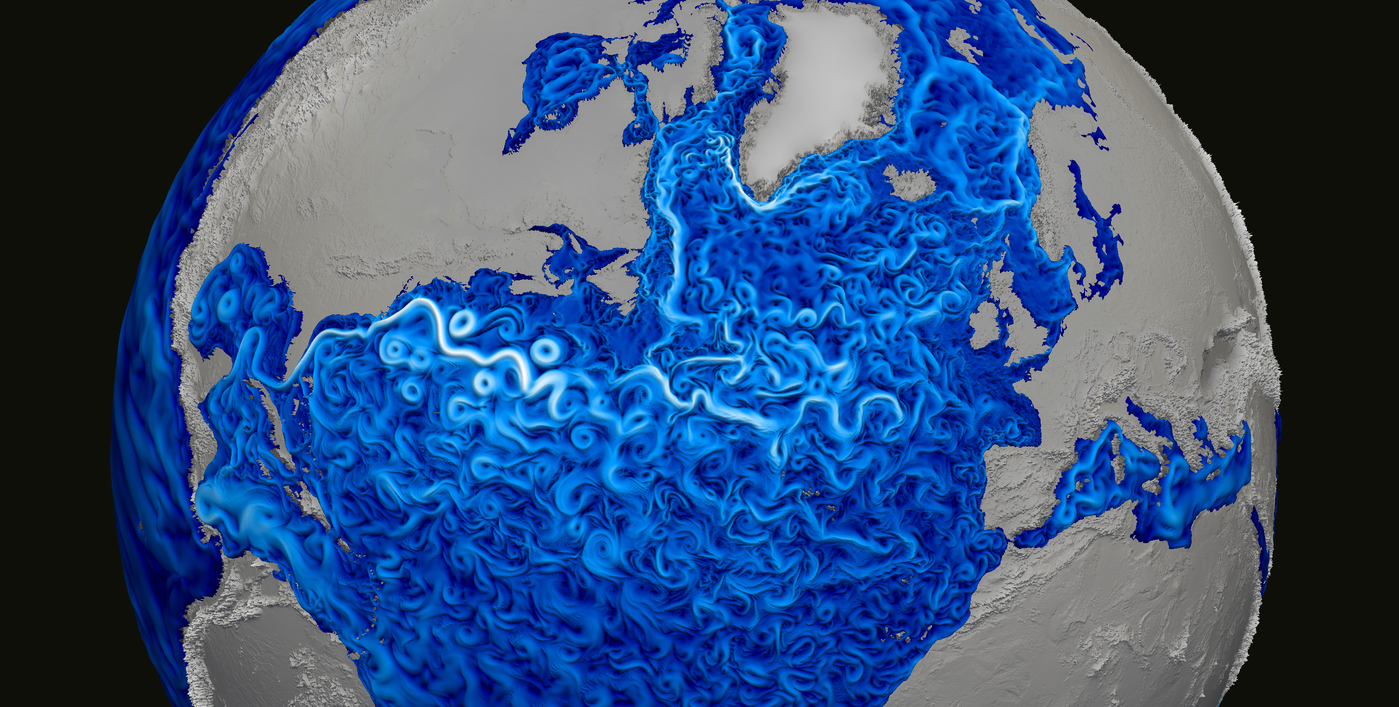
\includegraphics[width=\paperwidth,height=\paperheight,keepaspectratio]{ocean/figures/cover_V3_KE_NA37-7km_cropped_d.png}%
}}}

\newcommand{\core}{ocean}

\begin{document}
\AddToShipoutPicture*{\BackgroundPic}

\title{
\Huge MPAS-Ocean Model User's Guide \\
\LARGE Version: \version}

\author{
\LARGE Climate, Ocean, Sea-Ice Modeling Team\\ \\
\LARGE Los Alamos National Laboratory
}

\date{November 18, 2014}

\maketitle

\chapter*{Copyright}
\label{chap:copyright}
{\bf Copyright \copyright 2013,  Los Alamos National Security, LLC (LANS) (LA-CC-13-047)
and the University Corporation for Atmospheric Research (UCAR).} \\

All rights reserved.  \\

LANS is the operator of the Los Alamos National Laboratory under Contract No.
DE-AC52-06NA25396 with the U.S. Department of Energy.  UCAR manages the National
Center for Atmospheric Research under Cooperative Agreement ATM-0753581 with the
National Science Foundation.  The U.S. Government has rights to use, reproduce,
and distribute this software.  NO WARRANTY, EXPRESS OR IMPLIED IS OFFERED BY
LANS, UCAR OR THE GOVERNMENT AND NONE OF THEM ASSUME ANY LIABILITY FOR THE USE
OF THIS SOFTWARE.  If software is modified to produce derivative works, such
modified software should be clearly marked, so as not to confuse it with the
version available from LANS and UCAR. \\

Additionally, redistribution and use in source and binary forms, with or without
modification, are permitted provided that the following conditions are met: \\

1) Redistributions of source code must retain the above copyright notice, this
list of conditions and the following disclaimer. \\

2) Redistributions in binary form must reproduce the above copyright notice,
this list of conditions and the following disclaimer in the documentation and/or
other materials provided with the distribution. \\

3) None of the names of LANS, UCAR or the names of its contributors, if any, may
be used to endorse or promote products derived from this software without
specific prior written permission. \\

THIS SOFTWARE IS PROVIDED BY THE COPYRIGHT HOLDERS AND CONTRIBUTORS "AS IS" AND
ANY EXPRESS OR IMPLIED WARRANTIES, INCLUDING, BUT NOT LIMITED TO, THE IMPLIED
WARRANTIES OF MERCHANTABILITY AND FITNESS FOR A PARTICULAR PURPOSE ARE
DISCLAIMED. IN NO EVENT SHALL THE COPYRIGHT HOLDER OR CONTRIBUTORS BE LIABLE FOR
ANY DIRECT, INDIRECT, INCIDENTAL, SPECIAL, EXEMPLARY, OR CONSEQUENTIAL DAMAGES
(INCLUDING, BUT NOT LIMITED TO, PROCUREMENT OF SUBSTITUTE GOODS OR SERVICES;
LOSS OF USE, DATA, OR PROFITS; OR BUSINESS INTERRUPTION) HOWEVER CAUSED AND ON
ANY THEORY OF LIABILITY, WHETHER IN CONTRACT, STRICT LIABILITY, OR TORT
(INCLUDING NEGLIGENCE OR OTHERWISE) ARISING IN ANY WAY OUT OF THE USE OF THIS
SOFTWARE, EVEN IF ADVISED OF THE POSSIBILITY OF SUCH DAMAGE.
\newpage

\chapter*{Foreword}
\label{chap:foreword}

The MPAS-Albany Land Ice (MALI) is an unstructured-mesh land ice model (ice sheets or glaciers) capable of using enhanced 
horizontal resolution in selected regions of the land ice domain.  
MALI is built using the Model for Prediction Across Scales (MPAS) framework for developing variable resolution Earth System Model components 
and the Albany multi-physics code base for solution of coupled systems of partial-differential equations, which itself makes use of Trilinos solver libraries.  
MALI includes a three-dimensional, first-order momentum balance solver (``Blatter-Pattyn") by linking to the Albany-LI ice sheet velocity solver,
as well as an explicit shallow ice velocity solver.
Evolution of ice geometry and tracers is handled through an explicit first-order
horizontal advection scheme with vertical remapping.
Evolution of ice temperature is treated using operator splitting of vertical diffusion and horizontal advection and can be configured to use either a temperature or enthalpy formulation.  
MALI includes a mass-conserving subglacial hydrology model that supports distributed and/or channelized drainage and can optionally be coupled to ice dynamics.
Options for calving include ``eigencalving'', which assumes calving rate is proportional to extensional strain rates.
MALI has been evaluated against commonly used exact solutions and community benchmark experiments and shows the expected accuracy.
It has been used in land ice evolution experiments estimating potential for future sea-level rise from ice sheets 
(e.g., Ice2Sea international assessment project \citep{Shannon2013, edwards2014}).  
MALI is the glacier component of the Energy Exascale Earth System Model (E3SM) version 1.0
(\url{https://climatemodeling.science.energy.gov/projects/energy-exascale-earth-system-model}).

MPAS-Albany Land Ice is one component within the Model for Prediction Across Scales (MPAS) framework of climate model components
 that is developed in cooperation between Los Alamos National Laboratory (LANL) and the National Center for Atmospheric Research (NCAR).  
Functionality that is required by all cores, such as i/o, time management, block decomposition, etc, is developed collaboratively, and this code is shared across cores within the same repository.  
Each core then solves its own differential equations and physical parameterizations within this framework.  
This user's guide reflects the spirit of this collaborative process, where Part I, ``The MPAS Framework'', applies to all cores, 
and the remaining parts apply specifically to MPAS-Albany Land Ice.

MPAS-Albany Land Ice also makes use of the Albany/LI velocity solver (formally Albany/FELIX) for implementation of the first-order
velocity solver.  Not all details of running and configuring that velocity solver are covered in this User's Guide.  
We refer the user to Albany's website for more information about installing and running Albany: \url{https://github.com/gahansen/Albany}

MPAS-Albany Land Ice is described by a model description paper currently in review in Geoscientific Model Descriptions at:
\url{https://www.geosci-model-dev-discuss.net/gmd-2018-78/}
Much of the information in this User's Guide is derived from the text of that paper.


A history of releases of the Land Ice core within the MPAS version numbering scheme is as follows:

\begin{tabular}{p{1.5cm} p{3.7cm} p{10cm}} 
\hline\hline version & date & description  \\
\hline 
6.0 & April 17, 2018 & Addition of Albany FO velocity solver, thermal solver, subglacial hydrology model, calving, analysis members, coupling to E3SM.\\
\hline 
3.0 & November 18, 2014 & Fix bug in SIA slope calculation.  Introduction of run-time I/O streams. \\
\hline 
2.0 & November 15, 2013 & Initial public release of Land Ice core (SIA velocity solver only) \\
\hline 
\end{tabular} 

Information about MPAS-Albany Land Ice, including the most recent code, user's guide, and test cases, may be found at \url{http://mpas-dev.github.com}.  This user's guide refers to version \version.

\vspace{8pt}
\noindent
{\bf Contributors to this guide:}\\
Matt Hoffman, Stephen Price, Mauro Perego\\
{\bf Additional contributors to MPAS Framework sections:}\\
Michael Duda, Douglas Jacobsen

\vspace{8pt}
\noindent
{\it Funding for the development of MPAS-Albany Land Ice was provided by the United States Department of Energy, Office of Science.}





\chapter*{History}
\label{chap:history}

A history of MPAS-O releases follows: \\


\begin{tabular}{ll p{4in}} 
\hline\hline version & date & description of new additions  \\
\hline 
3.0 & November 18th, 2014 & 
GM mesoscale eddy parameterization, CVMix vertical mixing module (includes KPP), forward/analysis modes, and run-time configurable i/o streams \\
\hline 
2.0 & November 15th, 2013 & 
Surface forcing capabilities, Arbitrary Lagrangian-Eulerian vertical grid for z-level, z-star, z-tilde, sigma, idealized isopycnal \\
\hline 
1.0 & June 14th, 2013 & Primitive equation (hydrostatic) ocean model for idealized and realistic global domains using split-explicit time-stepping, flux-corrected transport advection, Jackett-McDougall EOS, harmonic/biharmonic horizontal mixing, and implicit Richardson number-based vertical mixing.  Vertical coordinate may be z-level or z-star with partial bottom cells, or idealized isopycnal. \\
\hline 
0.0 & June 14th, 2013 & Initial pre-release of MPAS \\
\hline 
\end{tabular} 



\newpage


\tableofcontents

\chapter{MPAS-Ocean Quick Start Guide}
\label{chap:quick_start}

This chapter provides MPAS-Ocean users with a quick start description of how to
build and run the model. It is meant merely as a brief overview of the process,
while the more detailed descriptions of each step are provided in later
sections.

In general, the build process follows the following steps.  See Chapter 
\ref{chap:tested-configurations} for recommended versions.

\begin{enumerate}
	\item Build MPI Layer (OpenMPI, MVAPICH2, etc.)
	\item Build serial NetCDF library
	\item Build Parallel-NetCDF library
	\item Build Parallel I/O library
	\item (Optional) Build METIS library and executables
	\item Checkout MPAS-Ocean from repository
	\item Build ocean core (e.g.\ {\tt make CORE=ocean})
\end{enumerate}

After step 7, an executable should be created called ocean\_model. Once the executable is built, one can begin the run process as follows:

\begin{enumerate}
	\item Download a run directory from \url{http://mpas-dev.github.com}, ``MPAS-Ocean Download''
	\item Copy or link executable to run directory.
	\item (Optional) Edit namelist.ocean to have the proper parameters. In particular, you may change the simulation length with {\tt config\_run\_duration = '0000\_06:00:00'}, which shows {\tt DAYS\_H:M:S}.
	\item (Optional) Create additional graph files using METIS executable (pmetis or gpmetis depending on version).  A graph file is required for each processor count you want to use.  See Section \ref{sec:metis}
	\item Run MPAS-Ocean (e.g.\ {\tt mpirun -np 8 ocean\_model}).
	\item If run was successful, last line of {\tt log.ocean.0000.out} shows {\tt Logging complete.}
	\item Visualize output file and perform analysis.  Output file is typically named {\tt output.nc}.  See Chapters \ref{chap:mpas_visualization} and \ref{chap:ocean_visualization}.
\end{enumerate}

\chapter{Support Policy}
\label{chap:ocean-support}
This chapter will define the current support policy for the MPAS-Ocean team.

Currently, support for MPAS-Ocean is only provided through two mediums. The
first being the issue tracker on the
\href{https://github.com/MPAS-Dev/MPAS-Release/issues?state=open}{MPAS-Release
github site}, and the second being the
\href{https://groups.google.com/forum/#!forum/mpas-users}{MPAS-Ocean user
mailing list}. 

For the time being, MPAS-Ocean developers will only support setups provided
through the release web-site. At present, we do not have enough resources to
provide support for model development exercises, and modified test cases. Users
interested in modifying MPAS-O source code are referred to the MPAS-Developer's
guide on the \href{http://mpas-dev.github.io/}{MPAS website}.

For questions about the variables and namelist options, users are referred to
Chapters  \ref{chap:namelist_sections} and \ref{chap:variable_sections} in this
users guide.

\section{Reporting bugs}
\label{sec:bug-reports}
Bugs can be confirmed through the mailing list, but a bug report should be
made through the issue tracker on the github website.
It is expected that the user provides the information requested
\href{https://gist.github.com/douglasjacobsen/5868321}{in this form} when
reporting a bug.

This enables the developers to more easily try to reproduce the issue and
figure out what the cause is.



\part{The MPAS Framework}
\chapter{Building MPAS}
\label{chap:mpas_build_instructions}

\section{Prequisites}

To build MPAS, compatible C and Fortran compilers are required. Additionally, the MPAS software relies on the PIO parallel I/O library to read and write model fields, and the PIO library requires the standard netCDF library as well as the parallel-netCDF library from Argonne National Labs. All libraries must be compiled with the same compilers that will be used to build MPAS. Section \ref{sec:build_io} summarizes the basic procedure of installing the required I/O libraries for MPAS.

In order for the MPAS makefiles to find the PIO, parallel-netCDF, and netCDF include files and libraries, the environment variables {\tt PIO}, {\tt PNETCDF}, and {\tt NETCDF} should be set to the root installation directories of the PIO, parallel-netCDF, and netCDF installations, respectively. Newer versions of the netCDF library use a separate Fortran interface library; the top-level MPAS Makefile attempts to add {\tt -lnetcdff} to the linker flags, but some linkers require that {\tt -lnetcdff} appear before {\tt -lnetcdf}, in which case {\tt -lnetcdff} will need to be manually added just before {\tt -lnetcdf} in the specification of {\tt LIBS} in the top-level Makefile.

An MPI installation such as MPICH or OpenMPI is also required, and there is no option to build a serial version of the MPAS executables. There is currently no support for shared-memory parallelism with OpenMP within the MPAS framework.


\section{Compiling I/O Libraries}
\label{sec:build_io}

{\bf NOTE:} It's important to note the MPAS Developers are not responsible for any of the libraries that are used within MPAS. Support for specific libraries should be taken up with the respective developer groups.

Although most recent versions of the I/O libraries should work, the most tested versions of these libraries are: netCDF 4.1.3, parallel-netCDF 1.3.1, and PIO 1.4.1. The netCDF and parallel-netCDF libraries must be installed before building PIO library.

All commands are presented for csh, and will not work if pasted into another shell. Please translate them to the appropraite commands in your shell.

\subsection{netCDF}

Version 4.1.3 of the netCDF library may be downloaded from \url{http://www.unidata.ucar.edu/downloads/netcdf/netcdf-4\_1\_3/index.jsp}.
Assuming the gfortran and gcc compilers will be used, the following shell commands are generally sufficient to install netCDF.

\vspace{12pt}
{\tt > setenv FC gfortran}

{\tt > setenv F77 gfortran} 

{\tt > setenv F90 gfortran}

{\tt > setenv CC gcc} 

{\tt > ./configure --prefix=XXXXX --disable-dap --disable-netcdf-4 --disable-cxx \hfill\break --disable-shared --enable-fortran} 

{\tt > make all check}

{\tt > make install}
\vspace{12pt}

Here, {\tt XXXXX} should be replaced with the directory that will serve as the root installation directory for netCDF.
{\em Before proceeding to compile PIO the {\tt NETCDF\_PATH} environment variable should be set to the netCDF root installation directory.}

Certain compilers require addition flags in the CPPFLAGS environment variable. Please refer to the netCDF installation instructions for these flags.

\subsection{parallel-netCDF}

Version 1.3.1 of the parallel-netCDF library may be downloaded from \url{https://trac.mcs.anl.gov/projects/parallel-netcdf/wiki/Download}.
Assuming the gfortran and gcc compilers will be used, the following shell commands are generally sufficient to install parallel-netCDF.

\vspace{12pt}
{\tt > setenv MPIF90 mpif90}

{\tt > setenv MPIF77 mpif90} 

{\tt > setenv MPICC mpicc}  

{\tt > ./configure --prefix=XXXXX} 

{\tt > make}

{\tt > make install}
\vspace{12pt}

Here, {\tt XXXXX} should be replaced with the directory that will serve as the root installation directory for parallel-netCDF.
{\em Before proceeding to compile PIO the {\tt PNETCDF\_PATH} environment variable should be set to the parallel-netCDF root installation directory.}


\subsection{PIO}

Instructions for building PIO can be found at \url{http://www.cesm.ucar.edu/models/pio/}. Please refer to these instructions for building PIO.

After PIO is built, and installed the PIO enviroment variable needs to be
defined to point at the directory PIO is installed into. Older versions of PIO
cannot be installed, and the PIO environment variable needs to be set to the
directory where PIO was built instead.

\section{Compiling MPAS}

{\bf \em Before compiling MPAS, the {\tt NETCDF}, {\tt PNETCDF}, and {\tt PIO} environment variables must be set to the library installation directories as
described in the previous section. A {\tt CORE} variable also needs to either be defined or passed in during the make process. If {\tt CORE} is not specified, 
the build process will fail.}

The MPAS code uses only the `make' utility for compilation. Rather than employing a separate configuration step
before building the code, all information about compilers, compiler flags, etc., is contained in the top-level {\tt Makefile}; each
supported combination of compilers (i.e., a configuration) is included in the {\tt Makefile} as a separate make target, and the user selects among
these configurations by running {\tt make} with the name of a build target specified on the command-line, e.g.,

\vspace{12pt}
{\tt > make gfortran}
\vspace{12pt}

\noindent to build the code using the GNU Fortran and C compilers. Some of the available targets are listed in the table below, and additional
targets can be added by simply editing the {\tt Makefile} in the top-level directory.

\vspace{12pt}
\begin{longtable}{| l | l | l | l |}
\hline
Target & Fortran compiler & C compiler & MPI wrappers \\ \hline \hline
{\tt xlf} & xlf90 & xlc & mpxlf90 / mpcc \\ \hline
{\tt pgi} & pgf90 & pgcc & mpif90 / mpicc \\ \hline
{\tt ifort} & ifort & gcc & mpif90 / mpicc \\ \hline
{\tt gfortran} & gfortran & gcc & mpif90 / mpicc \\ \hline
{\tt g95} & g95 & gcc & mpif90 / mpicc \\ \hline
\end{longtable}
\vspace{12pt}

In order to get a more complete and up-to-date list of available tagets, one can use the following command within the top-level of MPAS. {\bf NOTE: }This command is known to not work with Mac OSX.
{\small
\begin{verbatim}
> make -rpn | sed -n -e '/^$/ { n ; /^[^ ]*:/p }' | sed "s/: *.*$//g"
\end{verbatim}
}

The MPAS framework supports multiple {\em cores} --- currently a shallow water
model, an ocean model, a non-hydrostatic atmosphere model, and a non-hydrostatic atmosphere initialization core --- so the build
process must be told which core to build. This is done by either setting the environment variable
{\tt CORE} to the name of the model core to build, or by specifying the core to be built explicitly on the command-line
when running {\tt make}. For the shallow water core, for example, one may run either

\vspace{12pt}
{\tt > setenv CORE sw}

{\tt > make gfortran}
\vspace{12pt}

\noindent or

\vspace{12pt}
{\tt > make gfortran CORE=sw}
\vspace{12pt}

If the {\tt CORE} environment variable is set and a core is specified on the command-line, the command-line value takes precedence; if no core
is specified, either on the command line or via the {\tt CORE} environment variable, the build process will stop with an error message stating such.
Assuming compilation is successful, the model executable, named {\tt \$\{CORE\}\_model.exe} (e.g., {\tt sw\_model.exe}), should
be created in the {\tt src/} subdirectory, and a symbolic link to the model executable 
should exist in the top-level MPAS directory.

In order to get a list of available cores, one can simply run the top-level {\tt Makefile} without setting the {\tt CORE} environment variable, or passing the core via the command-line. And example of the output from this can be seen below.

{\small
\begin{verbatim}
> make
( make error )
make[1]: Entering directory `/home/douglasj/Documents/svn-mpas-model.cgd.ucar.edu/trunk/mpas'

Usage: make target CORE=[core] [options]

Example targets:
ifort
gfortran
xlf
pgi

Availabe Cores:
atmosphere
init_atmosphere
ocean
sw

Available Options:
DEBUG=true    - builds debug version. Default is optimized version.
USE_PAPI=true - builds version using PAPI for timers. Default is off.
TAU=true      - builds version using TAU hooks for profiling. Default is off.

Ensure that NETCDF, PNETCDF, PIO, and PAPI (if USE_PAPI=true) are environment variables
that point to the absolute paths for the libraries.

************ ERROR ************
No CORE specified. Quitting.
************ ERROR ************

make[1]: Leaving directory `/home/douglasj/Documents/svn-mpas-model.cgd.ucar.edu/trunk/mpas'
\end{verbatim}
}

\section{Cleaning}

To remove all files  that were created when the model was built, including the model executable itself, {\tt make} may
be run for the `clean' target:

\vspace{12pt}
{\tt > make clean}
\vspace{12pt}

As with compiling, the core to be cleaned is specified by the {\tt CORE} environment variable, or by specifying a core explicitly on the command-line with {\tt CORE=}.


\section{Graph partitioning with METIS} 
\label{sec:metis}

% this section is also in mpas_grid_generation.tex.  When grid generation is included in a future release, delete this section from this chapter.

Before MPAS can be run in parallel, a mesh decomposition file with an appropriate number of 
partitions (equal to the number of MPI tasks that will be used) is required in the run directory.  A limited number of mesh decomposition files ({\tt graph.info.part.*}) are provided with each test case.  In order to create new mesh decomposition files for your desired number of partitions, begin with the provided {\tt graph.info} file and partition with METIS software (\url{http://glaros.dtc.umn.edu/gkhome/views/metis}). The serial graph partitioning program, METIS (rather than ParMETIS or hMETIS) should be sufficient for quickly partitioning any SCVT produced by the grid\_gen mesh generator.

After installing METIS, a {\tt graph.info} file may be partitioned into $N$ partitions by running

\vspace{12pt}
{\tt > gpmetis graph.info} $N$
\vspace{12pt}

\noindent The resulting file, {\tt graph.info.part.}$N$, can then be copied into the MPAS run directory
before running the model with $N$ MPI tasks.

\chapter{Grid Description}
\label{chap:mpas_grid_description}

This chapter provides a brief introduction to the common types of grids used in the MPAS framework. 

The MPAS grid system requires the definition of seven elements. These seven elements are composed of two types of {\it cells}, two types of {\it lines}, and three types of {\it points}. These elements are depicted in Figure \ref{figure:variablePosition} and defined in Table \ref{table:variablePosition}.  These elements can be defined on either the plane or the surface of the sphere. The two types of cells form two meshes, a primal mesh composed of Voronoi regions and a dual mesh composed of Delaunay triangles. Each corner of a primal mesh cell is uniquely associated with the ``center'' of a dual mesh cell and vice versa. So we define the two mesh as either a primal mesh (composed of cells $P_i$) or a dual mesh (composed of cells $D_v$). The center of any primal mesh cell, $P_i$, is denoted by ${\bf x}_i$ and the center of any the dual mesh cell, $D_v$, is denoted by ${\bf x}_v$. The boundary of a given primal mesh cell $P_i$ is composed of the set of lines that connect the ${\bf x}_v$ locations of associated dual mesh cells $D_v$. Similarly, the boundary of a given dual mesh cell $D_v$ is composed of the set of lines that connect the ${\bf x}_i$ locations of the associated primal mesh cells $P_i$. 

As shown in Figure \ref{figure:variablePosition}, a line segment that connects two primal mesh cell centers is uniquely associated with a line segment that connects two dual mesh cell centers. We assume that these two line segments cross and the point of intersection is labeled as ${\bf x}_e$. In addition, we assume that these two line segments are orthogonal as indicated in Figure \ref{figure:variablePosition}. Each ${\bf x}_e$ is associated with two distances: $d_e$ measures the distance between the primal mesh cells sharing ${\bf x}_e$ and $l_e$ measures the distance between the dual mesh cells sharing ${\bf x}_e$.

Since the two line segments crossing at ${\bf x}_e$ are orthogonal, these line segments form a convenient local coordinate system for each edge. At each ${\bf x}_e$ location a unit vector ${\bf n}_e$ is defined to be parallel to the line connecting primal mesh cells. A second unit vector ${\bf t}_e$ is defined such that ${\bf t}_e = {\bf k} \times {\bf n}_e$.

In addition to these seven element types, we require the definition of {\it sets of elements}. In all, eight different types of sets are required and these are defined and explained in Table \ref{table:gridConnectivity} and Figure \ref{figure:gridConnectivity}. The notation is always of the form of, for example, $i \in CE(e)$, where the LHS indicates the type of element to be gathered (cells) based on the RHS relation to another type of element (edges).

Table \ref{table:gridFileName} provides the names of all {\it elements} and all {\it sets of elements} as used in the MPAS framework.  Elements appear twice in the table when described in the grid file in more than one way, e.g. points are described with both cartesian and latitude/longitude coordinates. An ``ncdump -h'' of any MPAS grid, output or restart file will contain all variable names shown in second column of Table  \ref{table:gridFileName}.


\begin{table}[t]
\caption{Definition of elements used to build the MPAS grid.}
\label{table:variablePosition}
\begin{center}
\begin{tabular}{lll}
\hline\hline
$Element$ & $Type$ & $Definition$\\
\hline
 ${\bf x}_i$   & point             & location of center of primal-mesh cells \\
 ${\bf x}_v$  &  point            & location of center of dual-mesh cells \\
 ${\bf x}_e$  & point             & location of edge points where velocity is defined \\
 $d_{e}$       & line segment & distance between neighboring ${\bf x}_i$ locations \\
 $l_{e}$       & line segment & distance between neighboring ${\bf x}_v$ locations \\
 $P_i$         & cell                 & a cell on the primal-mesh \\
 $D_v$        & cell                 & a cell on the dual-mesh \\
\hline
\end{tabular}
\end{center}
\end{table}
%
\begin{table}[t]
\caption{Definition of element groups used to reference connections in the MPAS grid. Examples are provided in Figure \ref{figure:gridConnectivity}.}
\label{table:gridConnectivity}
\begin{center}
\begin{tabular}{lll}
\hline\hline
$Syntax$ & $ouptut$\\
\hline
 $e \in EC(i) $   & set of edges that define the boundary of $P_i$. \\
 $e \in EV(v) $     & set of edges that define the boundary of $D_v$. \\
 $i \in CE(e) $                 & two primal-mesh cells that share edge $e$. \\
 $i \in CV(v) $  &  set of primal-mesh cells that form the vertices of dual mesh cell $D_v$. \\
 $v\in VE(e) $  & the two dual-mesh cells that share edge $e$. \\
 $v \in VI(i) $   & the set of dual-mesh cells that form the vertices of primal-mesh cell $P_i$. \\
 $e \in ECP(e)$ & edges of cell pair meeting at edge $e$. \\
 $e \in EVC(v,i)$ & edge pair associated with vertex $v$ and mesh cell $i$. \\
\hline
\end{tabular}
\end{center}
\end{table}
%

\begin{table}[t]
\caption{Variable names used to describe a MPAS grid.}
\label{table:gridFileName}
\begin{center}
\begin{tabular}{llll}
\hline\hline
$Element$ & $Name$ & $Size$ & $Comment$\\
\hline
 ${\bf x}_i$   & \{x,y,z\}Cell          & nCells  & cartesian location of ${\bf x}_i$  \\
 ${\bf x}_i$   & \{lon,lat\}Cell        & nCells  & longitude and latitude of  ${\bf x}_i$  \\
 ${\bf x}_v$   & \{x,y,z\}Vertex      & nVertices  & cartesian location of ${\bf x}_v$  \\
 ${\bf x}_v$   & \{lon,lat\}Vertex    & nVertices  & longitude and latitude of  ${\bf x}_v$  \\
 ${\bf x}_e$   & \{x,y,z\}Edge          & nEdges  & cartesian location of ${\bf x}_e$  \\
 ${\bf x}_e$   & \{lon,lat\}Edge        & nEdges  & longitude and latitude of  ${\bf x}_e$  \\
 $d_{e}$       & dcEdge                   & nEdges  & distance between ${\bf x}_i$ locations\\
 $l_{e}$         & dvEdge             & nEdges &  distance between ${\bf x}_v$ locations \\
  &  & & \\
 $e \in EC(i) $   &  edgesOnCell  & (nEdgesMax,nCells) & edges that define $P_i$. \\
 $e \in EV(v) $     & edgesOnVertex &  (3,nCells) & edges that define $D_v$. \\
 $i \in CE(e) $      & cellsOnEdge &  (2,nEdges) &  primal-mesh cells that share edge $e$. \\
 $i \in CV(v) $  &   cellsOnVertex &  (3,nVertices) &  primal-mesh cells that define $D_v$. \\
 $v\in VE(e) $  & verticesOnEdge &  (2,nEdges) &    dual-mesh cells that share edge $e$. \\
 $v \in VI(i) $   & verticesOnCell &  (nEdgesMax,nCells) & vertices that define $P_i$. \\
\hline
\end{tabular}
\end{center}
\end{table}
%


%
\begin{figure}[t]
  \noindent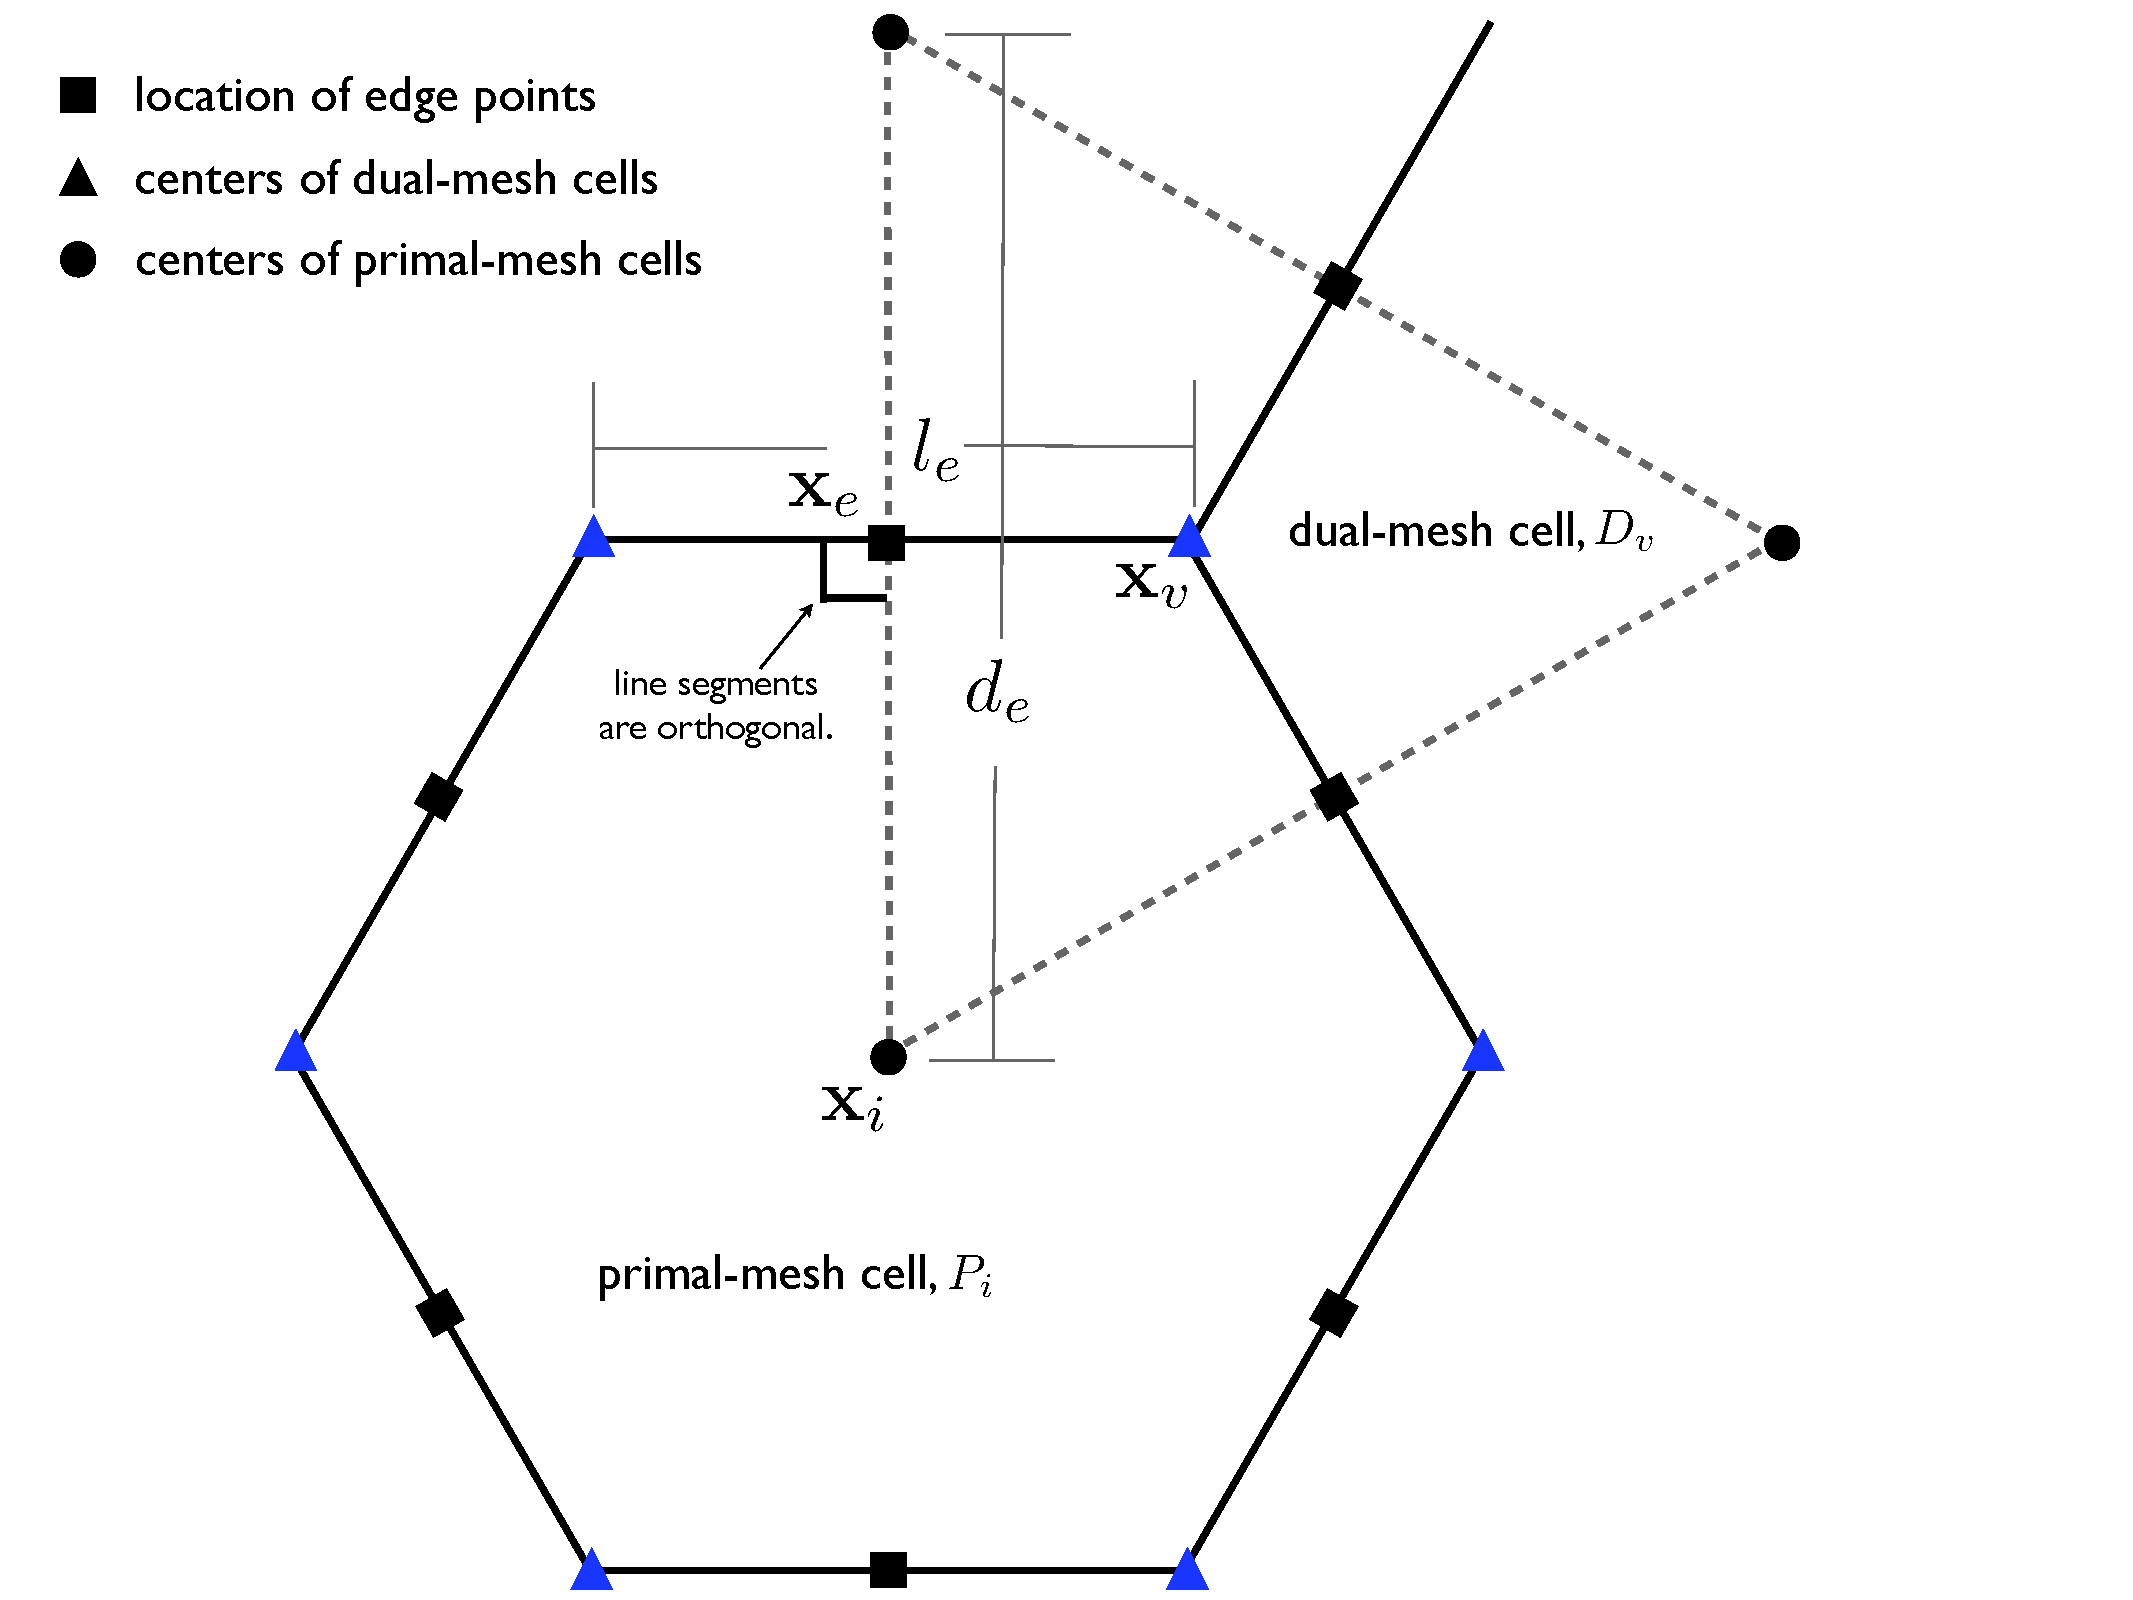
\includegraphics[width=16cm,angle=0]{./shared/figures/variablePosition.pdf}\\
  \caption{Definition of elements used to build the MPAS grid. Also see Table \ref{table:variablePosition}.}
  \label{figure:variablePosition}
\end{figure}

%
\begin{figure}[t]
   \noindent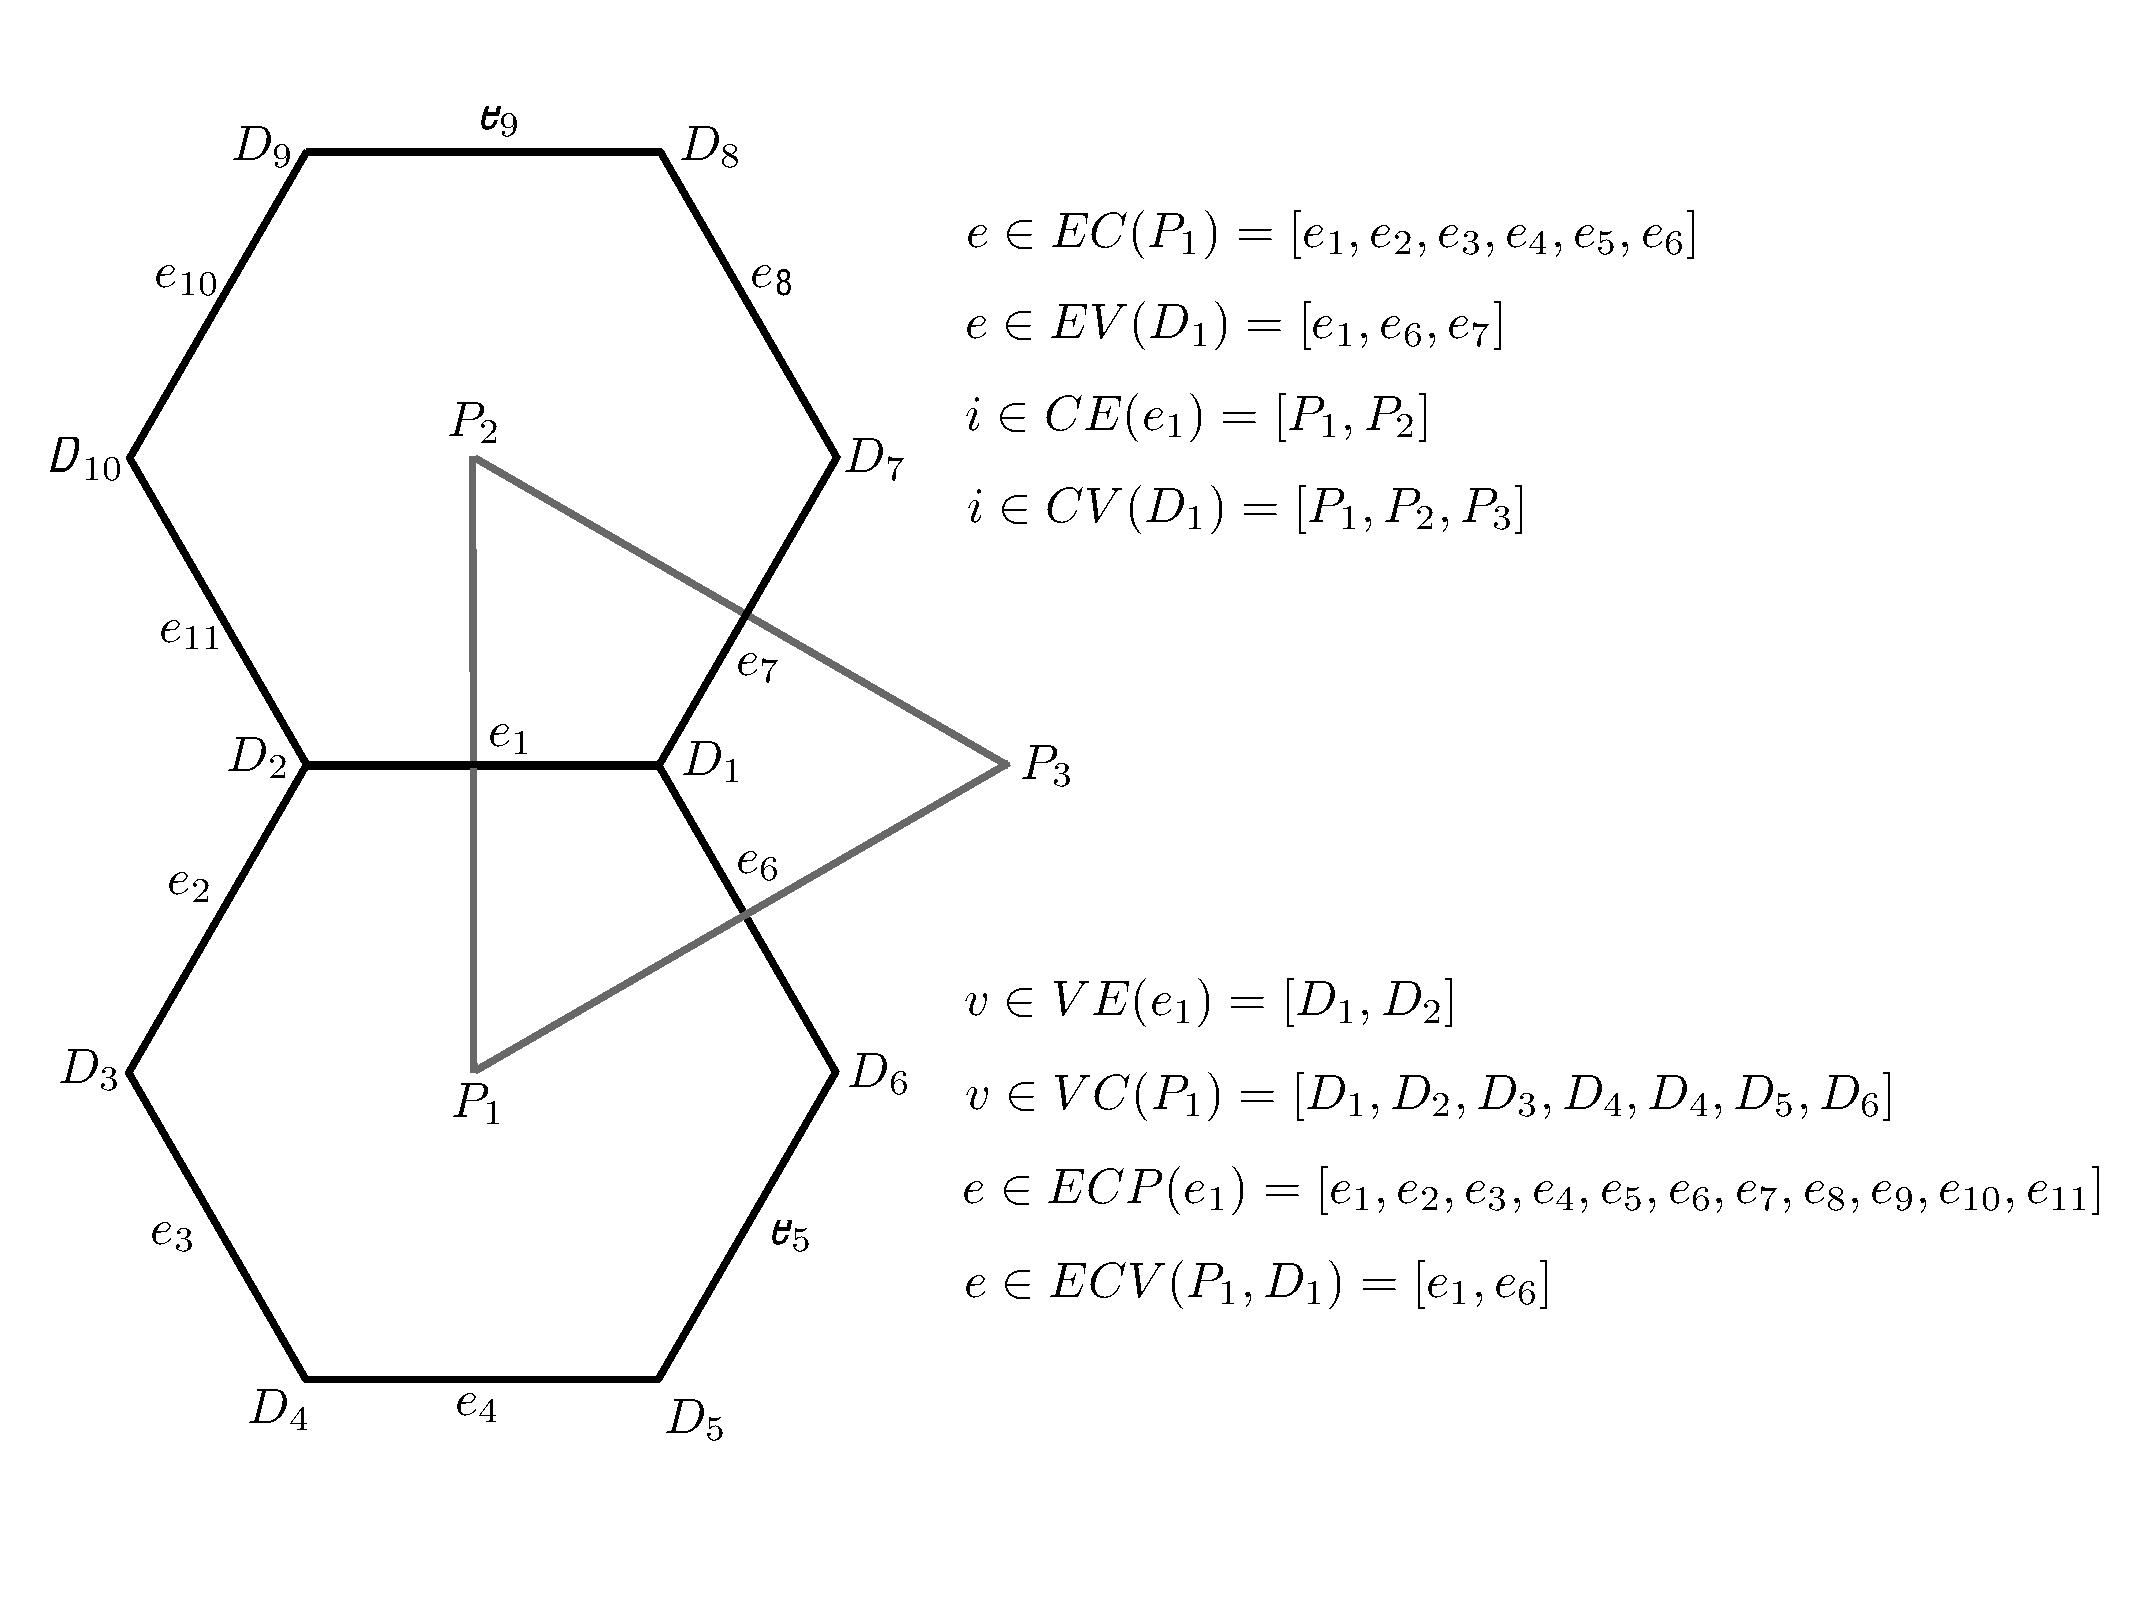
\includegraphics[width=16cm,angle=0]{./shared/figures/gridConnectivity.pdf}\\
  \caption{Definition of element groups used to reference connections in the MPAS grid. Also see Table \ref{table:gridConnectivity}.}
  \label{figure:gridConnectivity}
\end{figure}



\chapter{Configuring Model Input and Output}
\label{chap:mpas_io}

\newlength{\immindent}
\settowidth{\immindent}{{\tt <immutable\_stream }}


\newlength{\mutindent}
\settowidth{\mutindent}{{\tt <stream }}

The reading and writing of model fields in MPAS is handled by user-configurable {\em streams}. 
A stream represents a fixed set of model fields, together with dimensions and attributes, that are
all written or read together to or from the same file or set of files. Each MPAS model core may define
its own set of default streams that it typically uses for reading initial conditions, for writing and reading
restart fields, and for writing additional model history fields. Besides these default streams, users may define
new streams to, e.g., write certain diagnostic fields at a higher temporal frequency than the usual model
history fields.

Streams are defined in XML configuration files that are created at build time for each model core. The name
of this XML file is simply `streams.' suffixed with the name of the core. For example, the streams for
the {\em sw} (shallow-water) core are defined in a file named `streams.sw'. An XML stream
file may further reference other text files that contain lists of the model fields that are read or written in
each of the streams defined in the XML stream file.

Changes to the XML stream configuration file will take effect the next time an MPAS core is run; there is no need
to re-compile after making modifications to the XML files. As described in the next section, it is therefore possible, e.g.,
to change the interval at which a stream is written, the template for the filenames associated with a stream, or the 
set of fields that are written to a stream, without the need to re-compile any code.

Two classes of streams exist in MPAS: {\em immutable} streams and {\em mutable} streams. Immutable streams
are those for which the set of fields that belong to the stream may not be modified at model run-time; however, it is
possible to modify the interval at which the stream is read or written, the filename template describing the files
containing the stream on disk, and several other parameters of the stream. In contrast, all aspects of mutable streams,
including the set of fields that belong to the stream, may be modified at run-time. The motivation for the creation of
two stream classes is the idea that an MPAS core may not function correctly if certain fields are not read in upon 
model start-up or written to restart files, and it is therefore not reasonable for users to modify this set of required fields 
at run-time. An MPAS core developer may choose to implement such streams as immutable streams. Since fields may
not be added to an immutable stream at run-time, new immutable streams may not be defined at run-time, and the only 
type of new stream that may be defined at run-time is the mutable stream type.

\section{XML stream configuration files}
\label{sec:xml_stream_format} 

The XML stream configuration file for an MPAS core always has a parent XML {\em element} named {\tt streams}, within which 
individual streams are defined:

\vspace{12pt}
\noindent {\tt <streams>} \newline
\newline
\hspace*{1cm}... one or more stream definitions ... \newline
\newline
\noindent {\tt </streams>} \newline
\vspace{12pt}

Immutable streams are defined with the {\tt immutable\_stream} element, and mutable streams are defined with the {\tt stream}
element: 

\vspace{12pt}
\noindent {\tt <immutable\_stream name="initial\_conditions"} \newline
\hspace*{\immindent}{\tt type="input"} \newline
\hspace*{\immindent}{\tt filename\_template="init.nc"} \newline
\hspace*{\immindent}{\tt input\_interval="initial\_only"} \newline
\hspace*{\immindent}{\tt />} \newline
\vspace{12pt} \newline
\noindent {\tt <stream name="history"} \newline
\hspace*{\mutindent}{\tt type="output"} \newline
\hspace*{\mutindent}{\tt filename\_template="output.\$Y-\$M-\$D\_\$h.\$m.\$s.nc"} \newline
\hspace*{\mutindent}{\tt output\_interval="6:00:00" >} \newline
\newline
\hspace*{1cm}... model fields belonging to this stream ... \newline
\newline
\noindent {\tt </stream>} \newline
\vspace{12pt}

As shown in the example stream definitions, above, both classes of stream have the following required attributes:

\begin{itemize}
\item {\tt name} --- A unique name used to refer to the stream.
\item {\tt type} --- The type of stream, either {\tt "input"}, {\tt "output"}, {\tt "input;output"}, or {\tt "none"}. A stream may be both an input
and an output stream (i.e., {\tt "input;output"}) if, for example, it is read once at model start-up to provide initial conditions and thereafter written 
periodically to provide model checkpoints. A stream may be defined as neither input nor output (i.e., {\tt "none"}) for the purposes of defining a 
set of fields for inclusion other streams. Note that, for immutable streams, the type attribute may not be changed at run-time.
\item {\tt filename\_template} --- The template for files that exist or will be created by the stream. The filename template may include any of the
following variables, which are expanded based on the simulated time at which files are first created.
\begin{itemize}
\item {\tt \$Y} --- Year
\item {\tt \$M} --- Month
\item {\tt \$D} --- Day of the month
\item {\tt \$d} --- Day of the year
\item {\tt \$h} --- Hour
\item {\tt \$m} --- Minute
\item {\tt \$s} --- Second
\end{itemize}
A filename template may include either a relative or an absolute path, in which case MPAS will attempt to create any directories 
in the path that do not exist, subject to filesystem permissions.
\item {\tt input\_interval} --- For streams that have type {\tt "input"} or {\tt "input;output"}, the interval, beginning at the model initial time,
at which the stream will be read. Possible values include a time interval specification in the format {\tt "YYYY-MM-DD\_hh:mm:ss"}; the value 
{\tt "initial\_only"}, which specifies that the stream is read only once at the model initial time; or the value {\tt "none"}, which specifies that 
the stream is not read during a model run.
\item {\tt output\_interval} --- For streams that have type {\tt "output"} or {\tt "input;output"}, the interval, beginning at the model initial time,
at which the stream will be written. Possible values include a time interval specification in the format {\tt "YYYY-MM-DD\_hh:mm:ss"}; the value 
{\tt "initial\_only"}, which specifies that the stream is written only once at the model initial time; or the value {\tt "none"}, which specifies that 
the stream is not written during a model run.
\end{itemize}

Finally, the set of fields that belong to a mutable stream may be specified with any combination of the following elements. Note that, for 
immutable streams, no fields are specified at run-time in the XML configuration file.

\begin{itemize}
\item {\tt var} --- Associates the specified variable with the stream. The variable may be any of those defined in an MPAS core's Registry.xml file, but may
not include individual constituent arrays from a var\_array.
\item {\tt var\_array} --- Associates all constituent variables in a var\_array, defined in an MPAS core's Registry.xml file, with the stream.
\item {\tt var\_struct} --- Associates all variables in a var\_struct, defined in an MPAS core's Registry.xml file, with the stream.
\item {\tt stream} --- Associates all explicitly associated fields in the specified stream with the stream; streams are not recursively included.
\item {\tt file} --- Associates all variables listed in the specified text file, with one field per line, with the stream.
\end{itemize}

\section{Optional stream attributes}
\label{sec:optional_stream_atts} 

Besides the required attributes described in the preceding section, several additional, optional attributes may be added to
the definition of a stream.

\begin{itemize}
\item {\tt filename\_interval} --- The interval between the timestamps used in the construction of the names of files associated with
a stream. Possible values include a time interval specification in the format {\tt "YYYY-MM-DD\_hh:mm:ss"}; the value {\tt "none"}, indicating
that only one file containing all times is associated with the stream; the value {\tt "input\_interval"} that, for input type streams, indicates that
each time to be read from the stream will come from a unique file; or the value {\tt "output\_interval"} that, for output type streams, indicates 
that each time to be written to the stream will go to a unique file whose name is based on the timestamp of the data being written. The default
value is {\tt "input\_interval"} for input type streams and {\tt "output\_interval"} for output type streams. For streams of type {\tt "input;output"}, the
default filename interval is {\tt "input\_interval"} if the input interval is an interval (i.e., not {\tt "initial\_only"}), or {\tt "output\_interval"} otherwise. 
Refer to Section \ref{sec:filename_interval_example}
for an example of the use of the filename\_interval attribute.
\item {\tt reference\_time} --- A time that is an integral number of filename intervals from the timestamp of any file associated with the stream.
The default value is the start time of the model simulation. Refer to Section \ref{sec:reference_time_example} for an example of 
the use of the reference\_time attribute.
\item {\tt clobber\_mode} --- Specifies how a stream should handle attempts to write to a file that already exists. Possible values
for the mode include:
\begin{itemize}
\item {\tt "overwrite"} --- The stream is allowed to overwrite records in existing files and to append new records 
to existing files; records not explicitly written to are left untouched.
\item {\tt "truncate"} or {\tt "replace\_files"} --- The stream is allowed to overwrite existing files, which are first truncated 
to remove any existing records; this is equivalent to replacing any existing files with newly created files of the same name.
\item {\tt "append"} --- The stream is only allowed to append new records to existing files; existing records may not be overwritten.
\item {\tt "never\_modify"} --- The stream is not allowed to modify existing files in any way.
\end{itemize}
The default clobber mode for streams is {\tt "never\_modify"}. Refer to Section \ref{sec:append_example} for an example of the use of
the clobber\_mode attribute.
\item {\tt precision} --- The precision with which real-valued fields will be written or read in a stream. Possible values include 
{\tt "single"} for 4-byte real values, {\tt "double"} for 8-byte real values, or {\tt "native"}, which specifies that real-valued fields
will be written or read in whatever precision the MPAS core was compiled. The default value is {\tt "native"}. Refer to Section \ref{sec:filename_interval_example}
for an example of the use of the precision attribute.
\item {\tt packages} --- A list of packages attached to the stream. A stream will be active (i.e., read or written) only if at least one of 
the packages attached to it is active, or if no packages at all are attached. Package names are provided as a semi-colon-separated
list. Note that packages may only be defined in an MPAS core's Registry.xml file at build time. By default, no packages are attached
to a stream.
\item {\tt io\_type} --- The underlying library and file format that will be used to read or write a stream. Possible values include:
\begin{itemize}
\item{\tt "pnetcdf"} --- Read/write the stream with classic large-file NetCDF files (CDF-2) using the ANL Parallel-NetCDF library.
\item{\tt "pnetcdf,cdf5"} --- Read/write the stream with large-variable files (CDF-5) using the ANL Parallel-NetCDF library. 
\item{\tt "netcdf"} --- Read/write the stream with classic large-file NetCDF files (CDF-2) using the Unidata serial NetCDF library.
\item{\tt "netcdf4"} --- Read/write the stream with HDF-5 files using the Unidata parallel NetCDF-4 library.
\end{itemize}
Note that the PIO library must have been built with support for the selected {\tt io\_type}. By default, all input and output streams are
read and written using the {\tt "pnetcdf"} option.
\end{itemize}

\section{Stream definition examples}
\label{sec:stream_example} 

This section provides several example streams that make use of the optional stream attributes described in Section \ref{sec:optional_stream_atts}.
All examples are of output streams, since it is more likely that a user will need to write additional fields than to read additional fields, which a model would need to be aware of; however, the concepts that are illustrated here translate directly to input streams as well.

\subsection{Example: a single-precision output stream with one month of data per file}
\label{sec:filename_interval_example}

In this example, the optional attribute specification {\tt filename\_interval="01-00\_00:00:00"} is added to force a new
output file to be created for the stream every month. Note that the general format for time interval specifications is {\tt YYYY-MM-DD\_hh:mm:ss},
where any leading terms can be omitted; in this case, the year part of the interval is omitted. To reduce the file size, the specification
{\tt precision="single"} is also added to force real-valued fields to be written as 4-byte floating-point values, rather than the default of 8 bytes.

\vspace{12pt}
\noindent {\tt <stream name="diagnostics"} \newline
\hspace*{\mutindent}{\tt type="output"} \newline
\hspace*{\mutindent}{\tt filename\_template="diagnostics.\$Y-\$M.nc"} \newline
\hspace*{\mutindent}{\tt filename\_interval="01-00\_00:00:00"} \newline
\hspace*{\mutindent}{\tt precision="single"} \newline
\hspace*{\mutindent}{\tt output\_interval="6:00:00" >} \newline
\newline
\hspace*{1cm}{\tt <var name="u10"/>} \newline
\hspace*{1cm}{\tt <var name="v10"/>} \newline
\hspace*{1cm}{\tt <var name="t2"/>} \newline
\hspace*{1cm}{\tt <var name="q2"/>} \newline
\newline
\noindent {\tt </stream>} \newline
\vspace{12pt}

The only fields that will be written to this stream are the hypothetical 10-m diagnosed wind components, the 2-m temperature, 
and the 2-m specific humidity variables. Also, note that the filename template only includes the year and month from the model 
valid time; this can be problematic when the simulation starts in the middle of a month, and a solution for this problem 
is illustrated in the example of Section \ref{sec:reference_time_example}.

\subsection{Example: appending records to existing output files}
\label{sec:append_example}

By default, streams will never modify existing files whose filenames match the name of a file that would otherwise be written
during the course of a simulation. However, when restarting a simulation that is expected to add more records to existing output 
files, it can be useful to instruct the MPAS I/O system to append these records, thereby modifying existing files. This may be 
accomplished with the {\tt clobber\_mode} attribute.

\vspace{12pt}
\noindent {\tt <stream name="diagnostics"} \newline
\hspace*{\mutindent}{\tt type="output"} \newline
\hspace*{\mutindent}{\tt filename\_template="diagnostics.\$Y-\$M.nc"} \newline
\hspace*{\mutindent}{\tt filename\_interval="01-00\_00:00:00"} \newline
\hspace*{\mutindent}{\tt precision="single"} \newline
\hspace*{\mutindent}{\tt clobber\_mode="append"} \newline
\hspace*{\mutindent}{\tt output\_interval="6:00:00" >} \newline
\newline
\hspace*{1cm}{\tt <var name="u10"/>} \newline
\hspace*{1cm}{\tt <var name="v10"/>} \newline
\hspace*{1cm}{\tt <var name="t2"/>} \newline
\hspace*{1cm}{\tt <var name="q2"/>} \newline
\newline
\noindent {\tt </stream>} \newline
\vspace{12pt}

In general, if MPAS were to attempt to write a record at a time that already existed in an output file, a clobber\_mode 
of `append' would not permit the write to take place, since this would modify existing data; in `append' mode, only new
records may be added. However, due to a peculiarity in the implementation of the `append' clobber mode, it may be 
possible for an output file to contain duplicate times. This can happen when the first record that is appended to 
an existing file has a timestamp not matching any in the file, after which, any record that is written --- regardless of 
whether its timestamp matches one already in the file --- will be appended to the end of the file. This situation may arise, 
for example, when restarting a model simulation with a shorter {\tt output\_interval} than was used in the original model simulation 
with an MPAS core that does not write the first output time for restart runs.

\subsection{Example: referencing filename intervals to a time other than the start time}
\label{sec:reference_time_example}

The example stream of the previous sections creates a new file each month during the simulation, and the filenames
contain only the year and month of the timestamp when the file was created. If a simulation begins at 00 UTC on the
first day of a month, then each file in the diagnostic stream will contain only output times that fall within the month
in the filename. However, if a simulation were to begin in the middle of a month --- for example, the month of June, 2014 --- 
the first diagnostics output file would have a filename of `diagnostics.2014-06.nc', but rather than containing only output
fields valid in June, it would contain all fields written between the middle of June and the middle of July, at which point
one month of simulation would have elapsed, and a new output file, `diagnostics.2014-07.nc', would be created.

In order to ensure that the file `diagnostics.2014-06.nc' contained only data from June 2014, the {\tt reference\_time}
attribute may be added such that the day, hour, minute, and second in the date and time represent the first day of the month
at 00 UTC. In this example, the year and month of the reference time are not important, since the purpose of the reference time
here is to describe to MPAS that the monthly filename interval begins (i.e., is referenced to) the first day of the month.

\vspace{12pt}
\noindent {\tt <stream name="diagnostics"} \newline
\hspace*{\mutindent}{\tt type="output"} \newline
\hspace*{\mutindent}{\tt filename\_template="diagnostics.\$Y-\$M.nc"} \newline
\hspace*{\mutindent}{\tt filename\_interval="01-00\_00:00:00"} \newline
\hspace*{\mutindent}{\tt reference\_time="2014-01-01\_00:00:00"} \newline
\hspace*{\mutindent}{\tt precision="single"} \newline
\hspace*{\mutindent}{\tt clobber\_mode="append"} \newline
\hspace*{\mutindent}{\tt output\_interval="6:00:00" >} \newline
\newline
\hspace*{1cm}{\tt <var name="u10"/>} \newline
\hspace*{1cm}{\tt <var name="v10"/>} \newline
\hspace*{1cm}{\tt <var name="t2"/>} \newline
\hspace*{1cm}{\tt <var name="q2"/>} \newline
\newline
\noindent {\tt </stream>} \newline
\vspace{12pt}

In general, the components of a timestamp, {\tt YYYY-MM-DD\_hh:mm:ss}, that are less significant than (i.e., to the right of) 
those contained in a filename template are important in a reference\_time. For example, with a {\tt filename\_template} that contained
only the year, the month component of the {\tt reference\_time} would become important to identify the month of the year on which
the yearly basis for filenames would begin.



% Grid generation is not included in MPAS release 1.0:
%\appendix{Generating meshes}
\label{chap:mpas_grid_generation}

This chapter describes the steps used to create the  spherical centroidal Voronoi tessellation (SCVT) meshes and mesh-decomposition files used by MPAS models.
Since it can take considerable time (often several days or more) to generate a mesh as described in \S \ref{sec:global_scvt}, it is recommended to obtain 
and use existing SCVT meshes from \url{http://www.mmm.ucar.edu/people/duda/mpas/} whenever possible; these meshes can be quickly
modified to shift or rotate the refinement regions over the geographic areas of interest using the utility program described in \S \ref{sec:grid_rotate}.

\section{Density functions}

In all MPAS models, the horizontal meshes are SCVTs with a C-grid staggering of
velocities. As their name suggests, SCVTs are Voronoi tessellations defined on the surface of a sphere, and in which the generating 
point for each Voronoi region is also the mass centroid of that region with respect to some {\em density function}. An overview of
the application of SCVTs to multi-resolution climate modeling is given in Ringler et al. (2008)
\footnote{Ringler, T., L. Ju and M. Gunzburger, 2008, A multiresolution method for climate system modeling: application of spherical centroidal Voronoi tessellations, {\em Ocean Dynamics}, 58 (5-6), 475-498. doi:10.1007/s10236-008-0157-2.}.

For the purposes of generating SCVTs, the central concern lies with the density function, $\rho$, which is a user-defined
function relating the relative resolutions in different regions of the mesh. Specifically, for two generating points of the 
SCVT, ${\bf x}_i$ and ${\bf x}_j$,
\[
{h_i \over h_j} \approx \left({\rho({\bf x}_j) \over \rho({\bf x}_i)} \right)^{1 \over 4},
\]
where $h_i$ and $h_j$ are the diameters of the Voronoi cells associated with ${\bf x}_i$ and ${\bf x}_j$, respectively.

In the mesh generation program global\_scvt, described in the next section, the density function is defined programatically in the Fortran function
{\tt density\_for\_point()}, which returns the value of the density function, $\rho({\bf x})$, given a location on the sphere, ${\bf x}$.
   
\section{The global\_scvt program}
\label{sec:global_scvt}

\subsection{Compilation}
                                                                                             
As a first step toward building the global\_scvt code, the environment variable                     
{\tt NETCDF} must be set to the root of the netCDF installation. Unlike with the MPAS model, separate make targets are not
defined for each compiler set, and it will generally be necessary to edit the top-level Makefile to set the compiler and compiler flags                 
that will be used to build global\_scvt; however, there are commented-out sections in the Makefile for using either of the ifort, pgf90, or gfortran compilers that may be uncommented or used as a starting point for other compilers. Also, if the netCDF installation has a separate Fortran interface library, {\tt -lnetcdff} will need to be added before {\tt -lnetcdf} in the Makefile. The global\_scvt program is parallelized with OpenMP, so if compiler support is available, OpenMP compiler flags may be added
in the Makefile as well.                      

Before compiling the global\_scvt program, a density function should first be defined in the function {\tt density\_for\_point()} in {\tt src/module\_scvt.F}. The default density function is a uniform density function that returns a value of 1.0 for all locations
on the sphere, and commented code in {\tt density\_for\_point()} may be uncommented to achieve an area of circular refinement. {\em Note that, although $\rho({\bf x})$ could in principle take on any non-negative value, the code to scale eddy viscosities by the mesh resolution in the MPAS model assumes that $\rho({\bf x}) \in (0,1]$, so care should be taken when designing a new density function: a value of 1.0 should correspond to the highest-resolution regions(s) in the mesh.}                                      
                                                                                                
After editing the Makefile and defining the desired density function, running `make' should create the grid\_gen executable 
in the top-level directory. A second program, grid\_ref, may also be created, but this program is not needed by the current version 
of the global\_scvt program.

\subsection{Running}

As will be described in Section \ref{sec:grid_gen_efficiency}, a typical mesh is generated using multiple refinement steps. Within each of these steps, an SCVT with a fixed
number of generating points is converged before the SCVT is refined, giving a larger number of generating points to begin the next step. In this section, the process of converging an SCVT within a single step is described.

Two files are needed in order to run the grid\_gen program: an initial generating point file, {\tt locs.dat}, and a                        
namelist file, {\tt namelist.input}. The {\tt locs.dat} file contains a list of the Cartesian coordinates (assuming a unit-radius sphere
centered at the origin) of each of the beginning generating points, and the {\tt namelist.input} file specifies the number of generating points to be read from the {\tt locs.dat} file, the number of iterations to run, and the convergence criteria; a complete list of namelist variables is provided in the table below.

\vspace{12pt}
\begin{longtable}{|p{1.25in} |p{4.5in}|}
\hline
np & the number of points to read from the {\tt locs.dat} file \\ \hline
locs\_as\_xyz & whether the initial generating points in {\tt locs.dat} are given in Cartesian space ({\tt .true.}) or latitude-longitude space ({\tt .false.}) \\ \hline
n\_scvt\_iterations & the maximum number of Lloyd iterations to perform \\ \hline
eps & the convergence criterion, specifying the maximum permissible average movement of a generating point during an iteration \\ \hline
l2\_conv & whether to stop iterating if the convergence criterion is met \\ \hline
inf\_conv & currently the same meaning as l2\_conv \\ \hline
min\_dx & the targeted minimum grid distance in the mesh, on which an estimate for the number of generating points will be based; see Section \ref{sec:estimating_np} \\ \hline
\end{longtable}
\vspace{12pt}

\noindent A convergence criterion of $1\times10^{-10}$ should be sufficient, and in                     
practice, many thousands of iterations are needed to reach this tolerance.

If grid\_gen was compiled with OpenMP support, the environment variable {\tt OMP\_NUM\_THREADS} can be set to the 
number of threads that will be used by the program. Then, grid\_gen can be run with no command-line arguments:

\vspace{12pt}
{\tt > ./grid\_gen}
\vspace{12pt}
                                                                                         
                                                                                                
When grid\_gen finishes --- either because the convergence criterion has been met, or the
maximum number of iterations have been performed ---  several output files should be created: 

\begin{itemize}
\item {\tt scvt\_initial.ps} --- a plot of the mesh at the start of iterations,
\item {\tt scvt\_final.ps} --- a plot of the mesh after iterations,
\item {\tt grid.nc} --- the actual MPAS mesh file, which can be used with the initialization core to create an MPAS input file,
\item {\tt graph.info} --- information describing the cell connectivity graph of the mesh, to be used with a graph partitioner as described in Section \ref{sec:metis}, and
\item {\tt locs.dat.out} --- a list of the final generating points appended with a set of $3 np - 6$ refinement points. 
\end{itemize}

If the tolerance specified in the {\tt namelist.input} file was met, the SCVT mesh should be sufficiently converged, and the resulting {\tt grid.nc}
file can be used with the initialization program to create an initial condition file for MPAS; alternatively, the full set of $4 np - 6$ refinement points in 
the {\tt locs.dat.out} file can be used as input to the grid\_gen program to create another SCVT with approximately twice the resolution. If, however, the specified tolerance was not met, the {\tt locs.dat.out} file may be copied to {\tt locs.dat}, and further iteration may be performed on the SCVT.

To create a plot of the mesh with coastlines, which can be helpful when locating or sizing refinement regions, the {\tt mesh.ncl} script may be used to plot the mesh directly from                 
the {\tt grid.nc} file.                                                                          

\subsection{Estimating the required number of generating points}
\label{sec:estimating_np}

Setting the {\tt min\_dx} variable in the {\tt namelist.input} file to the targeted minimum grid distance in the mesh and running the grid\_gen program will cause the program to print out an estimate for the number of generating points that will be required to achieve that minimum grid distance with the density function provided in {\tt density\_for\_point()}.

\subsection{Efficiency concerns}
\label{sec:grid_gen_efficiency}

Although one could, given an estimate for the number of generating points needed to achieve the required absolute resolutions in the mesh,
create a {\tt locs.dat} file with that number of randomly chosen points on the unit sphere, and, using that {\tt locs.dat} file, converge a final SCVT, 
experience indicates that a stepwise approach can significantly reduce the required wallclock time.                   

   
\section{The grid\_rotate program} 
\label{sec:grid_rotate} 

The purpose of the grid\_rotate program is simply to rotate an MPAS mesh file, moving a refinement region from one geographic location to another, so that the mesh can be re-used for different applications. This utility was developed out of the need to save computational resources, since generating an SCVT --- particularly one with a large number of generating points or a high degree of refinement --- can take considerable time.

To build the grid\_rotate program, the Makefile should first be edited to set the Fortran compiler to be used; if the netCDF installation pointed to by the {\tt NETCDF} environment variable was build with a separate Fortran interface library, it will also be necessary to add {\tt -lnetcdff} just before {\tt -lnetcdf} in the Makefile. After editing the Makefile, running `make' should result in a grid\_rotate executable file.

Besides the MPAS grid file to be rotated, grid\_rotate requires a namelist file, {\tt namelist.input}, which specifies the rotation to be applied to the mesh. The namelist variables are summarized in the table below
   
\vspace{12pt}
\begin{longtable}{|p{3.25in} |p{2.5in}|}
\hline
config\_original\_latitude\_degrees & original latitude of any point on the sphere \\ \hline
config\_original\_longitude\_degrees & original longitude of any point on the sphere \\ \hline
config\_new\_latitude\_degrees &  latitude to which the original point should be shifted \\ \hline
config\_new\_longitude\_degrees &  longitude to which the original point should be shifted \\ \hline
config\_birdseye\_rotation\_counter\_clockwise\_degrees & rotation about a vector from the sphere center through the original point \\ \hline
\end{longtable}
\vspace{12pt}

\noindent Essentially, one chooses any point on the sphere, decides where that point should be shifted to,
and specifies any change to the orientation (i.e., rotation) of the mesh about that point. 

Having set the rotation parameters in the {\tt namelist.input} file, the grid\_rotate program should be run with two command-line options
specifying the original grid file name and the name of the rotated grid file to be produced, e.g.,

\vspace{12pt}
{\tt > grid\_rotate grid.nc grid\_SE\_Asia\_refinement.nc}
\vspace{12pt}

The original grid file will not be altered, and a new, rotated grid file will be created. The NCL script {\tt mesh.ncl} may be used to plot either of the original or rotated grid files after suitable setting the name of the grid file in the script.
   
   
\section{Graph partitioning with METIS} 
\label{sec:metis}

{\color{red} THIS SECTION WAS COPIED TO mpas_build_instructions.tex  FOR RELEASE 1.0. WHEN GRID GENERATION IS INCLUDED, DELETE THE METIS SECTION FROM mpas_build_instructions.tex}.

Before MPAS can be run in parallel, a mesh decomposition file with an appropriate number of 
partitions (equal to the number of MPI tasks that will be used) is required in the run directory.  A limited number of mesh decomposition files ({\tt graph.info.part.*}) are provided with each test case (see Test Cases Chapter).  In order to create new mesh decomposition files for your desired number of partitions, begin with the {\tt graph.info} file created by the grid\_gen program or available with your test case, and partition with METIS software (\url{http://glaros.dtc.umn.edu/gkhome/views/metis}). The serial graph partitioning program, METIS (rather than ParMETIS or hMETIS) should be sufficient for quickly partitioning any SCVT produced by the grid\_gen mesh generator.

After installing METIS, a {\tt graph.info} file may be partitioned into $N$ partitions by running

\vspace{12pt}
{\tt > gpmetis graph.info} $N$
\vspace{12pt}

\noindent The resulting file, {\tt graph.info.part.}$N$, can then be copied into the MPAS run directory
before running the model with $N$ MPI tasks.


%--------------------------------------------------------------------------------------------
% Plotting model output
%--------------------------------------------------------------------------------------------

\chapter{Visualization}
\label{chap:mpas_visualization}

This chapter discusses visualization tools that may be used by all cores.  For instructions on additional visualization tools for this core, see Chapter \ref{chap:\core_visualization}.

\section{ParaView}

ParaView may be used to visualize MPAS initialization, output, and restart files.  It includes a reader that was specifically designed to read MPAS NetCDF files, including Cartesian and spherical domains.  At this time, only cell-centered quantities may be plotted with ParaView.  Variables located at edges and vertices must be interpolated to cell centers for visualization.

ParaView is freely available for download at \url{http://www.paraview.org}.  Binary installations are available for Windows, Mac, and Linux, as well as source code files and tutorials.  From the ParaView website:
\begin{quotation}
ParaView is an open-source, multi-platform data analysis and visualization application. ParaView users can quickly build visualizations to analyze their data using qualitative and quantitative techniques. The data exploration can be done interactively in 3D or programmatically using ParaView's batch processing capabilities.  ParaView was developed to analyze extremely large datasets using distributed memory computing resources. It can be run on supercomputers to analyze datasets of terascale as well as on laptops for smaller data.
\end{quotation}

To visualize an MPAS cell-centered variable in ParaView, open the file and choose {\tt MPAS NetCDF (Unstructured)} as the file format.  In the lower left Object Inspector panel, choose your variables of interest (Figure \ref{fig:ParaviewExample}).  For large data sets, loading fewer variables will result in less wait time.  Options are available for latitude-longitude projections, vertical level, etc.  Click the 'Apply' button to load the data set.  In the toolbars at the top, choose the variable to plot from the pull-down menu, and 'Surface' for the type of visualization.  The color bar button displays a color bar, and the color scale editor button allows the user to manually change the color bar type and extents.  The Filters menu provides computational tools for interactive data manipulation.  Movies, in avi format or as individual frames, may be conveniently created with the {\tt Save Animation} tool in the File menu.


\begin{figure}[htb]
\begin{center}
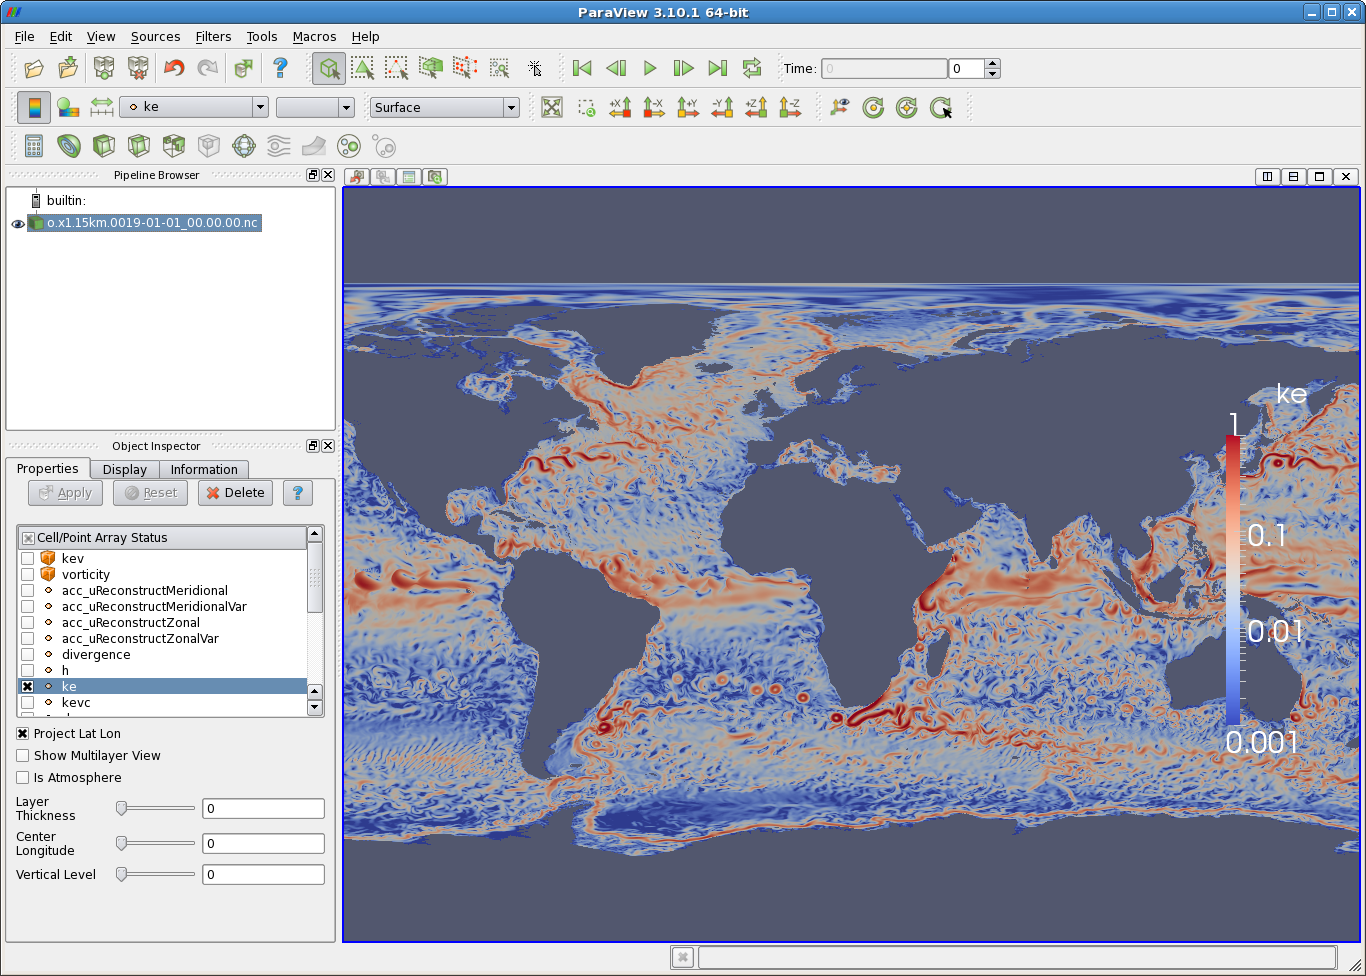
\includegraphics[width=6.5in]{shared/figures/ParaviewExample.png}
\caption{Example of ParaView to view an MPAS NetCDF file.}
\label{fig:ParaviewExample}
\end{center}
\end{figure}


\part{MPAS-Ocean}
\chapter{MPAS-Albany Land Ice Introduction}
\label{chap:landice-intro}

\section{Background}

During the past decade, numerical ice sheet models (ISMs) have undergone a renaissance relative to their predecessors. This period of intense model development was initiated following the Fourth Assessment Report of the Intergovernmental Panel on Climate Change \citep{IPCCWG1PhysicalSolomon2007}, which pointed to deficiencies in ISMs of the time as being the single largest shortcoming with respect to the scientific community's ability to project future sea-level rise stemming from ice sheets. 
Model maturation during this period, which continued through the IPCC's Fifth Assessment Report \citep{IPCCWG1PhysicalStocker2013} and to the present day, has focused on improvements to ISM ``dynamical cores'' (including the fidelity, discretization, and solution methods for the governing conservation equations \citep[e.g.,][]{Bueler2009,Schoof2010,Goldberg2011a,perego2012,Leng2012,Larour2012,Aschwanden2012,Cornford2013,gagliardini2013,brinkerhoff2013}), ISM model ``physics'' (for example, the addition of improved models of basal sliding coupled to explicit subglacial hydrology \citep[e.g.,][]{Schoof2005,Werder2013,Hewitt2013,Hoffman2014,Bueler2015}; and ice damage, fracture, and calving \citep[e.g.,][]{Astrom2014,Bassis2015,Borstad2016,Jimenez2017}) and the coupling between ISMs and Earth System Models (ESMs) \citep[e.g.,][]{Ridley2005,vizcaino2008,Vizcaino2009,Fyke2011,Lipscomb2013}. These ``next generation'' ISMs have been applied to community-wide experiments focused on assessing (i) the sensitivity of ISMs to idealized and realistic boundary conditions and environmental forcing and (ii) the potential future contributions of ice sheets to sea-level rise \citep[see e.g.,][]{pattyn2013,Nowicki2013a,Nowicki2013b,Bindschadler2013,Shannon2013,edwards2014}. 

While these efforts represent significant steps forward, next-generation ISMs continue to confront new challenges. These come about as a result of (1) applying ISMs to larger (whole-ice sheet), higher-resolution (regionally $O$(1 km) or less), and more realistic problems, (2) adding new or improved sub-models of critical physical processes to ISMs, and (3) applying ISMs as partially or fully coupled components of ESMs. The first two challenges relate to maintaining adequate performance and robustness, as increased resolution and/or complexity have the potential to increase forward model cost and/or degrade solver reliability. The latter challenge relates to the added complexity and cost associated with optimization workflows, which are necessary for obtaining model initial conditions that are realistic and compatible with forcing from ESMs. %(See related discussion in \cite{perego2014}). 
These challenges argue for ISM development that specifically targets the following model features and capabilities: 
\begin{enumerate}

\item parallel, scalable, and robust, linear and nonlinear solvers

\item variable and / or adaptive mesh resolution 

\item computational kernels based on flexible programming models, to allow for implementation on a range of High-Performance Computing (HPC) architectures\footnote{For example, traditional CPU-only architectures and MPI programming models versus CPU+GPU, hybrid architectures using MPI for nodal communication and OpenMP or CUDA for on-node parallelism.}

\item adjoint capabilities for use in high-dimensional parameter field optimization and uncertainty quantification 

\end{enumerate}

Based on these considerations, we have developed MPAS-Albany Land Ice (MALI), which is composed of three major components: 
1) model framework, 2) dynamical cores for solving equations of conservation of momentum, mass, and energy, and 3) modules for additional model physics. The model leverages existing and mature frameworks and libraries, namely the Model for Prediction Across Scales (MPAS) framework and the Albany and Trilinos solver libraries. These have allowed us to take into consideration and address, from the start, many of the challenges discussed above.
The model is described in detail in the following sections.  
MPAS-Albany Land Ice is described by a model description paper currently in review in Geoscientific Model Descriptions at:
\url{https://www.geosci-model-dev-discuss.net/gmd-2018-78/}
Much of the information in this User's Guide is derived from the text of that paper.
The User's Guide is further updated at the model evolves.


\section{MALI Meshes}

MALI typically uses centroidal Voronoi meshes on a plane.  
Spherical Voronoi meshes can also be used, but little work has been done with such meshes to date. 
Tools for creating and manipulating meshes are not yet publicly available.
MALI employs a C-grid discretization \citep{Arakawa1977} for advection, meaning state variables (ice thickness and tracer values) are located at Voronoi cell centers,
and flow variables (transport velocity, $u_n$) are located at cell edge midpoints (Figure \ref{fig:cellDiagram}).
MALI uses a sigma vertical coordinate (specified number of layers, each with a spatially uniform layer thickness fraction, see \citep{Petersen2015} for more information):
\begin{equation}
\sigma = \frac{s-z}{H}
\label{eq:sigma}
\end{equation}
where $s$ is surface elevation, $H$ is ice thickness, and $z$ is the vertical coordinate. 
Table \ref{table:meshes} describes the relationship between the MPAS Voronoi grid and the Delaunay Triangulation used by the Albany First Order velocity solver.

\begin{figure}[h]
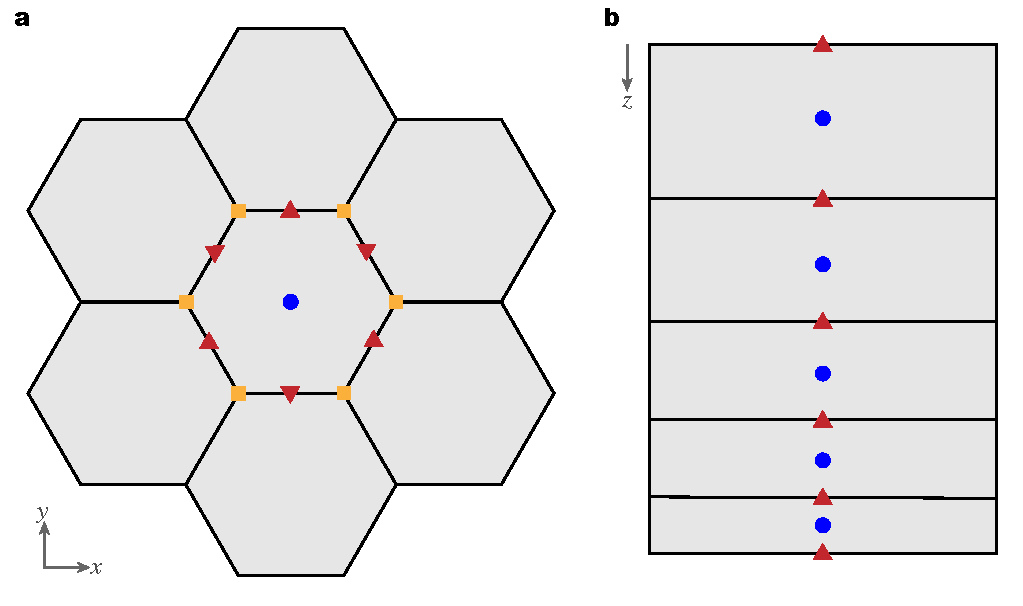
\includegraphics[width=8.3cm]{landice/figures/mpas_grids.pdf}
\caption{MALI grids.  
a) Horizontal grid with cell center (blue circles), edge midpoint (red triangles), and vertices (orange squares) identified for the center cell. Scalar fields ($H$, $T$) are located at cell centers.  Advective velocities ($u_n$) and fluxes are located at cell edges.
b) Vertical grid with layer midpoints (blue circles) and layer interfaces (red triangles) identified.  
Scalar fields ($H$, $T$) are located at layer midpoints.  Fluxes are located at layer interfaces.
}
\label{fig:cellDiagram}
\end{figure}


\begin{table*}[h]
\caption{Correspondence between the MPAS Voronoi tesselation and its dual Delaunay triangulation used by Albany.
Key MALI model variables that are natively found at each location are listed.  Note that variables are interpolated from 
one location to another as required for various calculations.
}
\begin{tabular}{lll}
\hline
Voronoi tesselation & Delaunay triangulation & Variables\\
\hline
cell center & triangle node   & $H, T, u, v$, $\Phi$ (MPAS) \\
cell edge   & triangle edge   & $u_n$ (for advection) \\
cell vertex & triangle center & $\Phi$ (Albany)\\
\hline
\end{tabular}
\label{table:meshes}
\end{table*}




\section{Albany velocity solver}
MPAS-Albany Land Ice can optionally be compiled with support for the Albany First Order velocity solver.
Albany is an open source, C++ multi-physics code base for the solution and analysis of coupled systems of partial-differential equations (PDEs) \citep{Salinger2016}. 
It is a finite element code that can (in three spatial dimensions) employ unstructured meshed comprised of hexahedral, tetrahedral, or prismatic elements. 
Albany is designed to take advantage of the computational mathematics tools available within the Trilinos suite of software libraries \citep{Trilinos} 
and it uses template-based generic programming methods to provide extensibility and flexibility \citep{Pawlowski2012}. 
Together, Albany and Trilinos provide parallel data structures and I/O, discretization and integration algorithms, 
linear solvers and preconditioners, nonlinear solvers, continuation algorithms, and tools for automatic differentiation (AD) and optimization. 
By formulating a system of equations in the residual form, Albany employs AD to automatically compute the Jacobian matrix, 
as well as forward and adjoint sensitivities. 
Albany can solve large-scale PDE-constrained optimization problems, using Trilinos optimization package ROL, 
and it provides uncertainty quantification capabilities through the Dakota framework \citep{Adams2013}. 
It is a massively parallel code by design and recently it has been adopting the Kokkos \citep{kokkos2014} programming model 
to provide manycore performance portability \citep{demeshko2018} on major HPC platforms. 
Albany provides several applications including LCM (Laboratory for Computational Mechanics) for solid mechanics problems, 
QCAD (Quantum Computer Aided Design) for quantum device modeling, and LI (Land Ice) for modeling ice sheet flow. 
We refer to the code that discretizes these ice sheet diagnostic momentum balance equations as Albany-LI.
Albany-LI was formerly known as Albany/FELIX (Finite Elements for Land Ice eXperiments), and described by 
\cite{tezaur2015a,tezaur2015b} and \cite{Tuminaro2016} under that name.

To compile MALI with support for Albany capabilities requires an installation of the Albany libraries.
Installations exist on many Department of Energy supercomputers.
To build them yourself, review the information at \url{https://github.com/gahansen/Albany/wiki}.
Compiling Albany requires a build of Trilinosi (\url{https://github.com/trilinos/Trilinos}) with specific packages and third party libraries,
and is not a trivial exercise.
Compiling Albany for usage with MPAS requires setting the Albany cmake configuration variable {\tt ENABLE\_MPAS\_INTERFACE:BOOL=ON}.
A successful Albany installation will include the file {\tt export\_albany.in}.  
Before compiling MPAS, the environment variable {\tt MPAS\_EXTERNAL\_LIBS} should be set to the list of libraries listed in this file.
Then, MALI with Albany support is enabled by compiling with {\tt ALBANY=true}, e.g.:

{\tt make gfortran CORE=landice ALBANY=true}

For MALI runs using the Albany velocity solver ({\tt config\_velocity\_solver='FO'}), an Albany .xml configuration file named {\tt albany\_input.xml}
is required in addition to the standard MPAS namelist and streams configuration files.
Examples of that file exist in the MPAS repository within subdirectories for various tests in the {\tt testing\_and\_setup/compass/landice} directory.
For further details on compiling Albany and configuring run-time options for Albany, see  \url{https://github.com/gahansen/Albany}.


% Grid generation is not included in MPAS release 1.0.
% In a future release, describe here ocean-specific grid
% generation, currently the basin.F program.
%\appendix{Generating meshes}
\label{chap:mpas_grid_generation}

This chapter describes the steps used to create the  spherical centroidal Voronoi tessellation (SCVT) meshes and mesh-decomposition files used by MPAS models.
Since it can take considerable time (often several days or more) to generate a mesh as described in \S \ref{sec:global_scvt}, it is recommended to obtain 
and use existing SCVT meshes from \url{http://www.mmm.ucar.edu/people/duda/mpas/} whenever possible; these meshes can be quickly
modified to shift or rotate the refinement regions over the geographic areas of interest using the utility program described in \S \ref{sec:grid_rotate}.

\section{Density functions}

In all MPAS models, the horizontal meshes are SCVTs with a C-grid staggering of
velocities. As their name suggests, SCVTs are Voronoi tessellations defined on the surface of a sphere, and in which the generating 
point for each Voronoi region is also the mass centroid of that region with respect to some {\em density function}. An overview of
the application of SCVTs to multi-resolution climate modeling is given in Ringler et al. (2008)
\footnote{Ringler, T., L. Ju and M. Gunzburger, 2008, A multiresolution method for climate system modeling: application of spherical centroidal Voronoi tessellations, {\em Ocean Dynamics}, 58 (5-6), 475-498. doi:10.1007/s10236-008-0157-2.}.

For the purposes of generating SCVTs, the central concern lies with the density function, $\rho$, which is a user-defined
function relating the relative resolutions in different regions of the mesh. Specifically, for two generating points of the 
SCVT, ${\bf x}_i$ and ${\bf x}_j$,
\[
{h_i \over h_j} \approx \left({\rho({\bf x}_j) \over \rho({\bf x}_i)} \right)^{1 \over 4},
\]
where $h_i$ and $h_j$ are the diameters of the Voronoi cells associated with ${\bf x}_i$ and ${\bf x}_j$, respectively.

In the mesh generation program global\_scvt, described in the next section, the density function is defined programatically in the Fortran function
{\tt density\_for\_point()}, which returns the value of the density function, $\rho({\bf x})$, given a location on the sphere, ${\bf x}$.
   
\section{The global\_scvt program}
\label{sec:global_scvt}

\subsection{Compilation}
                                                                                             
As a first step toward building the global\_scvt code, the environment variable                     
{\tt NETCDF} must be set to the root of the netCDF installation. Unlike with the MPAS model, separate make targets are not
defined for each compiler set, and it will generally be necessary to edit the top-level Makefile to set the compiler and compiler flags                 
that will be used to build global\_scvt; however, there are commented-out sections in the Makefile for using either of the ifort, pgf90, or gfortran compilers that may be uncommented or used as a starting point for other compilers. Also, if the netCDF installation has a separate Fortran interface library, {\tt -lnetcdff} will need to be added before {\tt -lnetcdf} in the Makefile. The global\_scvt program is parallelized with OpenMP, so if compiler support is available, OpenMP compiler flags may be added
in the Makefile as well.                      

Before compiling the global\_scvt program, a density function should first be defined in the function {\tt density\_for\_point()} in {\tt src/module\_scvt.F}. The default density function is a uniform density function that returns a value of 1.0 for all locations
on the sphere, and commented code in {\tt density\_for\_point()} may be uncommented to achieve an area of circular refinement. {\em Note that, although $\rho({\bf x})$ could in principle take on any non-negative value, the code to scale eddy viscosities by the mesh resolution in the MPAS model assumes that $\rho({\bf x}) \in (0,1]$, so care should be taken when designing a new density function: a value of 1.0 should correspond to the highest-resolution regions(s) in the mesh.}                                      
                                                                                                
After editing the Makefile and defining the desired density function, running `make' should create the grid\_gen executable 
in the top-level directory. A second program, grid\_ref, may also be created, but this program is not needed by the current version 
of the global\_scvt program.

\subsection{Running}

As will be described in Section \ref{sec:grid_gen_efficiency}, a typical mesh is generated using multiple refinement steps. Within each of these steps, an SCVT with a fixed
number of generating points is converged before the SCVT is refined, giving a larger number of generating points to begin the next step. In this section, the process of converging an SCVT within a single step is described.

Two files are needed in order to run the grid\_gen program: an initial generating point file, {\tt locs.dat}, and a                        
namelist file, {\tt namelist.input}. The {\tt locs.dat} file contains a list of the Cartesian coordinates (assuming a unit-radius sphere
centered at the origin) of each of the beginning generating points, and the {\tt namelist.input} file specifies the number of generating points to be read from the {\tt locs.dat} file, the number of iterations to run, and the convergence criteria; a complete list of namelist variables is provided in the table below.

\vspace{12pt}
\begin{longtable}{|p{1.25in} |p{4.5in}|}
\hline
np & the number of points to read from the {\tt locs.dat} file \\ \hline
locs\_as\_xyz & whether the initial generating points in {\tt locs.dat} are given in Cartesian space ({\tt .true.}) or latitude-longitude space ({\tt .false.}) \\ \hline
n\_scvt\_iterations & the maximum number of Lloyd iterations to perform \\ \hline
eps & the convergence criterion, specifying the maximum permissible average movement of a generating point during an iteration \\ \hline
l2\_conv & whether to stop iterating if the convergence criterion is met \\ \hline
inf\_conv & currently the same meaning as l2\_conv \\ \hline
min\_dx & the targeted minimum grid distance in the mesh, on which an estimate for the number of generating points will be based; see Section \ref{sec:estimating_np} \\ \hline
\end{longtable}
\vspace{12pt}

\noindent A convergence criterion of $1\times10^{-10}$ should be sufficient, and in                     
practice, many thousands of iterations are needed to reach this tolerance.

If grid\_gen was compiled with OpenMP support, the environment variable {\tt OMP\_NUM\_THREADS} can be set to the 
number of threads that will be used by the program. Then, grid\_gen can be run with no command-line arguments:

\vspace{12pt}
{\tt > ./grid\_gen}
\vspace{12pt}
                                                                                         
                                                                                                
When grid\_gen finishes --- either because the convergence criterion has been met, or the
maximum number of iterations have been performed ---  several output files should be created: 

\begin{itemize}
\item {\tt scvt\_initial.ps} --- a plot of the mesh at the start of iterations,
\item {\tt scvt\_final.ps} --- a plot of the mesh after iterations,
\item {\tt grid.nc} --- the actual MPAS mesh file, which can be used with the initialization core to create an MPAS input file,
\item {\tt graph.info} --- information describing the cell connectivity graph of the mesh, to be used with a graph partitioner as described in Section \ref{sec:metis}, and
\item {\tt locs.dat.out} --- a list of the final generating points appended with a set of $3 np - 6$ refinement points. 
\end{itemize}

If the tolerance specified in the {\tt namelist.input} file was met, the SCVT mesh should be sufficiently converged, and the resulting {\tt grid.nc}
file can be used with the initialization program to create an initial condition file for MPAS; alternatively, the full set of $4 np - 6$ refinement points in 
the {\tt locs.dat.out} file can be used as input to the grid\_gen program to create another SCVT with approximately twice the resolution. If, however, the specified tolerance was not met, the {\tt locs.dat.out} file may be copied to {\tt locs.dat}, and further iteration may be performed on the SCVT.

To create a plot of the mesh with coastlines, which can be helpful when locating or sizing refinement regions, the {\tt mesh.ncl} script may be used to plot the mesh directly from                 
the {\tt grid.nc} file.                                                                          

\subsection{Estimating the required number of generating points}
\label{sec:estimating_np}

Setting the {\tt min\_dx} variable in the {\tt namelist.input} file to the targeted minimum grid distance in the mesh and running the grid\_gen program will cause the program to print out an estimate for the number of generating points that will be required to achieve that minimum grid distance with the density function provided in {\tt density\_for\_point()}.

\subsection{Efficiency concerns}
\label{sec:grid_gen_efficiency}

Although one could, given an estimate for the number of generating points needed to achieve the required absolute resolutions in the mesh,
create a {\tt locs.dat} file with that number of randomly chosen points on the unit sphere, and, using that {\tt locs.dat} file, converge a final SCVT, 
experience indicates that a stepwise approach can significantly reduce the required wallclock time.                   

   
\section{The grid\_rotate program} 
\label{sec:grid_rotate} 

The purpose of the grid\_rotate program is simply to rotate an MPAS mesh file, moving a refinement region from one geographic location to another, so that the mesh can be re-used for different applications. This utility was developed out of the need to save computational resources, since generating an SCVT --- particularly one with a large number of generating points or a high degree of refinement --- can take considerable time.

To build the grid\_rotate program, the Makefile should first be edited to set the Fortran compiler to be used; if the netCDF installation pointed to by the {\tt NETCDF} environment variable was build with a separate Fortran interface library, it will also be necessary to add {\tt -lnetcdff} just before {\tt -lnetcdf} in the Makefile. After editing the Makefile, running `make' should result in a grid\_rotate executable file.

Besides the MPAS grid file to be rotated, grid\_rotate requires a namelist file, {\tt namelist.input}, which specifies the rotation to be applied to the mesh. The namelist variables are summarized in the table below
   
\vspace{12pt}
\begin{longtable}{|p{3.25in} |p{2.5in}|}
\hline
config\_original\_latitude\_degrees & original latitude of any point on the sphere \\ \hline
config\_original\_longitude\_degrees & original longitude of any point on the sphere \\ \hline
config\_new\_latitude\_degrees &  latitude to which the original point should be shifted \\ \hline
config\_new\_longitude\_degrees &  longitude to which the original point should be shifted \\ \hline
config\_birdseye\_rotation\_counter\_clockwise\_degrees & rotation about a vector from the sphere center through the original point \\ \hline
\end{longtable}
\vspace{12pt}

\noindent Essentially, one chooses any point on the sphere, decides where that point should be shifted to,
and specifies any change to the orientation (i.e., rotation) of the mesh about that point. 

Having set the rotation parameters in the {\tt namelist.input} file, the grid\_rotate program should be run with two command-line options
specifying the original grid file name and the name of the rotated grid file to be produced, e.g.,

\vspace{12pt}
{\tt > grid\_rotate grid.nc grid\_SE\_Asia\_refinement.nc}
\vspace{12pt}

The original grid file will not be altered, and a new, rotated grid file will be created. The NCL script {\tt mesh.ncl} may be used to plot either of the original or rotated grid files after suitable setting the name of the grid file in the script.
   
   
\section{Graph partitioning with METIS} 
\label{sec:metis}

{\color{red} THIS SECTION WAS COPIED TO mpas_build_instructions.tex  FOR RELEASE 1.0. WHEN GRID GENERATION IS INCLUDED, DELETE THE METIS SECTION FROM mpas_build_instructions.tex}.

Before MPAS can be run in parallel, a mesh decomposition file with an appropriate number of 
partitions (equal to the number of MPI tasks that will be used) is required in the run directory.  A limited number of mesh decomposition files ({\tt graph.info.part.*}) are provided with each test case (see Test Cases Chapter).  In order to create new mesh decomposition files for your desired number of partitions, begin with the {\tt graph.info} file created by the grid\_gen program or available with your test case, and partition with METIS software (\url{http://glaros.dtc.umn.edu/gkhome/views/metis}). The serial graph partitioning program, METIS (rather than ParMETIS or hMETIS) should be sufficient for quickly partitioning any SCVT produced by the grid\_gen mesh generator.

After installing METIS, a {\tt graph.info} file may be partitioned into $N$ partitions by running

\vspace{12pt}
{\tt > gpmetis graph.info} $N$
\vspace{12pt}

\noindent The resulting file, {\tt graph.info.part.}$N$, can then be copied into the MPAS run directory
before running the model with $N$ MPI tasks.



\chapter{Forward Mode}
\label{chap:forward_mode}
\newcommand{\mode}{forward}
\section{Purpose}
\label{sec:forward_purpose}

The MPAS-Ocean model may be compiled in two modes, forward (this chapter) and analysis (chapter \ref{chap:analysis_mode}).  Forward mode is the typical configuration for an ocean model, where the model is initialized at start-up, steps forward through time, and periodically writes output and restart files to disk.  Namelist options for forward mode are set in the namelist.ocean\_forward file in the run directory.  The user may specify any number of output streams, each with a list of variables and write frequency, in the streams.ocean\_forward file.  Analysis members are available for computation and i/o in forward mode.  For example, see global\_stats under Namelist Options.  

\section{Compilation}
\label{sec:forward_compilation}

In order to build the ocean core in forward mode, one must first select a build
target. In this example, we'll build using the gfortran build target. The build
enviroment should be setup as described in Chapter
\ref{chap:mpas_build_instructions}. After the build environment and target are
selected, the forward mode of the ocean core can be built as follows:

\vspace{12pt}
{\tt > make gfortran CORE=ocean MODE=forward}


\section{Dimensions}
\label{sec:forward_dimensions}
{\small
\begin{center}
\begin{longtable}{| p{1.2in} || p{1.0in} | p{4.0in} |}
	\hline 
	{\bf Name} & {\bf Units} & {\bf Description} \endfirsthead
	\hline 
	{\bf Name} & {\bf Units} & {\bf Description} (Continued) \endhead
	\hline 
	\hline 
	nCells & $unitless$ & The number of polygons in the primary grid. \\ 
	\hline
	nEdges & $unitless$ & The number of edge midpoints in either the primary or dual grid. \\ 
	\hline
	maxEdges & $unitless$ & The largest number of edges any polygon within the grid has. \\ 
	\hline
	maxEdges2 & $unitless$ & Two times the largest number of edges any polygon within the grid has. \\ 
	\hline
	nAdvectionCells & $unitless$ & The largest number of advection cells for any edge. \\ 
	\hline
	nVertices & $unitless$ & The total number of cells in the dual grid. Also the number of corners in the primary grid. \\ 
	\hline
	TWO & $unitless$ & The number two as a dimension. \\ 
	\hline
	R3 & $unitless$ & The number three as a dimension. \\ 
	\hline
	SIX & $unitless$ & The number six as a dimension. \\ 
	\hline
	FIFTEEN & $unitless$ & The number 15 as a dimension. \\ 
	\hline
	TWENTYONE & $unitless$ & The number 21 as a dimension. \\ 
	\hline
	vertexDegree & $unitless$ & The number of cells or edges touching each vertex. \\ 
	\hline
	nVertLevels & $unitless$ & The number of levels in the vertical direction. All vertical levels share the same horizontal locations. \\ 
	\hline
	nVertLevelsP1 & $unitless$ & The number of interfaces in the vertical direction. \\ 
	\hline
	nZonalMeanBins & $unitless$ & Maximum number of bins for zonal mean. \\ 
	\hline
	nZonalMeanBinsP1 & $unitless$ & Maximum number of bins for zonal mean, plus one. \\ 
	\hline
\end{longtable}
\end{center}
}
\section[Namelist options]{\hyperref[chap:namelist_sections]{Namelist options}}
\label{sec:forward_namelist_tables}
Embedded links point to more detailed namelist information in the appendix.
\subsection[time\_management]{time\_management}
\label{subsec:forward_nm_tab_time_management}
General time management is handled by the time\_management namelist record.
Included options handle time-related parts of MPAS, such as the calendar and if the simulation is a restart or not.

Users should use this record to specify the beginning time of the simulation,
and either the duration or the end of the simulation. Only the end or the
duration need to be specified as the other is derived within MPAS from the
beginning time and other specified one.

{\bf TBA: If both duration and stop are specified, then what happens?)}

\vspace{0.5in}
{\small
\begin{center}
\begin{longtable}{| p{2.0in} || p{4.0in} |}
	\hline
	{\bf Name} & {\bf Description} \endfirsthead
	\hline 
	{\bf Name} & {\bf Description} (Continued) \endhead
	\hline
	\hline
	\hyperref[sec:nm_sec_config_do_restart]{config\_do\_restart} & Determines if the initial conditions should be read from a restart file, or an input file. \\
	\hline
	\hyperref[sec:nm_sec_config_start_time]{config\_start\_time} & Timestamp describing the initial time of the simulation. If it is set to 'file', the initial time is read from restart\_timestamp. \\
	\hline
	\hyperref[sec:nm_sec_config_stop_time]{config\_stop\_time} & Timestamp descriping the final time of the simulation. If it is set to 'none' the final time is determined from config\_start\_time and config\_run\_duration. \\
	\hline
	\hyperref[sec:nm_sec_config_run_duration]{config\_run\_duration} & Timestamp describing the length of the simulation. If it is set to 'none' the duration is determined from config\_start\_time and config\_stop\_time. config\_run\_duration overrides inconsistent values of config\_stop\_time. \\
	\hline
	\hyperref[sec:nm_sec_config_calendar_type]{config\_calendar\_type} & Selection of the type of calendar that should be used in the simulation. \\
	\hline
\end{longtable}
\end{center}
}
\subsection[io]{io}
\label{subsec:forward_nm_tab_io}
The io namelist record provides options for modifications to the I/O system of
MPAS. These include frequency, file name, and parallelization options.

\vspace{0.5in}
{\small
\begin{center}
\begin{longtable}{| p{2.0in} || p{4.0in} |}
	\hline
	{\bf Name} & {\bf Description} \endfirsthead
	\hline 
	{\bf Name} & {\bf Description} (Continued) \endhead
	\hline
	\hline
	\hyperref[sec:nm_sec_config_stats_interval]{config\_stats\_interval} & Timestamp determining how often a global statistics files should be written. \\
	\hline
	\hyperref[sec:nm_sec_config_write_stats_on_startup]{config\_write\_stats\_on\_startup} & Logical flag determining if statistics files should be written prior to the first time step. \\
	\hline
	\hyperref[sec:nm_sec_config_write_output_on_startup]{config\_write\_output\_on\_startu-}\hyperref[sec:nm_sec_config_write_output_on_startup]{p}& Logical flag determining if an output file should be written prior to the first time step. \\
	\hline
	\hyperref[sec:nm_sec_config_pio_num_iotasks]{config\_pio\_num\_iotasks} & Integer specifying how many IO tasks should be used within the PIO library. A value of 0 causes all MPI tasks to also be IO tasks. IO tasks are requried to write contiguous blocks of data to a file. \\
	\hline
	\hyperref[sec:nm_sec_config_pio_stride]{config\_pio\_stride} & Integer specifying the stride of each IO task. \\
	\hline
\end{longtable}
\end{center}
}
\subsection[time\_integration]{time\_integration}
\label{subsec:forward_nm_tab_time_integration}
The time integration namelist controls parameters that pertain to all time-stepping methods.  At present, Forward Euler is the only time integration method implemented.

\vspace{0.5in}
{\small
\begin{center}
\begin{longtable}{| p{2.0in} || p{4.0in} |}
	\hline
	{\bf Name} & {\bf Description} \endfirsthead
	\hline 
	{\bf Name} & {\bf Description} (Continued) \endhead
	\hline
	\hline
	\hyperref[sec:nm_sec_config_dt]{config\_dt} & Length of model time-step. \\
	\hline
	\hyperref[sec:nm_sec_config_time_integrator]{config\_time\_integrator} & Time integration method. \\
	\hline
\end{longtable}
\end{center}
}
\subsection[ALE\_vertical\_grid]{ALE\_vertical\_grid}
\label{subsec:forward_nm_tab_ALE_vertical_grid}
The MPAS-Ocean vertical grid is structured arbitrary Lagrangian-Eulerian (ALE).   ALE provides a great deal of freedom in the choice of vertical coordinate: when fully Eulerian, MPAS-Ocean is a z-level model with fixed thicknesses; when fully Lagrangian, there is no vertical transport between layers, and layers expand and contract like an isopycnal ocean model.  In between are many additional options, such as z-star where layers expand in proportion to the sea surface height, and sigma, where coordinates are terrain-following.

MPAS-Ocean employs the continuity equation,
\begin{eqnarray}
\label{ocean:continuity thickness}
\frac{\partial h_{k}}{\partial t} + D_k + w^t_k - w^t_{k+1} =0
\end{eqnarray}
for the ALE formulation, where variables are defined in Table \ref{oceanTable:ALE_variables}.  The ALE algorithm is as follows:
\begin{enumerate}
\item ALE step: Compute desired thickness for the new time,
\begin{eqnarray}
\label{ocean:desired thickness}
h_k^{ALE} = h_k^{rest} + h_k^{SSH} + h_k^{hf} + h_k^{min}
\end{eqnarray}
\item ALE step: Solve for vertical transport $w^t$ from (\ref{ocean:continuity thickness}),
\begin{eqnarray}
\label{ocean:vert tranport}
w^t_k = w^t_{k+1} - D_k - \frac{h^{ALE}_k - h^n_k}{\Delta t}
\end{eqnarray}
\item Solve for new thickness, $h_{k}^{n+1}$, using the continuity equation (\ref{ocean:continuity thickness}) within the time integration routine.
\end{enumerate}
The redundancy in steps 2 and 3 are intentional, so that step 2 is isolated within the ALE subroutine, and step 3 is solved in the timestepping subroutine in the identical manner as the tracer equation (\ref{ocean:tracer}).

The desired ALE thickness includes contributions from four terms (\ref{ocean:desired thickness}):
\begin{enumerate}
\item {\bf Resting thickness}, $h^{rest}$, is the layer thickness when the ocean is at rest, i.e. without SSH or internal perturbations.  For z-type coordinates, the resting thickness is constant in each horizontal layer.
\item {\bf SSH alteration}, $h^{SSH}$, alters layer thicknesses so that they change in proportion to the sea surface height (SSH),
\begin{eqnarray}
\label{ocean:h ssh}
   h_k^{SSH} =  \zeta \frac{W_k h^{rest}_k}{\sum_{k'=1}^{kmax}W_{k'}h^{rest}_{k'}}
\end{eqnarray}
The weights $W_k$ determine how SSH oscillations are distributed amongst the layers, as described in Table \ref{oceanTable:vertical coordinates}.
\item {\bf High-frequency thickness}, $h^{hf}$, allows high-frequency thickness oscillations, such as internal gravity waves, to be treated in a Lagrangian manner.  This is the ``z-tilde'' scheme of \citet{Leclair_Madec11om} described in the next section.
\item {\bf Minimum thickness alteration}, $h^{min}$, is the change in thickness required to enforce the minimum thickness in each cell.  When a cell is too thin, $h^{min}$ is positive, while nearby cells in the vertical incur a corresponding negative $h^{min}$ to conserve volume in the column.
\end{enumerate}
Of the four terms, resting thickness is always positive, while the others are small alterations about zero.  Summing a column,
\begin{eqnarray}
\sum_{k=1}^{kmax} h_k^{ALE} &=& \sum_{k=1}^{kmax} h_k^{rest} + \sum_{k=1}^{kmax}h_k^{SSH} + \sum_{k=1}^{kmax}h_k^{hf} + \sum_{k=1}^{kmax}h_k^{min} 
\nonumber \\
&=& H + \zeta + 0 + 0.
\nonumber
\end{eqnarray}
Thus the first two terms are always included so that the column thickness sums to $H+\zeta$, while the second two terms are optional and may be turned on with flags.

In order to assist users in choosing the correct settings, we provide a description of traditional vertical coordinate names in Table \ref{oceanTable:vertical coordinates}.
The vertical coordinate type also depends upon the set-up of the layerThickness variable in the initial condition file.  For all Z-type vertical coordinates, initial layer thicknesses are horizontally constant.  For sigma coordinates, layers are terrain-following and all layers are employed.  In this case, the user may still choose amongst the flags in SSH may be distributed through the column just like with z-type models in Table \ref{oceanTable:vertical coordinates}.

In order to run an isopycnal configuration, use config\_vert\_coord\_movement='impermeable\_interfaces' and set initial temperature and salinity to be constant within each layer.  All vertical tracer diffusion must be off so that the density in each layer remains constant.  For an isopycnal set-up, the equation of state is still called at each timestep, so a linear equation of state is recommended to avoid depth-dependancy of the density.  The user may choose a Montgomery Potential (\ref{ocean:Montgomery Potential}) or standard pressure gradient (\ref{ocean:grad p}); Montgomery Potential is a more common choice for isopycnal configurations, but both are tested and functional.  MPAS-Ocean does not support massless layers at this time, so isopycnal vertical coordinates may only be used for idealized domains.

\begin{table}[ht] 
\caption{Vertical coordinate settings for traditional names.}
\vspace{0.5cm} \centering 
\begin{tabular}{c c c c c c} 
\hline\hline flag name &  {\bf Z-Level} & {\bf Z-star} & {\bf weighted Z-star} &  {\bf isopycnal}  \\
\hline 
config\_vert\_ & 'fixed' & 'uniform\_stretching' & 'user\_specified' & 'impermeable\_ \\
coord\_movement & & & & interfaces'
\\
weights & $W_k =\left\{ \begin{array}{c} 1\; k=1\\ 0\; k>1 \end{array}\right.$ & $W_k=1\;\;\forall\;\;k$ & input file & not applicable \\
\hline 
\end{tabular} \label{oceanTable:vertical coordinates} 
\end{table}

\begin{table}[h!t] 
\caption{Variables used in ALE equation sets.  Column 3 shows the native horizontal grid location.  A subscript $k$ indicates indicates the layer index.  The $\nabla$ indicates a horizontal gradient within a single layer.} 
\vspace{0.5cm} \centering 
\begin{tabular}{c c c c } 
\hline\hline symbol &  name & grid &  notes  \\
\hline 
$D$  & thickness-weighted divergence & cell & $D_k = \nabla \cdot  \left( h_k {\bf u}_k \right)$  \\ 
${\bar D}$ & barotropic divergence & cell & ${\overline D} = \sum\limits_{k=1}^{kmax} D_k$  \\ 
$D'$  & baroclinic divergence & cell & $D'_k = D_k-\frac{h_k}{H}{\bar D}$  \\ 
$D^{lf}$  & low-frequency divergence & cell & see (\ref{ocean:Dlf})  \\ 
$D^{hf}$  & high-frequency divergence & cell & $D^{hf}_k = D'_k - D^{lf}_k$  \\ 
$h$  & layer thickness & cell &   \\ 
$h^{ALE}$  & desired ALE thickness & cell & see (\ref{ocean:desired thickness})  \\ 
$h^{rest}$  & resting thickness & cell &   \\ 
$h^{SSH}$  & SSH thickness alteration & cell & see (\ref{ocean:h ssh})  \\ 
$h^{hf}$  & high-freq. thickness alteration & cell &   see (\ref{ocean:hhf})  \\ 
$h^{min}$  & minimum thickness alteration & cell &   \\ 
$H$  & total resting thickness & cell & $H= \sum\limits_{k=1}^{kmax} h_k^{rest}$  \\ 
${\bf u}$  & velocity & edge &   \\ 
$w^t$ & vertical transport & cell  & top of layer in vertical \\
$W$  & SSH thickness weights & cell &   \\ 
$\tau_{Dlf}$  & frequency filter time scale & constant &   \\ 
$\tau_{hhf}$  & restoring time scale for $h^{hf}$ & constant &   \\ 
$\kappa_{hhf}$  & $h^{hf}$ diffusion & constant &   \\ 
$\zeta$  & sea surface height & cell &  $\zeta= \sum\limits_{k=1}^{kmax} h_k^{rest} - H$  \\ 
\hline 
\end{tabular} \label{oceanTable:ALE_variables} 
\end{table}


\vspace{0.5in}
{\small
\begin{center}
\begin{longtable}{| p{2.0in} || p{4.0in} |}
	\hline
	{\bf Name} & {\bf Description} \endfirsthead
	\hline 
	{\bf Name} & {\bf Description} (Continued) \endhead
	\hline
	\hline
	\hyperref[sec:nm_sec_config_vert_coord_movement]{config\_vert\_coord\_movement} &  Determines the vertical coordinate movement type. 'uniform\_stretching' distributes SSH perturbations through all vertical levels (z-star vertical coordinate); 'fixed' places them all in the top level (z-level vertical coordinate); 'user\_specified' allows the input file to determine the distribution using the variable vertCoordMovementWeights (weighted z-star vertical coordinate); and 'impermeable\_interfaces' makes the vertical transport between layers zero, i.e.  $w^t=0$  (idealized isopycnal). \\
	\hline
	\hyperref[sec:nm_sec_config_use_min_max_thickness]{config\_use\_min\_max\_thickness} & If true, a minimum and maximum thicknesses are enforced to prevent massless and very thick layers. \\
	\hline
	\hyperref[sec:nm_sec_config_min_thickness]{config\_min\_thickness} & Minimum thickness allowed. \\
	\hline
	\hyperref[sec:nm_sec_config_max_thickness_factor]{config\_max\_thickness\_factor} &  Maximum thickness allowed. This is a factor times the resting thickness, i.e., maximum thickness = config\_max\_thickness\_factor* $h^{rest}$ . \\
	\hline
	\hyperref[sec:nm_sec_config_set_restingThickness_to_IC]{config\_set\_restingThickness\_t-}\hyperref[sec:nm_sec_config_set_restingThickness_to_IC]{o\_IC}& If true, set restingThickness to be the same as layerThickness upon start-up. This only occurs when config\_do\_restart is false, i.e. on an initial run. \\
	\hline
	\hyperref[sec:nm_sec_config_dzdk_positive]{config\_dzdk\_positive} & Determines if the positive Z axis is aligned with the positive K index direction. \\
	\hline
\end{longtable}
\end{center}
}
\subsection[ALE\_frequency\_filtered\_thickness]{ALE\_frequency\_filtered\_thickness}
\label{subsec:forward_nm_tab_ALE_frequency_filtered_thickness}
The high-frequency thickness alteration, $h^{hf}$, in (\ref{ocean:\mode_desired thickness}) allows the thicknesses to oscillate so that high-frequency motions, such as internal gravity waves, are treated in a Lagrangian manner.  Low-freqency motions, such as seasonal changes or slow motions of water masses, are treated in an Eulerian manner.  This is the ``z-tilde'' scheme of \citet{Leclair_Madec11om}, which generally reduces spurious vertical mixing and preserves water mass properties.  Two additional prognostic equations are solved when config\_use\_freq\_filtered\_thickness is true,
\begin{eqnarray}
\label{ocean:\mode_Dlf}
 & \displaystyle
  \frac{\partial D^{lf}_k}{\partial t} = - \frac{2\pi}{\tau_{Dlf}} \left( D^{lf}_k - D'_k \right), 
\\ & \displaystyle
\label{ocean:\mode_hhf}
\frac{\partial h^{hf}_k}{\partial t} =  - D^{hf}_k - \frac{2\pi}{\tau_{hhf}} h^{hf}_k + \nabla_h\cdot \left( \kappa_{hhf} \nabla_h h^{hf}_k \right) 
\end{eqnarray}
where $\tau_{Dlf}$ is the filter timescale and other variables are defined in Table \ref{oceanTable:\mode_ALE_variables}.  This may be used in addition to any of the z-type or sigma-type vertical coordinates in Table \ref{oceanTable:\mode_vertical coordinates}.  Some combination of thickness restoring and diffusion are recommended to avoid long-term drift of $h^{hf}$ away from zero.




\vspace{0.5in}
{\small
\begin{center}
\begin{longtable}{| p{2.0in} || p{4.0in} |}
	\hline
	{\bf Name} & {\bf Description} \endfirsthead
	\hline 
	{\bf Name} & {\bf Description} (Continued) \endhead
	\hline
	\hline
	\hyperref[sec:nm_sec_config_use_freq_filtered_thickness]{config\_use\_freq\_filtered\_thickn-}\hyperref[sec:nm_sec_config_use_freq_filtered_thickness]{ess}&  If true,  $h^{hf}$  is included in the desired ALE thickness, and the prognostic equations for  $D^{lf}$  and  $h^{hf}$  are integrated in the code. \\
	\hline
	\hyperref[sec:nm_sec_config_thickness_filter_timescale]{config\_thickness\_filter\_timescal-}\hyperref[sec:nm_sec_config_thickness_filter_timescale]{e}&  Filter time scale for the low-frequency baroclinic divergence,  $\tau_{Dlf}$ . \\
	\hline
	\hyperref[sec:nm_sec_config_use_highFreqThick_restore]{config\_use\_highFreqThick\_rest-}\hyperref[sec:nm_sec_config_use_highFreqThick_restore]{ore}&  If true, the high frequency thickness prognostic equation ( $h^{hf}$ ) includes term 2 on the RHS, the restoring term.  The high frequency thickness is restored to zero with time scale  $\tau_{hhf}$ . \\
	\hline
	\hyperref[sec:nm_sec_config_highFreqThick_restore_time]{config\_highFreqThick\_restore\_-}\hyperref[sec:nm_sec_config_highFreqThick_restore_time]{time}&  Restoring time scale for high-frequency thickness,  $\tau_{hhf}$ . \\
	\hline
	\hyperref[sec:nm_sec_config_use_highFreqThick_del2]{config\_use\_highFreqThick\_del2} &  If true, high frequency thickness prognostic equation ( $h^{hf}$ ) includes term 3 on the RHS, the diffusion term. \\
	\hline
	\hyperref[sec:nm_sec_config_highFreqThick_del2]{config\_highFreqThick\_del2} &  Horizonal high frequency thickness diffusion,  $\kappa_{hhf}$ . \\
	\hline
\end{longtable}
\end{center}
}
\subsection[partial\_bottom\_cells]{partial\_bottom\_cells}
\label{subsec:forward_nm_tab_partial_bottom_cells}
\documentclass[11pt]{report}

\usepackage{epsf,amsmath,amsfonts}
\usepackage{graphicx}

\setlength{\textwidth}{6.5in}
\setlength{\oddsidemargin}{0in}
\setlength{\evensidemargin}{0in}
\setlength{\textheight}{8.5in}
\setlength{\topmargin}{0in}

\begin{document}

\title{
Requirements and Design\\
Partial Bottom Cells}
\author{MPAS Development Team}

\maketitle
\tableofcontents

%-----------------------------------------------------------------------

\chapter{Summary}

Partial bottom cells (PBCs) allow bottom topography to be represented more realistically.  Currently, MPAS-Ocean only suports full ocean cells, so the bottom depth of a column is restricted to the depth of each vertical cell interface.  With partial bottom cells, the bottom depth may take on any value.  This is still a z-level-type formulation, where cells that are fully below the bottom depth are considered land cells.  The PBC formulation will work with z-level, z-star, and z-tilde formulations.

%figure template
%\begin{figure}
%  \center{\includegraphics[width=14cm]{./Figure1.pdf}}
%  \caption{A graphical representation of the discrete boundary.}
%  \label{Figure1}
%\end{figure} 

%-----------------------------------------------------------------------

\chapter{Requirements}

\section{Requirement: initial conditions with consistant variables}
Date last modified: 2012/10/15 \\
Contributors: Mark Petersen \\

The following variables must be consistent upon starting a new simulation with mpas-ocean: bottomDepth, maxLevelCell, thickness $h$, location of initial tracers in bottom cell.

\section{Requirement: horizontal advection}
Date last modified: 2012/08/01 \\
Contributors: Mark Petersen \\

Horizontal advection must take place through a thickness that accounts for the partial bottom cell at the bottom of the column.

\section{Requirement: pressure gradient}
Date last modified: 2012/08/01 \\
Contributors: Mark Petersen \\

Pressure gradients must not contain spurious effects due to the partial bottom cells.



%-----------------------------------------------------------------------

\chapter{Algorithmic Formulations}

\section{Design Solution: initial conditions with consistant variables}

Date last modified: 2012/10/15 \\
Contributors: Mark Petersen \\

The thickness variable {\tt h(k,iCell,iStep)} will continue to be the actual thickness of fluid in the cell.  
A new variable, {\tt bottomDepth(iCell)}, is the depth below the average sea surface height ($z=0$) in each cell, and is a positive number.    The variable {\tt maxLevelCell(iCell)} is an integer of the deepest active (water-filled) cell, and {\tt refBottomDepth(k)} is the depth of the bottom of each cell in z-level coordinates.  Note that depth variables are positive, $z$ variables are negative and decrease with greater depths, and the $k$ index increases with greater depth.

In generating the initial conditions (IC), the following steps are taken:
\begin{enumerate}
\item An additional parameter, {\tt max\_partial\_bottom\_cell}, may be set between zero and one, with default .95, in the initial condition generation.  Then {\tt bottomDepth} must be altered so that a partial bottom cell has a maximum of (say) 95\% land.  This parameter may be adjusted after testing. 
\item The thickness {\tt h} at {\tt k=maxLevelCell} is reduced to take into account the thickness removed by the partial bottom cell.
\item Initial tracer values in the bottom cell are interpolated to the center of the pbc, rather than the center of the full cell.
\item Check that {\tt bottomDepth} corresponds to {\tt maxLevelCell} (because they are redundant):\\
when {\tt k=maxLevelCell(iCell)}:\\
{\tt refBottomDepth(k)<bottomDepth(iCell)< refBottomDepth(k-1)}
\end{enumerate}

The ICs could be altered in basin.F or upon start-up with mpas.  We chose to alter the ICs in mpas to reduce the number and IC files and the complexity of IC generation.  The initial netcdf file (ocean.nc, produced by basin), include a realistic
 bottomDepth variable and thickness and tracer variables for full thickness cells.

Upon start-up with {\tt config\_do\_restart = .false.}, ICs are altered as described above.  An additional flag is used as follows:
\begin{itemize}
\item If running with pbcs, set {\tt config\_alter\_ICs\_for\_pbc='zlevel\_pbcs\_on'}. Then thin pbc cells
   will be changed, and thickness and tracers will be altered to match the pbcs (steps 1-3, above).
\item If running without pbcs, set {\tt config\_alter\_ICs\_for\_pbc='zlevel\_pbcs\_off'}. Then 
   bottomDepth will be altered so it is full cells everywhere.
   If your input file does not include bottomDepth, the false option will
   initialize bottomDepth correctly for a non-pbc run.
\item Set {\tt config\_alter\_ICs\_for\_pbc='no'} for isopycnal or sigma coordinates.
\end{itemize}

Consistency between {\tt bottomDepth} and {\tt maxLevelCell} is verified afterwards if {\tt config\_check\_zlevel\_consistency=.true.}


\section{Design Solution: horizontal advection}
Date last modified: 2012/08/01 \\
Contributors: Mark Petersen \\

{\bf Option 1: Do nothing (this option was chosen)}\\

If nothing is changed in the current code, {\tt h\_edge} is computed from from the thickness of nearby cells, regardless of PBCs in the bottom layer.  This is a clean and simple solution, but if PBCs are very thin, a cell could be evacuated of water.\\

{\bf Option 2: h\_edge is limited by minimum depth of neighboring cells}\\

In POP, the thickness of a U-cell is the minimum of the four surrounding T-Cells.  Likewise in MPAS-Ocean, one could compute the edge thickness using the minimum bottom depth of the two surrounding cells.  For the computation of {\tt h\_edge} using higher order advection methods, this will require further thought.

\section{Design Solution: pressure gradient}
Date last modified: 2012/08/01 \\
Contributors: Mark Petersen \\

{\bf Option 1: Do nothing (this option was chosen)}\\

MPAS-Ocean currently has two terms related to the pressure gradient,
\begin{equation}
- \frac{1}{\rho_0}\nabla p_k  - \frac{\rho g}{\rho_0}\nabla z^{mid}_k.
\end{equation}
where the gradient of $z^{mid}$ makes up pressure differences due to tilted levels.  However, in a stratified ocean, pressure gradient errors occur when the tilting of levels is large.  In a z-star system without PBCs, these perturbations are limited by the ratio of sea surface height to total depth, so only a few percent.  With the inclusion of PBCs, $z^{mid}$ could vary from one gridcell to the next by half the layer thickness.\\

{\bf Option 2: Interpolate T \& S to center of bottom cell for pressure computation}\\

If the pressure gradient errors are deemed to be too large, one could extrapolate the temperature and salinity values to the mid-depth of the bottom cell, and compute density and pressure at that location.  This will require a special case when {\tt k=maxLevelCell}.  There will need to be an extra case in the computation of $\nabla z^{mid}$ as well, so that $z^{mid}$ at the bottom cell is at the cell center.


%-----------------------------------------------------------------------

\chapter{Design and Implementation}

\section{Implementation: consistency between thickness and partial bottom cell variables}
Date last modified: 2012/08/01 \\
Contributors: Mark Petersen \\


\section{Implementation: horizontal advection}
Date last modified: 2012/08/01 \\
Contributors: Mark Petersen \\


\section{Implementation: pressure gradient}
Date last modified: 2012/08/01 \\
Contributors: Mark Petersen \\


%-----------------------------------------------------------------------

\chapter{Testing}

\section{Testing and Validation: Partial bottom cells}
Date last modified: 2012/08/01 \\
Contributors: Mark Petersen \\

Use the test problem, already in the repository, following Ilicak ea 2012 overflow test case (\#4).


%-----------------------------------------------------------------------

\end{document}

\vspace{0.5in}
{\small
\begin{center}
\begin{longtable}{| p{2.0in} || p{4.0in} |}
	\hline
	{\bf Name} & {\bf Description} \endfirsthead
	\hline 
	{\bf Name} & {\bf Description} (Continued) \endhead
	\hline
	\hline
	\hyperref[sec:nm_sec_config_alter_ICs_for_pbcs]{config\_alter\_ICs\_for\_pbcs} & If true, initial conditions are altered according to the config\_pbc\_alteration\_type flag. The alteration of layer thickness only occurs when config\_do\_restart is false, i.e. on an initial run. \\
	\hline
	\hyperref[sec:nm_sec_config_pbc_alteration_type]{config\_pbc\_alteration\_type} & Determines the method of initial condition alteration for partial bottom cells. 'partial\_cell' alters layerThickness, interpolates all tracers in the bottom cell based on the bottomDepth variable, and alters bottomDepth to enforce the minimum pbc fraction. 'full\_cell' alters bottomDepth to have full cells everywhere, based on the refBottomDepth variable. \\
	\hline
	\hyperref[sec:nm_sec_config_min_pbc_fraction]{config\_min\_pbc\_fraction} & Determines the minimum fraction of a cell altering the initial conditions can create. The alteration of layer thickness only occurs when config\_do\_restart is false, i.e. on an initial run. \\
	\hline
	\hyperref[sec:nm_sec_config_check_ssh_consistency]{config\_check\_ssh\_consistency} &  Enables a check to determine if the SSH is within 2m of the surface.  See equation for  $\zeta_i$ . \\
	\hline
\end{longtable}
\end{center}
}
\subsection[decomposition]{decomposition}
\label{subsec:forward_nm_tab_decomposition}
MPAS handles decomposing all variables into computational blocks. The
decomposition used needs to be specified at run time and is computed by an
external tool (e.g. metis). Additionally, MPAS supports multiple computational
blocks per MPI process, and the user may specify an additional decomposition
file which can specify the assignment of blocks to MPI processes. Run-time
parameters that control the run-time decomposition used are specified within
the decomposition namelist record.


\vspace{0.5in}
{\small
\begin{center}
\begin{longtable}{| p{2.0in} || p{4.0in} |}
	\hline
	{\bf Name} & {\bf Description} \endfirsthead
	\hline 
	{\bf Name} & {\bf Description} (Continued) \endhead
	\hline
	\hline
	\hyperref[sec:nm_sec_config_num_halos]{config\_num\_halos} & Determines the number of halo cells extending from a blocks owned cells (Called the 0-Halo). The default of 3 is the minimum that can be used with monotonic advection. \\
	\hline
	\hyperref[sec:nm_sec_config_block_decomp_file_prefix]{config\_block\_decomp\_file\_prefix} & Defines the prefix for the block decomposition file. Can include a path. The number of blocks is appended to the end of the prefix at run-time. \\
	\hline
	\hyperref[sec:nm_sec_config_number_of_blocks]{config\_number\_of\_blocks} & Determines the number of blocks a simulation should be run with. If it is set to 0, the number of blocks is the same as the number of MPI tasks at run-time. \\
	\hline
	\hyperref[sec:nm_sec_config_explicit_proc_decomp]{config\_explicit\_proc\_decomp} & Determines if an explicit processor decomposition should be used. This is only useful if multiple blocks per processor are used. \\
	\hline
	\hyperref[sec:nm_sec_config_proc_decomp_file_prefix]{config\_proc\_decomp\_file\_prefix} & Defines the prefix for the processor decomposition file. This file is only read if config\_explicit\_proc\_decomp is .true. The number of processors is appended to the end of the prefix at run-time. \\
	\hline
\end{longtable}
\end{center}
}
\subsection[hmix]{hmix}
\label{subsec:forward_nm_tab_hmix}
There are several choices of horizontal mixing schemes available for the 
momentum and tracer equations.  Each of these is a turbulence closure, 
and attempts to account for subgrid-scale mixing and diffusion.  These 
schemes have the practical effect of reducing grid-scale noise in the 
velocity and tracer fields, and improving numerical stability.

Each horizontal mixing scheme has its own namelist, and may be turned
on with the \verb|_use_| logical configuration flags.  Multiple
schemes may be run simultaneously.  The horizontal mixing terms in the
governing equations (\ref{ocean:momentum},
\ref{ocean:tracer}) are ${\bf D}^u_h$ for momentum and
$D^\varphi_h$ for tracers.  No horizontal mixing is applied to the
thickness equation.

All horizontal mixing coefficients can be set to scale with the mesh as $\rho_m^{-3/4}$ in equations (\ref{ocean:\mode_h_mom_del2}, \ref{ocean:\mode_h_tr_del2}, \ref{ocean:\mode_h_mom_del4}, \ref{ocean:\mode_h_tr_del4}).  The mesh density, $\rho_m$, is a variable in the input and restart file.  It can vary between zero and one, and is one in the highest resolution region.  Scaling with the mesh can be turned off, as described in the options below.

The anticipated potential Vorticity (APV) method is a parameterization of the effects of subgrid or unresolved scales on those explicitly resolved \citep{Vallis_Hua88jas}.  It contributes an upstream bias to the vorticity in the del2 and del4 momentum terms as follows,
\begin{equation}
\eta_{apv} = \eta - c_{apv} dt \left({\bf u}\cdot \nabla \eta\right),
\end{equation}
where the altered vorticity $\eta_{apv}$ is used in equations (\ref{ocean:\mode_h_mom_del2}, \ref{ocean:\mode_h_mom_del4a}, \ref{ocean:\mode_h_mom_del4b}).

\vspace{0.5in}
{\small
\begin{center}
\begin{longtable}{| p{2.0in} || p{4.0in} |}
	\hline
	{\bf Name} & {\bf Description} \endfirsthead
	\hline 
	{\bf Name} & {\bf Description} (Continued) \endhead
	\hline
	\hline
	\hyperref[sec:nm_sec_config_hmix_scaleWithMesh]{config\_hmix\_scaleWithMesh} &  If false, del2 and del4 coefficients are constant throughout the mesh (equivalent to setting  $\rho_m=1$  throughout the mesh).  If true, these coefficients scale as mesh density to the -3/4 power. \\
	\hline
	\hyperref[sec:nm_sec_config_maxMeshDensity]{config\_maxMeshDensity} & Global maximum of the mesh density \\
	\hline
	\hyperref[sec:nm_sec_config_apvm_scale_factor]{config\_apvm\_scale\_factor} &  Anticipated potential vorticity (APV) method scale factor,  $c_{apv}$ . When zero, APV is off. \\
	\hline
\end{longtable}
\end{center}
}
\subsection[hmix\_del2]{hmix\_del2}
\label{subsec:forward_nm_tab_hmix_del2}
The ``del2'', or Laplacian, turbulence closures are
\begin{eqnarray}
\label{ocean:\mode_h_mom_del2}
& {\bf D}^u_h=\displaystyle\frac{\nu_h}{\rho_m^{3/4}} \nabla^2 {\bf u} 
= \displaystyle\frac{\nu_h}{\rho_m^{3/4}}(\nabla \delta + {\bf 
k}\times \nabla \eta),\\
\label{ocean:\mode_h_tr_del2}
& D^\varphi_h = \nabla\cdot\left(h 
   \displaystyle\frac{\kappa_h}{\rho_m^{3/4}} \nabla\varphi \right)
\end{eqnarray}
for momentum and tracers, respectively.  Variable definitions appear in Tables \ref{oceanTable:variables} and \ref{oceanTable:variables_Greek}.  The momentum diffusion is in divergence-vorticity form because it is a natural discretization of the vector Laplacian operator with a C-grid staggering.  

The Laplacian operator smooths the momentum and 
tracer fields, and smooths more strongly at small scales than at large 
scales.  This operator is the two dimensional form of the heat equation, 
$u_t=\nu u_{xx}$, described in introductory books on partial 
differential equations.  The strength of mixing is controlled by the 
viscosity, $\nu_h$, for the momentum equation, and the diffusion, 
$\kappa_h$, for the tracer equation.

\vspace{0.5in}
{\small
\begin{center}
\begin{longtable}{| p{2.0in} || p{4.0in} |}
	\hline
	{\bf Name} & {\bf Description} \endfirsthead
	\hline 
	{\bf Name} & {\bf Description} (Continued) \endhead
	\hline
	\hline
	\hyperref[sec:nm_sec_config_use_mom_del2]{config\_use\_mom\_del2} & If true, Laplacian horizontal mixing is used on the momentum equation. \\
	\hline
	\hyperref[sec:nm_sec_config_use_tracer_del2]{config\_use\_tracer\_del2} & If true, Laplacian horizontal mixing is used on the tracer equation. \\
	\hline
	\hyperref[sec:nm_sec_config_mom_del2]{config\_mom\_del2} &  Horizonal viscosity,  $\nu_h$ . \\
	\hline
	\hyperref[sec:nm_sec_config_tracer_del2]{config\_tracer\_del2} &  Horizonal diffusion,  $\kappa_h$ . \\
	\hline
\end{longtable}
\end{center}
}
\subsection[hmix\_del4]{hmix\_del4}
\label{subsec:forward_nm_tab_hmix_del4}
The ``del4'', or biharmonic, turbulence closures are
\begin{eqnarray}
\label{ocean:\mode_h_mom_del4}
& {\bf D}^u_h=-\displaystyle\frac{\nu_h}{\rho_m^{3/4}} \nabla^4 {\bf u} \\
\label{ocean:\mode_h_tr_del4}
& D^\varphi_h = -\nabla\cdot\left(h \displaystyle\frac{\kappa_h}{\rho_m^{3/4}} \nabla \left[\nabla\cdot\left(h \nabla\varphi \right) \right] \right)
\end{eqnarray}
for momentum and tracers  These are both computed by applying the Laplacian operator twice.  For momentum, this can be written in terms of divergence and vorticity as
\begin{eqnarray}
&\delta=\nabla\cdot{\bf u}\\
&\eta={\bf k} \cdot \left( \nabla \times {\bf u} \right)+f\\
\label{ocean:\mode_h_mom_del4a}
&\nabla^2{\bf u}=(\nabla \delta + {\bf k}\times \nabla \eta) \\
&\delta_2=\nabla\cdot(\nabla^2{\bf u})\\
&\eta_2={\bf k} \cdot \left( \nabla \times (\nabla^2{\bf u}) \right)+f\\
\label{ocean:\mode_h_mom_del4b}
& {\bf D}^u_h= \displaystyle\frac{\nu_h}{\rho_m^{3/4}} (\nabla \delta_2 + {\bf k}\times \nabla \eta_2).
\end{eqnarray}
The biharmonic operator is similar to the Laplacian operator, but smooths more strongly at high wavenumbers.  

\vspace{0.5in}
{\small
\begin{center}
\begin{longtable}{| p{2.0in} || p{4.0in} |}
	\hline
	{\bf Name} & {\bf Description} \endfirsthead
	\hline 
	{\bf Name} & {\bf Description} (Continued) \endhead
	\hline
	\hline
	\hyperref[sec:nm_sec_config_use_mom_del4]{config\_use\_mom\_del4} & If true, biharmonic horizontal mixing is used on the momentum equation. \\
	\hline
	\hyperref[sec:nm_sec_config_use_tracer_del4]{config\_use\_tracer\_del4} & If true, biharmonic horizontal mixing is used on the tracer equation. \\
	\hline
	\hyperref[sec:nm_sec_config_mom_del4]{config\_mom\_del4} & Coefficient for horizontal biharmonic operator on momentum. \\
	\hline
	\hyperref[sec:nm_sec_config_tracer_del4]{config\_tracer\_del4} & Coefficient for horizontal biharmonic operator on tracers. \\
	\hline
\end{longtable}
\end{center}
}
\subsection[hmix\_Leith]{hmix\_Leith}
\label{subsec:forward_nm_tab_hmix_Leith}
The \cite{Leith:1996wu} closure is the enstrophy-cascade analogy to the \cite{Smagorinsky:1963wc} energy-cascade closure, i.e.  the Leith closure assumes an inertial range of enstrophy flux moving toward the grid scale. The assumption of an enstrophy cascade and dimensional analysis produces right-hand-side dissipation, $\bf{D}^u_h$, of velocity of the form

\begin{equation}
\label{eq:\mode_Leith}
{\bf D}^u_h =\nabla \cdot \left( \nu_h \nabla {\bf u} \right) = \nabla \cdot \left( \Gamma \left| \nabla \omega  \right| \left( \Delta x \right)^3 \nabla \bf{u} \right)
\end{equation}
where $\omega$ is the relative vorticity, ${\bf u}$ is the horizontal velocity, $\Delta x$ is the local grid spacing and $\Gamma$ is a non-dimensional, $O(1)$ parameter. This beta release approximates the RHS of the \ref{eq:Leith} as

\begin{equation}
\bf{D}^u_h=\nu_\ast \nabla_h^2 {\bf u}
\end{equation}
where the $\nabla^2 {\bf u}$ is computed using the form shown in \ref{ocean:\mode_h_mom_del4a}. Future releases will remove this approximation by computing the rate-of-strain, i.e. $\nabla {\bf u}$, directly.

\vspace{0.5in}
{\small
\begin{center}
\begin{longtable}{| p{2.0in} || p{4.0in} |}
	\hline
	{\bf Name} & {\bf Description} \endfirsthead
	\hline 
	{\bf Name} & {\bf Description} (Continued) \endhead
	\hline
	\hline
	\hyperref[sec:nm_sec_config_use_Leith_del2]{config\_use\_Leith\_del2} & If true, the Leith enstrophy-cascade closure is turned on \\
	\hline
	\hyperref[sec:nm_sec_config_Leith_parameter]{config\_Leith\_parameter} & Non-dimensional Leith closure parameter \\
	\hline
	\hyperref[sec:nm_sec_config_Leith_dx]{config\_Leith\_dx} & Characteristic length scale, usually the smallest dx in the mesh \\
	\hline
	\hyperref[sec:nm_sec_config_Leith_visc2_max]{config\_Leith\_visc2\_max} & Upper bound on the allowable value of Leith-computed viscosity \\
	\hline
\end{longtable}
\end{center}
}
\subsection[mesoscale\_eddy\_parameterization]{mesoscale\_eddy\_parameterization}
\label{subsec:forward_nm_tab_mesoscale_eddy_parameterization}
\vspace{0.5in}
{\small
\begin{center}
\begin{longtable}{| p{2.0in} || p{4.0in} |}
	\hline
	{\bf Name} & {\bf Description} \endfirsthead
	\hline 
	{\bf Name} & {\bf Description} (Continued) \endhead
	\hline
	\hline
	\hyperref[sec:nm_sec_config_use_standardGM]{config\_use\_standardGM} & If true, the standard GM for the tracer advection and mixing is turned on. \\
	\hline
	\hyperref[sec:nm_sec_config_standardGM_tracer_kappa]{config\_standardGM\_tracer\_kappa} & Coefficient of standard GM parametrization of eddy transport \\
	\hline
	\hyperref[sec:nm_sec_config_Redi_kappa]{config\_Redi\_kappa} & The Redi diffusion coefficient \\
	\hline
	\hyperref[sec:nm_sec_config_gravWaveSpeed_trunc]{config\_gravWaveSpeed\_trunc} & Gravity wave speed truncation threshold for the vertical BVP \\
	\hline
	\hyperref[sec:nm_sec_config_max_relative_slope]{config\_max\_relative\_slope} & Tapering of Redi diffusion coeffient occurs when relativeSlopeTopOfEdge is greater than config\_max\_relative\_slope \\
	\hline
\end{longtable}
\end{center}
}
\subsection[hmix\_del2\_tensor]{hmix\_del2\_tensor}
\label{subsec:forward_nm_tab_hmix_del2_tensor}
A tensor version of the ``del2'' operator is provided for the momentum closure,
\begin{eqnarray}
\label{ocean:h_mom_del2_tensor}
& {\bf D}^u_h = \nabla\cdot\left( 
   \displaystyle\frac{\nu_h}{\rho_m^{3/4}} \nabla {\bf u}  \right).
\end{eqnarray}
The standard form for the del2 momentum closure is the divergence-vorticity form, described in the hmix\_del2 namelist above.  The tensor-based mixing operations are provided to show the functionality of the tensor subroutines.  Tensor-based del2 mixing is not fully vetted and not recommended for production simulations.

\vspace{0.5in}
{\small
\begin{center}
\begin{longtable}{| p{2.0in} || p{4.0in} |}
	\hline
	{\bf Name} & {\bf Description} \endfirsthead
	\hline 
	{\bf Name} & {\bf Description} (Continued) \endhead
	\hline
	\hline
	\hyperref[sec:nm_sec_config_use_mom_del2_tensor]{config\_use\_mom\_del2\_tensor} & If true, tensor-based Laplacian horizontal mixing is used on the momentum equation. The tensor-based mixing operations are provided to show the functionality of the tensor subroutines. Tensor-based del2 mixing is not fully vetted and not recommended for production simulations. \\
	\hline
	\hyperref[sec:nm_sec_config_mom_del2_tensor]{config\_mom\_del2\_tensor} &  Horizonal viscosity,  $\nu_h$ . \\
	\hline
\end{longtable}
\end{center}
}
\subsection[hmix\_del4\_tensor]{hmix\_del4\_tensor}
\label{subsec:forward_nm_tab_hmix_del4_tensor}
A tensor version of the ``del4'' operator is provided for the momentum closure,
\begin{eqnarray}
\label{ocean:\mode_h_mom_del4_tensor}
& {\bf D}^u_h = \nabla\cdot\left( 
   \displaystyle\frac{\nu_h}{\rho_m^{3/4}} \nabla 
\left[
\nabla\cdot \left(
   \displaystyle \nabla {\bf u} \right)  \right]
  \right).
\end{eqnarray}
The standard form for the del4 momentum closure is the divergence-vorticity form, described in the hmix\_del4 namelist above.  The tensor-based mixing operations are provided to show the functionality of the tensor subroutines.  Tensor-based del4 mixing is not fully vetted and not recommended for production simulations.

\vspace{0.5in}
{\small
\begin{center}
\begin{longtable}{| p{2.0in} || p{4.0in} |}
	\hline
	{\bf Name} & {\bf Description} \endfirsthead
	\hline 
	{\bf Name} & {\bf Description} (Continued) \endhead
	\hline
	\hline
	\hyperref[sec:nm_sec_config_use_mom_del4_tensor]{config\_use\_mom\_del4\_tensor} & If true, tensor-based biharmonic horizontal mixing is used on the momentum equation. The tensor-based mixing operations are provided to show the functionality of the tensor subroutines. Tensor-based del4 mixing is not fully vetted and not recommended for production simulations. \\
	\hline
	\hyperref[sec:nm_sec_config_mom_del4_tensor]{config\_mom\_del4\_tensor} & Coefficient for horizontal biharmonic operator on momentum. \\
	\hline
\end{longtable}
\end{center}
}
\subsection[Rayleigh\_damping]{Rayleigh\_damping}
\label{subsec:forward_nm_tab_Rayleigh_damping}
A linear damping toward a state of rest is available with this namelist option.  It is implemented with a term on the RHS of the momentum equation (\ref{ocean:momentum}) of the form 
\begin{equation}
{\cal F}^u = -c_R {\bf u}.
\end{equation}


\vspace{0.5in}
{\small
\begin{center}
\begin{longtable}{| p{2.0in} || p{4.0in} |}
	\hline
	{\bf Name} & {\bf Description} \endfirsthead
	\hline 
	{\bf Name} & {\bf Description} (Continued) \endhead
	\hline
	\hline
	\hyperref[sec:nm_sec_config_Rayleigh_friction]{config\_Rayleigh\_friction} & If true, Rayleigh friction is included in the momentum equation. \\
	\hline
	\hyperref[sec:nm_sec_config_Rayleigh_damping_coeff]{config\_Rayleigh\_damping\_coeff} &  Inverse-time coefficient for the Rayleigh damping term,  $c_R$ . \\
	\hline
\end{longtable}
\end{center}
}
\subsection[vmix]{vmix}
\label{subsec:forward_nm_tab_vmix}
\textbf{NOTE}: The functionality of this namelist has been superceded by the CVMix package, which has it's own namelist.  vmix is defunct and may be depracated in a future release.  Use of this parameterization is not recommended.

\vspace{0.5in}
{\small
\begin{center}
\begin{longtable}{| p{2.0in} || p{4.0in} |}
	\hline
	{\bf Name} & {\bf Description} \endfirsthead
	\hline 
	{\bf Name} & {\bf Description} (Continued) \endhead
	\hline
	\hline
	\hyperref[sec:nm_sec_config_convective_visc]{config\_convective\_visc} & Value of vertical viscosity to be used in unstable conditions (i.e. Richardson number less than zero) \\
	\hline
	\hyperref[sec:nm_sec_config_convective_diff]{config\_convective\_diff} & Value of vertical diffusion to be used in unstable conditions (i.e. Richardson number less than zero) \\
	\hline
\end{longtable}
\end{center}
}
\subsection[vmix\_const]{vmix\_const}
\label{subsec:forward_nm_tab_vmix_const}
Here the vertical viscosity $\nu_v$ and diffusion $\kappa_v$ are simply constant throughout the domain.  This option is useful for testing and idealized domains but is not appropriate for real-world simulations, as the deep ocean should have much less mixing that the mixed layer.

\vspace{0.5in}
{\small
\begin{center}
\begin{longtable}{| p{2.0in} || p{4.0in} |}
	\hline
	{\bf Name} & {\bf Description} \endfirsthead
	\hline 
	{\bf Name} & {\bf Description} (Continued) \endhead
	\hline
	\hline
	\hyperref[sec:nm_sec_config_use_const_visc]{config\_use\_const\_visc} & If true, constant vertical viscosity is included in the momentum equation \\
	\hline
	\hyperref[sec:nm_sec_config_use_const_diff]{config\_use\_const\_diff} & If true, constant vertical diffusion is included in the tracer equation \\
	\hline
	\hyperref[sec:nm_sec_config_vert_visc]{config\_vert\_visc} & Vertical viscosity, applied uniformly throughout domain \\
	\hline
	\hyperref[sec:nm_sec_config_vert_diff]{config\_vert\_diff} & Vertical diffusion, applied uniformly throughout domain \\
	\hline
\end{longtable}
\end{center}
}
\subsection[vmix\_rich]{vmix\_rich}
\label{subsec:forward_nm_tab_vmix_rich}
In the Richardson-number based vertical mixing parameterization \citep{Pacanowski_Philander81jpo}, the vertical diffusivity and viscosity are functions of the Richardson Number,
\begin{eqnarray}   
\label{ocean:\mode_Ri1}
Ri &=& N^2
\left(\frac{\partial V}{\partial z} \right)^{-2}
 = -\frac{g}{\rho_0}\frac{\partial \rho}{\partial z}
\left(\frac{\partial V}{\partial z} \right)^{-2},
\end{eqnarray}
where $V=\sqrt{u^2+v^2}=\sqrt{2ke}$ is the velocity magnitude.  The discrete version is
\begin{eqnarray}   
Ri^{top}_k &=& -\frac{g}{\rho_0}\frac{\rho^*_{k-1}-\rho^*_k}{\frac{1}{2}(h_{k-1}+h_k)}
\left(\frac{u_{k-1}-u_k}{\frac{1}{2}(h_{k-1}+h_k)}\right)^{-2}\\
 &=& -\frac{g}{\rho_0}\frac{(\rho^*_{k-1}-\rho^*_k)\frac{1}{2}(h_{k-1}+h_k)}
{(u_{k-1}-u_k)^2+\epsilon}
\end{eqnarray}
where $top$ indicates a layer interface, $ke$ is the cell-centered kinetic energy, $\rho^*_k$ is the density in layer $k$ adiabatically displaced to the surface, and $\epsilon$ is a small number to avoid dividing by zero.  

The variable $Ri^{top}$ must be available at cell edges for the viscoscity $\nu_v$ and at cell centers for the tracer diffusion $\kappa_v$.  In addition, the computation of shear is native to the edges, while density is native to the cell centers.  

The functional forms for vertical viscosity and diffusivity at each layer interface are as follows,
\begin{eqnarray} \label{ocean:\mode_visc1}  
\nu_v &=& \nu_{bkrd} + c_{Ri}/(1+5Ri)^2\\
\kappa_v &=& \kappa_{bkrd} + (\nu_{bkrd} + c_{Ri}/(1+5Ri)^2)/(1+5Ri)
\end{eqnarray}
for $Ri>=0$.  For unstable stratification, $Ri<0$ and the viscosity and diffusion are set to the convective values, which are typically very high.

Note: The functionality of this namelist has been superceded by the CVMix package, which has it's own namelist.  This namelist has been kept for backwards compatibility with and verification against version 2.0.

\vspace{0.5in}
{\small
\begin{center}
\begin{longtable}{| p{2.0in} || p{4.0in} |}
	\hline
	{\bf Name} & {\bf Description} \endfirsthead
	\hline 
	{\bf Name} & {\bf Description} (Continued) \endhead
	\hline
	\hline
	\hyperref[sec:nm_sec_config_use_rich_visc]{config\_use\_rich\_visc} & If true, Richardson-number based vertical viscosity is included in the momentum equation \\
	\hline
	\hyperref[sec:nm_sec_config_use_rich_diff]{config\_use\_rich\_diff} & If true, Richardson-number based vertical diffusion is included in the tracer equation \\
	\hline
	\hyperref[sec:nm_sec_config_bkrd_vert_visc]{config\_bkrd\_vert\_visc} &  Background vertical viscosity for Richardson-number based vertical mixing,  $\nu_{bkrd}$  \\
	\hline
	\hyperref[sec:nm_sec_config_bkrd_vert_diff]{config\_bkrd\_vert\_diff} &  Background vertical diffusion for Richardson-number based vertical mixing,  $\kappa_{bkrd}$  \\
	\hline
	\hyperref[sec:nm_sec_config_rich_mix]{config\_rich\_mix} &  Coefficient for Richardon-number vertical mixing function,  $c_{Ri}$  \\
	\hline
\end{longtable}
\end{center}
}
\subsection[vmix\_tanh]{vmix\_tanh}
\label{subsec:forward_nm_tab_vmix_tanh}
Here the vertical viscosity $\nu_v$ and diffusion $\kappa_v$ are produced with a hyperbolic tangent function, which produces more mixing in shallow waters and less in the deep ocean.  It is uniform horizontally and in time.


\vspace{0.5in}
{\small
\begin{center}
\begin{longtable}{| p{2.0in} || p{4.0in} |}
	\hline
	{\bf Name} & {\bf Description} \endfirsthead
	\hline 
	{\bf Name} & {\bf Description} (Continued) \endhead
	\hline
	\hline
	\hyperref[sec:nm_sec_config_use_tanh_visc]{config\_use\_tanh\_visc} & If true, tanh-based vertical viscosity is included in the momentum equation \\
	\hline
	\hyperref[sec:nm_sec_config_use_tanh_diff]{config\_use\_tanh\_diff} & If true, tanh-based vertical diffusion is included in the tracer equation \\
	\hline
	\hyperref[sec:nm_sec_config_max_visc_tanh]{config\_max\_visc\_tanh} & maximum viscosity value for tanh-fit function \\
	\hline
	\hyperref[sec:nm_sec_config_min_visc_tanh]{config\_min\_visc\_tanh} & minimum viscosity value for tanh-fit function \\
	\hline
	\hyperref[sec:nm_sec_config_max_diff_tanh]{config\_max\_diff\_tanh} & maximum diffusion value for tanh-fit function \\
	\hline
	\hyperref[sec:nm_sec_config_min_diff_tanh]{config\_min\_diff\_tanh} & minimum diffusion value for tanh-fit function \\
	\hline
	\hyperref[sec:nm_sec_config_zMid_tanh]{config\_zMid\_tanh} & z-coodinate location of center of tanh function \\
	\hline
	\hyperref[sec:nm_sec_config_zWidth_tanh]{config\_zWidth\_tanh} & vertical width parameter for tanh function \\
	\hline
\end{longtable}
\end{center}
}
\subsection[cvmix]{cvmix}
\label{subsec:forward_nm_tab_cvmix}
The CVMix namelist record is intended to control the Community Vertical Mixing package \url{https://code.google.com/p/cvmix/}. It is not fully functional in the ocean core yet.

\vspace{0.5in}
{\small
\begin{center}
\begin{longtable}{| p{2.0in} || p{4.0in} |}
	\hline
	{\bf Name} & {\bf Description} \endfirsthead
	\hline 
	{\bf Name} & {\bf Description} (Continued) \endhead
	\hline
	\hline
	\hyperref[sec:nm_sec_config_use_cvmix]{config\_use\_cvmix} & If true, use the Community Vertical MIXing routines to compute vertical diffusivity and viscosity \\
	\hline
	\hyperref[sec:nm_sec_config_cvmix_prandtl_number]{config\_cvmix\_prandtl\_number} & Prandtl number to be used within the CVMix parameterization suite \\
	\hline
	\hyperref[sec:nm_sec_config_use_cvmix_background]{config\_use\_cvmix\_background} & If true, background diffusivity and viscosity is computed using CVMix \\
	\hline
	\hyperref[sec:nm_sec_config_cvmix_background_diffusion]{config\_cvmix\_background\_diffusi-}\hyperref[sec:nm_sec_config_cvmix_background_diffusion]{on}& Background vertical diffusion applied to tracer quantities \\
	\hline
	\hyperref[sec:nm_sec_config_cvmix_background_viscosity]{config\_cvmix\_background\_viscosi-}\hyperref[sec:nm_sec_config_cvmix_background_viscosity]{ty}& Background vertical viscosity applied to horizontal velocity \\
	\hline
	\hyperref[sec:nm_sec_config_use_cvmix_convection]{config\_use\_cvmix\_convection} & If true, convective diffusivity and viscosity is computed using CVMix \\
	\hline
	\hyperref[sec:nm_sec_config_cvmix_convective_diffusion]{config\_cvmix\_convective\_diffusio-}\hyperref[sec:nm_sec_config_cvmix_convective_diffusion]{n}& Convective vertical diffusion applied to tracer quantities \\
	\hline
	\hyperref[sec:nm_sec_config_cvmix_convective_viscosity]{config\_cvmix\_convective\_viscosit-}\hyperref[sec:nm_sec_config_cvmix_convective_viscosity]{y}& Convective vertical viscosity applied to horizontal velocity components \\
	\hline
	\hyperref[sec:nm_sec_config_cvmix_convective_basedOnBVF]{config\_cvmix\_convective\_based-}\hyperref[sec:nm_sec_config_cvmix_convective_basedOnBVF]{OnBVF}& If true, convection is triggered based on value of config\_cvmix\_convective\_triggerBVF \\
	\hline
	\hyperref[sec:nm_sec_config_cvmix_convective_triggerBVF]{config\_cvmix\_convective\_trigger-}\hyperref[sec:nm_sec_config_cvmix_convective_triggerBVF]{BVF}& Value of Brunt Viasala frequency squared below which convective mixing is triggered \\
	\hline
	\hyperref[sec:nm_sec_config_use_cvmix_shear]{config\_use\_cvmix\_shear} & If true, shear-based mixing is computed using CVMix \\
	\hline
	\hyperref[sec:nm_sec_config_cvmix_shear_mixing_scheme]{config\_cvmix\_shear\_mixing\_schem-}\hyperref[sec:nm_sec_config_cvmix_shear_mixing_scheme]{e}& Choose between Pacanowski/Philander or Large et al. shear mixing \\
	\hline
	\hyperref[sec:nm_sec_config_cvmix_shear_PP_nu_zero]{config\_cvmix\_shear\_PP\_nu\_zero} & Numerator of Pacanowski and Philander (1981) Eq (1) \\
	\hline
	\hyperref[sec:nm_sec_config_cvmix_shear_PP_alpha]{config\_cvmix\_shear\_PP\_alpha} & Alpha values used in Pacanowski and Philander (1981) Eqs (1) and (2) \\
	\hline
	\hyperref[sec:nm_sec_config_cvmix_shear_PP_exp]{config\_cvmix\_shear\_PP\_exp} & Exponent used in denominator of Pacanowski and Philander (1981) Eqs (1) \\
	\hline
	\hyperref[sec:nm_sec_config_cvmix_shear_KPP_nu_zero]{config\_cvmix\_shear\_KPP\_nu\_zero} & Maximum diffusivity produced by shear-generated mixing \\
	\hline
	\hyperref[sec:nm_sec_config_cvmix_shear_KPP_Ri_zero]{config\_cvmix\_shear\_KPP\_Ri\_zero} & Theshold gradient Richardson number to produced enhanced diffusivities, See Large et al. (1994) Eq (28a,b,c) \\
	\hline
	\hyperref[sec:nm_sec_config_cvmix_shear_KPP_exp]{config\_cvmix\_shear\_KPP\_exp} &  Exponent relating diffusivities to  $Ri_g$ . Referred to as  $p_1$  in Large et al. (1994) Eq (28b) \\
	\hline
	\hyperref[sec:nm_sec_config_use_cvmix_tidal_mixing]{config\_use\_cvmix\_tidal\_mixing} & If true, diffusivity and viscosity is computed using CVMix tidal mixing \\
	\hline
	\hyperref[sec:nm_sec_config_use_cvmix_double_diffusion]{config\_use\_cvmix\_double\_diffusio-}\hyperref[sec:nm_sec_config_use_cvmix_double_diffusion]{n}& If true, diffusivity and viscosity is computed using CVMix double diffusion \\
	\hline
	\hyperref[sec:nm_sec_config_use_cvmix_kpp]{config\_use\_cvmix\_kpp} & If true, diffusivity and viscosity is computed using CVMix KPP \\
	\hline
	\hyperref[sec:nm_sec_config_cvmix_kpp_niterate]{config\_cvmix\_kpp\_niterate} & Number of iterations used to solve for KPP ocean boundary layer depth \\
	\hline
	\hyperref[sec:nm_sec_config_cvmix_kpp_criticalBulkRichardsonNumber]{config\_cvmix\_kpp\_criticalBulkRic-}\hyperref[sec:nm_sec_config_cvmix_kpp_criticalBulkRichardsonNumber]{hardsonNumber}& Critical bulk Richardson number used to determine bottom of ocean mixed layer \\
	\hline
	\hyperref[sec:nm_sec_config_cvmix_kpp_matching]{config\_cvmix\_kpp\_matching} & Determines how the KPP diffusivities are matched to values at base of boundary layer \\
	\hline
	\hyperref[sec:nm_sec_config_cvmix_kpp_EkmanOBL]{config\_cvmix\_kpp\_EkmanOBL} & If true, boundary layer depth is limited by Ekman layer depth \\
	\hline
	\hyperref[sec:nm_sec_config_cvmix_kpp_MonObOBL]{config\_cvmix\_kpp\_MonObOBL} & If true, boundary layer depth is limited by Monin-Obukhov layer depth \\
	\hline
	\hyperref[sec:nm_sec_config_cvmix_kpp_interpolationOMLType]{config\_cvmix\_kpp\_interpolationO-}\hyperref[sec:nm_sec_config_cvmix_kpp_interpolationOMLType]{MLType}& Determine bottom of ocean mixed layer using linear, quadratic or cubic interpolation \\
	\hline
	\hyperref[sec:nm_sec_config_cvmix_kpp_surface_layer_extent]{config\_cvmix\_kpp\_surface\_layer-}\hyperref[sec:nm_sec_config_cvmix_kpp_surface_layer_extent]{\_extent}& The non-dimensional extent of the surface layer, measured as fraction of boundary layer depth \\
	\hline
\end{longtable}
\end{center}
}
\subsection[forcing]{forcing}
\label{subsec:forward_nm_tab_forcing}
Namelist parameters for the \verb+forcing+ namelist group.

\vspace{0.5in}
{\small
\begin{center}
\begin{longtable}{| p{2.0in} || p{4.0in} |}
	\hline
	{\bf Name} & {\bf Description} \endfirsthead
	\hline 
	{\bf Name} & {\bf Description} (Continued) \endhead
	\hline
	\hline
	\hyperref[sec:nm_sec_config_forcing_type]{config\_forcing\_type} & Defines the forcing type for the simulation. \\
	\hline
	\hyperref[sec:nm_sec_config_restoreT_timescale]{config\_restoreT\_timescale} &  Restoring time scale for temperature,  $\tau_r.$  \\
	\hline
	\hyperref[sec:nm_sec_config_restoreS_timescale]{config\_restoreS\_timescale} &  Restoring time scale for salinity,  $\tau_r$ . \\
	\hline
	\hyperref[sec:nm_sec_config_restoreT_lengthscale]{config\_restoreT\_lengthscale} & Restoring length scale for temperature. \\
	\hline
	\hyperref[sec:nm_sec_config_restoreS_lengthscale]{config\_restoreS\_lengthscale} & Restoring length scale for salinity. \\
	\hline
	\hyperref[sec:nm_sec_config_flux_attenuation_coefficient]{config\_flux\_attenuation\_coeffici-}\hyperref[sec:nm_sec_config_flux_attenuation_coefficient]{ent}&  Coefficient used to determine transmission of surface fluxes. Fluxes are defined with  $e^{z/\gamma}$  where this coefficient is  $\gamma$ . \\
	\hline
	\hyperref[sec:nm_sec_config_frazil_ice_formation]{config\_frazil\_ice\_formation} & Logical flag that determines if the formation of frazil ice is allowed. \\
	\hline
	\hyperref[sec:nm_sec_config_sw_absorption_type]{config\_sw\_absorption\_type} & Name of shortwave absorption type used in simulation. \\
	\hline
	\hyperref[sec:nm_sec_config_jerlov_water_type]{config\_jerlov\_water\_type} & Integer value defining the water type used in Jerlov short wave absorption. \\
	\hline
	\hyperref[sec:nm_sec_config_fixed_jerlov_weights]{config\_fixed\_jerlov\_weights} & Logical value determining if the weights for Jerlov absorption are based off of reference depths (.true.), or the layerThickness variable (.false.). \\
	\hline
\end{longtable}
\end{center}
}
\subsection[advection]{advection}
\label{subsec:forward_nm_tab_advection}
The advection namelist record controls options assocated with advection of thickness and tracers.  Tracer advection is not currently supported.

\vspace{0.5in}
{\small
\begin{center}
\begin{longtable}{| p{2.0in} || p{4.0in} |}
	\hline
	{\bf Name} & {\bf Description} \endfirsthead
	\hline 
	{\bf Name} & {\bf Description} (Continued) \endhead
	\hline
	\hline
	\hyperref[sec:nm_sec_config_vert_tracer_adv]{config\_vert\_tracer\_adv} & Method for interpolating tracer values from layer centers to layer edges \\
	\hline
	\hyperref[sec:nm_sec_config_vert_tracer_adv_order]{config\_vert\_tracer\_adv\_order} & Order of polynomial used for tracer reconstruction at layer edges \\
	\hline
	\hyperref[sec:nm_sec_config_horiz_tracer_adv_order]{config\_horiz\_tracer\_adv\_order} & Order of polynomial used for tracer reconstruction at cell edges \\
	\hline
	\hyperref[sec:nm_sec_config_coef_3rd_order]{config\_coef\_3rd\_order} & Reconstruction of 3rd-order reconstruction to blend with 4th-order reconstuction \\
	\hline
	\hyperref[sec:nm_sec_config_monotonic]{config\_monotonic} & If .true. then fluxes are limited to produce a monotonic advection scheme \\
	\hline
\end{longtable}
\end{center}
}
\subsection[bottom\_drag]{bottom\_drag}
\label{subsec:forward_nm_tab_bottom_drag}
The bottom drag is applied as a bottom boundary condition within the implicit solve of vertical mixing in the momentum equation (\ref{ocean:momentum}), as
\begin{equation}
\lim_{z\rightarrow z_{bot}} \nu_v \frac{\partial u}{\partial z} = c_{drag} \left|u\right| u,
\end{equation}
where $c_{drag}$ is the dimensionless bottom drag coefficient, and $z_{bot}$ is the $z$-location of the ocean bottom.

\vspace{0.5in}
{\small
\begin{center}
\begin{longtable}{| p{2.0in} || p{4.0in} |}
	\hline
	{\bf Name} & {\bf Description} \endfirsthead
	\hline 
	{\bf Name} & {\bf Description} (Continued) \endhead
	\hline
	\hline
	\hyperref[sec:nm_sec_config_bottom_drag_coeff]{config\_bottom\_drag\_coeff} &  Dimensionless bottom drag coefficient,  $c_{drag}$ . \\
	\hline
\end{longtable}
\end{center}
}
\subsection[pressure\_gradient]{pressure\_gradient}
\label{subsec:forward_nm_tab_pressure_gradient}
There are several formulations for the pressure gradient.
 
{\bf \large config\_pressure\_gradient\_type = 'pressure\_and\_zmid'}\\
This is the standard setting, and may be used for most configurations.  Here the pressure gradient terms in the momentum equation will have the form
\begin{equation}
\label{ocean:grad p}
- \frac{1}{\rho_0}\nabla_z p = - \frac{1}{\rho_0}\nabla_s p - \frac{\rho g}{\rho_0}\nabla_s z^{mid}.
\end{equation}
where $\nabla_z$ is the horizonal gradient along a constant $z$ surface and $\nabla_s$ is the gradient along a layer, which is a natural way to compute horizontal derivatives within the model.  Note that if a layer's depth is constant in the horizontal, then the second term is zero.

\begin{figure}[htb]
\centering
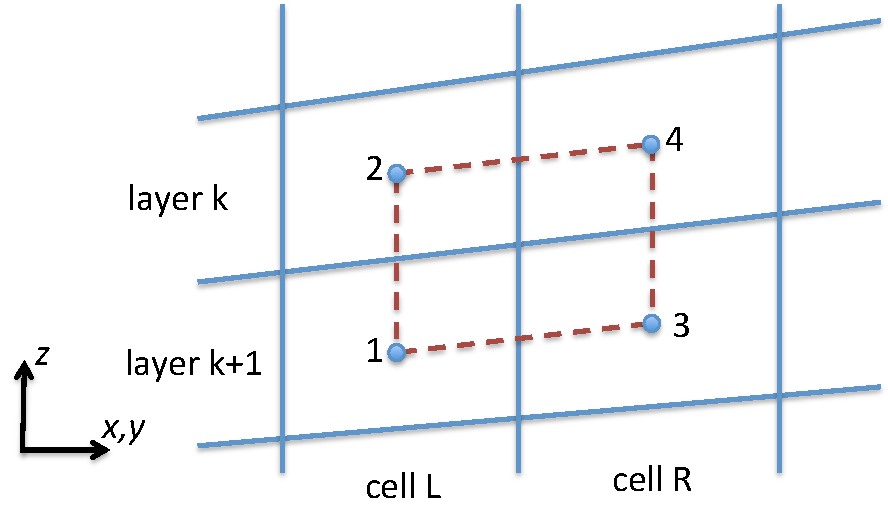
\includegraphics[width=3.5in]{ocean/figures/common_level.pdf}
\caption{Vertical cross-section of ocean grid cells, showing index locations for common level method.  The dots are placed at cell centers in the horizontal and layer mid-depth in the vertical.}
\label{oceanFigure:common level}
\end{figure}

{\bf \large config\_pressure\_gradient\_type = 'Jacobian\_from\_density'}\\
In this formulation the pressure gradient is rewritten in terms of a sea surface height gradient and the vertical integral of a Jacobian,
\begin{eqnarray}
\label{ocean:grad p Jacobian}
- \frac{1}{\rho_0}\nabla_z p &=& - \frac{\rho_s g}{\rho_0}\nabla_s \zeta - \frac{g}{\rho_0}\int_z^\zeta {\mathcal J}(\rho,z)ds, \\
{\mathcal J}(\rho,z) &=& \left. \frac{\partial \rho}{\partial x} \right|_s \frac{\partial z}{\partial s} 
 - \frac{\partial \rho}{\partial s}  \left. \frac{\partial z}{\partial x} \right|_s 
\end{eqnarray}
where $x$ is a general horizontal direction between two cell centers and $s$ is the vertical coordinate reference, i.e.\ $s$ is constant within a layer.  There are many methods to discretize the Jacobian term.  In the common level method, the density is linearly interpolated or extrapolated within each vertical column to a common level $z_\gamma$ (see Figure \ref{oceanFigure:common level}):
\begin{eqnarray}
- \int_z^\zeta {\mathcal J}(\rho,z)ds &=& \overline{\Delta z} \left( \rho^L - \rho^R \right) \\
\overline{\Delta z} &=& \frac{1}{2} \left(z_2-z_1 + z_4-z_3\right) \\
\rho^L &=& \frac{\rho_1\left(z_2-z_\gamma\right) + \rho_2\left(z_\gamma-z_1\right) }{z_2-z_1}\\
\rho^R &=& \frac{\rho_3\left(z_4-z_\gamma\right) + \rho_4\left(z_\gamma-z_3\right) }{z_4-z_3}\\
z_\gamma &=& \left(1-\gamma\right)z_* + \gamma z_c \\
z_* &=&  \frac{z_4 z_2-z_3z_1}{z_4-z_3 + z_2-z_1} \\
z_c &=&  \frac{z_1+z_2+z_3+z_4}{4} 
\end{eqnarray}
where $z_c$ is the depth for the weighted Jacobian method by \citet{Song98mwr}, and $z_*$ is the depth for the standard Jacobian method, which is the depth of intersection of the diagonals of the trapezoidal element in Figure \ref{oceanFigure:common level}.  Here $\gamma$ weights the choice between these two methods for computing the common level $z_\gamma$.  This formulation for the pressure gradient is described in detail in \citet{Shchepetkin_McWilliams03jgr}, Section 2, method 2, and Section 4.  They found that a coefficient of $\gamma=0.5$, which gives equal weights to the standard and weighted Jacobian methods, minimizes the errors in a seamount test problem.

{\bf \large config\_pressure\_gradient\_type = 'Jacobian\_from\_TS'}\\
This formulation is the same as the previous, except that the Jacobian is computed using a linear expansion in potential temperature and salinity.  This option must be used when layers are extremely tilted, such as with sigma coordinates or under an ice shelf, in combination with a nonlinear equation of state.
\begin{eqnarray}
 {\mathcal J}(\rho,z) &=& -\alpha  {\mathcal J}(\theta,z) + \beta  {\mathcal J}(S,z), 
\end{eqnarray}
where
\begin{eqnarray}
\alpha\left( \theta, S, p\right) &=&  -\left. \frac{\partial \rho}{\partial \theta} \right|_{S,p} \\
\beta\left( \theta, S, p\right) &=&  \left. \frac{\partial \rho}{\partial S} \right|_{\theta,p} 
\end{eqnarray}
are the thermal expansion and saline contraction coefficients, computed at a particular  $\left(\theta, S, p\right)$ by the equation of state \citep[eqn 7.16]{Shchepetkin_McWilliams03jgr}.

{\bf \large config\_pressure\_gradient\_type = 'MontgomeryPotential'}\\
For isopycnal vertical coordinates, the user may choose to use the Montgomery potential,
\begin{equation}
\label{ocean:Montgomery Potential}
M = \frac{1}{\rho}p+gz
\end{equation}
and replace the pressure terms above with
\begin{equation}
- \nabla_s M.
\end{equation}
See \citet[section 2.1]{Higdon05jcp} for details on the derivation and computation of the Montgomery potential.

% {\bf \large config\_pressure\_gradient\_type = 'MontgomeryPotential\_and\_density'}
% Same as previous, but this formulation includes an extra term,
% \begin{equation}
% - \nabla_s M + p \nabla_s\left(\frac{1}{\rho} \right),
% \end{equation}
% as described by \citet{Bleck02om}, eqn 1 and end of Appendix A.  This formulation has not been extensively tested and is not supported at this time.

\vspace{0.5in}
{\small
\begin{center}
\begin{longtable}{| p{2.0in} || p{4.0in} |}
	\hline
	{\bf Name} & {\bf Description} \endfirsthead
	\hline 
	{\bf Name} & {\bf Description} (Continued) \endhead
	\hline
	\hline
	\hyperref[sec:nm_sec_config_pressure_gradient_type]{config\_pressure\_gradient\_type} & Form of pressure gradient terms in momentum equation. For most applications, the gradient of pressure and layer mid-depth are appropriate.  For isopycnal coordinates, one may use the gradient of the Montgomery potential. \\
	\hline
	\hyperref[sec:nm_sec_config_density0]{config\_density0} &  Density used as a coefficient of the pressure gradient terms,  $\rho_0$ . This is a constant due to the Boussinesq approximation. \\
	\hline
	\hyperref[sec:nm_sec_config_common_level_weight]{config\_common\_level\_weight} &  The weight between standard Jacobian and weighted Jacobian,  $\gamma$ . \\
	\hline
\end{longtable}
\end{center}
}
\subsection[eos]{eos}
\label{subsec:forward_nm_tab_eos}
Two forms of EOS are supported. The full EOS from \cite{Jackett_McDougall95jaot} and a linear EOS.

\vspace{0.5in}
{\small
\begin{center}
\begin{longtable}{| p{2.0in} || p{4.0in} |}
	\hline
	{\bf Name} & {\bf Description} \endfirsthead
	\hline 
	{\bf Name} & {\bf Description} (Continued) \endhead
	\hline
	\hline
	\hyperref[sec:nm_sec_config_eos_type]{config\_eos\_type} & Character string to choose EOS formulation \\
	\hline
\end{longtable}
\end{center}
}
\subsection[eos\_linear]{eos\_linear}
\label{subsec:forward_nm_tab_eos_linear}
The linear equation of state (leos) is specified as follows:
\begin{equation}
\rho = \rho_{ref} - \alpha_{leos}(T-T_{ref})+\beta_{leos}(S-S_{ref})
\end{equation}
\vspace{0.5in}
{\small
\begin{center}
\begin{longtable}{| p{2.0in} || p{4.0in} |}
	\hline
	{\bf Name} & {\bf Description} \endfirsthead
	\hline 
	{\bf Name} & {\bf Description} (Continued) \endhead
	\hline
	\hline
	\hyperref[sec:nm_sec_config_eos_linear_alpha]{config\_eos\_linear\_alpha} & Linear thermal expansion coefficient \\
	\hline
	\hyperref[sec:nm_sec_config_eos_linear_beta]{config\_eos\_linear\_beta} & Linear haline contraction coefficient \\
	\hline
	\hyperref[sec:nm_sec_config_eos_linear_Tref]{config\_eos\_linear\_Tref} & Reference temperature \\
	\hline
	\hyperref[sec:nm_sec_config_eos_linear_Sref]{config\_eos\_linear\_Sref} & Reference salinity \\
	\hline
	\hyperref[sec:nm_sec_config_eos_linear_densityref]{config\_eos\_linear\_densityref} & Reference density, i.e. density when T=Tref and S=Sref \\
	\hline
\end{longtable}
\end{center}
}
\subsection[split\_explicit\_ts]{split\_explicit\_ts}
\label{subsec:forward_nm_tab_split_explicit_ts}
The split explicit time-stepping method solves the barotropic (vertically-integrated) velocities separately from the remaining baroclinic velocities.  The time step for the barotropic solve is limited by fast surface gravity waves, and so is subcycled within a large timestep of the baroclinic velocity solve.  This provides a 10 to 12-times speed-up over fourth-order Runge-Kutta time stepping.

A single large timestep in the split explicit algorithm may be summarized as
\begin{itemize}
\item Stage 1: solve for baroclinic velocity (3D)
\item Stage 2: solve for barotropic velocity (2D) with explicit sub-cycling
\item Stage 3: update thickness, tracers, density and pressure
\end{itemize}
The algorithm includes iterations within stage 1, within each subcycle of stage 2, and over the full three-stage process.  Further details are provided in \citet[Appendix A.5]{Ringler_ea13om}

\vspace{0.5in}
{\small
\begin{center}
\begin{longtable}{| p{2.0in} || p{4.0in} |}
	\hline
	{\bf Name} & {\bf Description} \endfirsthead
	\hline 
	{\bf Name} & {\bf Description} (Continued) \endhead
	\hline
	\hline
	\hyperref[sec:nm_sec_config_n_ts_iter]{config\_n\_ts\_iter} & number of large iterations over stages 1-3 \\
	\hline
	\hyperref[sec:nm_sec_config_n_bcl_iter_beg]{config\_n\_bcl\_iter\_beg} & number of iterations of stage 1 (baroclinic solve) on the first split-explicit iteration \\
	\hline
	\hyperref[sec:nm_sec_config_n_bcl_iter_mid]{config\_n\_bcl\_iter\_mid} & number of iterations of stage 1 (baroclinic solve) on any split-explicit iterations between first and last \\
	\hline
	\hyperref[sec:nm_sec_config_n_bcl_iter_end]{config\_n\_bcl\_iter\_end} & number of iterations of stage 1 (baroclinic solve) on the last split-explicit iteration \\
	\hline
	\hyperref[sec:nm_sec_config_n_btr_subcycles]{config\_n\_btr\_subcycles} & number of barotropic subcycles in stage 2 \\
	\hline
	\hyperref[sec:nm_sec_config_n_btr_cor_iter]{config\_n\_btr\_cor\_iter} & number of iterations of the velocity corrector step in stage 2 \\
	\hline
	\hyperref[sec:nm_sec_config_vel_correction]{config\_vel\_correction} & If true, the velocity correction term is included in the horizontal advection of thickness and tracers \\
	\hline
	\hyperref[sec:nm_sec_config_btr_subcycle_loop_factor]{config\_btr\_subcycle\_loop\_facto-}\hyperref[sec:nm_sec_config_btr_subcycle_loop_factor]{r}&  Barotropic subcycles proceed from  $t$  to  $t+n\Delta t$ , where  $n$  is this configuration option. \\
	\hline
	\hyperref[sec:nm_sec_config_btr_gam1_velWt1]{config\_btr\_gam1\_velWt1} & Weighting of velocity in the SSH predictor step in stage 2. When zero, previous subcycle time is used; when one, new subcycle time is used. \\
	\hline
	\hyperref[sec:nm_sec_config_btr_gam2_SSHWt1]{config\_btr\_gam2\_SSHWt1} & Weighting of SSH in the velocity corrector step in stage 2. When zero, previous subcycle time is used; when one, new subcycle time is used. \\
	\hline
	\hyperref[sec:nm_sec_config_btr_gam3_velWt2]{config\_btr\_gam3\_velWt2} & Weighting of velocity in the SSH corrector step in stage 2. When zero, previous subcycle time is used; when one, new subcycle time is used. \\
	\hline
	\hyperref[sec:nm_sec_config_btr_solve_SSH2]{config\_btr\_solve\_SSH2} & If true, execute the SSH corrector step in stage 2 \\
	\hline
\end{longtable}
\end{center}
}
\subsection[testing]{testing}
\label{subsec:forward_nm_tab_testing}
\section{Testing}
\label{sec:testing}

\vspace{0.5in}
{\small
\begin{center}
\begin{longtable}{| p{2.0in} || p{4.0in} |}
	\hline
	{\bf Name} & {\bf Description} \endfirsthead
	\hline 
	{\bf Name} & {\bf Description} (Continued) \endhead
	\hline
	\hline
	\hyperref[sec:nm_sec_config_conduct_tests]{config\_conduct\_tests} & If true, run testing suite. This is the overarching control on the test suite. Individual flags must be set to true below to conduct each test. \\
	\hline
	\hyperref[sec:nm_sec_config_test_tensors]{config\_test\_tensors} & If true, tensor operations are tested upon start-up. \\
	\hline
	\hyperref[sec:nm_sec_config_tensor_test_function]{config\_tensor\_test\_function} & Character string to choose tensor test fuction \\
	\hline
\end{longtable}
\end{center}
}
\subsection[debug]{debug}
\label{subsec:forward_nm_tab_debug}
At run-time a user can enable debugging features within MPAS-Ocean. These
features include disabling any tendencies to help determine why an issue might
be happening. Debugging options also include various checks on certain fields,
and the ability to prescribe both a thickness and velocity field at run-time
which are constant throughout a simulation. All options that control these
debugging features are specified within the debug namelist record.

\vspace{0.5in}
{\small
\begin{center}
\begin{longtable}{| p{2.0in} || p{4.0in} |}
	\hline
	{\bf Name} & {\bf Description} \endfirsthead
	\hline 
	{\bf Name} & {\bf Description} (Continued) \endhead
	\hline
	\hline
	\hyperref[sec:nm_sec_config_disable_redi_k33]{config\_disable\_redi\_k33} & If true, disables k33 portion of Redi neutral surface mixing. \\
	\hline
	\hyperref[sec:nm_sec_config_disable_redi_horizontal_term1]{config\_disable\_redi\_horizontal\_t-}\hyperref[sec:nm_sec_config_disable_redi_horizontal_term1]{erm1}& If true, disables first term in horizonal mixing of Redi neutral surface mixing. \\
	\hline
	\hyperref[sec:nm_sec_config_disable_redi_horizontal_term2]{config\_disable\_redi\_horizontal\_t-}\hyperref[sec:nm_sec_config_disable_redi_horizontal_term2]{erm2}& If true, disables first term in horizonal mixing of Redi neutral surface mixing. \\
	\hline
	\hyperref[sec:nm_sec_config_disable_redi_horizontal_term3]{config\_disable\_redi\_horizontal\_t-}\hyperref[sec:nm_sec_config_disable_redi_horizontal_term3]{erm3}& If true, disables first term in horizonal mixing of Redi neutral surface mixing. \\
	\hline
	\hyperref[sec:nm_sec_config_check_zlevel_consistency]{config\_check\_zlevel\_consistency} & Enables a run-time check for consistency for a zlevel grid. Ensures relevant variables correctly define the bottom of the ocean. \\
	\hline
	\hyperref[sec:nm_sec_config_filter_btr_mode]{config\_filter\_btr\_mode} & Enables filtering of the barotropic mode. \\
	\hline
	\hyperref[sec:nm_sec_config_prescribe_velocity]{config\_prescribe\_velocity} & Enables a prescribed velocity field. This velocity field is read on input, and remains constant through a simulation. \\
	\hline
	\hyperref[sec:nm_sec_config_prescribe_thickness]{config\_prescribe\_thickness} & Enables a prescribed thickness field. This thickness field is read on input, and remains constant through a simulation. \\
	\hline
	\hyperref[sec:nm_sec_config_include_KE_vertex]{config\_include\_KE\_vertex} & If true, the kinetic energy in each cell is computed by blending cell-based and vertex-based values of kinetic energy. \\
	\hline
	\hyperref[sec:nm_sec_config_check_tracer_monotonicity]{config\_check\_tracer\_monotonici-}\hyperref[sec:nm_sec_config_check_tracer_monotonicity]{ty}& Enables a change on tracer monotonicity at the end of the monotonic advection routine. Only used if config\_monotonic is set to .true. \\
	\hline
	\hyperref[sec:nm_sec_config_disable_thick_all_tend]{config\_disable\_thick\_all\_tend} & Disables all tendencies on the thickness field. \\
	\hline
	\hyperref[sec:nm_sec_config_disable_thick_hadv]{config\_disable\_thick\_hadv} & Disable tendencies on the thickness field from horizontal advection. \\
	\hline
	\hyperref[sec:nm_sec_config_disable_thick_vadv]{config\_disable\_thick\_vadv} & Disables tendencies on the thickness field from vertical advection. \\
	\hline
	\hyperref[sec:nm_sec_config_disable_thick_sflux]{config\_disable\_thick\_sflux} & Disables tendencies on the thickness field from surface fluxes. \\
	\hline
	\hyperref[sec:nm_sec_config_disable_vel_all_tend]{config\_disable\_vel\_all\_tend} & Disables all tendencies on the velocity field. \\
	\hline
	\hyperref[sec:nm_sec_config_disable_vel_coriolis]{config\_disable\_vel\_coriolis} & Diables tendencies on the velocity field from the Coriolis force. \\
	\hline
	\hyperref[sec:nm_sec_config_disable_vel_pgrad]{config\_disable\_vel\_pgrad} & Disables tendencies on the velocity field from the horizontal pressure gradient. \\
	\hline
	\hyperref[sec:nm_sec_config_disable_vel_hmix]{config\_disable\_vel\_hmix} & Disables tendencies on the velocity field from horizontal mixing. \\
	\hline
	\hyperref[sec:nm_sec_config_disable_vel_windstress]{config\_disable\_vel\_windstress} & Disables tendencies on the velocity field from horizontal wind stress. \\
	\hline
	\hyperref[sec:nm_sec_config_disable_vel_vmix]{config\_disable\_vel\_vmix} & Disables tendencies on the velocity field from vertical mixing. \\
	\hline
	\hyperref[sec:nm_sec_config_disable_vel_vadv]{config\_disable\_vel\_vadv} & Disables tendencies on the velocity field from vertical advection. \\
	\hline
	\hyperref[sec:nm_sec_config_disable_tr_all_tend]{config\_disable\_tr\_all\_tend} & Disables all tendencies on tracer fields. \\
	\hline
	\hyperref[sec:nm_sec_config_disable_tr_adv]{config\_disable\_tr\_adv} & Disables tendencies on tracer fields from advection, both horizontal and vertical. \\
	\hline
	\hyperref[sec:nm_sec_config_disable_tr_hmix]{config\_disable\_tr\_hmix} & Disables tendencies on tracer fields from horizontal mixing. \\
	\hline
	\hyperref[sec:nm_sec_config_disable_tr_vmix]{config\_disable\_tr\_vmix} & Disables tendencies on tracer fields from vertical mixing. \\
	\hline
	\hyperref[sec:nm_sec_config_disable_tr_sflux]{config\_disable\_tr\_sflux} & Disables tendencies on tracer fields from surface fluxes. \\
	\hline
	\hyperref[sec:nm_sec_config_disable_tr_nonlocalflux]{config\_disable\_tr\_nonlocalflux} & Disables tendencies on the tracer fields from CVMix/KPP nonlocal fluxes. \\
	\hline
\end{longtable}
\end{center}
}
\subsection[global\_stats]{global\_stats}
\label{subsec:forward_nm_tab_global_stats}
\vspace{0.5in}
{\small
\begin{center}
\begin{longtable}{| p{2.0in} || p{4.0in} |}
	\hline
	{\bf Name} & {\bf Description} \endfirsthead
	\hline 
	{\bf Name} & {\bf Description} (Continued) \endhead
	\hline
	\hline
	\hyperref[sec:nm_sec_config_use_global_stats]{config\_use\_global\_stats} & If true, ocean analysis member global\_stats is called. \\
	\hline
	\hyperref[sec:nm_sec_config_global_stats_compute_interval]{config\_global\_stats\_compute\_int-}\hyperref[sec:nm_sec_config_global_stats_compute_interval]{erval}& Timestamp determining how often analysis member computation should be performed. \\
	\hline
	\hyperref[sec:nm_sec_config_global_stats_compute_startup]{config\_global\_stats\_compute\_st-}\hyperref[sec:nm_sec_config_global_stats_compute_startup]{artup}& Logical flag determining if an analysis member computation occurs on start-up. \\
	\hline
\end{longtable}
\end{center}
}
\subsection[zonal\_mean]{zonal\_mean}
\label{subsec:forward_nm_tab_zonal_mean}
\vspace{0.5in}
{\small
\begin{center}
\begin{longtable}{| p{2.0in} || p{4.0in} |}
	\hline
	{\bf Name} & {\bf Description} \endfirsthead
	\hline 
	{\bf Name} & {\bf Description} (Continued) \endhead
	\hline
	\hline
	\hyperref[sec:nm_sec_config_use_zonal_mean]{config\_use\_zonal\_mean} & If true, ocean analysis member zonal\_mean is called. \\
	\hline
	\hyperref[sec:nm_sec_config_zonal_mean_compute_interval]{config\_zonal\_mean\_compute\_inte-}\hyperref[sec:nm_sec_config_zonal_mean_compute_interval]{rval}& Timestamp determining how often analysis member computation should be performed. \\
	\hline
	\hyperref[sec:nm_sec_config_zonal_mean_compute_startup]{config\_zonal\_mean\_compute\_sta-}\hyperref[sec:nm_sec_config_zonal_mean_compute_startup]{rtup}& Logical flag determining if an analysis member computation occurs on start-up. \\
	\hline
	\hyperref[sec:nm_sec_config_number_zonal_mean_bins]{config\_number\_zonal\_mean\_bins} & Number of bins used for zonal mean.  Must be less than or equal to the dimension nZonalMeanBins (set in Registry). \\
	\hline
	\hyperref[sec:nm_sec_config_min_zonal_mean_bin]{config\_min\_zonal\_mean\_bin} & minimum bin boundary value.  If set to -1.0e34, the minimum value in the domain is found. \\
	\hline
	\hyperref[sec:nm_sec_config_max_zonal_mean_bin]{config\_max\_zonal\_mean\_bin} & maximum bin boundary value.  If set to -1.0e34, the maximum value in the domain is found. \\
	\hline
\end{longtable}
\end{center}
}
\section[Variable definitions]{\hyperref[chap:variable_sections]{Variable definitions}}
\label{sec:forward_variable_tables}
Embedded links point to more detailed variable information in the appendix.
\subsection[state]{\hyperref[sec:var_sec_state]{state}}
\label{subsec:forward_var_tab_state}
The state data structure contains a set of prognostic and diagnostic fields
that are time dependent. The fields contained inside of state have two time
levels available in the default version of MPAS-Ocean.

\vspace{0.5in}
{\small
\begin{center}
\begin{longtable}{| p{2.0in} | p{4.0in} |}
	\hline
	{\bf Name} & {\bf Description} \endfirsthead
	\hline 
	{\bf Name} & {\bf Description} (Continued) \endhead
	\hline
	\hyperref[subsec:var_sec_state_temperature]{temperature} & potential temperature \\
	\hline
	\hyperref[subsec:var_sec_state_salinity]{salinity} & salinity \\
	\hline
	\hyperref[subsec:var_sec_state_tracer1]{tracer1} & tracer \\
	\hline
	\hyperref[subsec:var_sec_state_normalVelocity]{normalVelocity} & horizonal velocity, normal component to an edge \\
	\hline
	\hyperref[subsec:var_sec_state_layerThickness]{layerThickness} & layer thickness \\
	\hline
	\hyperref[subsec:var_sec_state_ssh]{ssh} & sea surface height \\
	\hline
	\hyperref[subsec:var_sec_state_highFreqThickness]{highFreqThickness} & high frequency-filtered layer thickness \\
	\hline
	\hyperref[subsec:var_sec_state_lowFreqDivergence]{lowFreqDivergence} & low frequency-filtered divergence \\
	\hline
	\hyperref[subsec:var_sec_state_normalBarotropicVelocity]{normalBarotropicVelocity} & barotropic velocity, used in split-explicit time-stepping \\
	\hline
	\hyperref[subsec:var_sec_state_normalBarotropicVelocitySubcycle]{normalBarotropicVelocitySubcy-}\hyperref[subsec:var_sec_state_normalBarotropicVelocitySubcycle]{cle  }& barotropic velocity, used in subcycling in stage 2 of split-explicit time-stepping \\
	\hline
	\hyperref[subsec:var_sec_state_sshSubcycle]{sshSubcycle} & sea surface height, used in subcycling in stage 2 of split-explicit time-stepping \\
	\hline
	\hyperref[subsec:var_sec_state_normalBaroclinicVelocity]{normalBaroclinicVelocity} & baroclinic velocity, used in split-explicit time-stepping \\
	\hline
\end{longtable}
\end{center}
}
\subsection[mesh]{\hyperref[sec:var_sec_mesh]{mesh}}
\label{subsec:forward_var_tab_mesh}
The mesh data type contains a single time level. The fields inside the mesh
structure are not assumed to be time dependent. This data structure contains
fields that describe the mesh, and the connectivity of the mesh. Several of the
fields contained in this structure are shared throughout all MPAS dynamical
cores.

\vspace{0.5in}
{\small
\begin{center}
\begin{longtable}{| p{2.0in} | p{4.0in} |}
	\hline
	{\bf Name} & {\bf Description} \endfirsthead
	\hline 
	{\bf Name} & {\bf Description} (Continued) \endhead
	\hline
	\hyperref[subsec:var_sec_mesh_latCell]{latCell} & Latitude location of cell centers in radians. \\
	\hline
	\hyperref[subsec:var_sec_mesh_lonCell]{lonCell} & Longitude location of cell centers in radians. \\
	\hline
	\hyperref[subsec:var_sec_mesh_xCell]{xCell} & X Coordinate in cartesian space of cell centers. \\
	\hline
	\hyperref[subsec:var_sec_mesh_yCell]{yCell} & Y Coordinate in cartesian space of cell centers. \\
	\hline
	\hyperref[subsec:var_sec_mesh_zCell]{zCell} & Z Coordinate in cartesian space of cell centers. \\
	\hline
	\hyperref[subsec:var_sec_mesh_indexToCellID]{indexToCellID} & List of global cell IDs. \\
	\hline
	\hyperref[subsec:var_sec_mesh_latEdge]{latEdge} & Latitude location of edge midpoints in radians. \\
	\hline
	\hyperref[subsec:var_sec_mesh_lonEdge]{lonEdge} & Longitude location of edge midpoints in radians. \\
	\hline
	\hyperref[subsec:var_sec_mesh_xEdge]{xEdge} & X Coordinate in cartesian space of edge midpoints. \\
	\hline
	\hyperref[subsec:var_sec_mesh_yEdge]{yEdge} & Y Coordinate in cartesian space of edge midpoints. \\
	\hline
	\hyperref[subsec:var_sec_mesh_zEdge]{zEdge} & Z Coordinate in cartesian space of edge midpoints. \\
	\hline
	\hyperref[subsec:var_sec_mesh_indexToEdgeID]{indexToEdgeID} & List of global edge IDs. \\
	\hline
	\hyperref[subsec:var_sec_mesh_latVertex]{latVertex} & Latitude location of vertices in radians. \\
	\hline
	\hyperref[subsec:var_sec_mesh_lonVertex]{lonVertex} & Longitude location of vertices in radians. \\
	\hline
	\hyperref[subsec:var_sec_mesh_xVertex]{xVertex} & X Coordinate in cartesian space of vertices. \\
	\hline
	\hyperref[subsec:var_sec_mesh_yVertex]{yVertex} & Y Coordinate in cartesian space of vertices. \\
	\hline
	\hyperref[subsec:var_sec_mesh_zVertex]{zVertex} & Z Coordinate in cartesian space of vertices. \\
	\hline
	\hyperref[subsec:var_sec_mesh_indexToVertexID]{indexToVertexID} & List of global vertex IDs. \\
	\hline
	\hyperref[subsec:var_sec_mesh_meshDensity]{meshDensity} & Value of density function used to generate a particular mesh at cell centers. \\
	\hline
	\hyperref[subsec:var_sec_mesh_meshScalingDel2]{meshScalingDel2} & Coefficient to Laplacian mixing terms in momentum and tracer equations, so that viscosity and diffusion scale with mesh. \\
	\hline
	\hyperref[subsec:var_sec_mesh_meshScalingDel4]{meshScalingDel4} & Coefficient to biharmonic mixing terms in momentum and tracer equations, so that biharmonic viscosity and diffusion coefficients scale with mesh. \\
	\hline
	\hyperref[subsec:var_sec_mesh_meshScaling]{meshScaling} & Coefficient used for mesh scaling, such as the Leith parameter. \\
	\hline
	\hyperref[subsec:var_sec_mesh_cellsOnEdge]{cellsOnEdge} & List of cells that straddle each edge. \\
	\hline
	\hyperref[subsec:var_sec_mesh_nEdgesOnCell]{nEdgesOnCell} & Number of edges that border each cell. \\
	\hline
	\hyperref[subsec:var_sec_mesh_nEdgesOnEdge]{nEdgesOnEdge} & Number of edges that surround each of the cells that straddle each edge. These edges are used to reconstruct the tangential velocities. \\
	\hline
	\hyperref[subsec:var_sec_mesh_edgesOnCell]{edgesOnCell} & List of edges that border each cell. \\
	\hline
	\hyperref[subsec:var_sec_mesh_edgesOnEdge]{edgesOnEdge} & List of edges that border each of the cells that straddle each edge. \\
	\hline
	\hyperref[subsec:var_sec_mesh_weightsOnEdge]{weightsOnEdge} & Reconstruction weights associated with each of the edgesOnEdge. \\
	\hline
	\hyperref[subsec:var_sec_mesh_dvEdge]{dvEdge} & Length of each edge, computed as the distance between verticesOnEdge. \\
	\hline
	\hyperref[subsec:var_sec_mesh_dcEdge]{dcEdge} & Length of each edge, computed as the distance between cellsOnEdge. \\
	\hline
	\hyperref[subsec:var_sec_mesh_angleEdge]{angleEdge} & Angle the edge normal makes with local eastward direction. \\
	\hline
	\hyperref[subsec:var_sec_mesh_areaCell]{areaCell} & Area of each cell in the primary grid. \\
	\hline
	\hyperref[subsec:var_sec_mesh_areaTriangle]{areaTriangle} & Area of each cell (triangle) in the dual grid. \\
	\hline
	\hyperref[subsec:var_sec_mesh_edgeNormalVectors]{edgeNormalVectors} & Normal unit vector defined at an edge. \\
	\hline
	\hyperref[subsec:var_sec_mesh_edgeTangentVectors]{edgeTangentVectors} & Tangent unit vector defined at an edge. \\
	\hline
	\hyperref[subsec:var_sec_mesh_localVerticalUnitVectors]{localVerticalUnitVectors} & Unit surface normal vectors defined at cell centers. \\
	\hline
	\hyperref[subsec:var_sec_mesh_cellTangentPlane]{cellTangentPlane} & The two vectors that define a tangent plane at a cell center. \\
	\hline
	\hyperref[subsec:var_sec_mesh_cellsOnCell]{cellsOnCell} & List of cells that neighbor each cell. \\
	\hline
	\hyperref[subsec:var_sec_mesh_verticesOnCell]{verticesOnCell} & List of vertices that border each cell. \\
	\hline
	\hyperref[subsec:var_sec_mesh_verticesOnEdge]{verticesOnEdge} & List of vertices that straddle each edge. \\
	\hline
	\hyperref[subsec:var_sec_mesh_edgesOnVertex]{edgesOnVertex} & List of edges that share a vertex as an endpoint. \\
	\hline
	\hyperref[subsec:var_sec_mesh_cellsOnVertex]{cellsOnVertex} & List of cells that share a vertex. \\
	\hline
	\hyperref[subsec:var_sec_mesh_kiteAreasOnVertex]{kiteAreasOnVertex} & Area of the portions of each dual cell that are part of each cellsOnVertex. \\
	\hline
	\hyperref[subsec:var_sec_mesh_fEdge]{fEdge} & Coriolis parameter at edges. \\
	\hline
	\hyperref[subsec:var_sec_mesh_fVertex]{fVertex} & Coriolis parameter at vertices. \\
	\hline
	\hyperref[subsec:var_sec_mesh_fCell]{fCell} & Coriolis parameter at cell centers. \\
	\hline
	\hyperref[subsec:var_sec_mesh_bottomDepth]{bottomDepth} & Depth of the bottom of the ocean. Given as a positive distance from sea level. \\
	\hline
	\hyperref[subsec:var_sec_mesh_derivTwo]{derivTwo} & Value of the second derivative of the polynomial used for reconstruction of cell center quantities at edges. \\
	\hline
	\hyperref[subsec:var_sec_mesh_advCoefs]{advCoefs} & Weighting coefficients used for reconstruction of cell center quantities at edges. Used in advection routines. \\
	\hline
	\hyperref[subsec:var_sec_mesh_advCoefs3rd]{advCoefs3rd} & Wegihting coefficients used for reconstruction of cell center quantities at edges. Used in advection routines. \\
	\hline
	\hyperref[subsec:var_sec_mesh_advCellsForEdge]{advCellsForEdge} & List of cells used to reconstruct a cell quantity at an edge. Used in advection routines. \\
	\hline
	\hyperref[subsec:var_sec_mesh_nAdvCellsForEdge]{nAdvCellsForEdge} & Number of cells used in reconstruction of cell center quantities at an edge. Used in advection routines. \\
	\hline
	\hyperref[subsec:var_sec_mesh_highOrderAdvectionMask]{highOrderAdvectionMask} & Mask for high order advection. Values are 1 if high order is used, and 0 if not. \\
	\hline
	\hyperref[subsec:var_sec_mesh_coeffs_reconstruct]{coeffs\_reconstruct} & Coefficients to reconstruct velocity vectors at cells centers. \\
	\hline
	\hyperref[subsec:var_sec_mesh_maxLevelCell]{maxLevelCell} & Index to the last active ocean cell in each column. \\
	\hline
	\hyperref[subsec:var_sec_mesh_maxLevelEdgeTop]{maxLevelEdgeTop} & Index to the last edge in a column with active ocean cells on both sides of it. \\
	\hline
	\hyperref[subsec:var_sec_mesh_maxLevelEdgeBot]{maxLevelEdgeBot} & Index to the last edge in a column with at least one active ocean cell on either side of it. \\
	\hline
	\hyperref[subsec:var_sec_mesh_maxLevelVertexTop]{maxLevelVertexTop} & Index to the last vertex in a column with all active cells around it. \\
	\hline
	\hyperref[subsec:var_sec_mesh_maxLevelVertexBot]{maxLevelVertexBot} & Index to the last vertex in a column with at least one active ocean cell around it. \\
	\hline
	\hyperref[subsec:var_sec_mesh_refBottomDepth]{refBottomDepth} & Reference depth of ocean for each vertical level. Used in 'z-level' type runs. \\
	\hline
	\hyperref[subsec:var_sec_mesh_refBottomDepthTopOfCell]{refBottomDepthTopOfCell} & Reference depth of ocean for each vertical interface. Used in 'z-level' type runs. \\
	\hline
	\hyperref[subsec:var_sec_mesh_vertCoordMovementWeights]{vertCoordMovementWeights} & Weights used for distribution of sea surface heigh purturbations through multiple vertical levels. \\
	\hline
	\hyperref[subsec:var_sec_mesh_boundaryEdge]{boundaryEdge} & Mask for determining boundary edges. A boundary edge has only one active ocean cell neighboring it. \\
	\hline
	\hyperref[subsec:var_sec_mesh_boundaryVertex]{boundaryVertex} & Mask for determining boundary vertices. A boundary vertex has at least one inactive cell neighboring it. \\
	\hline
	\hyperref[subsec:var_sec_mesh_boundaryCell]{boundaryCell} & Mask for determining boundary cells. A boundary cell has at least one inactive cell neighboring it. \\
	\hline
	\hyperref[subsec:var_sec_mesh_edgeMask]{edgeMask} & Mask on edges that determines if computations should be done on edge. \\
	\hline
	\hyperref[subsec:var_sec_mesh_vertexMask]{vertexMask} & Mask on vertices that determines if computations should be done on vertice. \\
	\hline
	\hyperref[subsec:var_sec_mesh_cellMask]{cellMask} & Mask on cells that determines if computations should be done on cell. \\
	\hline
	\hyperref[subsec:var_sec_mesh_temperatureRestore]{temperatureRestore} & Temperature restoring field, for restoring temperature at the surface. \\
	\hline
	\hyperref[subsec:var_sec_mesh_salinityRestore]{salinityRestore} & Salinity restoring field, for restoring salinity at the surface. \\
	\hline
	\hyperref[subsec:var_sec_mesh_edgeSignOnCell]{edgeSignOnCell} & Sign of edge contributions to a cell for each edge on cell. Used for bit-reproducible loops. Represents directionality of vector connecting cells. \\
	\hline
	\hyperref[subsec:var_sec_mesh_edgeSignOnVertex]{edgeSignOnVertex} & Sign of edge contributions to a vertex for each edge on vertex. Used for bit-reproducible loops. Represents directionality of vector connecting vertices. \\
	\hline
	\hyperref[subsec:var_sec_mesh_kiteIndexOnCell]{kiteIndexOnCell} & Index of kite in dual grid, based on verticesOnCell. \\
	\hline
\end{longtable}
\end{center}
}
\subsection[verticalMesh]{\hyperref[sec:var_sec_verticalMesh]{verticalMesh}}
\label{subsec:forward_var_tab_verticalMesh}
The vertical mesh data type contains a single time level. The fields inside the
vertical mesh structure are not assumed to be time dependent. This data
structure contains fields that describe the vertical mesh and are used for
various types of vertical meshes.

\vspace{0.5in}
{\small
\begin{center}
\begin{longtable}{| p{2.0in} | p{4.0in} |}
	\hline
	{\bf Name} & {\bf Description} \endfirsthead
	\hline 
	{\bf Name} & {\bf Description} (Continued) \endhead
	\hline
	\hyperref[subsec:var_sec_verticalMesh_restingThickness]{restingThickness} & Layer thickness when the ocean is at rest, i.e. without SSH or internal perturbations. \\
	\hline
	\hyperref[subsec:var_sec_verticalMesh_refZMid]{refZMid} & Reference mid z-coordinate of ocean for each vertical level. This has a negative value. \\
	\hline
	\hyperref[subsec:var_sec_verticalMesh_refLayerThickness]{refLayerThickness} & Reference layerThickness of ocean for each vertical level. \\
	\hline
\end{longtable}
\end{center}
}
\subsection[tend]{\hyperref[sec:var_sec_tend]{tend}}
\label{subsec:forward_var_tab_tend}
The tend data structure represents the tendencies used to time step the
prognostic variables within the state structure. 

\vspace{0.5in}
{\small
\begin{center}
\begin{longtable}{| p{2.0in} | p{4.0in} |}
	\hline
	{\bf Name} & {\bf Description} \endfirsthead
	\hline 
	{\bf Name} & {\bf Description} (Continued) \endhead
	\hline
	\hyperref[subsec:var_sec_tend_tendTemperature]{tendTemperature} & time tendency of potential temperature \\
	\hline
	\hyperref[subsec:var_sec_tend_tendSalinity]{tendSalinity} & time tendency of salinity measured as change in practical salinity units per second \\
	\hline
	\hyperref[subsec:var_sec_tend_tendTracer1]{tendTracer1} & test tracer \\
	\hline
	\hyperref[subsec:var_sec_tend_tendNormalVelocity]{tendNormalVelocity} & time tendency of normal component of velocity \\
	\hline
	\hyperref[subsec:var_sec_tend_tendLayerThickness]{tendLayerThickness} & time tendency of layer thickness \\
	\hline
	\hyperref[subsec:var_sec_tend_tendSSH]{tendSSH} & time tendency of sea-surface height \\
	\hline
	\hyperref[subsec:var_sec_tend_tendHighFreqThickness]{tendHighFreqThickness} & time tendency of high frequency-filtered layer thickness \\
	\hline
	\hyperref[subsec:var_sec_tend_tendLowFreqDivergence]{tendLowFreqDivergence} & time tendency of low frequency-filtered divergence \\
	\hline
\end{longtable}
\end{center}
}
\subsection[diagnostics]{\hyperref[sec:var_sec_diagnostics]{diagnostics}}
\label{subsec:forward_var_tab_diagnostics}
The diagnostics type contains a set of diagnostics variables that are only
generally used in specific parts of MPAS-Ocean.

\vspace{0.5in}
{\small
\begin{center}
\begin{longtable}{| p{2.0in} | p{4.0in} |}
	\hline
	{\bf Name} & {\bf Description} \endfirsthead
	\hline 
	{\bf Name} & {\bf Description} (Continued) \endhead
	\hline
	\hyperref[subsec:var_sec_diagnostics_xtime]{xtime} & model time, with format 'YYYY-MM-DD\_HH:MM:SS' \\
	\hline
	\hyperref[subsec:var_sec_diagnostics_temperatureSurfaceValue]{temperatureSurfaceValue} & potential temperature extrapolated to ocean surface \\
	\hline
	\hyperref[subsec:var_sec_diagnostics_salinitySurfaceValue]{salinitySurfaceValue} & salinity extrapolated to ocean surface \\
	\hline
	\hyperref[subsec:var_sec_diagnostics_tracer1SurfaceValue]{tracer1SurfaceValue} & Tracer of 1 extrapolated to ocean surface \\
	\hline
	\hyperref[subsec:var_sec_diagnostics_temperatureSurfaceLayerValue]{temperatureSurfaceLayerValu-}\hyperref[subsec:var_sec_diagnostics_temperatureSurfaceLayerValue]{e}  & potential temperature averaged over ocean surface layer (generally 0.1 of the ocean boundary layer) \\
	\hline
	\hyperref[subsec:var_sec_diagnostics_salinitySurfaceLayerValue]{salinitySurfaceLayerValue} & salinity averaged over ocean surface layer (generally 0.1 of the ocean boundary layer) \\
	\hline
	\hyperref[subsec:var_sec_diagnostics_tracer1SurfaceLayerValue]{tracer1SurfaceLayerValue} & Tracer of 1 averaged over ocean surface layer (generally 0.1 of the ocean boundary layer) \\
	\hline
	\hyperref[subsec:var_sec_diagnostics_normalVelocitySurfaceLayer]{normalVelocitySurfaceLayer} & normal velocity averaged over ocean surface layer (generally 0.1 of the ocean boundary layer) \\
	\hline
	\hyperref[subsec:var_sec_diagnostics_surfaceVelocityZonal]{surfaceVelocityZonal} & Zonal surface velocity reconstructed at cell centers \\
	\hline
	\hyperref[subsec:var_sec_diagnostics_surfaceVelocityMeridional]{surfaceVelocityMeridional} & Meridional surface velocity reconstructed at cell centers \\
	\hline
	\hyperref[subsec:var_sec_diagnostics_SSHGradientZonal]{SSHGradientZonal} & Zonal gradient of SSH reconstructed at cell centers \\
	\hline
	\hyperref[subsec:var_sec_diagnostics_SSHGradientMeridional]{SSHGradientMeridional} & Meridional gradient of SSH reconstructed at cell centers \\
	\hline
	\hyperref[subsec:var_sec_diagnostics_zMid]{zMid} & z-coordinate of the mid-depth of the layer \\
	\hline
	\hyperref[subsec:var_sec_diagnostics_zTop]{zTop} & z-coordinate of the top of the layer \\
	\hline
	\hyperref[subsec:var_sec_diagnostics_density]{density} & density \\
	\hline
	\hyperref[subsec:var_sec_diagnostics_displacedDensity]{displacedDensity} & Density displaced adiabatically to the mid-depth one layer deeper.  That is, layer k has been displaced to the depth of layer k+1. \\
	\hline
	\hyperref[subsec:var_sec_diagnostics_potentialDensity]{potentialDensity} & potential density: density displaced adiabatically to the mid-depth of top layer \\
	\hline
	\hyperref[subsec:var_sec_diagnostics_inSituThermalExpansionCoeff]{inSituThermalExpansionCoeff} &  Thermal expansion coefficient (alpha), defined as  $-1/\rho d\rho/dT$  (note negative sign).  This is in situ, i.e. not displaced to another depth. \\
	\hline
	\hyperref[subsec:var_sec_diagnostics_inSituSalineContractionCoeff]{inSituSalineContractionCoeff} &  Saline contraction coefficient (beta), defined as  $1/\rho d\rho/dS$ .  This is also called the haline contraction coefficient.  This is in situ, i.e. not displaced to another depth. \\
	\hline
	\hyperref[subsec:var_sec_diagnostics_BruntVaisalaFreqTop]{BruntVaisalaFreqTop} & Brunt Vaisala frequency defined at the center (horizontally) and top (vertically) of cell \\
	\hline
	\hyperref[subsec:var_sec_diagnostics_montgomeryPotential]{montgomeryPotential} & Montgomery potential, may be used as the pressure for isopycnal coordinates. \\
	\hline
	\hyperref[subsec:var_sec_diagnostics_pressure]{pressure} & pressure used in the momentum equation \\
	\hline
	\hyperref[subsec:var_sec_diagnostics_normalTransportVelocity]{normalTransportVelocity} & horizontal velocity used to transport mass and tracers \\
	\hline
	\hyperref[subsec:var_sec_diagnostics_vertAleTransportTop]{vertAleTransportTop} & vertical transport through the layer interface at the top of the cell \\
	\hline
	\hyperref[subsec:var_sec_diagnostics_vertVelocityTop]{vertVelocityTop} & vertical velocity defined at center (horizonally) and top (vertically) of cell \\
	\hline
	\hyperref[subsec:var_sec_diagnostics_vertTransportVelocityTop]{vertTransportVelocityTop} & vertical tracer-transport velocity defined at center (horizonally) and top (vertically) of cell.  This is not the vertical ALE transport, but is Eulerian (fixed-frame) in the vertical, and computed from the continuity equation from the horizontal total tracer-transport velocity. \\
	\hline
	\hyperref[subsec:var_sec_diagnostics_vertGMBolusVelocityTop]{vertGMBolusVelocityTop} & vertical tracer-transport velocity defined at center (horizonally) and top (vertically) of cell.  This is not the vertical ALE transport, but is Eulerian (fixed-frame) in the vertical, and computed from the continuity equation from the horizontal GM Bolus velocity. \\
	\hline
	\hyperref[subsec:var_sec_diagnostics_tangentialVelocity]{tangentialVelocity} & horizontal velocity, tangential to an edge \\
	\hline
	\hyperref[subsec:var_sec_diagnostics_layerThicknessEdge]{layerThicknessEdge} & layer thickness averaged from cell center to edges \\
	\hline
	\hyperref[subsec:var_sec_diagnostics_layerThicknessVertex]{layerThicknessVertex} & layer thickness averaged from cell center to vertices \\
	\hline
	\hyperref[subsec:var_sec_diagnostics_kineticEnergyCell]{kineticEnergyCell} & kinetic energy of horizonal velocity on cells \\
	\hline
	\hyperref[subsec:var_sec_diagnostics_hEddyFlux]{hEddyFlux} & Eddy flux in Gent-McWilliams eddy parameterization \\
	\hline
	\hyperref[subsec:var_sec_diagnostics_hKappa]{hKappa} & kappa parameter for Gent-McWilliams eddy parameterization \\
	\hline
	\hyperref[subsec:var_sec_diagnostics_hKappaQ]{hKappaQ} & kappaQ parameter for Gent-McWilliams eddy parameterization \\
	\hline
	\hyperref[subsec:var_sec_diagnostics_viscosity]{viscosity} & horizontal viscosity \\
	\hline
	\hyperref[subsec:var_sec_diagnostics_divergence]{divergence} & divergence of horizonal velocity \\
	\hline
	\hyperref[subsec:var_sec_diagnostics_circulation]{circulation} & area-integrated vorticity \\
	\hline
	\hyperref[subsec:var_sec_diagnostics_relativeVorticity]{relativeVorticity} & curl of horizontal velocity, defined at vertices \\
	\hline
	\hyperref[subsec:var_sec_diagnostics_relativeVorticityCell]{relativeVorticityCell} & curl of horizontal velocity, averaged from vertices to cell centers \\
	\hline
	\hyperref[subsec:var_sec_diagnostics_normalizedRelativeVorticityEdge]{normalizedRelativeVorticityEdge} & curl of horizontal velocity divided by layer thickness, averaged from vertices to edges \\
	\hline
	\hyperref[subsec:var_sec_diagnostics_normalizedPlanetaryVorticityEdge]{normalizedPlanetaryVorticityEd-}\hyperref[subsec:var_sec_diagnostics_normalizedPlanetaryVorticityEdge]{ge  }& earth's rotational rate (Coriolis parameter, f) divided by layer thickness, averaged from vertices to edges \\
	\hline
	\hyperref[subsec:var_sec_diagnostics_normalizedRelativeVorticityCell]{normalizedRelativeVorticityCell} & curl of horizontal velocity divided by layer thickness, averaged from vertices to cell centers \\
	\hline
	\hyperref[subsec:var_sec_diagnostics_barotropicForcing]{barotropicForcing} & Barotropic tendency computed from the baroclinic equations in stage 1 of the split-explicit algorithm. \\
	\hline
	\hyperref[subsec:var_sec_diagnostics_barotropicThicknessFlux]{barotropicThicknessFlux} & Barotropic thickness flux at each edge, used to advance sea surface height in each subcycle of stage 2 of the split-explicit algorithm. \\
	\hline
	\hyperref[subsec:var_sec_diagnostics_velocityX]{velocityX} & component of horizontal velocity in the x-direction (cartesian) \\
	\hline
	\hyperref[subsec:var_sec_diagnostics_velocityY]{velocityY} & component of horizontal velocity in the y-direction (cartesian) \\
	\hline
	\hyperref[subsec:var_sec_diagnostics_velocityZ]{velocityZ} & component of horizontal velocity in the z-direction (cartesian) \\
	\hline
	\hyperref[subsec:var_sec_diagnostics_velocityZonal]{velocityZonal} & component of horizontal velocity in the eastward direction \\
	\hline
	\hyperref[subsec:var_sec_diagnostics_velocityMeridional]{velocityMeridional} & component of horizontal velocity in the northward direction \\
	\hline
	\hyperref[subsec:var_sec_diagnostics_transportVelocityX]{transportVelocityX} & component of horizontal velocity used to transport mass and tracers in the x-direction (cartesian) \\
	\hline
	\hyperref[subsec:var_sec_diagnostics_transportVelocityY]{transportVelocityY} & component of horizontal velocity used to transport mass and tracers in the y-direction (cartesian) \\
	\hline
	\hyperref[subsec:var_sec_diagnostics_transportVelocityZ]{transportVelocityZ} & component of horizontal velocity used to transport mass and tracers in the z-direction (cartesian) \\
	\hline
	\hyperref[subsec:var_sec_diagnostics_transportVelocityZonal]{transportVelocityZonal} & component of horizontal velocity used to transport mass and tracers in the eastward direction \\
	\hline
	\hyperref[subsec:var_sec_diagnostics_transportVelocityMeridional]{transportVelocityMeridional} & component of horizontal velocity used to transport mass and tracers in the northward direction \\
	\hline
	\hyperref[subsec:var_sec_diagnostics_gradSSH]{gradSSH} & Gradient of sea surface height at edges. \\
	\hline
	\hyperref[subsec:var_sec_diagnostics_gradSSHX]{gradSSHX} & X Component of the gradient of sea surface height at cell centers. \\
	\hline
	\hyperref[subsec:var_sec_diagnostics_gradSSHY]{gradSSHY} & Y Component of the gradient of sea surface height at cell centers. \\
	\hline
	\hyperref[subsec:var_sec_diagnostics_gradSSHZ]{gradSSHZ} & Z Component of the gradient of sea surface height at cell centers. \\
	\hline
	\hyperref[subsec:var_sec_diagnostics_gradSSHZonal]{gradSSHZonal} & Zonal Component of the gradient of sea surface height at cell centers. \\
	\hline
	\hyperref[subsec:var_sec_diagnostics_gradSSHMeridional]{gradSSHMeridional} & Meridional Component of the gradient of sea surface height at cell centers. \\
	\hline
	\hyperref[subsec:var_sec_diagnostics_normalGMBolusVelocity]{normalGMBolusVelocity} & Bolus velocity in Gent-McWilliams eddy parameterization \\
	\hline
	\hyperref[subsec:var_sec_diagnostics_GMBolusVelocityX]{GMBolusVelocityX} & Bolus velocity in Gent-McWilliams eddy parameterization, x-direction \\
	\hline
	\hyperref[subsec:var_sec_diagnostics_GMBolusVelocityY]{GMBolusVelocityY} & Bolus velocity in Gent-McWilliams eddy parameterization, y-direction \\
	\hline
	\hyperref[subsec:var_sec_diagnostics_GMBolusVelocityZ]{GMBolusVelocityZ} & Bolus velocity in Gent-McWilliams eddy parameterization, z-direction \\
	\hline
	\hyperref[subsec:var_sec_diagnostics_GMBolusVelocityZonal]{GMBolusVelocityZonal} & Bolus velocity in Gent-McWilliams eddy parameterization, zonal-direction \\
	\hline
	\hyperref[subsec:var_sec_diagnostics_GMBolusVelocityMeridional]{GMBolusVelocityMeridional} & Bolus velocity in Gent-McWilliams eddy parameterization, meridional-direction \\
	\hline
	\hyperref[subsec:var_sec_diagnostics_RiTopOfCell]{RiTopOfCell} & gradient Richardson number defined at the center (horizontally) and top (vertically) \\
	\hline
	\hyperref[subsec:var_sec_diagnostics_RiTopOfEdge]{RiTopOfEdge} & gradient Richardson number defined at the edge (horizontally) and top (vertically) \\
	\hline
	\hyperref[subsec:var_sec_diagnostics_vertViscTopOfEdge]{vertViscTopOfEdge} & vertical viscosity defined at the edge (horizontally) and top (vertically) \\
	\hline
	\hyperref[subsec:var_sec_diagnostics_vertViscTopOfCell]{vertViscTopOfCell} & vertical viscosity defined at the cell center (horizontally) and top (vertically) \\
	\hline
	\hyperref[subsec:var_sec_diagnostics_vertDiffTopOfCell]{vertDiffTopOfCell} & vertical diffusion defined at the cell center (horizontally) and top (vertically) \\
	\hline
	\hyperref[subsec:var_sec_diagnostics_bulkRichardsonNumber]{bulkRichardsonNumber} & CVMix/KPP: bulk Richardson number \\
	\hline
	\hyperref[subsec:var_sec_diagnostics_bulkRichardsonNumberBuoy]{bulkRichardsonNumberBuoy} & CVMix/KPP: contribution of buoyancy to bulk Richardson number \\
	\hline
	\hyperref[subsec:var_sec_diagnostics_bulkRichardsonNumberShear]{bulkRichardsonNumberShear} & CVMix/KPP: contribution of shear to bulk Richardson number \\
	\hline
	\hyperref[subsec:var_sec_diagnostics_boundaryLayerDepth]{boundaryLayerDepth} & CVMix/KPP: diagnosed depth of the ocean surface boundary layer \\
	\hline
	\hyperref[subsec:var_sec_diagnostics_boundaryLayerDepthEdge]{boundaryLayerDepthEdge} & CVMix/KPP: diagnosed depth of the ocean surface boundary layer averaged to cell edges \\
	\hline
	\hyperref[subsec:var_sec_diagnostics_vertNonLocalFluxTemp]{vertNonLocalFluxTemp} & CVMix/KPP: nonlocal boundary layer mixing term for temperature \\
	\hline
	\hyperref[subsec:var_sec_diagnostics_indexBoundaryLayerDepth]{indexBoundaryLayerDepth} & CVMix/KPP: int(indexBoundaryLayerDepth) is vertical layer within which boundaryLayerDepth resides. mod(indexBoundaryLayerDepth) indicates whether boundaryLayerDepth resides above layer center (value = 0.25) or below layer center (value=0.75) \\
	\hline
	\hyperref[subsec:var_sec_diagnostics_indexSurfaceLayerDepth]{indexSurfaceLayerDepth} & CVMix/KPP: surface layer entirely encompasses int(indexSurfaceLayerDepth) vertical layers and fraction(indexSurfaceLayerDepth) of the int(indexSurfaceLayerDepth)+1 layer. \\
	\hline
	\hyperref[subsec:var_sec_diagnostics_surfaceFrictionVelocity]{surfaceFrictionVelocity} & CVMix/KPP: diagnosed surface friction velocity defined as square root of (mag(wind stress) / reference density) \\
	\hline
	\hyperref[subsec:var_sec_diagnostics_windStressZonalDiag]{windStressZonalDiag} & reconstructed surface wind stress in the eastward direction. Used for diagnostics. \\
	\hline
	\hyperref[subsec:var_sec_diagnostics_windStressMeridionalDiag]{windStressMeridionalDiag} & reconstructed surface wind stress in the northward direction. User for diagnostics. \\
	\hline
	\hyperref[subsec:var_sec_diagnostics_penetrativeTemperatureFluxOBL]{penetrativeTemperatureFluxO-}\hyperref[subsec:var_sec_diagnostics_penetrativeTemperatureFluxOBL]{BL  }& CVMix/KPP: Penetrative temperature flux at the bottom of boundary layer due to solar radiation. Positive is into the ocean. \\
	\hline
	\hyperref[subsec:var_sec_diagnostics_surfaceBuoyancyForcing]{surfaceBuoyancyForcing} & CVMix/KPP: diagnosed surface buoyancy flux due to heat, salt and freshwater fluxes. Positive flux increases buoyancy. \\
	\hline
	\hyperref[subsec:var_sec_diagnostics_areaCellGlobal]{areaCellGlobal} & sum of the areaCell variable over the full domain, used to normalize global statistics \\
	\hline
	\hyperref[subsec:var_sec_diagnostics_areaEdgeGlobal]{areaEdgeGlobal} & sum of the areaEdge variable over the full domain, used to normalize global statistics \\
	\hline
	\hyperref[subsec:var_sec_diagnostics_areaTriangleGlobal]{areaTriangleGlobal} & sum of the areaTriangle variable over the full domain, used to normalize global statistics \\
	\hline
	\hyperref[subsec:var_sec_diagnostics_volumeCellGlobal]{volumeCellGlobal} & sum of the volumeCell variable over the full domain, used to normalize global statistics \\
	\hline
	\hyperref[subsec:var_sec_diagnostics_volumeEdgeGlobal]{volumeEdgeGlobal} & sum of the volumeEdge variable over the full domain, used to normalize global statistics \\
	\hline
	\hyperref[subsec:var_sec_diagnostics_CFLNumberGlobal]{CFLNumberGlobal} & maximum CFL number over the full domain \\
	\hline
	\hyperref[subsec:var_sec_diagnostics_relativeSlopeTopOfEdge]{relativeSlopeTopOfEdge} & Slope of isopycnal surface relative to constant coordinate surface \\
	\hline
	\hyperref[subsec:var_sec_diagnostics_relativeSlopeTopOfCell]{relativeSlopeTopOfCell} & Magnitude of slope of isopycnal surface relative to constant coordinate surface averaged to cell centers \\
	\hline
	\hyperref[subsec:var_sec_diagnostics_relativeSlopeTapering]{relativeSlopeTapering} & scalar tapering function applied to limit magnitude of isopycnal mixing in regions where relativeSlopeTopOfCell is greater than config\_gm\_max\_slope \\
	\hline
	\hyperref[subsec:var_sec_diagnostics_relativeSlopeTaperingCell]{relativeSlopeTaperingCell} & averaging of relativeSlopeTapering function to cell centers \\
	\hline
	\hyperref[subsec:var_sec_diagnostics_relativeSlopeTopOfCellX]{relativeSlopeTopOfCellX} & Slope of isopycnal surface relative to constant coordinate surface \\
	\hline
	\hyperref[subsec:var_sec_diagnostics_relativeSlopeTopOfCellY]{relativeSlopeTopOfCellY} & Slope of isopycnal surface relative to constant coordinate surface \\
	\hline
	\hyperref[subsec:var_sec_diagnostics_relativeSlopeTopOfCellZ]{relativeSlopeTopOfCellZ} & Slope of isopycnal surface relative to constant coordinate surface \\
	\hline
	\hyperref[subsec:var_sec_diagnostics_relativeSlopeTopOfCellZonal]{relativeSlopeTopOfCellZonal} & Slope of isopycnal surface relative to constant coordinate surface \\
	\hline
	\hyperref[subsec:var_sec_diagnostics_relativeSlopeTopOfCellMeridional]{relativeSlopeTopOfCellMeridional} & Slope of isopycnal surface relative to constant coordinate surface \\
	\hline
	\hyperref[subsec:var_sec_diagnostics_k33]{k33} & The (3,3) entry of the Redi diffusion tensor. Added to the model vertical diffusion. \\
	\hline
	\hyperref[subsec:var_sec_diagnostics_gmStreamFuncTopOfEdge]{gmStreamFuncTopOfEdge} & GM stream function \\
	\hline
	\hyperref[subsec:var_sec_diagnostics_gmStreamFuncTopOfCell]{gmStreamFuncTopOfCell} & GM stream function reconstructed to the cell centers \\
	\hline
	\hyperref[subsec:var_sec_diagnostics_GMStreamFuncX]{GMStreamFuncX} & GM stream function \\
	\hline
	\hyperref[subsec:var_sec_diagnostics_GMStreamFuncY]{GMStreamFuncY} & GM stream function \\
	\hline
	\hyperref[subsec:var_sec_diagnostics_GMStreamFuncZ]{GMStreamFuncZ} & GM stream function \\
	\hline
	\hyperref[subsec:var_sec_diagnostics_GMStreamFuncZonal]{GMStreamFuncZonal} & GM stream function \\
	\hline
	\hyperref[subsec:var_sec_diagnostics_GMStreamFuncMeridional]{GMStreamFuncMeridional} & GM stream function \\
	\hline
\end{longtable}
\end{center}
}
\subsection[average]{\hyperref[sec:var_sec_average]{average}}
\label{subsec:forward_var_tab_average}
The average data type contains a single time level. The fields inside the
average structure are not assumed to be time dependent. This data structure
contains fields that are time averages of other fields.

\vspace{0.5in}
{\small
\begin{center}
\begin{longtable}{| p{2.0in} | p{4.0in} |}
	\hline
	{\bf Name} & {\bf Description} \endfirsthead
	\hline 
	{\bf Name} & {\bf Description} (Continued) \endhead
	\hline
	\hyperref[subsec:var_sec_average_nAverage]{nAverage} & number of timesteps in time-averaged variables \\
	\hline
	\hyperref[subsec:var_sec_average_avgSSH]{avgSSH} & time-averaged sea surface height \\
	\hline
	\hyperref[subsec:var_sec_average_varSSH]{varSSH} & variance of sea surface height \\
	\hline
	\hyperref[subsec:var_sec_average_avgNormalVelocity]{avgNormalVelocity} & time-averaged velocity, normal to cell edge \\
	\hline
	\hyperref[subsec:var_sec_average_avgVelocityZonal]{avgVelocityZonal} & time-averaged velocity in the eastward direction \\
	\hline
	\hyperref[subsec:var_sec_average_avgVelocityMeridional]{avgVelocityMeridional} & time-averaged velocity in the northward direction \\
	\hline
	\hyperref[subsec:var_sec_average_varNormalVelocity]{varNormalVelocity} & variance of velocity, normal to cell edge \\
	\hline
	\hyperref[subsec:var_sec_average_varVelocityZonal]{varVelocityZonal} & variance of velocity in the eastward direction \\
	\hline
	\hyperref[subsec:var_sec_average_varVelocityMeridional]{varVelocityMeridional} & variance of velocity in the northward direction \\
	\hline
	\hyperref[subsec:var_sec_average_avgNormalTransportVelocity]{avgNormalTransportVelocity} & time-averaged total tracer-transport velocity, normal to cell edge \\
	\hline
	\hyperref[subsec:var_sec_average_avgTransportVelocityZonal]{avgTransportVelocityZonal} & time-averaged total tracer-transport velocity in the eastward direction \\
	\hline
	\hyperref[subsec:var_sec_average_avgTransportVelocityMeridional]{avgTransportVelocityMeridional} & time-averaged total tracer-transport velocity in the northward direction \\
	\hline
	\hyperref[subsec:var_sec_average_avgVertVelocityTop]{avgVertVelocityTop} & time-averaged vertical velocity at top of cell \\
	\hline
	\hyperref[subsec:var_sec_average_avgVertTransportVelocityTop]{avgVertTransportVelocityTop} & time-averaged vertical total tracer-transport velocity at top of cell.  This is not the vertical ALE transport, but is Eulerian (fixed-frame) in the vertical, and computed from the continuity equation from the horizontal total tracer-transport velocity. \\
	\hline
	\hyperref[subsec:var_sec_average_avgNormalGMBolusVelocity]{avgNormalGMBolusVelocity} & time-averaged GM Bolus velocity, normal to cell edge \\
	\hline
	\hyperref[subsec:var_sec_average_avgGMBolusVelocityZonal]{avgGMBolusVelocityZonal} & time-averaged GM Bolus velocity in the eastward direction \\
	\hline
	\hyperref[subsec:var_sec_average_avgGMBolusVelocityMeridional]{avgGMBolusVelocityMeridional} & time-averaged GM Bolus velocity in the northward direction \\
	\hline
	\hyperref[subsec:var_sec_average_avgVertGMBolusVelocityTop]{avgVertGMBolusVelocityTop} & time-averaged vertical GM Bolus velocity at top of cell.  This is not the vertical ALE transport, but is Eulerian (fixed-frame) in the vertical, and computed from the continuity equation from the horizontal GM Bolus velocity. \\
	\hline
\end{longtable}
\end{center}
}
\subsection[forcing]{\hyperref[sec:var_sec_forcing]{forcing}}
\label{subsec:forward_var_tab_forcing}
The forcing data type contains a single time level. The forcing structure
contains fields related to surface fluxes, wind stress, and fields that can be
used to compute surface fluxes.

\vspace{0.5in}
{\small
\begin{center}
\begin{longtable}{| p{2.0in} | p{4.0in} |}
	\hline
	{\bf Name} & {\bf Description} \endfirsthead
	\hline 
	{\bf Name} & {\bf Description} (Continued) \endhead
	\hline
	\hyperref[subsec:var_sec_forcing_surfaceWindStress]{surfaceWindStress} & Wind stress at the surface of the ocean defined at edge midpoints. Magintude in direction of edge normal. \\
	\hline
	\hyperref[subsec:var_sec_forcing_surfaceWindStressMagnitude]{surfaceWindStressMagnitude} & Magnitude of wind stress at the surface of the ocean, at cell centers. \\
	\hline
	\hyperref[subsec:var_sec_forcing_surfaceMassFlux]{surfaceMassFlux} & Flux of mass through the ocean surface. Positive into ocean. \\
	\hline
	\hyperref[subsec:var_sec_forcing_surfaceTemperatureFlux]{surfaceTemperatureFlux} & Flux of temperature through the ocean surface. Positive into ocean. \\
	\hline
	\hyperref[subsec:var_sec_forcing_surfaceSalinityFlux]{surfaceSalinityFlux} & Flux of salinity through the ocean surface. Positive into ocean. \\
	\hline
	\hyperref[subsec:var_sec_forcing_surfaceTracer1Flux]{surfaceTracer1Flux} & Flux of tracer1 through the ocean surface. Positive into ocean. \\
	\hline
	\hyperref[subsec:var_sec_forcing_seaSurfacePressure]{seaSurfacePressure} & Pressure defined at the sea surface. \\
	\hline
	\hyperref[subsec:var_sec_forcing_seaIceEnergy]{seaIceEnergy} &  Energy per unit area trapped in frazil ice formation. Always  $\ge$  0.0. \\
	\hline
	\hyperref[subsec:var_sec_forcing_penetrativeTemperatureFlux]{penetrativeTemperatureFlux} & Penetrative temperature flux at the surface due to solar radiation. Positive is into the ocean. \\
	\hline
	\hyperref[subsec:var_sec_forcing_transmissionCoefficients]{transmissionCoefficients} & Divergence of transmission through interfaces of surface fluxes below the surface layer at cell centers. These are not applied to short wave. \\
	\hline
	\hyperref[subsec:var_sec_forcing_windStressZonal]{windStressZonal} & Zonal (eastward) component of wind stress at cell centers from coupler. Positive eastward. \\
	\hline
	\hyperref[subsec:var_sec_forcing_windStressMeridional]{windStressMeridional} & Meridional (northward) component of wind stress at cell centers from coupler. Positive northward. \\
	\hline
	\hyperref[subsec:var_sec_forcing_latentHeatFlux]{latentHeatFlux} & Latent heat flux at cell centers from coupler. Positive into the ocean. \\
	\hline
	\hyperref[subsec:var_sec_forcing_sensibleHeatFlux]{sensibleHeatFlux} & Sensible heat flux at cell centers from coupler. Positive into the ocean. \\
	\hline
	\hyperref[subsec:var_sec_forcing_longWaveHeatFluxUp]{longWaveHeatFluxUp} & Upward long wave heat flux at cell centers from coupler. Positive into the ocean. \\
	\hline
	\hyperref[subsec:var_sec_forcing_longWaveHeatFluxDown]{longWaveHeatFluxDown} & Downward long wave heat flux at cell centers from coupler. Positive into the ocean. \\
	\hline
	\hyperref[subsec:var_sec_forcing_seaIceHeatFlux]{seaIceHeatFlux} & Sea ice heat flux at cell centers from coupler. Positive into the ocean. \\
	\hline
	\hyperref[subsec:var_sec_forcing_shortWaveHeatFlux]{shortWaveHeatFlux} & Short wave flux at cell centers from coupler. Positive into the ocean. \\
	\hline
	\hyperref[subsec:var_sec_forcing_evaporationFlux]{evaporationFlux} & Evaporation flux at cell centers from coupler. Positive into the ocean. \\
	\hline
	\hyperref[subsec:var_sec_forcing_seaIceSalinityFlux]{seaIceSalinityFlux} & Sea ice salinity flux at cell centers from coupler. Positive into the ocean. \\
	\hline
	\hyperref[subsec:var_sec_forcing_seaIceFreshWaterFlux]{seaIceFreshWaterFlux} & Fresh water flux from sea ice at cell centers from coupler. Positive into the ocean. \\
	\hline
	\hyperref[subsec:var_sec_forcing_riverRunoffFlux]{riverRunoffFlux} & Fresh water flux from river runoff at cell centers from coupler. Positive into the ocean. \\
	\hline
	\hyperref[subsec:var_sec_forcing_iceRunoffFlux]{iceRunoffFlux} & Fresh water flux from ice runoff at cell centers from coupler. Positive into the ocean. \\
	\hline
	\hyperref[subsec:var_sec_forcing_rainFlux]{rainFlux} & Fresh water flux from rain at cell centers from coupler. Positive into the ocean. \\
	\hline
	\hyperref[subsec:var_sec_forcing_snowFlux]{snowFlux} & Fresh water flux from snow at cell centers from coupler. Positive into the ocean. \\
	\hline
	\hyperref[subsec:var_sec_forcing_iceFraction]{iceFraction} & Fraction of sea ice coverage at cell centers from coupler. Positive into the ocean. \\
	\hline
	\hyperref[subsec:var_sec_forcing_prognosticCO2]{prognosticCO2} & Prognostic CO2 at cell centers from coupler. Positive into the ocean. \\
	\hline
	\hyperref[subsec:var_sec_forcing_diagnosticCO2]{diagnosticCO2} & Diagnostic CO2 at cell centers from coupler. Positive into the ocean. \\
	\hline
	\hyperref[subsec:var_sec_forcing_squaredWindSpeed10Meter]{squaredWindSpeed10Meter} & Squared wind speed at 10 meters at cell centers from coupler. \\
	\hline
	\hyperref[subsec:var_sec_forcing_CO2Flux]{CO2Flux} & CO2 Flux. \\
	\hline
	\hyperref[subsec:var_sec_forcing_DMSFlux]{DMSFlux} & DMS Flux. \\
	\hline
	\hyperref[subsec:var_sec_forcing_nAccumulatedCoupled]{nAccumulatedCoupled} & Number of accumulations in time averaging of coupler fields \\
	\hline
	\hyperref[subsec:var_sec_forcing_avgTemperatureSurfaceValue]{avgTemperatureSurfaceValue} & Time averaged potential temperature extrapolated to ocean surface \\
	\hline
	\hyperref[subsec:var_sec_forcing_avgSalinitySurfaceValue]{avgSalinitySurfaceValue} & Time averaged salinity extrapolated to ocean surface \\
	\hline
	\hyperref[subsec:var_sec_forcing_avgTracer1SurfaceValue]{avgTracer1SurfaceValue} & Time averaged tracer1 extrapolated to ocean surface \\
	\hline
	\hyperref[subsec:var_sec_forcing_avgSurfaceVelocityZonal]{avgSurfaceVelocityZonal} & Time averaged zonal surface velocity \\
	\hline
	\hyperref[subsec:var_sec_forcing_avgSurfaceVelocityMeridional]{avgSurfaceVelocityMeridional} & Time averaged meridional surface velocity \\
	\hline
	\hyperref[subsec:var_sec_forcing_avgSSHGradientZonal]{avgSSHGradientZonal} & Time averaged zonal gradient of SSH \\
	\hline
	\hyperref[subsec:var_sec_forcing_avgSSHGradientMeridional]{avgSSHGradientMeridional} & Time averaged meridional gradient of SSH \\
	\hline
\end{longtable}
\end{center}
}
\subsection[scratch]{\hyperref[sec:var_sec_scratch]{scratch}}
\label{subsec:forward_var_tab_scratch}
The scratch data type contains a single time level. The scratch structure
contains fields that are used in various parts of the ocean model. All fields
in the scratch structure are defined as scratch variables, meaning they are not
allocated unless explicitly allocated in the source code. Variables defined in
the scratch structure are intended to be used as temporary work arrays.

\vspace{0.5in}
{\small
\begin{center}
\begin{longtable}{| p{2.0in} | p{4.0in} |}
	\hline
	{\bf Name} & {\bf Description} \endfirsthead
	\hline 
	{\bf Name} & {\bf Description} (Continued) \endhead
	\hline
	\hyperref[subsec:var_sec_scratch_vorticityGradientTangentialComponent]{vorticityGradientTangentialCom-}\hyperref[subsec:var_sec_scratch_vorticityGradientTangentialComponent]{ponent  }& gradient of vorticity in the tangent direction (positive points from vertex1 to vertex2) \\
	\hline
	\hyperref[subsec:var_sec_scratch_vorticityGradientNormalComponent]{vorticityGradientNormalCompon-}\hyperref[subsec:var_sec_scratch_vorticityGradientNormalComponent]{ent  }& gradient of vorticity in the normal direction (positive points from cell1 to cell2) \\
	\hline
	\hyperref[subsec:var_sec_scratch_normalizedRelativeVorticityVertex]{normalizedRelativeVorticityVert-}\hyperref[subsec:var_sec_scratch_normalizedRelativeVorticityVertex]{ex  }& curl of horizontal velocity divided by layer thickness, defined at vertices \\
	\hline
	\hyperref[subsec:var_sec_scratch_normalizedPlanetaryVorticityVertex]{normalizedPlanetaryVorticityVe-}\hyperref[subsec:var_sec_scratch_normalizedPlanetaryVorticityVertex]{rtex  }& earth's rotational rate (Coriolis parameter, f) divided by layer thickness, defined at vertices \\
	\hline
	\hyperref[subsec:var_sec_scratch_kineticEnergyVertex]{kineticEnergyVertex} & kinetic energy of horizonal velocity defined at vertices \\
	\hline
	\hyperref[subsec:var_sec_scratch_kineticEnergyVertexOnCells]{kineticEnergyVertexOnCells} & kinetic energy of horizonal velocity defined at vertices \\
	\hline
	\hyperref[subsec:var_sec_scratch_densitySurfaceDisplaced]{densitySurfaceDisplaced} & Density computed by displacing SST and SSS to every vertical layer within the column \\
	\hline
	\hyperref[subsec:var_sec_scratch_thermalExpansionCoeff]{thermalExpansionCoeff} &  Thermal expansion coefficient (alpha), defined as  $-1/\rho d\rho/dT$  (note negative sign). \\
	\hline
	\hyperref[subsec:var_sec_scratch_salineContractionCoeff]{salineContractionCoeff} &  Saline contraction coefficient (beta), defined as  $1/\rho d\rho/dS$ . This is also called the haline contraction coefficient. \\
	\hline
	\hyperref[subsec:var_sec_scratch_normalVelocityTest]{normalVelocityTest} & horizonal velocity, normal component to an edge, for testing \\
	\hline
	\hyperref[subsec:var_sec_scratch_tangentialVelocityTest]{tangentialVelocityTest} & horizonal velocity, tangential component to an edge, for testing \\
	\hline
	\hyperref[subsec:var_sec_scratch_strainRateR3Cell]{strainRateR3Cell} & strain rate tensor at cell center, R3, in symmetric 6-index form \\
	\hline
	\hyperref[subsec:var_sec_scratch_strainRateR3CellSolution]{strainRateR3CellSolution} & strain rate solution tensor at cell center, R3, in symmetric 6-index form \\
	\hline
	\hyperref[subsec:var_sec_scratch_strainRateR3Edge]{strainRateR3Edge} & strain rate tensor at edge, R3, in symmetric 6-index form \\
	\hline
	\hyperref[subsec:var_sec_scratch_strainRateLonLatRCell]{strainRateLonLatRCell} & strain rate tensor at cell center, 3D, lon-lat-r in symmetric 6-index form, {\color{red}Temporary only} \\
	\hline
	\hyperref[subsec:var_sec_scratch_strainRateLonLatRCellSolution]{strainRateLonLatRCellSolution} & strain rate tensor at cell center, 3D, lon-lat-r in symmetric 6-index form, {\color{red}Temporary only} \\
	\hline
	\hyperref[subsec:var_sec_scratch_strainRateLonLatREdge]{strainRateLonLatREdge} & strain rate tensor at edge, 3D, lon-lat-r in symmetric 6-index form, {\color{red}Temporary only} \\
	\hline
	\hyperref[subsec:var_sec_scratch_divTensorR3Cell]{divTensorR3Cell} & divergence of the tensor at cell center, as an R3 vector \\
	\hline
	\hyperref[subsec:var_sec_scratch_divTensorR3CellSolution]{divTensorR3CellSolution} & divergence of the tensor solution at cell center, as an R3 vector \\
	\hline
	\hyperref[subsec:var_sec_scratch_divTensorLonLatRCell]{divTensorLonLatRCell} & divergence of the tensor at cell center, as a lon-lat-r vector \\
	\hline
	\hyperref[subsec:var_sec_scratch_divTensorLonLatRCellSolution]{divTensorLonLatRCellSolution} & divergence of the tensor at cell center, as a lon-lat-r vector, solution \\
	\hline
	\hyperref[subsec:var_sec_scratch_outerProductEdge]{outerProductEdge} &  Outer product,  $u_e \otimes n_e$ , at each edge. \\
	\hline
	\hyperref[subsec:var_sec_scratch_normalVectorEdge]{normalVectorEdge} & Vector component normal to an edge. \\
	\hline
	\hyperref[subsec:var_sec_scratch_tangentialVectorEdge]{tangentialVectorEdge} & Vector component tangent to an edge. \\
	\hline
	\hyperref[subsec:var_sec_scratch_windStressFullScratch]{windStressFullScratch} & Wind stress used for reconstructing diagnostic output fields. \\
	\hline
	\hyperref[subsec:var_sec_scratch_windStressXScratch]{windStressXScratch} & reconstructed surface wind stress in the x direction. Used for diagnostics. \\
	\hline
	\hyperref[subsec:var_sec_scratch_windStressYScratch]{windStressYScratch} & reconstructed surface wind stress in the y direction. User for diagnostics. \\
	\hline
	\hyperref[subsec:var_sec_scratch_windStressZScratch]{windStressZScratch} & reconstructed surface wind stress in the z direction. User for diagnostics. \\
	\hline
	\hyperref[subsec:var_sec_scratch_windStressZonalScratch]{windStressZonalScratch} & reconstructed surface wind stress in the eastward direction. Used for diagnostics. \\
	\hline
	\hyperref[subsec:var_sec_scratch_windStressMeridionalScratch]{windStressMeridionalScratch} & reconstructed surface wind stress in the northward direction. User for diagnostics. \\
	\hline
	\hyperref[subsec:var_sec_scratch_gradDensityEdge]{gradDensityEdge} & Normal gradient of density \\
	\hline
	\hyperref[subsec:var_sec_scratch_gradDensityConstZTopOfEdge]{gradDensityConstZTopOfEdg-}\hyperref[subsec:var_sec_scratch_gradDensityConstZTopOfEdge]{e  }& Normal gradient of density along constant z-level surface \\
	\hline
	\hyperref[subsec:var_sec_scratch_gradDensityTopOfEdge]{gradDensityTopOfEdge} & Normal gradient of density at layer interfaces \\
	\hline
	\hyperref[subsec:var_sec_scratch_gradTracerEdge]{gradTracerEdge} & Normal gradient of tracer field at edges \\
	\hline
	\hyperref[subsec:var_sec_scratch_gradTracerTopOfEdge]{gradTracerTopOfEdge} & Normal gradient of tracer field at layer interfaces \\
	\hline
	\hyperref[subsec:var_sec_scratch_gradHTracerSlopedTopOfCell]{gradHTracerSlopedTopOfCell} & Dot product of relative slope with gradient of tracer averaged to cell centers \\
	\hline
	\hyperref[subsec:var_sec_scratch_dDensityDzTopOfCell]{dDensityDzTopOfCell} & Vertical gradient of potential density \\
	\hline
	\hyperref[subsec:var_sec_scratch_dDensityDzTopOfEdge]{dDensityDzTopOfEdge} & Vertical gradient of potential density at edge and top of layer. \\
	\hline
	\hyperref[subsec:var_sec_scratch_dDispDensityDzTopOfCell]{dDispDensityDzTopOfCell} & Vertical gradient of density \\
	\hline
	\hyperref[subsec:var_sec_scratch_dDispDensityDzTopOfEdge]{dDispDensityDzTopOfEdge} & Vertical gradient of density at edge and top of layer. \\
	\hline
	\hyperref[subsec:var_sec_scratch_dTracerdZTopOfCell]{dTracerdZTopOfCell} & Vertical gradient of tracer field at cell centers \\
	\hline
	\hyperref[subsec:var_sec_scratch_dTracerdZTopOfEdge]{dTracerdZTopOfEdge} & Vertical gradient of tracer field at cell edges \\
	\hline
	\hyperref[subsec:var_sec_scratch_gradZMidEdge]{gradZMidEdge} & Gradient of zMid \\
	\hline
	\hyperref[subsec:var_sec_scratch_gradZMidTopOfEdge]{gradZMidTopOfEdge} & Gradient of zMid at layer interfaces \\
	\hline
	\hyperref[subsec:var_sec_scratch_tridiagA]{tridiagA} & The lower band of a tridiagonal matrix \\
	\hline
	\hyperref[subsec:var_sec_scratch_tridiagB]{tridiagB} & The central band of a tridiagonal matrix \\
	\hline
	\hyperref[subsec:var_sec_scratch_tridiagC]{tridiagC} & The upper band of a tridiagonal matrix \\
	\hline
	\hyperref[subsec:var_sec_scratch_areaCellSum]{areaCellSum} & Accumulated cell area for normalization \\
	\hline
	\hyperref[subsec:var_sec_scratch_rightHandSide]{rightHandSide} & A vector \\
	\hline
	\hyperref[subsec:var_sec_scratch_yRelativeSlopeSolution]{yRelativeSlopeSolution} & Slope of isopycnal surface for analytic solution \\
	\hline
	\hyperref[subsec:var_sec_scratch_yGMStreamFuncSolution]{yGMStreamFuncSolution} & GM stream function reconstructed to the cell centers, for analytic solution \\
	\hline
	\hyperref[subsec:var_sec_scratch_yGMBolusVelocitySolution]{yGMBolusVelocitySolution} & Bolus velocity in Gent-McWilliams eddy parameterization, y-direction, for analytic solution \\
	\hline
\end{longtable}
\end{center}
}
\subsection[amGlobalStats]{\hyperref[sec:var_sec_amGlobalStats]{amGlobalStats}}
\label{subsec:forward_var_tab_amGlobalStats}
\vspace{0.5in}
{\small
\begin{center}
\begin{longtable}{| p{2.0in} | p{4.0in} |}
	\hline
	{\bf Name} & {\bf Description} \endfirsthead
	\hline 
	{\bf Name} & {\bf Description} (Continued) \endhead
	\hline
	\hyperref[subsec:var_sec_amGlobalStats_minGlobalStats]{minGlobalStats} & minimum over the domain of global statistics variables \\
	\hline
	\hyperref[subsec:var_sec_amGlobalStats_maxGlobalStats]{maxGlobalStats} & maximum over the domain of global statistics variables \\
	\hline
	\hyperref[subsec:var_sec_amGlobalStats_sumGlobalStats]{sumGlobalStats} & summation over the domain of global statistics variables \\
	\hline
	\hyperref[subsec:var_sec_amGlobalStats_rmsGlobalStats]{rmsGlobalStats} & root mean square over the domain of global statistics variables \\
	\hline
	\hyperref[subsec:var_sec_amGlobalStats_avgGlobalStats]{avgGlobalStats} & average over the domain of global statistics variables \\
	\hline
	\hyperref[subsec:var_sec_amGlobalStats_vertSumMinGlobalStats]{vertSumMinGlobalStats} & minimum vertical sum over the domain of global statistics variables \\
	\hline
	\hyperref[subsec:var_sec_amGlobalStats_vertSumMaxGlobalStats]{vertSumMaxGlobalStats} & maximum vertical sum over the domain of global statistics variables \\
	\hline
\end{longtable}
\end{center}
}
\subsection[amZonalMean]{\hyperref[sec:var_sec_amZonalMean]{amZonalMean}}
\label{subsec:forward_var_tab_amZonalMean}
\vspace{0.5in}
{\small
\begin{center}
\begin{longtable}{| p{2.0in} | p{4.0in} |}
	\hline
	{\bf Name} & {\bf Description} \endfirsthead
	\hline 
	{\bf Name} & {\bf Description} (Continued) \endhead
	\hline
	\hyperref[subsec:var_sec_amZonalMean_binCenterZonalMean]{binCenterZonalMean} & Central coordinate of zonal mean bin, either in latitude or y, for plotting. \\
	\hline
	\hyperref[subsec:var_sec_amZonalMean_binBoundaryZonalMean]{binBoundaryZonalMean} & Coordinate of lower edge of zonal mean bin, either in latitude or y, for plotting. \\
	\hline
	\hyperref[subsec:var_sec_amZonalMean_velocityZonalZonalMean]{velocityZonalZonalMean} & Zonal mean of component of horizontal velocity in the eastward direction \\
	\hline
	\hyperref[subsec:var_sec_amZonalMean_velocityMeridionalZonalMean]{velocityMeridionalZonalMean} & Zonal mean of component of horizontal velocity in the northward direction \\
	\hline
	\hyperref[subsec:var_sec_amZonalMean_temperatureZonalMean]{temperatureZonalMean} & Zonal mean of potential temperature \\
	\hline
	\hyperref[subsec:var_sec_amZonalMean_salinityZonalMean]{salinityZonalMean} & Zonal mean of salinity \\
	\hline
	\hyperref[subsec:var_sec_amZonalMean_tracer1ZonalMean]{tracer1ZonalMean} & Zonal mean of tracer \\
	\hline
\end{longtable}
\end{center}
}

\chapter{Test Cases}
\label{chap:landice_test_cases}

Eventually test cases will be available for download.  Currently they are only part of the Development code for MPAS-Land Ice.

%%%All test cases can be downloaded from \url{http://mpas-dev.github.com}  The test cases for this version of the code are available at\\
%%%\url{http://mpas-dev.github.com/ocean/release_\version/release_\version.}.

\FloatBarrier

% ================================================================

\section{Halfar Dome}
\label{sec:halfar_description}
This test case describes the time evolution of a dome of ice as described by \citet{Halfar1983}.
This test provide an analytic solution for a flat-bedded SIA problem.

\begin{equation}
    \label{halfar}
    \frac{\partial H}{\partial t} = \nabla \cdot (\Gamma H^{n+2} |\nabla H|^{n-1} \nabla H)
\end{equation}
where $n$ is the exponent in the Glen flow law, commonly taken as 3, and $\Gamma$ is a positive constant:
\begin{equation}
    \Gamma = \frac{2}{n+2} A (\rho g)^n
\end{equation}

For $n=3$, this reduces to:
\begin{equation}
    H(t,r) = H_0 \left(\frac{t_0}{t}\right)^\frac{1}{9}  \left[ 1 - \left(  \left( \frac{t_0}{t} \right) ^ \frac{1}{18} \frac{r}{R_0} \right)^\frac{4}{3} \right] ^ \frac{3}{7}
\end{equation}
where
\begin{equation}
    t_0 = \frac{1}{18\Gamma} \left( \frac{7}{4} \right)^3 \frac{R_0^4}{H_0^7}
\end{equation}
and $H_0, R_0$ are the central height of the dome and its radius at time $t=t_0$.

For more details see \url{http://www.projects.science.uu.nl/iceclimate/karthaus/2009/more/lecturenotes/EdBueler.pdf},  \citet{Bueler2005}, \citet{Halfar1983}.



\subsection{Provided Files}
\label{subsec:halfar_files}
Our implementation of the Halfar dome has an initial radius of $R_0=21.2$ km and an initial thickness of $H=707.1$ m.
These values can be changed by editing \texttt{setup\_dome\_initial\_conditions.py}.

\begin{itemize}
	\item README: \\
		Information about the test case.

	\item namelist.landice: \\
		This file is used for actually running the dome test case in the MPAS land ice core.  It may not include all options available to the model.  See the namelist.landice.defaults file in the MPAS root directory for a list of all options available.  They are also documented in Chapter \ref{chap:namelist_tables}.

	\item streams.landice: \\
		This file is used for specifying file input/output settings for the model.

	\item halfar.py: \\
		This is the script to compare model results to the analytic solution.

	\item visualize\_dome.py: \\
		This python script provides some general visualization of the model output.
		It can be used in addition to \texttt{halfar.py} for additional visualization.

	\item namelist.input.periodic\_hex: \\
		This file is used for running the grid generation tool \texttt{periodic\_hex} to create a grid for the test case.
		It should be renamed to \texttt{namelist.config} when executing \texttt{periodic\_hex}. \\
		periodic\_hex will be used to generate \texttt{grid.nc} (which can be used to create \\
		\texttt{landice\_grid.nc}) and \texttt{graph.info.part.*} which can be used for running the model \\
		on more than one processor.
	\item setup\_dome\_initial\_conditions.py: \\
		This python script generates the dome initial condition after an empty \texttt{landice\_grid.nc} file exists.  If you downloaded a tar archive, you do not need to do this.  However, if you want to modify the IC for some reason, you can edit and run this script.
\end{itemize}

\subsection{Results}
\label{subsecc:halfar_results}
As the dome of ice evolves, its margin advances and its thickness decreases (there is no surface mass balance to add new mass).  The script \texttt{halfar.py} will plot the modeled and analytic thickness at a specified time (Figure \ref{fig:halfarresults}), as well as report model error statistics.  Invoke \texttt{halfar.py --help} for details of its usage.


\begin{figure}[H!]
	\centering
	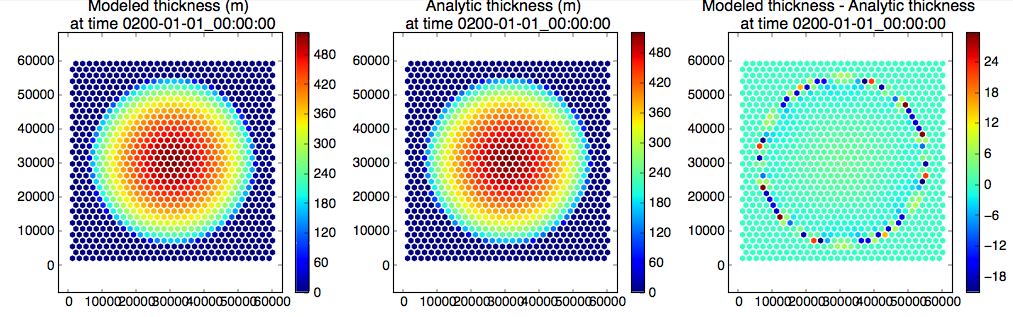
\includegraphics[width=16.4cm]{landice/figures/halfar.png}
	\caption{Halfar test case results after 200 years of dome evolution. This figure is generated by \texttt{halfar.py}.}
	\label{fig:halfarresults}
\end{figure}


\FloatBarrier

% ================================================================

\section{EISMINT-1 Test Cases}
\label{sec:eismint_description}
This test case is from the European Ice Sheet Modelling INiTiative intercomparison experiments.  These experiments are described at \url{http://homepages.vub.ac.be/~phuybrec/eismint.html} and in \citet{Huybrechts1996}.

Currently only the Moving Margin 1 Test Case from EISMINT-1 is included.


\subsection{Provided Files}
\label{subsec:eismint_files}


\begin{itemize}
\item namelist.landice: \\
	This file is used for actually running the dome test case in the MPAS land ice core.  It may not include all options available to the model.  See the namelist.landice.defaults file in the MPAS root directory for a list of all options available.  They are also documented in Chapter \ref{chap:namelist_tables}.

\item streams.landice: \\
	This file is used for specifying file input/output settings for the model.

\item check\_output\_eismint-mm1.py \\
This script can be used to compare model output to results from the EISMINT intercomparison.

\item namelist.input.periodic\_hex \\
 This file is used for running the grid generation tool \texttt{periodic\_hex} to create a grid for the test case.  It needs to be renamed to 'namelist.input' to run periodic\_hex) if mesh needs to be generated.  If you downloaded a tar archive of this test case, you do not need to create the mesh and can ignore this file.

\item setup\_initial\_conditions\_EISMINT1-MovingMargin-1.py \\
This file can be used to setup the initial conditions for the test case.  If you downloaded a tar archive, you do not need to do this.  However, if you want to modify the IC for some reason, you can edit and run this script.

\end{itemize}

\subsection{Results}
\label{subsecc:eismint_results}
As the initial ice sheet evolves, its shape eventually reaches a steady-state with the imposed surface mass balance.  
The script \texttt{check\_output\_eismint-mm1.py} will plot the modeled thickness at a specified time, 
as well as compare the model results to the results from the original EISMINT intercomparison.  
Invoke \texttt{check\_output\_eismint-mm1.py --help} for details of its usage.  
The script will compare the maximum ice thickness at the final time of the model output 
to the values reported from the models participating in the EISMINT-1 intercomparison.  
You should see something similar to this:

\begin{verbatim}
====================================
Max modeled thickness (m) = 2974.79474126
EISMINT models ice thickness at divide (m):
  3d models (10 of them): 2978.0 +/- 19.3
  2d models (3 of them):  2982.2 +/- 26.4
====================================
\end{verbatim}

% ================================================================


\section{Real World Test Cases}
Eventually grids for real-world Greenland and Antarctica will be provided at varying resolutions.



\chapter{Global Statistics}
\label{chap:global_statistics}

MPAS-Ocean simulations create global statistics text files that are accessible during the simulation, as described in Table \ref{oceanTable:global statistics}.  These are useful to check the health and progress of a simulation, and to compare the history of global statistics amongst similar simulations.  Frequency is controlled by \verb|_stats_| flags in the namelist.  The files are simply text files formatted in columns and rows, where each row is a particular time, written to \verb|stats_time.txt|, and each column is a variable, described in \verb|stats_readme.txt|.  Output is always appended to the {\tt stats\_*} files, so these files must be deleted or moved in order to restart from line one.

A chain of simple unix commands may be used to access a specific part of the data.  For example, to view the last three values of column seven in the global average, use
\begin{verbatim}
cat stats_avg.txt | awk '{print $7}' | tail -n3
\end{verbatim}
Gnuplot is a simple plotting tool available on Linux systems that can easily plot columns in text files.  In this example, two MPAS-Ocean simulations were executed, in directories \verb|run1| and \verb|run2|.  Begin Gnuplot with the \verb|gnuplot| command at the unix prompt.  Plot column seven from both runs using points with
\begin{verbatim}
plot 'run1/stats_avg.txt' u 7 w p, 'run2/stats_avg.txt' u 7 w p
\end{verbatim}
and with lines using
\begin{verbatim}
plot 'run1/stats_avg.txt' u 7 w l, 'run2/stats_avg.txt' u 7 w l
\end{verbatim}
Plot on a vertical log scale and add legend text with
\begin{verbatim}
set logscale y
plot 'run1/stats_avg.txt' u 7 w l t 'run 1', 'run2/stats_avg.txt' u 7 w l t 'run 2'
\end{verbatim}
It is often useful to view the difference between the global statistics of two simulations.  This can be done with the paste command, which concatenates the two files horizontally.  In this example, each file has 18 columns, so \$25 refers to column 7 of the second file:
\begin{verbatim}
plot '<paste run1/stats_avg.txt run2/stats_avg.txt' u ($7-$25)
\end{verbatim}

\begin{table}[ht] 
\caption{Global statistics output files.}
\vspace{0.5cm} \centering 
\begin{tabular}{ll} 
\hline\hline file name & description  \\
\hline 
\verb|stats_time.txt| & time stamp, rows correspond to rows of other stats files \\
\verb|stats_readme.txt| & list of variables in columns of other stats files \\
\verb|stats_min.txt| & minimum over the global domain \\
\verb|stats_max.txt| & maximum over the global domain \\
\verb|stats_sum.txt| & volume-weighted summation over the global domain \\
\verb|stats_avg.txt| & volume-weighted average over the global domain \\
\verb|stats_rms.txt| & volume-weighted root mean square over the global domain \\
\verb|stats_colmin.txt| & minimum column sum over the global domain \\
\verb|stats_colmax.txt| & maximum column sum over the global domain \\
\hline 
\end{tabular} \label{oceanTable:global statistics} 
\end{table}

\begin{figure}[H!]
	\centering
	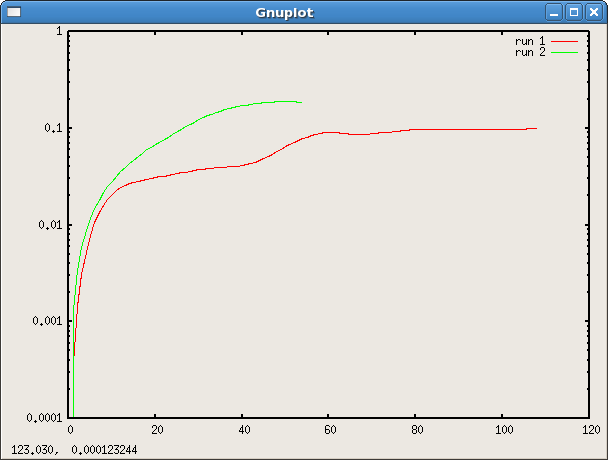
\includegraphics[scale=0.5]{ocean/figures/gnuplot.png}
	\caption{Example of plot of global statistics created with gnuplot.}
	\label{fig:gnuplot}
\end{figure}

\section{Surface-area average}
\label{sec:surface_area_average}

This analysis members computes areal-averages, areal-minimum and areal-maximum of two dimensional fields that are defined primarily at the surface. Let $R$ represent some subset to ocean surface cells and $f$ be some field defined on these ocean cells. Then the total area of region $R$ is given as

\begin{equation}
sumArea(R) = \sum_{i \in R} areaCell(i)
\end{equation}
where $i$ denotes any ocean surface cell and $areaCell(i)$ is the area of that cell. For any function $f$ defined at ocean surface cells we have

\begin{equation}
avg(f(R)) = \frac{\sum_{i \in R} f(i)*areaCell(i)}{sumArea(R)}
\end{equation}

In addition to computing averages, the analysis member also computes the minimum and maximum values of $f$ with region $R$ as

\begin{equation}
minval(f(R))=min(f(i)) \, \, \forall i \in R
\end{equation}
\begin{equation}
maxval(f(R))=max(f(i)) \, \, \forall i \in R
\end{equation}

{\noindent}To be added to AM before release 5.0 .....\\
The region $R$ is defined using surfaceRegionMask that have values of 0 for cells not in region $R$ and a values of 1 for cells within region $R$. As a result, the analysis member operates on an arbitrary number regions.

\section{Layer-volume-average}
\label{sec:layer_volume_average}

This analysis members computes areal-averages, areal-minimum and areal-maximum of three dimensional fields at each vertical level. Except for the loop over the vertical index $k$, this analysis member is self-similar to that described in Section \ref{sec:surface_area_average}. As the vertical index increases, the area associated with the region might reduce. Let $R$ contain the cells within some subset to ocean surface cells and $R(k)$ to contain the ocean cells that are contained in $R$ at vertical index $k$. Then the total volume of region $R(k)$ is given as

\begin{equation}
sumVolume(R(k)) = \sum_{i \in R \,\, \& \,\, k \le maxLevelCell(i)} layerThickness(k,i) * areaCell(i)
\end{equation}
where $i$ denotes any ocean surface cell, $areaCell(i)$ is the area of that cell and $maxLevelCell(i)$ is the vertical depth of cell $i$ measured in index space. The variable $layerThickness$ represent the vertical depth of cell $i$ at depth $k$.

For any function $g(k,i)$ representing a 3D field (e.g. temperature) we have

\begin{equation}
avg(g(R(k))) = \sum_{i \in R \,\, \& \,\, k \le maxLevelCell(i)} g(k,i)*layerThickness(i,k)*areaCell(i) / sumVolume(R(k))
\end{equation}

In addition to computing averages for each region at each depth index, the analysis member also computes the minimum and maximum values of $g$ with region $R(k)$ as

\begin{equation}
minval(g(R))=min(g(i)) \, \, \forall i \in R \,\, \& \,\, k \le maxLevelCell(i)
\end{equation}
\begin{equation}
maxval(g(R))=max(g(i)) \, \, \forall i \in R \,\, \& \,\, k \le maxLevelCell(i)
\end{equation}

{\noindent}To be added to AM before release 5.0 .....\\
The region $R$ is defined using surfaceRegionMask that has values of 0 for cells not in region $R$ and a values of 1 for cells within region $R$. As a result, the analysis member operates on an arbitrary number regions.


\chapter{Analysis Mode}
\label{chap:analysis_mode}
\renewcommand{\mode}{analysis}
\section{Purpose}

\section{Compilation}



\section{Dimensions}
\label{sec:analysis_dimensions}
{\small
\begin{center}
\begin{longtable}{| p{1.0in} || p{1.0in} | p{4.0in} |}
	\hline 
	{\bf Name} & {\bf Units} & {\bf Description} \endfirsthead
	\hline 
	{\bf Name} & {\bf Units} & {\bf Description} (Continued) \endhead
	\hline 
	\hline 
	nCells & $unitless$ & The number of polygons in the primary grid. \\ 
	\hline
	nEdges & $unitless$ & The number of edge midpoints in either the primary or dual grid. \\ 
	\hline
	maxEdges & $unitless$ & The largest number of edges any polygon within the grid has. \\ 
	\hline
	maxEdges2 & $unitless$ & Two times the largest number of edges any polygon within the grid has. \\ 
	\hline
	nAdvectionCells & $unitless$ & The largest number of advection cells for any edge. \\ 
	\hline
	nVertices & $unitless$ & The total number of cells in the dual grid. Also the number of corners in the primary grid. \\ 
	\hline
	TWO & $unitless$ & The number two as a dimension. \\ 
	\hline
	R3 & $unitless$ & The number three as a dimension. \\ 
	\hline
	SIX & $unitless$ & The number six as a dimension. \\ 
	\hline
	FIFTEEN & $unitless$ & The number 15 as a dimension. \\ 
	\hline
	TWENTYONE & $unitless$ & The number 21 as a dimension. \\ 
	\hline
	vertexDegree & $unitless$ & The number of cells or edges touching each vertex. \\ 
	\hline
	nVertLevels & $unitless$ & The number of levels in the vertical direction. All vertical levels share the same horizontal locations. \\ 
	\hline
	nVertLevelsP1 & $unitless$ & The number of interfaces in the vertical direction. \\ 
	\hline
\end{longtable}
\end{center}
}
\section[Namelist options]{\hyperref[chap:namelist_sections]{Namelist options}}
\label{sec:analysis_namelist_tables}
Embedded links point to more detailed namelist information in the appendix.
\subsection[time\_management]{time\_management}
\label{subsec:analysis_nm_tab_time_management}
General time management is handled by the time\_management namelist record.
Included options handle time-related parts of MPAS, such as the calendar and if the simulation is a restart or not.

Users should use this record to specify the beginning time of the simulation,
and either the duration or the end of the simulation. Only the end or the
duration need to be specified as the other is derived within MPAS from the
beginning time and other specified one.

{\bf TBA: If both duration and stop are specified, then what happens?)}

\vspace{0.5in}
{\small
\begin{center}
\begin{longtable}{| p{2.0in} || p{4.0in} |}
	\hline
	{\bf Name} & {\bf Description} \endfirsthead
	\hline 
	{\bf Name} & {\bf Description} (Continued) \endhead
	\hline
	\hline
	\hyperref[sec:nm_sec_config_do_restart]{config\_do\_restart} & Determines if the initial conditions should be read from a restart file, or an input file. \\
	\hline
	\hyperref[sec:nm_sec_config_start_time]{config\_start\_time} & Timestamp describing the initial time of the simulation. If it is set to 'file', the initial time is read from restart\_timestamp. \\
	\hline
	\hyperref[sec:nm_sec_config_stop_time]{config\_stop\_time} & Timestamp descriping the final time of the simulation. If it is set to 'none' the final time is determined from config\_start\_time and config\_run\_duration. \\
	\hline
	\hyperref[sec:nm_sec_config_run_duration]{config\_run\_duration} & Timestamp describing the length of the simulation. If it is set to 'none' the duration is determined from config\_start\_time and config\_stop\_time. config\_run\_duration overrides inconsistent values of config\_stop\_time. \\
	\hline
	\hyperref[sec:nm_sec_config_calendar_type]{config\_calendar\_type} & Selection of the type of calendar that should be used in the simulation. \\
	\hline
\end{longtable}
\end{center}
}
\subsection[io]{io}
\label{subsec:analysis_nm_tab_io}
The io namelist record provides options for modifications to the I/O system of
MPAS. These include frequency, file name, and parallelization options.

\vspace{0.5in}
{\small
\begin{center}
\begin{longtable}{| p{2.0in} || p{4.0in} |}
	\hline
	{\bf Name} & {\bf Description} \endfirsthead
	\hline 
	{\bf Name} & {\bf Description} (Continued) \endhead
	\hline
	\hline
	\hyperref[sec:nm_sec_config_input_name]{config\_input\_name} & The path to the input file for the simulation. \\
	\hline
	\hyperref[sec:nm_sec_config_output_name]{config\_output\_name} & The template path and name to the output file from the simulation. A time stamp is prepended to the extension of the file (.nc). \\
	\hline
	\hyperref[sec:nm_sec_config_restart_name]{config\_restart\_name} & The template path and name to the restart file for the simulation. A time stamp is prepended to the extension of the file (.nc) both for input and output. \\
	\hline
	\hyperref[sec:nm_sec_config_restart_timestamp_name]{config\_restart\_timestamp\_name} & The name of the file timestamps for latest restart files are written to. This file is also read when config\_start\_time is set to 'file' and config\_do\_restart is set to .true. \\
	\hline
	\hyperref[sec:nm_sec_config_restart_interval]{config\_restart\_interval} & Timestamp determining how often a restart file should be written. \\
	\hline
	\hyperref[sec:nm_sec_config_output_interval]{config\_output\_interval} & Timestamp determining how often an output file should be written. \\
	\hline
	\hyperref[sec:nm_sec_config_stats_interval]{config\_stats\_interval} & Timestamp determining how often a global statistics files should be written. \\
	\hline
	\hyperref[sec:nm_sec_config_write_stats_on_startup]{config\_write\_stats\_on\_startup} & Logical flag determining if statistics files should be written prior to the first time step. \\
	\hline
	\hyperref[sec:nm_sec_config_write_output_on_startup]{config\_write\_output\_on\_startu-}\hyperref[sec:nm_sec_config_write_output_on_startup]{p}& Logical flag determining if an output file should be written prior to the first time step. \\
	\hline
	\hyperref[sec:nm_sec_config_frames_per_outfile]{config\_frames\_per\_outfile} & Integer specifying how many time frames should be included in an output file. Once the maximum is reached, a new output file is created. \\
	\hline
	\hyperref[sec:nm_sec_config_pio_num_iotasks]{config\_pio\_num\_iotasks} & Integer specifying how many IO tasks should be used within the PIO library. A value of 0 causes all MPI tasks to also be IO tasks. IO tasks are requried to write contiguous blocks of data to a file. \\
	\hline
	\hyperref[sec:nm_sec_config_pio_stride]{config\_pio\_stride} & Integer specifying the stride of each IO task. \\
	\hline
\end{longtable}
\end{center}
}
\subsection[time\_integration]{time\_integration}
\label{subsec:analysis_nm_tab_time_integration}
The time integration namelist controls parameters that pertain to all time-stepping methods.  At present, Forward Euler is the only time integration method implemented.

\vspace{0.5in}
{\small
\begin{center}
\begin{longtable}{| p{2.0in} || p{4.0in} |}
	\hline
	{\bf Name} & {\bf Description} \endfirsthead
	\hline 
	{\bf Name} & {\bf Description} (Continued) \endhead
	\hline
	\hline
	\hyperref[sec:nm_sec_config_dt]{config\_dt} & Length of model time-step. \\
	\hline
	\hyperref[sec:nm_sec_config_time_integrator]{config\_time\_integrator} & Time integration method. \\
	\hline
\end{longtable}
\end{center}
}
\subsection[ALE\_vertical\_grid]{ALE\_vertical\_grid}
\label{subsec:analysis_nm_tab_ALE_vertical_grid}
The MPAS-Ocean vertical grid is structured arbitrary Lagrangian-Eulerian (ALE).   ALE provides a great deal of freedom in the choice of vertical coordinate: when fully Eulerian, MPAS-Ocean is a z-level model with fixed thicknesses; when fully Lagrangian, there is no vertical transport between layers, and layers expand and contract like an isopycnal ocean model.  In between are many additional options, such as z-star where layers expand in proportion to the sea surface height, and sigma, where coordinates are terrain-following.

MPAS-Ocean employs the continuity equation,
\begin{eqnarray}
\label{ocean:continuity thickness}
\frac{\partial h_{k}}{\partial t} + D_k + w^t_k - w^t_{k+1} =0
\end{eqnarray}
for the ALE formulation, where variables are defined in Table \ref{oceanTable:ALE_variables}.  The ALE algorithm is as follows:
\begin{enumerate}
\item ALE step: Compute desired thickness for the new time,
\begin{eqnarray}
\label{ocean:desired thickness}
h_k^{ALE} = h_k^{rest} + h_k^{SSH} + h_k^{hf} + h_k^{min}
\end{eqnarray}
\item ALE step: Solve for vertical transport $w^t$ from (\ref{ocean:continuity thickness}),
\begin{eqnarray}
\label{ocean:vert tranport}
w^t_k = w^t_{k+1} - D_k - \frac{h^{ALE}_k - h^n_k}{\Delta t}
\end{eqnarray}
\item Solve for new thickness, $h_{k}^{n+1}$, using the continuity equation (\ref{ocean:continuity thickness}) within the time integration routine.
\end{enumerate}
The redundancy in steps 2 and 3 are intentional, so that step 2 is isolated within the ALE subroutine, and step 3 is solved in the timestepping subroutine in the identical manner as the tracer equation (\ref{ocean:tracer}).

The desired ALE thickness includes contributions from four terms (\ref{ocean:desired thickness}):
\begin{enumerate}
\item {\bf Resting thickness}, $h^{rest}$, is the layer thickness when the ocean is at rest, i.e. without SSH or internal perturbations.  For z-type coordinates, the resting thickness is constant in each horizontal layer.
\item {\bf SSH alteration}, $h^{SSH}$, alters layer thicknesses so that they change in proportion to the sea surface height (SSH),
\begin{eqnarray}
\label{ocean:h ssh}
   h_k^{SSH} =  \zeta \frac{W_k h^{rest}_k}{\sum_{k'=1}^{kmax}W_{k'}h^{rest}_{k'}}
\end{eqnarray}
The weights $W_k$ determine how SSH oscillations are distributed amongst the layers, as described in Table \ref{oceanTable:vertical coordinates}.
\item {\bf High-frequency thickness}, $h^{hf}$, allows high-frequency thickness oscillations, such as internal gravity waves, to be treated in a Lagrangian manner.  This is the ``z-tilde'' scheme of \citet{Leclair_Madec11om} described in the next section.
\item {\bf Minimum thickness alteration}, $h^{min}$, is the change in thickness required to enforce the minimum thickness in each cell.  When a cell is too thin, $h^{min}$ is positive, while nearby cells in the vertical incur a corresponding negative $h^{min}$ to conserve volume in the column.
\end{enumerate}
Of the four terms, resting thickness is always positive, while the others are small alterations about zero.  Summing a column,
\begin{eqnarray}
\sum_{k=1}^{kmax} h_k^{ALE} &=& \sum_{k=1}^{kmax} h_k^{rest} + \sum_{k=1}^{kmax}h_k^{SSH} + \sum_{k=1}^{kmax}h_k^{hf} + \sum_{k=1}^{kmax}h_k^{min} 
\nonumber \\
&=& H + \zeta + 0 + 0.
\nonumber
\end{eqnarray}
Thus the first two terms are always included so that the column thickness sums to $H+\zeta$, while the second two terms are optional and may be turned on with flags.

In order to assist users in choosing the correct settings, we provide a description of traditional vertical coordinate names in Table \ref{oceanTable:vertical coordinates}.
The vertical coordinate type also depends upon the set-up of the layerThickness variable in the initial condition file.  For all Z-type vertical coordinates, initial layer thicknesses are horizontally constant.  For sigma coordinates, layers are terrain-following and all layers are employed.  In this case, the user may still choose amongst the flags in SSH may be distributed through the column just like with z-type models in Table \ref{oceanTable:vertical coordinates}.

In order to run an isopycnal configuration, use config\_vert\_coord\_movement='impermeable\_interfaces' and set initial temperature and salinity to be constant within each layer.  All vertical tracer diffusion must be off so that the density in each layer remains constant.  For an isopycnal set-up, the equation of state is still called at each timestep, so a linear equation of state is recommended to avoid depth-dependancy of the density.  The user may choose a Montgomery Potential (\ref{ocean:Montgomery Potential}) or standard pressure gradient (\ref{ocean:grad p}); Montgomery Potential is a more common choice for isopycnal configurations, but both are tested and functional.  MPAS-Ocean does not support massless layers at this time, so isopycnal vertical coordinates may only be used for idealized domains.

\begin{table}[ht] 
\caption{Vertical coordinate settings for traditional names.}
\vspace{0.5cm} \centering 
\begin{tabular}{c c c c c c} 
\hline\hline flag name &  {\bf Z-Level} & {\bf Z-star} & {\bf weighted Z-star} &  {\bf isopycnal}  \\
\hline 
config\_vert\_ & 'fixed' & 'uniform\_stretching' & 'user\_specified' & 'impermeable\_ \\
coord\_movement & & & & interfaces'
\\
weights & $W_k =\left\{ \begin{array}{c} 1\; k=1\\ 0\; k>1 \end{array}\right.$ & $W_k=1\;\;\forall\;\;k$ & input file & not applicable \\
\hline 
\end{tabular} \label{oceanTable:vertical coordinates} 
\end{table}

\begin{table}[h!t] 
\caption{Variables used in ALE equation sets.  Column 3 shows the native horizontal grid location.  A subscript $k$ indicates indicates the layer index.  The $\nabla$ indicates a horizontal gradient within a single layer.} 
\vspace{0.5cm} \centering 
\begin{tabular}{c c c c } 
\hline\hline symbol &  name & grid &  notes  \\
\hline 
$D$  & thickness-weighted divergence & cell & $D_k = \nabla \cdot  \left( h_k {\bf u}_k \right)$  \\ 
${\bar D}$ & barotropic divergence & cell & ${\overline D} = \sum\limits_{k=1}^{kmax} D_k$  \\ 
$D'$  & baroclinic divergence & cell & $D'_k = D_k-\frac{h_k}{H}{\bar D}$  \\ 
$D^{lf}$  & low-frequency divergence & cell & see (\ref{ocean:Dlf})  \\ 
$D^{hf}$  & high-frequency divergence & cell & $D^{hf}_k = D'_k - D^{lf}_k$  \\ 
$h$  & layer thickness & cell &   \\ 
$h^{ALE}$  & desired ALE thickness & cell & see (\ref{ocean:desired thickness})  \\ 
$h^{rest}$  & resting thickness & cell &   \\ 
$h^{SSH}$  & SSH thickness alteration & cell & see (\ref{ocean:h ssh})  \\ 
$h^{hf}$  & high-freq. thickness alteration & cell &   see (\ref{ocean:hhf})  \\ 
$h^{min}$  & minimum thickness alteration & cell &   \\ 
$H$  & total resting thickness & cell & $H= \sum\limits_{k=1}^{kmax} h_k^{rest}$  \\ 
${\bf u}$  & velocity & edge &   \\ 
$w^t$ & vertical transport & cell  & top of layer in vertical \\
$W$  & SSH thickness weights & cell &   \\ 
$\tau_{Dlf}$  & frequency filter time scale & constant &   \\ 
$\tau_{hhf}$  & restoring time scale for $h^{hf}$ & constant &   \\ 
$\kappa_{hhf}$  & $h^{hf}$ diffusion & constant &   \\ 
$\zeta$  & sea surface height & cell &  $\zeta= \sum\limits_{k=1}^{kmax} h_k^{rest} - H$  \\ 
\hline 
\end{tabular} \label{oceanTable:ALE_variables} 
\end{table}


\vspace{0.5in}
{\small
\begin{center}
\begin{longtable}{| p{2.0in} || p{4.0in} |}
	\hline
	{\bf Name} & {\bf Description} \endfirsthead
	\hline 
	{\bf Name} & {\bf Description} (Continued) \endhead
	\hline
	\hline
	\hyperref[sec:nm_sec_config_vert_coord_movement]{config\_vert\_coord\_movement} &  Determines the vertical coordinate movement type. 'uniform\_stretching' distributes SSH perturbations through all vertical levels (z-star vertical coordinate); 'fixed' places them all in the top level (z-level vertical coordinate); 'user\_specified' allows the input file to determine the distribution using the variable vertCoordMovementWeights (weighted z-star vertical coordinate); and 'impermeable\_interfaces' makes the vertical transport between layers zero, i.e.  $w^t=0$  in (\ref{ocean:vert tranport}) (idealized isopycnal). \\
	\hline
	\hyperref[sec:nm_sec_config_use_min_max_thickness]{config\_use\_min\_max\_thickness} & If true, a minimum and maximum thicknesses are enforced to prevent massless and very thick layers. \\
	\hline
	\hyperref[sec:nm_sec_config_min_thickness]{config\_min\_thickness} & Minimum thickness allowed. \\
	\hline
	\hyperref[sec:nm_sec_config_max_thickness_factor]{config\_max\_thickness\_factor} &  Maximum thickness allowed.  This is a factor times the resting thickness, i.e., maximum thickness = config\_max\_thickness\_factor* $h^{rest}$ . \\
	\hline
	\hyperref[sec:nm_sec_config_set_restingThickness_to_IC]{config\_set\_restingThickness\_t-}\hyperref[sec:nm_sec_config_set_restingThickness_to_IC]{o\_IC}& If true, set restingThickness to be the same as layerThickness upon start-up.  This only occurs when config\_do\_restart is false, i.e. on an initial run. \\
	\hline
	\hyperref[sec:nm_sec_config_dzdk_positive]{config\_dzdk\_positive} & Determines if the positive Z axis is aligned with the positive K index direction. \\
	\hline
\end{longtable}
\end{center}
}
\subsection[ALE\_frequency\_filtered\_thickness]{ALE\_frequency\_filtered\_thickness}
\label{subsec:analysis_nm_tab_ALE_frequency_filtered_thickness}
The high-frequency thickness alteration, $h^{hf}$, in (\ref{ocean:\mode_desired thickness}) allows the thicknesses to oscillate so that high-frequency motions, such as internal gravity waves, are treated in a Lagrangian manner.  Low-freqency motions, such as seasonal changes or slow motions of water masses, are treated in an Eulerian manner.  This is the ``z-tilde'' scheme of \citet{Leclair_Madec11om}, which generally reduces spurious vertical mixing and preserves water mass properties.  Two additional prognostic equations are solved when config\_use\_freq\_filtered\_thickness is true,
\begin{eqnarray}
\label{ocean:\mode_Dlf}
 & \displaystyle
  \frac{\partial D^{lf}_k}{\partial t} = - \frac{2\pi}{\tau_{Dlf}} \left( D^{lf}_k - D'_k \right), 
\\ & \displaystyle
\label{ocean:\mode_hhf}
\frac{\partial h^{hf}_k}{\partial t} =  - D^{hf}_k - \frac{2\pi}{\tau_{hhf}} h^{hf}_k + \nabla_h\cdot \left( \kappa_{hhf} \nabla_h h^{hf}_k \right) 
\end{eqnarray}
where $\tau_{Dlf}$ is the filter timescale and other variables are defined in Table \ref{oceanTable:\mode_ALE_variables}.  This may be used in addition to any of the z-type or sigma-type vertical coordinates in Table \ref{oceanTable:\mode_vertical coordinates}.  Some combination of thickness restoring and diffusion are recommended to avoid long-term drift of $h^{hf}$ away from zero.




\vspace{0.5in}
{\small
\begin{center}
\begin{longtable}{| p{2.0in} || p{4.0in} |}
	\hline
	{\bf Name} & {\bf Description} \endfirsthead
	\hline 
	{\bf Name} & {\bf Description} (Continued) \endhead
	\hline
	\hline
	\hyperref[sec:nm_sec_config_use_freq_filtered_thickness]{config\_use\_freq\_filtered\_thickn-}\hyperref[sec:nm_sec_config_use_freq_filtered_thickness]{ess}&  If true,  $h^{hf}$  is included in the desired ALE thickness in \ref{ocean:desired thickness}, and the prognostic equations \ref{ocean:Dlf} and \ref{ocean:hhf} are integrated in the code. \\
	\hline
	\hyperref[sec:nm_sec_config_thickness_filter_timescale]{config\_thickness\_filter\_timescal-}\hyperref[sec:nm_sec_config_thickness_filter_timescale]{e}&  Filter time scale for the low-frequency baroclinic divergence,  $\tau_{Dlf}$ . \\
	\hline
	\hyperref[sec:nm_sec_config_use_highFreqThick_restore]{config\_use\_highFreqThick\_rest-}\hyperref[sec:nm_sec_config_use_highFreqThick_restore]{ore}&  If true, the high frequency thickness equation (\ref{ocean:hhf}) includes term 2 on the RHS, the restoring term.  The high frequency thickness is restored to zero with time scale  $\tau_{hhf}$ . \\
	\hline
	\hyperref[sec:nm_sec_config_highFreqThick_restore_time]{config\_highFreqThick\_restore\_-}\hyperref[sec:nm_sec_config_highFreqThick_restore_time]{time}&  Restoring time scale for high-frequency thickness,  $\tau_{hhf}$ . \\
	\hline
	\hyperref[sec:nm_sec_config_use_highFreqThick_del2]{config\_use\_highFreqThick\_del2} & If true, high frequency thickness equation (\ref{ocean:hhf}) includes term 3 on the RHS, the diffusion term. \\
	\hline
	\hyperref[sec:nm_sec_config_highFreqThick_del2]{config\_highFreqThick\_del2} &  Horizonal high frequency thickness diffusion,  $\kappa_{hhf}$ . \\
	\hline
\end{longtable}
\end{center}
}
\subsection[partial\_bottom\_cells]{partial\_bottom\_cells}
\label{subsec:analysis_nm_tab_partial_bottom_cells}
\documentclass[11pt]{report}

\usepackage{epsf,amsmath,amsfonts}
\usepackage{graphicx}

\setlength{\textwidth}{6.5in}
\setlength{\oddsidemargin}{0in}
\setlength{\evensidemargin}{0in}
\setlength{\textheight}{8.5in}
\setlength{\topmargin}{0in}

\begin{document}

\title{
Requirements and Design\\
Partial Bottom Cells}
\author{MPAS Development Team}

\maketitle
\tableofcontents

%-----------------------------------------------------------------------

\chapter{Summary}

Partial bottom cells (PBCs) allow bottom topography to be represented more realistically.  Currently, MPAS-Ocean only suports full ocean cells, so the bottom depth of a column is restricted to the depth of each vertical cell interface.  With partial bottom cells, the bottom depth may take on any value.  This is still a z-level-type formulation, where cells that are fully below the bottom depth are considered land cells.  The PBC formulation will work with z-level, z-star, and z-tilde formulations.

%figure template
%\begin{figure}
%  \center{\includegraphics[width=14cm]{./Figure1.pdf}}
%  \caption{A graphical representation of the discrete boundary.}
%  \label{Figure1}
%\end{figure} 

%-----------------------------------------------------------------------

\chapter{Requirements}

\section{Requirement: initial conditions with consistant variables}
Date last modified: 2012/10/15 \\
Contributors: Mark Petersen \\

The following variables must be consistent upon starting a new simulation with mpas-ocean: bottomDepth, maxLevelCell, thickness $h$, location of initial tracers in bottom cell.

\section{Requirement: horizontal advection}
Date last modified: 2012/08/01 \\
Contributors: Mark Petersen \\

Horizontal advection must take place through a thickness that accounts for the partial bottom cell at the bottom of the column.

\section{Requirement: pressure gradient}
Date last modified: 2012/08/01 \\
Contributors: Mark Petersen \\

Pressure gradients must not contain spurious effects due to the partial bottom cells.



%-----------------------------------------------------------------------

\chapter{Algorithmic Formulations}

\section{Design Solution: initial conditions with consistant variables}

Date last modified: 2012/10/15 \\
Contributors: Mark Petersen \\

The thickness variable {\tt h(k,iCell,iStep)} will continue to be the actual thickness of fluid in the cell.  
A new variable, {\tt bottomDepth(iCell)}, is the depth below the average sea surface height ($z=0$) in each cell, and is a positive number.    The variable {\tt maxLevelCell(iCell)} is an integer of the deepest active (water-filled) cell, and {\tt refBottomDepth(k)} is the depth of the bottom of each cell in z-level coordinates.  Note that depth variables are positive, $z$ variables are negative and decrease with greater depths, and the $k$ index increases with greater depth.

In generating the initial conditions (IC), the following steps are taken:
\begin{enumerate}
\item An additional parameter, {\tt max\_partial\_bottom\_cell}, may be set between zero and one, with default .95, in the initial condition generation.  Then {\tt bottomDepth} must be altered so that a partial bottom cell has a maximum of (say) 95\% land.  This parameter may be adjusted after testing. 
\item The thickness {\tt h} at {\tt k=maxLevelCell} is reduced to take into account the thickness removed by the partial bottom cell.
\item Initial tracer values in the bottom cell are interpolated to the center of the pbc, rather than the center of the full cell.
\item Check that {\tt bottomDepth} corresponds to {\tt maxLevelCell} (because they are redundant):\\
when {\tt k=maxLevelCell(iCell)}:\\
{\tt refBottomDepth(k)<bottomDepth(iCell)< refBottomDepth(k-1)}
\end{enumerate}

The ICs could be altered in basin.F or upon start-up with mpas.  We chose to alter the ICs in mpas to reduce the number and IC files and the complexity of IC generation.  The initial netcdf file (ocean.nc, produced by basin), include a realistic
 bottomDepth variable and thickness and tracer variables for full thickness cells.

Upon start-up with {\tt config\_do\_restart = .false.}, ICs are altered as described above.  An additional flag is used as follows:
\begin{itemize}
\item If running with pbcs, set {\tt config\_alter\_ICs\_for\_pbc='zlevel\_pbcs\_on'}. Then thin pbc cells
   will be changed, and thickness and tracers will be altered to match the pbcs (steps 1-3, above).
\item If running without pbcs, set {\tt config\_alter\_ICs\_for\_pbc='zlevel\_pbcs\_off'}. Then 
   bottomDepth will be altered so it is full cells everywhere.
   If your input file does not include bottomDepth, the false option will
   initialize bottomDepth correctly for a non-pbc run.
\item Set {\tt config\_alter\_ICs\_for\_pbc='no'} for isopycnal or sigma coordinates.
\end{itemize}

Consistency between {\tt bottomDepth} and {\tt maxLevelCell} is verified afterwards if {\tt config\_check\_zlevel\_consistency=.true.}


\section{Design Solution: horizontal advection}
Date last modified: 2012/08/01 \\
Contributors: Mark Petersen \\

{\bf Option 1: Do nothing (this option was chosen)}\\

If nothing is changed in the current code, {\tt h\_edge} is computed from from the thickness of nearby cells, regardless of PBCs in the bottom layer.  This is a clean and simple solution, but if PBCs are very thin, a cell could be evacuated of water.\\

{\bf Option 2: h\_edge is limited by minimum depth of neighboring cells}\\

In POP, the thickness of a U-cell is the minimum of the four surrounding T-Cells.  Likewise in MPAS-Ocean, one could compute the edge thickness using the minimum bottom depth of the two surrounding cells.  For the computation of {\tt h\_edge} using higher order advection methods, this will require further thought.

\section{Design Solution: pressure gradient}
Date last modified: 2012/08/01 \\
Contributors: Mark Petersen \\

{\bf Option 1: Do nothing (this option was chosen)}\\

MPAS-Ocean currently has two terms related to the pressure gradient,
\begin{equation}
- \frac{1}{\rho_0}\nabla p_k  - \frac{\rho g}{\rho_0}\nabla z^{mid}_k.
\end{equation}
where the gradient of $z^{mid}$ makes up pressure differences due to tilted levels.  However, in a stratified ocean, pressure gradient errors occur when the tilting of levels is large.  In a z-star system without PBCs, these perturbations are limited by the ratio of sea surface height to total depth, so only a few percent.  With the inclusion of PBCs, $z^{mid}$ could vary from one gridcell to the next by half the layer thickness.\\

{\bf Option 2: Interpolate T \& S to center of bottom cell for pressure computation}\\

If the pressure gradient errors are deemed to be too large, one could extrapolate the temperature and salinity values to the mid-depth of the bottom cell, and compute density and pressure at that location.  This will require a special case when {\tt k=maxLevelCell}.  There will need to be an extra case in the computation of $\nabla z^{mid}$ as well, so that $z^{mid}$ at the bottom cell is at the cell center.


%-----------------------------------------------------------------------

\chapter{Design and Implementation}

\section{Implementation: consistency between thickness and partial bottom cell variables}
Date last modified: 2012/08/01 \\
Contributors: Mark Petersen \\


\section{Implementation: horizontal advection}
Date last modified: 2012/08/01 \\
Contributors: Mark Petersen \\


\section{Implementation: pressure gradient}
Date last modified: 2012/08/01 \\
Contributors: Mark Petersen \\


%-----------------------------------------------------------------------

\chapter{Testing}

\section{Testing and Validation: Partial bottom cells}
Date last modified: 2012/08/01 \\
Contributors: Mark Petersen \\

Use the test problem, already in the repository, following Ilicak ea 2012 overflow test case (\#4).


%-----------------------------------------------------------------------

\end{document}

\vspace{0.5in}
{\small
\begin{center}
\begin{longtable}{| p{2.0in} || p{4.0in} |}
	\hline
	{\bf Name} & {\bf Description} \endfirsthead
	\hline 
	{\bf Name} & {\bf Description} (Continued) \endhead
	\hline
	\hline
	\hyperref[sec:nm_sec_config_alter_ICs_for_pbcs]{config\_alter\_ICs\_for\_pbcs} & If true, initial conditions are altered according to the config\_pbc\_alteration\_type flag.  The alteration of layer thickness only occurs when config\_do\_restart is false, i.e. on an initial run. \\
	\hline
	\hyperref[sec:nm_sec_config_pbc_alteration_type]{config\_pbc\_alteration\_type} & Determines the method of initial condition alteration for partial bottom cells.  'partial\_cell' alters layerThickness, interpolates all tracers in the bottom cell based on the bottomDepth variable, and alters bottomDepth to enforce the minimum pbc fraction.  'full\_cell' alters bottomDepth to have full cells everywhere, based on the refBottomDepth variable. \\
	\hline
	\hyperref[sec:nm_sec_config_min_pbc_fraction]{config\_min\_pbc\_fraction} & Determines the minimum fraction of a cell altering the initial conditions can create.  The alteration of layer thickness only occurs when config\_do\_restart is false, i.e. on an initial run. \\
	\hline
	\hyperref[sec:nm_sec_config_check_ssh_consistency]{config\_check\_ssh\_consistency} & Enables a check to determine if the SSH is within 2m of the surface, as specified in (\ref{ocean:pbc SSH}). \\
	\hline
\end{longtable}
\end{center}
}
\subsection[decomposition]{decomposition}
\label{subsec:analysis_nm_tab_decomposition}
MPAS handles decomposing all variables into computational blocks. The
decomposition used needs to be specified at run time and is computed by an
external tool (e.g. metis). Additionally, MPAS supports multiple computational
blocks per MPI process, and the user may specify an additional decomposition
file which can specify the assignment of blocks to MPI processes. Run-time
parameters that control the run-time decomposition used are specified within
the decomposition namelist record.


\vspace{0.5in}
{\small
\begin{center}
\begin{longtable}{| p{2.0in} || p{4.0in} |}
	\hline
	{\bf Name} & {\bf Description} \endfirsthead
	\hline 
	{\bf Name} & {\bf Description} (Continued) \endhead
	\hline
	\hline
	\hyperref[sec:nm_sec_config_num_halos]{config\_num\_halos} & Determines the number of halo cells extending from a blocks owned cells (Called the 0-Halo). The default of 3 is the minimum that can be used with monotonic advection. \\
	\hline
	\hyperref[sec:nm_sec_config_block_decomp_file_prefix]{config\_block\_decomp\_file\_prefix} & Defines the prefix for the block decomposition file. Can include a path. The number of blocks is appended to the end of the prefix at run-time. \\
	\hline
	\hyperref[sec:nm_sec_config_number_of_blocks]{config\_number\_of\_blocks} & Determines the number of blocks a simulation should be run with. If it is set to 0, the number of blocks is the same as the number of MPI tasks at run-time. \\
	\hline
	\hyperref[sec:nm_sec_config_explicit_proc_decomp]{config\_explicit\_proc\_decomp} & Determines if an explicit processor decomposition should be used. This is only useful if multiple blocks per processor are used. \\
	\hline
	\hyperref[sec:nm_sec_config_proc_decomp_file_prefix]{config\_proc\_decomp\_file\_prefix} & Defines the prefix for the processor decomposition file. This file is only read if config\_explicit\_proc\_decomp is .true. The number of processors is appended to the end of the prefix at run-time. \\
	\hline
\end{longtable}
\end{center}
}
\subsection[hmix]{hmix}
\label{subsec:analysis_nm_tab_hmix}
There are several choices of horizontal mixing schemes available for the 
momentum and tracer equations.  Each of these is a turbulence closure, 
and attempts to account for subgrid-scale mixing and diffusion.  These 
schemes have the practical effect of reducing grid-scale noise in the 
velocity and tracer fields, and improving numerical stability.

Each horizontal mixing scheme has its own namelist, and may be turned
on with the \verb|_use_| logical configuration flags.  Multiple
schemes may be run simultaneously.  The horizontal mixing terms in the
governing equations (\ref{ocean:momentum},
\ref{ocean:tracer}) are ${\bf D}^u_h$ for momentum and
$D^\varphi_h$ for tracers.  No horizontal mixing is applied to the
thickness equation.

All horizontal mixing coefficients can be set to scale with the mesh as $\rho_m^{-3/4}$ in equations (\ref{ocean:\mode_h_mom_del2}, \ref{ocean:\mode_h_tr_del2}, \ref{ocean:\mode_h_mom_del4}, \ref{ocean:\mode_h_tr_del4}).  The mesh density, $\rho_m$, is a variable in the input and restart file.  It can vary between zero and one, and is one in the highest resolution region.  Scaling with the mesh can be turned off, as described in the options below.

The anticipated potential Vorticity (APV) method is a parameterization of the effects of subgrid or unresolved scales on those explicitly resolved \citep{Vallis_Hua88jas}.  It contributes an upstream bias to the vorticity in the del2 and del4 momentum terms as follows,
\begin{equation}
\eta_{apv} = \eta - c_{apv} dt \left({\bf u}\cdot \nabla \eta\right),
\end{equation}
where the altered vorticity $\eta_{apv}$ is used in equations (\ref{ocean:\mode_h_mom_del2}, \ref{ocean:\mode_h_mom_del4a}, \ref{ocean:\mode_h_mom_del4b}).

\vspace{0.5in}
{\small
\begin{center}
\begin{longtable}{| p{2.0in} || p{4.0in} |}
	\hline
	{\bf Name} & {\bf Description} \endfirsthead
	\hline 
	{\bf Name} & {\bf Description} (Continued) \endhead
	\hline
	\hline
	\hyperref[sec:nm_sec_config_hmix_ScaleWithMesh]{config\_hmix\_ScaleWithMesh} &  If false, del2 and del4 coefficients are constant throughout the mesh (equivalent to setting  $\rho_m=1$  throughout the mesh).  If true, these coefficients scale as mesh density to the -3/4 power. \\
	\hline
	\hyperref[sec:nm_sec_config_maxMeshDensity]{config\_maxMeshDensity} & Global maximum of the mesh density \\
	\hline
	\hyperref[sec:nm_sec_config_apvm_scale_factor]{config\_apvm\_scale\_factor} &  Anticipated potential vorticity (APV) method scale factor,  $c_{apv}$ .  When zero, APV is off. \\
	\hline
\end{longtable}
\end{center}
}
\subsection[hmix\_del2]{hmix\_del2}
\label{subsec:analysis_nm_tab_hmix_del2}
The ``del2'', or Laplacian, turbulence closures are
\begin{eqnarray}
\label{ocean:\mode_h_mom_del2}
& {\bf D}^u_h=\displaystyle\frac{\nu_h}{\rho_m^{3/4}} \nabla^2 {\bf u} 
= \displaystyle\frac{\nu_h}{\rho_m^{3/4}}(\nabla \delta + {\bf 
k}\times \nabla \eta),\\
\label{ocean:\mode_h_tr_del2}
& D^\varphi_h = \nabla\cdot\left(h 
   \displaystyle\frac{\kappa_h}{\rho_m^{3/4}} \nabla\varphi \right)
\end{eqnarray}
for momentum and tracers, respectively.  Variable definitions appear in Tables \ref{oceanTable:variables} and \ref{oceanTable:variables_Greek}.  The momentum diffusion is in divergence-vorticity form because it is a natural discretization of the vector Laplacian operator with a C-grid staggering.  

The Laplacian operator smooths the momentum and 
tracer fields, and smooths more strongly at small scales than at large 
scales.  This operator is the two dimensional form of the heat equation, 
$u_t=\nu u_{xx}$, described in introductory books on partial 
differential equations.  The strength of mixing is controlled by the 
viscosity, $\nu_h$, for the momentum equation, and the diffusion, 
$\kappa_h$, for the tracer equation.

\vspace{0.5in}
{\small
\begin{center}
\begin{longtable}{| p{2.0in} || p{4.0in} |}
	\hline
	{\bf Name} & {\bf Description} \endfirsthead
	\hline 
	{\bf Name} & {\bf Description} (Continued) \endhead
	\hline
	\hline
	\hyperref[sec:nm_sec_config_use_mom_del2]{config\_use\_mom\_del2} & If true, Laplacian horizontal mixing is used on the momentum equation. \\
	\hline
	\hyperref[sec:nm_sec_config_use_tracer_del2]{config\_use\_tracer\_del2} & If true, Laplacian horizontal mixing is used on the tracer equation. \\
	\hline
	\hyperref[sec:nm_sec_config_mom_del2]{config\_mom\_del2} &  Horizonal viscosity,  $\nu_h$ . \\
	\hline
	\hyperref[sec:nm_sec_config_tracer_del2]{config\_tracer\_del2} &  Horizonal diffusion,  $\kappa_h$ . \\
	\hline
\end{longtable}
\end{center}
}
\subsection[hmix\_del4]{hmix\_del4}
\label{subsec:analysis_nm_tab_hmix_del4}
The ``del4'', or biharmonic, turbulence closures are
\begin{eqnarray}
\label{ocean:\mode_h_mom_del4}
& {\bf D}^u_h=-\displaystyle\frac{\nu_h}{\rho_m^{3/4}} \nabla^4 {\bf u} \\
\label{ocean:\mode_h_tr_del4}
& D^\varphi_h = -\nabla\cdot\left(h \displaystyle\frac{\kappa_h}{\rho_m^{3/4}} \nabla \left[\nabla\cdot\left(h \nabla\varphi \right) \right] \right)
\end{eqnarray}
for momentum and tracers  These are both computed by applying the Laplacian operator twice.  For momentum, this can be written in terms of divergence and vorticity as
\begin{eqnarray}
&\delta=\nabla\cdot{\bf u}\\
&\eta={\bf k} \cdot \left( \nabla \times {\bf u} \right)+f\\
\label{ocean:\mode_h_mom_del4a}
&\nabla^2{\bf u}=(\nabla \delta + {\bf k}\times \nabla \eta) \\
&\delta_2=\nabla\cdot(\nabla^2{\bf u})\\
&\eta_2={\bf k} \cdot \left( \nabla \times (\nabla^2{\bf u}) \right)+f\\
\label{ocean:\mode_h_mom_del4b}
& {\bf D}^u_h= \displaystyle\frac{\nu_h}{\rho_m^{3/4}} (\nabla \delta_2 + {\bf k}\times \nabla \eta_2).
\end{eqnarray}
The biharmonic operator is similar to the Laplacian operator, but smooths more strongly at high wavenumbers.  

\vspace{0.5in}
{\small
\begin{center}
\begin{longtable}{| p{2.0in} || p{4.0in} |}
	\hline
	{\bf Name} & {\bf Description} \endfirsthead
	\hline 
	{\bf Name} & {\bf Description} (Continued) \endhead
	\hline
	\hline
	\hyperref[sec:nm_sec_config_use_mom_del4]{config\_use\_mom\_del4} & If true, biharmonic horizontal mixing is used on the momentum equation. \\
	\hline
	\hyperref[sec:nm_sec_config_use_tracer_del4]{config\_use\_tracer\_del4} & If true, biharmonic horizontal mixing is used on the tracer equation. \\
	\hline
	\hyperref[sec:nm_sec_config_mom_del4]{config\_mom\_del4} & Coefficient for horizontal biharmonic operator on momentum. \\
	\hline
	\hyperref[sec:nm_sec_config_tracer_del4]{config\_tracer\_del4} & Coefficient for horizontal biharmonic operator on tracers. \\
	\hline
\end{longtable}
\end{center}
}
\subsection[hmix\_Leith]{hmix\_Leith}
\label{subsec:analysis_nm_tab_hmix_Leith}
The \cite{Leith:1996wu} closure is the enstrophy-cascade analogy to the \cite{Smagorinsky:1963wc} energy-cascade closure, i.e.  the Leith closure assumes an inertial range of enstrophy flux moving toward the grid scale. The assumption of an enstrophy cascade and dimensional analysis produces right-hand-side dissipation, $\bf{D}^u_h$, of velocity of the form

\begin{equation}
\label{eq:\mode_Leith}
{\bf D}^u_h =\nabla \cdot \left( \nu_h \nabla {\bf u} \right) = \nabla \cdot \left( \Gamma \left| \nabla \omega  \right| \left( \Delta x \right)^3 \nabla \bf{u} \right)
\end{equation}
where $\omega$ is the relative vorticity, ${\bf u}$ is the horizontal velocity, $\Delta x$ is the local grid spacing and $\Gamma$ is a non-dimensional, $O(1)$ parameter. This beta release approximates the RHS of the \ref{eq:Leith} as

\begin{equation}
\bf{D}^u_h=\nu_\ast \nabla_h^2 {\bf u}
\end{equation}
where the $\nabla^2 {\bf u}$ is computed using the form shown in \ref{ocean:\mode_h_mom_del4a}. Future releases will remove this approximation by computing the rate-of-strain, i.e. $\nabla {\bf u}$, directly.

\vspace{0.5in}
{\small
\begin{center}
\begin{longtable}{| p{2.0in} || p{4.0in} |}
	\hline
	{\bf Name} & {\bf Description} \endfirsthead
	\hline 
	{\bf Name} & {\bf Description} (Continued) \endhead
	\hline
	\hline
	\hyperref[sec:nm_sec_config_use_Leith_del2]{config\_use\_Leith\_del2} & If true, the Leith enstrophy-cascade closure is turned on \\
	\hline
	\hyperref[sec:nm_sec_config_Leith_parameter]{config\_Leith\_parameter} & Non-dimensional Leith closure parameter \\
	\hline
	\hyperref[sec:nm_sec_config_Leith_dx]{config\_Leith\_dx} & Characteristic length scale, usually the smallest dx in the mesh \\
	\hline
	\hyperref[sec:nm_sec_config_Leith_visc2_max]{config\_Leith\_visc2\_max} & Upper bound on the allowable value of Leith-computed viscosity \\
	\hline
\end{longtable}
\end{center}
}
\subsection[standard\_GM]{standard\_GM}
\label{subsec:analysis_nm_tab_standard_GM}
The Gent-McWilliams eddy parameterization is currently a stub, and is not available in the current release.  Watch this space in a future release!

\vspace{0.5in}
{\small
\begin{center}
\begin{longtable}{| p{2.0in} || p{4.0in} |}
	\hline
	{\bf Name} & {\bf Description} \endfirsthead
	\hline 
	{\bf Name} & {\bf Description} (Continued) \endhead
	\hline
	\hline
	\hyperref[sec:nm_sec_config_h_kappa]{config\_h\_kappa} & kappa parameter for Gent-McWilliams eddy parameterization \\
	\hline
	\hyperref[sec:nm_sec_config_h_kappa_q]{config\_h\_kappa\_q} & kappa-q parameter for Gent-McWilliams eddy parameterization \\
	\hline
\end{longtable}
\end{center}
}
\subsection[hmix\_del2\_tensor]{hmix\_del2\_tensor}
\label{subsec:analysis_nm_tab_hmix_del2_tensor}
A tensor version of the ``del2'' operator is provided for the momentum closure,
\begin{eqnarray}
\label{ocean:h_mom_del2_tensor}
& {\bf D}^u_h = \nabla\cdot\left( 
   \displaystyle\frac{\nu_h}{\rho_m^{3/4}} \nabla {\bf u}  \right).
\end{eqnarray}
The standard form for the del2 momentum closure is the divergence-vorticity form, described in the hmix\_del2 namelist above.  The tensor-based mixing operations are provided to show the functionality of the tensor subroutines.  Tensor-based del2 mixing is not fully vetted and not recommended for production simulations.

\vspace{0.5in}
{\small
\begin{center}
\begin{longtable}{| p{2.0in} || p{4.0in} |}
	\hline
	{\bf Name} & {\bf Description} \endfirsthead
	\hline 
	{\bf Name} & {\bf Description} (Continued) \endhead
	\hline
	\hline
	\hyperref[sec:nm_sec_config_use_mom_del2_tensor]{config\_use\_mom\_del2\_tensor} & If true, tensor-based Laplacian horizontal mixing is used on the momentum equation.  The tensor-based mixing operations are provided to show the functionality of the tensor subroutines.  Tensor-based del2 mixing is not fully vetted and not recommended for production simulations. \\
	\hline
	\hyperref[sec:nm_sec_config_mom_del2_tensor]{config\_mom\_del2\_tensor} &  Horizonal viscosity,  $\nu_h$ . \\
	\hline
\end{longtable}
\end{center}
}
\subsection[hmix\_del4\_tensor]{hmix\_del4\_tensor}
\label{subsec:analysis_nm_tab_hmix_del4_tensor}
A tensor version of the ``del4'' operator is provided for the momentum closure,
\begin{eqnarray}
\label{ocean:\mode_h_mom_del4_tensor}
& {\bf D}^u_h = \nabla\cdot\left( 
   \displaystyle\frac{\nu_h}{\rho_m^{3/4}} \nabla 
\left[
\nabla\cdot \left(
   \displaystyle \nabla {\bf u} \right)  \right]
  \right).
\end{eqnarray}
The standard form for the del4 momentum closure is the divergence-vorticity form, described in the hmix\_del4 namelist above.  The tensor-based mixing operations are provided to show the functionality of the tensor subroutines.  Tensor-based del4 mixing is not fully vetted and not recommended for production simulations.

\vspace{0.5in}
{\small
\begin{center}
\begin{longtable}{| p{2.0in} || p{4.0in} |}
	\hline
	{\bf Name} & {\bf Description} \endfirsthead
	\hline 
	{\bf Name} & {\bf Description} (Continued) \endhead
	\hline
	\hline
	\hyperref[sec:nm_sec_config_use_mom_del4_tensor]{config\_use\_mom\_del4\_tensor} & If true, tensor-based biharmonic horizontal mixing is used on the momentum equation.  The tensor-based mixing operations are provided to show the functionality of the tensor subroutines.  Tensor-based del4 mixing is not fully vetted and not recommended for production simulations. \\
	\hline
	\hyperref[sec:nm_sec_config_mom_del4_tensor]{config\_mom\_del4\_tensor} & Coefficient for horizontal biharmonic operator on momentum. \\
	\hline
\end{longtable}
\end{center}
}
\subsection[Rayleigh\_damping]{Rayleigh\_damping}
\label{subsec:analysis_nm_tab_Rayleigh_damping}
A linear damping toward a state of rest is available with this namelist option.  It is implemented with a term on the RHS of the momentum equation (\ref{ocean:momentum}) of the form 
\begin{equation}
{\cal F}^u = -c_R {\bf u}.
\end{equation}


\vspace{0.5in}
{\small
\begin{center}
\begin{longtable}{| p{2.0in} || p{4.0in} |}
	\hline
	{\bf Name} & {\bf Description} \endfirsthead
	\hline 
	{\bf Name} & {\bf Description} (Continued) \endhead
	\hline
	\hline
	\hyperref[sec:nm_sec_config_Rayleigh_friction]{config\_Rayleigh\_friction} & If true, Rayleigh friction is included in the momentum equation. \\
	\hline
	\hyperref[sec:nm_sec_config_Rayleigh_damping_coeff]{config\_Rayleigh\_damping\_coeff} &  Inverse-time coefficient for the Rayleigh damping term,  $c_R$ . \\
	\hline
\end{longtable}
\end{center}
}
\subsection[vmix]{vmix}
\label{subsec:analysis_nm_tab_vmix}
\textbf{NOTE}: The functionality of this namelist has been superceded by the CVMix package, which has it's own namelist.  vmix is defunct and may be depracated in a future release.  Use of this parameterization is not recommended.

\vspace{0.5in}
{\small
\begin{center}
\begin{longtable}{| p{2.0in} || p{4.0in} |}
	\hline
	{\bf Name} & {\bf Description} \endfirsthead
	\hline 
	{\bf Name} & {\bf Description} (Continued) \endhead
	\hline
	\hline
	\hyperref[sec:nm_sec_config_convective_visc]{config\_convective\_visc} & Value of vertical viscosity to be used in unstable conditions (i.e. Richardson number less than zero) \\
	\hline
	\hyperref[sec:nm_sec_config_convective_diff]{config\_convective\_diff} & Value of vertical diffusion to be used in unstable conditions (i.e. Richardson number less than zero) \\
	\hline
\end{longtable}
\end{center}
}
\subsection[vmix\_const]{vmix\_const}
\label{subsec:analysis_nm_tab_vmix_const}
Here the vertical viscosity $\nu_v$ and diffusion $\kappa_v$ are simply constant throughout the domain.  This option is useful for testing and idealized domains but is not appropriate for real-world simulations, as the deep ocean should have much less mixing that the mixed layer.

\vspace{0.5in}
{\small
\begin{center}
\begin{longtable}{| p{2.0in} || p{4.0in} |}
	\hline
	{\bf Name} & {\bf Description} \endfirsthead
	\hline 
	{\bf Name} & {\bf Description} (Continued) \endhead
	\hline
	\hline
	\hyperref[sec:nm_sec_config_use_const_visc]{config\_use\_const\_visc} & If true, constant vertical viscosity is included in the momentum equation \\
	\hline
	\hyperref[sec:nm_sec_config_use_const_diff]{config\_use\_const\_diff} & If true, constant vertical diffusion is included in the tracer equation \\
	\hline
	\hyperref[sec:nm_sec_config_vert_visc]{config\_vert\_visc} & Vertical viscosity, applied uniformly throughout domain \\
	\hline
	\hyperref[sec:nm_sec_config_vert_diff]{config\_vert\_diff} & Vertical diffusion, applied uniformly throughout domain \\
	\hline
\end{longtable}
\end{center}
}
\subsection[vmix\_rich]{vmix\_rich}
\label{subsec:analysis_nm_tab_vmix_rich}
In the Richardson-number based vertical mixing parameterization \citep{Pacanowski_Philander81jpo}, the vertical diffusivity and viscosity are functions of the Richardson Number,
\begin{eqnarray}   
\label{ocean:\mode_Ri1}
Ri &=& N^2
\left(\frac{\partial V}{\partial z} \right)^{-2}
 = -\frac{g}{\rho_0}\frac{\partial \rho}{\partial z}
\left(\frac{\partial V}{\partial z} \right)^{-2},
\end{eqnarray}
where $V=\sqrt{u^2+v^2}=\sqrt{2ke}$ is the velocity magnitude.  The discrete version is
\begin{eqnarray}   
Ri^{top}_k &=& -\frac{g}{\rho_0}\frac{\rho^*_{k-1}-\rho^*_k}{\frac{1}{2}(h_{k-1}+h_k)}
\left(\frac{u_{k-1}-u_k}{\frac{1}{2}(h_{k-1}+h_k)}\right)^{-2}\\
 &=& -\frac{g}{\rho_0}\frac{(\rho^*_{k-1}-\rho^*_k)\frac{1}{2}(h_{k-1}+h_k)}
{(u_{k-1}-u_k)^2+\epsilon}
\end{eqnarray}
where $top$ indicates a layer interface, $ke$ is the cell-centered kinetic energy, $\rho^*_k$ is the density in layer $k$ adiabatically displaced to the surface, and $\epsilon$ is a small number to avoid dividing by zero.  

The variable $Ri^{top}$ must be available at cell edges for the viscoscity $\nu_v$ and at cell centers for the tracer diffusion $\kappa_v$.  In addition, the computation of shear is native to the edges, while density is native to the cell centers.  

The functional forms for vertical viscosity and diffusivity at each layer interface are as follows,
\begin{eqnarray} \label{ocean:\mode_visc1}  
\nu_v &=& \nu_{bkrd} + c_{Ri}/(1+5Ri)^2\\
\kappa_v &=& \kappa_{bkrd} + (\nu_{bkrd} + c_{Ri}/(1+5Ri)^2)/(1+5Ri)
\end{eqnarray}
for $Ri>=0$.  For unstable stratification, $Ri<0$ and the viscosity and diffusion are set to the convective values, which are typically very high.

Note: The functionality of this namelist has been superceded by the CVMix package, which has it's own namelist.  This namelist has been kept for backwards compatibility with and verification against version 2.0.

\vspace{0.5in}
{\small
\begin{center}
\begin{longtable}{| p{2.0in} || p{4.0in} |}
	\hline
	{\bf Name} & {\bf Description} \endfirsthead
	\hline 
	{\bf Name} & {\bf Description} (Continued) \endhead
	\hline
	\hline
	\hyperref[sec:nm_sec_config_use_rich_visc]{config\_use\_rich\_visc} & If true, Richardson-number based vertical viscosity is included in the momentum equation \\
	\hline
	\hyperref[sec:nm_sec_config_use_rich_diff]{config\_use\_rich\_diff} & If true, Richardson-number based vertical diffusion is included in the tracer equation \\
	\hline
	\hyperref[sec:nm_sec_config_bkrd_vert_visc]{config\_bkrd\_vert\_visc} &  Background vertical viscosity for Richardson-number based vertical mixing,  $\nu_{bkrd}$  \\
	\hline
	\hyperref[sec:nm_sec_config_bkrd_vert_diff]{config\_bkrd\_vert\_diff} &  Background vertical diffusion for Richardson-number based vertical mixing,  $\kappa_{bkrd}$  \\
	\hline
	\hyperref[sec:nm_sec_config_rich_mix]{config\_rich\_mix} &  Coefficient for Richardon-number vertical mixing function,  $c_{Ri}$  \\
	\hline
\end{longtable}
\end{center}
}
\subsection[vmix\_tanh]{vmix\_tanh}
\label{subsec:analysis_nm_tab_vmix_tanh}
Here the vertical viscosity $\nu_v$ and diffusion $\kappa_v$ are produced with a hyperbolic tangent function, which produces more mixing in shallow waters and less in the deep ocean.  It is uniform horizontally and in time.


\vspace{0.5in}
{\small
\begin{center}
\begin{longtable}{| p{2.0in} || p{4.0in} |}
	\hline
	{\bf Name} & {\bf Description} \endfirsthead
	\hline 
	{\bf Name} & {\bf Description} (Continued) \endhead
	\hline
	\hline
	\hyperref[sec:nm_sec_config_use_tanh_visc]{config\_use\_tanh\_visc} & If true, tanh-based vertical viscosity is included in the momentum equation \\
	\hline
	\hyperref[sec:nm_sec_config_use_tanh_diff]{config\_use\_tanh\_diff} & If true, tanh-based vertical diffusion is included in the tracer equation \\
	\hline
	\hyperref[sec:nm_sec_config_max_visc_tanh]{config\_max\_visc\_tanh} & maximum viscosity value for tanh-fit function \\
	\hline
	\hyperref[sec:nm_sec_config_min_visc_tanh]{config\_min\_visc\_tanh} & minimum viscosity value for tanh-fit function \\
	\hline
	\hyperref[sec:nm_sec_config_max_diff_tanh]{config\_max\_diff\_tanh} & maximum diffusion value for tanh-fit function \\
	\hline
	\hyperref[sec:nm_sec_config_min_diff_tanh]{config\_min\_diff\_tanh} & minimum diffusion value for tanh-fit function \\
	\hline
	\hyperref[sec:nm_sec_config_zMid_tanh]{config\_zMid\_tanh} & z-coodinate location of center of tanh function \\
	\hline
	\hyperref[sec:nm_sec_config_zWidth_tanh]{config\_zWidth\_tanh} & vertical width parameter for tanh function \\
	\hline
\end{longtable}
\end{center}
}
\subsection[cvmix]{cvmix}
\label{subsec:analysis_nm_tab_cvmix}
The CVMix namelist record is intended to control the Community Vertical Mixing package \url{https://code.google.com/p/cvmix/}. It is not fully functional in the ocean core yet.

\vspace{0.5in}
{\small
\begin{center}
\begin{longtable}{| p{2.0in} || p{4.0in} |}
	\hline
	{\bf Name} & {\bf Description} \endfirsthead
	\hline 
	{\bf Name} & {\bf Description} (Continued) \endhead
	\hline
	\hline
	\hyperref[sec:nm_sec_config_use_cvmix]{config\_use\_cvmix} & If true, use the Community Vertical MIXing routines to compute vertical diffusivity and viscosity \\
	\hline
	\hyperref[sec:nm_sec_config_cvmix_prandtl_number]{config\_cvmix\_prandtl\_number} & Prandtl number to be used within the CVMix parameterization suite \\
	\hline
	\hyperref[sec:nm_sec_config_use_cvmix_background]{config\_use\_cvmix\_background} & If true, background diffusivity and viscosity is computed using CVMix \\
	\hline
	\hyperref[sec:nm_sec_config_cvmix_background_diffusion]{config\_cvmix\_background\_diffusi-}\hyperref[sec:nm_sec_config_cvmix_background_diffusion]{on}& Backround vertical diffusion applied to tracer quantities \\
	\hline
	\hyperref[sec:nm_sec_config_cvmix_background_viscosity]{config\_cvmix\_background\_viscosi-}\hyperref[sec:nm_sec_config_cvmix_background_viscosity]{ty}& Backround vertical viscosity applied to horizontal velocity \\
	\hline
	\hyperref[sec:nm_sec_config_use_cvmix_convection]{config\_use\_cvmix\_convection} & If true, convective diffusivity and viscosity is computed using CVMix \\
	\hline
	\hyperref[sec:nm_sec_config_cvmix_convective_diffusion]{config\_cvmix\_convective\_diffusio-}\hyperref[sec:nm_sec_config_cvmix_convective_diffusion]{n}& Convective vertical diffusion applied to tracer quantities \\
	\hline
	\hyperref[sec:nm_sec_config_cvmix_convective_viscosity]{config\_cvmix\_convective\_viscosit-}\hyperref[sec:nm_sec_config_cvmix_convective_viscosity]{y}& Convective vertical viscosity applied to horizontal velocity \\
	\hline
	\hyperref[sec:nm_sec_config_use_cvmix_kpp]{config\_use\_cvmix\_kpp} & If true, diffusivity and viscosity is computed using CVMix KPP \\
	\hline
	\hyperref[sec:nm_sec_config_cvmix_kpp_criticalBulkRichardsonNumber]{config\_cvmix\_kpp\_criticalBulkRic-}\hyperref[sec:nm_sec_config_cvmix_kpp_criticalBulkRichardsonNumber]{hardsonNumber}& critical bulk Richardson number used to determine bottom of ocean mixed layer \\
	\hline
	\hyperref[sec:nm_sec_config_cvmix_kpp_interpolationOMLType]{config\_cvmix\_kpp\_interpolationO-}\hyperref[sec:nm_sec_config_cvmix_kpp_interpolationOMLType]{MLType}& determine bottom of ocean mixed layer using linear, quadratic or cubic interpolation \\
	\hline
\end{longtable}
\end{center}
}
\subsection[forcing]{forcing}
\label{subsec:analysis_nm_tab_forcing}
Namelist parameters for the \verb+forcing+ namelist group.

\vspace{0.5in}
{\small
\begin{center}
\begin{longtable}{| p{2.0in} || p{4.0in} |}
	\hline
	{\bf Name} & {\bf Description} \endfirsthead
	\hline 
	{\bf Name} & {\bf Description} (Continued) \endhead
	\hline
	\hline
	\hyperref[sec:nm_sec_config_forcing_type]{config\_forcing\_type} & Defines the forcing type for the simulation. \\
	\hline
	\hyperref[sec:nm_sec_config_restoreT_timescale]{config\_restoreT\_timescale} &  Restoring time scale for temperature,  $\tau_r.$  \\
	\hline
	\hyperref[sec:nm_sec_config_restoreS_timescale]{config\_restoreS\_timescale} &  Restoring time scale for salinity,  $\tau_r$ . \\
	\hline
	\hyperref[sec:nm_sec_config_restoreT_lengthscale]{config\_restoreT\_lengthscale} & Restoring length scale for temperature. \\
	\hline
	\hyperref[sec:nm_sec_config_restoreS_lengthscale]{config\_restoreS\_lengthscale} & Restoring length scale for salinity. \\
	\hline
	\hyperref[sec:nm_sec_config_flux_attenuation_coefficient]{config\_flux\_attenuation\_coeffici-}\hyperref[sec:nm_sec_config_flux_attenuation_coefficient]{ent}&  Coefficient used to determine transmission of surface fluxes. Fluxes are defined with  $e^{z/\gamma}$  where this coefficient is  $\gamma$ . \\
	\hline
	\hyperref[sec:nm_sec_config_frazil_ice_formation]{config\_frazil\_ice\_formation} & Logical flag that determines if the formation of frazil ice is allowed. \\
	\hline
	\hyperref[sec:nm_sec_config_sw_absorption_type]{config\_sw\_absorption\_type} & Name of shortwave absorption type used in simulation. \\
	\hline
	\hyperref[sec:nm_sec_config_jerlov_water_type]{config\_jerlov\_water\_type} & Integer value defining the water type used in Jerlov short wave absorption. \\
	\hline
	\hyperref[sec:nm_sec_config_fixed_jerlov_weights]{config\_fixed\_jerlov\_weights} & Logical value determining if the weights for Jerlov absorption are based off of reference depths (.true.), or the layerThickness variable (.false.). \\
	\hline
\end{longtable}
\end{center}
}
\subsection[advection]{advection}
\label{subsec:analysis_nm_tab_advection}
The advection namelist record controls options assocated with advection of thickness and tracers.  Tracer advection is not currently supported.

\vspace{0.5in}
{\small
\begin{center}
\begin{longtable}{| p{2.0in} || p{4.0in} |}
	\hline
	{\bf Name} & {\bf Description} \endfirsthead
	\hline 
	{\bf Name} & {\bf Description} (Continued) \endhead
	\hline
	\hline
	\hyperref[sec:nm_sec_config_vert_tracer_adv]{config\_vert\_tracer\_adv} & Method for interpolating tracer values from layer centers to layer edges \\
	\hline
	\hyperref[sec:nm_sec_config_vert_tracer_adv_order]{config\_vert\_tracer\_adv\_order} & Order of polynomial used for tracer reconstruction at layer edges \\
	\hline
	\hyperref[sec:nm_sec_config_horiz_tracer_adv_order]{config\_horiz\_tracer\_adv\_order} & Order of polynomial used for tracer reconstruction at cell edges \\
	\hline
	\hyperref[sec:nm_sec_config_coef_3rd_order]{config\_coef\_3rd\_order} & Reconstruction of 3rd-order reconstruction to blend with 4th-order reconstuction \\
	\hline
	\hyperref[sec:nm_sec_config_monotonic]{config\_monotonic} & If .true. then fluxes are limited to produce a monotonic advection scheme \\
	\hline
\end{longtable}
\end{center}
}
\subsection[bottom\_drag]{bottom\_drag}
\label{subsec:analysis_nm_tab_bottom_drag}
The bottom drag is applied as a bottom boundary condition within the implicit solve of vertical mixing in the momentum equation (\ref{ocean:momentum}), as
\begin{equation}
\lim_{z\rightarrow z_{bot}} \nu_v \frac{\partial u}{\partial z} = c_{drag} \left|u\right| u,
\end{equation}
where $c_{drag}$ is the dimensionless bottom drag coefficient, and $z_{bot}$ is the $z$-location of the ocean bottom.

\vspace{0.5in}
{\small
\begin{center}
\begin{longtable}{| p{2.0in} || p{4.0in} |}
	\hline
	{\bf Name} & {\bf Description} \endfirsthead
	\hline 
	{\bf Name} & {\bf Description} (Continued) \endhead
	\hline
	\hline
	\hyperref[sec:nm_sec_config_bottom_drag_coeff]{config\_bottom\_drag\_coeff} &  Dimensionless bottom drag coefficient,  $c_{drag}$ . \\
	\hline
\end{longtable}
\end{center}
}
\subsection[pressure\_gradient]{pressure\_gradient}
\label{subsec:analysis_nm_tab_pressure_gradient}
There are several formulations for the pressure gradient.
 
{\bf \large config\_pressure\_gradient\_type = 'pressure\_and\_zmid'}\\
This is the standard setting, and may be used for most configurations.  Here the pressure gradient terms in the momentum equation will have the form
\begin{equation}
\label{ocean:grad p}
- \frac{1}{\rho_0}\nabla_z p = - \frac{1}{\rho_0}\nabla_s p - \frac{\rho g}{\rho_0}\nabla_s z^{mid}.
\end{equation}
where $\nabla_z$ is the horizonal gradient along a constant $z$ surface and $\nabla_s$ is the gradient along a layer, which is a natural way to compute horizontal derivatives within the model.  Note that if a layer's depth is constant in the horizontal, then the second term is zero.

\begin{figure}[htb]
\centering
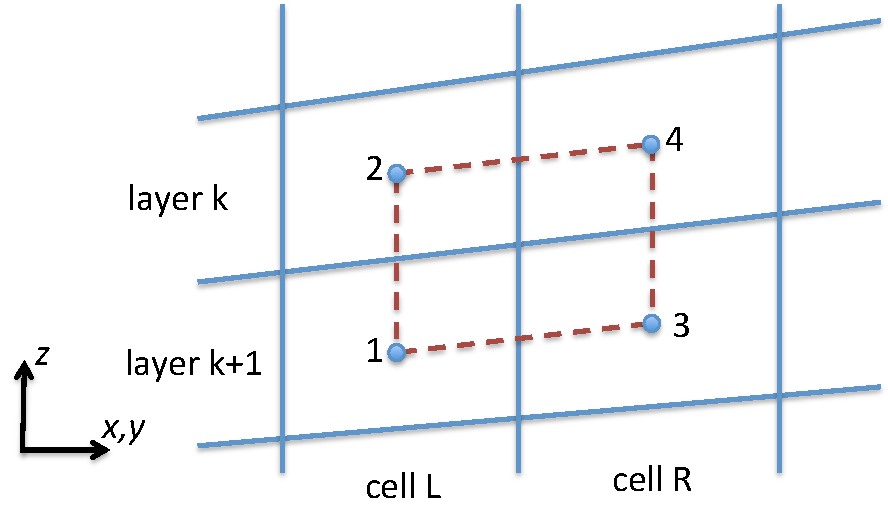
\includegraphics[width=3.5in]{ocean/figures/common_level.pdf}
\caption{Vertical cross-section of ocean grid cells, showing index locations for common level method.  The dots are placed at cell centers in the horizontal and layer mid-depth in the vertical.}
\label{oceanFigure:common level}
\end{figure}

{\bf \large config\_pressure\_gradient\_type = 'Jacobian\_from\_density'}\\
In this formulation the pressure gradient is rewritten in terms of a sea surface height gradient and the vertical integral of a Jacobian,
\begin{eqnarray}
\label{ocean:grad p Jacobian}
- \frac{1}{\rho_0}\nabla_z p &=& - \frac{\rho_s g}{\rho_0}\nabla_s \zeta - \frac{g}{\rho_0}\int_z^\zeta {\mathcal J}(\rho,z)ds, \\
{\mathcal J}(\rho,z) &=& \left. \frac{\partial \rho}{\partial x} \right|_s \frac{\partial z}{\partial s} 
 - \frac{\partial \rho}{\partial s}  \left. \frac{\partial z}{\partial x} \right|_s 
\end{eqnarray}
where $x$ is a general horizontal direction between two cell centers and $s$ is the vertical coordinate reference, i.e.\ $s$ is constant within a layer.  There are many methods to discretize the Jacobian term.  In the common level method, the density is linearly interpolated or extrapolated within each vertical column to a common level $z_\gamma$ (see Figure \ref{oceanFigure:common level}):
\begin{eqnarray}
- \int_z^\zeta {\mathcal J}(\rho,z)ds &=& \overline{\Delta z} \left( \rho^L - \rho^R \right) \\
\overline{\Delta z} &=& \frac{1}{2} \left(z_2-z_1 + z_4-z_3\right) \\
\rho^L &=& \frac{\rho_1\left(z_2-z_\gamma\right) + \rho_2\left(z_\gamma-z_1\right) }{z_2-z_1}\\
\rho^R &=& \frac{\rho_3\left(z_4-z_\gamma\right) + \rho_4\left(z_\gamma-z_3\right) }{z_4-z_3}\\
z_\gamma &=& \left(1-\gamma\right)z_* + \gamma z_c \\
z_* &=&  \frac{z_4 z_2-z_3z_1}{z_4-z_3 + z_2-z_1} \\
z_c &=&  \frac{z_1+z_2+z_3+z_4}{4} 
\end{eqnarray}
where $z_c$ is the depth for the weighted Jacobian method by \citet{Song98mwr}, and $z_*$ is the depth for the standard Jacobian method, which is the depth of intersection of the diagonals of the trapezoidal element in Figure \ref{oceanFigure:common level}.  Here $\gamma$ weights the choice between these two methods for computing the common level $z_\gamma$.  This formulation for the pressure gradient is described in detail in \citet{Shchepetkin_McWilliams03jgr}, Section 2, method 2, and Section 4.  They found that a coefficient of $\gamma=0.5$, which gives equal weights to the standard and weighted Jacobian methods, minimizes the errors in a seamount test problem.

{\bf \large config\_pressure\_gradient\_type = 'Jacobian\_from\_TS'}\\
This formulation is the same as the previous, except that the Jacobian is computed using a linear expansion in potential temperature and salinity.  This option must be used when layers are extremely tilted, such as with sigma coordinates or under an ice shelf, in combination with a nonlinear equation of state.
\begin{eqnarray}
 {\mathcal J}(\rho,z) &=& -\alpha  {\mathcal J}(\theta,z) + \beta  {\mathcal J}(S,z), 
\end{eqnarray}
where
\begin{eqnarray}
\alpha\left( \theta, S, p\right) &=&  -\left. \frac{\partial \rho}{\partial \theta} \right|_{S,p} \\
\beta\left( \theta, S, p\right) &=&  \left. \frac{\partial \rho}{\partial S} \right|_{\theta,p} 
\end{eqnarray}
are the thermal expansion and saline contraction coefficients, computed at a particular  $\left(\theta, S, p\right)$ by the equation of state \citep[eqn 7.16]{Shchepetkin_McWilliams03jgr}.

{\bf \large config\_pressure\_gradient\_type = 'MontgomeryPotential'}\\
For isopycnal vertical coordinates, the user may choose to use the Montgomery potential,
\begin{equation}
\label{ocean:Montgomery Potential}
M = \frac{1}{\rho}p+gz
\end{equation}
and replace the pressure terms above with
\begin{equation}
- \nabla_s M.
\end{equation}
See \citet[section 2.1]{Higdon05jcp} for details on the derivation and computation of the Montgomery potential.

% {\bf \large config\_pressure\_gradient\_type = 'MontgomeryPotential\_and\_density'}
% Same as previous, but this formulation includes an extra term,
% \begin{equation}
% - \nabla_s M + p \nabla_s\left(\frac{1}{\rho} \right),
% \end{equation}
% as described by \citet{Bleck02om}, eqn 1 and end of Appendix A.  This formulation has not been extensively tested and is not supported at this time.

\vspace{0.5in}
{\small
\begin{center}
\begin{longtable}{| p{2.0in} || p{4.0in} |}
	\hline
	{\bf Name} & {\bf Description} \endfirsthead
	\hline 
	{\bf Name} & {\bf Description} (Continued) \endhead
	\hline
	\hline
	\hyperref[sec:nm_sec_config_pressure_gradient_type]{config\_pressure\_gradient\_type} & Form of pressure gradient terms in momentum equation. For most applications, the gradient of pressure and layer mid-depth are appropriate.  For isopycnal coordinates, one may use the gradient of the Montgomery potential. \\
	\hline
	\hyperref[sec:nm_sec_config_density0]{config\_density0} &  Density used as a coefficient of the pressure gradient terms,  $\rho_0$ .  This is a constant due to the Boussinesq approximation. \\
	\hline
\end{longtable}
\end{center}
}
\subsection[eos]{eos}
\label{subsec:analysis_nm_tab_eos}
Two forms of EOS are supported. The full EOS from \cite{Jackett_McDougall95jaot} and a linear EOS.

\vspace{0.5in}
{\small
\begin{center}
\begin{longtable}{| p{2.0in} || p{4.0in} |}
	\hline
	{\bf Name} & {\bf Description} \endfirsthead
	\hline 
	{\bf Name} & {\bf Description} (Continued) \endhead
	\hline
	\hline
	\hyperref[sec:nm_sec_config_eos_type]{config\_eos\_type} & Character string to choose EOS formulation \\
	\hline
\end{longtable}
\end{center}
}
\subsection[eos\_linear]{eos\_linear}
\label{subsec:analysis_nm_tab_eos_linear}
The linear equation of state (leos) is specified as follows:
\begin{equation}
\rho = \rho_{ref} - \alpha_{leos}(T-T_{ref})+\beta_{leos}(S-S_{ref})
\end{equation}
\vspace{0.5in}
{\small
\begin{center}
\begin{longtable}{| p{2.0in} || p{4.0in} |}
	\hline
	{\bf Name} & {\bf Description} \endfirsthead
	\hline 
	{\bf Name} & {\bf Description} (Continued) \endhead
	\hline
	\hline
	\hyperref[sec:nm_sec_config_eos_linear_alpha]{config\_eos\_linear\_alpha} & Linear thermal expansion coefficient \\
	\hline
	\hyperref[sec:nm_sec_config_eos_linear_beta]{config\_eos\_linear\_beta} & Linear haline contraction coefficient \\
	\hline
	\hyperref[sec:nm_sec_config_eos_linear_Tref]{config\_eos\_linear\_Tref} & Reference temperature \\
	\hline
	\hyperref[sec:nm_sec_config_eos_linear_Sref]{config\_eos\_linear\_Sref} & Reference salinity \\
	\hline
	\hyperref[sec:nm_sec_config_eos_linear_densityref]{config\_eos\_linear\_densityref} & Reference density, i.e. density when T=Tref and S=Sref \\
	\hline
\end{longtable}
\end{center}
}
\subsection[split\_explicit\_ts]{split\_explicit\_ts}
\label{subsec:analysis_nm_tab_split_explicit_ts}
The split explicit time-stepping method solves the barotropic (vertically-integrated) velocities separately from the remaining baroclinic velocities.  The time step for the barotropic solve is limited by fast surface gravity waves, and so is subcycled within a large timestep of the baroclinic velocity solve.  This provides a 10 to 12-times speed-up over fourth-order Runge-Kutta time stepping.

A single large timestep in the split explicit algorithm may be summarized as
\begin{itemize}
\item Stage 1: solve for baroclinic velocity (3D)
\item Stage 2: solve for barotropic velocity (2D) with explicit sub-cycling
\item Stage 3: update thickness, tracers, density and pressure
\end{itemize}
The algorithm includes iterations within stage 1, within each subcycle of stage 2, and over the full three-stage process.  Further details are provided in \citet[Appendix A.5]{Ringler_ea13om}

\vspace{0.5in}
{\small
\begin{center}
\begin{longtable}{| p{2.0in} || p{4.0in} |}
	\hline
	{\bf Name} & {\bf Description} \endfirsthead
	\hline 
	{\bf Name} & {\bf Description} (Continued) \endhead
	\hline
	\hline
	\hyperref[sec:nm_sec_config_n_ts_iter]{config\_n\_ts\_iter} & number of large iterations over stages 1-3 \\
	\hline
	\hyperref[sec:nm_sec_config_n_bcl_iter_beg]{config\_n\_bcl\_iter\_beg} & number of iterations of stage 1 (baroclinic solve) on the first split-explicit iteration \\
	\hline
	\hyperref[sec:nm_sec_config_n_bcl_iter_mid]{config\_n\_bcl\_iter\_mid} & number of iterations of stage 1 (baroclinic solve) on any split-explicit iterations between first and last \\
	\hline
	\hyperref[sec:nm_sec_config_n_bcl_iter_end]{config\_n\_bcl\_iter\_end} & number of iterations of stage 1 (baroclinic solve) on the last split-explicit iteration \\
	\hline
	\hyperref[sec:nm_sec_config_n_btr_subcycles]{config\_n\_btr\_subcycles} & number of barotropic subcycles in stage 2 \\
	\hline
	\hyperref[sec:nm_sec_config_n_btr_cor_iter]{config\_n\_btr\_cor\_iter} & number of iterations of the velocity corrector step in stage 2 \\
	\hline
	\hyperref[sec:nm_sec_config_vel_correction]{config\_vel\_correction} & If true, the velocity correction term is included in the horizontal advection of thickness and tracers \\
	\hline
	\hyperref[sec:nm_sec_config_btr_subcycle_loop_factor]{config\_btr\_subcycle\_loop\_facto-}\hyperref[sec:nm_sec_config_btr_subcycle_loop_factor]{r}&  Barotropic subcycles proceed from  $t$  to  $t+n\Delta t$ , where  $n$  is this configuration option. \\
	\hline
	\hyperref[sec:nm_sec_config_btr_gam1_velWt1]{config\_btr\_gam1\_velWt1} & Weighting of velocity in the SSH predictor step in stage 2.  When zero, previous subcycle time is used; when one, new subcycle time is used. \\
	\hline
	\hyperref[sec:nm_sec_config_btr_gam2_SSHWt1]{config\_btr\_gam2\_SSHWt1} & Weighting of SSH in the velocity corrector step in stage 2.  When zero, previous subcycle time is used; when one, new subcycle time is used. \\
	\hline
	\hyperref[sec:nm_sec_config_btr_gam3_velWt2]{config\_btr\_gam3\_velWt2} & Weighting of velocity in the SSH corrector step in stage 2.  When zero, previous subcycle time is used; when one, new subcycle time is used. \\
	\hline
	\hyperref[sec:nm_sec_config_btr_solve_SSH2]{config\_btr\_solve\_SSH2} & If true, execute the SSH corrector step in stage 2 \\
	\hline
\end{longtable}
\end{center}
}
\subsection[testing]{testing}
\label{subsec:analysis_nm_tab_testing}
\section{Testing}
\label{sec:testing}

\vspace{0.5in}
{\small
\begin{center}
\begin{longtable}{| p{2.0in} || p{4.0in} |}
	\hline
	{\bf Name} & {\bf Description} \endfirsthead
	\hline 
	{\bf Name} & {\bf Description} (Continued) \endhead
	\hline
	\hline
	\hyperref[sec:nm_sec_config_conduct_tests]{config\_conduct\_tests} & If true, run testing suite.  This is the overarching control on the test suite.  Individual flags must be set to true below to conduct each test. \\
	\hline
	\hyperref[sec:nm_sec_config_test_tensors]{config\_test\_tensors} & If true, tensor operations are tested upon start-up. \\
	\hline
	\hyperref[sec:nm_sec_config_tensor_test_function]{config\_tensor\_test\_function} & Character string to choose tensor test fuction \\
	\hline
\end{longtable}
\end{center}
}
\subsection[debug]{debug}
\label{subsec:analysis_nm_tab_debug}
At run-time a user can enable debugging features within MPAS-Ocean. These
features include disabling any tendencies to help determine why an issue might
be happening. Debugging options also include various checks on certain fields,
and the ability to prescribe both a thickness and velocity field at run-time
which are constant throughout a simulation. All options that control these
debugging features are specified within the debug namelist record.

\vspace{0.5in}
{\small
\begin{center}
\begin{longtable}{| p{2.0in} || p{4.0in} |}
	\hline
	{\bf Name} & {\bf Description} \endfirsthead
	\hline 
	{\bf Name} & {\bf Description} (Continued) \endhead
	\hline
	\hline
	\hyperref[sec:nm_sec_config_check_zlevel_consistency]{config\_check\_zlevel\_consistency} & Enables a run-time check for consistency for a zlevel grid. Ensures relevant variables correctly define the bottom of the ocean. \\
	\hline
	\hyperref[sec:nm_sec_config_filter_btr_mode]{config\_filter\_btr\_mode} & Enables filtering of the barotropic mode. \\
	\hline
	\hyperref[sec:nm_sec_config_prescribe_velocity]{config\_prescribe\_velocity} & Enables a prescribed velocity field. This velocity field is read on input, and remains constant through a simulation. \\
	\hline
	\hyperref[sec:nm_sec_config_prescribe_thickness]{config\_prescribe\_thickness} & Enables a prescribed thickness field. This thickness field is read on input, and remains constant through a simulation. \\
	\hline
	\hyperref[sec:nm_sec_config_include_KE_vertex]{config\_include\_KE\_vertex} & If true, the kinetic energy in each cell is computed by blending cell-based and vertex-based values of kinetic energy. \\
	\hline
	\hyperref[sec:nm_sec_config_check_tracer_monotonicity]{config\_check\_tracer\_monotonici-}\hyperref[sec:nm_sec_config_check_tracer_monotonicity]{ty}& Enables a change on tracer monotonicity at the end of the monotonic advection routine. Only used if config\_monotonic is set to .true. \\
	\hline
	\hyperref[sec:nm_sec_config_disable_thick_all_tend]{config\_disable\_thick\_all\_tend} & Disables all tendencies on the thickness field. \\
	\hline
	\hyperref[sec:nm_sec_config_disable_thick_hadv]{config\_disable\_thick\_hadv} & Disable tendencies on the thickness field from horizontal advection. \\
	\hline
	\hyperref[sec:nm_sec_config_disable_thick_vadv]{config\_disable\_thick\_vadv} & Disables tendencies on the thickness field from vertical advection. \\
	\hline
	\hyperref[sec:nm_sec_config_disable_thick_sflux]{config\_disable\_thick\_sflux} & Disables tendencies on the thickness field from surface fluxes. \\
	\hline
	\hyperref[sec:nm_sec_config_disable_vel_all_tend]{config\_disable\_vel\_all\_tend} & Disables all tendencies on the velocity field. \\
	\hline
	\hyperref[sec:nm_sec_config_disable_vel_coriolis]{config\_disable\_vel\_coriolis} & Diables tendencies on the velocity field from the Coriolis force. \\
	\hline
	\hyperref[sec:nm_sec_config_disable_vel_pgrad]{config\_disable\_vel\_pgrad} & Disables tendencies on the velocity field from the horizontal pressure gradient. \\
	\hline
	\hyperref[sec:nm_sec_config_disable_vel_hmix]{config\_disable\_vel\_hmix} & Disables tendencies on the velocity field from horizontal mixing. \\
	\hline
	\hyperref[sec:nm_sec_config_disable_vel_windstress]{config\_disable\_vel\_windstress} & Disables tendencies on the velocity field from horizontal wind stress. \\
	\hline
	\hyperref[sec:nm_sec_config_disable_vel_vmix]{config\_disable\_vel\_vmix} & Disables tendencies on the velocity field from vertical mixing. \\
	\hline
	\hyperref[sec:nm_sec_config_disable_vel_vadv]{config\_disable\_vel\_vadv} & Disables tendencies on the velocity field from vertical advection. \\
	\hline
	\hyperref[sec:nm_sec_config_disable_tr_all_tend]{config\_disable\_tr\_all\_tend} & Disables all tendencies on tracer fields. \\
	\hline
	\hyperref[sec:nm_sec_config_disable_tr_adv]{config\_disable\_tr\_adv} & Disables tendencies on tracer fields from advection, both horizontal and vertical. \\
	\hline
	\hyperref[sec:nm_sec_config_disable_tr_hmix]{config\_disable\_tr\_hmix} & Disables tendencies on tracer fields from horizontal mixing. \\
	\hline
	\hyperref[sec:nm_sec_config_disable_tr_vmix]{config\_disable\_tr\_vmix} & Disables tendencies on tracer fields from vertical mixing. \\
	\hline
	\hyperref[sec:nm_sec_config_disable_tr_sflux]{config\_disable\_tr\_sflux} & Disables tendencies on tracer fields from surface fluxes. \\
	\hline
\end{longtable}
\end{center}
}
\subsection[ocn\_am\_global\_stats]{ocn\_am\_global\_stats}
\label{subsec:analysis_nm_tab_ocn_am_global_stats}
\vspace{0.5in}
{\small
\begin{center}
\begin{longtable}{| p{2.0in} || p{4.0in} |}
	\hline
	{\bf Name} & {\bf Description} \endfirsthead
	\hline 
	{\bf Name} & {\bf Description} (Continued) \endhead
	\hline
	\hline
	\hyperref[sec:nm_sec_config_ocn_am_global_stats]{config\_ocn\_am\_global\_stats} & If true, ocean analysis member global\_stats is called. \\
	\hline
\end{longtable}
\end{center}
}
\section[Variable definitions]{\hyperref[chap:variable_sections]{Variable definitions}}
\label{sec:analysis_variable_tables}
Embedded links point to more detailed variable information in the appendix.
\subsection[state]{\hyperref[sec:var_sec_state]{state}}
\label{subsec:analysis_var_tab_state}
The state data structure contains a set of prognostic and diagnostic fields
that are time dependent. The fields contained inside of state have two time
levels available in the default version of MPAS-Ocean.

\vspace{0.5in}
{\small
\begin{center}
\begin{longtable}{| p{2.0in} | p{4.0in} |}
	\hline
	{\bf Name} & {\bf Description} \endfirsthead
	\hline 
	{\bf Name} & {\bf Description} (Continued) \endhead
	\hline
	\hyperref[subsec:var_sec_state_temperature]{temperature} & potential temperature \\
	\hline
	\hyperref[subsec:var_sec_state_salinity]{salinity} & salinity \\
	\hline
	\hyperref[subsec:var_sec_state_tracer1]{tracer1} & tracer \\
	\hline
	\hyperref[subsec:var_sec_state_normalVelocity]{normalVelocity} & horizonal velocity, normal component to an edge \\
	\hline
	\hyperref[subsec:var_sec_state_layerThickness]{layerThickness} & layer thickness \\
	\hline
	\hyperref[subsec:var_sec_state_ssh]{ssh} & sea surface height \\
	\hline
	\hyperref[subsec:var_sec_state_highFreqThickness]{highFreqThickness} & high frequency-filtered layer thickness \\
	\hline
	\hyperref[subsec:var_sec_state_lowFreqDivergence]{lowFreqDivergence} & low frequency-filtered divergence \\
	\hline
	\hyperref[subsec:var_sec_state_normalBarotropicVelocity]{normalBarotropicVelocity} & barotropic velocity, used in split-explicit time-stepping \\
	\hline
	\hyperref[subsec:var_sec_state_normalBarotropicVelocitySubcycle]{normalBarotropicVelocitySubcy-}\hyperref[subsec:var_sec_state_normalBarotropicVelocitySubcycle]{cle  }& barotropic velocity, used in subcycling in stage 2 of split-explicit time-stepping \\
	\hline
	\hyperref[subsec:var_sec_state_sshSubcycle]{sshSubcycle} & sea surface height, used in subcycling in stage 2 of split-explicit time-stepping \\
	\hline
	\hyperref[subsec:var_sec_state_normalBaroclinicVelocity]{normalBaroclinicVelocity} & baroclinic velocity, used in split-explicit time-stepping \\
	\hline
\end{longtable}
\end{center}
}
\subsection[mesh]{\hyperref[sec:var_sec_mesh]{mesh}}
\label{subsec:analysis_var_tab_mesh}
The mesh data type contains a single time level. The fields inside the mesh
structure are not assumed to be time dependent. This data structure contains
fields that describe the mesh, and the connectivity of the mesh. Several of the
fields contained in this structure are shared throughout all MPAS dynamical
cores.

\vspace{0.5in}
{\small
\begin{center}
\begin{longtable}{| p{2.0in} | p{4.0in} |}
	\hline
	{\bf Name} & {\bf Description} \endfirsthead
	\hline 
	{\bf Name} & {\bf Description} (Continued) \endhead
	\hline
	\hyperref[subsec:var_sec_mesh_latCell]{latCell} & Latitude location of cell centers in radians. \\
	\hline
	\hyperref[subsec:var_sec_mesh_lonCell]{lonCell} & Longitude location of cell centers in radians. \\
	\hline
	\hyperref[subsec:var_sec_mesh_xCell]{xCell} & X Coordinate in cartesian space of cell centers. \\
	\hline
	\hyperref[subsec:var_sec_mesh_yCell]{yCell} & Y Coordinate in cartesian space of cell centers. \\
	\hline
	\hyperref[subsec:var_sec_mesh_zCell]{zCell} & Z Coordinate in cartesian space of cell centers. \\
	\hline
	\hyperref[subsec:var_sec_mesh_indexToCellID]{indexToCellID} & List of global cell IDs. \\
	\hline
	\hyperref[subsec:var_sec_mesh_latEdge]{latEdge} & Latitude location of edge midpoints in radians. \\
	\hline
	\hyperref[subsec:var_sec_mesh_lonEdge]{lonEdge} & Longitude location of edge midpoints in radians. \\
	\hline
	\hyperref[subsec:var_sec_mesh_xEdge]{xEdge} & X Coordinate in cartesian space of edge midpoints. \\
	\hline
	\hyperref[subsec:var_sec_mesh_yEdge]{yEdge} & Y Coordinate in cartesian space of edge midpoints. \\
	\hline
	\hyperref[subsec:var_sec_mesh_zEdge]{zEdge} & Z Coordinate in cartesian space of edge midpoints. \\
	\hline
	\hyperref[subsec:var_sec_mesh_indexToEdgeID]{indexToEdgeID} & List of global edge IDs. \\
	\hline
	\hyperref[subsec:var_sec_mesh_latVertex]{latVertex} & Latitude location of vertices in radians. \\
	\hline
	\hyperref[subsec:var_sec_mesh_lonVertex]{lonVertex} & Longitude location of vertices in radians. \\
	\hline
	\hyperref[subsec:var_sec_mesh_xVertex]{xVertex} & X Coordinate in cartesian space of vertices. \\
	\hline
	\hyperref[subsec:var_sec_mesh_yVertex]{yVertex} & Y Coordinate in cartesian space of vertices. \\
	\hline
	\hyperref[subsec:var_sec_mesh_zVertex]{zVertex} & Z Coordinate in cartesian space of vertices. \\
	\hline
	\hyperref[subsec:var_sec_mesh_indexToVertexID]{indexToVertexID} & List of global vertex IDs. \\
	\hline
	\hyperref[subsec:var_sec_mesh_meshDensity]{meshDensity} & Value of density function used to generate a particular mesh at cell centers. \\
	\hline
	\hyperref[subsec:var_sec_mesh_meshScalingDel2]{meshScalingDel2} & Coefficient to Laplacian mixing terms in momentum and tracer equations, so that viscosity and diffusion scale with mesh. \\
	\hline
	\hyperref[subsec:var_sec_mesh_meshScalingDel4]{meshScalingDel4} & Coefficient to biharmonic mixing terms in momentum and tracer equations, so that biharmonic viscosity and diffusion coefficients scale with mesh. \\
	\hline
	\hyperref[subsec:var_sec_mesh_meshScaling]{meshScaling} & Coefficient used for mesh scaling, such as the Leith parameter. \\
	\hline
	\hyperref[subsec:var_sec_mesh_cellsOnEdge]{cellsOnEdge} & List of cells that straddle each edge. \\
	\hline
	\hyperref[subsec:var_sec_mesh_nEdgesOnCell]{nEdgesOnCell} & Number of edges that border each cell. \\
	\hline
	\hyperref[subsec:var_sec_mesh_nEdgesOnEdge]{nEdgesOnEdge} & Number of edges that surround each of the cells that straddle each edge. These edges are used to reconstruct the tangential velocities. \\
	\hline
	\hyperref[subsec:var_sec_mesh_edgesOnCell]{edgesOnCell} & List of edges that border each cell. \\
	\hline
	\hyperref[subsec:var_sec_mesh_edgesOnEdge]{edgesOnEdge} & List of edges that border each of the cells that straddle each edge. \\
	\hline
	\hyperref[subsec:var_sec_mesh_weightsOnEdge]{weightsOnEdge} & Reconstruction weights associated with each of the edgesOnEdge. \\
	\hline
	\hyperref[subsec:var_sec_mesh_dvEdge]{dvEdge} & Length of each edge, computed as the distance between verticesOnEdge. \\
	\hline
	\hyperref[subsec:var_sec_mesh_dcEdge]{dcEdge} & Length of each edge, computed as the distance between cellsOnEdge. \\
	\hline
	\hyperref[subsec:var_sec_mesh_angleEdge]{angleEdge} & Angle the edge normal makes with local eastward direction. \\
	\hline
	\hyperref[subsec:var_sec_mesh_areaCell]{areaCell} & Area of each cell in the primary grid. \\
	\hline
	\hyperref[subsec:var_sec_mesh_areaTriangle]{areaTriangle} & Area of each cell (triangle) in the dual grid. \\
	\hline
	\hyperref[subsec:var_sec_mesh_edgeNormalVectors]{edgeNormalVectors} & Normal unit vector defined at an edge. \\
	\hline
	\hyperref[subsec:var_sec_mesh_edgeTangentVectors]{edgeTangentVectors} & Tangent unit vector defined at an edge. \\
	\hline
	\hyperref[subsec:var_sec_mesh_localVerticalUnitVectors]{localVerticalUnitVectors} & Unit surface normal vectors defined at cell centers. \\
	\hline
	\hyperref[subsec:var_sec_mesh_cellTangentPlane]{cellTangentPlane} & The two vectors that define a tangent plane at a cell center. \\
	\hline
	\hyperref[subsec:var_sec_mesh_cellsOnCell]{cellsOnCell} & List of cells that neighbor each cell. \\
	\hline
	\hyperref[subsec:var_sec_mesh_verticesOnCell]{verticesOnCell} & List of vertices that border each cell. \\
	\hline
	\hyperref[subsec:var_sec_mesh_verticesOnEdge]{verticesOnEdge} & List of vertices that straddle each edge. \\
	\hline
	\hyperref[subsec:var_sec_mesh_edgesOnVertex]{edgesOnVertex} & List of edges that share a vertex as an endpoint. \\
	\hline
	\hyperref[subsec:var_sec_mesh_cellsOnVertex]{cellsOnVertex} & List of cells that share a vertex. \\
	\hline
	\hyperref[subsec:var_sec_mesh_kiteAreasOnVertex]{kiteAreasOnVertex} & Area of the portions of each dual cell that are part of each cellsOnVertex. \\
	\hline
	\hyperref[subsec:var_sec_mesh_fEdge]{fEdge} & Coriolis parameter at edges. \\
	\hline
	\hyperref[subsec:var_sec_mesh_fVertex]{fVertex} & Coriolis parameter at vertices. \\
	\hline
	\hyperref[subsec:var_sec_mesh_fCell]{fCell} & Coriolis parameter at cell centers. \\
	\hline
	\hyperref[subsec:var_sec_mesh_bottomDepth]{bottomDepth} & Depth of the bottom of the ocean. Given as a positive distance from sea level. \\
	\hline
	\hyperref[subsec:var_sec_mesh_derivTwo]{derivTwo} & Value of the second derivative of the polynomial used for reconstruction of cell center quantities at edges. \\
	\hline
	\hyperref[subsec:var_sec_mesh_advCoefs]{advCoefs} & Weighting coefficients used for reconstruction of cell center quantities at edges. Used in advection routines. \\
	\hline
	\hyperref[subsec:var_sec_mesh_advCoefs3rd]{advCoefs3rd} & Wegihting coefficients used for reconstruction of cell center quantities at edges. Used in advection routines. \\
	\hline
	\hyperref[subsec:var_sec_mesh_advCellsForEdge]{advCellsForEdge} & List of cells used to reconstruct a cell quantity at an edge. Used in advection routines. \\
	\hline
	\hyperref[subsec:var_sec_mesh_nAdvCellsForEdge]{nAdvCellsForEdge} & Number of cells used in reconstruction of cell center quantities at an edge. Used in advection routines. \\
	\hline
	\hyperref[subsec:var_sec_mesh_highOrderAdvectionMask]{highOrderAdvectionMask} & Mask for high order advection. Values are 1 if high order is used, and 0 if not. \\
	\hline
	\hyperref[subsec:var_sec_mesh_coeffs_reconstruct]{coeffs\_reconstruct} & Coefficients to reconstruct velocity vectors at cells centers. \\
	\hline
	\hyperref[subsec:var_sec_mesh_maxLevelCell]{maxLevelCell} & Index to the last active ocean cell in each column. \\
	\hline
	\hyperref[subsec:var_sec_mesh_maxLevelEdgeTop]{maxLevelEdgeTop} & Index to the last edge in a column with active ocean cells on both sides of it. \\
	\hline
	\hyperref[subsec:var_sec_mesh_maxLevelEdgeBot]{maxLevelEdgeBot} & Index to the last edge in a column with at least one active ocean cell on either side of it. \\
	\hline
	\hyperref[subsec:var_sec_mesh_maxLevelVertexTop]{maxLevelVertexTop} & Index to the last vertex in a column with all active cells around it. \\
	\hline
	\hyperref[subsec:var_sec_mesh_maxLevelVertexBot]{maxLevelVertexBot} & Index to the last vertex in a column with at least one active ocean cell around it. \\
	\hline
	\hyperref[subsec:var_sec_mesh_refBottomDepth]{refBottomDepth} & Reference depth of ocean for each vertical level. Used in 'z-level' type runs. \\
	\hline
	\hyperref[subsec:var_sec_mesh_refBottomDepthTopOfCell]{refBottomDepthTopOfCell} & Reference depth of ocean for each vertical interface. Used in 'z-level' type runs. \\
	\hline
	\hyperref[subsec:var_sec_mesh_vertCoordMovementWeights]{vertCoordMovementWeights} & Weights used for distribution of sea surface heigh purturbations through multiple vertical levels. \\
	\hline
	\hyperref[subsec:var_sec_mesh_boundaryEdge]{boundaryEdge} & Mask for determining boundary edges. A boundary edge has only one active ocean cell neighboring it. \\
	\hline
	\hyperref[subsec:var_sec_mesh_boundaryVertex]{boundaryVertex} & Mask for determining boundary vertices. A boundary vertex has at least one inactive cell neighboring it. \\
	\hline
	\hyperref[subsec:var_sec_mesh_boundaryCell]{boundaryCell} & Mask for determining boundary cells. A boundary cell has at least one inactive cell neighboring it. \\
	\hline
	\hyperref[subsec:var_sec_mesh_edgeMask]{edgeMask} & Mask on edges that determines if computations should be done on edge. \\
	\hline
	\hyperref[subsec:var_sec_mesh_vertexMask]{vertexMask} & Mask on vertices that determines if computations should be done on vertice. \\
	\hline
	\hyperref[subsec:var_sec_mesh_cellMask]{cellMask} & Mask on cells that determines if computations should be done on cell. \\
	\hline
	\hyperref[subsec:var_sec_mesh_temperatureRestore]{temperatureRestore} & Temperature restoring field, for restoring temperature at the surface. \\
	\hline
	\hyperref[subsec:var_sec_mesh_salinityRestore]{salinityRestore} & Salinity restoring field, for restoring salinity at the surface. \\
	\hline
	\hyperref[subsec:var_sec_mesh_edgeSignOnCell]{edgeSignOnCell} & Sign of edge contributions to a cell for each edge on cell. Used for bit-reproducible loops. Represents directionality of vector connecting cells. \\
	\hline
	\hyperref[subsec:var_sec_mesh_edgeSignOnVertex]{edgeSignOnVertex} & Sign of edge contributions to a vertex for each edge on vertex. Used for bit-reproducible loops. Represents directionality of vector connecting vertices. \\
	\hline
	\hyperref[subsec:var_sec_mesh_kiteIndexOnCell]{kiteIndexOnCell} & Index of kite in dual grid, based on verticesOnCell. \\
	\hline
\end{longtable}
\end{center}
}
\subsection[verticalMesh]{\hyperref[sec:var_sec_verticalMesh]{verticalMesh}}
\label{subsec:analysis_var_tab_verticalMesh}
The vertical mesh data type contains a single time level. The fields inside the
vertical mesh structure are not assumed to be time dependent. This data
structure contains fields that describe the vertical mesh and are used for
various types of vertical meshes.

\vspace{0.5in}
{\small
\begin{center}
\begin{longtable}{| p{2.0in} | p{4.0in} |}
	\hline
	{\bf Name} & {\bf Description} \endfirsthead
	\hline 
	{\bf Name} & {\bf Description} (Continued) \endhead
	\hline
	\hyperref[subsec:var_sec_verticalMesh_restingThickness]{restingThickness} & Layer thickness when the ocean is at rest, i.e. without SSH or internal perturbations. \\
	\hline
	\hyperref[subsec:var_sec_verticalMesh_refZMid]{refZMid} & Reference mid z-coordinate of ocean for each vertical level.  This has a negative value. \\
	\hline
	\hyperref[subsec:var_sec_verticalMesh_refLayerThickness]{refLayerThickness} & Reference layerThickness of ocean for each vertical level. \\
	\hline
\end{longtable}
\end{center}
}
\subsection[tend]{\hyperref[sec:var_sec_tend]{tend}}
\label{subsec:analysis_var_tab_tend}
The tend data structure represents the tendencies used to time step the
prognostic variables within the state structure. 

\vspace{0.5in}
{\small
\begin{center}
\begin{longtable}{| p{2.0in} | p{4.0in} |}
	\hline
	{\bf Name} & {\bf Description} \endfirsthead
	\hline 
	{\bf Name} & {\bf Description} (Continued) \endhead
	\hline
	\hyperref[subsec:var_sec_tend_tendTemperature]{tendTemperature} & time tendency of potential temperature \\
	\hline
	\hyperref[subsec:var_sec_tend_tendSalinity]{tendSalinity} & time tendency of salinity measured as change in practical salinity units per second \\
	\hline
	\hyperref[subsec:var_sec_tend_tendTracer1]{tendTracer1} & test tracer \\
	\hline
	\hyperref[subsec:var_sec_tend_tendNormalVelocity]{tendNormalVelocity} & time tendency of normal component of velocity \\
	\hline
	\hyperref[subsec:var_sec_tend_tendLayerThickness]{tendLayerThickness} & time tendency of layer thickness \\
	\hline
	\hyperref[subsec:var_sec_tend_tendSsh]{tendSsh} & time tendency of sea-surface height \\
	\hline
	\hyperref[subsec:var_sec_tend_tendHighFreqThickness]{tendHighFreqThickness} & time tendency of high frequency-filtered layer thickness \\
	\hline
	\hyperref[subsec:var_sec_tend_tendLowFreqDivergence]{tendLowFreqDivergence} & time tendency of low frequency-filtered divergence \\
	\hline
\end{longtable}
\end{center}
}
\subsection[diagnostics]{\hyperref[sec:var_sec_diagnostics]{diagnostics}}
\label{subsec:analysis_var_tab_diagnostics}
The diagnostics type contains a set of diagnostics variables that are only
generally used in specific parts of MPAS-Ocean.

\vspace{0.5in}
{\small
\begin{center}
\begin{longtable}{| p{2.0in} | p{4.0in} |}
	\hline
	{\bf Name} & {\bf Description} \endfirsthead
	\hline 
	{\bf Name} & {\bf Description} (Continued) \endhead
	\hline
	\hyperref[subsec:var_sec_diagnostics_xtime]{xtime} & model time, with format 'YYYY-MM-DD\_HH:MM:SS' \\
	\hline
	\hyperref[subsec:var_sec_diagnostics_temperatureSurfaceValue]{temperatureSurfaceValue} & potential temperature extrapolated to ocean surface \\
	\hline
	\hyperref[subsec:var_sec_diagnostics_salinitySurfaceValue]{salinitySurfaceValue} & salinity extrapolated to ocean surface \\
	\hline
	\hyperref[subsec:var_sec_diagnostics_tracer1SurfaceValue]{tracer1SurfaceValue} & Tracer of 1 extrapolated to ocean surface \\
	\hline
	\hyperref[subsec:var_sec_diagnostics_zonalSurfaceVelocity]{zonalSurfaceVelocity} & Zonal surface velocity reconstructed at cell centers \\
	\hline
	\hyperref[subsec:var_sec_diagnostics_meridionalSurfaceVelocity]{meridionalSurfaceVelocity} & Meridional surface velocity reconstructed at cell centers \\
	\hline
	\hyperref[subsec:var_sec_diagnostics_zonalSSHGradient]{zonalSSHGradient} & Zonal gradient of SSH reconstructed at cell centers \\
	\hline
	\hyperref[subsec:var_sec_diagnostics_meridionalSSHGradient]{meridionalSSHGradient} & Meridional gradient of SSH reconstructed at cell centers \\
	\hline
	\hyperref[subsec:var_sec_diagnostics_zMid]{zMid} & z-coordinate of the mid-depth of the layer \\
	\hline
	\hyperref[subsec:var_sec_diagnostics_zTop]{zTop} & z-coordinate of the top of the layer \\
	\hline
	\hyperref[subsec:var_sec_diagnostics_density]{density} & density \\
	\hline
	\hyperref[subsec:var_sec_diagnostics_displacedDensity]{displacedDensity} & Density displaced adiabatically to the mid-depth one layer deeper.  That is, layer k has been displaced to the depth of layer k+1. \\
	\hline
	\hyperref[subsec:var_sec_diagnostics_potentialDensity]{potentialDensity} & potential density: density displaced adiabatically to the mid-depth of top layer \\
	\hline
	\hyperref[subsec:var_sec_diagnostics_BruntVaisalaFreqTop]{BruntVaisalaFreqTop} & Brunt Vaisala frequency defined at the center (horizontally) and top (vertically) of cell \\
	\hline
	\hyperref[subsec:var_sec_diagnostics_montgomeryPotential]{montgomeryPotential} & Montgomery potential, may be used as the pressure for isopycnal coordinates. \\
	\hline
	\hyperref[subsec:var_sec_diagnostics_pressure]{pressure} & pressure used in the momentum equation \\
	\hline
	\hyperref[subsec:var_sec_diagnostics_uTransport]{uTransport} & horizontal velocity used to transport mass and tracers \\
	\hline
	\hyperref[subsec:var_sec_diagnostics_vertTransportVelocityTop]{vertTransportVelocityTop} & vertical transport through the layer interface at the top of the cell \\
	\hline
	\hyperref[subsec:var_sec_diagnostics_vertVelocityTop]{vertVelocityTop} & vertical velocity defined at center (horizonally) and top (vertically) of cell \\
	\hline
	\hyperref[subsec:var_sec_diagnostics_tangentialVelocity]{tangentialVelocity} & horizontal velocity, tangential to an edge \\
	\hline
	\hyperref[subsec:var_sec_diagnostics_layerThicknessEdge]{layerThicknessEdge} & layer thickness averaged from cell center to edges \\
	\hline
	\hyperref[subsec:var_sec_diagnostics_layerThicknessVertex]{layerThicknessVertex} & layer thickness averaged from cell center to vertices \\
	\hline
	\hyperref[subsec:var_sec_diagnostics_kineticEnergyCell]{kineticEnergyCell} & kinetic energy of horizonal velocity on cells \\
	\hline
	\hyperref[subsec:var_sec_diagnostics_hEddyFlux]{hEddyFlux} & Eddy flux in Gent-McWilliams eddy parameterization \\
	\hline
	\hyperref[subsec:var_sec_diagnostics_hKappa]{hKappa} & kappa parameter for Gent-McWilliams eddy parameterization \\
	\hline
	\hyperref[subsec:var_sec_diagnostics_hKappaQ]{hKappaQ} & kappaQ parameter for Gent-McWilliams eddy parameterization \\
	\hline
	\hyperref[subsec:var_sec_diagnostics_viscosity]{viscosity} & horizontal viscosity \\
	\hline
	\hyperref[subsec:var_sec_diagnostics_divergence]{divergence} & divergence of horizonal velocity \\
	\hline
	\hyperref[subsec:var_sec_diagnostics_circulation]{circulation} & area-integrated vorticity \\
	\hline
	\hyperref[subsec:var_sec_diagnostics_relativeVorticity]{relativeVorticity} & curl of horizontal velocity, defined at vertices \\
	\hline
	\hyperref[subsec:var_sec_diagnostics_relativeVorticityCell]{relativeVorticityCell} & curl of horizontal velocity, averaged from vertices to cell centers \\
	\hline
	\hyperref[subsec:var_sec_diagnostics_normalizedRelativeVorticityEdge]{normalizedRelativeVorticityEdge} & curl of horizontal velocity divided by layer thickness, averaged from vertices to edges \\
	\hline
	\hyperref[subsec:var_sec_diagnostics_normalizedPlanetaryVorticityEdge]{normalizedPlanetaryVorticityEd-}\hyperref[subsec:var_sec_diagnostics_normalizedPlanetaryVorticityEdge]{ge  }& earth's rotational rate (Coriolis parameter, f) divided by layer thickness, averaged from vertices to edges \\
	\hline
	\hyperref[subsec:var_sec_diagnostics_normalizedRelativeVorticityCell]{normalizedRelativeVorticityCell} & curl of horizontal velocity divided by layer thickness, averaged from vertices to cell centers \\
	\hline
	\hyperref[subsec:var_sec_diagnostics_barotropicForcing]{barotropicForcing} & Barotropic tendency computed from the baroclinic equations in stage 1 of the split-explicit algorithm. \\
	\hline
	\hyperref[subsec:var_sec_diagnostics_barotropicThicknessFlux]{barotropicThicknessFlux} & Barotropic thickness flux at each edge, used to advance sea surface height in each subcycle of stage 2 of the split-explicit algorithm. \\
	\hline
	\hyperref[subsec:var_sec_diagnostics_normalVelocityX]{normalVelocityX} & component of horizontal velocity in the x-direction (cartesian) \\
	\hline
	\hyperref[subsec:var_sec_diagnostics_normalVelocityY]{normalVelocityY} & component of horizontal velocity in the y-direction (cartesian) \\
	\hline
	\hyperref[subsec:var_sec_diagnostics_normalVelocityZ]{normalVelocityZ} & component of horizontal velocity in the z-direction (cartesian) \\
	\hline
	\hyperref[subsec:var_sec_diagnostics_normalVelocityZonal]{normalVelocityZonal} & component of horizontal velocity in the eastward direction \\
	\hline
	\hyperref[subsec:var_sec_diagnostics_normalVelocityMeridional]{normalVelocityMeridional} & component of horizontal velocity in the northward \\
	\hline
	\hyperref[subsec:var_sec_diagnostics_gradSSH]{gradSSH} & Gradient of sea surface height at edges. \\
	\hline
	\hyperref[subsec:var_sec_diagnostics_gradSSHX]{gradSSHX} & X Component of the gradient of sea surface height at cell centers. \\
	\hline
	\hyperref[subsec:var_sec_diagnostics_gradSSHY]{gradSSHY} & Y Component of the gradient of sea surface height at cell centers. \\
	\hline
	\hyperref[subsec:var_sec_diagnostics_gradSSHZ]{gradSSHZ} & Z Component of the gradient of sea surface height at cell centers. \\
	\hline
	\hyperref[subsec:var_sec_diagnostics_gradSSHZonal]{gradSSHZonal} & Zonal Component of the gradient of sea surface height at cell centers. \\
	\hline
	\hyperref[subsec:var_sec_diagnostics_gradSSHMeridional]{gradSSHMeridional} & Meridional Component of the gradient of sea surface height at cell centers. \\
	\hline
	\hyperref[subsec:var_sec_diagnostics_uBolusGM]{uBolusGM} & Bolus velocity in Gent-McWilliams eddy parameterization \\
	\hline
	\hyperref[subsec:var_sec_diagnostics_uBolusGMX]{uBolusGMX} & Bolus velocity in Gent-McWilliams eddy parameterization, x-direction \\
	\hline
	\hyperref[subsec:var_sec_diagnostics_uBolusGMY]{uBolusGMY} & Bolus velocity in Gent-McWilliams eddy parameterization, y-direction \\
	\hline
	\hyperref[subsec:var_sec_diagnostics_uBolusGMZ]{uBolusGMZ} & Bolus velocity in Gent-McWilliams eddy parameterization, z-direction \\
	\hline
	\hyperref[subsec:var_sec_diagnostics_uBolusGMZonal]{uBolusGMZonal} & Bolus velocity in Gent-McWilliams eddy parameterization, zonal-direction \\
	\hline
	\hyperref[subsec:var_sec_diagnostics_uBolusGMMeridional]{uBolusGMMeridional} & Bolus velocity in Gent-McWilliams eddy parameterization, meridional-direction \\
	\hline
	\hyperref[subsec:var_sec_diagnostics_RiTopOfCell]{RiTopOfCell} & gradient Richardson number defined at the center (horizontally) and top (vertically) \\
	\hline
	\hyperref[subsec:var_sec_diagnostics_RiTopOfEdge]{RiTopOfEdge} & gradient Richardson number defined at the edge (horizontally) and top (vertically) \\
	\hline
	\hyperref[subsec:var_sec_diagnostics_vertViscTopOfEdge]{vertViscTopOfEdge} & vertical viscosity defined at the edge (horizontally) and top (vertically) \\
	\hline
	\hyperref[subsec:var_sec_diagnostics_vertViscTopOfCell]{vertViscTopOfCell} & vertical viscosity defined at the cell center (horizontally) and top (vertically) \\
	\hline
	\hyperref[subsec:var_sec_diagnostics_vertDiffTopOfCell]{vertDiffTopOfCell} & vertical diffusion defined at the cell center (horizontally) and top (vertically) \\
	\hline
	\hyperref[subsec:var_sec_diagnostics_bulkRichardsonNumber]{bulkRichardsonNumber} & bulk Richardson number \\
	\hline
	\hyperref[subsec:var_sec_diagnostics_boundaryLayerDepth]{boundaryLayerDepth} & diagnosed depth of the ocean surface boundary layer \\
	\hline
	\hyperref[subsec:var_sec_diagnostics_indexBoundaryLayerDepth]{indexBoundaryLayerDepth} & int(indexBoundaryLayerDepth) is vertical layer within which boundaryLayerDepth resides. mod(indexBoundaryLayerDepth) is fractional position within that layer. \\
	\hline
	\hyperref[subsec:var_sec_diagnostics_surfaceFrictionVelocity]{surfaceFrictionVelocity} & diagnosed surface friction velocity defined as square root of (mag(wind stress) / reference density) \\
	\hline
	\hyperref[subsec:var_sec_diagnostics_windStressZonalDiag]{windStressZonalDiag} & reconstructed surface wind stress in the eastward direction. Used for diagnostics. \\
	\hline
	\hyperref[subsec:var_sec_diagnostics_windStressMeridionalDiag]{windStressMeridionalDiag} & reconstructed surface wind stress in the northward direction. User for diagnostics. \\
	\hline
	\hyperref[subsec:var_sec_diagnostics_penetrativeTemperatureFluxOBL]{penetrativeTemperatureFluxO-}\hyperref[subsec:var_sec_diagnostics_penetrativeTemperatureFluxOBL]{BL  }& Penetrative temperature flux at the bottom of boundary layer due to solar radiation. Positive is into the ocean. \\
	\hline
	\hyperref[subsec:var_sec_diagnostics_buoyancyForcingOBL]{buoyancyForcingOBL} & diagnosed buoyancy forcing due to heat, salt and freshwater fluxes averaged over ocean boundary layer depth \\
	\hline
	\hyperref[subsec:var_sec_diagnostics_areaCellGlobal]{areaCellGlobal} & sum of the areaCell variable over the full domain, used to normalize global statistics \\
	\hline
	\hyperref[subsec:var_sec_diagnostics_areaEdgeGlobal]{areaEdgeGlobal} & sum of the areaEdge variable over the full domain, used to normalize global statistics \\
	\hline
	\hyperref[subsec:var_sec_diagnostics_areaTriangleGlobal]{areaTriangleGlobal} & sum of the areaTriangle variable over the full domain, used to normalize global statistics \\
	\hline
	\hyperref[subsec:var_sec_diagnostics_volumeCellGlobal]{volumeCellGlobal} & sum of the volumeCell variable over the full domain, used to normalize global statistics \\
	\hline
	\hyperref[subsec:var_sec_diagnostics_volumeEdgeGlobal]{volumeEdgeGlobal} & sum of the volumeEdge variable over the full domain, used to normalize global statistics \\
	\hline
	\hyperref[subsec:var_sec_diagnostics_CFLNumberGlobal]{CFLNumberGlobal} & maximum CFL number over the full domain \\
	\hline
\end{longtable}
\end{center}
}
\subsection[average]{\hyperref[sec:var_sec_average]{average}}
\label{subsec:analysis_var_tab_average}
The average data type contains a single time level. The fields inside the
average structure are not assumed to be time dependent. This data structure
contains fields that are time averages of other fields.

\vspace{0.5in}
{\small
\begin{center}
\begin{longtable}{| p{2.0in} | p{4.0in} |}
	\hline
	{\bf Name} & {\bf Description} \endfirsthead
	\hline 
	{\bf Name} & {\bf Description} (Continued) \endhead
	\hline
	\hyperref[subsec:var_sec_average_nAverage]{nAverage} & number of timesteps in time-averaged variables \\
	\hline
	\hyperref[subsec:var_sec_average_avgSsh]{avgSsh} & time-averaged sea surface height \\
	\hline
	\hyperref[subsec:var_sec_average_varSsh]{varSsh} & variance of sea surface height \\
	\hline
	\hyperref[subsec:var_sec_average_avgVelocityZonal]{avgVelocityZonal} & time-averaged velocity in the eastward direction \\
	\hline
	\hyperref[subsec:var_sec_average_avgVelocityMeridional]{avgVelocityMeridional} & time-averaged velocity in the northward direction \\
	\hline
	\hyperref[subsec:var_sec_average_varVelocityZonal]{varVelocityZonal} & variance of velocity in the eastward direction \\
	\hline
	\hyperref[subsec:var_sec_average_varVelocityMeridional]{varVelocityMeridional} & variance of velocity in the northward direction \\
	\hline
	\hyperref[subsec:var_sec_average_avgNormalVelocity]{avgNormalVelocity} & time-averaged velocity, normal to cell edge \\
	\hline
	\hyperref[subsec:var_sec_average_varNormalVelocity]{varNormalVelocity} & variance of velocity, normal to cell edge \\
	\hline
	\hyperref[subsec:var_sec_average_avgVertVelocityTop]{avgVertVelocityTop} & time-averaged vertical velocity at top of cell \\
	\hline
\end{longtable}
\end{center}
}
\subsection[forcing]{\hyperref[sec:var_sec_forcing]{forcing}}
\label{subsec:analysis_var_tab_forcing}
The forcing data type contains a single time level. The forcing structure
contains fields related to surface fluxes, wind stress, and fields that can be
used to compute surface fluxes.

\vspace{0.5in}
{\small
\begin{center}
\begin{longtable}{| p{2.0in} | p{4.0in} |}
	\hline
	{\bf Name} & {\bf Description} \endfirsthead
	\hline 
	{\bf Name} & {\bf Description} (Continued) \endhead
	\hline
	\hyperref[subsec:var_sec_forcing_surfaceWindStress]{surfaceWindStress} & Wind stress at the surface of the ocean defined at edge midpoints. Magintude in direction of edge normal. \\
	\hline
	\hyperref[subsec:var_sec_forcing_surfaceWindStressMagnitude]{surfaceWindStressMagnitude} & Magnitude of wind stress at the surface of the ocean, at cell centers. \\
	\hline
	\hyperref[subsec:var_sec_forcing_surfaceMassFlux]{surfaceMassFlux} & Flux of mass through the ocean surface. Positive into ocean. \\
	\hline
	\hyperref[subsec:var_sec_forcing_surfaceTemperatureFlux]{surfaceTemperatureFlux} & Flux of temperature through the ocean surface. Positive into ocean. \\
	\hline
	\hyperref[subsec:var_sec_forcing_surfaceSalinityFlux]{surfaceSalinityFlux} & Flux of salinity through the ocean surface. Positive into ocean. \\
	\hline
	\hyperref[subsec:var_sec_forcing_surfaceTracer1Flux]{surfaceTracer1Flux} & Flux of tracer1 through the ocean surface. Positive into ocean. \\
	\hline
	\hyperref[subsec:var_sec_forcing_seaSurfacePressure]{seaSurfacePressure} & Pressure defined at the sea surface. \\
	\hline
	\hyperref[subsec:var_sec_forcing_seaIceEnergy]{seaIceEnergy} &  Energy per unit area trapped in frazil ice formation. Always  $\ge$  0.0. \\
	\hline
	\hyperref[subsec:var_sec_forcing_penetrativeTemperatureFlux]{penetrativeTemperatureFlux} & Penetrative temperature flux at the surface due to solar radiation. Positive is into the ocean. \\
	\hline
	\hyperref[subsec:var_sec_forcing_transmissionCoefficients]{transmissionCoefficients} & Divergence of transmission through interfaces of surface fluxes below the surface layer at cell centers. These are not applied to short wave. \\
	\hline
	\hyperref[subsec:var_sec_forcing_windStressZonal]{windStressZonal} & Zonal (eastward) component of wind stress at cell centers from coupler. Positive eastward. \\
	\hline
	\hyperref[subsec:var_sec_forcing_windStressMeridional]{windStressMeridional} & Meridional (northward) component of wind stress at cell centers from coupler. Positive northward. \\
	\hline
	\hyperref[subsec:var_sec_forcing_latentHeatFlux]{latentHeatFlux} & Latent heat flux at cell centers from coupler. Positive into the ocean. \\
	\hline
	\hyperref[subsec:var_sec_forcing_sensibleHeatFlux]{sensibleHeatFlux} & Sensible heat flux at cell centers from coupler. Positive into the ocean. \\
	\hline
	\hyperref[subsec:var_sec_forcing_longWaveHeatFluxUp]{longWaveHeatFluxUp} & Upward long wave heat flux at cell centers from coupler. Positive into the ocean. \\
	\hline
	\hyperref[subsec:var_sec_forcing_longWaveHeatFluxDown]{longWaveHeatFluxDown} & Downward long wave heat flux at cell centers from coupler. Positive into the ocean. \\
	\hline
	\hyperref[subsec:var_sec_forcing_seaIceHeatFlux]{seaIceHeatFlux} & Sea ice heat flux at cell centers from coupler. Positive into the ocean. \\
	\hline
	\hyperref[subsec:var_sec_forcing_shortWaveHeatFlux]{shortWaveHeatFlux} & Short wave flux at cell centers from coupler. Positive into the ocean. \\
	\hline
	\hyperref[subsec:var_sec_forcing_evaporationFlux]{evaporationFlux} & Evaporation flux at cell centers from coupler. Positive into the ocean. \\
	\hline
	\hyperref[subsec:var_sec_forcing_seaIceSalinityFlux]{seaIceSalinityFlux} & Sea ice salinity flux at cell centers from coupler. Positive into the ocean. \\
	\hline
	\hyperref[subsec:var_sec_forcing_seaIceFreshWaterFlux]{seaIceFreshWaterFlux} & Fresh water flux from sea ice at cell centers from coupler. Positive into the ocean. \\
	\hline
	\hyperref[subsec:var_sec_forcing_riverRunoffFlux]{riverRunoffFlux} & Fresh water flux from river runoff at cell centers from coupler. Positive into the ocean. \\
	\hline
	\hyperref[subsec:var_sec_forcing_iceRunoffFlux]{iceRunoffFlux} & Fresh water flux from ice runoff at cell centers from coupler. Positive into the ocean. \\
	\hline
	\hyperref[subsec:var_sec_forcing_rainFlux]{rainFlux} & Fresh water flux from rain at cell centers from coupler. Positive into the ocean. \\
	\hline
	\hyperref[subsec:var_sec_forcing_snowFlux]{snowFlux} & Fresh water flux from snow at cell centers from coupler. Positive into the ocean. \\
	\hline
	\hyperref[subsec:var_sec_forcing_iceFraction]{iceFraction} & Fraction of sea ice coverage at cell centers from coupler. Positive into the ocean. \\
	\hline
	\hyperref[subsec:var_sec_forcing_prognosticCO2]{prognosticCO2} & Prognostic CO2 at cell centers from coupler. Positive into the ocean. \\
	\hline
	\hyperref[subsec:var_sec_forcing_diagnosticCO2]{diagnosticCO2} & Diagnostic CO2 at cell centers from coupler. Positive into the ocean. \\
	\hline
	\hyperref[subsec:var_sec_forcing_squaredWindSpeed10Meter]{squaredWindSpeed10Meter} & Squared wind speed at 10 meters at cell centers from coupler. \\
	\hline
	\hyperref[subsec:var_sec_forcing_CO2Flux]{CO2Flux} & CO2 Flux. \\
	\hline
	\hyperref[subsec:var_sec_forcing_DMSFlux]{DMSFlux} & DMS Flux. \\
	\hline
	\hyperref[subsec:var_sec_forcing_nAccumulatedCoupled]{nAccumulatedCoupled} & Number of accumulations in time averaging of coupler fields \\
	\hline
	\hyperref[subsec:var_sec_forcing_avgTemperatureSurfaceValue]{avgTemperatureSurfaceValue} & Time averaged potential temperature extrapolated to ocean surface \\
	\hline
	\hyperref[subsec:var_sec_forcing_avgSalinitySurfaceValue]{avgSalinitySurfaceValue} & Time averaged salinity extrapolated to ocean surface \\
	\hline
	\hyperref[subsec:var_sec_forcing_avgTracer1SurfaceValue]{avgTracer1SurfaceValue} & Time averaged tracer1 extrapolated to ocean surface \\
	\hline
	\hyperref[subsec:var_sec_forcing_avgZonalSurfaceVelocity]{avgZonalSurfaceVelocity} & Time averaged zonal surface velocity \\
	\hline
	\hyperref[subsec:var_sec_forcing_avgMeridionalSurfaceVelocity]{avgMeridionalSurfaceVelocity} & Time averaged meridional surface velocity \\
	\hline
	\hyperref[subsec:var_sec_forcing_avgZonalSSHGradient]{avgZonalSSHGradient} & Time averaged zonal gradient of SSH \\
	\hline
	\hyperref[subsec:var_sec_forcing_avgMeridionalSSHGradient]{avgMeridionalSSHGradient} & Time averaged meridional gradient of SSH \\
	\hline
\end{longtable}
\end{center}
}
\subsection[scratch]{\hyperref[sec:var_sec_scratch]{scratch}}
\label{subsec:analysis_var_tab_scratch}
The scratch data type contains a single time level. The scratch structure
contains fields that are used in various parts of the ocean model. All fields
in the scratch structure are defined as scratch variables, meaning they are not
allocated unless explicitly allocated in the source code. Variables defined in
the scratch structure are intended to be used as temporary work arrays.

\vspace{0.5in}
{\small
\begin{center}
\begin{longtable}{| p{2.0in} | p{4.0in} |}
	\hline
	{\bf Name} & {\bf Description} \endfirsthead
	\hline 
	{\bf Name} & {\bf Description} (Continued) \endhead
	\hline
	\hyperref[subsec:var_sec_scratch_vorticityGradientTangentialComponent]{vorticityGradientTangentialCom-}\hyperref[subsec:var_sec_scratch_vorticityGradientTangentialComponent]{ponent  }& gradient of vorticity in the tangent direction (positive points from vertex1 to vertex2) \\
	\hline
	\hyperref[subsec:var_sec_scratch_vorticityGradientNormalComponent]{vorticityGradientNormalCompon-}\hyperref[subsec:var_sec_scratch_vorticityGradientNormalComponent]{ent  }& gradient of vorticity in the normal direction (positive points from cell1 to cell2) \\
	\hline
	\hyperref[subsec:var_sec_scratch_normalizedRelativeVorticityVertex]{normalizedRelativeVorticityVert-}\hyperref[subsec:var_sec_scratch_normalizedRelativeVorticityVertex]{ex  }& curl of horizontal velocity divided by layer thickness, defined at vertices \\
	\hline
	\hyperref[subsec:var_sec_scratch_normalizedPlanetaryVorticityVertex]{normalizedPlanetaryVorticityVe-}\hyperref[subsec:var_sec_scratch_normalizedPlanetaryVorticityVertex]{rtex  }& earth's rotational rate (Coriolis parameter, f) divided by layer thickness, defined at vertices \\
	\hline
	\hyperref[subsec:var_sec_scratch_kineticEnergyVertex]{kineticEnergyVertex} & kinetic energy of horizonal velocity defined at vertices \\
	\hline
	\hyperref[subsec:var_sec_scratch_kineticEnergyVertexOnCells]{kineticEnergyVertexOnCells} & kinetic energy of horizonal velocity defined at vertices \\
	\hline
	\hyperref[subsec:var_sec_scratch_densitySurfaceDisplaced]{densitySurfaceDisplaced} & Density computed by displacing SST and SSS to every vertical layer within the column \\
	\hline
	\hyperref[subsec:var_sec_scratch_thermalExpansionCoeff]{thermalExpansionCoeff} &  Thermal expansion coefficient (alpha), defined as  $-1/\rho d\rho/dT$  (note negative sign). \\
	\hline
	\hyperref[subsec:var_sec_scratch_salineContractionCoeff]{salineContractionCoeff} &  Saline contraction coefficient (beta), defined as  $1/\rho d\rho/dS$ .  This is also called the haline contraction coefficient. \\
	\hline
	\hyperref[subsec:var_sec_scratch_normalVelocityTest]{normalVelocityTest} & horizonal velocity, normal component to an edge, for testing \\
	\hline
	\hyperref[subsec:var_sec_scratch_tangentialVelocityTest]{tangentialVelocityTest} & horizonal velocity, tangential component to an edge, for testing \\
	\hline
	\hyperref[subsec:var_sec_scratch_strainRateR3Cell]{strainRateR3Cell} & strain rate tensor at cell center, R3, in symmetric 6-index form \\
	\hline
	\hyperref[subsec:var_sec_scratch_strainRateR3CellSolution]{strainRateR3CellSolution} & strain rate solution tensor at cell center, R3, in symmetric 6-index form \\
	\hline
	\hyperref[subsec:var_sec_scratch_strainRateR3Edge]{strainRateR3Edge} & strain rate tensor at edge, R3, in symmetric 6-index form \\
	\hline
	\hyperref[subsec:var_sec_scratch_strainRateLonLatRCell]{strainRateLonLatRCell} & strain rate tensor at cell center, 3D, lon-lat-r in symmetric 6-index form, {\color{red}Temporary only} \\
	\hline
	\hyperref[subsec:var_sec_scratch_strainRateLonLatRCellSolution]{strainRateLonLatRCellSolution} & strain rate tensor at cell center, 3D, lon-lat-r in symmetric 6-index form, {\color{red}Temporary only} \\
	\hline
	\hyperref[subsec:var_sec_scratch_strainRateLonLatREdge]{strainRateLonLatREdge} & strain rate tensor at edge, 3D, lon-lat-r in symmetric 6-index form, {\color{red}Temporary only} \\
	\hline
	\hyperref[subsec:var_sec_scratch_divTensorR3Cell]{divTensorR3Cell} & divergence of the tensor at cell center, as an R3 vector \\
	\hline
	\hyperref[subsec:var_sec_scratch_divTensorR3CellSolution]{divTensorR3CellSolution} & divergence of the tensor solution at cell center, as an R3 vector \\
	\hline
	\hyperref[subsec:var_sec_scratch_divTensorLonLatRCell]{divTensorLonLatRCell} & divergence of the tensor at cell center, as a lon-lat-r vector \\
	\hline
	\hyperref[subsec:var_sec_scratch_divTensorLonLatRCellSolution]{divTensorLonLatRCellSolution} & divergence of the tensor at cell center, as a lon-lat-r vector, solution \\
	\hline
	\hyperref[subsec:var_sec_scratch_outerProductEdge]{outerProductEdge} &  Outer product,  $u_e \otimes n_e$ , at each edge. \\
	\hline
	\hyperref[subsec:var_sec_scratch_normalVectorEdge]{normalVectorEdge} & Vector component normal to an edge. \\
	\hline
	\hyperref[subsec:var_sec_scratch_tangentialVectorEdge]{tangentialVectorEdge} & Vector component tangent to an edge. \\
	\hline
	\hyperref[subsec:var_sec_scratch_windStressFull]{windStressFull} & Wind stress used for reconstructing diagnostic output fields. \\
	\hline
	\hyperref[subsec:var_sec_scratch_windStressX]{windStressX} & reconstructed surface wind stress in the x direction. Used for diagnostics. \\
	\hline
	\hyperref[subsec:var_sec_scratch_windStressY]{windStressY} & reconstructed surface wind stress in the y direction. User for diagnostics. \\
	\hline
	\hyperref[subsec:var_sec_scratch_windStressZ]{windStressZ} & reconstructed surface wind stress in the z direction. User for diagnostics. \\
	\hline
	\hyperref[subsec:var_sec_scratch_windStressZonal]{windStressZonal} & reconstructed surface wind stress in the eastward direction. Used for diagnostics. \\
	\hline
	\hyperref[subsec:var_sec_scratch_windStressMeridional]{windStressMeridional} & reconstructed surface wind stress in the northward direction. User for diagnostics. \\
	\hline
\end{longtable}
\end{center}
}
\subsection[amGlobalStats]{\hyperref[sec:var_sec_amGlobalStats]{amGlobalStats}}
\label{subsec:analysis_var_tab_amGlobalStats}
\vspace{0.5in}
{\small
\begin{center}
\begin{longtable}{| p{2.0in} | p{4.0in} |}
	\hline
	{\bf Name} & {\bf Description} \endfirsthead
	\hline 
	{\bf Name} & {\bf Description} (Continued) \endhead
	\hline
	\hyperref[subsec:var_sec_amGlobalStats_minGlobalStats]{minGlobalStats} & minimum over the domain of global statistics variables \\
	\hline
	\hyperref[subsec:var_sec_amGlobalStats_maxGlobalStats]{maxGlobalStats} & maximum over the domain of global statistics variables \\
	\hline
	\hyperref[subsec:var_sec_amGlobalStats_sumGlobalStats]{sumGlobalStats} & summation over the domain of global statistics variables \\
	\hline
	\hyperref[subsec:var_sec_amGlobalStats_rmsGlobalStats]{rmsGlobalStats} & root mean square over the domain of global statistics variables \\
	\hline
	\hyperref[subsec:var_sec_amGlobalStats_avgGlobalStats]{avgGlobalStats} & average over the domain of global statistics variables \\
	\hline
	\hyperref[subsec:var_sec_amGlobalStats_vertSumMinGlobalStats]{vertSumMinGlobalStats} & minimum vertical sum over the domain of global statistics variables \\
	\hline
	\hyperref[subsec:var_sec_amGlobalStats_vertSumMaxGlobalStats]{vertSumMaxGlobalStats} & maximum vertical sum over the domain of global statistics variables \\
	\hline
\end{longtable}
\end{center}
}


\chapter{Ocean Visualization}
\label{chap:ocean_visualization}

This chapter discusses visualization tools that are specific to the ocean core.  For instructions on visualization tools that may be used by all cores, such as Paraview, see Chapter \ref{chap:mpas_visualization}.

\chapter{Running MPAS-Ocean within the CESM}
\label{chap:cesm_ocean_coupling}

Running MPAS-Ocean within the CESM is currently a work in progress, but this
chapter will be filled in later.

\chapter{Troubleshooting}
\label{chap:troubleshooting}

\section{Choice of time step}

{\bf Symptoms:} ``Error in calculating thickness tendency (possibly CFL violation)'' appears in log.0000.err file.
\\ \\
{\bf Possible cause:} Time step is too long.
\\ \\
{\bf Remedy:}  Shorten time step.  
\\ \\
{\bf Discission:}  The time step must be short enough that the CFL criterion is not violated.  Eventually an adaptive time integrator will be added to MPAS-Land Ice.



\chapter{Tested Configurations}
\label{chap:tested-configurations}
This chapter will list configurations that MPAS-Ocean has been tested and verified to work on.

\begin{tabular}{| c | c | c | c | c | c | c |}
	\hline
	Compiler & Compiler & MPI Layer & MPI & NetCDF & Parallel-NetCDF & Parallel \\
	Name & Version & Name & Version & Version & Version & I/O Version \\
	\hline
	GFortran & 5.3.0 & OpenMPI & 1.10.5 & 4.1.1 & 1.5.0 & 1.7.2  \\
	\hline
	intel & 17.0.1 & OpenMPI & 1.10.5 & 4.1.1 & 1.5.0 & 1.7.2  \\
	\hline
\end{tabular}


\chapter{Known Issues}


\label{chap:knownissues}

\begin{itemize}
\item{The barycentric interpolation used to calculate surface elevation at vertices gives garbage values for vertices associated with obtuse triangles on the dual mesh.  Therefore, the model will only work properly for meshes with no obtuse triangles.  Currently there is no error message when this occurs, so users must be aware of this constraint.  Future work will improve the barycentric interpolation method to work for obtuse triangles. }

\item{Paraview plots periodic fields in a messy way with lines connecting the periodic cells across the domain.}

\item{Paraview will not recognize fields without a vertical dimension (e.g. thickness will not be recognized) in versions earlier than 4.1.}
\end{itemize}




\part{Bibliography}
\bibliographystyle{shared/ametsoc}
\bibliography{shared/mpas_shared,ocean/mpas_ocean}

\part{Appendices}
\appendix
%\chapter[Namelist options]{\hyperref[chap:namelist_tables]{Namelist options}}
\label{chap:namelist_sections}
Embedded links point to information in chapter \ref{chap:namelist_tables}
\section[time\_management]{\hyperref[sec:nm_tab_time_management]{time\_management}}
\label{sec:nm_sec_time_management}
\subsection[config\_do\_restart]{\hyperref[sec:nm_tab_time_management]{config\_do\_restart}}
\label{subsec:nm_sec_config_do_restart}
\begin{center}
\begin{longtable}{| p{2.0in} || p{4.0in} |}
    \hline
    Type: & logical \\
    \hline
    Units: & $unitless$ \\
    \hline
    Default Value: & .false. \\
    \hline
    Possible Values: & .true. or .false. \\
    \hline
    \caption{config\_do\_restart: Determines if the initial conditions should be read from a restart file, or an input file.}
\end{longtable}
\end{center}
\subsection[config\_start\_time]{\hyperref[sec:nm_tab_time_management]{config\_start\_time}}
\label{subsec:nm_sec_config_start_time}
\begin{center}
\begin{longtable}{| p{2.0in} || p{4.0in} |}
    \hline
    Type: & character \\
    \hline
    Units: & $unitless$ \\
    \hline
    Default Value: & 0000-01-01\_00:00:00 \\
    \hline
    Possible Values: & 'YYYY-MM-DD\_HH:MM:SS' or 'file' \\
    \hline
    \caption{config\_start\_time: Timestamp describing the initial time of the simulation. If it is set to 'file', the initial time is read from restart\_timestamp.}
\end{longtable}
\end{center}
\subsection[config\_stop\_time]{\hyperref[sec:nm_tab_time_management]{config\_stop\_time}}
\label{subsec:nm_sec_config_stop_time}
\begin{center}
\begin{longtable}{| p{2.0in} || p{4.0in} |}
    \hline
    Type: & character \\
    \hline
    Units: & $unitless$ \\
    \hline
    Default Value: & none \\
    \hline
    Possible Values: & 'YYYY-MM-DD\_HH:MM:SS' or 'none' \\
    \hline
    \caption{config\_stop\_time: Timestamp descriping the final time of the simulation. If it is set to 'none' the final time is determined from config\_start\_time and config\_run\_duration.}
\end{longtable}
\end{center}
\subsection[config\_run\_duration]{\hyperref[sec:nm_tab_time_management]{config\_run\_duration}}
\label{subsec:nm_sec_config_run_duration}
\begin{center}
\begin{longtable}{| p{2.0in} || p{4.0in} |}
    \hline
    Type: & character \\
    \hline
    Units: & $unitless$ \\
    \hline
    Default Value: & 0001\_00:00:00 \\
    \hline
    Possible Values: & 'DDDD\_HH:MM:SS' or 'none' \\
    \hline
    \caption{config\_run\_duration: Timestamp describing the length of the simulation. If it is set to 'none' the duration is determined from config\_start\_time and config\_stop\_time. config\_run\_duration overrides inconsistent values of config\_stop\_time.}
\end{longtable}
\end{center}
\subsection[config\_calendar\_type]{\hyperref[sec:nm_tab_time_management]{config\_calendar\_type}}
\label{subsec:nm_sec_config_calendar_type}
\begin{center}
\begin{longtable}{| p{2.0in} || p{4.0in} |}
    \hline
    Type: & character \\
    \hline
    Units: & $unitless$ \\
    \hline
    Default Value: & 360day \\
    \hline
    Possible Values: & 'gregorian', 'gregorian\_noleap', or '360day' \\
    \hline
    \caption{config\_calendar\_type: Selection of the type of calendar that should be used in the simulation.}
\end{longtable}
\end{center}
\section[io]{\hyperref[sec:nm_tab_io]{io}}
\label{sec:nm_sec_io}
\subsection[config\_input\_name]{\hyperref[sec:nm_tab_io]{config\_input\_name}}
\label{subsec:nm_sec_config_input_name}
\begin{center}
\begin{longtable}{| p{2.0in} || p{4.0in} |}
    \hline
    Type: & character \\
    \hline
    Units: & $unitless$ \\
    \hline
    Default Value: & grid.nc \\
    \hline
    Possible Values: & path/to/grid.nc \\
    \hline
    \caption{config\_input\_name: The path to the input file for the simulation.}
\end{longtable}
\end{center}
\subsection[config\_output\_name]{\hyperref[sec:nm_tab_io]{config\_output\_name}}
\label{subsec:nm_sec_config_output_name}
\begin{center}
\begin{longtable}{| p{2.0in} || p{4.0in} |}
    \hline
    Type: & character \\
    \hline
    Units: & $unitless$ \\
    \hline
    Default Value: & output.nc \\
    \hline
    Possible Values: & path/to/output.nc \\
    \hline
    \caption{config\_output\_name: The template path and name to the output file from the simulation. A time stamp is prepended to the extension of the file (.nc).}
\end{longtable}
\end{center}
\subsection[config\_restart\_name]{\hyperref[sec:nm_tab_io]{config\_restart\_name}}
\label{subsec:nm_sec_config_restart_name}
\begin{center}
\begin{longtable}{| p{2.0in} || p{4.0in} |}
    \hline
    Type: & character \\
    \hline
    Units: & $unitless$ \\
    \hline
    Default Value: & restart.nc \\
    \hline
    Possible Values: & path/to/restart.nc \\
    \hline
    \caption{config\_restart\_name: The template path and name to the restart file for the simulation. A time stamp is prepended to the extension of the file (.nc) both for input and output.}
\end{longtable}
\end{center}
\subsection[config\_restart\_timestamp\_name]{\hyperref[sec:nm_tab_io]{config\_restart\_timestamp\_name}}
\label{subsec:nm_sec_config_restart_timestamp_name}
\begin{center}
\begin{longtable}{| p{2.0in} || p{4.0in} |}
    \hline
    Type: & character \\
    \hline
    Units: & $unitless$ \\
    \hline
    Default Value: & restart\_timestamp \\
    \hline
    Possible Values: & path/to/restart\_timestamp \\
    \hline
    \caption{config\_restart\_timestamp\_name: The name of the file timestamps for latest restart files are written to. This file is also read when config\_start\_time is set to 'file' and config\_do\_restart is set to .true.}
\end{longtable}
\end{center}
\subsection[config\_restart\_interval]{\hyperref[sec:nm_tab_io]{config\_restart\_interval}}
\label{subsec:nm_sec_config_restart_interval}
\begin{center}
\begin{longtable}{| p{2.0in} || p{4.0in} |}
    \hline
    Type: & character \\
    \hline
    Units: & $unitless$ \\
    \hline
    Default Value: & 0001\_00:00:00 \\
    \hline
    Possible Values: & 'DDDD\_HH:MM:SS' \\
    \hline
    \caption{config\_restart\_interval: Timestamp determining how often a restart file should be written.}
\end{longtable}
\end{center}
\subsection[config\_output\_interval]{\hyperref[sec:nm_tab_io]{config\_output\_interval}}
\label{subsec:nm_sec_config_output_interval}
\begin{center}
\begin{longtable}{| p{2.0in} || p{4.0in} |}
    \hline
    Type: & character \\
    \hline
    Units: & $unitless$ \\
    \hline
    Default Value: & 0001\_00:00:00 \\
    \hline
    Possible Values: & 'DDDD\_HH:MM:SS' \\
    \hline
    \caption{config\_output\_interval: Timestamp determining how often an output file should be written.}
\end{longtable}
\end{center}
\subsection[config\_stats\_interval]{\hyperref[sec:nm_tab_io]{config\_stats\_interval}}
\label{subsec:nm_sec_config_stats_interval}
\begin{center}
\begin{longtable}{| p{2.0in} || p{4.0in} |}
    \hline
    Type: & character \\
    \hline
    Units: & $unitless$ \\
    \hline
    Default Value: & 0000\_01:00:00 \\
    \hline
    Possible Values: & 'DDDD\_HH:MM:SS' \\
    \hline
    \caption{config\_stats\_interval: Timestamp determining how often a global statistics files should be written.}
\end{longtable}
\end{center}
\subsection[config\_write\_stats\_on\_startup]{\hyperref[sec:nm_tab_io]{config\_write\_stats\_on\_startup}}
\label{subsec:nm_sec_config_write_stats_on_startup}
\begin{center}
\begin{longtable}{| p{2.0in} || p{4.0in} |}
    \hline
    Type: & logical \\
    \hline
    Units: & $unitless$ \\
    \hline
    Default Value: & .true. \\
    \hline
    Possible Values: & .true. or .false. \\
    \hline
    \caption{config\_write\_stats\_on\_startup: Logical flag determining if statistics files should be written prior to the first time step.}
\end{longtable}
\end{center}
\subsection[config\_write\_output\_on\_startup]{\hyperref[sec:nm_tab_io]{config\_write\_output\_on\_startup}}
\label{subsec:nm_sec_config_write_output_on_startup}
\begin{center}
\begin{longtable}{| p{2.0in} || p{4.0in} |}
    \hline
    Type: & logical \\
    \hline
    Units: & $unitless$ \\
    \hline
    Default Value: & .true. \\
    \hline
    Possible Values: & .true. or .false. \\
    \hline
    \caption{config\_write\_output\_on\_startup: Logical flag determining if an output file should be written prior to the first time step.}
\end{longtable}
\end{center}
\subsection[config\_frames\_per\_outfile]{\hyperref[sec:nm_tab_io]{config\_frames\_per\_outfile}}
\label{subsec:nm_sec_config_frames_per_outfile}
\begin{center}
\begin{longtable}{| p{2.0in} || p{4.0in} |}
    \hline
    Type: & integer \\
    \hline
    Units: & $unitless$ \\
    \hline
    Default Value: & 1000 \\
    \hline
    Possible Values: & Any positive integer value greater than 0 \\
    \hline
    \caption{config\_frames\_per\_outfile: Integer specifying how many time frames should be included in an output file. Once the maximum is reached, a new output file is created.}
\end{longtable}
\end{center}
\subsection[config\_pio\_num\_iotasks]{\hyperref[sec:nm_tab_io]{config\_pio\_num\_iotasks}}
\label{subsec:nm_sec_config_pio_num_iotasks}
\begin{center}
\begin{longtable}{| p{2.0in} || p{4.0in} |}
    \hline
    Type: & integer \\
    \hline
    Units: & $unitless$ \\
    \hline
    Default Value: & 0 \\
    \hline
    Possible Values: & Any positive integer value greater than or equal to 0. \\
    \hline
    \caption{config\_pio\_num\_iotasks: Integer specifying how many IO tasks should be used within the PIO library. A value of 0 causes all MPI tasks to also be IO tasks. IO tasks are requried to write contiguous blocks of data to a file.}
\end{longtable}
\end{center}
\subsection[config\_pio\_stride]{\hyperref[sec:nm_tab_io]{config\_pio\_stride}}
\label{subsec:nm_sec_config_pio_stride}
\begin{center}
\begin{longtable}{| p{2.0in} || p{4.0in} |}
    \hline
    Type: & integer \\
    \hline
    Units: & $unitless$ \\
    \hline
    Default Value: & 1 \\
    \hline
    Possible Values: & Any positive integer value greater than 0. \\
    \hline
    \caption{config\_pio\_stride: Integer specifying the stride of each IO task.}
\end{longtable}
\end{center}
\section[time\_integration]{\hyperref[sec:nm_tab_time_integration]{time\_integration}}
\label{sec:nm_sec_time_integration}
\subsection[config\_dt]{\hyperref[sec:nm_tab_time_integration]{config\_dt}}
\label{subsec:nm_sec_config_dt}
\begin{center}
\begin{longtable}{| p{2.0in} || p{4.0in} |}
    \hline
    Type: & real \\
    \hline
    Units: & $s$ \\
    \hline
    Default Value: & 300.0 \\
    \hline
    Possible Values: & Any positive real value, but limited by CFL condition. \\
    \hline
    \caption{config\_dt: Length of model time-step.}
\end{longtable}
\end{center}
\subsection[config\_time\_integrator]{\hyperref[sec:nm_tab_time_integration]{config\_time\_integrator}}
\label{subsec:nm_sec_config_time_integrator}
\begin{center}
\begin{longtable}{| p{2.0in} || p{4.0in} |}
    \hline
    Type: & character \\
    \hline
    Units: & $unitless$ \\
    \hline
    Default Value: & split\_explicit \\
    \hline
    Possible Values: & 'split\_explicit', 'RK4', 'unsplit\_explicit' \\
    \hline
    \caption{config\_time\_integrator: Time integration method.}
\end{longtable}
\end{center}
\section[ALE\_vertical\_grid]{\hyperref[sec:nm_tab_ALE_vertical_grid]{ALE\_vertical\_grid}}
\label{sec:nm_sec_ALE_vertical_grid}
\subsection[config\_vert\_coord\_movement]{\hyperref[sec:nm_tab_ALE_vertical_grid]{config\_vert\_coord\_movement}}
\label{subsec:nm_sec_config_vert_coord_movement}
\begin{center}
\begin{longtable}{| p{2.0in} || p{4.0in} |}
    \hline
    Type: & character \\
    \hline
    Units: & $unitless$ \\
    \hline
    Default Value: & uniform\_stretching \\
    \hline
    Possible Values: & 'uniform\_stretching', 'fixed', 'user\_specified', 'impermeable\_interfaces' \\
    \hline
    \caption{config\_vert\_coord\_movement:  Determines the vertical coordinate movement type. 'uniform\_stretching' distributes SSH perturbations through all vertical levels (z-star vertical coordinate); 'fixed' places them all in the top level (z-level vertical coordinate); 'user\_specified' allows the input file to determine the distribution using the variable vertCoordMovementWeights (weighted z-star vertical coordinate); and 'impermeable\_interfaces' makes the vertical transport between layers zero, i.e.  $w^t=0$  (idealized isopycnal).}
\end{longtable}
\end{center}
\subsection[config\_use\_min\_max\_thickness]{\hyperref[sec:nm_tab_ALE_vertical_grid]{config\_use\_min\_max\_thickness}}
\label{subsec:nm_sec_config_use_min_max_thickness}
\begin{center}
\begin{longtable}{| p{2.0in} || p{4.0in} |}
    \hline
    Type: & logical \\
    \hline
    Units: & $unitless$ \\
    \hline
    Default Value: & .false. \\
    \hline
    Possible Values: & .true. or .false. \\
    \hline
    \caption{config\_use\_min\_max\_thickness: If true, a minimum and maximum thicknesses are enforced to prevent massless and very thick layers.}
\end{longtable}
\end{center}
\subsection[config\_min\_thickness]{\hyperref[sec:nm_tab_ALE_vertical_grid]{config\_min\_thickness}}
\label{subsec:nm_sec_config_min_thickness}
\begin{center}
\begin{longtable}{| p{2.0in} || p{4.0in} |}
    \hline
    Type: & real \\
    \hline
    Units: & $m$ \\
    \hline
    Default Value: & 1.0 \\
    \hline
    Possible Values: & any positive real value, but typically 0.1 to 1 m. \\
    \hline
    \caption{config\_min\_thickness: Minimum thickness allowed.}
\end{longtable}
\end{center}
\subsection[config\_max\_thickness\_factor]{\hyperref[sec:nm_tab_ALE_vertical_grid]{config\_max\_thickness\_factor}}
\label{subsec:nm_sec_config_max_thickness_factor}
\begin{center}
\begin{longtable}{| p{2.0in} || p{4.0in} |}
    \hline
    Type: & real \\
    \hline
    Units: & $unitless$ \\
    \hline
    Default Value: & 6.0 \\
    \hline
    Possible Values: & any positive real value, but typically 2-4. \\
    \hline
    \caption{config\_max\_thickness\_factor:  Maximum thickness allowed.  This is a factor times the resting thickness, i.e., maximum thickness = config\_max\_thickness\_factor* $h^{rest}$ .}
\end{longtable}
\end{center}
\subsection[config\_set\_restingThickness\_to\_IC]{\hyperref[sec:nm_tab_ALE_vertical_grid]{config\_set\_restingThickness\_to\_IC}}
\label{subsec:nm_sec_config_set_restingThickness_to_IC}
\begin{center}
\begin{longtable}{| p{2.0in} || p{4.0in} |}
    \hline
    Type: & logical \\
    \hline
    Units: & $unitless$ \\
    \hline
    Default Value: & .true. \\
    \hline
    Possible Values: & .true. or .false. \\
    \hline
    \caption{config\_set\_restingThickness\_to\_IC: If true, set restingThickness to be the same as layerThickness upon start-up.  This only occurs when config\_do\_restart is false, i.e. on an initial run.}
\end{longtable}
\end{center}
\subsection[config\_dzdk\_positive]{\hyperref[sec:nm_tab_ALE_vertical_grid]{config\_dzdk\_positive}}
\label{subsec:nm_sec_config_dzdk_positive}
\begin{center}
\begin{longtable}{| p{2.0in} || p{4.0in} |}
    \hline
    Type: & logical \\
    \hline
    Units: & $unitless$ \\
    \hline
    Default Value: & .false. \\
    \hline
    Possible Values: & .true. or .false. \\
    \hline
    \caption{config\_dzdk\_positive: Determines if the positive Z axis is aligned with the positive K index direction.}
\end{longtable}
\end{center}
\section[ALE\_frequency\_filtered\_thickness]{\hyperref[sec:nm_tab_ALE_frequency_filtered_thickness]{ALE\_frequency\_filtered\_thickness}}
\label{sec:nm_sec_ALE_frequency_filtered_thickness}
\subsection[config\_use\_freq\_filtered\_thickness]{\hyperref[sec:nm_tab_ALE_frequency_filtered_thickness]{config\_use\_freq\_filtered\_thickness}}
\label{subsec:nm_sec_config_use_freq_filtered_thickness}
\begin{center}
\begin{longtable}{| p{2.0in} || p{4.0in} |}
    \hline
    Type: & logical \\
    \hline
    Units: & $unitless$ \\
    \hline
    Default Value: & .false. \\
    \hline
    Possible Values: & .true. or .false. \\
    \hline
    \caption{config\_use\_freq\_filtered\_thickness:  If true,  $h^{hf}$  is included in the desired ALE thickness, and the prognostic equations for  $D^{lf}$  and  $h^{hf}$  are integrated in the code.}
\end{longtable}
\end{center}
\subsection[config\_thickness\_filter\_timescale]{\hyperref[sec:nm_tab_ALE_frequency_filtered_thickness]{config\_thickness\_filter\_timescale}}
\label{subsec:nm_sec_config_thickness_filter_timescale}
\begin{center}
\begin{longtable}{| p{2.0in} || p{4.0in} |}
    \hline
    Type: & real \\
    \hline
    Units: & $days$ \\
    \hline
    Default Value: & 5.0 \\
    \hline
    Possible Values: & any positive real value, but typically 5 days. \\
    \hline
    \caption{config\_thickness\_filter\_timescale:  Filter time scale for the low-frequency baroclinic divergence,  $\tau_{Dlf}$ .}
\end{longtable}
\end{center}
\subsection[config\_use\_highFreqThick\_restore]{\hyperref[sec:nm_tab_ALE_frequency_filtered_thickness]{config\_use\_highFreqThick\_restore}}
\label{subsec:nm_sec_config_use_highFreqThick_restore}
\begin{center}
\begin{longtable}{| p{2.0in} || p{4.0in} |}
    \hline
    Type: & logical \\
    \hline
    Units: & $unitless$ \\
    \hline
    Default Value: & .false. \\
    \hline
    Possible Values: & .true. or .false. \\
    \hline
    \caption{config\_use\_highFreqThick\_restore:  If true, the high frequency thickness prognostic equation ( $h^{hf}$ ) includes term 2 on the RHS, the restoring term.  The high frequency thickness is restored to zero with time scale  $\tau_{hhf}$ .}
\end{longtable}
\end{center}
\subsection[config\_highFreqThick\_restore\_time]{\hyperref[sec:nm_tab_ALE_frequency_filtered_thickness]{config\_highFreqThick\_restore\_time}}
\label{subsec:nm_sec_config_highFreqThick_restore_time}
\begin{center}
\begin{longtable}{| p{2.0in} || p{4.0in} |}
    \hline
    Type: & real \\
    \hline
    Units: & $days$ \\
    \hline
    Default Value: & 30.0 \\
    \hline
    Possible Values: & any positive real value, but typically 5-30 days. \\
    \hline
    \caption{config\_highFreqThick\_restore\_time:  Restoring time scale for high-frequency thickness,  $\tau_{hhf}$ .}
\end{longtable}
\end{center}
\subsection[config\_use\_highFreqThick\_del2]{\hyperref[sec:nm_tab_ALE_frequency_filtered_thickness]{config\_use\_highFreqThick\_del2}}
\label{subsec:nm_sec_config_use_highFreqThick_del2}
\begin{center}
\begin{longtable}{| p{2.0in} || p{4.0in} |}
    \hline
    Type: & logical \\
    \hline
    Units: & $unitless$ \\
    \hline
    Default Value: & .false. \\
    \hline
    Possible Values: & .true. or .false. \\
    \hline
    \caption{config\_use\_highFreqThick\_del2:  If true, high frequency thickness prognostic equation ( $h^{hf}$ ) includes term 3 on the RHS, the diffusion term.}
\end{longtable}
\end{center}
\subsection[config\_highFreqThick\_del2]{\hyperref[sec:nm_tab_ALE_frequency_filtered_thickness]{config\_highFreqThick\_del2}}
\label{subsec:nm_sec_config_highFreqThick_del2}
\begin{center}
\begin{longtable}{| p{2.0in} || p{4.0in} |}
    \hline
    Type: & real \\
    \hline
    Units: & $m^2$ $s^{-1}$ \\
    \hline
    Default Value: & 100.0 \\
    \hline
    Possible Values: & any positive real \\
    \hline
    \caption{config\_highFreqThick\_del2:  Horizonal high frequency thickness diffusion,  $\kappa_{hhf}$ .}
\end{longtable}
\end{center}
\section[partial\_bottom\_cells]{\hyperref[sec:nm_tab_partial_bottom_cells]{partial\_bottom\_cells}}
\label{sec:nm_sec_partial_bottom_cells}
\subsection[config\_alter\_ICs\_for\_pbcs]{\hyperref[sec:nm_tab_partial_bottom_cells]{config\_alter\_ICs\_for\_pbcs}}
\label{subsec:nm_sec_config_alter_ICs_for_pbcs}
\begin{center}
\begin{longtable}{| p{2.0in} || p{4.0in} |}
    \hline
    Type: & logical \\
    \hline
    Units: & $unitless$ \\
    \hline
    Default Value: & .false. \\
    \hline
    Possible Values: & .true. or .false. \\
    \hline
    \caption{config\_alter\_ICs\_for\_pbcs: If true, initial conditions are altered according to the config\_pbc\_alteration\_type flag.  The alteration of layer thickness only occurs when config\_do\_restart is false, i.e. on an initial run.}
\end{longtable}
\end{center}
\subsection[config\_pbc\_alteration\_type]{\hyperref[sec:nm_tab_partial_bottom_cells]{config\_pbc\_alteration\_type}}
\label{subsec:nm_sec_config_pbc_alteration_type}
\begin{center}
\begin{longtable}{| p{2.0in} || p{4.0in} |}
    \hline
    Type: & character \\
    \hline
    Units: & $unitless$ \\
    \hline
    Default Value: & full\_cell \\
    \hline
    Possible Values: & 'full\_cell' or 'partial\_cell' \\
    \hline
    \caption{config\_pbc\_alteration\_type: Determines the method of initial condition alteration for partial bottom cells.  'partial\_cell' alters layerThickness, interpolates all tracers in the bottom cell based on the bottomDepth variable, and alters bottomDepth to enforce the minimum pbc fraction.  'full\_cell' alters bottomDepth to have full cells everywhere, based on the refBottomDepth variable.}
\end{longtable}
\end{center}
\subsection[config\_min\_pbc\_fraction]{\hyperref[sec:nm_tab_partial_bottom_cells]{config\_min\_pbc\_fraction}}
\label{subsec:nm_sec_config_min_pbc_fraction}
\begin{center}
\begin{longtable}{| p{2.0in} || p{4.0in} |}
    \hline
    Type: & real \\
    \hline
    Units: & $unitless$ \\
    \hline
    Default Value: & 0.10 \\
    \hline
    Possible Values: & Any real between 0 and 1. \\
    \hline
    \caption{config\_min\_pbc\_fraction: Determines the minimum fraction of a cell altering the initial conditions can create.  The alteration of layer thickness only occurs when config\_do\_restart is false, i.e. on an initial run.}
\end{longtable}
\end{center}
\subsection[config\_check\_ssh\_consistency]{\hyperref[sec:nm_tab_partial_bottom_cells]{config\_check\_ssh\_consistency}}
\label{subsec:nm_sec_config_check_ssh_consistency}
\begin{center}
\begin{longtable}{| p{2.0in} || p{4.0in} |}
    \hline
    Type: & logical \\
    \hline
    Units: & $unitless$ \\
    \hline
    Default Value: & .true. \\
    \hline
    Possible Values: & .true. or .false. \\
    \hline
    \caption{config\_check\_ssh\_consistency:  Enables a check to determine if the SSH is within 2m of the surface.  See equation for  $\zeta_i$ .}
\end{longtable}
\end{center}
\section[decomposition]{\hyperref[sec:nm_tab_decomposition]{decomposition}}
\label{sec:nm_sec_decomposition}
\subsection[config\_num\_halos]{\hyperref[sec:nm_tab_decomposition]{config\_num\_halos}}
\label{subsec:nm_sec_config_num_halos}
\begin{center}
\begin{longtable}{| p{2.0in} || p{4.0in} |}
    \hline
    Type: & integer \\
    \hline
    Units: & $unitless$ \\
    \hline
    Default Value: & 3 \\
    \hline
    Possible Values: & Any positive integer value. \\
    \hline
    \caption{config\_num\_halos: Determines the number of halo cells extending from a blocks owned cells (Called the 0-Halo). The default of 3 is the minimum that can be used with monotonic advection.}
\end{longtable}
\end{center}
\subsection[config\_block\_decomp\_file\_prefix]{\hyperref[sec:nm_tab_decomposition]{config\_block\_decomp\_file\_prefix}}
\label{subsec:nm_sec_config_block_decomp_file_prefix}
\begin{center}
\begin{longtable}{| p{2.0in} || p{4.0in} |}
    \hline
    Type: & character \\
    \hline
    Units: & $unitless$ \\
    \hline
    Default Value: & graph.info.part. \\
    \hline
    Possible Values: & Any path/prefix to a block decomposition file. \\
    \hline
    \caption{config\_block\_decomp\_file\_prefix: Defines the prefix for the block decomposition file. Can include a path. The number of blocks is appended to the end of the prefix at run-time.}
\end{longtable}
\end{center}
\subsection[config\_number\_of\_blocks]{\hyperref[sec:nm_tab_decomposition]{config\_number\_of\_blocks}}
\label{subsec:nm_sec_config_number_of_blocks}
\begin{center}
\begin{longtable}{| p{2.0in} || p{4.0in} |}
    \hline
    Type: & integer \\
    \hline
    Units: & $unitless$ \\
    \hline
    Default Value: & 0 \\
    \hline
    Possible Values: & Any integer $>=$ 0. \\
    \hline
    \caption{config\_number\_of\_blocks: Determines the number of blocks a simulation should be run with. If it is set to 0, the number of blocks is the same as the number of MPI tasks at run-time.}
\end{longtable}
\end{center}
\subsection[config\_explicit\_proc\_decomp]{\hyperref[sec:nm_tab_decomposition]{config\_explicit\_proc\_decomp}}
\label{subsec:nm_sec_config_explicit_proc_decomp}
\begin{center}
\begin{longtable}{| p{2.0in} || p{4.0in} |}
    \hline
    Type: & logical \\
    \hline
    Units: & $unitless$ \\
    \hline
    Default Value: & .false. \\
    \hline
    Possible Values: & .true. or .false. \\
    \hline
    \caption{config\_explicit\_proc\_decomp: Determines if an explicit processor decomposition should be used. This is only useful if multiple blocks per processor are used.}
\end{longtable}
\end{center}
\subsection[config\_proc\_decomp\_file\_prefix]{\hyperref[sec:nm_tab_decomposition]{config\_proc\_decomp\_file\_prefix}}
\label{subsec:nm_sec_config_proc_decomp_file_prefix}
\begin{center}
\begin{longtable}{| p{2.0in} || p{4.0in} |}
    \hline
    Type: & character \\
    \hline
    Units: & $unitless$ \\
    \hline
    Default Value: & graph.info.part. \\
    \hline
    Possible Values: & Any path/prefix to a processor decomposition file. \\
    \hline
    \caption{config\_proc\_decomp\_file\_prefix: Defines the prefix for the processor decomposition file. This file is only read if config\_explicit\_proc\_decomp is .true. The number of processors is appended to the end of the prefix at run-time.}
\end{longtable}
\end{center}
\section[hmix]{\hyperref[sec:nm_tab_hmix]{hmix}}
\label{sec:nm_sec_hmix}
\subsection[config\_hmix\_scaleWithMesh]{\hyperref[sec:nm_tab_hmix]{config\_hmix\_scaleWithMesh}}
\label{subsec:nm_sec_config_hmix_scaleWithMesh}
\begin{center}
\begin{longtable}{| p{2.0in} || p{4.0in} |}
    \hline
    Type: & logical \\
    \hline
    Units: & $unitless$ \\
    \hline
    Default Value: & .false. \\
    \hline
    Possible Values: & .true. or .false. \\
    \hline
    \caption{config\_hmix\_scaleWithMesh:  If false, del2 and del4 coefficients are constant throughout the mesh (equivalent to setting  $\rho_m=1$  throughout the mesh).  If true, these coefficients scale as mesh density to the -3/4 power.}
\end{longtable}
\end{center}
\subsection[config\_maxMeshDensity]{\hyperref[sec:nm_tab_hmix]{config\_maxMeshDensity}}
\label{subsec:nm_sec_config_maxMeshDensity}
\begin{center}
\begin{longtable}{| p{2.0in} || p{4.0in} |}
    \hline
    Type: & real \\
    \hline
    Units: & $unitless$ \\
    \hline
    Default Value: & -1.0 \\
    \hline
    Possible Values: & Any positive real number. If set any negative real number, config\_maxMeshDensity is computed during the initialization of each simulation. \\
    \hline
    \caption{config\_maxMeshDensity: Global maximum of the mesh density}
\end{longtable}
\end{center}
\subsection[config\_apvm\_scale\_factor]{\hyperref[sec:nm_tab_hmix]{config\_apvm\_scale\_factor}}
\label{subsec:nm_sec_config_apvm_scale_factor}
\begin{center}
\begin{longtable}{| p{2.0in} || p{4.0in} |}
    \hline
    Type: & real \\
    \hline
    Units: & $unitless$ \\
    \hline
    Default Value: & 0.0 \\
    \hline
    Possible Values: & Any non-negative number, typically between zero and one. \\
    \hline
    \caption{config\_apvm\_scale\_factor:  Anticipated potential vorticity (APV) method scale factor,  $c_{apv}$ .  When zero, APV is off.}
\end{longtable}
\end{center}
\section[hmix\_del2]{\hyperref[sec:nm_tab_hmix_del2]{hmix\_del2}}
\label{sec:nm_sec_hmix_del2}
\subsection[config\_use\_mom\_del2]{\hyperref[sec:nm_tab_hmix_del2]{config\_use\_mom\_del2}}
\label{subsec:nm_sec_config_use_mom_del2}
\begin{center}
\begin{longtable}{| p{2.0in} || p{4.0in} |}
    \hline
    Type: & logical \\
    \hline
    Units: & $unitless$ \\
    \hline
    Default Value: & .true. \\
    \hline
    Possible Values: & .true. or .false. \\
    \hline
    \caption{config\_use\_mom\_del2: If true, Laplacian horizontal mixing is used on the momentum equation.}
\end{longtable}
\end{center}
\subsection[config\_use\_tracer\_del2]{\hyperref[sec:nm_tab_hmix_del2]{config\_use\_tracer\_del2}}
\label{subsec:nm_sec_config_use_tracer_del2}
\begin{center}
\begin{longtable}{| p{2.0in} || p{4.0in} |}
    \hline
    Type: & logical \\
    \hline
    Units: & $unitless$ \\
    \hline
    Default Value: & .false. \\
    \hline
    Possible Values: & .true. or .false. \\
    \hline
    \caption{config\_use\_tracer\_del2: If true, Laplacian horizontal mixing is used on the tracer equation.}
\end{longtable}
\end{center}
\subsection[config\_mom\_del2]{\hyperref[sec:nm_tab_hmix_del2]{config\_mom\_del2}}
\label{subsec:nm_sec_config_mom_del2}
\begin{center}
\begin{longtable}{| p{2.0in} || p{4.0in} |}
    \hline
    Type: & real \\
    \hline
    Units: & $m^2$ $s^{-1}$ \\
    \hline
    Default Value: & 10.0 \\
    \hline
    Possible Values: & any positive real \\
    \hline
    \caption{config\_mom\_del2:  Horizonal viscosity,  $\nu_h$ .}
\end{longtable}
\end{center}
\subsection[config\_tracer\_del2]{\hyperref[sec:nm_tab_hmix_del2]{config\_tracer\_del2}}
\label{subsec:nm_sec_config_tracer_del2}
\begin{center}
\begin{longtable}{| p{2.0in} || p{4.0in} |}
    \hline
    Type: & real \\
    \hline
    Units: & $m^2$ $s^{-1}$ \\
    \hline
    Default Value: & 10.0 \\
    \hline
    Possible Values: & any positive real \\
    \hline
    \caption{config\_tracer\_del2:  Horizonal diffusion,  $\kappa_h$ .}
\end{longtable}
\end{center}
\section[hmix\_del4]{\hyperref[sec:nm_tab_hmix_del4]{hmix\_del4}}
\label{sec:nm_sec_hmix_del4}
\subsection[config\_use\_mom\_del4]{\hyperref[sec:nm_tab_hmix_del4]{config\_use\_mom\_del4}}
\label{subsec:nm_sec_config_use_mom_del4}
\begin{center}
\begin{longtable}{| p{2.0in} || p{4.0in} |}
    \hline
    Type: & logical \\
    \hline
    Units: & $unitless$ \\
    \hline
    Default Value: & .false. \\
    \hline
    Possible Values: & .true. or .false. \\
    \hline
    \caption{config\_use\_mom\_del4: If true, biharmonic horizontal mixing is used on the momentum equation.}
\end{longtable}
\end{center}
\subsection[config\_use\_tracer\_del4]{\hyperref[sec:nm_tab_hmix_del4]{config\_use\_tracer\_del4}}
\label{subsec:nm_sec_config_use_tracer_del4}
\begin{center}
\begin{longtable}{| p{2.0in} || p{4.0in} |}
    \hline
    Type: & logical \\
    \hline
    Units: & $unitless$ \\
    \hline
    Default Value: & .false. \\
    \hline
    Possible Values: & .true. or .false. \\
    \hline
    \caption{config\_use\_tracer\_del4: If true, biharmonic horizontal mixing is used on the tracer equation.}
\end{longtable}
\end{center}
\subsection[config\_mom\_del4]{\hyperref[sec:nm_tab_hmix_del4]{config\_mom\_del4}}
\label{subsec:nm_sec_config_mom_del4}
\begin{center}
\begin{longtable}{| p{2.0in} || p{4.0in} |}
    \hline
    Type: & real \\
    \hline
    Units: & $m^4$ $s^{-1}$ \\
    \hline
    Default Value: & 5.0e13 \\
    \hline
    Possible Values: & any positive real \\
    \hline
    \caption{config\_mom\_del4: Coefficient for horizontal biharmonic operator on momentum.}
\end{longtable}
\end{center}
\subsection[config\_tracer\_del4]{\hyperref[sec:nm_tab_hmix_del4]{config\_tracer\_del4}}
\label{subsec:nm_sec_config_tracer_del4}
\begin{center}
\begin{longtable}{| p{2.0in} || p{4.0in} |}
    \hline
    Type: & real \\
    \hline
    Units: & $m^4$ $s^{-1}$ \\
    \hline
    Default Value: & 0.0 \\
    \hline
    Possible Values: & any positive real \\
    \hline
    \caption{config\_tracer\_del4: Coefficient for horizontal biharmonic operator on tracers.}
\end{longtable}
\end{center}
\section[hmix\_Leith]{\hyperref[sec:nm_tab_hmix_Leith]{hmix\_Leith}}
\label{sec:nm_sec_hmix_Leith}
\subsection[config\_use\_Leith\_del2]{\hyperref[sec:nm_tab_hmix_Leith]{config\_use\_Leith\_del2}}
\label{subsec:nm_sec_config_use_Leith_del2}
\begin{center}
\begin{longtable}{| p{2.0in} || p{4.0in} |}
    \hline
    Type: & logical \\
    \hline
    Units: & $unitless$ \\
    \hline
    Default Value: & .false. \\
    \hline
    Possible Values: & .true. or .false. \\
    \hline
    \caption{config\_use\_Leith\_del2: If true, the Leith enstrophy-cascade closure is turned on}
\end{longtable}
\end{center}
\subsection[config\_Leith\_parameter]{\hyperref[sec:nm_tab_hmix_Leith]{config\_Leith\_parameter}}
\label{subsec:nm_sec_config_Leith_parameter}
\begin{center}
\begin{longtable}{| p{2.0in} || p{4.0in} |}
    \hline
    Type: & real \\
    \hline
    Units: & $non-dimensional$ \\
    \hline
    Default Value: & 1.0 \\
    \hline
    Possible Values: & any positive real \\
    \hline
    \caption{config\_Leith\_parameter: Non-dimensional Leith closure parameter}
\end{longtable}
\end{center}
\subsection[config\_Leith\_dx]{\hyperref[sec:nm_tab_hmix_Leith]{config\_Leith\_dx}}
\label{subsec:nm_sec_config_Leith_dx}
\begin{center}
\begin{longtable}{| p{2.0in} || p{4.0in} |}
    \hline
    Type: & real \\
    \hline
    Units: & $m$ \\
    \hline
    Default Value: & 15000.0 \\
    \hline
    Possible Values: & any positive real \\
    \hline
    \caption{config\_Leith\_dx: Characteristic length scale, usually the smallest dx in the mesh}
\end{longtable}
\end{center}
\subsection[config\_Leith\_visc2\_max]{\hyperref[sec:nm_tab_hmix_Leith]{config\_Leith\_visc2\_max}}
\label{subsec:nm_sec_config_Leith_visc2_max}
\begin{center}
\begin{longtable}{| p{2.0in} || p{4.0in} |}
    \hline
    Type: & real \\
    \hline
    Units: & $m^2$ $s^{-1}$ \\
    \hline
    Default Value: & 2.5e3 \\
    \hline
    Possible Values: & any positive real \\
    \hline
    \caption{config\_Leith\_visc2\_max: Upper bound on the allowable value of Leith-computed viscosity}
\end{longtable}
\end{center}
\section[standard\_GM]{\hyperref[sec:nm_tab_standard_GM]{standard\_GM}}
\label{sec:nm_sec_standard_GM}
\subsection[config\_h\_kappa]{\hyperref[sec:nm_tab_standard_GM]{config\_h\_kappa}}
\label{subsec:nm_sec_config_h_kappa}
\begin{center}
\begin{longtable}{| p{2.0in} || p{4.0in} |}
    \hline
    Type: & real \\
    \hline
    Units: & {\bf \color{red} MISSING} \\
    \hline
    Default Value: & 0.0 \\
    \hline
    Possible Values: & Any positive real value. \\
    \hline
    \caption{config\_h\_kappa: kappa parameter for Gent-McWilliams eddy parameterization}
\end{longtable}
\end{center}
\subsection[config\_h\_kappa\_q]{\hyperref[sec:nm_tab_standard_GM]{config\_h\_kappa\_q}}
\label{subsec:nm_sec_config_h_kappa_q}
\begin{center}
\begin{longtable}{| p{2.0in} || p{4.0in} |}
    \hline
    Type: & real \\
    \hline
    Units: & {\bf \color{red} MISSING} \\
    \hline
    Default Value: & 0.0 \\
    \hline
    Possible Values: & Any positive real value. \\
    \hline
    \caption{config\_h\_kappa\_q: kappa-q parameter for Gent-McWilliams eddy parameterization}
\end{longtable}
\end{center}
\section[hmix\_del2\_tensor]{\hyperref[sec:nm_tab_hmix_del2_tensor]{hmix\_del2\_tensor}}
\label{sec:nm_sec_hmix_del2_tensor}
\subsection[config\_use\_mom\_del2\_tensor]{\hyperref[sec:nm_tab_hmix_del2_tensor]{config\_use\_mom\_del2\_tensor}}
\label{subsec:nm_sec_config_use_mom_del2_tensor}
\begin{center}
\begin{longtable}{| p{2.0in} || p{4.0in} |}
    \hline
    Type: & logical \\
    \hline
    Units: & $unitless$ \\
    \hline
    Default Value: & .false. \\
    \hline
    Possible Values: & .true. or .false. \\
    \hline
    \caption{config\_use\_mom\_del2\_tensor: If true, tensor-based Laplacian horizontal mixing is used on the momentum equation.  The tensor-based mixing operations are provided to show the functionality of the tensor subroutines.  Tensor-based del2 mixing is not fully vetted and not recommended for production simulations.}
\end{longtable}
\end{center}
\subsection[config\_mom\_del2\_tensor]{\hyperref[sec:nm_tab_hmix_del2_tensor]{config\_mom\_del2\_tensor}}
\label{subsec:nm_sec_config_mom_del2_tensor}
\begin{center}
\begin{longtable}{| p{2.0in} || p{4.0in} |}
    \hline
    Type: & real \\
    \hline
    Units: & $m^2$ $s^{-1}$ \\
    \hline
    Default Value: & 10.0 \\
    \hline
    Possible Values: & any positive real \\
    \hline
    \caption{config\_mom\_del2\_tensor:  Horizonal viscosity,  $\nu_h$ .}
\end{longtable}
\end{center}
\section[hmix\_del4\_tensor]{\hyperref[sec:nm_tab_hmix_del4_tensor]{hmix\_del4\_tensor}}
\label{sec:nm_sec_hmix_del4_tensor}
\subsection[config\_use\_mom\_del4\_tensor]{\hyperref[sec:nm_tab_hmix_del4_tensor]{config\_use\_mom\_del4\_tensor}}
\label{subsec:nm_sec_config_use_mom_del4_tensor}
\begin{center}
\begin{longtable}{| p{2.0in} || p{4.0in} |}
    \hline
    Type: & logical \\
    \hline
    Units: & $unitless$ \\
    \hline
    Default Value: & .false. \\
    \hline
    Possible Values: & .true. or .false. \\
    \hline
    \caption{config\_use\_mom\_del4\_tensor: If true, tensor-based biharmonic horizontal mixing is used on the momentum equation.  The tensor-based mixing operations are provided to show the functionality of the tensor subroutines.  Tensor-based del4 mixing is not fully vetted and not recommended for production simulations.}
\end{longtable}
\end{center}
\subsection[config\_mom\_del4\_tensor]{\hyperref[sec:nm_tab_hmix_del4_tensor]{config\_mom\_del4\_tensor}}
\label{subsec:nm_sec_config_mom_del4_tensor}
\begin{center}
\begin{longtable}{| p{2.0in} || p{4.0in} |}
    \hline
    Type: & real \\
    \hline
    Units: & $m^4$ $s^{-1}$ \\
    \hline
    Default Value: & 5.0e13 \\
    \hline
    Possible Values: & any positive real \\
    \hline
    \caption{config\_mom\_del4\_tensor: Coefficient for horizontal biharmonic operator on momentum.}
\end{longtable}
\end{center}
\section[Rayleigh\_damping]{\hyperref[sec:nm_tab_Rayleigh_damping]{Rayleigh\_damping}}
\label{sec:nm_sec_Rayleigh_damping}
\subsection[config\_Rayleigh\_friction]{\hyperref[sec:nm_tab_Rayleigh_damping]{config\_Rayleigh\_friction}}
\label{subsec:nm_sec_config_Rayleigh_friction}
\begin{center}
\begin{longtable}{| p{2.0in} || p{4.0in} |}
    \hline
    Type: & logical \\
    \hline
    Units: & $unitless$ \\
    \hline
    Default Value: & .false. \\
    \hline
    Possible Values: & .true. or .false. \\
    \hline
    \caption{config\_Rayleigh\_friction: If true, Rayleigh friction is included in the momentum equation.}
\end{longtable}
\end{center}
\subsection[config\_Rayleigh\_damping\_coeff]{\hyperref[sec:nm_tab_Rayleigh_damping]{config\_Rayleigh\_damping\_coeff}}
\label{subsec:nm_sec_config_Rayleigh_damping_coeff}
\begin{center}
\begin{longtable}{| p{2.0in} || p{4.0in} |}
    \hline
    Type: & real \\
    \hline
    Units: & $s^{-1}$ \\
    \hline
    Default Value: & 0.0 \\
    \hline
    Possible Values: & Any positive real value. \\
    \hline
    \caption{config\_Rayleigh\_damping\_coeff:  Inverse-time coefficient for the Rayleigh damping term,  $c_R$ .}
\end{longtable}
\end{center}
\section[vmix]{\hyperref[sec:nm_tab_vmix]{vmix}}
\label{sec:nm_sec_vmix}
\subsection[config\_convective\_visc]{\hyperref[sec:nm_tab_vmix]{config\_convective\_visc}}
\label{subsec:nm_sec_config_convective_visc}
\begin{center}
\begin{longtable}{| p{2.0in} || p{4.0in} |}
    \hline
    Type: & real \\
    \hline
    Units: & $m^2$ $s^{-1}$ \\
    \hline
    Default Value: & 1.0 \\
    \hline
    Possible Values: & Any positive real value. \\
    \hline
    \caption{config\_convective\_visc: Value of vertical viscosity to be used in unstable conditions (i.e. Richardson number less than zero)}
\end{longtable}
\end{center}
\subsection[config\_convective\_diff]{\hyperref[sec:nm_tab_vmix]{config\_convective\_diff}}
\label{subsec:nm_sec_config_convective_diff}
\begin{center}
\begin{longtable}{| p{2.0in} || p{4.0in} |}
    \hline
    Type: & real \\
    \hline
    Units: & $m^2$ $s^{-1}$ \\
    \hline
    Default Value: & 1.0 \\
    \hline
    Possible Values: & Any positive real value. \\
    \hline
    \caption{config\_convective\_diff: Value of vertical diffusion to be used in unstable conditions (i.e. Richardson number less than zero)}
\end{longtable}
\end{center}
\section[vmix\_const]{\hyperref[sec:nm_tab_vmix_const]{vmix\_const}}
\label{sec:nm_sec_vmix_const}
\subsection[config\_use\_const\_visc]{\hyperref[sec:nm_tab_vmix_const]{config\_use\_const\_visc}}
\label{subsec:nm_sec_config_use_const_visc}
\begin{center}
\begin{longtable}{| p{2.0in} || p{4.0in} |}
    \hline
    Type: & logical \\
    \hline
    Units: & $unitless$ \\
    \hline
    Default Value: & .true. \\
    \hline
    Possible Values: & .true. or .false. \\
    \hline
    \caption{config\_use\_const\_visc: If true, constant vertical viscosity is included in the momentum equation}
\end{longtable}
\end{center}
\subsection[config\_use\_const\_diff]{\hyperref[sec:nm_tab_vmix_const]{config\_use\_const\_diff}}
\label{subsec:nm_sec_config_use_const_diff}
\begin{center}
\begin{longtable}{| p{2.0in} || p{4.0in} |}
    \hline
    Type: & logical \\
    \hline
    Units: & $unitless$ \\
    \hline
    Default Value: & .true. \\
    \hline
    Possible Values: & .true. or .false. \\
    \hline
    \caption{config\_use\_const\_diff: If true, constant vertical diffusion is included in the tracer equation}
\end{longtable}
\end{center}
\subsection[config\_vert\_visc]{\hyperref[sec:nm_tab_vmix_const]{config\_vert\_visc}}
\label{subsec:nm_sec_config_vert_visc}
\begin{center}
\begin{longtable}{| p{2.0in} || p{4.0in} |}
    \hline
    Type: & real \\
    \hline
    Units: & $m^2$ $s^{-1}$ \\
    \hline
    Default Value: & 1.0e-4 \\
    \hline
    Possible Values: & Any positive real value. \\
    \hline
    \caption{config\_vert\_visc: Vertical viscosity, applied uniformly throughout domain}
\end{longtable}
\end{center}
\subsection[config\_vert\_diff]{\hyperref[sec:nm_tab_vmix_const]{config\_vert\_diff}}
\label{subsec:nm_sec_config_vert_diff}
\begin{center}
\begin{longtable}{| p{2.0in} || p{4.0in} |}
    \hline
    Type: & real \\
    \hline
    Units: & $m^2$ $s^{-1}$ \\
    \hline
    Default Value: & 1.0e-4 \\
    \hline
    Possible Values: & Any positive real value. \\
    \hline
    \caption{config\_vert\_diff: Vertical diffusion, applied uniformly throughout domain}
\end{longtable}
\end{center}
\section[vmix\_rich]{\hyperref[sec:nm_tab_vmix_rich]{vmix\_rich}}
\label{sec:nm_sec_vmix_rich}
\subsection[config\_use\_rich\_visc]{\hyperref[sec:nm_tab_vmix_rich]{config\_use\_rich\_visc}}
\label{subsec:nm_sec_config_use_rich_visc}
\begin{center}
\begin{longtable}{| p{2.0in} || p{4.0in} |}
    \hline
    Type: & logical \\
    \hline
    Units: & $unitless$ \\
    \hline
    Default Value: & .true. \\
    \hline
    Possible Values: & .true. or .false. \\
    \hline
    \caption{config\_use\_rich\_visc: If true, Richardson-number based vertical viscosity is included in the momentum equation}
\end{longtable}
\end{center}
\subsection[config\_use\_rich\_diff]{\hyperref[sec:nm_tab_vmix_rich]{config\_use\_rich\_diff}}
\label{subsec:nm_sec_config_use_rich_diff}
\begin{center}
\begin{longtable}{| p{2.0in} || p{4.0in} |}
    \hline
    Type: & logical \\
    \hline
    Units: & $unitless$ \\
    \hline
    Default Value: & .true. \\
    \hline
    Possible Values: & .true. or .false. \\
    \hline
    \caption{config\_use\_rich\_diff: If true, Richardson-number based vertical diffusion is included in the tracer equation}
\end{longtable}
\end{center}
\subsection[config\_bkrd\_vert\_visc]{\hyperref[sec:nm_tab_vmix_rich]{config\_bkrd\_vert\_visc}}
\label{subsec:nm_sec_config_bkrd_vert_visc}
\begin{center}
\begin{longtable}{| p{2.0in} || p{4.0in} |}
    \hline
    Type: & real \\
    \hline
    Units: & $m^2$ $s^{-1}$ \\
    \hline
    Default Value: & 1.0e-4 \\
    \hline
    Possible Values: & Any positive real value. \\
    \hline
    \caption{config\_bkrd\_vert\_visc:  Background vertical viscosity for Richardson-number based vertical mixing,  $\nu_{bkrd}$ }
\end{longtable}
\end{center}
\subsection[config\_bkrd\_vert\_diff]{\hyperref[sec:nm_tab_vmix_rich]{config\_bkrd\_vert\_diff}}
\label{subsec:nm_sec_config_bkrd_vert_diff}
\begin{center}
\begin{longtable}{| p{2.0in} || p{4.0in} |}
    \hline
    Type: & real \\
    \hline
    Units: & $m^2$ $s^{-1}$ \\
    \hline
    Default Value: & 1.0e-5 \\
    \hline
    Possible Values: & Any positive real value. \\
    \hline
    \caption{config\_bkrd\_vert\_diff:  Background vertical diffusion for Richardson-number based vertical mixing,  $\kappa_{bkrd}$ }
\end{longtable}
\end{center}
\subsection[config\_rich\_mix]{\hyperref[sec:nm_tab_vmix_rich]{config\_rich\_mix}}
\label{subsec:nm_sec_config_rich_mix}
\begin{center}
\begin{longtable}{| p{2.0in} || p{4.0in} |}
    \hline
    Type: & real \\
    \hline
    Units: & $m^2$ $s^{-1}$ \\
    \hline
    Default Value: & 0.005 \\
    \hline
    Possible Values: & Any positive real value. \\
    \hline
    \caption{config\_rich\_mix:  Coefficient for Richardon-number vertical mixing function,  $c_{Ri}$ }
\end{longtable}
\end{center}
\section[vmix\_tanh]{\hyperref[sec:nm_tab_vmix_tanh]{vmix\_tanh}}
\label{sec:nm_sec_vmix_tanh}
\subsection[config\_use\_tanh\_visc]{\hyperref[sec:nm_tab_vmix_tanh]{config\_use\_tanh\_visc}}
\label{subsec:nm_sec_config_use_tanh_visc}
\begin{center}
\begin{longtable}{| p{2.0in} || p{4.0in} |}
    \hline
    Type: & logical \\
    \hline
    Units: & $unitless$ \\
    \hline
    Default Value: & .false. \\
    \hline
    Possible Values: & .true. or .false. \\
    \hline
    \caption{config\_use\_tanh\_visc: If true, tanh-based vertical viscosity is included in the momentum equation}
\end{longtable}
\end{center}
\subsection[config\_use\_tanh\_diff]{\hyperref[sec:nm_tab_vmix_tanh]{config\_use\_tanh\_diff}}
\label{subsec:nm_sec_config_use_tanh_diff}
\begin{center}
\begin{longtable}{| p{2.0in} || p{4.0in} |}
    \hline
    Type: & logical \\
    \hline
    Units: & $unitless$ \\
    \hline
    Default Value: & .false. \\
    \hline
    Possible Values: & .true. or .false. \\
    \hline
    \caption{config\_use\_tanh\_diff: If true, tanh-based vertical diffusion is included in the tracer equation}
\end{longtable}
\end{center}
\subsection[config\_max\_visc\_tanh]{\hyperref[sec:nm_tab_vmix_tanh]{config\_max\_visc\_tanh}}
\label{subsec:nm_sec_config_max_visc_tanh}
\begin{center}
\begin{longtable}{| p{2.0in} || p{4.0in} |}
    \hline
    Type: & real \\
    \hline
    Units: & $m^2$ $s^{-1}$ \\
    \hline
    Default Value: & 2.5e-1 \\
    \hline
    Possible Values: & Any positive real value. \\
    \hline
    \caption{config\_max\_visc\_tanh: maximum viscosity value for tanh-fit function}
\end{longtable}
\end{center}
\subsection[config\_min\_visc\_tanh]{\hyperref[sec:nm_tab_vmix_tanh]{config\_min\_visc\_tanh}}
\label{subsec:nm_sec_config_min_visc_tanh}
\begin{center}
\begin{longtable}{| p{2.0in} || p{4.0in} |}
    \hline
    Type: & real \\
    \hline
    Units: & $m^2$ $s^{-1}$ \\
    \hline
    Default Value: & 1.0e-4 \\
    \hline
    Possible Values: & Any positive real value. \\
    \hline
    \caption{config\_min\_visc\_tanh: minimum viscosity value for tanh-fit function}
\end{longtable}
\end{center}
\subsection[config\_max\_diff\_tanh]{\hyperref[sec:nm_tab_vmix_tanh]{config\_max\_diff\_tanh}}
\label{subsec:nm_sec_config_max_diff_tanh}
\begin{center}
\begin{longtable}{| p{2.0in} || p{4.0in} |}
    \hline
    Type: & real \\
    \hline
    Units: & $m^2$ $s^{-1}$ \\
    \hline
    Default Value: & 2.5e-2 \\
    \hline
    Possible Values: & Any positive real value. \\
    \hline
    \caption{config\_max\_diff\_tanh: maximum diffusion value for tanh-fit function}
\end{longtable}
\end{center}
\subsection[config\_min\_diff\_tanh]{\hyperref[sec:nm_tab_vmix_tanh]{config\_min\_diff\_tanh}}
\label{subsec:nm_sec_config_min_diff_tanh}
\begin{center}
\begin{longtable}{| p{2.0in} || p{4.0in} |}
    \hline
    Type: & real \\
    \hline
    Units: & $m^2$ $s^{-1}$ \\
    \hline
    Default Value: & 1.0e-5 \\
    \hline
    Possible Values: & Any positive real value. \\
    \hline
    \caption{config\_min\_diff\_tanh: minimum diffusion value for tanh-fit function}
\end{longtable}
\end{center}
\subsection[config\_zMid\_tanh]{\hyperref[sec:nm_tab_vmix_tanh]{config\_zMid\_tanh}}
\label{subsec:nm_sec_config_zMid_tanh}
\begin{center}
\begin{longtable}{| p{2.0in} || p{4.0in} |}
    \hline
    Type: & real \\
    \hline
    Units: & $m$ \\
    \hline
    Default Value: & -100 \\
    \hline
    Possible Values: & Any real value, typically negative. \\
    \hline
    \caption{config\_zMid\_tanh: z-coodinate location of center of tanh function}
\end{longtable}
\end{center}
\subsection[config\_zWidth\_tanh]{\hyperref[sec:nm_tab_vmix_tanh]{config\_zWidth\_tanh}}
\label{subsec:nm_sec_config_zWidth_tanh}
\begin{center}
\begin{longtable}{| p{2.0in} || p{4.0in} |}
    \hline
    Type: & real \\
    \hline
    Units: & $m$ \\
    \hline
    Default Value: & 100 \\
    \hline
    Possible Values: & Any positive real value. \\
    \hline
    \caption{config\_zWidth\_tanh: vertical width parameter for tanh function}
\end{longtable}
\end{center}
\section[cvmix]{\hyperref[sec:nm_tab_cvmix]{cvmix}}
\label{sec:nm_sec_cvmix}
\subsection[config\_use\_cvmix]{\hyperref[sec:nm_tab_cvmix]{config\_use\_cvmix}}
\label{subsec:nm_sec_config_use_cvmix}
\begin{center}
\begin{longtable}{| p{2.0in} || p{4.0in} |}
    \hline
    Type: & logical \\
    \hline
    Units: & $NA$ \\
    \hline
    Default Value: & .false. \\
    \hline
    Possible Values: & True or False \\
    \hline
    \caption{config\_use\_cvmix: If true, use the Community Vertical MIXing routines to compute vertical diffusivity and viscosity}
\end{longtable}
\end{center}
\subsection[config\_cvmix\_prandtl\_number]{\hyperref[sec:nm_tab_cvmix]{config\_cvmix\_prandtl\_number}}
\label{subsec:nm_sec_config_cvmix_prandtl_number}
\begin{center}
\begin{longtable}{| p{2.0in} || p{4.0in} |}
    \hline
    Type: & real \\
    \hline
    Units: & $non-dimensional$ \\
    \hline
    Default Value: & 1.0 \\
    \hline
    Possible Values: & Any non-negative real value. \\
    \hline
    \caption{config\_cvmix\_prandtl\_number: Prandtl number to be used within the CVMix parameterization suite}
\end{longtable}
\end{center}
\subsection[config\_use\_cvmix\_background]{\hyperref[sec:nm_tab_cvmix]{config\_use\_cvmix\_background}}
\label{subsec:nm_sec_config_use_cvmix_background}
\begin{center}
\begin{longtable}{| p{2.0in} || p{4.0in} |}
    \hline
    Type: & logical \\
    \hline
    Units: & $NA$ \\
    \hline
    Default Value: & .false. \\
    \hline
    Possible Values: & True or False \\
    \hline
    \caption{config\_use\_cvmix\_background: If true, background diffusivity and viscosity is computed using CVMix}
\end{longtable}
\end{center}
\subsection[config\_cvmix\_background\_diffusion]{\hyperref[sec:nm_tab_cvmix]{config\_cvmix\_background\_diffusion}}
\label{subsec:nm_sec_config_cvmix_background_diffusion}
\begin{center}
\begin{longtable}{| p{2.0in} || p{4.0in} |}
    \hline
    Type: & real \\
    \hline
    Units: & $m^2$ $s^{-1}$ \\
    \hline
    Default Value: & 1.0e-5 \\
    \hline
    Possible Values: & Any positive real value. \\
    \hline
    \caption{config\_cvmix\_background\_diffusion: Backround vertical diffusion applied to tracer quantities}
\end{longtable}
\end{center}
\subsection[config\_cvmix\_background\_viscosity]{\hyperref[sec:nm_tab_cvmix]{config\_cvmix\_background\_viscosity}}
\label{subsec:nm_sec_config_cvmix_background_viscosity}
\begin{center}
\begin{longtable}{| p{2.0in} || p{4.0in} |}
    \hline
    Type: & real \\
    \hline
    Units: & $m^2$ $s^{-1}$ \\
    \hline
    Default Value: & 1.0e-4 \\
    \hline
    Possible Values: & Any positive real value. \\
    \hline
    \caption{config\_cvmix\_background\_viscosity: Backround vertical viscosity applied to horizontal velocity}
\end{longtable}
\end{center}
\subsection[config\_use\_cvmix\_convection]{\hyperref[sec:nm_tab_cvmix]{config\_use\_cvmix\_convection}}
\label{subsec:nm_sec_config_use_cvmix_convection}
\begin{center}
\begin{longtable}{| p{2.0in} || p{4.0in} |}
    \hline
    Type: & logical \\
    \hline
    Units: & $NA$ \\
    \hline
    Default Value: & .false. \\
    \hline
    Possible Values: & True or False \\
    \hline
    \caption{config\_use\_cvmix\_convection: If true, convective diffusivity and viscosity is computed using CVMix}
\end{longtable}
\end{center}
\subsection[config\_cvmix\_convective\_diffusion]{\hyperref[sec:nm_tab_cvmix]{config\_cvmix\_convective\_diffusion}}
\label{subsec:nm_sec_config_cvmix_convective_diffusion}
\begin{center}
\begin{longtable}{| p{2.0in} || p{4.0in} |}
    \hline
    Type: & real \\
    \hline
    Units: & $m^2$ $s^{-1}$ \\
    \hline
    Default Value: & 1.0 \\
    \hline
    Possible Values: & Any positive real value. \\
    \hline
    \caption{config\_cvmix\_convective\_diffusion: Convective vertical diffusion applied to tracer quantities}
\end{longtable}
\end{center}
\subsection[config\_cvmix\_convective\_viscosity]{\hyperref[sec:nm_tab_cvmix]{config\_cvmix\_convective\_viscosity}}
\label{subsec:nm_sec_config_cvmix_convective_viscosity}
\begin{center}
\begin{longtable}{| p{2.0in} || p{4.0in} |}
    \hline
    Type: & real \\
    \hline
    Units: & $m^2$ $s^{-1}$ \\
    \hline
    Default Value: & 1.0 \\
    \hline
    Possible Values: & Any positive real value. \\
    \hline
    \caption{config\_cvmix\_convective\_viscosity: Convective vertical viscosity applied to horizontal velocity}
\end{longtable}
\end{center}
\subsection[config\_use\_cvmix\_kpp]{\hyperref[sec:nm_tab_cvmix]{config\_use\_cvmix\_kpp}}
\label{subsec:nm_sec_config_use_cvmix_kpp}
\begin{center}
\begin{longtable}{| p{2.0in} || p{4.0in} |}
    \hline
    Type: & logical \\
    \hline
    Units: & $NA$ \\
    \hline
    Default Value: & .false. \\
    \hline
    Possible Values: & True or False \\
    \hline
    \caption{config\_use\_cvmix\_kpp: If true, diffusivity and viscosity is computed using CVMix KPP}
\end{longtable}
\end{center}
\subsection[config\_cvmix\_kpp\_criticalBulkRichardsonNumber]{\hyperref[sec:nm_tab_cvmix]{config\_cvmix\_kpp\_criticalBulkRichardsonNumber}}
\label{subsec:nm_sec_config_cvmix_kpp_criticalBulkRichardsonNumber}
\begin{center}
\begin{longtable}{| p{2.0in} || p{4.0in} |}
    \hline
    Type: & real \\
    \hline
    Units: & $non-dimensional$ \\
    \hline
    Default Value: & 0.25 \\
    \hline
    Possible Values: & Any positive real value. \\
    \hline
    \caption{config\_cvmix\_kpp\_criticalBulkRichardsonNumber: critical bulk Richardson number used to determine bottom of ocean mixed layer}
\end{longtable}
\end{center}
\subsection[config\_cvmix\_kpp\_interpolationOMLType]{\hyperref[sec:nm_tab_cvmix]{config\_cvmix\_kpp\_interpolationOMLType}}
\label{subsec:nm_sec_config_cvmix_kpp_interpolationOMLType}
\begin{center}
\begin{longtable}{| p{2.0in} || p{4.0in} |}
    \hline
    Type: & character \\
    \hline
    Units: & $unitless$ \\
    \hline
    Default Value: & quadratic \\
    \hline
    Possible Values: & linear, quadratic, cubic \\
    \hline
    \caption{config\_cvmix\_kpp\_interpolationOMLType: determine bottom of ocean mixed layer using linear, quadratic or cubic interpolation}
\end{longtable}
\end{center}
\section[forcing]{\hyperref[sec:nm_tab_forcing]{forcing}}
\label{sec:nm_sec_forcing}
\subsection[config\_forcing\_type]{\hyperref[sec:nm_tab_forcing]{config\_forcing\_type}}
\label{subsec:nm_sec_config_forcing_type}
\begin{center}
\begin{longtable}{| p{2.0in} || p{4.0in} |}
    \hline
    Type: & character \\
    \hline
    Units: & $unitless$ \\
    \hline
    Default Value: & off \\
    \hline
    Possible Values: & 'restoring', 'bulk', or 'off' \\
    \hline
    \caption{config\_forcing\_type: Defines the forcing type for the simulation.}
\end{longtable}
\end{center}
\subsection[config\_restoreT\_timescale]{\hyperref[sec:nm_tab_forcing]{config\_restoreT\_timescale}}
\label{subsec:nm_sec_config_restoreT_timescale}
\begin{center}
\begin{longtable}{| p{2.0in} || p{4.0in} |}
    \hline
    Type: & real \\
    \hline
    Units: & $days$ \\
    \hline
    Default Value: & 90.0 \\
    \hline
    Possible Values: & any positive real value, but typically between 30 and 90 days. \\
    \hline
    \caption{config\_restoreT\_timescale:  Restoring time scale for temperature,  $\tau_r.$ }
\end{longtable}
\end{center}
\subsection[config\_restoreS\_timescale]{\hyperref[sec:nm_tab_forcing]{config\_restoreS\_timescale}}
\label{subsec:nm_sec_config_restoreS_timescale}
\begin{center}
\begin{longtable}{| p{2.0in} || p{4.0in} |}
    \hline
    Type: & real \\
    \hline
    Units: & $days$ \\
    \hline
    Default Value: & 90.0 \\
    \hline
    Possible Values: & any positive real value, but typically between 30 and 90 days. \\
    \hline
    \caption{config\_restoreS\_timescale:  Restoring time scale for salinity,  $\tau_r$ .}
\end{longtable}
\end{center}
\subsection[config\_restoreT\_lengthscale]{\hyperref[sec:nm_tab_forcing]{config\_restoreT\_lengthscale}}
\label{subsec:nm_sec_config_restoreT_lengthscale}
\begin{center}
\begin{longtable}{| p{2.0in} || p{4.0in} |}
    \hline
    Type: & real \\
    \hline
    Units: & $m$ \\
    \hline
    Default Value: & 50.0 \\
    \hline
    Possible Values: & any positive real value, but typically about 50 meters. \\
    \hline
    \caption{config\_restoreT\_lengthscale: Restoring length scale for temperature.}
\end{longtable}
\end{center}
\subsection[config\_restoreS\_lengthscale]{\hyperref[sec:nm_tab_forcing]{config\_restoreS\_lengthscale}}
\label{subsec:nm_sec_config_restoreS_lengthscale}
\begin{center}
\begin{longtable}{| p{2.0in} || p{4.0in} |}
    \hline
    Type: & real \\
    \hline
    Units: & $m$ \\
    \hline
    Default Value: & 50.0 \\
    \hline
    Possible Values: & any positive real value, but typically about 50 meters. \\
    \hline
    \caption{config\_restoreS\_lengthscale: Restoring length scale for salinity.}
\end{longtable}
\end{center}
\subsection[config\_flux\_attenuation\_coefficient]{\hyperref[sec:nm_tab_forcing]{config\_flux\_attenuation\_coefficient}}
\label{subsec:nm_sec_config_flux_attenuation_coefficient}
\begin{center}
\begin{longtable}{| p{2.0in} || p{4.0in} |}
    \hline
    Type: & real \\
    \hline
    Units: & $m$ \\
    \hline
    Default Value: & 0.001 \\
    \hline
    Possible Values: & Any real number $\gamma>0.0$ and $\gamma \le 1.0$. \\
    \hline
    \caption{config\_flux\_attenuation\_coefficient:  Coefficient used to determine transmission of surface fluxes. Fluxes are defined with  $e^{z/\gamma}$  where this coefficient is  $\gamma$ .}
\end{longtable}
\end{center}
\subsection[config\_frazil\_ice\_formation]{\hyperref[sec:nm_tab_forcing]{config\_frazil\_ice\_formation}}
\label{subsec:nm_sec_config_frazil_ice_formation}
\begin{center}
\begin{longtable}{| p{2.0in} || p{4.0in} |}
    \hline
    Type: & logical \\
    \hline
    Units: & $unitless$ \\
    \hline
    Default Value: & .true. \\
    \hline
    Possible Values: & .true. or .false. \\
    \hline
    \caption{config\_frazil\_ice\_formation: Logical flag that determines if the formation of frazil ice is allowed.}
\end{longtable}
\end{center}
\subsection[config\_sw\_absorption\_type]{\hyperref[sec:nm_tab_forcing]{config\_sw\_absorption\_type}}
\label{subsec:nm_sec_config_sw_absorption_type}
\begin{center}
\begin{longtable}{| p{2.0in} || p{4.0in} |}
    \hline
    Type: & character \\
    \hline
    Units: & $unitless$ \\
    \hline
    Default Value: & jerlov \\
    \hline
    Possible Values: & 'jerlov' \\
    \hline
    \caption{config\_sw\_absorption\_type: Name of shortwave absorption type used in simulation.}
\end{longtable}
\end{center}
\subsection[config\_jerlov\_water\_type]{\hyperref[sec:nm_tab_forcing]{config\_jerlov\_water\_type}}
\label{subsec:nm_sec_config_jerlov_water_type}
\begin{center}
\begin{longtable}{| p{2.0in} || p{4.0in} |}
    \hline
    Type: & integer \\
    \hline
    Units: & $unitless$ \\
    \hline
    Default Value: & 3 \\
    \hline
    Possible Values: & Integer values between 1 and 5 \\
    \hline
    \caption{config\_jerlov\_water\_type: Integer value defining the water type used in Jerlov short wave absorption.}
\end{longtable}
\end{center}
\subsection[config\_fixed\_jerlov\_weights]{\hyperref[sec:nm_tab_forcing]{config\_fixed\_jerlov\_weights}}
\label{subsec:nm_sec_config_fixed_jerlov_weights}
\begin{center}
\begin{longtable}{| p{2.0in} || p{4.0in} |}
    \hline
    Type: & logical \\
    \hline
    Units: & $unitless$ \\
    \hline
    Default Value: & .true. \\
    \hline
    Possible Values: & .true. or .false. \\
    \hline
    \caption{config\_fixed\_jerlov\_weights: Logical value determining if the weights for Jerlov absorption are based off of reference depths (.true.), or the layerThickness variable (.false.).}
\end{longtable}
\end{center}
\section[advection]{\hyperref[sec:nm_tab_advection]{advection}}
\label{sec:nm_sec_advection}
\subsection[config\_vert\_tracer\_adv]{\hyperref[sec:nm_tab_advection]{config\_vert\_tracer\_adv}}
\label{subsec:nm_sec_config_vert_tracer_adv}
\begin{center}
\begin{longtable}{| p{2.0in} || p{4.0in} |}
    \hline
    Type: & character \\
    \hline
    Units: & $unitless$ \\
    \hline
    Default Value: & stencil \\
    \hline
    Possible Values: & 'spline' and 'stencil' \\
    \hline
    \caption{config\_vert\_tracer\_adv: Method for interpolating tracer values from layer centers to layer edges}
\end{longtable}
\end{center}
\subsection[config\_vert\_tracer\_adv\_order]{\hyperref[sec:nm_tab_advection]{config\_vert\_tracer\_adv\_order}}
\label{subsec:nm_sec_config_vert_tracer_adv_order}
\begin{center}
\begin{longtable}{| p{2.0in} || p{4.0in} |}
    \hline
    Type: & integer \\
    \hline
    Units: & $unitless$ \\
    \hline
    Default Value: & 3 \\
    \hline
    Possible Values: & 2, 3 and 4 \\
    \hline
    \caption{config\_vert\_tracer\_adv\_order: Order of polynomial used for tracer reconstruction at layer edges}
\end{longtable}
\end{center}
\subsection[config\_horiz\_tracer\_adv\_order]{\hyperref[sec:nm_tab_advection]{config\_horiz\_tracer\_adv\_order}}
\label{subsec:nm_sec_config_horiz_tracer_adv_order}
\begin{center}
\begin{longtable}{| p{2.0in} || p{4.0in} |}
    \hline
    Type: & integer \\
    \hline
    Units: & $unitless$ \\
    \hline
    Default Value: & 3 \\
    \hline
    Possible Values: & 2, 3 and 4 \\
    \hline
    \caption{config\_horiz\_tracer\_adv\_order: Order of polynomial used for tracer reconstruction at cell edges}
\end{longtable}
\end{center}
\subsection[config\_coef\_3rd\_order]{\hyperref[sec:nm_tab_advection]{config\_coef\_3rd\_order}}
\label{subsec:nm_sec_config_coef_3rd_order}
\begin{center}
\begin{longtable}{| p{2.0in} || p{4.0in} |}
    \hline
    Type: & real \\
    \hline
    Units: & $non-dimensional$ \\
    \hline
    Default Value: & 0.25 \\
    \hline
    Possible Values: & any real between 0 and 1 \\
    \hline
    \caption{config\_coef\_3rd\_order: Reconstruction of 3rd-order reconstruction to blend with 4th-order reconstuction}
\end{longtable}
\end{center}
\subsection[config\_monotonic]{\hyperref[sec:nm_tab_advection]{config\_monotonic}}
\label{subsec:nm_sec_config_monotonic}
\begin{center}
\begin{longtable}{| p{2.0in} || p{4.0in} |}
    \hline
    Type: & logical \\
    \hline
    Units: & $unitless$ \\
    \hline
    Default Value: & .true. \\
    \hline
    Possible Values: & .true. and .false. \\
    \hline
    \caption{config\_monotonic: If .true. then fluxes are limited to produce a monotonic advection scheme}
\end{longtable}
\end{center}
\section[bottom\_drag]{\hyperref[sec:nm_tab_bottom_drag]{bottom\_drag}}
\label{sec:nm_sec_bottom_drag}
\subsection[config\_bottom\_drag\_coeff]{\hyperref[sec:nm_tab_bottom_drag]{config\_bottom\_drag\_coeff}}
\label{subsec:nm_sec_config_bottom_drag_coeff}
\begin{center}
\begin{longtable}{| p{2.0in} || p{4.0in} |}
    \hline
    Type: & real \\
    \hline
    Units: & $unitless$ \\
    \hline
    Default Value: & 1.0e-2 \\
    \hline
    Possible Values: & any positive real, typically 1.0e-3 \\
    \hline
    \caption{config\_bottom\_drag\_coeff:  Dimensionless bottom drag coefficient,  $c_{drag}$ .}
\end{longtable}
\end{center}
\section[pressure\_gradient]{\hyperref[sec:nm_tab_pressure_gradient]{pressure\_gradient}}
\label{sec:nm_sec_pressure_gradient}
\subsection[config\_pressure\_gradient\_type]{\hyperref[sec:nm_tab_pressure_gradient]{config\_pressure\_gradient\_type}}
\label{subsec:nm_sec_config_pressure_gradient_type}
\begin{center}
\begin{longtable}{| p{2.0in} || p{4.0in} |}
    \hline
    Type: & character \\
    \hline
    Units: & $unitless$ \\
    \hline
    Default Value: & pressure\_and\_zmid \\
    \hline
    Possible Values: & 'pressure\_and\_zmid' or 'Jacobian\_from\_density' or 'Jacobian\_from\_TS' or 'MontgomeryPotential' \\
    \hline
    \caption{config\_pressure\_gradient\_type: Form of pressure gradient terms in momentum equation. For most applications, the gradient of pressure and layer mid-depth are appropriate.  For isopycnal coordinates, one may use the gradient of the Montgomery potential.}
\end{longtable}
\end{center}
\subsection[config\_density0]{\hyperref[sec:nm_tab_pressure_gradient]{config\_density0}}
\label{subsec:nm_sec_config_density0}
\begin{center}
\begin{longtable}{| p{2.0in} || p{4.0in} |}
    \hline
    Type: & real \\
    \hline
    Units: & $kg$ $m^{-3}$ \\
    \hline
    Default Value: & 1014.65 \\
    \hline
    Possible Values: & any positive real, but typically 1000-1035 \\
    \hline
    \caption{config\_density0:  Density used as a coefficient of the pressure gradient terms,  $\rho_0$ .  This is a constant due to the Boussinesq approximation.}
\end{longtable}
\end{center}
\subsection[config\_common\_level\_weight]{\hyperref[sec:nm_tab_pressure_gradient]{config\_common\_level\_weight}}
\label{subsec:nm_sec_config_common_level_weight}
\begin{center}
\begin{longtable}{| p{2.0in} || p{4.0in} |}
    \hline
    Type: & real \\
    \hline
    Units: & $unitless$ \\
    \hline
    Default Value: & 0.5 \\
    \hline
    Possible Values: & any real between 0 and 1 \\
    \hline
    \caption{config\_common\_level\_weight:  The weight between standard Jacobian and weighted Jacobian,  $\gamma$ .}
\end{longtable}
\end{center}
\section[eos]{\hyperref[sec:nm_tab_eos]{eos}}
\label{sec:nm_sec_eos}
\subsection[config\_eos\_type]{\hyperref[sec:nm_tab_eos]{config\_eos\_type}}
\label{subsec:nm_sec_config_eos_type}
\begin{center}
\begin{longtable}{| p{2.0in} || p{4.0in} |}
    \hline
    Type: & character \\
    \hline
    Units: & $unitless$ \\
    \hline
    Default Value: & linear \\
    \hline
    Possible Values: & Jackett McDougall EOS = 'jm' and Linear EOS = 'linear' \\
    \hline
    \caption{config\_eos\_type: Character string to choose EOS formulation}
\end{longtable}
\end{center}
\section[eos\_linear]{\hyperref[sec:nm_tab_eos_linear]{eos\_linear}}
\label{sec:nm_sec_eos_linear}
\subsection[config\_eos\_linear\_alpha]{\hyperref[sec:nm_tab_eos_linear]{config\_eos\_linear\_alpha}}
\label{subsec:nm_sec_config_eos_linear_alpha}
\begin{center}
\begin{longtable}{| p{2.0in} || p{4.0in} |}
    \hline
    Type: & real \\
    \hline
    Units: & $kg$ $m^{-3}$ $C^{-1}$ \\
    \hline
    Default Value: & 0.2 \\
    \hline
    Possible Values: & any positive real \\
    \hline
    \caption{config\_eos\_linear\_alpha: Linear thermal expansion coefficient}
\end{longtable}
\end{center}
\subsection[config\_eos\_linear\_beta]{\hyperref[sec:nm_tab_eos_linear]{config\_eos\_linear\_beta}}
\label{subsec:nm_sec_config_eos_linear_beta}
\begin{center}
\begin{longtable}{| p{2.0in} || p{4.0in} |}
    \hline
    Type: & real \\
    \hline
    Units: & $kg$ $m^{-3}$ $PSU^{-1}$ \\
    \hline
    Default Value: & 0.8 \\
    \hline
    Possible Values: & any positive real \\
    \hline
    \caption{config\_eos\_linear\_beta: Linear haline contraction coefficient}
\end{longtable}
\end{center}
\subsection[config\_eos\_linear\_Tref]{\hyperref[sec:nm_tab_eos_linear]{config\_eos\_linear\_Tref}}
\label{subsec:nm_sec_config_eos_linear_Tref}
\begin{center}
\begin{longtable}{| p{2.0in} || p{4.0in} |}
    \hline
    Type: & real \\
    \hline
    Units: & $C$ \\
    \hline
    Default Value: & 5.0 \\
    \hline
    Possible Values: & any real \\
    \hline
    \caption{config\_eos\_linear\_Tref: Reference temperature}
\end{longtable}
\end{center}
\subsection[config\_eos\_linear\_Sref]{\hyperref[sec:nm_tab_eos_linear]{config\_eos\_linear\_Sref}}
\label{subsec:nm_sec_config_eos_linear_Sref}
\begin{center}
\begin{longtable}{| p{2.0in} || p{4.0in} |}
    \hline
    Type: & real \\
    \hline
    Units: & $PSU$ \\
    \hline
    Default Value: & 35.0 \\
    \hline
    Possible Values: & any real \\
    \hline
    \caption{config\_eos\_linear\_Sref: Reference salinity}
\end{longtable}
\end{center}
\subsection[config\_eos\_linear\_densityref]{\hyperref[sec:nm_tab_eos_linear]{config\_eos\_linear\_densityref}}
\label{subsec:nm_sec_config_eos_linear_densityref}
\begin{center}
\begin{longtable}{| p{2.0in} || p{4.0in} |}
    \hline
    Type: & real \\
    \hline
    Units: & $kg$ $m^{-3}$ \\
    \hline
    Default Value: & 1000.0 \\
    \hline
    Possible Values: & any positive real \\
    \hline
    \caption{config\_eos\_linear\_densityref: Reference density, i.e. density when T=Tref and S=Sref}
\end{longtable}
\end{center}
\section[split\_explicit\_ts]{\hyperref[sec:nm_tab_split_explicit_ts]{split\_explicit\_ts}}
\label{sec:nm_sec_split_explicit_ts}
\subsection[config\_n\_ts\_iter]{\hyperref[sec:nm_tab_split_explicit_ts]{config\_n\_ts\_iter}}
\label{subsec:nm_sec_config_n_ts_iter}
\begin{center}
\begin{longtable}{| p{2.0in} || p{4.0in} |}
    \hline
    Type: & integer \\
    \hline
    Units: & $unitless$ \\
    \hline
    Default Value: & 2 \\
    \hline
    Possible Values: & any positive integer, but typically 1, 2, or 3 \\
    \hline
    \caption{config\_n\_ts\_iter: number of large iterations over stages 1-3}
\end{longtable}
\end{center}
\subsection[config\_n\_bcl\_iter\_beg]{\hyperref[sec:nm_tab_split_explicit_ts]{config\_n\_bcl\_iter\_beg}}
\label{subsec:nm_sec_config_n_bcl_iter_beg}
\begin{center}
\begin{longtable}{| p{2.0in} || p{4.0in} |}
    \hline
    Type: & integer \\
    \hline
    Units: & $unitless$ \\
    \hline
    Default Value: & 1 \\
    \hline
    Possible Values: & any positive integer, but typically 1, 2, or 3 \\
    \hline
    \caption{config\_n\_bcl\_iter\_beg: number of iterations of stage 1 (baroclinic solve) on the first split-explicit iteration}
\end{longtable}
\end{center}
\subsection[config\_n\_bcl\_iter\_mid]{\hyperref[sec:nm_tab_split_explicit_ts]{config\_n\_bcl\_iter\_mid}}
\label{subsec:nm_sec_config_n_bcl_iter_mid}
\begin{center}
\begin{longtable}{| p{2.0in} || p{4.0in} |}
    \hline
    Type: & integer \\
    \hline
    Units: & $unitless$ \\
    \hline
    Default Value: & 2 \\
    \hline
    Possible Values: & any positive integer, but typically 1, 2, or 3 \\
    \hline
    \caption{config\_n\_bcl\_iter\_mid: number of iterations of stage 1 (baroclinic solve) on any split-explicit iterations between first and last}
\end{longtable}
\end{center}
\subsection[config\_n\_bcl\_iter\_end]{\hyperref[sec:nm_tab_split_explicit_ts]{config\_n\_bcl\_iter\_end}}
\label{subsec:nm_sec_config_n_bcl_iter_end}
\begin{center}
\begin{longtable}{| p{2.0in} || p{4.0in} |}
    \hline
    Type: & integer \\
    \hline
    Units: & $unitless$ \\
    \hline
    Default Value: & 2 \\
    \hline
    Possible Values: & any positive integer, but typically 1, 2, or 3 \\
    \hline
    \caption{config\_n\_bcl\_iter\_end: number of iterations of stage 1 (baroclinic solve) on the last split-explicit iteration}
\end{longtable}
\end{center}
\subsection[config\_n\_btr\_subcycles]{\hyperref[sec:nm_tab_split_explicit_ts]{config\_n\_btr\_subcycles}}
\label{subsec:nm_sec_config_n_btr_subcycles}
\begin{center}
\begin{longtable}{| p{2.0in} || p{4.0in} |}
    \hline
    Type: & integer \\
    \hline
    Units: & $unitless$ \\
    \hline
    Default Value: & 20 \\
    \hline
    Possible Values: & any positive integer, typically between 10 and 100 \\
    \hline
    \caption{config\_n\_btr\_subcycles: number of barotropic subcycles in stage 2}
\end{longtable}
\end{center}
\subsection[config\_n\_btr\_cor\_iter]{\hyperref[sec:nm_tab_split_explicit_ts]{config\_n\_btr\_cor\_iter}}
\label{subsec:nm_sec_config_n_btr_cor_iter}
\begin{center}
\begin{longtable}{| p{2.0in} || p{4.0in} |}
    \hline
    Type: & integer \\
    \hline
    Units: & $unitless$ \\
    \hline
    Default Value: & 2 \\
    \hline
    Possible Values: & any positive integer, but typically 1, 2, or 3 \\
    \hline
    \caption{config\_n\_btr\_cor\_iter: number of iterations of the velocity corrector step in stage 2}
\end{longtable}
\end{center}
\subsection[config\_vel\_correction]{\hyperref[sec:nm_tab_split_explicit_ts]{config\_vel\_correction}}
\label{subsec:nm_sec_config_vel_correction}
\begin{center}
\begin{longtable}{| p{2.0in} || p{4.0in} |}
    \hline
    Type: & logical \\
    \hline
    Units: & $unitless$ \\
    \hline
    Default Value: & .true. \\
    \hline
    Possible Values: & .true. or .false. \\
    \hline
    \caption{config\_vel\_correction: If true, the velocity correction term is included in the horizontal advection of thickness and tracers}
\end{longtable}
\end{center}
\subsection[config\_btr\_subcycle\_loop\_factor]{\hyperref[sec:nm_tab_split_explicit_ts]{config\_btr\_subcycle\_loop\_factor}}
\label{subsec:nm_sec_config_btr_subcycle_loop_factor}
\begin{center}
\begin{longtable}{| p{2.0in} || p{4.0in} |}
    \hline
    Type: & integer \\
    \hline
    Units: & $unitless$ \\
    \hline
    Default Value: & 2 \\
    \hline
    Possible Values: & Any positive integer, but typically 1 or 2 \\
    \hline
    \caption{config\_btr\_subcycle\_loop\_factor:  Barotropic subcycles proceed from  $t$  to  $t+n\Delta t$ , where  $n$  is this configuration option.}
\end{longtable}
\end{center}
\subsection[config\_btr\_gam1\_velWt1]{\hyperref[sec:nm_tab_split_explicit_ts]{config\_btr\_gam1\_velWt1}}
\label{subsec:nm_sec_config_btr_gam1_velWt1}
\begin{center}
\begin{longtable}{| p{2.0in} || p{4.0in} |}
    \hline
    Type: & real \\
    \hline
    Units: & $unitless$ \\
    \hline
    Default Value: & 0.5 \\
    \hline
    Possible Values: & between 0 and 1 \\
    \hline
    \caption{config\_btr\_gam1\_velWt1: Weighting of velocity in the SSH predictor step in stage 2.  When zero, previous subcycle time is used; when one, new subcycle time is used.}
\end{longtable}
\end{center}
\subsection[config\_btr\_gam2\_SSHWt1]{\hyperref[sec:nm_tab_split_explicit_ts]{config\_btr\_gam2\_SSHWt1}}
\label{subsec:nm_sec_config_btr_gam2_SSHWt1}
\begin{center}
\begin{longtable}{| p{2.0in} || p{4.0in} |}
    \hline
    Type: & real \\
    \hline
    Units: & $unitless$ \\
    \hline
    Default Value: & 1.0 \\
    \hline
    Possible Values: & between 0 and 1 \\
    \hline
    \caption{config\_btr\_gam2\_SSHWt1: Weighting of SSH in the velocity corrector step in stage 2.  When zero, previous subcycle time is used; when one, new subcycle time is used.}
\end{longtable}
\end{center}
\subsection[config\_btr\_gam3\_velWt2]{\hyperref[sec:nm_tab_split_explicit_ts]{config\_btr\_gam3\_velWt2}}
\label{subsec:nm_sec_config_btr_gam3_velWt2}
\begin{center}
\begin{longtable}{| p{2.0in} || p{4.0in} |}
    \hline
    Type: & real \\
    \hline
    Units: & $unitless$ \\
    \hline
    Default Value: & 1.0 \\
    \hline
    Possible Values: & between 0 and 1 \\
    \hline
    \caption{config\_btr\_gam3\_velWt2: Weighting of velocity in the SSH corrector step in stage 2.  When zero, previous subcycle time is used; when one, new subcycle time is used.}
\end{longtable}
\end{center}
\subsection[config\_btr\_solve\_SSH2]{\hyperref[sec:nm_tab_split_explicit_ts]{config\_btr\_solve\_SSH2}}
\label{subsec:nm_sec_config_btr_solve_SSH2}
\begin{center}
\begin{longtable}{| p{2.0in} || p{4.0in} |}
    \hline
    Type: & logical \\
    \hline
    Units: & $unitless$ \\
    \hline
    Default Value: & .false. \\
    \hline
    Possible Values: & .true. or .false. \\
    \hline
    \caption{config\_btr\_solve\_SSH2: If true, execute the SSH corrector step in stage 2}
\end{longtable}
\end{center}
\section[testing]{\hyperref[sec:nm_tab_testing]{testing}}
\label{sec:nm_sec_testing}
\subsection[config\_conduct\_tests]{\hyperref[sec:nm_tab_testing]{config\_conduct\_tests}}
\label{subsec:nm_sec_config_conduct_tests}
\begin{center}
\begin{longtable}{| p{2.0in} || p{4.0in} |}
    \hline
    Type: & logical \\
    \hline
    Units: & $unitless$ \\
    \hline
    Default Value: & .false. \\
    \hline
    Possible Values: & .true. or .false. \\
    \hline
    \caption{config\_conduct\_tests: If true, run testing suite.  This is the overarching control on the test suite.  Individual flags must be set to true below to conduct each test.}
\end{longtable}
\end{center}
\subsection[config\_test\_tensors]{\hyperref[sec:nm_tab_testing]{config\_test\_tensors}}
\label{subsec:nm_sec_config_test_tensors}
\begin{center}
\begin{longtable}{| p{2.0in} || p{4.0in} |}
    \hline
    Type: & logical \\
    \hline
    Units: & $unitless$ \\
    \hline
    Default Value: & .false. \\
    \hline
    Possible Values: & .true. or .false. \\
    \hline
    \caption{config\_test\_tensors: If true, tensor operations are tested upon start-up.}
\end{longtable}
\end{center}
\subsection[config\_tensor\_test\_function]{\hyperref[sec:nm_tab_testing]{config\_tensor\_test\_function}}
\label{subsec:nm_sec_config_tensor_test_function}
\begin{center}
\begin{longtable}{| p{2.0in} || p{4.0in} |}
    \hline
    Type: & character \\
    \hline
    Units: & $unitless$ \\
    \hline
    Default Value: & sph\_uCosCos \\
    \hline
    Possible Values: & 'linear\_x', 'linear\_y', 'linear\_arb\_rot', 'power\_x', 'power\_y', 'power\_arb\_rot', 'sin\_arb\_rot', 'sph\_solid\_body', 'sph\_Williamson', 'sph\_uCosCos', 'sph\_vCosCos', 'sph\_ELonLon\_CosCos', 'sph\_ELatLat\_CosCos', 'sph\_ELonLat\_CosCos' \\
    \hline
    \caption{config\_tensor\_test\_function: Character string to choose tensor test fuction}
\end{longtable}
\end{center}
\section[debug]{\hyperref[sec:nm_tab_debug]{debug}}
\label{sec:nm_sec_debug}
\subsection[config\_check\_zlevel\_consistency]{\hyperref[sec:nm_tab_debug]{config\_check\_zlevel\_consistency}}
\label{subsec:nm_sec_config_check_zlevel_consistency}
\begin{center}
\begin{longtable}{| p{2.0in} || p{4.0in} |}
    \hline
    Type: & logical \\
    \hline
    Units: & $unitless$ \\
    \hline
    Default Value: & .false. \\
    \hline
    Possible Values: & .true. or .false. \\
    \hline
    \caption{config\_check\_zlevel\_consistency: Enables a run-time check for consistency for a zlevel grid. Ensures relevant variables correctly define the bottom of the ocean.}
\end{longtable}
\end{center}
\subsection[config\_filter\_btr\_mode]{\hyperref[sec:nm_tab_debug]{config\_filter\_btr\_mode}}
\label{subsec:nm_sec_config_filter_btr_mode}
\begin{center}
\begin{longtable}{| p{2.0in} || p{4.0in} |}
    \hline
    Type: & logical \\
    \hline
    Units: & $unitless$ \\
    \hline
    Default Value: & .false. \\
    \hline
    Possible Values: & .true. or .false. \\
    \hline
    \caption{config\_filter\_btr\_mode: Enables filtering of the barotropic mode.}
\end{longtable}
\end{center}
\subsection[config\_prescribe\_velocity]{\hyperref[sec:nm_tab_debug]{config\_prescribe\_velocity}}
\label{subsec:nm_sec_config_prescribe_velocity}
\begin{center}
\begin{longtable}{| p{2.0in} || p{4.0in} |}
    \hline
    Type: & logical \\
    \hline
    Units: & $unitless$ \\
    \hline
    Default Value: & .false. \\
    \hline
    Possible Values: & .true. or .false. \\
    \hline
    \caption{config\_prescribe\_velocity: Enables a prescribed velocity field. This velocity field is read on input, and remains constant through a simulation.}
\end{longtable}
\end{center}
\subsection[config\_prescribe\_thickness]{\hyperref[sec:nm_tab_debug]{config\_prescribe\_thickness}}
\label{subsec:nm_sec_config_prescribe_thickness}
\begin{center}
\begin{longtable}{| p{2.0in} || p{4.0in} |}
    \hline
    Type: & logical \\
    \hline
    Units: & $unitless$ \\
    \hline
    Default Value: & .false. \\
    \hline
    Possible Values: & .true. or .false. \\
    \hline
    \caption{config\_prescribe\_thickness: Enables a prescribed thickness field. This thickness field is read on input, and remains constant through a simulation.}
\end{longtable}
\end{center}
\subsection[config\_include\_KE\_vertex]{\hyperref[sec:nm_tab_debug]{config\_include\_KE\_vertex}}
\label{subsec:nm_sec_config_include_KE_vertex}
\begin{center}
\begin{longtable}{| p{2.0in} || p{4.0in} |}
    \hline
    Type: & logical \\
    \hline
    Units: & $unitless$ \\
    \hline
    Default Value: & .false. \\
    \hline
    Possible Values: & .true. or .false. \\
    \hline
    \caption{config\_include\_KE\_vertex: If true, the kinetic energy in each cell is computed by blending cell-based and vertex-based values of kinetic energy.}
\end{longtable}
\end{center}
\subsection[config\_check\_tracer\_monotonicity]{\hyperref[sec:nm_tab_debug]{config\_check\_tracer\_monotonicity}}
\label{subsec:nm_sec_config_check_tracer_monotonicity}
\begin{center}
\begin{longtable}{| p{2.0in} || p{4.0in} |}
    \hline
    Type: & logical \\
    \hline
    Units: & $unitless$ \\
    \hline
    Default Value: & .false. \\
    \hline
    Possible Values: & .true. or .false. \\
    \hline
    \caption{config\_check\_tracer\_monotonicity: Enables a change on tracer monotonicity at the end of the monotonic advection routine. Only used if config\_monotonic is set to .true.}
\end{longtable}
\end{center}
\subsection[config\_disable\_thick\_all\_tend]{\hyperref[sec:nm_tab_debug]{config\_disable\_thick\_all\_tend}}
\label{subsec:nm_sec_config_disable_thick_all_tend}
\begin{center}
\begin{longtable}{| p{2.0in} || p{4.0in} |}
    \hline
    Type: & logical \\
    \hline
    Units: & $unitless$ \\
    \hline
    Default Value: & .false. \\
    \hline
    Possible Values: & .true. or .false. \\
    \hline
    \caption{config\_disable\_thick\_all\_tend: Disables all tendencies on the thickness field.}
\end{longtable}
\end{center}
\subsection[config\_disable\_thick\_hadv]{\hyperref[sec:nm_tab_debug]{config\_disable\_thick\_hadv}}
\label{subsec:nm_sec_config_disable_thick_hadv}
\begin{center}
\begin{longtable}{| p{2.0in} || p{4.0in} |}
    \hline
    Type: & logical \\
    \hline
    Units: & $unitless$ \\
    \hline
    Default Value: & .false. \\
    \hline
    Possible Values: & .true. or .false. \\
    \hline
    \caption{config\_disable\_thick\_hadv: Disable tendencies on the thickness field from horizontal advection.}
\end{longtable}
\end{center}
\subsection[config\_disable\_thick\_vadv]{\hyperref[sec:nm_tab_debug]{config\_disable\_thick\_vadv}}
\label{subsec:nm_sec_config_disable_thick_vadv}
\begin{center}
\begin{longtable}{| p{2.0in} || p{4.0in} |}
    \hline
    Type: & logical \\
    \hline
    Units: & $unitless$ \\
    \hline
    Default Value: & .false. \\
    \hline
    Possible Values: & .true. or .false. \\
    \hline
    \caption{config\_disable\_thick\_vadv: Disables tendencies on the thickness field from vertical advection.}
\end{longtable}
\end{center}
\subsection[config\_disable\_thick\_sflux]{\hyperref[sec:nm_tab_debug]{config\_disable\_thick\_sflux}}
\label{subsec:nm_sec_config_disable_thick_sflux}
\begin{center}
\begin{longtable}{| p{2.0in} || p{4.0in} |}
    \hline
    Type: & logical \\
    \hline
    Units: & $unitless$ \\
    \hline
    Default Value: & .false. \\
    \hline
    Possible Values: & .true. or .false. \\
    \hline
    \caption{config\_disable\_thick\_sflux: Disables tendencies on the thickness field from surface fluxes.}
\end{longtable}
\end{center}
\subsection[config\_disable\_vel\_all\_tend]{\hyperref[sec:nm_tab_debug]{config\_disable\_vel\_all\_tend}}
\label{subsec:nm_sec_config_disable_vel_all_tend}
\begin{center}
\begin{longtable}{| p{2.0in} || p{4.0in} |}
    \hline
    Type: & logical \\
    \hline
    Units: & $unitless$ \\
    \hline
    Default Value: & .false. \\
    \hline
    Possible Values: & .true. or .false. \\
    \hline
    \caption{config\_disable\_vel\_all\_tend: Disables all tendencies on the velocity field.}
\end{longtable}
\end{center}
\subsection[config\_disable\_vel\_coriolis]{\hyperref[sec:nm_tab_debug]{config\_disable\_vel\_coriolis}}
\label{subsec:nm_sec_config_disable_vel_coriolis}
\begin{center}
\begin{longtable}{| p{2.0in} || p{4.0in} |}
    \hline
    Type: & logical \\
    \hline
    Units: & $unitless$ \\
    \hline
    Default Value: & .false. \\
    \hline
    Possible Values: & .true. or .false. \\
    \hline
    \caption{config\_disable\_vel\_coriolis: Diables tendencies on the velocity field from the Coriolis force.}
\end{longtable}
\end{center}
\subsection[config\_disable\_vel\_pgrad]{\hyperref[sec:nm_tab_debug]{config\_disable\_vel\_pgrad}}
\label{subsec:nm_sec_config_disable_vel_pgrad}
\begin{center}
\begin{longtable}{| p{2.0in} || p{4.0in} |}
    \hline
    Type: & logical \\
    \hline
    Units: & $unitless$ \\
    \hline
    Default Value: & .false. \\
    \hline
    Possible Values: & .true. or .false. \\
    \hline
    \caption{config\_disable\_vel\_pgrad: Disables tendencies on the velocity field from the horizontal pressure gradient.}
\end{longtable}
\end{center}
\subsection[config\_disable\_vel\_hmix]{\hyperref[sec:nm_tab_debug]{config\_disable\_vel\_hmix}}
\label{subsec:nm_sec_config_disable_vel_hmix}
\begin{center}
\begin{longtable}{| p{2.0in} || p{4.0in} |}
    \hline
    Type: & logical \\
    \hline
    Units: & $unitless$ \\
    \hline
    Default Value: & .false. \\
    \hline
    Possible Values: & .true. or .false. \\
    \hline
    \caption{config\_disable\_vel\_hmix: Disables tendencies on the velocity field from horizontal mixing.}
\end{longtable}
\end{center}
\subsection[config\_disable\_vel\_windstress]{\hyperref[sec:nm_tab_debug]{config\_disable\_vel\_windstress}}
\label{subsec:nm_sec_config_disable_vel_windstress}
\begin{center}
\begin{longtable}{| p{2.0in} || p{4.0in} |}
    \hline
    Type: & logical \\
    \hline
    Units: & $unitless$ \\
    \hline
    Default Value: & .false. \\
    \hline
    Possible Values: & .true. or .false. \\
    \hline
    \caption{config\_disable\_vel\_windstress: Disables tendencies on the velocity field from horizontal wind stress.}
\end{longtable}
\end{center}
\subsection[config\_disable\_vel\_vmix]{\hyperref[sec:nm_tab_debug]{config\_disable\_vel\_vmix}}
\label{subsec:nm_sec_config_disable_vel_vmix}
\begin{center}
\begin{longtable}{| p{2.0in} || p{4.0in} |}
    \hline
    Type: & logical \\
    \hline
    Units: & $unitless$ \\
    \hline
    Default Value: & .false. \\
    \hline
    Possible Values: & .true. or .false. \\
    \hline
    \caption{config\_disable\_vel\_vmix: Disables tendencies on the velocity field from vertical mixing.}
\end{longtable}
\end{center}
\subsection[config\_disable\_vel\_vadv]{\hyperref[sec:nm_tab_debug]{config\_disable\_vel\_vadv}}
\label{subsec:nm_sec_config_disable_vel_vadv}
\begin{center}
\begin{longtable}{| p{2.0in} || p{4.0in} |}
    \hline
    Type: & logical \\
    \hline
    Units: & $unitless$ \\
    \hline
    Default Value: & .false. \\
    \hline
    Possible Values: & .true. or .false. \\
    \hline
    \caption{config\_disable\_vel\_vadv: Disables tendencies on the velocity field from vertical advection.}
\end{longtable}
\end{center}
\subsection[config\_disable\_tr\_all\_tend]{\hyperref[sec:nm_tab_debug]{config\_disable\_tr\_all\_tend}}
\label{subsec:nm_sec_config_disable_tr_all_tend}
\begin{center}
\begin{longtable}{| p{2.0in} || p{4.0in} |}
    \hline
    Type: & logical \\
    \hline
    Units: & $unitless$ \\
    \hline
    Default Value: & .false. \\
    \hline
    Possible Values: & .true. or .false. \\
    \hline
    \caption{config\_disable\_tr\_all\_tend: Disables all tendencies on tracer fields.}
\end{longtable}
\end{center}
\subsection[config\_disable\_tr\_adv]{\hyperref[sec:nm_tab_debug]{config\_disable\_tr\_adv}}
\label{subsec:nm_sec_config_disable_tr_adv}
\begin{center}
\begin{longtable}{| p{2.0in} || p{4.0in} |}
    \hline
    Type: & logical \\
    \hline
    Units: & $unitless$ \\
    \hline
    Default Value: & .false. \\
    \hline
    Possible Values: & .true. or .false. \\
    \hline
    \caption{config\_disable\_tr\_adv: Disables tendencies on tracer fields from advection, both horizontal and vertical.}
\end{longtable}
\end{center}
\subsection[config\_disable\_tr\_hmix]{\hyperref[sec:nm_tab_debug]{config\_disable\_tr\_hmix}}
\label{subsec:nm_sec_config_disable_tr_hmix}
\begin{center}
\begin{longtable}{| p{2.0in} || p{4.0in} |}
    \hline
    Type: & logical \\
    \hline
    Units: & $unitless$ \\
    \hline
    Default Value: & .false. \\
    \hline
    Possible Values: & .true. or .false. \\
    \hline
    \caption{config\_disable\_tr\_hmix: Disables tendencies on tracer fields from horizontal mixing.}
\end{longtable}
\end{center}
\subsection[config\_disable\_tr\_vmix]{\hyperref[sec:nm_tab_debug]{config\_disable\_tr\_vmix}}
\label{subsec:nm_sec_config_disable_tr_vmix}
\begin{center}
\begin{longtable}{| p{2.0in} || p{4.0in} |}
    \hline
    Type: & logical \\
    \hline
    Units: & $unitless$ \\
    \hline
    Default Value: & .false. \\
    \hline
    Possible Values: & .true. or .false. \\
    \hline
    \caption{config\_disable\_tr\_vmix: Disables tendencies on tracer fields from vertical mixing.}
\end{longtable}
\end{center}
\subsection[config\_disable\_tr\_sflux]{\hyperref[sec:nm_tab_debug]{config\_disable\_tr\_sflux}}
\label{subsec:nm_sec_config_disable_tr_sflux}
\begin{center}
\begin{longtable}{| p{2.0in} || p{4.0in} |}
    \hline
    Type: & logical \\
    \hline
    Units: & $unitless$ \\
    \hline
    Default Value: & .false. \\
    \hline
    Possible Values: & .true. or .false. \\
    \hline
    \caption{config\_disable\_tr\_sflux: Disables tendencies on tracer fields from surface fluxes.}
\end{longtable}
\end{center}

%\chapter[Variable definitions]{\hyperref[chap:variable_tables]{Variable definitions}}
\label{chap:variable_sections}
Embedded links point to information in chapter \ref{chap:variable_tables}
\section[state]{\hyperref[sec:var_tab_state]{state}}
\label{sec:var_sec_state}
\subsection[temperature]{\hyperref[sec:var_tab_state]{temperature}}
\label{subsec:var_sec_state_temperature}
\begin{center}
\begin{longtable}{| p{2.0in} | p{4.0in} |}
        \hline 
        Type: & real \\
        \hline 
        Units: & $degrees$ $Celsius$ \\
        \hline 
        Dimension: & nVertLevels nCells Time \\
        \hline 
        Persistence: & persistent \\
        \hline 
		 Default Streams: & Input Restart Output  \\
        \hline 
		 Index in tracers Array: & domain \% blocklist \% state \% index\_temperature \\
		 \hline 
		 Location in code: & domain \% blocklist \% state \% time\_levs(:) \% state \% tracers \\
		 \hline 
		 Array Group: & dynamics \\
		 \hline 
    \caption{temperature: potential temperature}
\end{longtable}
\end{center}
\subsection[salinity]{\hyperref[sec:var_tab_state]{salinity}}
\label{subsec:var_sec_state_salinity}
\begin{center}
\begin{longtable}{| p{2.0in} | p{4.0in} |}
        \hline 
        Type: & real \\
        \hline 
        Units: & $grams$ $salt$ $per$ $kilogram$ $seawater$ \\
        \hline 
        Dimension: & nVertLevels nCells Time \\
        \hline 
        Persistence: & persistent \\
        \hline 
		 Default Streams: & Input Restart Output  \\
        \hline 
		 Index in tracers Array: & domain \% blocklist \% state \% index\_salinity \\
		 \hline 
		 Location in code: & domain \% blocklist \% state \% time\_levs(:) \% state \% tracers \\
		 \hline 
		 Array Group: & dynamics \\
		 \hline 
    \caption{salinity: salinity}
\end{longtable}
\end{center}
\subsection[tracer1]{\hyperref[sec:var_tab_state]{tracer1}}
\label{subsec:var_sec_state_tracer1}
\begin{center}
\begin{longtable}{| p{2.0in} | p{4.0in} |}
        \hline 
        Type: & real \\
        \hline 
        Units: & $na$ \\
        \hline 
        Dimension: & nVertLevels nCells Time \\
        \hline 
        Persistence: & persistent \\
        \hline 
		 Default Streams: & Input Restart Output  \\
        \hline 
		 Index in tracers Array: & domain \% blocklist \% state \% index\_tracer1 \\
		 \hline 
		 Location in code: & domain \% blocklist \% state \% time\_levs(:) \% state \% tracers \\
		 \hline 
		 Array Group: & dynamics \\
		 \hline 
    \caption{tracer1: tracer}
\end{longtable}
\end{center}
\subsection[normalVelocity]{\hyperref[sec:var_tab_state]{normalVelocity}}
\label{subsec:var_sec_state_normalVelocity}
\begin{center}
\begin{longtable}{| p{2.0in} | p{4.0in} |}
        \hline 
        Type: & real \\
        \hline 
        Units: & $m$ $s^{-1}$ \\
        \hline 
        Dimension: & nVertLevels nEdges Time \\
        \hline 
        Persistence: & persistent \\
        \hline 
		 Default Streams: & Input Restart  \\
        \hline 
		 Location in code: & domain \% blocklist \% state \% time\_levs(:) \% state \% normalVelocity \\
		 \hline 
    \caption{normalVelocity: horizonal velocity, normal component to an edge}
\end{longtable}
\end{center}
\subsection[layerThickness]{\hyperref[sec:var_tab_state]{layerThickness}}
\label{subsec:var_sec_state_layerThickness}
\begin{center}
\begin{longtable}{| p{2.0in} | p{4.0in} |}
        \hline 
        Type: & real \\
        \hline 
        Units: & $m$ \\
        \hline 
        Dimension: & nVertLevels nCells Time \\
        \hline 
        Persistence: & persistent \\
        \hline 
		 Default Streams: & Input Restart Output  \\
        \hline 
		 Location in code: & domain \% blocklist \% state \% time\_levs(:) \% state \% layerThickness \\
		 \hline 
    \caption{layerThickness: layer thickness}
\end{longtable}
\end{center}
\subsection[ssh]{\hyperref[sec:var_tab_state]{ssh}}
\label{subsec:var_sec_state_ssh}
\begin{center}
\begin{longtable}{| p{2.0in} | p{4.0in} |}
        \hline 
        Type: & real \\
        \hline 
        Units: & $m$ \\
        \hline 
        Dimension: & nCells Time \\
        \hline 
        Persistence: & persistent \\
        \hline 
		 Default Streams: & Output  \\
        \hline 
		 Location in code: & domain \% blocklist \% state \% time\_levs(:) \% state \% ssh \\
		 \hline 
    \caption{ssh: sea surface height}
\end{longtable}
\end{center}
\subsection[highFreqThickness]{\hyperref[sec:var_tab_state]{highFreqThickness}}
\label{subsec:var_sec_state_highFreqThickness}
\begin{center}
\begin{longtable}{| p{2.0in} | p{4.0in} |}
        \hline 
        Type: & real \\
        \hline 
        Units: & $m$ \\
        \hline 
        Dimension: & nVertLevels nCells Time \\
        \hline 
        Persistence: & persistent \\
        \hline 
		 Default Streams: & Input Restart  \\
        \hline 
		 Location in code: & domain \% blocklist \% state \% time\_levs(:) \% state \% highFreqThickness \\
		 \hline 
    \caption{highFreqThickness: high frequency-filtered layer thickness}
\end{longtable}
\end{center}
\subsection[lowFreqDivergence]{\hyperref[sec:var_tab_state]{lowFreqDivergence}}
\label{subsec:var_sec_state_lowFreqDivergence}
\begin{center}
\begin{longtable}{| p{2.0in} | p{4.0in} |}
        \hline 
        Type: & real \\
        \hline 
        Units: & $s^{-1}$ \\
        \hline 
        Dimension: & nVertLevels nCells Time \\
        \hline 
        Persistence: & persistent \\
        \hline 
		 Default Streams: & Input Restart  \\
        \hline 
		 Location in code: & domain \% blocklist \% state \% time\_levs(:) \% state \% lowFreqDivergence \\
		 \hline 
    \caption{lowFreqDivergence: low frequency-filtered divergence}
\end{longtable}
\end{center}
\subsection[normalBarotropicVelocity]{\hyperref[sec:var_tab_state]{normalBarotropicVelocity}}
\label{subsec:var_sec_state_normalBarotropicVelocity}
\begin{center}
\begin{longtable}{| p{2.0in} | p{4.0in} |}
        \hline 
        Type: & real \\
        \hline 
        Units: & $m$ $s^{-1}$ \\
        \hline 
        Dimension: & nEdges Time \\
        \hline 
        Persistence: & persistent \\
        \hline 
		 Default Streams: & Restart  \\
        \hline 
		 Location in code: & domain \% blocklist \% state \% time\_levs(:) \% state \% normalBarotropicVelocity \\
		 \hline 
    \caption{normalBarotropicVelocity: barotropic velocity, used in split-explicit time-stepping}
\end{longtable}
\end{center}
\subsection[normalBarotropicVelocitySubcycle]{\hyperref[sec:var_tab_state]{normalBarotropicVelocitySubcycle}}
\label{subsec:var_sec_state_normalBarotropicVelocitySubcycle}
\begin{center}
\begin{longtable}{| p{2.0in} | p{4.0in} |}
        \hline 
        Type: & real \\
        \hline 
        Units: & $m$ $s^{-1}$ \\
        \hline 
        Dimension: & nEdges Time \\
        \hline 
        Persistence: & persistent \\
        \hline 
		 Default Streams: & None \\
        \hline 
		 Location in code: & domain \% blocklist \% state \% time\_levs(:) \% state \% normalBarotropicVelocitySubcycle \\
		 \hline 
    \caption{normalBarotropicVelocitySubcycle: barotropic velocity, used in subcycling in stage 2 of split-explicit time-stepping}
\end{longtable}
\end{center}
\subsection[sshSubcycle]{\hyperref[sec:var_tab_state]{sshSubcycle}}
\label{subsec:var_sec_state_sshSubcycle}
\begin{center}
\begin{longtable}{| p{2.0in} | p{4.0in} |}
        \hline 
        Type: & real \\
        \hline 
        Units: & $m$ \\
        \hline 
        Dimension: & nCells Time \\
        \hline 
        Persistence: & persistent \\
        \hline 
		 Default Streams: & None \\
        \hline 
		 Location in code: & domain \% blocklist \% state \% time\_levs(:) \% state \% sshSubcycle \\
		 \hline 
    \caption{sshSubcycle: sea surface height, used in subcycling in stage 2 of split-explicit time-stepping}
\end{longtable}
\end{center}
\subsection[normalBaroclinicVelocity]{\hyperref[sec:var_tab_state]{normalBaroclinicVelocity}}
\label{subsec:var_sec_state_normalBaroclinicVelocity}
\begin{center}
\begin{longtable}{| p{2.0in} | p{4.0in} |}
        \hline 
        Type: & real \\
        \hline 
        Units: & $m$ $s^{-1}$ \\
        \hline 
        Dimension: & nVertLevels nEdges Time \\
        \hline 
        Persistence: & persistent \\
        \hline 
		 Default Streams: & None \\
        \hline 
		 Location in code: & domain \% blocklist \% state \% time\_levs(:) \% state \% normalBaroclinicVelocity \\
		 \hline 
    \caption{normalBaroclinicVelocity: baroclinic velocity, used in split-explicit time-stepping}
\end{longtable}
\end{center}
\section[mesh]{\hyperref[sec:var_tab_mesh]{mesh}}
\label{sec:var_sec_mesh}
\subsection[latCell]{\hyperref[sec:var_tab_mesh]{latCell}}
\label{subsec:var_sec_mesh_latCell}
\begin{center}
\begin{longtable}{| p{2.0in} | p{4.0in} |}
        \hline 
        Type: & real \\
        \hline 
        Units: & $radians$ \\
        \hline 
        Dimension: & nCells \\
        \hline 
        Persistence: & persistent \\
        \hline 
		 Default Streams: & Input Restart Output  \\
        \hline 
		 Location in code: & domain \% blocklist \% mesh \% latCell \\
		 \hline 
    \caption{latCell: Latitude location of cell centers in radians.}
\end{longtable}
\end{center}
\subsection[lonCell]{\hyperref[sec:var_tab_mesh]{lonCell}}
\label{subsec:var_sec_mesh_lonCell}
\begin{center}
\begin{longtable}{| p{2.0in} | p{4.0in} |}
        \hline 
        Type: & real \\
        \hline 
        Units: & $radians$ \\
        \hline 
        Dimension: & nCells \\
        \hline 
        Persistence: & persistent \\
        \hline 
		 Default Streams: & Input Restart Output  \\
        \hline 
		 Location in code: & domain \% blocklist \% mesh \% lonCell \\
		 \hline 
    \caption{lonCell: Longitude location of cell centers in radians.}
\end{longtable}
\end{center}
\subsection[xCell]{\hyperref[sec:var_tab_mesh]{xCell}}
\label{subsec:var_sec_mesh_xCell}
\begin{center}
\begin{longtable}{| p{2.0in} | p{4.0in} |}
        \hline 
        Type: & real \\
        \hline 
        Units: & $unitless$ \\
        \hline 
        Dimension: & nCells \\
        \hline 
        Persistence: & persistent \\
        \hline 
		 Default Streams: & Input Restart Output  \\
        \hline 
		 Location in code: & domain \% blocklist \% mesh \% xCell \\
		 \hline 
    \caption{xCell: X Coordinate in cartesian space of cell centers.}
\end{longtable}
\end{center}
\subsection[yCell]{\hyperref[sec:var_tab_mesh]{yCell}}
\label{subsec:var_sec_mesh_yCell}
\begin{center}
\begin{longtable}{| p{2.0in} | p{4.0in} |}
        \hline 
        Type: & real \\
        \hline 
        Units: & $unitless$ \\
        \hline 
        Dimension: & nCells \\
        \hline 
        Persistence: & persistent \\
        \hline 
		 Default Streams: & Input Restart Output  \\
        \hline 
		 Location in code: & domain \% blocklist \% mesh \% yCell \\
		 \hline 
    \caption{yCell: Y Coordinate in cartesian space of cell centers.}
\end{longtable}
\end{center}
\subsection[zCell]{\hyperref[sec:var_tab_mesh]{zCell}}
\label{subsec:var_sec_mesh_zCell}
\begin{center}
\begin{longtable}{| p{2.0in} | p{4.0in} |}
        \hline 
        Type: & real \\
        \hline 
        Units: & $unitless$ \\
        \hline 
        Dimension: & nCells \\
        \hline 
        Persistence: & persistent \\
        \hline 
		 Default Streams: & Input Restart Output  \\
        \hline 
		 Location in code: & domain \% blocklist \% mesh \% zCell \\
		 \hline 
    \caption{zCell: Z Coordinate in cartesian space of cell centers.}
\end{longtable}
\end{center}
\subsection[indexToCellID]{\hyperref[sec:var_tab_mesh]{indexToCellID}}
\label{subsec:var_sec_mesh_indexToCellID}
\begin{center}
\begin{longtable}{| p{2.0in} | p{4.0in} |}
        \hline 
        Type: & integer \\
        \hline 
        Units: & $unitless$ \\
        \hline 
        Dimension: & nCells \\
        \hline 
        Persistence: & persistent \\
        \hline 
		 Default Streams: & Input Restart Output  \\
        \hline 
		 Location in code: & domain \% blocklist \% mesh \% indexToCellID \\
		 \hline 
    \caption{indexToCellID: List of global cell IDs.}
\end{longtable}
\end{center}
\subsection[latEdge]{\hyperref[sec:var_tab_mesh]{latEdge}}
\label{subsec:var_sec_mesh_latEdge}
\begin{center}
\begin{longtable}{| p{2.0in} | p{4.0in} |}
        \hline 
        Type: & real \\
        \hline 
        Units: & $radians$ \\
        \hline 
        Dimension: & nEdges \\
        \hline 
        Persistence: & persistent \\
        \hline 
		 Default Streams: & Input Restart Output  \\
        \hline 
		 Location in code: & domain \% blocklist \% mesh \% latEdge \\
		 \hline 
    \caption{latEdge: Latitude location of edge midpoints in radians.}
\end{longtable}
\end{center}
\subsection[lonEdge]{\hyperref[sec:var_tab_mesh]{lonEdge}}
\label{subsec:var_sec_mesh_lonEdge}
\begin{center}
\begin{longtable}{| p{2.0in} | p{4.0in} |}
        \hline 
        Type: & real \\
        \hline 
        Units: & $radians$ \\
        \hline 
        Dimension: & nEdges \\
        \hline 
        Persistence: & persistent \\
        \hline 
		 Default Streams: & Input Restart Output  \\
        \hline 
		 Location in code: & domain \% blocklist \% mesh \% lonEdge \\
		 \hline 
    \caption{lonEdge: Longitude location of edge midpoints in radians.}
\end{longtable}
\end{center}
\subsection[xEdge]{\hyperref[sec:var_tab_mesh]{xEdge}}
\label{subsec:var_sec_mesh_xEdge}
\begin{center}
\begin{longtable}{| p{2.0in} | p{4.0in} |}
        \hline 
        Type: & real \\
        \hline 
        Units: & $unitless$ \\
        \hline 
        Dimension: & nEdges \\
        \hline 
        Persistence: & persistent \\
        \hline 
		 Default Streams: & Input Restart Output  \\
        \hline 
		 Location in code: & domain \% blocklist \% mesh \% xEdge \\
		 \hline 
    \caption{xEdge: X Coordinate in cartesian space of edge midpoints.}
\end{longtable}
\end{center}
\subsection[yEdge]{\hyperref[sec:var_tab_mesh]{yEdge}}
\label{subsec:var_sec_mesh_yEdge}
\begin{center}
\begin{longtable}{| p{2.0in} | p{4.0in} |}
        \hline 
        Type: & real \\
        \hline 
        Units: & $unitless$ \\
        \hline 
        Dimension: & nEdges \\
        \hline 
        Persistence: & persistent \\
        \hline 
		 Default Streams: & Input Restart Output  \\
        \hline 
		 Location in code: & domain \% blocklist \% mesh \% yEdge \\
		 \hline 
    \caption{yEdge: Y Coordinate in cartesian space of edge midpoints.}
\end{longtable}
\end{center}
\subsection[zEdge]{\hyperref[sec:var_tab_mesh]{zEdge}}
\label{subsec:var_sec_mesh_zEdge}
\begin{center}
\begin{longtable}{| p{2.0in} | p{4.0in} |}
        \hline 
        Type: & real \\
        \hline 
        Units: & $unitless$ \\
        \hline 
        Dimension: & nEdges \\
        \hline 
        Persistence: & persistent \\
        \hline 
		 Default Streams: & Input Restart Output  \\
        \hline 
		 Location in code: & domain \% blocklist \% mesh \% zEdge \\
		 \hline 
    \caption{zEdge: Z Coordinate in cartesian space of edge midpoints.}
\end{longtable}
\end{center}
\subsection[indexToEdgeID]{\hyperref[sec:var_tab_mesh]{indexToEdgeID}}
\label{subsec:var_sec_mesh_indexToEdgeID}
\begin{center}
\begin{longtable}{| p{2.0in} | p{4.0in} |}
        \hline 
        Type: & integer \\
        \hline 
        Units: & $unitless$ \\
        \hline 
        Dimension: & nEdges \\
        \hline 
        Persistence: & persistent \\
        \hline 
		 Default Streams: & Input Restart Output  \\
        \hline 
		 Location in code: & domain \% blocklist \% mesh \% indexToEdgeID \\
		 \hline 
    \caption{indexToEdgeID: List of global edge IDs.}
\end{longtable}
\end{center}
\subsection[latVertex]{\hyperref[sec:var_tab_mesh]{latVertex}}
\label{subsec:var_sec_mesh_latVertex}
\begin{center}
\begin{longtable}{| p{2.0in} | p{4.0in} |}
        \hline 
        Type: & real \\
        \hline 
        Units: & $radians$ \\
        \hline 
        Dimension: & nVertices \\
        \hline 
        Persistence: & persistent \\
        \hline 
		 Default Streams: & Input Restart Output  \\
        \hline 
		 Location in code: & domain \% blocklist \% mesh \% latVertex \\
		 \hline 
    \caption{latVertex: Latitude location of vertices in radians.}
\end{longtable}
\end{center}
\subsection[lonVertex]{\hyperref[sec:var_tab_mesh]{lonVertex}}
\label{subsec:var_sec_mesh_lonVertex}
\begin{center}
\begin{longtable}{| p{2.0in} | p{4.0in} |}
        \hline 
        Type: & real \\
        \hline 
        Units: & $radians$ \\
        \hline 
        Dimension: & nVertices \\
        \hline 
        Persistence: & persistent \\
        \hline 
		 Default Streams: & Input Restart Output  \\
        \hline 
		 Location in code: & domain \% blocklist \% mesh \% lonVertex \\
		 \hline 
    \caption{lonVertex: Longitude location of vertices in radians.}
\end{longtable}
\end{center}
\subsection[xVertex]{\hyperref[sec:var_tab_mesh]{xVertex}}
\label{subsec:var_sec_mesh_xVertex}
\begin{center}
\begin{longtable}{| p{2.0in} | p{4.0in} |}
        \hline 
        Type: & real \\
        \hline 
        Units: & $unitless$ \\
        \hline 
        Dimension: & nVertices \\
        \hline 
        Persistence: & persistent \\
        \hline 
		 Default Streams: & Input Restart Output  \\
        \hline 
		 Location in code: & domain \% blocklist \% mesh \% xVertex \\
		 \hline 
    \caption{xVertex: X Coordinate in cartesian space of vertices.}
\end{longtable}
\end{center}
\subsection[yVertex]{\hyperref[sec:var_tab_mesh]{yVertex}}
\label{subsec:var_sec_mesh_yVertex}
\begin{center}
\begin{longtable}{| p{2.0in} | p{4.0in} |}
        \hline 
        Type: & real \\
        \hline 
        Units: & $unitless$ \\
        \hline 
        Dimension: & nVertices \\
        \hline 
        Persistence: & persistent \\
        \hline 
		 Default Streams: & Input Restart Output  \\
        \hline 
		 Location in code: & domain \% blocklist \% mesh \% yVertex \\
		 \hline 
    \caption{yVertex: Y Coordinate in cartesian space of vertices.}
\end{longtable}
\end{center}
\subsection[zVertex]{\hyperref[sec:var_tab_mesh]{zVertex}}
\label{subsec:var_sec_mesh_zVertex}
\begin{center}
\begin{longtable}{| p{2.0in} | p{4.0in} |}
        \hline 
        Type: & real \\
        \hline 
        Units: & $unitless$ \\
        \hline 
        Dimension: & nVertices \\
        \hline 
        Persistence: & persistent \\
        \hline 
		 Default Streams: & Input Restart Output  \\
        \hline 
		 Location in code: & domain \% blocklist \% mesh \% zVertex \\
		 \hline 
    \caption{zVertex: Z Coordinate in cartesian space of vertices.}
\end{longtable}
\end{center}
\subsection[indexToVertexID]{\hyperref[sec:var_tab_mesh]{indexToVertexID}}
\label{subsec:var_sec_mesh_indexToVertexID}
\begin{center}
\begin{longtable}{| p{2.0in} | p{4.0in} |}
        \hline 
        Type: & integer \\
        \hline 
        Units: & $unitless$ \\
        \hline 
        Dimension: & nVertices \\
        \hline 
        Persistence: & persistent \\
        \hline 
		 Default Streams: & Input Restart Output  \\
        \hline 
		 Location in code: & domain \% blocklist \% mesh \% indexToVertexID \\
		 \hline 
    \caption{indexToVertexID: List of global vertex IDs.}
\end{longtable}
\end{center}
\subsection[meshDensity]{\hyperref[sec:var_tab_mesh]{meshDensity}}
\label{subsec:var_sec_mesh_meshDensity}
\begin{center}
\begin{longtable}{| p{2.0in} | p{4.0in} |}
        \hline 
        Type: & real \\
        \hline 
        Units: & $unitless$ \\
        \hline 
        Dimension: & nCells \\
        \hline 
        Persistence: & persistent \\
        \hline 
		 Default Streams: & Input Restart Output  \\
        \hline 
		 Location in code: & domain \% blocklist \% mesh \% meshDensity \\
		 \hline 
    \caption{meshDensity: Value of density function used to generate a particular mesh at cell centers.}
\end{longtable}
\end{center}
\subsection[meshScalingDel2]{\hyperref[sec:var_tab_mesh]{meshScalingDel2}}
\label{subsec:var_sec_mesh_meshScalingDel2}
\begin{center}
\begin{longtable}{| p{2.0in} | p{4.0in} |}
        \hline 
        Type: & real \\
        \hline 
        Units: & $unitless$ \\
        \hline 
        Dimension: & nEdges \\
        \hline 
        Persistence: & persistent \\
        \hline 
		 Default Streams: & Restart Output  \\
        \hline 
		 Location in code: & domain \% blocklist \% mesh \% meshScalingDel2 \\
		 \hline 
    \caption{meshScalingDel2: Coefficient to Laplacian mixing terms in momentum and tracer equations, so that viscosity and diffusion scale with mesh.}
\end{longtable}
\end{center}
\subsection[meshScalingDel4]{\hyperref[sec:var_tab_mesh]{meshScalingDel4}}
\label{subsec:var_sec_mesh_meshScalingDel4}
\begin{center}
\begin{longtable}{| p{2.0in} | p{4.0in} |}
        \hline 
        Type: & real \\
        \hline 
        Units: & $unitless$ \\
        \hline 
        Dimension: & nEdges \\
        \hline 
        Persistence: & persistent \\
        \hline 
		 Default Streams: & Restart Output  \\
        \hline 
		 Location in code: & domain \% blocklist \% mesh \% meshScalingDel4 \\
		 \hline 
    \caption{meshScalingDel4: Coefficient to biharmonic mixing terms in momentum and tracer equations, so that biharmonic viscosity and diffusion coefficients scale with mesh.}
\end{longtable}
\end{center}
\subsection[meshScaling]{\hyperref[sec:var_tab_mesh]{meshScaling}}
\label{subsec:var_sec_mesh_meshScaling}
\begin{center}
\begin{longtable}{| p{2.0in} | p{4.0in} |}
        \hline 
        Type: & real \\
        \hline 
        Units: & $unitless$ \\
        \hline 
        Dimension: & nEdges \\
        \hline 
        Persistence: & persistent \\
        \hline 
		 Default Streams: & Restart Output  \\
        \hline 
		 Location in code: & domain \% blocklist \% mesh \% meshScaling \\
		 \hline 
    \caption{meshScaling: Coefficient used for mesh scaling, such as the Leith parameter.}
\end{longtable}
\end{center}
\subsection[cellsOnEdge]{\hyperref[sec:var_tab_mesh]{cellsOnEdge}}
\label{subsec:var_sec_mesh_cellsOnEdge}
\begin{center}
\begin{longtable}{| p{2.0in} | p{4.0in} |}
        \hline 
        Type: & integer \\
        \hline 
        Units: & $unitless$ \\
        \hline 
        Dimension: & TWO nEdges \\
        \hline 
        Persistence: & persistent \\
        \hline 
		 Default Streams: & Input Restart Output  \\
        \hline 
		 Location in code: & domain \% blocklist \% mesh \% cellsOnEdge \\
		 \hline 
    \caption{cellsOnEdge: List of cells that straddle each edge.}
\end{longtable}
\end{center}
\subsection[nEdgesOnCell]{\hyperref[sec:var_tab_mesh]{nEdgesOnCell}}
\label{subsec:var_sec_mesh_nEdgesOnCell}
\begin{center}
\begin{longtable}{| p{2.0in} | p{4.0in} |}
        \hline 
        Type: & integer \\
        \hline 
        Units: & $unitless$ \\
        \hline 
        Dimension: & nCells \\
        \hline 
        Persistence: & persistent \\
        \hline 
		 Default Streams: & Input Restart Output  \\
        \hline 
		 Location in code: & domain \% blocklist \% mesh \% nEdgesOnCell \\
		 \hline 
    \caption{nEdgesOnCell: Number of edges that border each cell.}
\end{longtable}
\end{center}
\subsection[nEdgesOnEdge]{\hyperref[sec:var_tab_mesh]{nEdgesOnEdge}}
\label{subsec:var_sec_mesh_nEdgesOnEdge}
\begin{center}
\begin{longtable}{| p{2.0in} | p{4.0in} |}
        \hline 
        Type: & integer \\
        \hline 
        Units: & $unitless$ \\
        \hline 
        Dimension: & nEdges \\
        \hline 
        Persistence: & persistent \\
        \hline 
		 Default Streams: & Input Restart Output  \\
        \hline 
		 Location in code: & domain \% blocklist \% mesh \% nEdgesOnEdge \\
		 \hline 
    \caption{nEdgesOnEdge: Number of edges that surround each of the cells that straddle each edge. These edges are used to reconstruct the tangential velocities.}
\end{longtable}
\end{center}
\subsection[edgesOnCell]{\hyperref[sec:var_tab_mesh]{edgesOnCell}}
\label{subsec:var_sec_mesh_edgesOnCell}
\begin{center}
\begin{longtable}{| p{2.0in} | p{4.0in} |}
        \hline 
        Type: & integer \\
        \hline 
        Units: & $unitless$ \\
        \hline 
        Dimension: & maxEdges nCells \\
        \hline 
        Persistence: & persistent \\
        \hline 
		 Default Streams: & Input Restart Output  \\
        \hline 
		 Location in code: & domain \% blocklist \% mesh \% edgesOnCell \\
		 \hline 
    \caption{edgesOnCell: List of edges that border each cell.}
\end{longtable}
\end{center}
\subsection[edgesOnEdge]{\hyperref[sec:var_tab_mesh]{edgesOnEdge}}
\label{subsec:var_sec_mesh_edgesOnEdge}
\begin{center}
\begin{longtable}{| p{2.0in} | p{4.0in} |}
        \hline 
        Type: & integer \\
        \hline 
        Units: & $unitless$ \\
        \hline 
        Dimension: & maxEdges2 nEdges \\
        \hline 
        Persistence: & persistent \\
        \hline 
		 Default Streams: & Input Restart Output  \\
        \hline 
		 Location in code: & domain \% blocklist \% mesh \% edgesOnEdge \\
		 \hline 
    \caption{edgesOnEdge: List of edges that border each of the cells that straddle each edge.}
\end{longtable}
\end{center}
\subsection[weightsOnEdge]{\hyperref[sec:var_tab_mesh]{weightsOnEdge}}
\label{subsec:var_sec_mesh_weightsOnEdge}
\begin{center}
\begin{longtable}{| p{2.0in} | p{4.0in} |}
        \hline 
        Type: & real \\
        \hline 
        Units: & $unitless$ \\
        \hline 
        Dimension: & maxEdges2 nEdges \\
        \hline 
        Persistence: & persistent \\
        \hline 
		 Default Streams: & Input Restart Output  \\
        \hline 
		 Location in code: & domain \% blocklist \% mesh \% weightsOnEdge \\
		 \hline 
    \caption{weightsOnEdge: Reconstruction weights associated with each of the edgesOnEdge.}
\end{longtable}
\end{center}
\subsection[dvEdge]{\hyperref[sec:var_tab_mesh]{dvEdge}}
\label{subsec:var_sec_mesh_dvEdge}
\begin{center}
\begin{longtable}{| p{2.0in} | p{4.0in} |}
        \hline 
        Type: & real \\
        \hline 
        Units: & $m$ \\
        \hline 
        Dimension: & nEdges \\
        \hline 
        Persistence: & persistent \\
        \hline 
		 Default Streams: & Input Restart Output  \\
        \hline 
		 Location in code: & domain \% blocklist \% mesh \% dvEdge \\
		 \hline 
    \caption{dvEdge: Length of each edge, computed as the distance between verticesOnEdge.}
\end{longtable}
\end{center}
\subsection[dcEdge]{\hyperref[sec:var_tab_mesh]{dcEdge}}
\label{subsec:var_sec_mesh_dcEdge}
\begin{center}
\begin{longtable}{| p{2.0in} | p{4.0in} |}
        \hline 
        Type: & real \\
        \hline 
        Units: & $m$ \\
        \hline 
        Dimension: & nEdges \\
        \hline 
        Persistence: & persistent \\
        \hline 
		 Default Streams: & Input Restart Output  \\
        \hline 
		 Location in code: & domain \% blocklist \% mesh \% dcEdge \\
		 \hline 
    \caption{dcEdge: Length of each edge, computed as the distance between cellsOnEdge.}
\end{longtable}
\end{center}
\subsection[angleEdge]{\hyperref[sec:var_tab_mesh]{angleEdge}}
\label{subsec:var_sec_mesh_angleEdge}
\begin{center}
\begin{longtable}{| p{2.0in} | p{4.0in} |}
        \hline 
        Type: & real \\
        \hline 
        Units: & $radians$ \\
        \hline 
        Dimension: & nEdges \\
        \hline 
        Persistence: & persistent \\
        \hline 
		 Default Streams: & Input Restart Output  \\
        \hline 
		 Location in code: & domain \% blocklist \% mesh \% angleEdge \\
		 \hline 
    \caption{angleEdge: Angle the edge normal makes with local eastward direction.}
\end{longtable}
\end{center}
\subsection[areaCell]{\hyperref[sec:var_tab_mesh]{areaCell}}
\label{subsec:var_sec_mesh_areaCell}
\begin{center}
\begin{longtable}{| p{2.0in} | p{4.0in} |}
        \hline 
        Type: & real \\
        \hline 
        Units: & $m^2$ \\
        \hline 
        Dimension: & nCells \\
        \hline 
        Persistence: & persistent \\
        \hline 
		 Default Streams: & Input Restart Output  \\
        \hline 
		 Location in code: & domain \% blocklist \% mesh \% areaCell \\
		 \hline 
    \caption{areaCell: Area of each cell in the primary grid.}
\end{longtable}
\end{center}
\subsection[areaTriangle]{\hyperref[sec:var_tab_mesh]{areaTriangle}}
\label{subsec:var_sec_mesh_areaTriangle}
\begin{center}
\begin{longtable}{| p{2.0in} | p{4.0in} |}
        \hline 
        Type: & real \\
        \hline 
        Units: & $m^2$ \\
        \hline 
        Dimension: & nVertices \\
        \hline 
        Persistence: & persistent \\
        \hline 
		 Default Streams: & Input Restart Output  \\
        \hline 
		 Location in code: & domain \% blocklist \% mesh \% areaTriangle \\
		 \hline 
    \caption{areaTriangle: Area of each cell (triangle) in the dual grid.}
\end{longtable}
\end{center}
\subsection[edgeNormalVectors]{\hyperref[sec:var_tab_mesh]{edgeNormalVectors}}
\label{subsec:var_sec_mesh_edgeNormalVectors}
\begin{center}
\begin{longtable}{| p{2.0in} | p{4.0in} |}
        \hline 
        Type: & real \\
        \hline 
        Units: & $unitless$ \\
        \hline 
        Dimension: & R3 nEdges \\
        \hline 
        Persistence: & persistent \\
        \hline 
		 Default Streams: & Output  \\
        \hline 
		 Location in code: & domain \% blocklist \% mesh \% edgeNormalVectors \\
		 \hline 
    \caption{edgeNormalVectors: Normal unit vector defined at an edge.}
\end{longtable}
\end{center}
\subsection[edgeTangentVectors]{\hyperref[sec:var_tab_mesh]{edgeTangentVectors}}
\label{subsec:var_sec_mesh_edgeTangentVectors}
\begin{center}
\begin{longtable}{| p{2.0in} | p{4.0in} |}
        \hline 
        Type: & real \\
        \hline 
        Units: & $unitless$ \\
        \hline 
        Dimension: & R3 nEdges \\
        \hline 
        Persistence: & persistent \\
        \hline 
		 Default Streams: & Output  \\
        \hline 
		 Location in code: & domain \% blocklist \% mesh \% edgeTangentVectors \\
		 \hline 
    \caption{edgeTangentVectors: Tangent unit vector defined at an edge.}
\end{longtable}
\end{center}
\subsection[localVerticalUnitVectors]{\hyperref[sec:var_tab_mesh]{localVerticalUnitVectors}}
\label{subsec:var_sec_mesh_localVerticalUnitVectors}
\begin{center}
\begin{longtable}{| p{2.0in} | p{4.0in} |}
        \hline 
        Type: & real \\
        \hline 
        Units: & $unitless$ \\
        \hline 
        Dimension: & R3 nCells \\
        \hline 
        Persistence: & persistent \\
        \hline 
		 Default Streams: & Output  \\
        \hline 
		 Location in code: & domain \% blocklist \% mesh \% localVerticalUnitVectors \\
		 \hline 
    \caption{localVerticalUnitVectors: Unit surface normal vectors defined at cell centers.}
\end{longtable}
\end{center}
\subsection[cellTangentPlane]{\hyperref[sec:var_tab_mesh]{cellTangentPlane}}
\label{subsec:var_sec_mesh_cellTangentPlane}
\begin{center}
\begin{longtable}{| p{2.0in} | p{4.0in} |}
        \hline 
        Type: & real \\
        \hline 
        Units: & $unitless$ \\
        \hline 
        Dimension: & R3 TWO nCells \\
        \hline 
        Persistence: & persistent \\
        \hline 
		 Default Streams: & Output  \\
        \hline 
		 Location in code: & domain \% blocklist \% mesh \% cellTangentPlane \\
		 \hline 
    \caption{cellTangentPlane: The two vectors that define a tangent plane at a cell center.}
\end{longtable}
\end{center}
\subsection[cellsOnCell]{\hyperref[sec:var_tab_mesh]{cellsOnCell}}
\label{subsec:var_sec_mesh_cellsOnCell}
\begin{center}
\begin{longtable}{| p{2.0in} | p{4.0in} |}
        \hline 
        Type: & integer \\
        \hline 
        Units: & $unitless$ \\
        \hline 
        Dimension: & maxEdges nCells \\
        \hline 
        Persistence: & persistent \\
        \hline 
		 Default Streams: & Input Restart Output  \\
        \hline 
		 Location in code: & domain \% blocklist \% mesh \% cellsOnCell \\
		 \hline 
    \caption{cellsOnCell: List of cells that neighbor each cell.}
\end{longtable}
\end{center}
\subsection[verticesOnCell]{\hyperref[sec:var_tab_mesh]{verticesOnCell}}
\label{subsec:var_sec_mesh_verticesOnCell}
\begin{center}
\begin{longtable}{| p{2.0in} | p{4.0in} |}
        \hline 
        Type: & integer \\
        \hline 
        Units: & $unitless$ \\
        \hline 
        Dimension: & maxEdges nCells \\
        \hline 
        Persistence: & persistent \\
        \hline 
		 Default Streams: & Input Restart Output  \\
        \hline 
		 Location in code: & domain \% blocklist \% mesh \% verticesOnCell \\
		 \hline 
    \caption{verticesOnCell: List of vertices that border each cell.}
\end{longtable}
\end{center}
\subsection[verticesOnEdge]{\hyperref[sec:var_tab_mesh]{verticesOnEdge}}
\label{subsec:var_sec_mesh_verticesOnEdge}
\begin{center}
\begin{longtable}{| p{2.0in} | p{4.0in} |}
        \hline 
        Type: & integer \\
        \hline 
        Units: & $unitless$ \\
        \hline 
        Dimension: & TWO nEdges \\
        \hline 
        Persistence: & persistent \\
        \hline 
		 Default Streams: & Input Restart Output  \\
        \hline 
		 Location in code: & domain \% blocklist \% mesh \% verticesOnEdge \\
		 \hline 
    \caption{verticesOnEdge: List of vertices that straddle each edge.}
\end{longtable}
\end{center}
\subsection[edgesOnVertex]{\hyperref[sec:var_tab_mesh]{edgesOnVertex}}
\label{subsec:var_sec_mesh_edgesOnVertex}
\begin{center}
\begin{longtable}{| p{2.0in} | p{4.0in} |}
        \hline 
        Type: & integer \\
        \hline 
        Units: & $unitless$ \\
        \hline 
        Dimension: & vertexDegree nVertices \\
        \hline 
        Persistence: & persistent \\
        \hline 
		 Default Streams: & Input Restart Output  \\
        \hline 
		 Location in code: & domain \% blocklist \% mesh \% edgesOnVertex \\
		 \hline 
    \caption{edgesOnVertex: List of edges that share a vertex as an endpoint.}
\end{longtable}
\end{center}
\subsection[cellsOnVertex]{\hyperref[sec:var_tab_mesh]{cellsOnVertex}}
\label{subsec:var_sec_mesh_cellsOnVertex}
\begin{center}
\begin{longtable}{| p{2.0in} | p{4.0in} |}
        \hline 
        Type: & integer \\
        \hline 
        Units: & $unitless$ \\
        \hline 
        Dimension: & vertexDegree nVertices \\
        \hline 
        Persistence: & persistent \\
        \hline 
		 Default Streams: & Input Restart Output  \\
        \hline 
		 Location in code: & domain \% blocklist \% mesh \% cellsOnVertex \\
		 \hline 
    \caption{cellsOnVertex: List of cells that share a vertex.}
\end{longtable}
\end{center}
\subsection[kiteAreasOnVertex]{\hyperref[sec:var_tab_mesh]{kiteAreasOnVertex}}
\label{subsec:var_sec_mesh_kiteAreasOnVertex}
\begin{center}
\begin{longtable}{| p{2.0in} | p{4.0in} |}
        \hline 
        Type: & real \\
        \hline 
        Units: & $m^2$ \\
        \hline 
        Dimension: & vertexDegree nVertices \\
        \hline 
        Persistence: & persistent \\
        \hline 
		 Default Streams: & Input Restart Output  \\
        \hline 
		 Location in code: & domain \% blocklist \% mesh \% kiteAreasOnVertex \\
		 \hline 
    \caption{kiteAreasOnVertex: Area of the portions of each dual cell that are part of each cellsOnVertex.}
\end{longtable}
\end{center}
\subsection[fEdge]{\hyperref[sec:var_tab_mesh]{fEdge}}
\label{subsec:var_sec_mesh_fEdge}
\begin{center}
\begin{longtable}{| p{2.0in} | p{4.0in} |}
        \hline 
        Type: & real \\
        \hline 
        Units: & $s^{-1}$ \\
        \hline 
        Dimension: & nEdges \\
        \hline 
        Persistence: & persistent \\
        \hline 
		 Default Streams: & Input Restart Output  \\
        \hline 
		 Location in code: & domain \% blocklist \% mesh \% fEdge \\
		 \hline 
    \caption{fEdge: Coriolis parameter at edges.}
\end{longtable}
\end{center}
\subsection[fVertex]{\hyperref[sec:var_tab_mesh]{fVertex}}
\label{subsec:var_sec_mesh_fVertex}
\begin{center}
\begin{longtable}{| p{2.0in} | p{4.0in} |}
        \hline 
        Type: & real \\
        \hline 
        Units: & $s^{-1}$ \\
        \hline 
        Dimension: & nVertices \\
        \hline 
        Persistence: & persistent \\
        \hline 
		 Default Streams: & Input Restart Output  \\
        \hline 
		 Location in code: & domain \% blocklist \% mesh \% fVertex \\
		 \hline 
    \caption{fVertex: Coriolis parameter at vertices.}
\end{longtable}
\end{center}
\subsection[bottomDepth]{\hyperref[sec:var_tab_mesh]{bottomDepth}}
\label{subsec:var_sec_mesh_bottomDepth}
\begin{center}
\begin{longtable}{| p{2.0in} | p{4.0in} |}
        \hline 
        Type: & real \\
        \hline 
        Units: & $m$ \\
        \hline 
        Dimension: & nCells \\
        \hline 
        Persistence: & persistent \\
        \hline 
		 Default Streams: & Input Restart Output  \\
        \hline 
		 Location in code: & domain \% blocklist \% mesh \% bottomDepth \\
		 \hline 
    \caption{bottomDepth: Depth of the bottom of the ocean. Given as a positive distance from sea level.}
\end{longtable}
\end{center}
\subsection[derivTwo]{\hyperref[sec:var_tab_mesh]{derivTwo}}
\label{subsec:var_sec_mesh_derivTwo}
\begin{center}
\begin{longtable}{| p{2.0in} | p{4.0in} |}
        \hline 
        Type: & real \\
        \hline 
        Units: & $m^{-2}$ \\
        \hline 
        Dimension: & maxEdges2 TWO nEdges \\
        \hline 
        Persistence: & persistent \\
        \hline 
		 Default Streams: & None \\
        \hline 
		 Location in code: & domain \% blocklist \% mesh \% derivTwo \\
		 \hline 
    \caption{derivTwo: Value of the second derivative of the polynomial used for reconstruction of cell center quantities at edges.}
\end{longtable}
\end{center}
\subsection[advCoefs]{\hyperref[sec:var_tab_mesh]{advCoefs}}
\label{subsec:var_sec_mesh_advCoefs}
\begin{center}
\begin{longtable}{| p{2.0in} | p{4.0in} |}
        \hline 
        Type: & real \\
        \hline 
        Units: & $m$ \\
        \hline 
        Dimension: & nAdvectionCells nEdges \\
        \hline 
        Persistence: & persistent \\
        \hline 
		 Default Streams: & None \\
        \hline 
		 Location in code: & domain \% blocklist \% mesh \% advCoefs \\
		 \hline 
    \caption{advCoefs: Weighting coefficients used for reconstruction of cell center quantities at edges. Used in advection routines.}
\end{longtable}
\end{center}
\subsection[advCoefs3rd]{\hyperref[sec:var_tab_mesh]{advCoefs3rd}}
\label{subsec:var_sec_mesh_advCoefs3rd}
\begin{center}
\begin{longtable}{| p{2.0in} | p{4.0in} |}
        \hline 
        Type: & real \\
        \hline 
        Units: & $m$ \\
        \hline 
        Dimension: & nAdvectionCells nEdges \\
        \hline 
        Persistence: & persistent \\
        \hline 
		 Default Streams: & None \\
        \hline 
		 Location in code: & domain \% blocklist \% mesh \% advCoefs3rd \\
		 \hline 
    \caption{advCoefs3rd: Wegihting coefficients used for reconstruction of cell center quantities at edges. Used in advection routines.}
\end{longtable}
\end{center}
\subsection[advCellsForEdge]{\hyperref[sec:var_tab_mesh]{advCellsForEdge}}
\label{subsec:var_sec_mesh_advCellsForEdge}
\begin{center}
\begin{longtable}{| p{2.0in} | p{4.0in} |}
        \hline 
        Type: & integer \\
        \hline 
        Units: & $unitless$ \\
        \hline 
        Dimension: & nAdvectionCells nEdges \\
        \hline 
        Persistence: & persistent \\
        \hline 
		 Default Streams: & None \\
        \hline 
		 Location in code: & domain \% blocklist \% mesh \% advCellsForEdge \\
		 \hline 
    \caption{advCellsForEdge: List of cells used to reconstruct a cell quantity at an edge. Used in advection routines.}
\end{longtable}
\end{center}
\subsection[nAdvCellsForEdge]{\hyperref[sec:var_tab_mesh]{nAdvCellsForEdge}}
\label{subsec:var_sec_mesh_nAdvCellsForEdge}
\begin{center}
\begin{longtable}{| p{2.0in} | p{4.0in} |}
        \hline 
        Type: & integer \\
        \hline 
        Units: & $unitless$ \\
        \hline 
        Dimension: & nEdges \\
        \hline 
        Persistence: & persistent \\
        \hline 
		 Default Streams: & None \\
        \hline 
		 Location in code: & domain \% blocklist \% mesh \% nAdvCellsForEdge \\
		 \hline 
    \caption{nAdvCellsForEdge: Number of cells used in reconstruction of cell center quantities at an edge. Used in advection routines.}
\end{longtable}
\end{center}
\subsection[highOrderAdvectionMask]{\hyperref[sec:var_tab_mesh]{highOrderAdvectionMask}}
\label{subsec:var_sec_mesh_highOrderAdvectionMask}
\begin{center}
\begin{longtable}{| p{2.0in} | p{4.0in} |}
        \hline 
        Type: & integer \\
        \hline 
        Units: & $unitless$ \\
        \hline 
        Dimension: & nVertLevels nEdges \\
        \hline 
        Persistence: & persistent \\
        \hline 
		 Default Streams: & None \\
        \hline 
		 Location in code: & domain \% blocklist \% mesh \% highOrderAdvectionMask \\
		 \hline 
    \caption{highOrderAdvectionMask: Mask for high order advection. Values are 1 if high order is used, and 0 if not.}
\end{longtable}
\end{center}
\subsection[coeffs\_reconstruct]{\hyperref[sec:var_tab_mesh]{coeffs\_reconstruct}}
\label{subsec:var_sec_mesh_coeffs_reconstruct}
\begin{center}
\begin{longtable}{| p{2.0in} | p{4.0in} |}
        \hline 
        Type: & real \\
        \hline 
        Units: & $unitless$ \\
        \hline 
        Dimension: & R3 maxEdges nCells \\
        \hline 
        Persistence: & persistent \\
        \hline 
		 Default Streams: & None \\
        \hline 
		 Location in code: & domain \% blocklist \% mesh \% coeffs\_reconstruct \\
		 \hline 
    \caption{coeffs\_reconstruct: Coefficients to reconstruct velocity vectors at cells centers.}
\end{longtable}
\end{center}
\subsection[maxLevelCell]{\hyperref[sec:var_tab_mesh]{maxLevelCell}}
\label{subsec:var_sec_mesh_maxLevelCell}
\begin{center}
\begin{longtable}{| p{2.0in} | p{4.0in} |}
        \hline 
        Type: & integer \\
        \hline 
        Units: & $unitless$ \\
        \hline 
        Dimension: & nCells \\
        \hline 
        Persistence: & persistent \\
        \hline 
		 Default Streams: & Input Restart Output  \\
        \hline 
		 Location in code: & domain \% blocklist \% mesh \% maxLevelCell \\
		 \hline 
    \caption{maxLevelCell: Index to the last active ocean cell in each column.}
\end{longtable}
\end{center}
\subsection[maxLevelEdgeTop]{\hyperref[sec:var_tab_mesh]{maxLevelEdgeTop}}
\label{subsec:var_sec_mesh_maxLevelEdgeTop}
\begin{center}
\begin{longtable}{| p{2.0in} | p{4.0in} |}
        \hline 
        Type: & integer \\
        \hline 
        Units: & $unitless$ \\
        \hline 
        Dimension: & nEdges \\
        \hline 
        Persistence: & persistent \\
        \hline 
		 Default Streams: & None \\
        \hline 
		 Location in code: & domain \% blocklist \% mesh \% maxLevelEdgeTop \\
		 \hline 
    \caption{maxLevelEdgeTop: Index to the last edge in a column with active ocean cells on both sides of it.}
\end{longtable}
\end{center}
\subsection[maxLevelEdgeBot]{\hyperref[sec:var_tab_mesh]{maxLevelEdgeBot}}
\label{subsec:var_sec_mesh_maxLevelEdgeBot}
\begin{center}
\begin{longtable}{| p{2.0in} | p{4.0in} |}
        \hline 
        Type: & integer \\
        \hline 
        Units: & $unitless$ \\
        \hline 
        Dimension: & nEdges \\
        \hline 
        Persistence: & persistent \\
        \hline 
		 Default Streams: & None \\
        \hline 
		 Location in code: & domain \% blocklist \% mesh \% maxLevelEdgeBot \\
		 \hline 
    \caption{maxLevelEdgeBot: Index to the last edge in a column with at least one active ocean cell on either side of it.}
\end{longtable}
\end{center}
\subsection[maxLevelVertexTop]{\hyperref[sec:var_tab_mesh]{maxLevelVertexTop}}
\label{subsec:var_sec_mesh_maxLevelVertexTop}
\begin{center}
\begin{longtable}{| p{2.0in} | p{4.0in} |}
        \hline 
        Type: & integer \\
        \hline 
        Units: & $unitless$ \\
        \hline 
        Dimension: & nVertices \\
        \hline 
        Persistence: & persistent \\
        \hline 
		 Default Streams: & None \\
        \hline 
		 Location in code: & domain \% blocklist \% mesh \% maxLevelVertexTop \\
		 \hline 
    \caption{maxLevelVertexTop: Index to the last vertex in a column with all active cells around it.}
\end{longtable}
\end{center}
\subsection[maxLevelVertexBot]{\hyperref[sec:var_tab_mesh]{maxLevelVertexBot}}
\label{subsec:var_sec_mesh_maxLevelVertexBot}
\begin{center}
\begin{longtable}{| p{2.0in} | p{4.0in} |}
        \hline 
        Type: & integer \\
        \hline 
        Units: & $unitless$ \\
        \hline 
        Dimension: & nVertices \\
        \hline 
        Persistence: & persistent \\
        \hline 
		 Default Streams: & None \\
        \hline 
		 Location in code: & domain \% blocklist \% mesh \% maxLevelVertexBot \\
		 \hline 
    \caption{maxLevelVertexBot: Index to the last vertex in a column with at least one active ocean cell around it.}
\end{longtable}
\end{center}
\subsection[refBottomDepth]{\hyperref[sec:var_tab_mesh]{refBottomDepth}}
\label{subsec:var_sec_mesh_refBottomDepth}
\begin{center}
\begin{longtable}{| p{2.0in} | p{4.0in} |}
        \hline 
        Type: & real \\
        \hline 
        Units: & $m$ \\
        \hline 
        Dimension: & nVertLevels \\
        \hline 
        Persistence: & persistent \\
        \hline 
		 Default Streams: & Input Restart Output  \\
        \hline 
		 Location in code: & domain \% blocklist \% mesh \% refBottomDepth \\
		 \hline 
    \caption{refBottomDepth: Reference depth of ocean for each vertical level. Used in 'z-level' type runs.}
\end{longtable}
\end{center}
\subsection[refBottomDepthTopOfCell]{\hyperref[sec:var_tab_mesh]{refBottomDepthTopOfCell}}
\label{subsec:var_sec_mesh_refBottomDepthTopOfCell}
\begin{center}
\begin{longtable}{| p{2.0in} | p{4.0in} |}
        \hline 
        Type: & real \\
        \hline 
        Units: & $m$ \\
        \hline 
        Dimension: & nVertLevelsP1 \\
        \hline 
        Persistence: & persistent \\
        \hline 
		 Default Streams: & None \\
        \hline 
		 Location in code: & domain \% blocklist \% mesh \% refBottomDepthTopOfCell \\
		 \hline 
    \caption{refBottomDepthTopOfCell: Reference depth of ocean for each vertical interface. Used in 'z-level' type runs.}
\end{longtable}
\end{center}
\subsection[vertCoordMovementWeights]{\hyperref[sec:var_tab_mesh]{vertCoordMovementWeights}}
\label{subsec:var_sec_mesh_vertCoordMovementWeights}
\begin{center}
\begin{longtable}{| p{2.0in} | p{4.0in} |}
        \hline 
        Type: & real \\
        \hline 
        Units: & $unitless$ \\
        \hline 
        Dimension: & nVertLevels \\
        \hline 
        Persistence: & persistent \\
        \hline 
		 Default Streams: & Restart Output  \\
        \hline 
		 Location in code: & domain \% blocklist \% mesh \% vertCoordMovementWeights \\
		 \hline 
    \caption{vertCoordMovementWeights: Weights used for distribution of sea surface heigh purturbations through multiple vertical levels.}
\end{longtable}
\end{center}
\subsection[boundaryEdge]{\hyperref[sec:var_tab_mesh]{boundaryEdge}}
\label{subsec:var_sec_mesh_boundaryEdge}
\begin{center}
\begin{longtable}{| p{2.0in} | p{4.0in} |}
        \hline 
        Type: & integer \\
        \hline 
        Units: & $unitless$ \\
        \hline 
        Dimension: & nVertLevels nEdges \\
        \hline 
        Persistence: & persistent \\
        \hline 
		 Default Streams: & None \\
        \hline 
		 Location in code: & domain \% blocklist \% mesh \% boundaryEdge \\
		 \hline 
    \caption{boundaryEdge: Mask for determining boundary edges. A boundary edge has only one active ocean cell neighboring it.}
\end{longtable}
\end{center}
\subsection[boundaryVertex]{\hyperref[sec:var_tab_mesh]{boundaryVertex}}
\label{subsec:var_sec_mesh_boundaryVertex}
\begin{center}
\begin{longtable}{| p{2.0in} | p{4.0in} |}
        \hline 
        Type: & integer \\
        \hline 
        Units: & $unitless$ \\
        \hline 
        Dimension: & nVertLevels nVertices \\
        \hline 
        Persistence: & persistent \\
        \hline 
		 Default Streams: & None \\
        \hline 
		 Location in code: & domain \% blocklist \% mesh \% boundaryVertex \\
		 \hline 
    \caption{boundaryVertex: Mask for determining boundary vertices. A boundary vertex has at least one inactive cell neighboring it.}
\end{longtable}
\end{center}
\subsection[boundaryCell]{\hyperref[sec:var_tab_mesh]{boundaryCell}}
\label{subsec:var_sec_mesh_boundaryCell}
\begin{center}
\begin{longtable}{| p{2.0in} | p{4.0in} |}
        \hline 
        Type: & integer \\
        \hline 
        Units: & $unitless$ \\
        \hline 
        Dimension: & nVertLevels nCells \\
        \hline 
        Persistence: & persistent \\
        \hline 
		 Default Streams: & None \\
        \hline 
		 Location in code: & domain \% blocklist \% mesh \% boundaryCell \\
		 \hline 
    \caption{boundaryCell: Mask for determining boundary cells. A boundary cell has at least one inactive cell neighboring it.}
\end{longtable}
\end{center}
\subsection[edgeMask]{\hyperref[sec:var_tab_mesh]{edgeMask}}
\label{subsec:var_sec_mesh_edgeMask}
\begin{center}
\begin{longtable}{| p{2.0in} | p{4.0in} |}
        \hline 
        Type: & integer \\
        \hline 
        Units: & $unitless$ \\
        \hline 
        Dimension: & nVertLevels nEdges \\
        \hline 
        Persistence: & persistent \\
        \hline 
		 Default Streams: & Output  \\
        \hline 
		 Location in code: & domain \% blocklist \% mesh \% edgeMask \\
		 \hline 
    \caption{edgeMask: Mask on edges that determines if computations should be done on edge.}
\end{longtable}
\end{center}
\subsection[vertexMask]{\hyperref[sec:var_tab_mesh]{vertexMask}}
\label{subsec:var_sec_mesh_vertexMask}
\begin{center}
\begin{longtable}{| p{2.0in} | p{4.0in} |}
        \hline 
        Type: & integer \\
        \hline 
        Units: & $unitless$ \\
        \hline 
        Dimension: & nVertLevels nVertices \\
        \hline 
        Persistence: & persistent \\
        \hline 
		 Default Streams: & Output  \\
        \hline 
		 Location in code: & domain \% blocklist \% mesh \% vertexMask \\
		 \hline 
    \caption{vertexMask: Mask on vertices that determines if computations should be done on vertice.}
\end{longtable}
\end{center}
\subsection[cellMask]{\hyperref[sec:var_tab_mesh]{cellMask}}
\label{subsec:var_sec_mesh_cellMask}
\begin{center}
\begin{longtable}{| p{2.0in} | p{4.0in} |}
        \hline 
        Type: & integer \\
        \hline 
        Units: & $unitless$ \\
        \hline 
        Dimension: & nVertLevels nCells \\
        \hline 
        Persistence: & persistent \\
        \hline 
		 Default Streams: & Output  \\
        \hline 
		 Location in code: & domain \% blocklist \% mesh \% cellMask \\
		 \hline 
    \caption{cellMask: Mask on cells that determines if computations should be done on cell.}
\end{longtable}
\end{center}
\subsection[normalVelocityForcing]{\hyperref[sec:var_tab_mesh]{normalVelocityForcing}}
\label{subsec:var_sec_mesh_normalVelocityForcing}
\begin{center}
\begin{longtable}{| p{2.0in} | p{4.0in} |}
        \hline 
        Type: & real \\
        \hline 
        Units: & $N$ $m^{-2}$ \\
        \hline 
        Dimension: & nVertLevels nEdges \\
        \hline 
        Persistence: & persistent \\
        \hline 
		 Default Streams: & Input Restart  \\
        \hline 
		 Location in code: & domain \% blocklist \% mesh \% normalVelocityForcing \\
		 \hline 
    \caption{normalVelocityForcing: Velocity forcing field. Defines a forcing at an edge.}
\end{longtable}
\end{center}
\subsection[temperatureRestore]{\hyperref[sec:var_tab_mesh]{temperatureRestore}}
\label{subsec:var_sec_mesh_temperatureRestore}
\begin{center}
\begin{longtable}{| p{2.0in} | p{4.0in} |}
        \hline 
        Type: & real \\
        \hline 
        Units: & $^\circ$ $C$ \\
        \hline 
        Dimension: & nCells \\
        \hline 
        Persistence: & persistent \\
        \hline 
		 Default Streams: & Input Restart  \\
        \hline 
		 Location in code: & domain \% blocklist \% mesh \% temperatureRestore \\
		 \hline 
    \caption{temperatureRestore: Temperature restoring field, for restoring temperature at the surface.}
\end{longtable}
\end{center}
\subsection[salinityRestore]{\hyperref[sec:var_tab_mesh]{salinityRestore}}
\label{subsec:var_sec_mesh_salinityRestore}
\begin{center}
\begin{longtable}{| p{2.0in} | p{4.0in} |}
        \hline 
        Type: & real \\
        \hline 
        Units: & $PSU$ \\
        \hline 
        Dimension: & nCells \\
        \hline 
        Persistence: & persistent \\
        \hline 
		 Default Streams: & Input Restart  \\
        \hline 
		 Location in code: & domain \% blocklist \% mesh \% salinityRestore \\
		 \hline 
    \caption{salinityRestore: Salinity restoring field, for restoring salinity at the surface.}
\end{longtable}
\end{center}
\subsection[edgeSignOnCell]{\hyperref[sec:var_tab_mesh]{edgeSignOnCell}}
\label{subsec:var_sec_mesh_edgeSignOnCell}
\begin{center}
\begin{longtable}{| p{2.0in} | p{4.0in} |}
        \hline 
        Type: & integer \\
        \hline 
        Units: & $unitless$ \\
        \hline 
        Dimension: & maxEdges nCells \\
        \hline 
        Persistence: & persistent \\
        \hline 
		 Default Streams: & None \\
        \hline 
		 Location in code: & domain \% blocklist \% mesh \% edgeSignOnCell \\
		 \hline 
    \caption{edgeSignOnCell: Sign of edge contributions to a cell for each edge on cell. Used for bit-reproducible loops. Represents directionality of vector connecting cells.}
\end{longtable}
\end{center}
\subsection[edgeSignOnVertex]{\hyperref[sec:var_tab_mesh]{edgeSignOnVertex}}
\label{subsec:var_sec_mesh_edgeSignOnVertex}
\begin{center}
\begin{longtable}{| p{2.0in} | p{4.0in} |}
        \hline 
        Type: & integer \\
        \hline 
        Units: & $unitless$ \\
        \hline 
        Dimension: & maxEdges nVertices \\
        \hline 
        Persistence: & persistent \\
        \hline 
		 Default Streams: & None \\
        \hline 
		 Location in code: & domain \% blocklist \% mesh \% edgeSignOnVertex \\
		 \hline 
    \caption{edgeSignOnVertex: Sign of edge contributions to a vertex for each edge on vertex. Used for bit-reproducible loops. Represents directionality of vector connecting vertices.}
\end{longtable}
\end{center}
\subsection[kiteIndexOnCell]{\hyperref[sec:var_tab_mesh]{kiteIndexOnCell}}
\label{subsec:var_sec_mesh_kiteIndexOnCell}
\begin{center}
\begin{longtable}{| p{2.0in} | p{4.0in} |}
        \hline 
        Type: & integer \\
        \hline 
        Units: & $unitless$ \\
        \hline 
        Dimension: & maxEdges nCells \\
        \hline 
        Persistence: & persistent \\
        \hline 
		 Default Streams: & None \\
        \hline 
		 Location in code: & domain \% blocklist \% mesh \% kiteIndexOnCell \\
		 \hline 
    \caption{kiteIndexOnCell: Index of kite in dual grid, based on verticesOnCell.}
\end{longtable}
\end{center}
\section[verticalMesh]{\hyperref[sec:var_tab_verticalMesh]{verticalMesh}}
\label{sec:var_sec_verticalMesh}
\subsection[restingThickness]{\hyperref[sec:var_tab_verticalMesh]{restingThickness}}
\label{subsec:var_sec_verticalMesh_restingThickness}
\begin{center}
\begin{longtable}{| p{2.0in} | p{4.0in} |}
        \hline 
        Type: & real \\
        \hline 
        Units: & $m$ \\
        \hline 
        Dimension: & nVertLevels nCells \\
        \hline 
        Persistence: & persistent \\
        \hline 
		 Default Streams: & Input Restart  \\
        \hline 
		 Location in code: & domain \% blocklist \% verticalMesh \% restingThickness \\
		 \hline 
    \caption{restingThickness: Layer thickness when the ocean is at rest, i.e. without SSH or internal perturbations.}
\end{longtable}
\end{center}
\subsection[refZMid]{\hyperref[sec:var_tab_verticalMesh]{refZMid}}
\label{subsec:var_sec_verticalMesh_refZMid}
\begin{center}
\begin{longtable}{| p{2.0in} | p{4.0in} |}
        \hline 
        Type: & real \\
        \hline 
        Units: & $m$ \\
        \hline 
        Dimension: & nVertLevels \\
        \hline 
        Persistence: & persistent \\
        \hline 
		 Default Streams: & Output  \\
        \hline 
		 Location in code: & domain \% blocklist \% verticalMesh \% refZMid \\
		 \hline 
    \caption{refZMid: Reference mid z-coordinate of ocean for each vertical level.  This has a negative value.}
\end{longtable}
\end{center}
\subsection[refLayerThickness]{\hyperref[sec:var_tab_verticalMesh]{refLayerThickness}}
\label{subsec:var_sec_verticalMesh_refLayerThickness}
\begin{center}
\begin{longtable}{| p{2.0in} | p{4.0in} |}
        \hline 
        Type: & real \\
        \hline 
        Units: & $m$ \\
        \hline 
        Dimension: & nVertLevels \\
        \hline 
        Persistence: & persistent \\
        \hline 
		 Default Streams: & Output  \\
        \hline 
		 Location in code: & domain \% blocklist \% verticalMesh \% refLayerThickness \\
		 \hline 
    \caption{refLayerThickness: Reference layerThickness of ocean for each vertical level.}
\end{longtable}
\end{center}
\section[tend]{\hyperref[sec:var_tab_tend]{tend}}
\label{sec:var_sec_tend}
\subsection[tendTemperature]{\hyperref[sec:var_tab_tend]{tendTemperature}}
\label{subsec:var_sec_tend_tendTemperature}
\begin{center}
\begin{longtable}{| p{2.0in} | p{4.0in} |}
        \hline 
        Type: & real \\
        \hline 
        Units: & $K$ $s^{-1}$ \\
        \hline 
        Dimension: & nVertLevels nCells Time \\
        \hline 
        Persistence: & persistent \\
        \hline 
		 Default Streams: & None \\
        \hline 
		 Index in tracers Array: & domain \% blocklist \% tend \% index\_temperature \\
		 \hline 
		 Location in code: & domain \% blocklist \% tend \% tracers \\
		 \hline 
		 Array Group: & dynamics \\
		 \hline 
    \caption{tendTemperature: time tendency of potential temperature}
\end{longtable}
\end{center}
\subsection[tendSalinity]{\hyperref[sec:var_tab_tend]{tendSalinity}}
\label{subsec:var_sec_tend_tendSalinity}
\begin{center}
\begin{longtable}{| p{2.0in} | p{4.0in} |}
        \hline 
        Type: & real \\
        \hline 
        Units: & $PSU$ $s^{-1}$ \\
        \hline 
        Dimension: & nVertLevels nCells Time \\
        \hline 
        Persistence: & persistent \\
        \hline 
		 Default Streams: & None \\
        \hline 
		 Index in tracers Array: & domain \% blocklist \% tend \% index\_salinity \\
		 \hline 
		 Location in code: & domain \% blocklist \% tend \% tracers \\
		 \hline 
		 Array Group: & dynamics \\
		 \hline 
    \caption{tendSalinity: time tendency of salinity measured as change in practical salinity units per second}
\end{longtable}
\end{center}
\subsection[tendTracer1]{\hyperref[sec:var_tab_tend]{tendTracer1}}
\label{subsec:var_sec_tend_tendTracer1}
\begin{center}
\begin{longtable}{| p{2.0in} | p{4.0in} |}
        \hline 
        Type: & real \\
        \hline 
        Units: & $na$ \\
        \hline 
        Dimension: & nVertLevels nCells Time \\
        \hline 
        Persistence: & persistent \\
        \hline 
		 Default Streams: & None \\
        \hline 
		 Index in tracers Array: & domain \% blocklist \% tend \% index\_tracer1 \\
		 \hline 
		 Location in code: & domain \% blocklist \% tend \% tracers \\
		 \hline 
		 Array Group: & dynamics \\
		 \hline 
    \caption{tendTracer1: test tracer}
\end{longtable}
\end{center}
\subsection[tendNormalVelocity]{\hyperref[sec:var_tab_tend]{tendNormalVelocity}}
\label{subsec:var_sec_tend_tendNormalVelocity}
\begin{center}
\begin{longtable}{| p{2.0in} | p{4.0in} |}
        \hline 
        Type: & real \\
        \hline 
        Units: & $m$ $s^{-2}$ \\
        \hline 
        Dimension: & nVertLevels nEdges Time \\
        \hline 
        Persistence: & persistent \\
        \hline 
		 Default Streams: & None \\
        \hline 
		 Location in code: & domain \% blocklist \% tend \% normalVelocity \\
		 \hline 
    \caption{tendNormalVelocity: time tendency of normal component of velocity}
\end{longtable}
\end{center}
\subsection[tendLayerThickness]{\hyperref[sec:var_tab_tend]{tendLayerThickness}}
\label{subsec:var_sec_tend_tendLayerThickness}
\begin{center}
\begin{longtable}{| p{2.0in} | p{4.0in} |}
        \hline 
        Type: & real \\
        \hline 
        Units: & $m$ $s^{-1}$ \\
        \hline 
        Dimension: & nVertLevels nCells Time \\
        \hline 
        Persistence: & persistent \\
        \hline 
		 Default Streams: & None \\
        \hline 
		 Location in code: & domain \% blocklist \% tend \% layerThickness \\
		 \hline 
    \caption{tendLayerThickness: time tendency of layer thickness}
\end{longtable}
\end{center}
\subsection[tendSsh]{\hyperref[sec:var_tab_tend]{tendSsh}}
\label{subsec:var_sec_tend_tendSsh}
\begin{center}
\begin{longtable}{| p{2.0in} | p{4.0in} |}
        \hline 
        Type: & real \\
        \hline 
        Units: & $m$ $s^{-1}$ \\
        \hline 
        Dimension: & nCells Time \\
        \hline 
        Persistence: & persistent \\
        \hline 
		 Default Streams: & None \\
        \hline 
		 Location in code: & domain \% blocklist \% tend \% ssh \\
		 \hline 
    \caption{tendSsh: time tendency of sea-surface height}
\end{longtable}
\end{center}
\subsection[tendHighFreqThickness]{\hyperref[sec:var_tab_tend]{tendHighFreqThickness}}
\label{subsec:var_sec_tend_tendHighFreqThickness}
\begin{center}
\begin{longtable}{| p{2.0in} | p{4.0in} |}
        \hline 
        Type: & real \\
        \hline 
        Units: & $m$ $s^{-1}$ \\
        \hline 
        Dimension: & nVertLevels nCells Time \\
        \hline 
        Persistence: & persistent \\
        \hline 
		 Default Streams: & None \\
        \hline 
		 Location in code: & domain \% blocklist \% tend \% highFreqThickness \\
		 \hline 
    \caption{tendHighFreqThickness: time tendency of high frequency-filtered layer thickness}
\end{longtable}
\end{center}
\subsection[tendLowFreqDivergence]{\hyperref[sec:var_tab_tend]{tendLowFreqDivergence}}
\label{subsec:var_sec_tend_tendLowFreqDivergence}
\begin{center}
\begin{longtable}{| p{2.0in} | p{4.0in} |}
        \hline 
        Type: & real \\
        \hline 
        Units: & $m$ $s^{-1}$ \\
        \hline 
        Dimension: & nVertLevels nCells Time \\
        \hline 
        Persistence: & persistent \\
        \hline 
		 Default Streams: & None \\
        \hline 
		 Location in code: & domain \% blocklist \% tend \% lowFreqDivergence \\
		 \hline 
    \caption{tendLowFreqDivergence: time tendency of low frequency-filtered divergence}
\end{longtable}
\end{center}
\section[diagnostics]{\hyperref[sec:var_tab_diagnostics]{diagnostics}}
\label{sec:var_sec_diagnostics}
\subsection[xtime]{\hyperref[sec:var_tab_diagnostics]{xtime}}
\label{subsec:var_sec_diagnostics_xtime}
\begin{center}
\begin{longtable}{| p{2.0in} | p{4.0in} |}
        \hline 
        Type: & text \\
        \hline 
        Units: & $unitless$ \\
        \hline 
        Dimension: & Time \\
        \hline 
        Persistence: & persistent \\
        \hline 
		 Default Streams: & Restart Output  \\
        \hline 
		 Location in code: & domain \% blocklist \% diagnostics \% xtime \\
		 \hline 
    \caption{xtime: model time, with format 'YYYY-MM-DD\_HH:MM:SS'}
\end{longtable}
\end{center}
\subsection[temperatureSurfaceValue]{\hyperref[sec:var_tab_diagnostics]{temperatureSurfaceValue}}
\label{subsec:var_sec_diagnostics_temperatureSurfaceValue}
\begin{center}
\begin{longtable}{| p{2.0in} | p{4.0in} |}
        \hline 
        Type: & real \\
        \hline 
        Units: & $degrees$ $Celsius$ \\
        \hline 
        Dimension: & nCells Time \\
        \hline 
        Persistence: & persistent \\
        \hline 
		 Default Streams: & Output  \\
        \hline 
		 Index in tracersSurfaceValue Array: & domain \% blocklist \% diagnostics \% index\_temperatureSurfaceValue \\
		 \hline 
		 Location in code: & domain \% blocklist \% diagnostics \% tracersSurfaceValue \\
		 \hline 
		 Array Group: & surfaceValues \\
		 \hline 
    \caption{temperatureSurfaceValue: potential temperature extrapolated to ocean surface}
\end{longtable}
\end{center}
\subsection[salinitySurfaceValue]{\hyperref[sec:var_tab_diagnostics]{salinitySurfaceValue}}
\label{subsec:var_sec_diagnostics_salinitySurfaceValue}
\begin{center}
\begin{longtable}{| p{2.0in} | p{4.0in} |}
        \hline 
        Type: & real \\
        \hline 
        Units: & $PSU$ \\
        \hline 
        Dimension: & nCells Time \\
        \hline 
        Persistence: & persistent \\
        \hline 
		 Default Streams: & Output  \\
        \hline 
		 Index in tracersSurfaceValue Array: & domain \% blocklist \% diagnostics \% index\_salinitySurfaceValue \\
		 \hline 
		 Location in code: & domain \% blocklist \% diagnostics \% tracersSurfaceValue \\
		 \hline 
		 Array Group: & surfaceValues \\
		 \hline 
    \caption{salinitySurfaceValue: salinity extrapolated to ocean surface}
\end{longtable}
\end{center}
\subsection[tracer1SurfaceValue]{\hyperref[sec:var_tab_diagnostics]{tracer1SurfaceValue}}
\label{subsec:var_sec_diagnostics_tracer1SurfaceValue}
\begin{center}
\begin{longtable}{| p{2.0in} | p{4.0in} |}
        \hline 
        Type: & real \\
        \hline 
        Units: & $na$ \\
        \hline 
        Dimension: & nCells Time \\
        \hline 
        Persistence: & persistent \\
        \hline 
		 Default Streams: & Output  \\
        \hline 
		 Index in tracersSurfaceValue Array: & domain \% blocklist \% diagnostics \% index\_tracer1SurfaceValue \\
		 \hline 
		 Location in code: & domain \% blocklist \% diagnostics \% tracersSurfaceValue \\
		 \hline 
		 Array Group: & surfaceValues \\
		 \hline 
    \caption{tracer1SurfaceValue: Tracer of 1 extrapolated to ocean surface}
\end{longtable}
\end{center}
\subsection[zonalSurfaceVelocity]{\hyperref[sec:var_tab_diagnostics]{zonalSurfaceVelocity}}
\label{subsec:var_sec_diagnostics_zonalSurfaceVelocity}
\begin{center}
\begin{longtable}{| p{2.0in} | p{4.0in} |}
        \hline 
        Type: & real \\
        \hline 
        Units: & $m$ $s^{-1}$ \\
        \hline 
        Dimension: & nCells Time \\
        \hline 
        Persistence: & persistent \\
        \hline 
		 Default Streams: & None \\
        \hline 
		 Index in surfaceVelocity Array: & domain \% blocklist \% diagnostics \% index\_zonalSurfaceVelocity \\
		 \hline 
		 Location in code: & domain \% blocklist \% diagnostics \% surfaceVelocity \\
		 \hline 
		 Array Group: & vel\_zonal \\
		 \hline 
    \caption{zonalSurfaceVelocity: Zonal surface velocity reconstructed at cell centers}
\end{longtable}
\end{center}
\subsection[meridionalSurfaceVelocity]{\hyperref[sec:var_tab_diagnostics]{meridionalSurfaceVelocity}}
\label{subsec:var_sec_diagnostics_meridionalSurfaceVelocity}
\begin{center}
\begin{longtable}{| p{2.0in} | p{4.0in} |}
        \hline 
        Type: & real \\
        \hline 
        Units: & $m$ $s^{-1}$ \\
        \hline 
        Dimension: & nCells Time \\
        \hline 
        Persistence: & persistent \\
        \hline 
		 Default Streams: & None \\
        \hline 
		 Index in surfaceVelocity Array: & domain \% blocklist \% diagnostics \% index\_meridionalSurfaceVelocity \\
		 \hline 
		 Location in code: & domain \% blocklist \% diagnostics \% surfaceVelocity \\
		 \hline 
		 Array Group: & vel\_meridional \\
		 \hline 
    \caption{meridionalSurfaceVelocity: Meridional surface velocity reconstructed at cell centers}
\end{longtable}
\end{center}
\subsection[zonalSSHGradient]{\hyperref[sec:var_tab_diagnostics]{zonalSSHGradient}}
\label{subsec:var_sec_diagnostics_zonalSSHGradient}
\begin{center}
\begin{longtable}{| p{2.0in} | p{4.0in} |}
        \hline 
        Type: & real \\
        \hline 
        Units: & $m$ $m^{-1}$ \\
        \hline 
        Dimension: & nCells Time \\
        \hline 
        Persistence: & persistent \\
        \hline 
		 Default Streams: & None \\
        \hline 
		 Index in SSHGradient Array: & domain \% blocklist \% diagnostics \% index\_zonalSSHGradient \\
		 \hline 
		 Location in code: & domain \% blocklist \% diagnostics \% SSHGradient \\
		 \hline 
		 Array Group: & ssh\_zonal \\
		 \hline 
    \caption{zonalSSHGradient: Zonal gradient of SSH reconstructed at cell centers}
\end{longtable}
\end{center}
\subsection[meridionalSSHGradient]{\hyperref[sec:var_tab_diagnostics]{meridionalSSHGradient}}
\label{subsec:var_sec_diagnostics_meridionalSSHGradient}
\begin{center}
\begin{longtable}{| p{2.0in} | p{4.0in} |}
        \hline 
        Type: & real \\
        \hline 
        Units: & $m$ $m^{-1}$ \\
        \hline 
        Dimension: & nCells Time \\
        \hline 
        Persistence: & persistent \\
        \hline 
		 Default Streams: & None \\
        \hline 
		 Index in SSHGradient Array: & domain \% blocklist \% diagnostics \% index\_meridionalSSHGradient \\
		 \hline 
		 Location in code: & domain \% blocklist \% diagnostics \% SSHGradient \\
		 \hline 
		 Array Group: & ssh\_meridional \\
		 \hline 
    \caption{meridionalSSHGradient: Meridional gradient of SSH reconstructed at cell centers}
\end{longtable}
\end{center}
\subsection[zMid]{\hyperref[sec:var_tab_diagnostics]{zMid}}
\label{subsec:var_sec_diagnostics_zMid}
\begin{center}
\begin{longtable}{| p{2.0in} | p{4.0in} |}
        \hline 
        Type: & real \\
        \hline 
        Units: & $m$ \\
        \hline 
        Dimension: & nVertLevels nCells Time \\
        \hline 
        Persistence: & persistent \\
        \hline 
		 Default Streams: & Output  \\
        \hline 
		 Location in code: & domain \% blocklist \% diagnostics \% zMid \\
		 \hline 
    \caption{zMid: z-coordinate of the mid-depth of the layer}
\end{longtable}
\end{center}
\subsection[zTop]{\hyperref[sec:var_tab_diagnostics]{zTop}}
\label{subsec:var_sec_diagnostics_zTop}
\begin{center}
\begin{longtable}{| p{2.0in} | p{4.0in} |}
        \hline 
        Type: & real \\
        \hline 
        Units: & $m$ \\
        \hline 
        Dimension: & nVertLevels nCells Time \\
        \hline 
        Persistence: & persistent \\
        \hline 
		 Default Streams: & Output  \\
        \hline 
		 Location in code: & domain \% blocklist \% diagnostics \% zTop \\
		 \hline 
    \caption{zTop: z-coordinate of the top of the layer}
\end{longtable}
\end{center}
\subsection[density]{\hyperref[sec:var_tab_diagnostics]{density}}
\label{subsec:var_sec_diagnostics_density}
\begin{center}
\begin{longtable}{| p{2.0in} | p{4.0in} |}
        \hline 
        Type: & real \\
        \hline 
        Units: & $kg$ $m^{-3}$ \\
        \hline 
        Dimension: & nVertLevels nCells Time \\
        \hline 
        Persistence: & persistent \\
        \hline 
		 Default Streams: & Output  \\
        \hline 
		 Location in code: & domain \% blocklist \% diagnostics \% density \\
		 \hline 
    \caption{density: density}
\end{longtable}
\end{center}
\subsection[displacedDensity]{\hyperref[sec:var_tab_diagnostics]{displacedDensity}}
\label{subsec:var_sec_diagnostics_displacedDensity}
\begin{center}
\begin{longtable}{| p{2.0in} | p{4.0in} |}
        \hline 
        Type: & real \\
        \hline 
        Units: & $kg$ $m^{-3}$ \\
        \hline 
        Dimension: & nVertLevels nCells Time \\
        \hline 
        Persistence: & persistent \\
        \hline 
		 Default Streams: & Output  \\
        \hline 
		 Location in code: & domain \% blocklist \% diagnostics \% displacedDensity \\
		 \hline 
    \caption{displacedDensity: Density displaced adiabatically to the mid-depth one layer deeper.  That is, layer k has been displaced to the depth of layer k+1.}
\end{longtable}
\end{center}
\subsection[potentialDensity]{\hyperref[sec:var_tab_diagnostics]{potentialDensity}}
\label{subsec:var_sec_diagnostics_potentialDensity}
\begin{center}
\begin{longtable}{| p{2.0in} | p{4.0in} |}
        \hline 
        Type: & real \\
        \hline 
        Units: & $kg$ $m^{-3}$ \\
        \hline 
        Dimension: & nVertLevels nCells Time \\
        \hline 
        Persistence: & persistent \\
        \hline 
		 Default Streams: & Output  \\
        \hline 
		 Location in code: & domain \% blocklist \% diagnostics \% potentialDensity \\
		 \hline 
    \caption{potentialDensity: potential density: density displaced adiabatically to the mid-depth of top layer}
\end{longtable}
\end{center}
\subsection[BruntVaisalaFreqTop]{\hyperref[sec:var_tab_diagnostics]{BruntVaisalaFreqTop}}
\label{subsec:var_sec_diagnostics_BruntVaisalaFreqTop}
\begin{center}
\begin{longtable}{| p{2.0in} | p{4.0in} |}
        \hline 
        Type: & real \\
        \hline 
        Units: & $s^{-2}$ \\
        \hline 
        Dimension: & nVertLevels nCells Time \\
        \hline 
        Persistence: & persistent \\
        \hline 
		 Default Streams: & Output  \\
        \hline 
		 Location in code: & domain \% blocklist \% diagnostics \% BruntVaisalaFreqTop \\
		 \hline 
    \caption{BruntVaisalaFreqTop: Brunt Vaisala frequency defined at the center (horizontally) and top (vertically) of cell}
\end{longtable}
\end{center}
\subsection[montgomeryPotential]{\hyperref[sec:var_tab_diagnostics]{montgomeryPotential}}
\label{subsec:var_sec_diagnostics_montgomeryPotential}
\begin{center}
\begin{longtable}{| p{2.0in} | p{4.0in} |}
        \hline 
        Type: & real \\
        \hline 
        Units: & $m^2$ $s^{-2}$ \\
        \hline 
        Dimension: & nVertLevels nCells Time \\
        \hline 
        Persistence: & persistent \\
        \hline 
		 Default Streams: & None \\
        \hline 
		 Location in code: & domain \% blocklist \% diagnostics \% montgomeryPotential \\
		 \hline 
    \caption{montgomeryPotential: Montgomery potential, may be used as the pressure for isopycnal coordinates.}
\end{longtable}
\end{center}
\subsection[pressure]{\hyperref[sec:var_tab_diagnostics]{pressure}}
\label{subsec:var_sec_diagnostics_pressure}
\begin{center}
\begin{longtable}{| p{2.0in} | p{4.0in} |}
        \hline 
        Type: & real \\
        \hline 
        Units: & $N$ $m^{-2}$ \\
        \hline 
        Dimension: & nVertLevels nCells Time \\
        \hline 
        Persistence: & persistent \\
        \hline 
		 Default Streams: & Output  \\
        \hline 
		 Location in code: & domain \% blocklist \% diagnostics \% pressure \\
		 \hline 
    \caption{pressure: pressure used in the momentum equation}
\end{longtable}
\end{center}
\subsection[uTransport]{\hyperref[sec:var_tab_diagnostics]{uTransport}}
\label{subsec:var_sec_diagnostics_uTransport}
\begin{center}
\begin{longtable}{| p{2.0in} | p{4.0in} |}
        \hline 
        Type: & real \\
        \hline 
        Units: & $m$ $s^{-1}$ \\
        \hline 
        Dimension: & nVertLevels nEdges Time \\
        \hline 
        Persistence: & persistent \\
        \hline 
		 Default Streams: & None \\
        \hline 
		 Location in code: & domain \% blocklist \% diagnostics \% uTransport \\
		 \hline 
    \caption{uTransport: horizontal velocity used to transport mass and tracers}
\end{longtable}
\end{center}
\subsection[vertTransportVelocityTop]{\hyperref[sec:var_tab_diagnostics]{vertTransportVelocityTop}}
\label{subsec:var_sec_diagnostics_vertTransportVelocityTop}
\begin{center}
\begin{longtable}{| p{2.0in} | p{4.0in} |}
        \hline 
        Type: & real \\
        \hline 
        Units: & $m$ $s^{-1}$ \\
        \hline 
        Dimension: & nVertLevelsP1 nCells Time \\
        \hline 
        Persistence: & persistent \\
        \hline 
		 Default Streams: & Output  \\
        \hline 
		 Location in code: & domain \% blocklist \% diagnostics \% vertTransportVelocityTop \\
		 \hline 
    \caption{vertTransportVelocityTop: vertical transport through the layer interface at the top of the cell}
\end{longtable}
\end{center}
\subsection[vertVelocityTop]{\hyperref[sec:var_tab_diagnostics]{vertVelocityTop}}
\label{subsec:var_sec_diagnostics_vertVelocityTop}
\begin{center}
\begin{longtable}{| p{2.0in} | p{4.0in} |}
        \hline 
        Type: & real \\
        \hline 
        Units: & $m$ $s^{-1}$ \\
        \hline 
        Dimension: & nVertLevelsP1 nCells Time \\
        \hline 
        Persistence: & persistent \\
        \hline 
		 Default Streams: & Output  \\
        \hline 
		 Location in code: & domain \% blocklist \% diagnostics \% vertVelocityTop \\
		 \hline 
    \caption{vertVelocityTop: vertical velocity defined at center (horizonally) and top (vertically) of cell}
\end{longtable}
\end{center}
\subsection[tangentialVelocity]{\hyperref[sec:var_tab_diagnostics]{tangentialVelocity}}
\label{subsec:var_sec_diagnostics_tangentialVelocity}
\begin{center}
\begin{longtable}{| p{2.0in} | p{4.0in} |}
        \hline 
        Type: & real \\
        \hline 
        Units: & $m$ $s^{-1}$ \\
        \hline 
        Dimension: & nVertLevels nEdges Time \\
        \hline 
        Persistence: & persistent \\
        \hline 
		 Default Streams: & None \\
        \hline 
		 Location in code: & domain \% blocklist \% diagnostics \% tangentialVelocity \\
		 \hline 
    \caption{tangentialVelocity: horizontal velocity, tangential to an edge}
\end{longtable}
\end{center}
\subsection[layerThicknessEdge]{\hyperref[sec:var_tab_diagnostics]{layerThicknessEdge}}
\label{subsec:var_sec_diagnostics_layerThicknessEdge}
\begin{center}
\begin{longtable}{| p{2.0in} | p{4.0in} |}
        \hline 
        Type: & real \\
        \hline 
        Units: & $m$ \\
        \hline 
        Dimension: & nVertLevels nEdges Time \\
        \hline 
        Persistence: & persistent \\
        \hline 
		 Default Streams: & None \\
        \hline 
		 Location in code: & domain \% blocklist \% diagnostics \% layerThicknessEdge \\
		 \hline 
    \caption{layerThicknessEdge: layer thickness averaged from cell center to edges}
\end{longtable}
\end{center}
\subsection[layerThicknessVertex]{\hyperref[sec:var_tab_diagnostics]{layerThicknessVertex}}
\label{subsec:var_sec_diagnostics_layerThicknessVertex}
\begin{center}
\begin{longtable}{| p{2.0in} | p{4.0in} |}
        \hline 
        Type: & real \\
        \hline 
        Units: & $m$ \\
        \hline 
        Dimension: & nVertLevels nVertices Time \\
        \hline 
        Persistence: & persistent \\
        \hline 
		 Default Streams: & None \\
        \hline 
		 Location in code: & domain \% blocklist \% diagnostics \% layerThicknessVertex \\
		 \hline 
    \caption{layerThicknessVertex: layer thickness averaged from cell center to vertices}
\end{longtable}
\end{center}
\subsection[kineticEnergyCell]{\hyperref[sec:var_tab_diagnostics]{kineticEnergyCell}}
\label{subsec:var_sec_diagnostics_kineticEnergyCell}
\begin{center}
\begin{longtable}{| p{2.0in} | p{4.0in} |}
        \hline 
        Type: & real \\
        \hline 
        Units: & $m^2$ $s^{-2}$ \\
        \hline 
        Dimension: & nVertLevels nCells Time \\
        \hline 
        Persistence: & persistent \\
        \hline 
		 Default Streams: & Output  \\
        \hline 
		 Location in code: & domain \% blocklist \% diagnostics \% kineticEnergyCell \\
		 \hline 
    \caption{kineticEnergyCell: kinetic energy of horizonal velocity on cells}
\end{longtable}
\end{center}
\subsection[hEddyFlux]{\hyperref[sec:var_tab_diagnostics]{hEddyFlux}}
\label{subsec:var_sec_diagnostics_hEddyFlux}
\begin{center}
\begin{longtable}{| p{2.0in} | p{4.0in} |}
        \hline 
        Type: & real \\
        \hline 
        Units: & {\bf \color{red} MISSING} \\
        \hline 
        Dimension: & nVertLevels nEdges Time \\
        \hline 
        Persistence: & persistent \\
        \hline 
		 Default Streams: & None \\
        \hline 
		 Location in code: & domain \% blocklist \% diagnostics \% hEddyFlux \\
		 \hline 
    \caption{hEddyFlux: Eddy flux in Gent-McWilliams eddy parameterization}
\end{longtable}
\end{center}
\subsection[hKappa]{\hyperref[sec:var_tab_diagnostics]{hKappa}}
\label{subsec:var_sec_diagnostics_hKappa}
\begin{center}
\begin{longtable}{| p{2.0in} | p{4.0in} |}
        \hline 
        Type: & real \\
        \hline 
        Units: & {\bf \color{red} MISSING} \\
        \hline 
        Dimension: & nVertLevels nEdges Time \\
        \hline 
        Persistence: & persistent \\
        \hline 
		 Default Streams: & None \\
        \hline 
		 Location in code: & domain \% blocklist \% diagnostics \% hKappa \\
		 \hline 
    \caption{hKappa: kappa parameter for Gent-McWilliams eddy parameterization}
\end{longtable}
\end{center}
\subsection[hKappaQ]{\hyperref[sec:var_tab_diagnostics]{hKappaQ}}
\label{subsec:var_sec_diagnostics_hKappaQ}
\begin{center}
\begin{longtable}{| p{2.0in} | p{4.0in} |}
        \hline 
        Type: & real \\
        \hline 
        Units: & {\bf \color{red} MISSING} \\
        \hline 
        Dimension: & nVertLevels nEdges Time \\
        \hline 
        Persistence: & persistent \\
        \hline 
		 Default Streams: & None \\
        \hline 
		 Location in code: & domain \% blocklist \% diagnostics \% hKappaQ \\
		 \hline 
    \caption{hKappaQ: kappaQ parameter for Gent-McWilliams eddy parameterization}
\end{longtable}
\end{center}
\subsection[viscosity]{\hyperref[sec:var_tab_diagnostics]{viscosity}}
\label{subsec:var_sec_diagnostics_viscosity}
\begin{center}
\begin{longtable}{| p{2.0in} | p{4.0in} |}
        \hline 
        Type: & real \\
        \hline 
        Units: & $m^2$ $s^{-1}$ \\
        \hline 
        Dimension: & nVertLevels nEdges Time \\
        \hline 
        Persistence: & persistent \\
        \hline 
		 Default Streams: & Output  \\
        \hline 
		 Location in code: & domain \% blocklist \% diagnostics \% viscosity \\
		 \hline 
    \caption{viscosity: horizontal viscosity}
\end{longtable}
\end{center}
\subsection[divergence]{\hyperref[sec:var_tab_diagnostics]{divergence}}
\label{subsec:var_sec_diagnostics_divergence}
\begin{center}
\begin{longtable}{| p{2.0in} | p{4.0in} |}
        \hline 
        Type: & real \\
        \hline 
        Units: & $s^{-1}$ \\
        \hline 
        Dimension: & nVertLevels nCells Time \\
        \hline 
        Persistence: & persistent \\
        \hline 
		 Default Streams: & Output  \\
        \hline 
		 Location in code: & domain \% blocklist \% diagnostics \% divergence \\
		 \hline 
    \caption{divergence: divergence of horizonal velocity}
\end{longtable}
\end{center}
\subsection[circulation]{\hyperref[sec:var_tab_diagnostics]{circulation}}
\label{subsec:var_sec_diagnostics_circulation}
\begin{center}
\begin{longtable}{| p{2.0in} | p{4.0in} |}
        \hline 
        Type: & real \\
        \hline 
        Units: & $m^2$ $s^{-1}$ \\
        \hline 
        Dimension: & nVertLevels nVertices Time \\
        \hline 
        Persistence: & persistent \\
        \hline 
		 Default Streams: & None \\
        \hline 
		 Location in code: & domain \% blocklist \% diagnostics \% circulation \\
		 \hline 
    \caption{circulation: area-integrated vorticity}
\end{longtable}
\end{center}
\subsection[relativeVorticity]{\hyperref[sec:var_tab_diagnostics]{relativeVorticity}}
\label{subsec:var_sec_diagnostics_relativeVorticity}
\begin{center}
\begin{longtable}{| p{2.0in} | p{4.0in} |}
        \hline 
        Type: & real \\
        \hline 
        Units: & $s^{-1}$ \\
        \hline 
        Dimension: & nVertLevels nVertices Time \\
        \hline 
        Persistence: & persistent \\
        \hline 
		 Default Streams: &  \\
        \hline 
		 Location in code: & domain \% blocklist \% diagnostics \% relativeVorticity \\
		 \hline 
    \caption{relativeVorticity: curl of horizontal velocity, defined at vertices}
\end{longtable}
\end{center}
\subsection[relativeVorticityCell]{\hyperref[sec:var_tab_diagnostics]{relativeVorticityCell}}
\label{subsec:var_sec_diagnostics_relativeVorticityCell}
\begin{center}
\begin{longtable}{| p{2.0in} | p{4.0in} |}
        \hline 
        Type: & real \\
        \hline 
        Units: & $s^{-1}$ \\
        \hline 
        Dimension: & nVertLevels nCells Time \\
        \hline 
        Persistence: & persistent \\
        \hline 
		 Default Streams: & Output  \\
        \hline 
		 Location in code: & domain \% blocklist \% diagnostics \% relativeVorticityCell \\
		 \hline 
    \caption{relativeVorticityCell: curl of horizontal velocity, averaged from vertices to cell centers}
\end{longtable}
\end{center}
\subsection[normalizedRelativeVorticityEdge]{\hyperref[sec:var_tab_diagnostics]{normalizedRelativeVorticityEdge}}
\label{subsec:var_sec_diagnostics_normalizedRelativeVorticityEdge}
\begin{center}
\begin{longtable}{| p{2.0in} | p{4.0in} |}
        \hline 
        Type: & real \\
        \hline 
        Units: & $s^{-1}$ \\
        \hline 
        Dimension: & nVertLevels nEdges Time \\
        \hline 
        Persistence: & persistent \\
        \hline 
		 Default Streams: & None \\
        \hline 
		 Location in code: & domain \% blocklist \% diagnostics \% normalizedRelativeVorticityEdge \\
		 \hline 
    \caption{normalizedRelativeVorticityEdge: curl of horizontal velocity divided by layer thickness, averaged from vertices to edges}
\end{longtable}
\end{center}
\subsection[normalizedPlanetaryVorticityEdge]{\hyperref[sec:var_tab_diagnostics]{normalizedPlanetaryVorticityEdge}}
\label{subsec:var_sec_diagnostics_normalizedPlanetaryVorticityEdge}
\begin{center}
\begin{longtable}{| p{2.0in} | p{4.0in} |}
        \hline 
        Type: & real \\
        \hline 
        Units: & $s^{-1}$ \\
        \hline 
        Dimension: & nVertLevels nEdges Time \\
        \hline 
        Persistence: & persistent \\
        \hline 
		 Default Streams: & None \\
        \hline 
		 Location in code: & domain \% blocklist \% diagnostics \% normalizedPlanetaryVorticityEdge \\
		 \hline 
    \caption{normalizedPlanetaryVorticityEdge: earth's rotational rate (Coriolis parameter, f) divided by layer thickness, averaged from vertices to edges}
\end{longtable}
\end{center}
\subsection[normalizedRelativeVorticityCell]{\hyperref[sec:var_tab_diagnostics]{normalizedRelativeVorticityCell}}
\label{subsec:var_sec_diagnostics_normalizedRelativeVorticityCell}
\begin{center}
\begin{longtable}{| p{2.0in} | p{4.0in} |}
        \hline 
        Type: & real \\
        \hline 
        Units: & $s^{-1}$ \\
        \hline 
        Dimension: & nVertLevels nCells Time \\
        \hline 
        Persistence: & persistent \\
        \hline 
		 Default Streams: & None \\
        \hline 
		 Location in code: & domain \% blocklist \% diagnostics \% normalizedRelativeVorticityCell \\
		 \hline 
    \caption{normalizedRelativeVorticityCell: curl of horizontal velocity divided by layer thickness, averaged from vertices to cell centers}
\end{longtable}
\end{center}
\subsection[barotropicForcing]{\hyperref[sec:var_tab_diagnostics]{barotropicForcing}}
\label{subsec:var_sec_diagnostics_barotropicForcing}
\begin{center}
\begin{longtable}{| p{2.0in} | p{4.0in} |}
        \hline 
        Type: & real \\
        \hline 
        Units: & $m$ $s^{-2}$ \\
        \hline 
        Dimension: & nEdges Time \\
        \hline 
        Persistence: & persistent \\
        \hline 
		 Default Streams: & None \\
        \hline 
		 Location in code: & domain \% blocklist \% diagnostics \% barotropicForcing \\
		 \hline 
    \caption{barotropicForcing: Barotropic tendency computed from the baroclinic equations in stage 1 of the split-explicit algorithm.}
\end{longtable}
\end{center}
\subsection[barotropicThicknessFlux]{\hyperref[sec:var_tab_diagnostics]{barotropicThicknessFlux}}
\label{subsec:var_sec_diagnostics_barotropicThicknessFlux}
\begin{center}
\begin{longtable}{| p{2.0in} | p{4.0in} |}
        \hline 
        Type: & real \\
        \hline 
        Units: & $m^2$ $s^{-1}$ \\
        \hline 
        Dimension: & nEdges Time \\
        \hline 
        Persistence: & persistent \\
        \hline 
		 Default Streams: & None \\
        \hline 
		 Location in code: & domain \% blocklist \% diagnostics \% barotropicThicknessFlux \\
		 \hline 
    \caption{barotropicThicknessFlux: Barotropic thickness flux at each edge, used to advance sea surface height in each subcycle of stage 2 of the split-explicit algorithm.}
\end{longtable}
\end{center}
\subsection[normalVelocityX]{\hyperref[sec:var_tab_diagnostics]{normalVelocityX}}
\label{subsec:var_sec_diagnostics_normalVelocityX}
\begin{center}
\begin{longtable}{| p{2.0in} | p{4.0in} |}
        \hline 
        Type: & real \\
        \hline 
        Units: & $m$ $s^{-1}$ \\
        \hline 
        Dimension: & nVertLevels nCells Time \\
        \hline 
        Persistence: & persistent \\
        \hline 
		 Default Streams: & None \\
        \hline 
		 Location in code: & domain \% blocklist \% diagnostics \% normalVelocityX \\
		 \hline 
    \caption{normalVelocityX: component of horizontal velocity in the x-direction (cartesian)}
\end{longtable}
\end{center}
\subsection[normalVelocityY]{\hyperref[sec:var_tab_diagnostics]{normalVelocityY}}
\label{subsec:var_sec_diagnostics_normalVelocityY}
\begin{center}
\begin{longtable}{| p{2.0in} | p{4.0in} |}
        \hline 
        Type: & real \\
        \hline 
        Units: & $m$ $s^{-1}$ \\
        \hline 
        Dimension: & nVertLevels nCells Time \\
        \hline 
        Persistence: & persistent \\
        \hline 
		 Default Streams: & None \\
        \hline 
		 Location in code: & domain \% blocklist \% diagnostics \% normalVelocityY \\
		 \hline 
    \caption{normalVelocityY: component of horizontal velocity in the y-direction (cartesian)}
\end{longtable}
\end{center}
\subsection[normalVelocityZ]{\hyperref[sec:var_tab_diagnostics]{normalVelocityZ}}
\label{subsec:var_sec_diagnostics_normalVelocityZ}
\begin{center}
\begin{longtable}{| p{2.0in} | p{4.0in} |}
        \hline 
        Type: & real \\
        \hline 
        Units: & $m$ $s^{-1}$ \\
        \hline 
        Dimension: & nVertLevels nCells Time \\
        \hline 
        Persistence: & persistent \\
        \hline 
		 Default Streams: & None \\
        \hline 
		 Location in code: & domain \% blocklist \% diagnostics \% normalVelocityZ \\
		 \hline 
    \caption{normalVelocityZ: component of horizontal velocity in the z-direction (cartesian)}
\end{longtable}
\end{center}
\subsection[normalVelocityZonal]{\hyperref[sec:var_tab_diagnostics]{normalVelocityZonal}}
\label{subsec:var_sec_diagnostics_normalVelocityZonal}
\begin{center}
\begin{longtable}{| p{2.0in} | p{4.0in} |}
        \hline 
        Type: & real \\
        \hline 
        Units: & $m$ $s^{-1}$ \\
        \hline 
        Dimension: & nVertLevels nCells Time \\
        \hline 
        Persistence: & persistent \\
        \hline 
		 Default Streams: & Output  \\
        \hline 
		 Location in code: & domain \% blocklist \% diagnostics \% normalVelocityZonal \\
		 \hline 
    \caption{normalVelocityZonal: component of horizontal velocity in the eastward direction}
\end{longtable}
\end{center}
\subsection[normalVelocityMeridional]{\hyperref[sec:var_tab_diagnostics]{normalVelocityMeridional}}
\label{subsec:var_sec_diagnostics_normalVelocityMeridional}
\begin{center}
\begin{longtable}{| p{2.0in} | p{4.0in} |}
        \hline 
        Type: & real \\
        \hline 
        Units: & $m$ $s^{-1}$ \\
        \hline 
        Dimension: & nVertLevels nCells Time \\
        \hline 
        Persistence: & persistent \\
        \hline 
		 Default Streams: & Output  \\
        \hline 
		 Location in code: & domain \% blocklist \% diagnostics \% normalVelocityMeridional \\
		 \hline 
    \caption{normalVelocityMeridional: component of horizontal velocity in the northward}
\end{longtable}
\end{center}
\subsection[gradSSH]{\hyperref[sec:var_tab_diagnostics]{gradSSH}}
\label{subsec:var_sec_diagnostics_gradSSH}
\begin{center}
\begin{longtable}{| p{2.0in} | p{4.0in} |}
        \hline 
        Type: & real \\
        \hline 
        Units: & {\bf \color{red} MISSING} \\
        \hline 
        Dimension: & nVertLevels nEdges Time \\
        \hline 
        Persistence: & persistent \\
        \hline 
		 Default Streams: & None \\
        \hline 
		 Location in code: & domain \% blocklist \% diagnostics \% gradSSH \\
		 \hline 
    \caption{gradSSH: Gradient of sea surface height at edges.}
\end{longtable}
\end{center}
\subsection[gradSSHX]{\hyperref[sec:var_tab_diagnostics]{gradSSHX}}
\label{subsec:var_sec_diagnostics_gradSSHX}
\begin{center}
\begin{longtable}{| p{2.0in} | p{4.0in} |}
        \hline 
        Type: & real \\
        \hline 
        Units: & {\bf \color{red} MISSING} \\
        \hline 
        Dimension: & nVertLevels nCells Time \\
        \hline 
        Persistence: & persistent \\
        \hline 
		 Default Streams: & None \\
        \hline 
		 Location in code: & domain \% blocklist \% diagnostics \% gradSSHX \\
		 \hline 
    \caption{gradSSHX: X Component of the gradient of sea surface height at cell centers.}
\end{longtable}
\end{center}
\subsection[gradSSHY]{\hyperref[sec:var_tab_diagnostics]{gradSSHY}}
\label{subsec:var_sec_diagnostics_gradSSHY}
\begin{center}
\begin{longtable}{| p{2.0in} | p{4.0in} |}
        \hline 
        Type: & real \\
        \hline 
        Units: & {\bf \color{red} MISSING} \\
        \hline 
        Dimension: & nVertLevels nCells Time \\
        \hline 
        Persistence: & persistent \\
        \hline 
		 Default Streams: & None \\
        \hline 
		 Location in code: & domain \% blocklist \% diagnostics \% gradSSHY \\
		 \hline 
    \caption{gradSSHY: Y Component of the gradient of sea surface height at cell centers.}
\end{longtable}
\end{center}
\subsection[gradSSHZ]{\hyperref[sec:var_tab_diagnostics]{gradSSHZ}}
\label{subsec:var_sec_diagnostics_gradSSHZ}
\begin{center}
\begin{longtable}{| p{2.0in} | p{4.0in} |}
        \hline 
        Type: & real \\
        \hline 
        Units: & {\bf \color{red} MISSING} \\
        \hline 
        Dimension: & nVertLevels nCells Time \\
        \hline 
        Persistence: & persistent \\
        \hline 
		 Default Streams: & None \\
        \hline 
		 Location in code: & domain \% blocklist \% diagnostics \% gradSSHZ \\
		 \hline 
    \caption{gradSSHZ: Z Component of the gradient of sea surface height at cell centers.}
\end{longtable}
\end{center}
\subsection[gradSSHZonal]{\hyperref[sec:var_tab_diagnostics]{gradSSHZonal}}
\label{subsec:var_sec_diagnostics_gradSSHZonal}
\begin{center}
\begin{longtable}{| p{2.0in} | p{4.0in} |}
        \hline 
        Type: & real \\
        \hline 
        Units: & {\bf \color{red} MISSING} \\
        \hline 
        Dimension: & nVertLevels nCells Time \\
        \hline 
        Persistence: & persistent \\
        \hline 
		 Default Streams: & None \\
        \hline 
		 Location in code: & domain \% blocklist \% diagnostics \% gradSSHZonal \\
		 \hline 
    \caption{gradSSHZonal: Zonal Component of the gradient of sea surface height at cell centers.}
\end{longtable}
\end{center}
\subsection[gradSSHMeridional]{\hyperref[sec:var_tab_diagnostics]{gradSSHMeridional}}
\label{subsec:var_sec_diagnostics_gradSSHMeridional}
\begin{center}
\begin{longtable}{| p{2.0in} | p{4.0in} |}
        \hline 
        Type: & real \\
        \hline 
        Units: & {\bf \color{red} MISSING} \\
        \hline 
        Dimension: & nVertLevels nCells Time \\
        \hline 
        Persistence: & persistent \\
        \hline 
		 Default Streams: & None \\
        \hline 
		 Location in code: & domain \% blocklist \% diagnostics \% gradSSHMeridional \\
		 \hline 
    \caption{gradSSHMeridional: Meridional Component of the gradient of sea surface height at cell centers.}
\end{longtable}
\end{center}
\subsection[uBolusGM]{\hyperref[sec:var_tab_diagnostics]{uBolusGM}}
\label{subsec:var_sec_diagnostics_uBolusGM}
\begin{center}
\begin{longtable}{| p{2.0in} | p{4.0in} |}
        \hline 
        Type: & real \\
        \hline 
        Units: & $m$ $s^{-1}$ \\
        \hline 
        Dimension: & nVertLevels nEdges Time \\
        \hline 
        Persistence: & persistent \\
        \hline 
		 Default Streams: & None \\
        \hline 
		 Location in code: & domain \% blocklist \% diagnostics \% uBolusGM \\
		 \hline 
    \caption{uBolusGM: Bolus velocity in Gent-McWilliams eddy parameterization}
\end{longtable}
\end{center}
\subsection[uBolusGMX]{\hyperref[sec:var_tab_diagnostics]{uBolusGMX}}
\label{subsec:var_sec_diagnostics_uBolusGMX}
\begin{center}
\begin{longtable}{| p{2.0in} | p{4.0in} |}
        \hline 
        Type: & real \\
        \hline 
        Units: & $m$ $s^{-1}$ \\
        \hline 
        Dimension: & nVertLevels nEdges Time \\
        \hline 
        Persistence: & persistent \\
        \hline 
		 Default Streams: & None \\
        \hline 
		 Location in code: & domain \% blocklist \% diagnostics \% uBolusGMX \\
		 \hline 
    \caption{uBolusGMX: Bolus velocity in Gent-McWilliams eddy parameterization, x-direction}
\end{longtable}
\end{center}
\subsection[uBolusGMY]{\hyperref[sec:var_tab_diagnostics]{uBolusGMY}}
\label{subsec:var_sec_diagnostics_uBolusGMY}
\begin{center}
\begin{longtable}{| p{2.0in} | p{4.0in} |}
        \hline 
        Type: & real \\
        \hline 
        Units: & $m$ $s^{-1}$ \\
        \hline 
        Dimension: & nVertLevels nEdges Time \\
        \hline 
        Persistence: & persistent \\
        \hline 
		 Default Streams: & None \\
        \hline 
		 Location in code: & domain \% blocklist \% diagnostics \% uBolusGMY \\
		 \hline 
    \caption{uBolusGMY: Bolus velocity in Gent-McWilliams eddy parameterization, y-direction}
\end{longtable}
\end{center}
\subsection[uBolusGMZ]{\hyperref[sec:var_tab_diagnostics]{uBolusGMZ}}
\label{subsec:var_sec_diagnostics_uBolusGMZ}
\begin{center}
\begin{longtable}{| p{2.0in} | p{4.0in} |}
        \hline 
        Type: & real \\
        \hline 
        Units: & $m$ $s^{-1}$ \\
        \hline 
        Dimension: & nVertLevels nEdges Time \\
        \hline 
        Persistence: & persistent \\
        \hline 
		 Default Streams: & None \\
        \hline 
		 Location in code: & domain \% blocklist \% diagnostics \% uBolusGMZ \\
		 \hline 
    \caption{uBolusGMZ: Bolus velocity in Gent-McWilliams eddy parameterization, z-direction}
\end{longtable}
\end{center}
\subsection[uBolusGMZonal]{\hyperref[sec:var_tab_diagnostics]{uBolusGMZonal}}
\label{subsec:var_sec_diagnostics_uBolusGMZonal}
\begin{center}
\begin{longtable}{| p{2.0in} | p{4.0in} |}
        \hline 
        Type: & real \\
        \hline 
        Units: & $m$ $s^{-1}$ \\
        \hline 
        Dimension: & nVertLevels nEdges Time \\
        \hline 
        Persistence: & persistent \\
        \hline 
		 Default Streams: & None \\
        \hline 
		 Location in code: & domain \% blocklist \% diagnostics \% uBolusGMZonal \\
		 \hline 
    \caption{uBolusGMZonal: Bolus velocity in Gent-McWilliams eddy parameterization, zonal-direction}
\end{longtable}
\end{center}
\subsection[uBolusGMMeridional]{\hyperref[sec:var_tab_diagnostics]{uBolusGMMeridional}}
\label{subsec:var_sec_diagnostics_uBolusGMMeridional}
\begin{center}
\begin{longtable}{| p{2.0in} | p{4.0in} |}
        \hline 
        Type: & real \\
        \hline 
        Units: & $m$ $s^{-1}$ \\
        \hline 
        Dimension: & nVertLevels nEdges Time \\
        \hline 
        Persistence: & persistent \\
        \hline 
		 Default Streams: & None \\
        \hline 
		 Location in code: & domain \% blocklist \% diagnostics \% uBolusGMMeridional \\
		 \hline 
    \caption{uBolusGMMeridional: Bolus velocity in Gent-McWilliams eddy parameterization, meridional-direction}
\end{longtable}
\end{center}
\subsection[RiTopOfCell]{\hyperref[sec:var_tab_diagnostics]{RiTopOfCell}}
\label{subsec:var_sec_diagnostics_RiTopOfCell}
\begin{center}
\begin{longtable}{| p{2.0in} | p{4.0in} |}
        \hline 
        Type: & real \\
        \hline 
        Units: & $nondimensional$ \\
        \hline 
        Dimension: & nVertLevelsP1 nCells Time \\
        \hline 
        Persistence: & persistent \\
        \hline 
		 Default Streams: & None \\
        \hline 
		 Location in code: & domain \% blocklist \% diagnostics \% RiTopOfCell \\
		 \hline 
    \caption{RiTopOfCell: gradient Richardson number defined at the center (horizontally) and top (vertically)}
\end{longtable}
\end{center}
\subsection[RiTopOfEdge]{\hyperref[sec:var_tab_diagnostics]{RiTopOfEdge}}
\label{subsec:var_sec_diagnostics_RiTopOfEdge}
\begin{center}
\begin{longtable}{| p{2.0in} | p{4.0in} |}
        \hline 
        Type: & real \\
        \hline 
        Units: & $nondimensional$ \\
        \hline 
        Dimension: & nVertLevelsP1 nEdges Time \\
        \hline 
        Persistence: & persistent \\
        \hline 
		 Default Streams: & None \\
        \hline 
		 Location in code: & domain \% blocklist \% diagnostics \% RiTopOfEdge \\
		 \hline 
    \caption{RiTopOfEdge: gradient Richardson number defined at the edge (horizontally) and top (vertically)}
\end{longtable}
\end{center}
\subsection[vertViscTopOfEdge]{\hyperref[sec:var_tab_diagnostics]{vertViscTopOfEdge}}
\label{subsec:var_sec_diagnostics_vertViscTopOfEdge}
\begin{center}
\begin{longtable}{| p{2.0in} | p{4.0in} |}
        \hline 
        Type: & real \\
        \hline 
        Units: & $m^2$ $s^{-1}$ \\
        \hline 
        Dimension: & nVertLevelsP1 nEdges Time \\
        \hline 
        Persistence: & persistent \\
        \hline 
		 Default Streams: & None \\
        \hline 
		 Location in code: & domain \% blocklist \% diagnostics \% vertViscTopOfEdge \\
		 \hline 
    \caption{vertViscTopOfEdge: vertical viscosity defined at the edge (horizontally) and top (vertically)}
\end{longtable}
\end{center}
\subsection[vertDiffTopOfCell]{\hyperref[sec:var_tab_diagnostics]{vertDiffTopOfCell}}
\label{subsec:var_sec_diagnostics_vertDiffTopOfCell}
\begin{center}
\begin{longtable}{| p{2.0in} | p{4.0in} |}
        \hline 
        Type: & real \\
        \hline 
        Units: & $m^2$ $s^{-1}$ \\
        \hline 
        Dimension: & nVertLevelsP1 nCells Time \\
        \hline 
        Persistence: & persistent \\
        \hline 
		 Default Streams: & None \\
        \hline 
		 Location in code: & domain \% blocklist \% diagnostics \% vertDiffTopOfCell \\
		 \hline 
    \caption{vertDiffTopOfCell: vertical diffusion defined at the cell center (horizontally) and top (vertically)}
\end{longtable}
\end{center}
\subsection[bulkRichardsonNumber]{\hyperref[sec:var_tab_diagnostics]{bulkRichardsonNumber}}
\label{subsec:var_sec_diagnostics_bulkRichardsonNumber}
\begin{center}
\begin{longtable}{| p{2.0in} | p{4.0in} |}
        \hline 
        Type: & real \\
        \hline 
        Units: & $nondimensional$ \\
        \hline 
        Dimension: & nVertLevels nCells Time \\
        \hline 
        Persistence: & persistent \\
        \hline 
		 Default Streams: & Output  \\
        \hline 
		 Location in code: & domain \% blocklist \% diagnostics \% bulkRichardsonNumber \\
		 \hline 
    \caption{bulkRichardsonNumber: bulk Richardson number}
\end{longtable}
\end{center}
\subsection[boundaryLayerDepth]{\hyperref[sec:var_tab_diagnostics]{boundaryLayerDepth}}
\label{subsec:var_sec_diagnostics_boundaryLayerDepth}
\begin{center}
\begin{longtable}{| p{2.0in} | p{4.0in} |}
        \hline 
        Type: & real \\
        \hline 
        Units: & $m$ \\
        \hline 
        Dimension: & nCells Time \\
        \hline 
        Persistence: & persistent \\
        \hline 
		 Default Streams: & Output  \\
        \hline 
		 Location in code: & domain \% blocklist \% diagnostics \% boundaryLayerDepth \\
		 \hline 
    \caption{boundaryLayerDepth: diagnosed depth of the ocean surface boundary layer}
\end{longtable}
\end{center}
\subsection[indexBoundaryLayerDepth]{\hyperref[sec:var_tab_diagnostics]{indexBoundaryLayerDepth}}
\label{subsec:var_sec_diagnostics_indexBoundaryLayerDepth}
\begin{center}
\begin{longtable}{| p{2.0in} | p{4.0in} |}
        \hline 
        Type: & real \\
        \hline 
        Units: & $none$ \\
        \hline 
        Dimension: & nCells Time \\
        \hline 
        Persistence: & persistent \\
        \hline 
		 Default Streams: & Output  \\
        \hline 
		 Location in code: & domain \% blocklist \% diagnostics \% indexBoundaryLayerDepth \\
		 \hline 
    \caption{indexBoundaryLayerDepth: int(indexBoundaryLayerDepth) is vertical layer within which boundaryLayerDepth resides. mod(indexBoundaryLayerDepth) is fractional position within that layer.}
\end{longtable}
\end{center}
\subsection[surfaceFrictionVelocity]{\hyperref[sec:var_tab_diagnostics]{surfaceFrictionVelocity}}
\label{subsec:var_sec_diagnostics_surfaceFrictionVelocity}
\begin{center}
\begin{longtable}{| p{2.0in} | p{4.0in} |}
        \hline 
        Type: & real \\
        \hline 
        Units: & $m$ $s^{-1}$ \\
        \hline 
        Dimension: & nCells Time \\
        \hline 
        Persistence: & persistent \\
        \hline 
		 Default Streams: & Output  \\
        \hline 
		 Location in code: & domain \% blocklist \% diagnostics \% surfaceFrictionVelocity \\
		 \hline 
    \caption{surfaceFrictionVelocity: diagnosed surface friction velocity defined as square root of (mag(wind stress) / reference density)}
\end{longtable}
\end{center}
\subsection[surfaceBuoyancyForcing]{\hyperref[sec:var_tab_diagnostics]{surfaceBuoyancyForcing}}
\label{subsec:var_sec_diagnostics_surfaceBuoyancyForcing}
\begin{center}
\begin{longtable}{| p{2.0in} | p{4.0in} |}
        \hline 
        Type: & real \\
        \hline 
        Units: & $m$ $s^{-3}$ \\
        \hline 
        Dimension: & nCells Time \\
        \hline 
        Persistence: & persistent \\
        \hline 
		 Default Streams: & Output  \\
        \hline 
		 Location in code: & domain \% blocklist \% diagnostics \% surfaceBuoyancyForcing \\
		 \hline 
    \caption{surfaceBuoyancyForcing: diagnosed surface buoyancy forcing due to heat, salt and freshwater fluxes at ocean surface}
\end{longtable}
\end{center}
\subsection[windStressZonalDiag]{\hyperref[sec:var_tab_diagnostics]{windStressZonalDiag}}
\label{subsec:var_sec_diagnostics_windStressZonalDiag}
\begin{center}
\begin{longtable}{| p{2.0in} | p{4.0in} |}
        \hline 
        Type: & real \\
        \hline 
        Units: & $N$ $m^{-2}$ \\
        \hline 
        Dimension: & nCells Time \\
        \hline 
        Persistence: & persistent \\
        \hline 
		 Default Streams: & Output  \\
        \hline 
		 Location in code: & domain \% blocklist \% diagnostics \% windStressZonalDiag \\
		 \hline 
    \caption{windStressZonalDiag: reconstructed surface wind stress in the eastward direction. Used for diagnostics.}
\end{longtable}
\end{center}
\subsection[windStressMeridionalDiag]{\hyperref[sec:var_tab_diagnostics]{windStressMeridionalDiag}}
\label{subsec:var_sec_diagnostics_windStressMeridionalDiag}
\begin{center}
\begin{longtable}{| p{2.0in} | p{4.0in} |}
        \hline 
        Type: & real \\
        \hline 
        Units: & $N$ $m^{-2}$ \\
        \hline 
        Dimension: & nCells Time \\
        \hline 
        Persistence: & persistent \\
        \hline 
		 Default Streams: & Output  \\
        \hline 
		 Location in code: & domain \% blocklist \% diagnostics \% windStressMeridionalDiag \\
		 \hline 
    \caption{windStressMeridionalDiag: reconstructed surface wind stress in the northward direction. User for diagnostics.}
\end{longtable}
\end{center}
\subsection[areaCellGlobal]{\hyperref[sec:var_tab_diagnostics]{areaCellGlobal}}
\label{subsec:var_sec_diagnostics_areaCellGlobal}
\begin{center}
\begin{longtable}{| p{2.0in} | p{4.0in} |}
        \hline 
        Type: & real \\
        \hline 
        Units: & $m^2$ \\
        \hline 
        Dimension: & Time \\
        \hline 
        Persistence: & persistent \\
        \hline 
		 Default Streams: & Output  \\
        \hline 
		 Location in code: & domain \% blocklist \% diagnostics \% areaCellGlobal \\
		 \hline 
    \caption{areaCellGlobal: sum of the areaCell variable over the full domain, used to normalize global statistics}
\end{longtable}
\end{center}
\subsection[areaEdgeGlobal]{\hyperref[sec:var_tab_diagnostics]{areaEdgeGlobal}}
\label{subsec:var_sec_diagnostics_areaEdgeGlobal}
\begin{center}
\begin{longtable}{| p{2.0in} | p{4.0in} |}
        \hline 
        Type: & real \\
        \hline 
        Units: & $m^2$ \\
        \hline 
        Dimension: & Time \\
        \hline 
        Persistence: & persistent \\
        \hline 
		 Default Streams: & Output  \\
        \hline 
		 Location in code: & domain \% blocklist \% diagnostics \% areaEdgeGlobal \\
		 \hline 
    \caption{areaEdgeGlobal: sum of the areaEdge variable over the full domain, used to normalize global statistics}
\end{longtable}
\end{center}
\subsection[areaTriangleGlobal]{\hyperref[sec:var_tab_diagnostics]{areaTriangleGlobal}}
\label{subsec:var_sec_diagnostics_areaTriangleGlobal}
\begin{center}
\begin{longtable}{| p{2.0in} | p{4.0in} |}
        \hline 
        Type: & real \\
        \hline 
        Units: & $m^2$ \\
        \hline 
        Dimension: & Time \\
        \hline 
        Persistence: & persistent \\
        \hline 
		 Default Streams: & Output  \\
        \hline 
		 Location in code: & domain \% blocklist \% diagnostics \% areaTriangleGlobal \\
		 \hline 
    \caption{areaTriangleGlobal: sum of the areaTriangle variable over the full domain, used to normalize global statistics}
\end{longtable}
\end{center}
\subsection[volumeCellGlobal]{\hyperref[sec:var_tab_diagnostics]{volumeCellGlobal}}
\label{subsec:var_sec_diagnostics_volumeCellGlobal}
\begin{center}
\begin{longtable}{| p{2.0in} | p{4.0in} |}
        \hline 
        Type: & real \\
        \hline 
        Units: & $m^3$ \\
        \hline 
        Dimension: & Time \\
        \hline 
        Persistence: & persistent \\
        \hline 
		 Default Streams: & Output  \\
        \hline 
		 Location in code: & domain \% blocklist \% diagnostics \% volumeCellGlobal \\
		 \hline 
    \caption{volumeCellGlobal: sum of the volumeCell variable over the full domain, used to normalize global statistics}
\end{longtable}
\end{center}
\subsection[volumeEdgeGlobal]{\hyperref[sec:var_tab_diagnostics]{volumeEdgeGlobal}}
\label{subsec:var_sec_diagnostics_volumeEdgeGlobal}
\begin{center}
\begin{longtable}{| p{2.0in} | p{4.0in} |}
        \hline 
        Type: & real \\
        \hline 
        Units: & $m^3$ \\
        \hline 
        Dimension: & Time \\
        \hline 
        Persistence: & persistent \\
        \hline 
		 Default Streams: & Output  \\
        \hline 
		 Location in code: & domain \% blocklist \% diagnostics \% volumeEdgeGlobal \\
		 \hline 
    \caption{volumeEdgeGlobal: sum of the volumeEdge variable over the full domain, used to normalize global statistics}
\end{longtable}
\end{center}
\subsection[CFLNumberGlobal]{\hyperref[sec:var_tab_diagnostics]{CFLNumberGlobal}}
\label{subsec:var_sec_diagnostics_CFLNumberGlobal}
\begin{center}
\begin{longtable}{| p{2.0in} | p{4.0in} |}
        \hline 
        Type: & real \\
        \hline 
        Units: & $unitless$ \\
        \hline 
        Dimension: & Time \\
        \hline 
        Persistence: & persistent \\
        \hline 
		 Default Streams: & Output  \\
        \hline 
		 Location in code: & domain \% blocklist \% diagnostics \% CFLNumberGlobal \\
		 \hline 
    \caption{CFLNumberGlobal: maximum CFL number over the full domain}
\end{longtable}
\end{center}
\section[average]{\hyperref[sec:var_tab_average]{average}}
\label{sec:var_sec_average}
\subsection[nAverage]{\hyperref[sec:var_tab_average]{nAverage}}
\label{subsec:var_sec_average_nAverage}
\begin{center}
\begin{longtable}{| p{2.0in} | p{4.0in} |}
        \hline 
        Type: & real \\
        \hline 
        Units: & $unitless$ \\
        \hline 
        Dimension: & Time \\
        \hline 
        Persistence: & persistent \\
        \hline 
		 Default Streams: & Output  \\
        \hline 
		 Location in code: & domain \% blocklist \% average \% nAverage \\
		 \hline 
    \caption{nAverage: number of timesteps in time-averaged variables}
\end{longtable}
\end{center}
\subsection[avgSsh]{\hyperref[sec:var_tab_average]{avgSsh}}
\label{subsec:var_sec_average_avgSsh}
\begin{center}
\begin{longtable}{| p{2.0in} | p{4.0in} |}
        \hline 
        Type: & real \\
        \hline 
        Units: & $m$ \\
        \hline 
        Dimension: & nCells Time \\
        \hline 
        Persistence: & persistent \\
        \hline 
		 Default Streams: & Output  \\
        \hline 
		 Location in code: & domain \% blocklist \% average \% avgSsh \\
		 \hline 
    \caption{avgSsh: time-averaged sea surface height}
\end{longtable}
\end{center}
\subsection[varSsh]{\hyperref[sec:var_tab_average]{varSsh}}
\label{subsec:var_sec_average_varSsh}
\begin{center}
\begin{longtable}{| p{2.0in} | p{4.0in} |}
        \hline 
        Type: & real \\
        \hline 
        Units: & $m$ \\
        \hline 
        Dimension: & nCells Time \\
        \hline 
        Persistence: & persistent \\
        \hline 
		 Default Streams: & Output  \\
        \hline 
		 Location in code: & domain \% blocklist \% average \% varSsh \\
		 \hline 
    \caption{varSsh: variance of sea surface height}
\end{longtable}
\end{center}
\subsection[avgVelocityZonal]{\hyperref[sec:var_tab_average]{avgVelocityZonal}}
\label{subsec:var_sec_average_avgVelocityZonal}
\begin{center}
\begin{longtable}{| p{2.0in} | p{4.0in} |}
        \hline 
        Type: & real \\
        \hline 
        Units: & $m$ $s^{-1}$ \\
        \hline 
        Dimension: & nVertLevels nCells Time \\
        \hline 
        Persistence: & persistent \\
        \hline 
		 Default Streams: & Output  \\
        \hline 
		 Location in code: & domain \% blocklist \% average \% avgVelocityZonal \\
		 \hline 
    \caption{avgVelocityZonal: time-averaged velocity in the eastward direction}
\end{longtable}
\end{center}
\subsection[avgVelocityMeridional]{\hyperref[sec:var_tab_average]{avgVelocityMeridional}}
\label{subsec:var_sec_average_avgVelocityMeridional}
\begin{center}
\begin{longtable}{| p{2.0in} | p{4.0in} |}
        \hline 
        Type: & real \\
        \hline 
        Units: & $m$ $s^{-1}$ \\
        \hline 
        Dimension: & nVertLevels nCells Time \\
        \hline 
        Persistence: & persistent \\
        \hline 
		 Default Streams: & Output  \\
        \hline 
		 Location in code: & domain \% blocklist \% average \% avgVelocityMeridional \\
		 \hline 
    \caption{avgVelocityMeridional: time-averaged velocity in the northward direction}
\end{longtable}
\end{center}
\subsection[varVelocityZonal]{\hyperref[sec:var_tab_average]{varVelocityZonal}}
\label{subsec:var_sec_average_varVelocityZonal}
\begin{center}
\begin{longtable}{| p{2.0in} | p{4.0in} |}
        \hline 
        Type: & real \\
        \hline 
        Units: & $m$ $s^{-1}$ \\
        \hline 
        Dimension: & nVertLevels nCells Time \\
        \hline 
        Persistence: & persistent \\
        \hline 
		 Default Streams: & Output  \\
        \hline 
		 Location in code: & domain \% blocklist \% average \% varVelocityZonal \\
		 \hline 
    \caption{varVelocityZonal: variance of velocity in the eastward direction}
\end{longtable}
\end{center}
\subsection[varVelocityMeridional]{\hyperref[sec:var_tab_average]{varVelocityMeridional}}
\label{subsec:var_sec_average_varVelocityMeridional}
\begin{center}
\begin{longtable}{| p{2.0in} | p{4.0in} |}
        \hline 
        Type: & real \\
        \hline 
        Units: & $m$ $s^{-1}$ \\
        \hline 
        Dimension: & nVertLevels nCells Time \\
        \hline 
        Persistence: & persistent \\
        \hline 
		 Default Streams: & Output  \\
        \hline 
		 Location in code: & domain \% blocklist \% average \% varVelocityMeridional \\
		 \hline 
    \caption{varVelocityMeridional: variance of velocity in the northward direction}
\end{longtable}
\end{center}
\subsection[avgNormalVelocity]{\hyperref[sec:var_tab_average]{avgNormalVelocity}}
\label{subsec:var_sec_average_avgNormalVelocity}
\begin{center}
\begin{longtable}{| p{2.0in} | p{4.0in} |}
        \hline 
        Type: & real \\
        \hline 
        Units: & $m$ $s^{-1}$ \\
        \hline 
        Dimension: & nVertLevels nEdges Time \\
        \hline 
        Persistence: & persistent \\
        \hline 
		 Default Streams: & Output  \\
        \hline 
		 Location in code: & domain \% blocklist \% average \% avgNormalVelocity \\
		 \hline 
    \caption{avgNormalVelocity: time-averaged velocity, normal to cell edge}
\end{longtable}
\end{center}
\subsection[varNormalVelocity]{\hyperref[sec:var_tab_average]{varNormalVelocity}}
\label{subsec:var_sec_average_varNormalVelocity}
\begin{center}
\begin{longtable}{| p{2.0in} | p{4.0in} |}
        \hline 
        Type: & real \\
        \hline 
        Units: & $m$ $s^{-1}$ \\
        \hline 
        Dimension: & nVertLevels nEdges Time \\
        \hline 
        Persistence: & persistent \\
        \hline 
		 Default Streams: & Output  \\
        \hline 
		 Location in code: & domain \% blocklist \% average \% varNormalVelocity \\
		 \hline 
    \caption{varNormalVelocity: variance of velocity, normal to cell edge}
\end{longtable}
\end{center}
\subsection[avgVertVelocityTop]{\hyperref[sec:var_tab_average]{avgVertVelocityTop}}
\label{subsec:var_sec_average_avgVertVelocityTop}
\begin{center}
\begin{longtable}{| p{2.0in} | p{4.0in} |}
        \hline 
        Type: & real \\
        \hline 
        Units: & $m$ $s^{-1}$ \\
        \hline 
        Dimension: & nVertLevelsP1 nCells Time \\
        \hline 
        Persistence: & persistent \\
        \hline 
		 Default Streams: & Output  \\
        \hline 
		 Location in code: & domain \% blocklist \% average \% avgVertVelocityTop \\
		 \hline 
    \caption{avgVertVelocityTop: time-averaged vertical velocity at top of cell}
\end{longtable}
\end{center}
\section[forcing]{\hyperref[sec:var_tab_forcing]{forcing}}
\label{sec:var_sec_forcing}
\subsection[surfaceWindStress]{\hyperref[sec:var_tab_forcing]{surfaceWindStress}}
\label{subsec:var_sec_forcing_surfaceWindStress}
\begin{center}
\begin{longtable}{| p{2.0in} | p{4.0in} |}
        \hline 
        Type: & real \\
        \hline 
        Units: & $N$ $m^{-2}$ \\
        \hline 
        Dimension: & nEdges Time \\
        \hline 
        Persistence: & persistent \\
        \hline 
		 Default Streams: & None \\
        \hline 
		 Location in code: & domain \% blocklist \% forcing \% surfaceWindStress \\
		 \hline 
    \caption{surfaceWindStress: Wind stress at the surface of the ocean defined at edge midpoints.}
\end{longtable}
\end{center}
\subsection[surfaceWindStressMagnitude]{\hyperref[sec:var_tab_forcing]{surfaceWindStressMagnitude}}
\label{subsec:var_sec_forcing_surfaceWindStressMagnitude}
\begin{center}
\begin{longtable}{| p{2.0in} | p{4.0in} |}
        \hline 
        Type: & real \\
        \hline 
        Units: & $N$ $m^{-2}$ \\
        \hline 
        Dimension: & nCells Time \\
        \hline 
        Persistence: & persistent \\
        \hline 
		 Default Streams: & None \\
        \hline 
		 Location in code: & domain \% blocklist \% forcing \% surfaceWindStressMagnitude \\
		 \hline 
    \caption{surfaceWindStressMagnitude: Magnitude of wind stress at the surface of the ocean, at cell centers.}
\end{longtable}
\end{center}
\subsection[surfaceMassFlux]{\hyperref[sec:var_tab_forcing]{surfaceMassFlux}}
\label{subsec:var_sec_forcing_surfaceMassFlux}
\begin{center}
\begin{longtable}{| p{2.0in} | p{4.0in} |}
        \hline 
        Type: & real \\
        \hline 
        Units: & $m$ $s^{-1}$ \\
        \hline 
        Dimension: & nCells Time \\
        \hline 
        Persistence: & persistent \\
        \hline 
		 Default Streams: & None \\
        \hline 
		 Location in code: & domain \% blocklist \% forcing \% surfaceMassFlux \\
		 \hline 
    \caption{surfaceMassFlux: Flux of mass through the ocean surface. Positive into ocean.}
\end{longtable}
\end{center}
\subsection[surfaceTemperatureFlux]{\hyperref[sec:var_tab_forcing]{surfaceTemperatureFlux}}
\label{subsec:var_sec_forcing_surfaceTemperatureFlux}
\begin{center}
\begin{longtable}{| p{2.0in} | p{4.0in} |}
        \hline 
        Type: & real \\
        \hline 
        Units: & $^\circ$ $C$ $m$ $s^{-1}$ \\
        \hline 
        Dimension: & nCells Time \\
        \hline 
        Persistence: & persistent \\
        \hline 
		 Default Streams: & None \\
        \hline 
		 Index in surfaceTracerFlux Array: & domain \% blocklist \% forcing \% index\_surfaceTemperatureFlux \\
		 \hline 
		 Location in code: & domain \% blocklist \% forcing \% surfaceTracerFlux \\
		 \hline 
		 Array Group: & dynamics \\
		 \hline 
    \caption{surfaceTemperatureFlux: Flux of temperature through the ocean surface. Positive into ocean.}
\end{longtable}
\end{center}
\subsection[surfaceSalinityFlux]{\hyperref[sec:var_tab_forcing]{surfaceSalinityFlux}}
\label{subsec:var_sec_forcing_surfaceSalinityFlux}
\begin{center}
\begin{longtable}{| p{2.0in} | p{4.0in} |}
        \hline 
        Type: & real \\
        \hline 
        Units: & $PSU$ $m$ $s^{-1}$ \\
        \hline 
        Dimension: & nCells Time \\
        \hline 
        Persistence: & persistent \\
        \hline 
		 Default Streams: & None \\
        \hline 
		 Index in surfaceTracerFlux Array: & domain \% blocklist \% forcing \% index\_surfaceSalinityFlux \\
		 \hline 
		 Location in code: & domain \% blocklist \% forcing \% surfaceTracerFlux \\
		 \hline 
		 Array Group: & dynamics \\
		 \hline 
    \caption{surfaceSalinityFlux: Flux of salinity through the ocean surface. Positive into ocean.}
\end{longtable}
\end{center}
\subsection[seaSurfacePressure]{\hyperref[sec:var_tab_forcing]{seaSurfacePressure}}
\label{subsec:var_sec_forcing_seaSurfacePressure}
\begin{center}
\begin{longtable}{| p{2.0in} | p{4.0in} |}
        \hline 
        Type: & real \\
        \hline 
        Units: & $Pa$ \\
        \hline 
        Dimension: & nCells Time \\
        \hline 
        Persistence: & persistent \\
        \hline 
		 Default Streams: & Restart  \\
        \hline 
		 Location in code: & domain \% blocklist \% forcing \% seaSurfacePressure \\
		 \hline 
    \caption{seaSurfacePressure: Pressure defined at the sea surface.}
\end{longtable}
\end{center}
\subsection[seaIceEnergy]{\hyperref[sec:var_tab_forcing]{seaIceEnergy}}
\label{subsec:var_sec_forcing_seaIceEnergy}
\begin{center}
\begin{longtable}{| p{2.0in} | p{4.0in} |}
        \hline 
        Type: & real \\
        \hline 
        Units: & $J$ $m^{-2}$ \\
        \hline 
        Dimension: & nCells Time \\
        \hline 
        Persistence: & persistent \\
        \hline 
		 Default Streams: & None \\
        \hline 
		 Location in code: & domain \% blocklist \% forcing \% seaIceEnergy \\
		 \hline 
    \caption{seaIceEnergy: Energy per unit area trapped in frazil ice formation. Always >= 0.0.}
\end{longtable}
\end{center}
\subsection[penetrativeTemperatureFlux]{\hyperref[sec:var_tab_forcing]{penetrativeTemperatureFlux}}
\label{subsec:var_sec_forcing_penetrativeTemperatureFlux}
\begin{center}
\begin{longtable}{| p{2.0in} | p{4.0in} |}
        \hline 
        Type: & real \\
        \hline 
        Units: & $^\circ$ $C$ $m$ $s^{-1}$ \\
        \hline 
        Dimension: & nCells Time \\
        \hline 
        Persistence: & persistent \\
        \hline 
		 Default Streams: & None \\
        \hline 
		 Location in code: & domain \% blocklist \% forcing \% penetrativeTemperatureFlux \\
		 \hline 
    \caption{penetrativeTemperatureFlux: Penetrative temperature flux at the surface due to solar radiation. Positive is into the ocean.}
\end{longtable}
\end{center}
\subsection[windStressZonal]{\hyperref[sec:var_tab_forcing]{windStressZonal}}
\label{subsec:var_sec_forcing_windStressZonal}
\begin{center}
\begin{longtable}{| p{2.0in} | p{4.0in} |}
        \hline 
        Type: & real \\
        \hline 
        Units: & $N$ $m^{-2}$ \\
        \hline 
        Dimension: & nCells Time \\
        \hline 
        Persistence: & persistent \\
        \hline 
		 Default Streams: & None \\
        \hline 
		 Location in code: & domain \% blocklist \% forcing \% windStressZonal \\
		 \hline 
    \caption{windStressZonal: Zonal (eastward) component of wind stress at cell centers from coupler.}
\end{longtable}
\end{center}
\subsection[windStressMeridional]{\hyperref[sec:var_tab_forcing]{windStressMeridional}}
\label{subsec:var_sec_forcing_windStressMeridional}
\begin{center}
\begin{longtable}{| p{2.0in} | p{4.0in} |}
        \hline 
        Type: & real \\
        \hline 
        Units: & $N$ $m^{-2}$ \\
        \hline 
        Dimension: & nCells Time \\
        \hline 
        Persistence: & persistent \\
        \hline 
		 Default Streams: & None \\
        \hline 
		 Location in code: & domain \% blocklist \% forcing \% windStressMeridional \\
		 \hline 
    \caption{windStressMeridional: Meridional (northward) component of wind stress at cell centers from coupler.}
\end{longtable}
\end{center}
\subsection[latentHeatFlux]{\hyperref[sec:var_tab_forcing]{latentHeatFlux}}
\label{subsec:var_sec_forcing_latentHeatFlux}
\begin{center}
\begin{longtable}{| p{2.0in} | p{4.0in} |}
        \hline 
        Type: & real \\
        \hline 
        Units: & $W$ $m^{-2}$ \\
        \hline 
        Dimension: & nCells Time \\
        \hline 
        Persistence: & persistent \\
        \hline 
		 Default Streams: & None \\
        \hline 
		 Location in code: & domain \% blocklist \% forcing \% latentHeatFlux \\
		 \hline 
    \caption{latentHeatFlux: Latent heat flux at cell centers from coupler.}
\end{longtable}
\end{center}
\subsection[sensibleHeatFlux]{\hyperref[sec:var_tab_forcing]{sensibleHeatFlux}}
\label{subsec:var_sec_forcing_sensibleHeatFlux}
\begin{center}
\begin{longtable}{| p{2.0in} | p{4.0in} |}
        \hline 
        Type: & real \\
        \hline 
        Units: & $W$ $m^{-2}$ \\
        \hline 
        Dimension: & nCells Time \\
        \hline 
        Persistence: & persistent \\
        \hline 
		 Default Streams: & None \\
        \hline 
		 Location in code: & domain \% blocklist \% forcing \% sensibleHeatFlux \\
		 \hline 
    \caption{sensibleHeatFlux: Sensible heat flux at cell centers from coupler.}
\end{longtable}
\end{center}
\subsection[longWaveHeatFluxUp]{\hyperref[sec:var_tab_forcing]{longWaveHeatFluxUp}}
\label{subsec:var_sec_forcing_longWaveHeatFluxUp}
\begin{center}
\begin{longtable}{| p{2.0in} | p{4.0in} |}
        \hline 
        Type: & real \\
        \hline 
        Units: & $W$ $m^{-2}$ \\
        \hline 
        Dimension: & nCells Time \\
        \hline 
        Persistence: & persistent \\
        \hline 
		 Default Streams: & None \\
        \hline 
		 Location in code: & domain \% blocklist \% forcing \% longWaveHeatFluxUp \\
		 \hline 
    \caption{longWaveHeatFluxUp: Upward long wave heat flux at cell centers from coupler.}
\end{longtable}
\end{center}
\subsection[longWaveHeatFluxDown]{\hyperref[sec:var_tab_forcing]{longWaveHeatFluxDown}}
\label{subsec:var_sec_forcing_longWaveHeatFluxDown}
\begin{center}
\begin{longtable}{| p{2.0in} | p{4.0in} |}
        \hline 
        Type: & real \\
        \hline 
        Units: & $W$ $m^{-2}$ \\
        \hline 
        Dimension: & nCells Time \\
        \hline 
        Persistence: & persistent \\
        \hline 
		 Default Streams: & None \\
        \hline 
		 Location in code: & domain \% blocklist \% forcing \% longWaveHeatFluxDown \\
		 \hline 
    \caption{longWaveHeatFluxDown: Downward long wave heat flux at cell centers from coupler.}
\end{longtable}
\end{center}
\subsection[seaIceHeatFlux]{\hyperref[sec:var_tab_forcing]{seaIceHeatFlux}}
\label{subsec:var_sec_forcing_seaIceHeatFlux}
\begin{center}
\begin{longtable}{| p{2.0in} | p{4.0in} |}
        \hline 
        Type: & real \\
        \hline 
        Units: & $W$ $m^{-2}$ \\
        \hline 
        Dimension: & nCells Time \\
        \hline 
        Persistence: & persistent \\
        \hline 
		 Default Streams: & None \\
        \hline 
		 Location in code: & domain \% blocklist \% forcing \% seaIceHeatFlux \\
		 \hline 
    \caption{seaIceHeatFlux: Sea ice heat flux at cell centers from coupler.}
\end{longtable}
\end{center}
\subsection[shortWaveHeatFlux]{\hyperref[sec:var_tab_forcing]{shortWaveHeatFlux}}
\label{subsec:var_sec_forcing_shortWaveHeatFlux}
\begin{center}
\begin{longtable}{| p{2.0in} | p{4.0in} |}
        \hline 
        Type: & real \\
        \hline 
        Units: & $W$ $m^{-2}$ \\
        \hline 
        Dimension: & nCells Time \\
        \hline 
        Persistence: & persistent \\
        \hline 
		 Default Streams: & None \\
        \hline 
		 Location in code: & domain \% blocklist \% forcing \% shortWaveHeatFlux \\
		 \hline 
    \caption{shortWaveHeatFlux: Short wave flux at cell centers from coupler.}
\end{longtable}
\end{center}
\subsection[evaporationFlux]{\hyperref[sec:var_tab_forcing]{evaporationFlux}}
\label{subsec:var_sec_forcing_evaporationFlux}
\begin{center}
\begin{longtable}{| p{2.0in} | p{4.0in} |}
        \hline 
        Type: & real \\
        \hline 
        Units: & $kg$ $m^{-2}$ $s^{-1}$ \\
        \hline 
        Dimension: & nCells Time \\
        \hline 
        Persistence: & persistent \\
        \hline 
		 Default Streams: & None \\
        \hline 
		 Location in code: & domain \% blocklist \% forcing \% evaporationFlux \\
		 \hline 
    \caption{evaporationFlux: Evaporation flux at cell centers from coupler.}
\end{longtable}
\end{center}
\subsection[seaIceSalinityFlux]{\hyperref[sec:var_tab_forcing]{seaIceSalinityFlux}}
\label{subsec:var_sec_forcing_seaIceSalinityFlux}
\begin{center}
\begin{longtable}{| p{2.0in} | p{4.0in} |}
        \hline 
        Type: & real \\
        \hline 
        Units: & $kg$ $m^{-2}$ $s^{-1}$ \\
        \hline 
        Dimension: & nCells Time \\
        \hline 
        Persistence: & persistent \\
        \hline 
		 Default Streams: & None \\
        \hline 
		 Location in code: & domain \% blocklist \% forcing \% seaIceSalinityFlux \\
		 \hline 
    \caption{seaIceSalinityFlux: Sea ice salinity flux at cell centers from coupler.}
\end{longtable}
\end{center}
\subsection[seaIceFreshWaterFlux]{\hyperref[sec:var_tab_forcing]{seaIceFreshWaterFlux}}
\label{subsec:var_sec_forcing_seaIceFreshWaterFlux}
\begin{center}
\begin{longtable}{| p{2.0in} | p{4.0in} |}
        \hline 
        Type: & real \\
        \hline 
        Units: & $kg$ $m^{-2}$ $s^{-1}$ \\
        \hline 
        Dimension: & nCells Time \\
        \hline 
        Persistence: & persistent \\
        \hline 
		 Default Streams: & None \\
        \hline 
		 Location in code: & domain \% blocklist \% forcing \% seaIceFreshWaterFlux \\
		 \hline 
    \caption{seaIceFreshWaterFlux: Fresh water flux from sea ice at cell centers from coupler.}
\end{longtable}
\end{center}
\subsection[riverRunoffFlux]{\hyperref[sec:var_tab_forcing]{riverRunoffFlux}}
\label{subsec:var_sec_forcing_riverRunoffFlux}
\begin{center}
\begin{longtable}{| p{2.0in} | p{4.0in} |}
        \hline 
        Type: & real \\
        \hline 
        Units: & $kg$ $m^{-2}$ $s^{-1}$ \\
        \hline 
        Dimension: & nCells Time \\
        \hline 
        Persistence: & persistent \\
        \hline 
		 Default Streams: & None \\
        \hline 
		 Location in code: & domain \% blocklist \% forcing \% riverRunoffFlux \\
		 \hline 
    \caption{riverRunoffFlux: Fresh water flux from river runoff at cell centers from coupler.}
\end{longtable}
\end{center}
\subsection[iceRunoffFlux]{\hyperref[sec:var_tab_forcing]{iceRunoffFlux}}
\label{subsec:var_sec_forcing_iceRunoffFlux}
\begin{center}
\begin{longtable}{| p{2.0in} | p{4.0in} |}
        \hline 
        Type: & real \\
        \hline 
        Units: & $kg$ $m^{-2}$ $s^{-1}$ \\
        \hline 
        Dimension: & nCells Time \\
        \hline 
        Persistence: & persistent \\
        \hline 
		 Default Streams: & None \\
        \hline 
		 Location in code: & domain \% blocklist \% forcing \% iceRunoffFlux \\
		 \hline 
    \caption{iceRunoffFlux: Fresh water flux from ice runoff at cell centers from coupler.}
\end{longtable}
\end{center}
\subsection[rainFlux]{\hyperref[sec:var_tab_forcing]{rainFlux}}
\label{subsec:var_sec_forcing_rainFlux}
\begin{center}
\begin{longtable}{| p{2.0in} | p{4.0in} |}
        \hline 
        Type: & real \\
        \hline 
        Units: & $kg$ $m^{-2}$ $s^{-1}$ \\
        \hline 
        Dimension: & nCells Time \\
        \hline 
        Persistence: & persistent \\
        \hline 
		 Default Streams: & None \\
        \hline 
		 Location in code: & domain \% blocklist \% forcing \% rainFlux \\
		 \hline 
    \caption{rainFlux: Fresh water flux from rain at cell centers from coupler.}
\end{longtable}
\end{center}
\subsection[snowFlux]{\hyperref[sec:var_tab_forcing]{snowFlux}}
\label{subsec:var_sec_forcing_snowFlux}
\begin{center}
\begin{longtable}{| p{2.0in} | p{4.0in} |}
        \hline 
        Type: & real \\
        \hline 
        Units: & $kg$ $m^{-2}$ $s^{-1}$ \\
        \hline 
        Dimension: & nCells Time \\
        \hline 
        Persistence: & persistent \\
        \hline 
		 Default Streams: & None \\
        \hline 
		 Location in code: & domain \% blocklist \% forcing \% snowFlux \\
		 \hline 
    \caption{snowFlux: Fresh water flux from snow at cell centers from coupler.}
\end{longtable}
\end{center}
\subsection[iceFraction]{\hyperref[sec:var_tab_forcing]{iceFraction}}
\label{subsec:var_sec_forcing_iceFraction}
\begin{center}
\begin{longtable}{| p{2.0in} | p{4.0in} |}
        \hline 
        Type: & real \\
        \hline 
        Units: & $percent$ \\
        \hline 
        Dimension: & nCells Time \\
        \hline 
        Persistence: & persistent \\
        \hline 
		 Default Streams: & None \\
        \hline 
		 Location in code: & domain \% blocklist \% forcing \% iceFraction \\
		 \hline 
    \caption{iceFraction: Fraction of sea ice coverage at cell centers from coupler.}
\end{longtable}
\end{center}
\subsection[prognosticCO2]{\hyperref[sec:var_tab_forcing]{prognosticCO2}}
\label{subsec:var_sec_forcing_prognosticCO2}
\begin{center}
\begin{longtable}{| p{2.0in} | p{4.0in} |}
        \hline 
        Type: & real \\
        \hline 
        Units: & $1e-6$ $mol$ $mol^{-1}$ \\
        \hline 
        Dimension: & nCells Time \\
        \hline 
        Persistence: & persistent \\
        \hline 
		 Default Streams: & None \\
        \hline 
		 Location in code: & domain \% blocklist \% forcing \% prognosticCO2 \\
		 \hline 
    \caption{prognosticCO2: Prognostic CO2 at cell centers from coupler.}
\end{longtable}
\end{center}
\subsection[diagnosticCO2]{\hyperref[sec:var_tab_forcing]{diagnosticCO2}}
\label{subsec:var_sec_forcing_diagnosticCO2}
\begin{center}
\begin{longtable}{| p{2.0in} | p{4.0in} |}
        \hline 
        Type: & real \\
        \hline 
        Units: & $1e-6$ $mol$ $mol^{-1}$ \\
        \hline 
        Dimension: & nCells Time \\
        \hline 
        Persistence: & persistent \\
        \hline 
		 Default Streams: & None \\
        \hline 
		 Location in code: & domain \% blocklist \% forcing \% diagnosticCO2 \\
		 \hline 
    \caption{diagnosticCO2: Diagnostic CO2 at cell centers from coupler.}
\end{longtable}
\end{center}
\subsection[squaredWindSpeed10Meter]{\hyperref[sec:var_tab_forcing]{squaredWindSpeed10Meter}}
\label{subsec:var_sec_forcing_squaredWindSpeed10Meter}
\begin{center}
\begin{longtable}{| p{2.0in} | p{4.0in} |}
        \hline 
        Type: & real \\
        \hline 
        Units: & $m^2$ $s^{-2}$ \\
        \hline 
        Dimension: & nCells Time \\
        \hline 
        Persistence: & persistent \\
        \hline 
		 Default Streams: & None \\
        \hline 
		 Location in code: & domain \% blocklist \% forcing \% squaredWindSpeed10Meter \\
		 \hline 
    \caption{squaredWindSpeed10Meter: Squared wind speed at 10 meters at cell centers from coupler.}
\end{longtable}
\end{center}
\subsection[nAccumulatedCoupled]{\hyperref[sec:var_tab_forcing]{nAccumulatedCoupled}}
\label{subsec:var_sec_forcing_nAccumulatedCoupled}
\begin{center}
\begin{longtable}{| p{2.0in} | p{4.0in} |}
        \hline 
        Type: & integer \\
        \hline 
        Units: & $unitless$ \\
        \hline 
        Dimension: & Time \\
        \hline 
        Persistence: & persistent \\
        \hline 
		 Default Streams: & None \\
        \hline 
		 Location in code: & domain \% blocklist \% forcing \% nAccumulatedCoupled \\
		 \hline 
    \caption{nAccumulatedCoupled: Number of accumulations in time averaging of coupler fields}
\end{longtable}
\end{center}
\subsection[avgTemperatureSurfaceValue]{\hyperref[sec:var_tab_forcing]{avgTemperatureSurfaceValue}}
\label{subsec:var_sec_forcing_avgTemperatureSurfaceValue}
\begin{center}
\begin{longtable}{| p{2.0in} | p{4.0in} |}
        \hline 
        Type: & real \\
        \hline 
        Units: & $degrees$ $Celsius$ \\
        \hline 
        Dimension: & nCells Time \\
        \hline 
        Persistence: & persistent \\
        \hline 
		 Default Streams: & None \\
        \hline 
		 Index in avgTracersSurfaceValue Array: & domain \% blocklist \% forcing \% index\_temperatureSurfaceValue \\
		 \hline 
		 Location in code: & domain \% blocklist \% forcing \% avgTracersSurfaceValue \\
		 \hline 
		 Array Group: & surfaceValues \\
		 \hline 
    \caption{avgTemperatureSurfaceValue: Time averaged potential temperature extrapolated to ocean surface}
\end{longtable}
\end{center}
\subsection[avgSalinitySurfaceValue]{\hyperref[sec:var_tab_forcing]{avgSalinitySurfaceValue}}
\label{subsec:var_sec_forcing_avgSalinitySurfaceValue}
\begin{center}
\begin{longtable}{| p{2.0in} | p{4.0in} |}
        \hline 
        Type: & real \\
        \hline 
        Units: & $PSU$ \\
        \hline 
        Dimension: & nCells Time \\
        \hline 
        Persistence: & persistent \\
        \hline 
		 Default Streams: & None \\
        \hline 
		 Index in avgTracersSurfaceValue Array: & domain \% blocklist \% forcing \% index\_salinitySurfaceValue \\
		 \hline 
		 Location in code: & domain \% blocklist \% forcing \% avgTracersSurfaceValue \\
		 \hline 
		 Array Group: & surfaceValues \\
		 \hline 
    \caption{avgSalinitySurfaceValue: Time averaged salinity extrapolated to ocean surface}
\end{longtable}
\end{center}
\subsection[avgZonalSurfaceVelocity]{\hyperref[sec:var_tab_forcing]{avgZonalSurfaceVelocity}}
\label{subsec:var_sec_forcing_avgZonalSurfaceVelocity}
\begin{center}
\begin{longtable}{| p{2.0in} | p{4.0in} |}
        \hline 
        Type: & real \\
        \hline 
        Units: & $m$ $s^{-1}$ \\
        \hline 
        Dimension: & nCells Time \\
        \hline 
        Persistence: & persistent \\
        \hline 
		 Default Streams: & None \\
        \hline 
		 Index in avgSurfaceVelocity Array: & domain \% blocklist \% forcing \% index\_avgZonalSurfaceVelocity \\
		 \hline 
		 Location in code: & domain \% blocklist \% forcing \% avgSurfaceVelocity \\
		 \hline 
		 Array Group: & vel\_zonal \\
		 \hline 
    \caption{avgZonalSurfaceVelocity: Time averaged zonal surface velocity}
\end{longtable}
\end{center}
\subsection[avgMeridionalSurfaceVelocity]{\hyperref[sec:var_tab_forcing]{avgMeridionalSurfaceVelocity}}
\label{subsec:var_sec_forcing_avgMeridionalSurfaceVelocity}
\begin{center}
\begin{longtable}{| p{2.0in} | p{4.0in} |}
        \hline 
        Type: & real \\
        \hline 
        Units: & $m$ $s^{-1}$ \\
        \hline 
        Dimension: & nCells Time \\
        \hline 
        Persistence: & persistent \\
        \hline 
		 Default Streams: & None \\
        \hline 
		 Index in avgSurfaceVelocity Array: & domain \% blocklist \% forcing \% index\_avgMeridionalSurfaceVelocity \\
		 \hline 
		 Location in code: & domain \% blocklist \% forcing \% avgSurfaceVelocity \\
		 \hline 
		 Array Group: & vel\_meridional \\
		 \hline 
    \caption{avgMeridionalSurfaceVelocity: Time averaged meridional surface velocity}
\end{longtable}
\end{center}
\subsection[avgZonalSSHGradient]{\hyperref[sec:var_tab_forcing]{avgZonalSSHGradient}}
\label{subsec:var_sec_forcing_avgZonalSSHGradient}
\begin{center}
\begin{longtable}{| p{2.0in} | p{4.0in} |}
        \hline 
        Type: & real \\
        \hline 
        Units: & $m$ $m^{-1}$ \\
        \hline 
        Dimension: & nCells Time \\
        \hline 
        Persistence: & persistent \\
        \hline 
		 Default Streams: & None \\
        \hline 
		 Index in avgSSHGradient Array: & domain \% blocklist \% forcing \% index\_avgZonalSSHGradient \\
		 \hline 
		 Location in code: & domain \% blocklist \% forcing \% avgSSHGradient \\
		 \hline 
		 Array Group: & ssh\_zonal \\
		 \hline 
    \caption{avgZonalSSHGradient: Time averaged zonal gradient of SSH}
\end{longtable}
\end{center}
\subsection[avgMeridionalSSHGradient]{\hyperref[sec:var_tab_forcing]{avgMeridionalSSHGradient}}
\label{subsec:var_sec_forcing_avgMeridionalSSHGradient}
\begin{center}
\begin{longtable}{| p{2.0in} | p{4.0in} |}
        \hline 
        Type: & real \\
        \hline 
        Units: & $m$ $m^{-1}$ \\
        \hline 
        Dimension: & nCells Time \\
        \hline 
        Persistence: & persistent \\
        \hline 
		 Default Streams: & None \\
        \hline 
		 Index in avgSSHGradient Array: & domain \% blocklist \% forcing \% index\_avgMeridionalSSHGradient \\
		 \hline 
		 Location in code: & domain \% blocklist \% forcing \% avgSSHGradient \\
		 \hline 
		 Array Group: & ssh\_meridional \\
		 \hline 
    \caption{avgMeridionalSSHGradient: Time averaged meridional gradient of SSH}
\end{longtable}
\end{center}
\subsection[CO2Flux]{\hyperref[sec:var_tab_forcing]{CO2Flux}}
\label{subsec:var_sec_forcing_CO2Flux}
\begin{center}
\begin{longtable}{| p{2.0in} | p{4.0in} |}
        \hline 
        Type: & real \\
        \hline 
        Units: & $mol$ $m^{-2}$ $s^{-1}$ \\
        \hline 
        Dimension: & nCells Time \\
        \hline 
        Persistence: & persistent \\
        \hline 
		 Default Streams: & None \\
        \hline 
		 Location in code: & domain \% blocklist \% forcing \% CO2Flux \\
		 \hline 
    \caption{CO2Flux: CO2 Flux.}
\end{longtable}
\end{center}
\subsection[DMSFlux]{\hyperref[sec:var_tab_forcing]{DMSFlux}}
\label{subsec:var_sec_forcing_DMSFlux}
\begin{center}
\begin{longtable}{| p{2.0in} | p{4.0in} |}
        \hline 
        Type: & real \\
        \hline 
        Units: & $mol$ $m^{-2}$ $s^{-1}$ \\
        \hline 
        Dimension: & nCells Time \\
        \hline 
        Persistence: & persistent \\
        \hline 
		 Default Streams: & None \\
        \hline 
		 Location in code: & domain \% blocklist \% forcing \% DMSFlux \\
		 \hline 
    \caption{DMSFlux: DMS Flux.}
\end{longtable}
\end{center}
\section[scratch]{\hyperref[sec:var_tab_scratch]{scratch}}
\label{sec:var_sec_scratch}
\subsection[normalVelocityForcingX]{\hyperref[sec:var_tab_scratch]{normalVelocityForcingX}}
\label{subsec:var_sec_scratch_normalVelocityForcingX}
\begin{center}
\begin{longtable}{| p{2.0in} | p{4.0in} |}
        \hline 
        Type: & real \\
        \hline 
        Units: & $N$ $m^{-2}$ \\
        \hline 
        Dimension: & nVertLevels nCells Time \\
        \hline 
        Persistence: & persistent \\
        \hline 
		 Default Streams: & None \\
        \hline 
		 Location in code: & domain \% blocklist \% scratch \% normalVelocityForcingX \\
		 \hline 
    \caption{normalVelocityForcingX: reconstructed wind stress in the x-direction (cartesian)}
\end{longtable}
\end{center}
\subsection[normalVelocityForcingY]{\hyperref[sec:var_tab_scratch]{normalVelocityForcingY}}
\label{subsec:var_sec_scratch_normalVelocityForcingY}
\begin{center}
\begin{longtable}{| p{2.0in} | p{4.0in} |}
        \hline 
        Type: & real \\
        \hline 
        Units: & $N$ $m^{-2}$ \\
        \hline 
        Dimension: & nVertLevels nCells Time \\
        \hline 
        Persistence: & persistent \\
        \hline 
		 Default Streams: & None \\
        \hline 
		 Location in code: & domain \% blocklist \% scratch \% normalVelocityForcingY \\
		 \hline 
    \caption{normalVelocityForcingY: reconstructed wind stress in the y-direction (cartesian)}
\end{longtable}
\end{center}
\subsection[normalVelocityForcingZ]{\hyperref[sec:var_tab_scratch]{normalVelocityForcingZ}}
\label{subsec:var_sec_scratch_normalVelocityForcingZ}
\begin{center}
\begin{longtable}{| p{2.0in} | p{4.0in} |}
        \hline 
        Type: & real \\
        \hline 
        Units: & $N$ $m^{-2}$ \\
        \hline 
        Dimension: & nVertLevels nCells Time \\
        \hline 
        Persistence: & persistent \\
        \hline 
		 Default Streams: & None \\
        \hline 
		 Location in code: & domain \% blocklist \% scratch \% normalVelocityForcingZ \\
		 \hline 
    \caption{normalVelocityForcingZ: reconstructed wind stress in the z-direction (cartesian)}
\end{longtable}
\end{center}
\subsection[normalVelocityForcingZonal]{\hyperref[sec:var_tab_scratch]{normalVelocityForcingZonal}}
\label{subsec:var_sec_scratch_normalVelocityForcingZonal}
\begin{center}
\begin{longtable}{| p{2.0in} | p{4.0in} |}
        \hline 
        Type: & real \\
        \hline 
        Units: & $N$ $m^{-2}$ \\
        \hline 
        Dimension: & nVertLevels nCells Time \\
        \hline 
        Persistence: & persistent \\
        \hline 
		 Default Streams: & None \\
        \hline 
		 Location in code: & domain \% blocklist \% scratch \% normalVelocityForcingZonal \\
		 \hline 
    \caption{normalVelocityForcingZonal: reconstructed wind stress in the eastward direction}
\end{longtable}
\end{center}
\subsection[normalVelocityForcingMeridional]{\hyperref[sec:var_tab_scratch]{normalVelocityForcingMeridional}}
\label{subsec:var_sec_scratch_normalVelocityForcingMeridional}
\begin{center}
\begin{longtable}{| p{2.0in} | p{4.0in} |}
        \hline 
        Type: & real \\
        \hline 
        Units: & $N$ $m^{-2}$ \\
        \hline 
        Dimension: & nVertLevels nCells Time \\
        \hline 
        Persistence: & persistent \\
        \hline 
		 Default Streams: & None \\
        \hline 
		 Location in code: & domain \% blocklist \% scratch \% normalVelocityForcingMeridional \\
		 \hline 
    \caption{normalVelocityForcingMeridional: reconstructed wind stress in the northward direction}
\end{longtable}
\end{center}
\subsection[vorticityGradientTangentialComponent]{\hyperref[sec:var_tab_scratch]{vorticityGradientTangentialComponent}}
\label{subsec:var_sec_scratch_vorticityGradientTangentialComponent}
\begin{center}
\begin{longtable}{| p{2.0in} | p{4.0in} |}
        \hline 
        Type: & real \\
        \hline 
        Units: & $s^{-1}$ $m^{-1}$ \\
        \hline 
        Dimension: & nVertLevels nEdges Time \\
        \hline 
        Persistence: & persistent \\
        \hline 
		 Default Streams: & None \\
        \hline 
		 Location in code: & domain \% blocklist \% scratch \% vorticityGradientTangentialComponent \\
		 \hline 
    \caption{vorticityGradientTangentialComponent: gradient of vorticity in the tangent direction (positive points from vertex1 to vertex2)}
\end{longtable}
\end{center}
\subsection[vorticityGradientNormalComponent]{\hyperref[sec:var_tab_scratch]{vorticityGradientNormalComponent}}
\label{subsec:var_sec_scratch_vorticityGradientNormalComponent}
\begin{center}
\begin{longtable}{| p{2.0in} | p{4.0in} |}
        \hline 
        Type: & real \\
        \hline 
        Units: & $s^{-1}$ $m^{-1}$ \\
        \hline 
        Dimension: & nVertLevels nEdges Time \\
        \hline 
        Persistence: & persistent \\
        \hline 
		 Default Streams: & None \\
        \hline 
		 Location in code: & domain \% blocklist \% scratch \% vorticityGradientNormalComponent \\
		 \hline 
    \caption{vorticityGradientNormalComponent: gradient of vorticity in the normal direction (positive points from cell1 to cell2)}
\end{longtable}
\end{center}
\subsection[normalizedRelativeVorticityVertex]{\hyperref[sec:var_tab_scratch]{normalizedRelativeVorticityVertex}}
\label{subsec:var_sec_scratch_normalizedRelativeVorticityVertex}
\begin{center}
\begin{longtable}{| p{2.0in} | p{4.0in} |}
        \hline 
        Type: & real \\
        \hline 
        Units: & $s^{-1}$ \\
        \hline 
        Dimension: & nVertLevels nVertices Time \\
        \hline 
        Persistence: & persistent \\
        \hline 
		 Default Streams: & None \\
        \hline 
		 Location in code: & domain \% blocklist \% scratch \% normalizedRelativeVorticityVertex \\
		 \hline 
    \caption{normalizedRelativeVorticityVertex: curl of horizontal velocity divided by layer thickness, defined at vertices}
\end{longtable}
\end{center}
\subsection[normalizedPlanetaryVorticityVertex]{\hyperref[sec:var_tab_scratch]{normalizedPlanetaryVorticityVertex}}
\label{subsec:var_sec_scratch_normalizedPlanetaryVorticityVertex}
\begin{center}
\begin{longtable}{| p{2.0in} | p{4.0in} |}
        \hline 
        Type: & real \\
        \hline 
        Units: & $s^{-1}$ \\
        \hline 
        Dimension: & nVertLevels nVertices Time \\
        \hline 
        Persistence: & persistent \\
        \hline 
		 Default Streams: & None \\
        \hline 
		 Location in code: & domain \% blocklist \% scratch \% normalizedPlanetaryVorticityVertex \\
		 \hline 
    \caption{normalizedPlanetaryVorticityVertex: earth's rotational rate (Coriolis parameter, f) divided by layer thickness, defined at vertices}
\end{longtable}
\end{center}
\subsection[kineticEnergyVertex]{\hyperref[sec:var_tab_scratch]{kineticEnergyVertex}}
\label{subsec:var_sec_scratch_kineticEnergyVertex}
\begin{center}
\begin{longtable}{| p{2.0in} | p{4.0in} |}
        \hline 
        Type: & real \\
        \hline 
        Units: & $m^2$ $s^{-2}$ \\
        \hline 
        Dimension: & nVertLevels nVertices Time \\
        \hline 
        Persistence: & persistent \\
        \hline 
		 Default Streams: & None \\
        \hline 
		 Location in code: & domain \% blocklist \% scratch \% kineticEnergyVertex \\
		 \hline 
    \caption{kineticEnergyVertex: kinetic energy of horizonal velocity defined at vertices}
\end{longtable}
\end{center}
\subsection[kineticEnergyVertexOnCells]{\hyperref[sec:var_tab_scratch]{kineticEnergyVertexOnCells}}
\label{subsec:var_sec_scratch_kineticEnergyVertexOnCells}
\begin{center}
\begin{longtable}{| p{2.0in} | p{4.0in} |}
        \hline 
        Type: & real \\
        \hline 
        Units: & $m^2$ $s^{-2}$ \\
        \hline 
        Dimension: & nVertLevels nCells Time \\
        \hline 
        Persistence: & persistent \\
        \hline 
		 Default Streams: & None \\
        \hline 
		 Location in code: & domain \% blocklist \% scratch \% kineticEnergyVertexOnCells \\
		 \hline 
    \caption{kineticEnergyVertexOnCells: kinetic energy of horizonal velocity defined at vertices}
\end{longtable}
\end{center}
\subsection[densitySurfaceDisplaced]{\hyperref[sec:var_tab_scratch]{densitySurfaceDisplaced}}
\label{subsec:var_sec_scratch_densitySurfaceDisplaced}
\begin{center}
\begin{longtable}{| p{2.0in} | p{4.0in} |}
        \hline 
        Type: & real \\
        \hline 
        Units: & $kg$ $m^{-3}$ \\
        \hline 
        Dimension: & nVertLevels nCells Time \\
        \hline 
        Persistence: & persistent \\
        \hline 
		 Default Streams: & None \\
        \hline 
		 Location in code: & domain \% blocklist \% scratch \% densitySurfaceDisplaced \\
		 \hline 
    \caption{densitySurfaceDisplaced: Density computed by displacing SST and SSS to every vertical layer within the column}
\end{longtable}
\end{center}
\subsection[thermalExpansionCoeff]{\hyperref[sec:var_tab_scratch]{thermalExpansionCoeff}}
\label{subsec:var_sec_scratch_thermalExpansionCoeff}
\begin{center}
\begin{longtable}{| p{2.0in} | p{4.0in} |}
        \hline 
        Type: & real \\
        \hline 
        Units: & $C^{-1}$ \\
        \hline 
        Dimension: & nVertLevels nCells Time \\
        \hline 
        Persistence: & persistent \\
        \hline 
		 Default Streams: & None \\
        \hline 
		 Location in code: & domain \% blocklist \% scratch \% thermalExpansionCoeff \\
		 \hline 
    \caption{thermalExpansionCoeff:  Thermal expansion coefficient (alpha), defined as  $-1/\rho d\rho/dT$  (note negative sign).}
\end{longtable}
\end{center}
\subsection[salineContractionCoeff]{\hyperref[sec:var_tab_scratch]{salineContractionCoeff}}
\label{subsec:var_sec_scratch_salineContractionCoeff}
\begin{center}
\begin{longtable}{| p{2.0in} | p{4.0in} |}
        \hline 
        Type: & real \\
        \hline 
        Units: & $PSU^{-1}$ \\
        \hline 
        Dimension: & nVertLevels nCells Time \\
        \hline 
        Persistence: & persistent \\
        \hline 
		 Default Streams: & None \\
        \hline 
		 Location in code: & domain \% blocklist \% scratch \% salineContractionCoeff \\
		 \hline 
    \caption{salineContractionCoeff:  Saline contraction coefficient (beta), defined as  $1/\rho d\rho/dS$ .  This is also called the haline contraction coefficient.}
\end{longtable}
\end{center}
\subsection[normalVelocityTest]{\hyperref[sec:var_tab_scratch]{normalVelocityTest}}
\label{subsec:var_sec_scratch_normalVelocityTest}
\begin{center}
\begin{longtable}{| p{2.0in} | p{4.0in} |}
        \hline 
        Type: & real \\
        \hline 
        Units: & $m$ $s^{-1}$ \\
        \hline 
        Dimension: & nVertLevels nEdges \\
        \hline 
        Persistence: & persistent \\
        \hline 
		 Default Streams: & None \\
        \hline 
		 Location in code: & domain \% blocklist \% scratch \% normalVelocityTest \\
		 \hline 
    \caption{normalVelocityTest: horizonal velocity, normal component to an edge, for testing}
\end{longtable}
\end{center}
\subsection[tangentialVelocityTest]{\hyperref[sec:var_tab_scratch]{tangentialVelocityTest}}
\label{subsec:var_sec_scratch_tangentialVelocityTest}
\begin{center}
\begin{longtable}{| p{2.0in} | p{4.0in} |}
        \hline 
        Type: & real \\
        \hline 
        Units: & $m$ $s^{-1}$ \\
        \hline 
        Dimension: & nVertLevels nEdges \\
        \hline 
        Persistence: & persistent \\
        \hline 
		 Default Streams: & None \\
        \hline 
		 Location in code: & domain \% blocklist \% scratch \% tangentialVelocityTest \\
		 \hline 
    \caption{tangentialVelocityTest: horizonal velocity, tangential component to an edge, for testing}
\end{longtable}
\end{center}
\subsection[strainRateR3Cell]{\hyperref[sec:var_tab_scratch]{strainRateR3Cell}}
\label{subsec:var_sec_scratch_strainRateR3Cell}
\begin{center}
\begin{longtable}{| p{2.0in} | p{4.0in} |}
        \hline 
        Type: & real \\
        \hline 
        Units: & $s^{-1}$ \\
        \hline 
        Dimension: & SIX nVertLevels nCells \\
        \hline 
        Persistence: & persistent \\
        \hline 
		 Default Streams: & None \\
        \hline 
		 Location in code: & domain \% blocklist \% scratch \% strainRateR3Cell \\
		 \hline 
    \caption{strainRateR3Cell: strain rate tensor at cell center, R3, in symmetric 6-index form}
\end{longtable}
\end{center}
\subsection[strainRateR3CellSolution]{\hyperref[sec:var_tab_scratch]{strainRateR3CellSolution}}
\label{subsec:var_sec_scratch_strainRateR3CellSolution}
\begin{center}
\begin{longtable}{| p{2.0in} | p{4.0in} |}
        \hline 
        Type: & real \\
        \hline 
        Units: & $s^{-1}$ \\
        \hline 
        Dimension: & SIX nVertLevels nCells \\
        \hline 
        Persistence: & persistent \\
        \hline 
		 Default Streams: & None \\
        \hline 
		 Location in code: & domain \% blocklist \% scratch \% strainRateR3CellSolution \\
		 \hline 
    \caption{strainRateR3CellSolution: strain rate solution tensor at cell center, R3, in symmetric 6-index form}
\end{longtable}
\end{center}
\subsection[strainRateR3Edge]{\hyperref[sec:var_tab_scratch]{strainRateR3Edge}}
\label{subsec:var_sec_scratch_strainRateR3Edge}
\begin{center}
\begin{longtable}{| p{2.0in} | p{4.0in} |}
        \hline 
        Type: & real \\
        \hline 
        Units: & $s^{-1}$ \\
        \hline 
        Dimension: & SIX nVertLevels nEdges \\
        \hline 
        Persistence: & persistent \\
        \hline 
		 Default Streams: & None \\
        \hline 
		 Location in code: & domain \% blocklist \% scratch \% strainRateR3Edge \\
		 \hline 
    \caption{strainRateR3Edge: strain rate tensor at edge, R3, in symmetric 6-index form}
\end{longtable}
\end{center}
\subsection[strainRateLonLatRCell]{\hyperref[sec:var_tab_scratch]{strainRateLonLatRCell}}
\label{subsec:var_sec_scratch_strainRateLonLatRCell}
\begin{center}
\begin{longtable}{| p{2.0in} | p{4.0in} |}
        \hline 
        Type: & real \\
        \hline 
        Units: & $s^{-1}$ \\
        \hline 
        Dimension: & SIX nVertLevels nCells \\
        \hline 
        Persistence: & persistent \\
        \hline 
		 Default Streams: & None \\
        \hline 
		 Location in code: & domain \% blocklist \% scratch \% strainRateLonLatRCell \\
		 \hline 
    \caption{strainRateLonLatRCell: strain rate tensor at cell center, 3D, lon-lat-r in symmetric 6-index form, {\color{red}Temporary only}}
\end{longtable}
\end{center}
\subsection[strainRateLonLatRCellSolution]{\hyperref[sec:var_tab_scratch]{strainRateLonLatRCellSolution}}
\label{subsec:var_sec_scratch_strainRateLonLatRCellSolution}
\begin{center}
\begin{longtable}{| p{2.0in} | p{4.0in} |}
        \hline 
        Type: & real \\
        \hline 
        Units: & $s^{-1}$ \\
        \hline 
        Dimension: & SIX nVertLevels nCells \\
        \hline 
        Persistence: & persistent \\
        \hline 
		 Default Streams: & None \\
        \hline 
		 Location in code: & domain \% blocklist \% scratch \% strainRateLonLatRCellSolution \\
		 \hline 
    \caption{strainRateLonLatRCellSolution: strain rate tensor at cell center, 3D, lon-lat-r in symmetric 6-index form, {\color{red}Temporary only}}
\end{longtable}
\end{center}
\subsection[strainRateLonLatREdge]{\hyperref[sec:var_tab_scratch]{strainRateLonLatREdge}}
\label{subsec:var_sec_scratch_strainRateLonLatREdge}
\begin{center}
\begin{longtable}{| p{2.0in} | p{4.0in} |}
        \hline 
        Type: & real \\
        \hline 
        Units: & $s^{-1}$ \\
        \hline 
        Dimension: & SIX nVertLevels nEdges \\
        \hline 
        Persistence: & persistent \\
        \hline 
		 Default Streams: & None \\
        \hline 
		 Location in code: & domain \% blocklist \% scratch \% strainRateLonLatREdge \\
		 \hline 
    \caption{strainRateLonLatREdge: strain rate tensor at edge, 3D, lon-lat-r in symmetric 6-index form, {\color{red}Temporary only}}
\end{longtable}
\end{center}
\subsection[divTensorR3Cell]{\hyperref[sec:var_tab_scratch]{divTensorR3Cell}}
\label{subsec:var_sec_scratch_divTensorR3Cell}
\begin{center}
\begin{longtable}{| p{2.0in} | p{4.0in} |}
        \hline 
        Type: & real \\
        \hline 
        Units: & $s^{-2}$ \\
        \hline 
        Dimension: & R3 nVertLevels nCells \\
        \hline 
        Persistence: & persistent \\
        \hline 
		 Default Streams: & None \\
        \hline 
		 Location in code: & domain \% blocklist \% scratch \% divTensorR3Cell \\
		 \hline 
    \caption{divTensorR3Cell: divergence of the tensor at cell center, as an R3 vector}
\end{longtable}
\end{center}
\subsection[divTensorR3CellSolution]{\hyperref[sec:var_tab_scratch]{divTensorR3CellSolution}}
\label{subsec:var_sec_scratch_divTensorR3CellSolution}
\begin{center}
\begin{longtable}{| p{2.0in} | p{4.0in} |}
        \hline 
        Type: & real \\
        \hline 
        Units: & $s^{-2}$ \\
        \hline 
        Dimension: & R3 nVertLevels nCells \\
        \hline 
        Persistence: & persistent \\
        \hline 
		 Default Streams: & None \\
        \hline 
		 Location in code: & domain \% blocklist \% scratch \% divTensorR3CellSolution \\
		 \hline 
    \caption{divTensorR3CellSolution: divergence of the tensor solution at cell center, as an R3 vector}
\end{longtable}
\end{center}
\subsection[divTensorLonLatRCell]{\hyperref[sec:var_tab_scratch]{divTensorLonLatRCell}}
\label{subsec:var_sec_scratch_divTensorLonLatRCell}
\begin{center}
\begin{longtable}{| p{2.0in} | p{4.0in} |}
        \hline 
        Type: & real \\
        \hline 
        Units: & $s^{-2}$ \\
        \hline 
        Dimension: & R3 nVertLevels nCells \\
        \hline 
        Persistence: & persistent \\
        \hline 
		 Default Streams: & None \\
        \hline 
		 Location in code: & domain \% blocklist \% scratch \% divTensorLonLatRCell \\
		 \hline 
    \caption{divTensorLonLatRCell: divergence of the tensor at cell center, as a lon-lat-r vector}
\end{longtable}
\end{center}
\subsection[divTensorLonLatRCellSolution]{\hyperref[sec:var_tab_scratch]{divTensorLonLatRCellSolution}}
\label{subsec:var_sec_scratch_divTensorLonLatRCellSolution}
\begin{center}
\begin{longtable}{| p{2.0in} | p{4.0in} |}
        \hline 
        Type: & real \\
        \hline 
        Units: & $s^{-2}$ \\
        \hline 
        Dimension: & R3 nVertLevels nCells \\
        \hline 
        Persistence: & persistent \\
        \hline 
		 Default Streams: & None \\
        \hline 
		 Location in code: & domain \% blocklist \% scratch \% divTensorLonLatRCellSolution \\
		 \hline 
    \caption{divTensorLonLatRCellSolution: divergence of the tensor at cell center, as a lon-lat-r vector, solution}
\end{longtable}
\end{center}
\subsection[outerProductEdge]{\hyperref[sec:var_tab_scratch]{outerProductEdge}}
\label{subsec:var_sec_scratch_outerProductEdge}
\begin{center}
\begin{longtable}{| p{2.0in} | p{4.0in} |}
        \hline 
        Type: & real \\
        \hline 
        Units: & $m^2$ $s^{-1}$ \\
        \hline 
        Dimension: & SIX nVertLevels nEdges \\
        \hline 
        Persistence: & persistent \\
        \hline 
		 Default Streams: & None \\
        \hline 
		 Location in code: & domain \% blocklist \% scratch \% outerProductEdge \\
		 \hline 
    \caption{outerProductEdge:  Outer product,  $u_e \otimes n_e$ , at each edge.}
\end{longtable}
\end{center}
\subsection[normalVectorEdge]{\hyperref[sec:var_tab_scratch]{normalVectorEdge}}
\label{subsec:var_sec_scratch_normalVectorEdge}
\begin{center}
\begin{longtable}{| p{2.0in} | p{4.0in} |}
        \hline 
        Type: & real \\
        \hline 
        Units: & $m$ $s^{-1}$ \\
        \hline 
        Dimension: & nVertLevels nEdges \\
        \hline 
        Persistence: & persistent \\
        \hline 
		 Default Streams: & None \\
        \hline 
		 Location in code: & domain \% blocklist \% scratch \% normalVectorEdge \\
		 \hline 
    \caption{normalVectorEdge: Vector component normal to an edge.}
\end{longtable}
\end{center}
\subsection[tangentialVectorEdge]{\hyperref[sec:var_tab_scratch]{tangentialVectorEdge}}
\label{subsec:var_sec_scratch_tangentialVectorEdge}
\begin{center}
\begin{longtable}{| p{2.0in} | p{4.0in} |}
        \hline 
        Type: & real \\
        \hline 
        Units: & $m$ $s^{-1}$ \\
        \hline 
        Dimension: & nVertLevels nEdges \\
        \hline 
        Persistence: & persistent \\
        \hline 
		 Default Streams: & None \\
        \hline 
		 Location in code: & domain \% blocklist \% scratch \% tangentialVectorEdge \\
		 \hline 
    \caption{tangentialVectorEdge: Vector component tangent to an edge.}
\end{longtable}
\end{center}


\chapter[Namelist options]{Namelist options}
\label{chap:namelist_sections}
\section[config\_block\_decomp\_file\_prefix]{config\_block\_decomp\_file\_prefix}
\label{sec:nm_sec_config_block_decomp_file_prefix}
\begin{center}
\begin{longtable}{| p{2.0in} || p{4.0in} |}
    \hline
    Type: & character \\
    \hline
    Units: & $unitless$ \\
    \hline
    Default Value: & graph.info.part. \\
    \hline
    Possible Values: & Any path/prefix to a block decomposition file. \\
    \hline
    \caption{config\_block\_decomp\_file\_prefix: Defines the prefix for the block decomposition file. Can include a path. The number of blocks is appended to the end of the prefix at run-time.}
\end{longtable}
\end{center}
\section[config\_calendar\_type]{config\_calendar\_type}
\label{sec:nm_sec_config_calendar_type}
\begin{center}
\begin{longtable}{| p{2.0in} || p{4.0in} |}
    \hline
    Type: & character \\
    \hline
    Units: & $unitless$ \\
    \hline
    Default Value: & gregorian\_noleap \\
    \hline
    Possible Values: & 'gregorian', 'gregorian\_noleap' \\
    \hline
    \caption{config\_calendar\_type: Selection of the type of calendar that should be used in the simulation.}
\end{longtable}
\end{center}
\section[config\_default\_flowParamA]{config\_default\_flowParamA}
\label{sec:nm_sec_config_default_flowParamA}
\begin{center}
\begin{longtable}{| p{2.0in} || p{4.0in} |}
    \hline
    Type: & real \\
    \hline
    Units: & $s^{-1}$ $Pa^{-n}$ \\
    \hline
    Default Value: & 3.1709792e-24 \\
    \hline
    Possible Values: & Any positive real value \\
    \hline
    \caption{config\_default\_flowParamA:  Defines the default value of the flow law parameter A to be used if it is not being calculated from ice temperature.  Defaults to the SI representation of 1.0e-16 yr $^{-1}$  Pa $^{-3}$ .}
\end{longtable}
\end{center}
\section[config\_do\_restart]{config\_do\_restart}
\label{sec:nm_sec_config_do_restart}
\begin{center}
\begin{longtable}{| p{2.0in} || p{4.0in} |}
    \hline
    Type: & logical \\
    \hline
    Units: & $unitless$ \\
    \hline
    Default Value: & .false. \\
    \hline
    Possible Values: & .true. or .false. \\
    \hline
    \caption{config\_do\_restart: Determines if the initial conditions should be read from a restart file, or an input file.  To perform a restart, simply set this to true in the namelist.input file and modify the start time to be the time you want restart from.  A restart will read the grid information from the input field, and the restart state from the restart file.  It will perform a run normally, except velocity will not be solved on a restart.}
\end{longtable}
\end{center}
\section[config\_dt]{config\_dt}
\label{sec:nm_sec_config_dt}
\begin{center}
\begin{longtable}{| p{2.0in} || p{4.0in} |}
    \hline
    Type: & character \\
    \hline
    Units: & $unitless$ \\
    \hline
    Default Value: & 0001-00-00\_00:00:00 \\
    \hline
    Possible Values: & Any time interval of the format 'YYYY-MM-DD\_HH:MM:SS', but limited by CFL condition. (items in the format string may be dropped from the left if not needed, and the components on either side of the underscore may be replaced with a single integer representing the rightmost unit) \\
    \hline
    \caption{config\_dt: Length of model time step defined as a time interval.}
\end{longtable}
\end{center}
\section[config\_dynamic\_thickness]{config\_dynamic\_thickness}
\label{sec:nm_sec_config_dynamic_thickness}
\begin{center}
\begin{longtable}{| p{2.0in} || p{4.0in} |}
    \hline
    Type: & real \\
    \hline
    Units: & $m$ $of$ $ice$ \\
    \hline
    Default Value: & 100.0 \\
    \hline
    Possible Values: & Any positive real value \\
    \hline
    \caption{config\_dynamic\_thickness: Defines the ice thickness below which dynamics are not calculated.}
\end{longtable}
\end{center}
\section[config\_explicit\_proc\_decomp]{config\_explicit\_proc\_decomp}
\label{sec:nm_sec_config_explicit_proc_decomp}
\begin{center}
\begin{longtable}{| p{2.0in} || p{4.0in} |}
    \hline
    Type: & logical \\
    \hline
    Units: & $unitless$ \\
    \hline
    Default Value: & .false. \\
    \hline
    Possible Values: & .true. or .false. \\
    \hline
    \caption{config\_explicit\_proc\_decomp: Determines if an explicit processor decomposition should be used. This is only useful if multiple blocks per processor are used.}
\end{longtable}
\end{center}
\section[config\_flowLawExponent]{config\_flowLawExponent}
\label{sec:nm_sec_config_flowLawExponent}
\begin{center}
\begin{longtable}{| p{2.0in} || p{4.0in} |}
    \hline
    Type: & real \\
    \hline
    Units: & $none$ \\
    \hline
    Default Value: & 3.0 \\
    \hline
    Possible Values: & Any real value \\
    \hline
    \caption{config\_flowLawExponent: Defines the value of the Glen flow law exponent, n.}
\end{longtable}
\end{center}
\section[config\_ice\_density]{config\_ice\_density}
\label{sec:nm_sec_config_ice_density}
\begin{center}
\begin{longtable}{| p{2.0in} || p{4.0in} |}
    \hline
    Type: & real \\
    \hline
    Units: & $kg$ $m^{-3}$ \\
    \hline
    Default Value: & 910.0 \\
    \hline
    Possible Values: & Any positive real value \\
    \hline
    \caption{config\_ice\_density: ice density to use}
\end{longtable}
\end{center}
\section[config\_num\_halos]{config\_num\_halos}
\label{sec:nm_sec_config_num_halos}
\begin{center}
\begin{longtable}{| p{2.0in} || p{4.0in} |}
    \hline
    Type: & integer \\
    \hline
    Units: & $unitless$ \\
    \hline
    Default Value: & 3 \\
    \hline
    Possible Values: & Any positive interger value. \\
    \hline
    \caption{config\_num\_halos: Determines the number of halo cells extending from a blocks owned cells (Called the 0-Halo). The default of 3 is the minimum that can be used with monotonic advection.}
\end{longtable}
\end{center}
\section[config\_number\_of\_blocks]{config\_number\_of\_blocks}
\label{sec:nm_sec_config_number_of_blocks}
\begin{center}
\begin{longtable}{| p{2.0in} || p{4.0in} |}
    \hline
    Type: & integer \\
    \hline
    Units: & $unitless$ \\
    \hline
    Default Value: & 0 \\
    \hline
    Possible Values: & Any integer $>=$ 0. \\
    \hline
    \caption{config\_number\_of\_blocks: Determines the number of blocks a simulation should be run with. If it is set to 0, the number of blocks is the same as the number of MPI tasks at run-time.}
\end{longtable}
\end{center}
\section[config\_ocean\_density]{config\_ocean\_density}
\label{sec:nm_sec_config_ocean_density}
\begin{center}
\begin{longtable}{| p{2.0in} || p{4.0in} |}
    \hline
    Type: & real \\
    \hline
    Units: & $kg$ $m^{-3}$ \\
    \hline
    Default Value: & 1028.0 \\
    \hline
    Possible Values: & Any positive real value \\
    \hline
    \caption{config\_ocean\_density: ocean density to use for calculating floatation}
\end{longtable}
\end{center}
\section[config\_pio\_num\_iotasks]{config\_pio\_num\_iotasks}
\label{sec:nm_sec_config_pio_num_iotasks}
\begin{center}
\begin{longtable}{| p{2.0in} || p{4.0in} |}
    \hline
    Type: & integer \\
    \hline
    Units: & $unitless$ \\
    \hline
    Default Value: & 0 \\
    \hline
    Possible Values: & Any positive integer value greater than or equal to 0. \\
    \hline
    \caption{config\_pio\_num\_iotasks: Integer specifying how many IO tasks should be used within the PIO library. A value of 0 causes all MPI tasks to also be IO tasks. IO tasks are required to write contiguous blocks of data to a file.}
\end{longtable}
\end{center}
\section[config\_pio\_stride]{config\_pio\_stride}
\label{sec:nm_sec_config_pio_stride}
\begin{center}
\begin{longtable}{| p{2.0in} || p{4.0in} |}
    \hline
    Type: & integer \\
    \hline
    Units: & $unitless$ \\
    \hline
    Default Value: & 1 \\
    \hline
    Possible Values: & Any positive integer value greater than 0. \\
    \hline
    \caption{config\_pio\_stride: Integer specifying the stride of each IO task.}
\end{longtable}
\end{center}
\section[config\_print\_thickness\_advection\_info]{config\_print\_thickness\_advection\_info}
\label{sec:nm_sec_config_print_thickness_advection_info}
\begin{center}
\begin{longtable}{| p{2.0in} || p{4.0in} |}
    \hline
    Type: & logical \\
    \hline
    Units: & $unitless$ \\
    \hline
    Default Value: & .false. \\
    \hline
    Possible Values: & .true. or .false. \\
    \hline
    \caption{config\_print\_thickness\_advection\_info: Prints additional information about thickness advection.}
\end{longtable}
\end{center}
\section[config\_proc\_decomp\_file\_prefix]{config\_proc\_decomp\_file\_prefix}
\label{sec:nm_sec_config_proc_decomp_file_prefix}
\begin{center}
\begin{longtable}{| p{2.0in} || p{4.0in} |}
    \hline
    Type: & character \\
    \hline
    Units: & $unitless$ \\
    \hline
    Default Value: & graph.info.part. \\
    \hline
    Possible Values: & Any path/prefix to a processor decomposition file. \\
    \hline
    \caption{config\_proc\_decomp\_file\_prefix: Defines the prefix for the processor decomposition file. This file is only read if config\_explicit\_proc\_decomp is .true. The number of processors is appended to the end of the prefix at run-time.}
\end{longtable}
\end{center}
\section[config\_restart\_timestamp\_name]{config\_restart\_timestamp\_name}
\label{sec:nm_sec_config_restart_timestamp_name}
\begin{center}
\begin{longtable}{| p{2.0in} || p{4.0in} |}
    \hline
    Type: & character \\
    \hline
    Units: & $unitless$ \\
    \hline
    Default Value: & restart\_timestamp \\
    \hline
    Possible Values: & Path to a file. \\
    \hline
    \caption{config\_restart\_timestamp\_name: Path to the filename for restart timestamps to be read and written from.}
\end{longtable}
\end{center}
\section[config\_run\_duration]{config\_run\_duration}
\label{sec:nm_sec_config_run_duration}
\begin{center}
\begin{longtable}{| p{2.0in} || p{4.0in} |}
    \hline
    Type: & character \\
    \hline
    Units: & $unitless$ \\
    \hline
    Default Value: & none \\
    \hline
    Possible Values: & 'YYYY-MM-DD\_HH:MM:SS' or 'none' (items in the format string may be dropped from the left if not needed, and the components on either side of the underscore may be replaced with a single integer representing the rightmost unit) \\
    \hline
    \caption{config\_run\_duration: Timestamp describing the length of the simulation. If it is set to 'none' the duration is determined from config\_start\_time and config\_stop\_time. config\_run\_duration overrides inconsistent values of config\_stop\_time. If a time value is specified for config\_run\_duration, it must be greater than 0.}
\end{longtable}
\end{center}
\section[config\_sea\_level]{config\_sea\_level}
\label{sec:nm_sec_config_sea_level}
\begin{center}
\begin{longtable}{| p{2.0in} || p{4.0in} |}
    \hline
    Type: & real \\
    \hline
    Units: & $m$ $above$ $datum$ \\
    \hline
    Default Value: & 0.0 \\
    \hline
    Possible Values: & Any real value \\
    \hline
    \caption{config\_sea\_level: sea level to use for calculating floatation}
\end{longtable}
\end{center}
\section[config\_start\_time]{config\_start\_time}
\label{sec:nm_sec_config_start_time}
\begin{center}
\begin{longtable}{| p{2.0in} || p{4.0in} |}
    \hline
    Type: & character \\
    \hline
    Units: & $unitless$ \\
    \hline
    Default Value: & 0000-01-01\_00:00:00 \\
    \hline
    Possible Values: & 'YYYY-MM-DD\_HH:MM:SS' (items in the format string may be dropped from the left if not needed, and the components on either side of the underscore may be replaced with a single integer representing the rightmost unit) \\
    \hline
    \caption{config\_start\_time: Timestamp describing the initial time of the simulation.  If it is set to 'file', the initial time is read from restart\_timestamp}
\end{longtable}
\end{center}
\section[config\_stop\_time]{config\_stop\_time}
\label{sec:nm_sec_config_stop_time}
\begin{center}
\begin{longtable}{| p{2.0in} || p{4.0in} |}
    \hline
    Type: & character \\
    \hline
    Units: & $unitless$ \\
    \hline
    Default Value: & 0000-01-01\_00:00:00 \\
    \hline
    Possible Values: & 'YYYY-MM-DD\_HH:MM:SS' or 'none' (items in the format string may be dropped from the left if not needed, and the components on either side of the underscore may be replaced with a single integer representing the rightmost unit) \\
    \hline
    \caption{config\_stop\_time: Timestamp describing the final time of the simulation. If it is set to 'none' the final time is determined from config\_start\_time and config\_run\_duration.  If config\_run\_duration is also specified, it takes precedence over config\_stop\_time.  Set config\_stop\_time to be equal to config\_start\_time (and config\_run\_duration to 'none') to perform a diagnostic solve only.}
\end{longtable}
\end{center}
\section[config\_thickness\_advection]{config\_thickness\_advection}
\label{sec:nm_sec_config_thickness_advection}
\begin{center}
\begin{longtable}{| p{2.0in} || p{4.0in} |}
    \hline
    Type: & character \\
    \hline
    Units: & $unitless$ \\
    \hline
    Default Value: & fo \\
    \hline
    Possible Values: & 'fo', 'none' \\
    \hline
    \caption{config\_thickness\_advection: Selection of the method for advecting thickness.}
\end{longtable}
\end{center}
\section[config\_time\_integration]{config\_time\_integration}
\label{sec:nm_sec_config_time_integration}
\begin{center}
\begin{longtable}{| p{2.0in} || p{4.0in} |}
    \hline
    Type: & character \\
    \hline
    Units: & $unitless$ \\
    \hline
    Default Value: & forward\_euler \\
    \hline
    Possible Values: & 'forward\_euler' \\
    \hline
    \caption{config\_time\_integration: Time integration method.}
\end{longtable}
\end{center}
\section[config\_tracer\_advection]{config\_tracer\_advection}
\label{sec:nm_sec_config_tracer_advection}
\begin{center}
\begin{longtable}{| p{2.0in} || p{4.0in} |}
    \hline
    Type: & character \\
    \hline
    Units: & $unitless$ \\
    \hline
    Default Value: & none \\
    \hline
    Possible Values: & 'none' \\
    \hline
    \caption{config\_tracer\_advection: Selection of the method for advecting tracers.}
\end{longtable}
\end{center}
\section[config\_velocity\_solver]{config\_velocity\_solver}
\label{sec:nm_sec_config_velocity_solver}
\begin{center}
\begin{longtable}{| p{2.0in} || p{4.0in} |}
    \hline
    Type: & character \\
    \hline
    Units: & $unitless$ \\
    \hline
    Default Value: & sia \\
    \hline
    Possible Values: & 'sia' \\
    \hline
    \caption{config\_velocity\_solver: Selection of the method for solving ice velocity.}
\end{longtable}
\end{center}
\section[config\_write\_output\_on\_startup]{config\_write\_output\_on\_startup}
\label{sec:nm_sec_config_write_output_on_startup}
\begin{center}
\begin{longtable}{| p{2.0in} || p{4.0in} |}
    \hline
    Type: & logical \\
    \hline
    Units: & $unitless$ \\
    \hline
    Default Value: & .true. \\
    \hline
    Possible Values: & .true. or .false. \\
    \hline
    \caption{config\_write\_output\_on\_startup: Logical flag determining if an output file should be written prior to the first time step.}
\end{longtable}
\end{center}
\section[config\_year\_digits]{config\_year\_digits}
\label{sec:nm_sec_config_year_digits}
\begin{center}
\begin{longtable}{| p{2.0in} || p{4.0in} |}
    \hline
    Type: & integer \\
    \hline
    Units: & $unitless$ \\
    \hline
    Default Value: & 4 \\
    \hline
    Possible Values: & Any positive integer value greater than 0. \\
    \hline
    \caption{config\_year\_digits: Integer specifying the number of digits used to represent the year in time strings.}
\end{longtable}
\end{center}

\chapter[Variable definitions]{Variable definitions}
\label{chap:variable_sections}
\section[amGlobalStats]{amGlobalStats}
\label{sec:var_sec_amGlobalStats}
\subsection[avgGlobalStats]{avgGlobalStats}
\label{subsec:var_sec_amGlobalStats_avgGlobalStats}
\begin{center}
\begin{longtable}{| p{2.0in} | p{4.0in} |}
        \hline 
        In build modes: & \hyperref[subsec:forward_var_tab_amGlobalStats]{forward} \hyperref[subsec:analysis_var_tab_amGlobalStats]{analysis} \\
        \hline 
        Type: & real \\
        \hline 
        Units: & $varies$ \\
        \hline 
        Dimension: & TWENTYONE Time \\
        \hline 
        Persistence: & persistent \\
        \hline 
		 Default streams in forward mode: &  output \\
        \hline 
		 Default streams in analysis mode: &  output \\
        \hline 
		 Location in code: & domain \% blocklist \% amGlobalStats \% avgGlobalStats \\
		 \hline 
    \caption{avgGlobalStats: average over the domain of global statistics variables}
\end{longtable}
\end{center}
\subsection[maxGlobalStats]{maxGlobalStats}
\label{subsec:var_sec_amGlobalStats_maxGlobalStats}
\begin{center}
\begin{longtable}{| p{2.0in} | p{4.0in} |}
        \hline 
        In build modes: & \hyperref[subsec:forward_var_tab_amGlobalStats]{forward} \hyperref[subsec:analysis_var_tab_amGlobalStats]{analysis} \\
        \hline 
        Type: & real \\
        \hline 
        Units: & $varies$ \\
        \hline 
        Dimension: & TWENTYONE Time \\
        \hline 
        Persistence: & persistent \\
        \hline 
		 Default streams in forward mode: &  output \\
        \hline 
		 Default streams in analysis mode: &  output \\
        \hline 
		 Location in code: & domain \% blocklist \% amGlobalStats \% maxGlobalStats \\
		 \hline 
    \caption{maxGlobalStats: maximum over the domain of global statistics variables}
\end{longtable}
\end{center}
\subsection[minGlobalStats]{minGlobalStats}
\label{subsec:var_sec_amGlobalStats_minGlobalStats}
\begin{center}
\begin{longtable}{| p{2.0in} | p{4.0in} |}
        \hline 
        In build modes: & \hyperref[subsec:forward_var_tab_amGlobalStats]{forward} \hyperref[subsec:analysis_var_tab_amGlobalStats]{analysis} \\
        \hline 
        Type: & real \\
        \hline 
        Units: & $varies$ \\
        \hline 
        Dimension: & TWENTYONE Time \\
        \hline 
        Persistence: & persistent \\
        \hline 
		 Default streams in forward mode: &  output \\
        \hline 
		 Default streams in analysis mode: &  output \\
        \hline 
		 Location in code: & domain \% blocklist \% amGlobalStats \% minGlobalStats \\
		 \hline 
    \caption{minGlobalStats: minimum over the domain of global statistics variables}
\end{longtable}
\end{center}
\subsection[rmsGlobalStats]{rmsGlobalStats}
\label{subsec:var_sec_amGlobalStats_rmsGlobalStats}
\begin{center}
\begin{longtable}{| p{2.0in} | p{4.0in} |}
        \hline 
        In build modes: & \hyperref[subsec:forward_var_tab_amGlobalStats]{forward} \hyperref[subsec:analysis_var_tab_amGlobalStats]{analysis} \\
        \hline 
        Type: & real \\
        \hline 
        Units: & $varies$ \\
        \hline 
        Dimension: & TWENTYONE Time \\
        \hline 
        Persistence: & persistent \\
        \hline 
		 Default streams in forward mode: &  output \\
        \hline 
		 Default streams in analysis mode: &  output \\
        \hline 
		 Location in code: & domain \% blocklist \% amGlobalStats \% rmsGlobalStats \\
		 \hline 
    \caption{rmsGlobalStats: root mean square over the domain of global statistics variables}
\end{longtable}
\end{center}
\subsection[sumGlobalStats]{sumGlobalStats}
\label{subsec:var_sec_amGlobalStats_sumGlobalStats}
\begin{center}
\begin{longtable}{| p{2.0in} | p{4.0in} |}
        \hline 
        In build modes: & \hyperref[subsec:forward_var_tab_amGlobalStats]{forward} \hyperref[subsec:analysis_var_tab_amGlobalStats]{analysis} \\
        \hline 
        Type: & real \\
        \hline 
        Units: & $varies$ \\
        \hline 
        Dimension: & TWENTYONE Time \\
        \hline 
        Persistence: & persistent \\
        \hline 
		 Default streams in forward mode: &  output \\
        \hline 
		 Default streams in analysis mode: &  output \\
        \hline 
		 Location in code: & domain \% blocklist \% amGlobalStats \% sumGlobalStats \\
		 \hline 
    \caption{sumGlobalStats: summation over the domain of global statistics variables}
\end{longtable}
\end{center}
\subsection[vertSumMaxGlobalStats]{vertSumMaxGlobalStats}
\label{subsec:var_sec_amGlobalStats_vertSumMaxGlobalStats}
\begin{center}
\begin{longtable}{| p{2.0in} | p{4.0in} |}
        \hline 
        In build modes: & \hyperref[subsec:forward_var_tab_amGlobalStats]{forward} \hyperref[subsec:analysis_var_tab_amGlobalStats]{analysis} \\
        \hline 
        Type: & real \\
        \hline 
        Units: & $varies$ \\
        \hline 
        Dimension: & TWENTYONE Time \\
        \hline 
        Persistence: & persistent \\
        \hline 
		 Default streams in forward mode: &  output \\
        \hline 
		 Default streams in analysis mode: &  output \\
        \hline 
		 Location in code: & domain \% blocklist \% amGlobalStats \% vertSumMaxGlobalStats \\
		 \hline 
    \caption{vertSumMaxGlobalStats: maximum vertical sum over the domain of global statistics variables}
\end{longtable}
\end{center}
\subsection[vertSumMinGlobalStats]{vertSumMinGlobalStats}
\label{subsec:var_sec_amGlobalStats_vertSumMinGlobalStats}
\begin{center}
\begin{longtable}{| p{2.0in} | p{4.0in} |}
        \hline 
        In build modes: & \hyperref[subsec:forward_var_tab_amGlobalStats]{forward} \hyperref[subsec:analysis_var_tab_amGlobalStats]{analysis} \\
        \hline 
        Type: & real \\
        \hline 
        Units: & $varies$ \\
        \hline 
        Dimension: & TWENTYONE Time \\
        \hline 
        Persistence: & persistent \\
        \hline 
		 Default streams in forward mode: &  output \\
        \hline 
		 Default streams in analysis mode: &  output \\
        \hline 
		 Location in code: & domain \% blocklist \% amGlobalStats \% vertSumMinGlobalStats \\
		 \hline 
    \caption{vertSumMinGlobalStats: minimum vertical sum over the domain of global statistics variables}
\end{longtable}
\end{center}
\section[average]{average}
\label{sec:var_sec_average}
\subsection[avgNormalVelocity]{avgNormalVelocity}
\label{subsec:var_sec_average_avgNormalVelocity}
\begin{center}
\begin{longtable}{| p{2.0in} | p{4.0in} |}
        \hline 
        In build modes: & \hyperref[subsec:forward_var_tab_average]{forward} \hyperref[subsec:analysis_var_tab_average]{analysis} \\
        \hline 
        Type: & real \\
        \hline 
        Units: & $m$ $s^{-1}$ \\
        \hline 
        Dimension: & nVertLevels nEdges Time \\
        \hline 
        Persistence: & persistent \\
        \hline 
		 Default streams in forward mode: &  output \\
        \hline 
		 Default streams in analysis mode: &  output \\
        \hline 
		 Location in code: & domain \% blocklist \% average \% avgNormalVelocity \\
		 \hline 
    \caption{avgNormalVelocity: time-averaged velocity, normal to cell edge}
\end{longtable}
\end{center}
\subsection[avgSsh]{avgSsh}
\label{subsec:var_sec_average_avgSsh}
\begin{center}
\begin{longtable}{| p{2.0in} | p{4.0in} |}
        \hline 
        In build modes: & \hyperref[subsec:forward_var_tab_average]{forward} \hyperref[subsec:analysis_var_tab_average]{analysis} \\
        \hline 
        Type: & real \\
        \hline 
        Units: & $m$ \\
        \hline 
        Dimension: & nCells Time \\
        \hline 
        Persistence: & persistent \\
        \hline 
		 Default streams in forward mode: &  output \\
        \hline 
		 Default streams in analysis mode: &  output \\
        \hline 
		 Location in code: & domain \% blocklist \% average \% avgSsh \\
		 \hline 
    \caption{avgSsh: time-averaged sea surface height}
\end{longtable}
\end{center}
\subsection[avgVelocityMeridional]{avgVelocityMeridional}
\label{subsec:var_sec_average_avgVelocityMeridional}
\begin{center}
\begin{longtable}{| p{2.0in} | p{4.0in} |}
        \hline 
        In build modes: & \hyperref[subsec:forward_var_tab_average]{forward} \hyperref[subsec:analysis_var_tab_average]{analysis} \\
        \hline 
        Type: & real \\
        \hline 
        Units: & $m$ $s^{-1}$ \\
        \hline 
        Dimension: & nVertLevels nCells Time \\
        \hline 
        Persistence: & persistent \\
        \hline 
		 Default streams in forward mode: &  output \\
        \hline 
		 Default streams in analysis mode: &  output \\
        \hline 
		 Location in code: & domain \% blocklist \% average \% avgVelocityMeridional \\
		 \hline 
    \caption{avgVelocityMeridional: time-averaged velocity in the northward direction}
\end{longtable}
\end{center}
\subsection[avgVelocityZonal]{avgVelocityZonal}
\label{subsec:var_sec_average_avgVelocityZonal}
\begin{center}
\begin{longtable}{| p{2.0in} | p{4.0in} |}
        \hline 
        In build modes: & \hyperref[subsec:forward_var_tab_average]{forward} \hyperref[subsec:analysis_var_tab_average]{analysis} \\
        \hline 
        Type: & real \\
        \hline 
        Units: & $m$ $s^{-1}$ \\
        \hline 
        Dimension: & nVertLevels nCells Time \\
        \hline 
        Persistence: & persistent \\
        \hline 
		 Default streams in forward mode: &  output \\
        \hline 
		 Default streams in analysis mode: &  output \\
        \hline 
		 Location in code: & domain \% blocklist \% average \% avgVelocityZonal \\
		 \hline 
    \caption{avgVelocityZonal: time-averaged velocity in the eastward direction}
\end{longtable}
\end{center}
\subsection[avgVertVelocityTop]{avgVertVelocityTop}
\label{subsec:var_sec_average_avgVertVelocityTop}
\begin{center}
\begin{longtable}{| p{2.0in} | p{4.0in} |}
        \hline 
        In build modes: & \hyperref[subsec:forward_var_tab_average]{forward} \hyperref[subsec:analysis_var_tab_average]{analysis} \\
        \hline 
        Type: & real \\
        \hline 
        Units: & $m$ $s^{-1}$ \\
        \hline 
        Dimension: & nVertLevelsP1 nCells Time \\
        \hline 
        Persistence: & persistent \\
        \hline 
		 Default streams in forward mode: &  output \\
        \hline 
		 Default streams in analysis mode: &  output \\
        \hline 
		 Location in code: & domain \% blocklist \% average \% avgVertVelocityTop \\
		 \hline 
    \caption{avgVertVelocityTop: time-averaged vertical velocity at top of cell}
\end{longtable}
\end{center}
\subsection[nAverage]{nAverage}
\label{subsec:var_sec_average_nAverage}
\begin{center}
\begin{longtable}{| p{2.0in} | p{4.0in} |}
        \hline 
        In build modes: & \hyperref[subsec:forward_var_tab_average]{forward} \hyperref[subsec:analysis_var_tab_average]{analysis} \\
        \hline 
        Type: & real \\
        \hline 
        Units: & $unitless$ \\
        \hline 
        Dimension: & Time \\
        \hline 
        Persistence: & persistent \\
        \hline 
		 Default streams in forward mode: &  output \\
        \hline 
		 Default streams in analysis mode: &  output \\
        \hline 
		 Location in code: & domain \% blocklist \% average \% nAverage \\
		 \hline 
    \caption{nAverage: number of timesteps in time-averaged variables}
\end{longtable}
\end{center}
\subsection[varNormalVelocity]{varNormalVelocity}
\label{subsec:var_sec_average_varNormalVelocity}
\begin{center}
\begin{longtable}{| p{2.0in} | p{4.0in} |}
        \hline 
        In build modes: & \hyperref[subsec:forward_var_tab_average]{forward} \hyperref[subsec:analysis_var_tab_average]{analysis} \\
        \hline 
        Type: & real \\
        \hline 
        Units: & $m$ $s^{-1}$ \\
        \hline 
        Dimension: & nVertLevels nEdges Time \\
        \hline 
        Persistence: & persistent \\
        \hline 
		 Default streams in forward mode: &  output \\
        \hline 
		 Default streams in analysis mode: &  output \\
        \hline 
		 Location in code: & domain \% blocklist \% average \% varNormalVelocity \\
		 \hline 
    \caption{varNormalVelocity: variance of velocity, normal to cell edge}
\end{longtable}
\end{center}
\subsection[varSsh]{varSsh}
\label{subsec:var_sec_average_varSsh}
\begin{center}
\begin{longtable}{| p{2.0in} | p{4.0in} |}
        \hline 
        In build modes: & \hyperref[subsec:forward_var_tab_average]{forward} \hyperref[subsec:analysis_var_tab_average]{analysis} \\
        \hline 
        Type: & real \\
        \hline 
        Units: & $m$ \\
        \hline 
        Dimension: & nCells Time \\
        \hline 
        Persistence: & persistent \\
        \hline 
		 Default streams in forward mode: &  output \\
        \hline 
		 Default streams in analysis mode: &  output \\
        \hline 
		 Location in code: & domain \% blocklist \% average \% varSsh \\
		 \hline 
    \caption{varSsh: variance of sea surface height}
\end{longtable}
\end{center}
\subsection[varVelocityMeridional]{varVelocityMeridional}
\label{subsec:var_sec_average_varVelocityMeridional}
\begin{center}
\begin{longtable}{| p{2.0in} | p{4.0in} |}
        \hline 
        In build modes: & \hyperref[subsec:forward_var_tab_average]{forward} \hyperref[subsec:analysis_var_tab_average]{analysis} \\
        \hline 
        Type: & real \\
        \hline 
        Units: & $m$ $s^{-1}$ \\
        \hline 
        Dimension: & nVertLevels nCells Time \\
        \hline 
        Persistence: & persistent \\
        \hline 
		 Default streams in forward mode: &  output \\
        \hline 
		 Default streams in analysis mode: &  output \\
        \hline 
		 Location in code: & domain \% blocklist \% average \% varVelocityMeridional \\
		 \hline 
    \caption{varVelocityMeridional: variance of velocity in the northward direction}
\end{longtable}
\end{center}
\subsection[varVelocityZonal]{varVelocityZonal}
\label{subsec:var_sec_average_varVelocityZonal}
\begin{center}
\begin{longtable}{| p{2.0in} | p{4.0in} |}
        \hline 
        In build modes: & \hyperref[subsec:forward_var_tab_average]{forward} \hyperref[subsec:analysis_var_tab_average]{analysis} \\
        \hline 
        Type: & real \\
        \hline 
        Units: & $m$ $s^{-1}$ \\
        \hline 
        Dimension: & nVertLevels nCells Time \\
        \hline 
        Persistence: & persistent \\
        \hline 
		 Default streams in forward mode: &  output \\
        \hline 
		 Default streams in analysis mode: &  output \\
        \hline 
		 Location in code: & domain \% blocklist \% average \% varVelocityZonal \\
		 \hline 
    \caption{varVelocityZonal: variance of velocity in the eastward direction}
\end{longtable}
\end{center}
\section[diagnostics]{diagnostics}
\label{sec:var_sec_diagnostics}
\subsection[BruntVaisalaFreqTop]{BruntVaisalaFreqTop}
\label{subsec:var_sec_diagnostics_BruntVaisalaFreqTop}
\begin{center}
\begin{longtable}{| p{2.0in} | p{4.0in} |}
        \hline 
        In build modes: & \hyperref[subsec:forward_var_tab_diagnostics]{forward} \hyperref[subsec:analysis_var_tab_diagnostics]{analysis} \\
        \hline 
        Type: & real \\
        \hline 
        Units: & $s^{-2}$ \\
        \hline 
        Dimension: & nVertLevels nCells Time \\
        \hline 
        Persistence: & persistent \\
        \hline 
		 Default streams in forward mode: &  output \\
        \hline 
		 Default streams in analysis mode: &  output \\
        \hline 
		 Location in code: & domain \% blocklist \% diagnostics \% BruntVaisalaFreqTop \\
		 \hline 
    \caption{BruntVaisalaFreqTop: Brunt Vaisala frequency defined at the center (horizontally) and top (vertically) of cell}
\end{longtable}
\end{center}
\subsection[CFLNumberGlobal]{CFLNumberGlobal}
\label{subsec:var_sec_diagnostics_CFLNumberGlobal}
\begin{center}
\begin{longtable}{| p{2.0in} | p{4.0in} |}
        \hline 
        In build modes: & \hyperref[subsec:forward_var_tab_diagnostics]{forward} \hyperref[subsec:analysis_var_tab_diagnostics]{analysis} \\
        \hline 
        Type: & real \\
        \hline 
        Units: & $unitless$ \\
        \hline 
        Dimension: & Time \\
        \hline 
        Persistence: & persistent \\
        \hline 
		 Default streams in forward mode: &  output \\
        \hline 
		 Default streams in analysis mode: &  output \\
        \hline 
		 Location in code: & domain \% blocklist \% diagnostics \% CFLNumberGlobal \\
		 \hline 
    \caption{CFLNumberGlobal: maximum CFL number over the full domain}
\end{longtable}
\end{center}
\subsection[RiTopOfCell]{RiTopOfCell}
\label{subsec:var_sec_diagnostics_RiTopOfCell}
\begin{center}
\begin{longtable}{| p{2.0in} | p{4.0in} |}
        \hline 
        In build modes: & \hyperref[subsec:forward_var_tab_diagnostics]{forward} \hyperref[subsec:analysis_var_tab_diagnostics]{analysis} \\
        \hline 
        Type: & real \\
        \hline 
        Units: & $nondimensional$ \\
        \hline 
        Dimension: & nVertLevelsP1 nCells Time \\
        \hline 
        Persistence: & persistent \\
        \hline 
		 Default streams in forward mode: &  output \\
        \hline 
		 Default streams in analysis mode: &  output \\
        \hline 
		 Location in code: & domain \% blocklist \% diagnostics \% RiTopOfCell \\
		 \hline 
    \caption{RiTopOfCell: gradient Richardson number defined at the center (horizontally) and top (vertically)}
\end{longtable}
\end{center}
\subsection[RiTopOfEdge]{RiTopOfEdge}
\label{subsec:var_sec_diagnostics_RiTopOfEdge}
\begin{center}
\begin{longtable}{| p{2.0in} | p{4.0in} |}
        \hline 
        In build modes: & \hyperref[subsec:forward_var_tab_diagnostics]{forward} \hyperref[subsec:analysis_var_tab_diagnostics]{analysis} \\
        \hline 
        Type: & real \\
        \hline 
        Units: & $nondimensional$ \\
        \hline 
        Dimension: & nVertLevelsP1 nEdges Time \\
        \hline 
        Persistence: & persistent \\
        \hline 
		 Location in code: & domain \% blocklist \% diagnostics \% RiTopOfEdge \\
		 \hline 
    \caption{RiTopOfEdge: gradient Richardson number defined at the edge (horizontally) and top (vertically)}
\end{longtable}
\end{center}
\subsection[areaCellGlobal]{areaCellGlobal}
\label{subsec:var_sec_diagnostics_areaCellGlobal}
\begin{center}
\begin{longtable}{| p{2.0in} | p{4.0in} |}
        \hline 
        In build modes: & \hyperref[subsec:forward_var_tab_diagnostics]{forward} \hyperref[subsec:analysis_var_tab_diagnostics]{analysis} \\
        \hline 
        Type: & real \\
        \hline 
        Units: & $m^2$ \\
        \hline 
        Dimension: & Time \\
        \hline 
        Persistence: & persistent \\
        \hline 
		 Default streams in forward mode: &  output \\
        \hline 
		 Default streams in analysis mode: &  output \\
        \hline 
		 Location in code: & domain \% blocklist \% diagnostics \% areaCellGlobal \\
		 \hline 
    \caption{areaCellGlobal: sum of the areaCell variable over the full domain, used to normalize global statistics}
\end{longtable}
\end{center}
\subsection[areaEdgeGlobal]{areaEdgeGlobal}
\label{subsec:var_sec_diagnostics_areaEdgeGlobal}
\begin{center}
\begin{longtable}{| p{2.0in} | p{4.0in} |}
        \hline 
        In build modes: & \hyperref[subsec:forward_var_tab_diagnostics]{forward} \hyperref[subsec:analysis_var_tab_diagnostics]{analysis} \\
        \hline 
        Type: & real \\
        \hline 
        Units: & $m^2$ \\
        \hline 
        Dimension: & Time \\
        \hline 
        Persistence: & persistent \\
        \hline 
		 Default streams in forward mode: &  output \\
        \hline 
		 Default streams in analysis mode: &  output \\
        \hline 
		 Location in code: & domain \% blocklist \% diagnostics \% areaEdgeGlobal \\
		 \hline 
    \caption{areaEdgeGlobal: sum of the areaEdge variable over the full domain, used to normalize global statistics}
\end{longtable}
\end{center}
\subsection[areaTriangleGlobal]{areaTriangleGlobal}
\label{subsec:var_sec_diagnostics_areaTriangleGlobal}
\begin{center}
\begin{longtable}{| p{2.0in} | p{4.0in} |}
        \hline 
        In build modes: & \hyperref[subsec:forward_var_tab_diagnostics]{forward} \hyperref[subsec:analysis_var_tab_diagnostics]{analysis} \\
        \hline 
        Type: & real \\
        \hline 
        Units: & $m^2$ \\
        \hline 
        Dimension: & Time \\
        \hline 
        Persistence: & persistent \\
        \hline 
		 Default streams in forward mode: &  output \\
        \hline 
		 Default streams in analysis mode: &  output \\
        \hline 
		 Location in code: & domain \% blocklist \% diagnostics \% areaTriangleGlobal \\
		 \hline 
    \caption{areaTriangleGlobal: sum of the areaTriangle variable over the full domain, used to normalize global statistics}
\end{longtable}
\end{center}
\subsection[barotropicForcing]{barotropicForcing}
\label{subsec:var_sec_diagnostics_barotropicForcing}
\begin{center}
\begin{longtable}{| p{2.0in} | p{4.0in} |}
        \hline 
        In build modes: & \hyperref[subsec:forward_var_tab_diagnostics]{forward} \hyperref[subsec:analysis_var_tab_diagnostics]{analysis} \\
        \hline 
        Type: & real \\
        \hline 
        Units: & $m$ $s^{-2}$ \\
        \hline 
        Dimension: & nEdges Time \\
        \hline 
        Persistence: & persistent \\
        \hline 
		 Location in code: & domain \% blocklist \% diagnostics \% barotropicForcing \\
		 \hline 
    \caption{barotropicForcing: Barotropic tendency computed from the baroclinic equations in stage 1 of the split-explicit algorithm.}
\end{longtable}
\end{center}
\subsection[barotropicThicknessFlux]{barotropicThicknessFlux}
\label{subsec:var_sec_diagnostics_barotropicThicknessFlux}
\begin{center}
\begin{longtable}{| p{2.0in} | p{4.0in} |}
        \hline 
        In build modes: & \hyperref[subsec:forward_var_tab_diagnostics]{forward} \hyperref[subsec:analysis_var_tab_diagnostics]{analysis} \\
        \hline 
        Type: & real \\
        \hline 
        Units: & $m^2$ $s^{-1}$ \\
        \hline 
        Dimension: & nEdges Time \\
        \hline 
        Persistence: & persistent \\
        \hline 
		 Location in code: & domain \% blocklist \% diagnostics \% barotropicThicknessFlux \\
		 \hline 
    \caption{barotropicThicknessFlux: Barotropic thickness flux at each edge, used to advance sea surface height in each subcycle of stage 2 of the split-explicit algorithm.}
\end{longtable}
\end{center}
\subsection[boundaryLayerDepth]{boundaryLayerDepth}
\label{subsec:var_sec_diagnostics_boundaryLayerDepth}
\begin{center}
\begin{longtable}{| p{2.0in} | p{4.0in} |}
        \hline 
        In build modes: & \hyperref[subsec:forward_var_tab_diagnostics]{forward} \hyperref[subsec:analysis_var_tab_diagnostics]{analysis} \\
        \hline 
        Type: & real \\
        \hline 
        Units: & $m$ \\
        \hline 
        Dimension: & nCells Time \\
        \hline 
        Persistence: & persistent \\
        \hline 
		 Default streams in forward mode: &  output \\
        \hline 
		 Default streams in analysis mode: &  output \\
        \hline 
		 Location in code: & domain \% blocklist \% diagnostics \% boundaryLayerDepth \\
		 \hline 
    \caption{boundaryLayerDepth: diagnosed depth of the ocean surface boundary layer}
\end{longtable}
\end{center}
\subsection[bulkRichardsonNumber]{bulkRichardsonNumber}
\label{subsec:var_sec_diagnostics_bulkRichardsonNumber}
\begin{center}
\begin{longtable}{| p{2.0in} | p{4.0in} |}
        \hline 
        In build modes: & \hyperref[subsec:forward_var_tab_diagnostics]{forward} \hyperref[subsec:analysis_var_tab_diagnostics]{analysis} \\
        \hline 
        Type: & real \\
        \hline 
        Units: & $nondimensional$ \\
        \hline 
        Dimension: & nVertLevels nCells Time \\
        \hline 
        Persistence: & persistent \\
        \hline 
		 Default streams in forward mode: &  output \\
        \hline 
		 Default streams in analysis mode: &  output \\
        \hline 
		 Location in code: & domain \% blocklist \% diagnostics \% bulkRichardsonNumber \\
		 \hline 
    \caption{bulkRichardsonNumber: bulk Richardson number}
\end{longtable}
\end{center}
\subsection[buoyancyForcingOBL]{buoyancyForcingOBL}
\label{subsec:var_sec_diagnostics_buoyancyForcingOBL}
\begin{center}
\begin{longtable}{| p{2.0in} | p{4.0in} |}
        \hline 
        In build modes: & \hyperref[subsec:forward_var_tab_diagnostics]{forward} \hyperref[subsec:analysis_var_tab_diagnostics]{analysis} \\
        \hline 
        Type: & real \\
        \hline 
        Units: & $m$ $s^{-3}$ \\
        \hline 
        Dimension: & nCells Time \\
        \hline 
        Persistence: & persistent \\
        \hline 
		 Default streams in forward mode: &  output \\
        \hline 
		 Default streams in analysis mode: &  output \\
        \hline 
		 Location in code: & domain \% blocklist \% diagnostics \% buoyancyForcingOBL \\
		 \hline 
    \caption{buoyancyForcingOBL: diagnosed buoyancy forcing due to heat, salt and freshwater fluxes averaged over ocean boundary layer depth}
\end{longtable}
\end{center}
\subsection[circulation]{circulation}
\label{subsec:var_sec_diagnostics_circulation}
\begin{center}
\begin{longtable}{| p{2.0in} | p{4.0in} |}
        \hline 
        In build modes: & \hyperref[subsec:forward_var_tab_diagnostics]{forward} \hyperref[subsec:analysis_var_tab_diagnostics]{analysis} \\
        \hline 
        Type: & real \\
        \hline 
        Units: & $m^2$ $s^{-1}$ \\
        \hline 
        Dimension: & nVertLevels nVertices Time \\
        \hline 
        Persistence: & persistent \\
        \hline 
		 Location in code: & domain \% blocklist \% diagnostics \% circulation \\
		 \hline 
    \caption{circulation: area-integrated vorticity}
\end{longtable}
\end{center}
\subsection[density]{density}
\label{subsec:var_sec_diagnostics_density}
\begin{center}
\begin{longtable}{| p{2.0in} | p{4.0in} |}
        \hline 
        In build modes: & \hyperref[subsec:forward_var_tab_diagnostics]{forward} \hyperref[subsec:analysis_var_tab_diagnostics]{analysis} \\
        \hline 
        Type: & real \\
        \hline 
        Units: & $kg$ $m^{-3}$ \\
        \hline 
        Dimension: & nVertLevels nCells Time \\
        \hline 
        Persistence: & persistent \\
        \hline 
		 Default streams in forward mode: &  output \\
        \hline 
		 Default streams in analysis mode: &  output \\
        \hline 
		 Location in code: & domain \% blocklist \% diagnostics \% density \\
		 \hline 
    \caption{density: density}
\end{longtable}
\end{center}
\subsection[displacedDensity]{displacedDensity}
\label{subsec:var_sec_diagnostics_displacedDensity}
\begin{center}
\begin{longtable}{| p{2.0in} | p{4.0in} |}
        \hline 
        In build modes: & \hyperref[subsec:forward_var_tab_diagnostics]{forward} \hyperref[subsec:analysis_var_tab_diagnostics]{analysis} \\
        \hline 
        Type: & real \\
        \hline 
        Units: & $kg$ $m^{-3}$ \\
        \hline 
        Dimension: & nVertLevels nCells Time \\
        \hline 
        Persistence: & persistent \\
        \hline 
		 Default streams in forward mode: &  output \\
        \hline 
		 Default streams in analysis mode: &  output \\
        \hline 
		 Location in code: & domain \% blocklist \% diagnostics \% displacedDensity \\
		 \hline 
    \caption{displacedDensity: Density displaced adiabatically to the mid-depth one layer deeper.  That is, layer k has been displaced to the depth of layer k+1.}
\end{longtable}
\end{center}
\subsection[divergence]{divergence}
\label{subsec:var_sec_diagnostics_divergence}
\begin{center}
\begin{longtable}{| p{2.0in} | p{4.0in} |}
        \hline 
        In build modes: & \hyperref[subsec:forward_var_tab_diagnostics]{forward} \hyperref[subsec:analysis_var_tab_diagnostics]{analysis} \\
        \hline 
        Type: & real \\
        \hline 
        Units: & $s^{-1}$ \\
        \hline 
        Dimension: & nVertLevels nCells Time \\
        \hline 
        Persistence: & persistent \\
        \hline 
		 Default streams in forward mode: &  output \\
        \hline 
		 Default streams in analysis mode: &  output \\
        \hline 
		 Location in code: & domain \% blocklist \% diagnostics \% divergence \\
		 \hline 
    \caption{divergence: divergence of horizonal velocity}
\end{longtable}
\end{center}
\subsection[gradSSH]{gradSSH}
\label{subsec:var_sec_diagnostics_gradSSH}
\begin{center}
\begin{longtable}{| p{2.0in} | p{4.0in} |}
        \hline 
        In build modes: & \hyperref[subsec:forward_var_tab_diagnostics]{forward} \hyperref[subsec:analysis_var_tab_diagnostics]{analysis} \\
        \hline 
        Type: & real \\
        \hline 
        Units: & {\bf \color{red} MISSING} \\
        \hline 
        Dimension: & nVertLevels nEdges Time \\
        \hline 
        Persistence: & persistent \\
        \hline 
		 Location in code: & domain \% blocklist \% diagnostics \% gradSSH \\
		 \hline 
    \caption{gradSSH: Gradient of sea surface height at edges.}
\end{longtable}
\end{center}
\subsection[gradSSHMeridional]{gradSSHMeridional}
\label{subsec:var_sec_diagnostics_gradSSHMeridional}
\begin{center}
\begin{longtable}{| p{2.0in} | p{4.0in} |}
        \hline 
        In build modes: & \hyperref[subsec:forward_var_tab_diagnostics]{forward} \hyperref[subsec:analysis_var_tab_diagnostics]{analysis} \\
        \hline 
        Type: & real \\
        \hline 
        Units: & {\bf \color{red} MISSING} \\
        \hline 
        Dimension: & nVertLevels nCells Time \\
        \hline 
        Persistence: & persistent \\
        \hline 
		 Location in code: & domain \% blocklist \% diagnostics \% gradSSHMeridional \\
		 \hline 
    \caption{gradSSHMeridional: Meridional Component of the gradient of sea surface height at cell centers.}
\end{longtable}
\end{center}
\subsection[gradSSHX]{gradSSHX}
\label{subsec:var_sec_diagnostics_gradSSHX}
\begin{center}
\begin{longtable}{| p{2.0in} | p{4.0in} |}
        \hline 
        In build modes: & \hyperref[subsec:forward_var_tab_diagnostics]{forward} \hyperref[subsec:analysis_var_tab_diagnostics]{analysis} \\
        \hline 
        Type: & real \\
        \hline 
        Units: & {\bf \color{red} MISSING} \\
        \hline 
        Dimension: & nVertLevels nCells Time \\
        \hline 
        Persistence: & persistent \\
        \hline 
		 Location in code: & domain \% blocklist \% diagnostics \% gradSSHX \\
		 \hline 
    \caption{gradSSHX: X Component of the gradient of sea surface height at cell centers.}
\end{longtable}
\end{center}
\subsection[gradSSHY]{gradSSHY}
\label{subsec:var_sec_diagnostics_gradSSHY}
\begin{center}
\begin{longtable}{| p{2.0in} | p{4.0in} |}
        \hline 
        In build modes: & \hyperref[subsec:forward_var_tab_diagnostics]{forward} \hyperref[subsec:analysis_var_tab_diagnostics]{analysis} \\
        \hline 
        Type: & real \\
        \hline 
        Units: & {\bf \color{red} MISSING} \\
        \hline 
        Dimension: & nVertLevels nCells Time \\
        \hline 
        Persistence: & persistent \\
        \hline 
		 Location in code: & domain \% blocklist \% diagnostics \% gradSSHY \\
		 \hline 
    \caption{gradSSHY: Y Component of the gradient of sea surface height at cell centers.}
\end{longtable}
\end{center}
\subsection[gradSSHZ]{gradSSHZ}
\label{subsec:var_sec_diagnostics_gradSSHZ}
\begin{center}
\begin{longtable}{| p{2.0in} | p{4.0in} |}
        \hline 
        In build modes: & \hyperref[subsec:forward_var_tab_diagnostics]{forward} \hyperref[subsec:analysis_var_tab_diagnostics]{analysis} \\
        \hline 
        Type: & real \\
        \hline 
        Units: & {\bf \color{red} MISSING} \\
        \hline 
        Dimension: & nVertLevels nCells Time \\
        \hline 
        Persistence: & persistent \\
        \hline 
		 Location in code: & domain \% blocklist \% diagnostics \% gradSSHZ \\
		 \hline 
    \caption{gradSSHZ: Z Component of the gradient of sea surface height at cell centers.}
\end{longtable}
\end{center}
\subsection[gradSSHZonal]{gradSSHZonal}
\label{subsec:var_sec_diagnostics_gradSSHZonal}
\begin{center}
\begin{longtable}{| p{2.0in} | p{4.0in} |}
        \hline 
        In build modes: & \hyperref[subsec:forward_var_tab_diagnostics]{forward} \hyperref[subsec:analysis_var_tab_diagnostics]{analysis} \\
        \hline 
        Type: & real \\
        \hline 
        Units: & {\bf \color{red} MISSING} \\
        \hline 
        Dimension: & nVertLevels nCells Time \\
        \hline 
        Persistence: & persistent \\
        \hline 
		 Location in code: & domain \% blocklist \% diagnostics \% gradSSHZonal \\
		 \hline 
    \caption{gradSSHZonal: Zonal Component of the gradient of sea surface height at cell centers.}
\end{longtable}
\end{center}
\subsection[hEddyFlux]{hEddyFlux}
\label{subsec:var_sec_diagnostics_hEddyFlux}
\begin{center}
\begin{longtable}{| p{2.0in} | p{4.0in} |}
        \hline 
        In build modes: & \hyperref[subsec:forward_var_tab_diagnostics]{forward} \hyperref[subsec:analysis_var_tab_diagnostics]{analysis} \\
        \hline 
        Type: & real \\
        \hline 
        Units: & {\bf \color{red} MISSING} \\
        \hline 
        Dimension: & nVertLevels nEdges Time \\
        \hline 
        Persistence: & persistent \\
        \hline 
		 Location in code: & domain \% blocklist \% diagnostics \% hEddyFlux \\
		 \hline 
    \caption{hEddyFlux: Eddy flux in Gent-McWilliams eddy parameterization}
\end{longtable}
\end{center}
\subsection[hKappa]{hKappa}
\label{subsec:var_sec_diagnostics_hKappa}
\begin{center}
\begin{longtable}{| p{2.0in} | p{4.0in} |}
        \hline 
        In build modes: & \hyperref[subsec:forward_var_tab_diagnostics]{forward} \hyperref[subsec:analysis_var_tab_diagnostics]{analysis} \\
        \hline 
        Type: & real \\
        \hline 
        Units: & {\bf \color{red} MISSING} \\
        \hline 
        Dimension: & nVertLevels nEdges Time \\
        \hline 
        Persistence: & persistent \\
        \hline 
		 Location in code: & domain \% blocklist \% diagnostics \% hKappa \\
		 \hline 
    \caption{hKappa: kappa parameter for Gent-McWilliams eddy parameterization}
\end{longtable}
\end{center}
\subsection[hKappaQ]{hKappaQ}
\label{subsec:var_sec_diagnostics_hKappaQ}
\begin{center}
\begin{longtable}{| p{2.0in} | p{4.0in} |}
        \hline 
        In build modes: & \hyperref[subsec:forward_var_tab_diagnostics]{forward} \hyperref[subsec:analysis_var_tab_diagnostics]{analysis} \\
        \hline 
        Type: & real \\
        \hline 
        Units: & {\bf \color{red} MISSING} \\
        \hline 
        Dimension: & nVertLevels nEdges Time \\
        \hline 
        Persistence: & persistent \\
        \hline 
		 Location in code: & domain \% blocklist \% diagnostics \% hKappaQ \\
		 \hline 
    \caption{hKappaQ: kappaQ parameter for Gent-McWilliams eddy parameterization}
\end{longtable}
\end{center}
\subsection[indexBoundaryLayerDepth]{indexBoundaryLayerDepth}
\label{subsec:var_sec_diagnostics_indexBoundaryLayerDepth}
\begin{center}
\begin{longtable}{| p{2.0in} | p{4.0in} |}
        \hline 
        In build modes: & \hyperref[subsec:forward_var_tab_diagnostics]{forward} \hyperref[subsec:analysis_var_tab_diagnostics]{analysis} \\
        \hline 
        Type: & real \\
        \hline 
        Units: & $none$ \\
        \hline 
        Dimension: & nCells Time \\
        \hline 
        Persistence: & persistent \\
        \hline 
		 Default streams in forward mode: &  output \\
        \hline 
		 Default streams in analysis mode: &  output \\
        \hline 
		 Location in code: & domain \% blocklist \% diagnostics \% indexBoundaryLayerDepth \\
		 \hline 
    \caption{indexBoundaryLayerDepth: int(indexBoundaryLayerDepth) is vertical layer within which boundaryLayerDepth resides. mod(indexBoundaryLayerDepth) is fractional position within that layer.}
\end{longtable}
\end{center}
\subsection[kineticEnergyCell]{kineticEnergyCell}
\label{subsec:var_sec_diagnostics_kineticEnergyCell}
\begin{center}
\begin{longtable}{| p{2.0in} | p{4.0in} |}
        \hline 
        In build modes: & \hyperref[subsec:forward_var_tab_diagnostics]{forward} \hyperref[subsec:analysis_var_tab_diagnostics]{analysis} \\
        \hline 
        Type: & real \\
        \hline 
        Units: & $m^2$ $s^{-2}$ \\
        \hline 
        Dimension: & nVertLevels nCells Time \\
        \hline 
        Persistence: & persistent \\
        \hline 
		 Default streams in forward mode: &  output \\
        \hline 
		 Default streams in analysis mode: &  output \\
        \hline 
		 Location in code: & domain \% blocklist \% diagnostics \% kineticEnergyCell \\
		 \hline 
    \caption{kineticEnergyCell: kinetic energy of horizonal velocity on cells}
\end{longtable}
\end{center}
\subsection[layerThicknessEdge]{layerThicknessEdge}
\label{subsec:var_sec_diagnostics_layerThicknessEdge}
\begin{center}
\begin{longtable}{| p{2.0in} | p{4.0in} |}
        \hline 
        In build modes: & \hyperref[subsec:forward_var_tab_diagnostics]{forward} \hyperref[subsec:analysis_var_tab_diagnostics]{analysis} \\
        \hline 
        Type: & real \\
        \hline 
        Units: & $m$ \\
        \hline 
        Dimension: & nVertLevels nEdges Time \\
        \hline 
        Persistence: & persistent \\
        \hline 
		 Location in code: & domain \% blocklist \% diagnostics \% layerThicknessEdge \\
		 \hline 
    \caption{layerThicknessEdge: layer thickness averaged from cell center to edges}
\end{longtable}
\end{center}
\subsection[layerThicknessVertex]{layerThicknessVertex}
\label{subsec:var_sec_diagnostics_layerThicknessVertex}
\begin{center}
\begin{longtable}{| p{2.0in} | p{4.0in} |}
        \hline 
        In build modes: & \hyperref[subsec:forward_var_tab_diagnostics]{forward} \hyperref[subsec:analysis_var_tab_diagnostics]{analysis} \\
        \hline 
        Type: & real \\
        \hline 
        Units: & $m$ \\
        \hline 
        Dimension: & nVertLevels nVertices Time \\
        \hline 
        Persistence: & persistent \\
        \hline 
		 Location in code: & domain \% blocklist \% diagnostics \% layerThicknessVertex \\
		 \hline 
    \caption{layerThicknessVertex: layer thickness averaged from cell center to vertices}
\end{longtable}
\end{center}
\subsection[meridionalSSHGradient]{meridionalSSHGradient}
\label{subsec:var_sec_diagnostics_meridionalSSHGradient}
\begin{center}
\begin{longtable}{| p{2.0in} | p{4.0in} |}
        \hline 
        In build modes: & \hyperref[subsec:forward_var_tab_diagnostics]{forward} \hyperref[subsec:analysis_var_tab_diagnostics]{analysis} \\
        \hline 
        Type: & real \\
        \hline 
        Units: & $m$ $m^{-1}$ \\
        \hline 
        Dimension: & nCells Time \\
        \hline 
        Persistence: & persistent \\
        \hline 
		 Default streams in forward mode: &  output \\
        \hline 
		 Default streams in analysis mode: &  output \\
        \hline 
		 Index in SSHGradient Array: & domain \% blocklist \% diagnostics \% index\_meridionalSSHGradient \\
		 \hline 
		 Location in code: & domain \% blocklist \% diagnostics \% SSHGradient \\
		 \hline 
		 Array Group: & ssh\_meridional \\
		 \hline 
    \caption{meridionalSSHGradient: Meridional gradient of SSH reconstructed at cell centers}
\end{longtable}
\end{center}
\subsection[meridionalSurfaceVelocity]{meridionalSurfaceVelocity}
\label{subsec:var_sec_diagnostics_meridionalSurfaceVelocity}
\begin{center}
\begin{longtable}{| p{2.0in} | p{4.0in} |}
        \hline 
        In build modes: & \hyperref[subsec:forward_var_tab_diagnostics]{forward} \hyperref[subsec:analysis_var_tab_diagnostics]{analysis} \\
        \hline 
        Type: & real \\
        \hline 
        Units: & $m$ $s^{-1}$ \\
        \hline 
        Dimension: & nCells Time \\
        \hline 
        Persistence: & persistent \\
        \hline 
		 Default streams in forward mode: &  output \\
        \hline 
		 Default streams in analysis mode: &  output \\
        \hline 
		 Index in surfaceVelocity Array: & domain \% blocklist \% diagnostics \% index\_meridionalSurfaceVelocity \\
		 \hline 
		 Location in code: & domain \% blocklist \% diagnostics \% surfaceVelocity \\
		 \hline 
		 Array Group: & vel\_meridional \\
		 \hline 
    \caption{meridionalSurfaceVelocity: Meridional surface velocity reconstructed at cell centers}
\end{longtable}
\end{center}
\subsection[montgomeryPotential]{montgomeryPotential}
\label{subsec:var_sec_diagnostics_montgomeryPotential}
\begin{center}
\begin{longtable}{| p{2.0in} | p{4.0in} |}
        \hline 
        In build modes: & \hyperref[subsec:forward_var_tab_diagnostics]{forward} \hyperref[subsec:analysis_var_tab_diagnostics]{analysis} \\
        \hline 
        Type: & real \\
        \hline 
        Units: & $m^2$ $s^{-2}$ \\
        \hline 
        Dimension: & nVertLevels nCells Time \\
        \hline 
        Persistence: & persistent \\
        \hline 
		 Location in code: & domain \% blocklist \% diagnostics \% montgomeryPotential \\
		 \hline 
    \caption{montgomeryPotential: Montgomery potential, may be used as the pressure for isopycnal coordinates.}
\end{longtable}
\end{center}
\subsection[normalVelocityMeridional]{normalVelocityMeridional}
\label{subsec:var_sec_diagnostics_normalVelocityMeridional}
\begin{center}
\begin{longtable}{| p{2.0in} | p{4.0in} |}
        \hline 
        In build modes: & \hyperref[subsec:forward_var_tab_diagnostics]{forward} \hyperref[subsec:analysis_var_tab_diagnostics]{analysis} \\
        \hline 
        Type: & real \\
        \hline 
        Units: & $m$ $s^{-1}$ \\
        \hline 
        Dimension: & nVertLevels nCells Time \\
        \hline 
        Persistence: & persistent \\
        \hline 
		 Default streams in forward mode: &  output \\
        \hline 
		 Default streams in analysis mode: &  output \\
        \hline 
		 Location in code: & domain \% blocklist \% diagnostics \% normalVelocityMeridional \\
		 \hline 
    \caption{normalVelocityMeridional: component of horizontal velocity in the northward}
\end{longtable}
\end{center}
\subsection[normalVelocityX]{normalVelocityX}
\label{subsec:var_sec_diagnostics_normalVelocityX}
\begin{center}
\begin{longtable}{| p{2.0in} | p{4.0in} |}
        \hline 
        In build modes: & \hyperref[subsec:forward_var_tab_diagnostics]{forward} \hyperref[subsec:analysis_var_tab_diagnostics]{analysis} \\
        \hline 
        Type: & real \\
        \hline 
        Units: & $m$ $s^{-1}$ \\
        \hline 
        Dimension: & nVertLevels nCells Time \\
        \hline 
        Persistence: & persistent \\
        \hline 
		 Location in code: & domain \% blocklist \% diagnostics \% normalVelocityX \\
		 \hline 
    \caption{normalVelocityX: component of horizontal velocity in the x-direction (cartesian)}
\end{longtable}
\end{center}
\subsection[normalVelocityY]{normalVelocityY}
\label{subsec:var_sec_diagnostics_normalVelocityY}
\begin{center}
\begin{longtable}{| p{2.0in} | p{4.0in} |}
        \hline 
        In build modes: & \hyperref[subsec:forward_var_tab_diagnostics]{forward} \hyperref[subsec:analysis_var_tab_diagnostics]{analysis} \\
        \hline 
        Type: & real \\
        \hline 
        Units: & $m$ $s^{-1}$ \\
        \hline 
        Dimension: & nVertLevels nCells Time \\
        \hline 
        Persistence: & persistent \\
        \hline 
		 Location in code: & domain \% blocklist \% diagnostics \% normalVelocityY \\
		 \hline 
    \caption{normalVelocityY: component of horizontal velocity in the y-direction (cartesian)}
\end{longtable}
\end{center}
\subsection[normalVelocityZ]{normalVelocityZ}
\label{subsec:var_sec_diagnostics_normalVelocityZ}
\begin{center}
\begin{longtable}{| p{2.0in} | p{4.0in} |}
        \hline 
        In build modes: & \hyperref[subsec:forward_var_tab_diagnostics]{forward} \hyperref[subsec:analysis_var_tab_diagnostics]{analysis} \\
        \hline 
        Type: & real \\
        \hline 
        Units: & $m$ $s^{-1}$ \\
        \hline 
        Dimension: & nVertLevels nCells Time \\
        \hline 
        Persistence: & persistent \\
        \hline 
		 Location in code: & domain \% blocklist \% diagnostics \% normalVelocityZ \\
		 \hline 
    \caption{normalVelocityZ: component of horizontal velocity in the z-direction (cartesian)}
\end{longtable}
\end{center}
\subsection[normalVelocityZonal]{normalVelocityZonal}
\label{subsec:var_sec_diagnostics_normalVelocityZonal}
\begin{center}
\begin{longtable}{| p{2.0in} | p{4.0in} |}
        \hline 
        In build modes: & \hyperref[subsec:forward_var_tab_diagnostics]{forward} \hyperref[subsec:analysis_var_tab_diagnostics]{analysis} \\
        \hline 
        Type: & real \\
        \hline 
        Units: & $m$ $s^{-1}$ \\
        \hline 
        Dimension: & nVertLevels nCells Time \\
        \hline 
        Persistence: & persistent \\
        \hline 
		 Default streams in forward mode: &  output \\
        \hline 
		 Default streams in analysis mode: &  output \\
        \hline 
		 Location in code: & domain \% blocklist \% diagnostics \% normalVelocityZonal \\
		 \hline 
    \caption{normalVelocityZonal: component of horizontal velocity in the eastward direction}
\end{longtable}
\end{center}
\subsection[normalizedPlanetaryVorticityEdge]{normalizedPlanetaryVorticityEdge}
\label{subsec:var_sec_diagnostics_normalizedPlanetaryVorticityEdge}
\begin{center}
\begin{longtable}{| p{2.0in} | p{4.0in} |}
        \hline 
        In build modes: & \hyperref[subsec:forward_var_tab_diagnostics]{forward} \hyperref[subsec:analysis_var_tab_diagnostics]{analysis} \\
        \hline 
        Type: & real \\
        \hline 
        Units: & $s^{-1}$ \\
        \hline 
        Dimension: & nVertLevels nEdges Time \\
        \hline 
        Persistence: & persistent \\
        \hline 
		 Location in code: & domain \% blocklist \% diagnostics \% normalizedPlanetaryVorticityEdge \\
		 \hline 
    \caption{normalizedPlanetaryVorticityEdge: earth's rotational rate (Coriolis parameter, f) divided by layer thickness, averaged from vertices to edges}
\end{longtable}
\end{center}
\subsection[normalizedRelativeVorticityCell]{normalizedRelativeVorticityCell}
\label{subsec:var_sec_diagnostics_normalizedRelativeVorticityCell}
\begin{center}
\begin{longtable}{| p{2.0in} | p{4.0in} |}
        \hline 
        In build modes: & \hyperref[subsec:forward_var_tab_diagnostics]{forward} \hyperref[subsec:analysis_var_tab_diagnostics]{analysis} \\
        \hline 
        Type: & real \\
        \hline 
        Units: & $s^{-1}$ \\
        \hline 
        Dimension: & nVertLevels nCells Time \\
        \hline 
        Persistence: & persistent \\
        \hline 
		 Location in code: & domain \% blocklist \% diagnostics \% normalizedRelativeVorticityCell \\
		 \hline 
    \caption{normalizedRelativeVorticityCell: curl of horizontal velocity divided by layer thickness, averaged from vertices to cell centers}
\end{longtable}
\end{center}
\subsection[normalizedRelativeVorticityEdge]{normalizedRelativeVorticityEdge}
\label{subsec:var_sec_diagnostics_normalizedRelativeVorticityEdge}
\begin{center}
\begin{longtable}{| p{2.0in} | p{4.0in} |}
        \hline 
        In build modes: & \hyperref[subsec:forward_var_tab_diagnostics]{forward} \hyperref[subsec:analysis_var_tab_diagnostics]{analysis} \\
        \hline 
        Type: & real \\
        \hline 
        Units: & $s^{-1}$ \\
        \hline 
        Dimension: & nVertLevels nEdges Time \\
        \hline 
        Persistence: & persistent \\
        \hline 
		 Location in code: & domain \% blocklist \% diagnostics \% normalizedRelativeVorticityEdge \\
		 \hline 
    \caption{normalizedRelativeVorticityEdge: curl of horizontal velocity divided by layer thickness, averaged from vertices to edges}
\end{longtable}
\end{center}
\subsection[penetrativeTemperatureFluxOBL]{penetrativeTemperatureFluxOBL}
\label{subsec:var_sec_diagnostics_penetrativeTemperatureFluxOBL}
\begin{center}
\begin{longtable}{| p{2.0in} | p{4.0in} |}
        \hline 
        In build modes: & \hyperref[subsec:forward_var_tab_diagnostics]{forward} \hyperref[subsec:analysis_var_tab_diagnostics]{analysis} \\
        \hline 
        Type: & real \\
        \hline 
        Units: & $^\circ$ $C$ $m$ $s^{-1}$ \\
        \hline 
        Dimension: & nCells Time \\
        \hline 
        Persistence: & persistent \\
        \hline 
		 Location in code: & domain \% blocklist \% diagnostics \% penetrativeTemperatureFluxOBL \\
		 \hline 
    \caption{penetrativeTemperatureFluxOBL: Penetrative temperature flux at the bottom of boundary layer due to solar radiation. Positive is into the ocean.}
\end{longtable}
\end{center}
\subsection[potentialDensity]{potentialDensity}
\label{subsec:var_sec_diagnostics_potentialDensity}
\begin{center}
\begin{longtable}{| p{2.0in} | p{4.0in} |}
        \hline 
        In build modes: & \hyperref[subsec:forward_var_tab_diagnostics]{forward} \hyperref[subsec:analysis_var_tab_diagnostics]{analysis} \\
        \hline 
        Type: & real \\
        \hline 
        Units: & $kg$ $m^{-3}$ \\
        \hline 
        Dimension: & nVertLevels nCells Time \\
        \hline 
        Persistence: & persistent \\
        \hline 
		 Default streams in forward mode: &  output \\
        \hline 
		 Default streams in analysis mode: &  output \\
        \hline 
		 Location in code: & domain \% blocklist \% diagnostics \% potentialDensity \\
		 \hline 
    \caption{potentialDensity: potential density: density displaced adiabatically to the mid-depth of top layer}
\end{longtable}
\end{center}
\subsection[pressure]{pressure}
\label{subsec:var_sec_diagnostics_pressure}
\begin{center}
\begin{longtable}{| p{2.0in} | p{4.0in} |}
        \hline 
        In build modes: & \hyperref[subsec:forward_var_tab_diagnostics]{forward} \hyperref[subsec:analysis_var_tab_diagnostics]{analysis} \\
        \hline 
        Type: & real \\
        \hline 
        Units: & $N$ $m^{-2}$ \\
        \hline 
        Dimension: & nVertLevels nCells Time \\
        \hline 
        Persistence: & persistent \\
        \hline 
		 Default streams in forward mode: &  output \\
        \hline 
		 Default streams in analysis mode: &  output \\
        \hline 
		 Location in code: & domain \% blocklist \% diagnostics \% pressure \\
		 \hline 
    \caption{pressure: pressure used in the momentum equation}
\end{longtable}
\end{center}
\subsection[relativeVorticity]{relativeVorticity}
\label{subsec:var_sec_diagnostics_relativeVorticity}
\begin{center}
\begin{longtable}{| p{2.0in} | p{4.0in} |}
        \hline 
        In build modes: & \hyperref[subsec:forward_var_tab_diagnostics]{forward} \hyperref[subsec:analysis_var_tab_diagnostics]{analysis} \\
        \hline 
        Type: & real \\
        \hline 
        Units: & $s^{-1}$ \\
        \hline 
        Dimension: & nVertLevels nVertices Time \\
        \hline 
        Persistence: & persistent \\
        \hline 
		 Location in code: & domain \% blocklist \% diagnostics \% relativeVorticity \\
		 \hline 
    \caption{relativeVorticity: curl of horizontal velocity, defined at vertices}
\end{longtable}
\end{center}
\subsection[relativeVorticityCell]{relativeVorticityCell}
\label{subsec:var_sec_diagnostics_relativeVorticityCell}
\begin{center}
\begin{longtable}{| p{2.0in} | p{4.0in} |}
        \hline 
        In build modes: & \hyperref[subsec:forward_var_tab_diagnostics]{forward} \hyperref[subsec:analysis_var_tab_diagnostics]{analysis} \\
        \hline 
        Type: & real \\
        \hline 
        Units: & $s^{-1}$ \\
        \hline 
        Dimension: & nVertLevels nCells Time \\
        \hline 
        Persistence: & persistent \\
        \hline 
		 Default streams in forward mode: &  output \\
        \hline 
		 Default streams in analysis mode: &  output \\
        \hline 
		 Location in code: & domain \% blocklist \% diagnostics \% relativeVorticityCell \\
		 \hline 
    \caption{relativeVorticityCell: curl of horizontal velocity, averaged from vertices to cell centers}
\end{longtable}
\end{center}
\subsection[salinitySurfaceValue]{salinitySurfaceValue}
\label{subsec:var_sec_diagnostics_salinitySurfaceValue}
\begin{center}
\begin{longtable}{| p{2.0in} | p{4.0in} |}
        \hline 
        In build modes: & \hyperref[subsec:forward_var_tab_diagnostics]{forward} \hyperref[subsec:analysis_var_tab_diagnostics]{analysis} \\
        \hline 
        Type: & real \\
        \hline 
        Units: & $PSU$ \\
        \hline 
        Dimension: & nCells Time \\
        \hline 
        Persistence: & persistent \\
        \hline 
		 Default streams in forward mode: &  output \\
        \hline 
		 Default streams in analysis mode: &  output \\
        \hline 
		 Index in tracersSurfaceValue Array: & domain \% blocklist \% diagnostics \% index\_salinitySurfaceValue \\
		 \hline 
		 Location in code: & domain \% blocklist \% diagnostics \% tracersSurfaceValue \\
		 \hline 
		 Array Group: & surfaceValues \\
		 \hline 
    \caption{salinitySurfaceValue: salinity extrapolated to ocean surface}
\end{longtable}
\end{center}
\subsection[surfaceFrictionVelocity]{surfaceFrictionVelocity}
\label{subsec:var_sec_diagnostics_surfaceFrictionVelocity}
\begin{center}
\begin{longtable}{| p{2.0in} | p{4.0in} |}
        \hline 
        In build modes: & \hyperref[subsec:forward_var_tab_diagnostics]{forward} \hyperref[subsec:analysis_var_tab_diagnostics]{analysis} \\
        \hline 
        Type: & real \\
        \hline 
        Units: & $m$ $s^{-1}$ \\
        \hline 
        Dimension: & nCells Time \\
        \hline 
        Persistence: & persistent \\
        \hline 
		 Default streams in forward mode: &  output \\
        \hline 
		 Default streams in analysis mode: &  output \\
        \hline 
		 Location in code: & domain \% blocklist \% diagnostics \% surfaceFrictionVelocity \\
		 \hline 
    \caption{surfaceFrictionVelocity: diagnosed surface friction velocity defined as square root of (mag(wind stress) / reference density)}
\end{longtable}
\end{center}
\subsection[tangentialVelocity]{tangentialVelocity}
\label{subsec:var_sec_diagnostics_tangentialVelocity}
\begin{center}
\begin{longtable}{| p{2.0in} | p{4.0in} |}
        \hline 
        In build modes: & \hyperref[subsec:forward_var_tab_diagnostics]{forward} \hyperref[subsec:analysis_var_tab_diagnostics]{analysis} \\
        \hline 
        Type: & real \\
        \hline 
        Units: & $m$ $s^{-1}$ \\
        \hline 
        Dimension: & nVertLevels nEdges Time \\
        \hline 
        Persistence: & persistent \\
        \hline 
		 Location in code: & domain \% blocklist \% diagnostics \% tangentialVelocity \\
		 \hline 
    \caption{tangentialVelocity: horizontal velocity, tangential to an edge}
\end{longtable}
\end{center}
\subsection[temperatureSurfaceValue]{temperatureSurfaceValue}
\label{subsec:var_sec_diagnostics_temperatureSurfaceValue}
\begin{center}
\begin{longtable}{| p{2.0in} | p{4.0in} |}
        \hline 
        In build modes: & \hyperref[subsec:forward_var_tab_diagnostics]{forward} \hyperref[subsec:analysis_var_tab_diagnostics]{analysis} \\
        \hline 
        Type: & real \\
        \hline 
        Units: & $degrees$ $Celsius$ \\
        \hline 
        Dimension: & nCells Time \\
        \hline 
        Persistence: & persistent \\
        \hline 
		 Default streams in forward mode: &  output \\
        \hline 
		 Default streams in analysis mode: &  output \\
        \hline 
		 Index in tracersSurfaceValue Array: & domain \% blocklist \% diagnostics \% index\_temperatureSurfaceValue \\
		 \hline 
		 Location in code: & domain \% blocklist \% diagnostics \% tracersSurfaceValue \\
		 \hline 
		 Array Group: & surfaceValues \\
		 \hline 
    \caption{temperatureSurfaceValue: potential temperature extrapolated to ocean surface}
\end{longtable}
\end{center}
\subsection[tracer1SurfaceValue]{tracer1SurfaceValue}
\label{subsec:var_sec_diagnostics_tracer1SurfaceValue}
\begin{center}
\begin{longtable}{| p{2.0in} | p{4.0in} |}
        \hline 
        In build modes: & \hyperref[subsec:forward_var_tab_diagnostics]{forward} \hyperref[subsec:analysis_var_tab_diagnostics]{analysis} \\
        \hline 
        Type: & real \\
        \hline 
        Units: & $na$ \\
        \hline 
        Dimension: & nCells Time \\
        \hline 
        Persistence: & persistent \\
        \hline 
		 Default streams in forward mode: &  output \\
        \hline 
		 Default streams in analysis mode: &  output \\
        \hline 
		 Index in tracersSurfaceValue Array: & domain \% blocklist \% diagnostics \% index\_tracer1SurfaceValue \\
		 \hline 
		 Location in code: & domain \% blocklist \% diagnostics \% tracersSurfaceValue \\
		 \hline 
		 Array Group: & surfaceValues \\
		 \hline 
    \caption{tracer1SurfaceValue: Tracer of 1 extrapolated to ocean surface}
\end{longtable}
\end{center}
\subsection[uBolusGM]{uBolusGM}
\label{subsec:var_sec_diagnostics_uBolusGM}
\begin{center}
\begin{longtable}{| p{2.0in} | p{4.0in} |}
        \hline 
        In build modes: & \hyperref[subsec:forward_var_tab_diagnostics]{forward} \hyperref[subsec:analysis_var_tab_diagnostics]{analysis} \\
        \hline 
        Type: & real \\
        \hline 
        Units: & $m$ $s^{-1}$ \\
        \hline 
        Dimension: & nVertLevels nEdges Time \\
        \hline 
        Persistence: & persistent \\
        \hline 
		 Location in code: & domain \% blocklist \% diagnostics \% uBolusGM \\
		 \hline 
    \caption{uBolusGM: Bolus velocity in Gent-McWilliams eddy parameterization}
\end{longtable}
\end{center}
\subsection[uBolusGMMeridional]{uBolusGMMeridional}
\label{subsec:var_sec_diagnostics_uBolusGMMeridional}
\begin{center}
\begin{longtable}{| p{2.0in} | p{4.0in} |}
        \hline 
        In build modes: & \hyperref[subsec:forward_var_tab_diagnostics]{forward} \hyperref[subsec:analysis_var_tab_diagnostics]{analysis} \\
        \hline 
        Type: & real \\
        \hline 
        Units: & $m$ $s^{-1}$ \\
        \hline 
        Dimension: & nVertLevels nEdges Time \\
        \hline 
        Persistence: & persistent \\
        \hline 
		 Location in code: & domain \% blocklist \% diagnostics \% uBolusGMMeridional \\
		 \hline 
    \caption{uBolusGMMeridional: Bolus velocity in Gent-McWilliams eddy parameterization, meridional-direction}
\end{longtable}
\end{center}
\subsection[uBolusGMX]{uBolusGMX}
\label{subsec:var_sec_diagnostics_uBolusGMX}
\begin{center}
\begin{longtable}{| p{2.0in} | p{4.0in} |}
        \hline 
        In build modes: & \hyperref[subsec:forward_var_tab_diagnostics]{forward} \hyperref[subsec:analysis_var_tab_diagnostics]{analysis} \\
        \hline 
        Type: & real \\
        \hline 
        Units: & $m$ $s^{-1}$ \\
        \hline 
        Dimension: & nVertLevels nEdges Time \\
        \hline 
        Persistence: & persistent \\
        \hline 
		 Location in code: & domain \% blocklist \% diagnostics \% uBolusGMX \\
		 \hline 
    \caption{uBolusGMX: Bolus velocity in Gent-McWilliams eddy parameterization, x-direction}
\end{longtable}
\end{center}
\subsection[uBolusGMY]{uBolusGMY}
\label{subsec:var_sec_diagnostics_uBolusGMY}
\begin{center}
\begin{longtable}{| p{2.0in} | p{4.0in} |}
        \hline 
        In build modes: & \hyperref[subsec:forward_var_tab_diagnostics]{forward} \hyperref[subsec:analysis_var_tab_diagnostics]{analysis} \\
        \hline 
        Type: & real \\
        \hline 
        Units: & $m$ $s^{-1}$ \\
        \hline 
        Dimension: & nVertLevels nEdges Time \\
        \hline 
        Persistence: & persistent \\
        \hline 
		 Location in code: & domain \% blocklist \% diagnostics \% uBolusGMY \\
		 \hline 
    \caption{uBolusGMY: Bolus velocity in Gent-McWilliams eddy parameterization, y-direction}
\end{longtable}
\end{center}
\subsection[uBolusGMZ]{uBolusGMZ}
\label{subsec:var_sec_diagnostics_uBolusGMZ}
\begin{center}
\begin{longtable}{| p{2.0in} | p{4.0in} |}
        \hline 
        In build modes: & \hyperref[subsec:forward_var_tab_diagnostics]{forward} \hyperref[subsec:analysis_var_tab_diagnostics]{analysis} \\
        \hline 
        Type: & real \\
        \hline 
        Units: & $m$ $s^{-1}$ \\
        \hline 
        Dimension: & nVertLevels nEdges Time \\
        \hline 
        Persistence: & persistent \\
        \hline 
		 Location in code: & domain \% blocklist \% diagnostics \% uBolusGMZ \\
		 \hline 
    \caption{uBolusGMZ: Bolus velocity in Gent-McWilliams eddy parameterization, z-direction}
\end{longtable}
\end{center}
\subsection[uBolusGMZonal]{uBolusGMZonal}
\label{subsec:var_sec_diagnostics_uBolusGMZonal}
\begin{center}
\begin{longtable}{| p{2.0in} | p{4.0in} |}
        \hline 
        In build modes: & \hyperref[subsec:forward_var_tab_diagnostics]{forward} \hyperref[subsec:analysis_var_tab_diagnostics]{analysis} \\
        \hline 
        Type: & real \\
        \hline 
        Units: & $m$ $s^{-1}$ \\
        \hline 
        Dimension: & nVertLevels nEdges Time \\
        \hline 
        Persistence: & persistent \\
        \hline 
		 Location in code: & domain \% blocklist \% diagnostics \% uBolusGMZonal \\
		 \hline 
    \caption{uBolusGMZonal: Bolus velocity in Gent-McWilliams eddy parameterization, zonal-direction}
\end{longtable}
\end{center}
\subsection[uTransport]{uTransport}
\label{subsec:var_sec_diagnostics_uTransport}
\begin{center}
\begin{longtable}{| p{2.0in} | p{4.0in} |}
        \hline 
        In build modes: & \hyperref[subsec:forward_var_tab_diagnostics]{forward} \hyperref[subsec:analysis_var_tab_diagnostics]{analysis} \\
        \hline 
        Type: & real \\
        \hline 
        Units: & $m$ $s^{-1}$ \\
        \hline 
        Dimension: & nVertLevels nEdges Time \\
        \hline 
        Persistence: & persistent \\
        \hline 
		 Location in code: & domain \% blocklist \% diagnostics \% uTransport \\
		 \hline 
    \caption{uTransport: horizontal velocity used to transport mass and tracers}
\end{longtable}
\end{center}
\subsection[vertDiffTopOfCell]{vertDiffTopOfCell}
\label{subsec:var_sec_diagnostics_vertDiffTopOfCell}
\begin{center}
\begin{longtable}{| p{2.0in} | p{4.0in} |}
        \hline 
        In build modes: & \hyperref[subsec:forward_var_tab_diagnostics]{forward} \hyperref[subsec:analysis_var_tab_diagnostics]{analysis} \\
        \hline 
        Type: & real \\
        \hline 
        Units: & $m^2$ $s^{-1}$ \\
        \hline 
        Dimension: & nVertLevelsP1 nCells Time \\
        \hline 
        Persistence: & persistent \\
        \hline 
		 Default streams in forward mode: &  output \\
        \hline 
		 Default streams in analysis mode: &  output \\
        \hline 
		 Location in code: & domain \% blocklist \% diagnostics \% vertDiffTopOfCell \\
		 \hline 
    \caption{vertDiffTopOfCell: vertical diffusion defined at the cell center (horizontally) and top (vertically)}
\end{longtable}
\end{center}
\subsection[vertTransportVelocityTop]{vertTransportVelocityTop}
\label{subsec:var_sec_diagnostics_vertTransportVelocityTop}
\begin{center}
\begin{longtable}{| p{2.0in} | p{4.0in} |}
        \hline 
        In build modes: & \hyperref[subsec:forward_var_tab_diagnostics]{forward} \hyperref[subsec:analysis_var_tab_diagnostics]{analysis} \\
        \hline 
        Type: & real \\
        \hline 
        Units: & $m$ $s^{-1}$ \\
        \hline 
        Dimension: & nVertLevelsP1 nCells Time \\
        \hline 
        Persistence: & persistent \\
        \hline 
		 Default streams in forward mode: &  output \\
        \hline 
		 Default streams in analysis mode: &  output \\
        \hline 
		 Location in code: & domain \% blocklist \% diagnostics \% vertTransportVelocityTop \\
		 \hline 
    \caption{vertTransportVelocityTop: vertical transport through the layer interface at the top of the cell}
\end{longtable}
\end{center}
\subsection[vertVelocityTop]{vertVelocityTop}
\label{subsec:var_sec_diagnostics_vertVelocityTop}
\begin{center}
\begin{longtable}{| p{2.0in} | p{4.0in} |}
        \hline 
        In build modes: & \hyperref[subsec:forward_var_tab_diagnostics]{forward} \hyperref[subsec:analysis_var_tab_diagnostics]{analysis} \\
        \hline 
        Type: & real \\
        \hline 
        Units: & $m$ $s^{-1}$ \\
        \hline 
        Dimension: & nVertLevelsP1 nCells Time \\
        \hline 
        Persistence: & persistent \\
        \hline 
		 Default streams in forward mode: &  output \\
        \hline 
		 Default streams in analysis mode: &  output \\
        \hline 
		 Location in code: & domain \% blocklist \% diagnostics \% vertVelocityTop \\
		 \hline 
    \caption{vertVelocityTop: vertical velocity defined at center (horizonally) and top (vertically) of cell}
\end{longtable}
\end{center}
\subsection[vertViscTopOfCell]{vertViscTopOfCell}
\label{subsec:var_sec_diagnostics_vertViscTopOfCell}
\begin{center}
\begin{longtable}{| p{2.0in} | p{4.0in} |}
        \hline 
        In build modes: & \hyperref[subsec:forward_var_tab_diagnostics]{forward} \hyperref[subsec:analysis_var_tab_diagnostics]{analysis} \\
        \hline 
        Type: & real \\
        \hline 
        Units: & $m^2$ $s^{-1}$ \\
        \hline 
        Dimension: & nVertLevelsP1 nCells Time \\
        \hline 
        Persistence: & persistent \\
        \hline 
		 Default streams in forward mode: &  output \\
        \hline 
		 Default streams in analysis mode: &  output \\
        \hline 
		 Location in code: & domain \% blocklist \% diagnostics \% vertViscTopOfCell \\
		 \hline 
    \caption{vertViscTopOfCell: vertical viscosity defined at the cell center (horizontally) and top (vertically)}
\end{longtable}
\end{center}
\subsection[vertViscTopOfEdge]{vertViscTopOfEdge}
\label{subsec:var_sec_diagnostics_vertViscTopOfEdge}
\begin{center}
\begin{longtable}{| p{2.0in} | p{4.0in} |}
        \hline 
        In build modes: & \hyperref[subsec:forward_var_tab_diagnostics]{forward} \hyperref[subsec:analysis_var_tab_diagnostics]{analysis} \\
        \hline 
        Type: & real \\
        \hline 
        Units: & $m^2$ $s^{-1}$ \\
        \hline 
        Dimension: & nVertLevelsP1 nEdges Time \\
        \hline 
        Persistence: & persistent \\
        \hline 
		 Default streams in forward mode: &  output \\
        \hline 
		 Default streams in analysis mode: &  output \\
        \hline 
		 Location in code: & domain \% blocklist \% diagnostics \% vertViscTopOfEdge \\
		 \hline 
    \caption{vertViscTopOfEdge: vertical viscosity defined at the edge (horizontally) and top (vertically)}
\end{longtable}
\end{center}
\subsection[viscosity]{viscosity}
\label{subsec:var_sec_diagnostics_viscosity}
\begin{center}
\begin{longtable}{| p{2.0in} | p{4.0in} |}
        \hline 
        In build modes: & \hyperref[subsec:forward_var_tab_diagnostics]{forward} \hyperref[subsec:analysis_var_tab_diagnostics]{analysis} \\
        \hline 
        Type: & real \\
        \hline 
        Units: & $m^2$ $s^{-1}$ \\
        \hline 
        Dimension: & nVertLevels nEdges Time \\
        \hline 
        Persistence: & persistent \\
        \hline 
		 Default streams in forward mode: &  output \\
        \hline 
		 Default streams in analysis mode: &  output \\
        \hline 
		 Location in code: & domain \% blocklist \% diagnostics \% viscosity \\
		 \hline 
    \caption{viscosity: horizontal viscosity}
\end{longtable}
\end{center}
\subsection[volumeCellGlobal]{volumeCellGlobal}
\label{subsec:var_sec_diagnostics_volumeCellGlobal}
\begin{center}
\begin{longtable}{| p{2.0in} | p{4.0in} |}
        \hline 
        In build modes: & \hyperref[subsec:forward_var_tab_diagnostics]{forward} \hyperref[subsec:analysis_var_tab_diagnostics]{analysis} \\
        \hline 
        Type: & real \\
        \hline 
        Units: & $m^3$ \\
        \hline 
        Dimension: & Time \\
        \hline 
        Persistence: & persistent \\
        \hline 
		 Default streams in forward mode: &  output \\
        \hline 
		 Default streams in analysis mode: &  output \\
        \hline 
		 Location in code: & domain \% blocklist \% diagnostics \% volumeCellGlobal \\
		 \hline 
    \caption{volumeCellGlobal: sum of the volumeCell variable over the full domain, used to normalize global statistics}
\end{longtable}
\end{center}
\subsection[volumeEdgeGlobal]{volumeEdgeGlobal}
\label{subsec:var_sec_diagnostics_volumeEdgeGlobal}
\begin{center}
\begin{longtable}{| p{2.0in} | p{4.0in} |}
        \hline 
        In build modes: & \hyperref[subsec:forward_var_tab_diagnostics]{forward} \hyperref[subsec:analysis_var_tab_diagnostics]{analysis} \\
        \hline 
        Type: & real \\
        \hline 
        Units: & $m^3$ \\
        \hline 
        Dimension: & Time \\
        \hline 
        Persistence: & persistent \\
        \hline 
		 Default streams in forward mode: &  output \\
        \hline 
		 Default streams in analysis mode: &  output \\
        \hline 
		 Location in code: & domain \% blocklist \% diagnostics \% volumeEdgeGlobal \\
		 \hline 
    \caption{volumeEdgeGlobal: sum of the volumeEdge variable over the full domain, used to normalize global statistics}
\end{longtable}
\end{center}
\subsection[windStressMeridionalDiag]{windStressMeridionalDiag}
\label{subsec:var_sec_diagnostics_windStressMeridionalDiag}
\begin{center}
\begin{longtable}{| p{2.0in} | p{4.0in} |}
        \hline 
        In build modes: & \hyperref[subsec:forward_var_tab_diagnostics]{forward} \hyperref[subsec:analysis_var_tab_diagnostics]{analysis} \\
        \hline 
        Type: & real \\
        \hline 
        Units: & $N$ $m^{-2}$ \\
        \hline 
        Dimension: & nCells Time \\
        \hline 
        Persistence: & persistent \\
        \hline 
		 Default streams in forward mode: &  output \\
        \hline 
		 Default streams in analysis mode: &  output \\
        \hline 
		 Location in code: & domain \% blocklist \% diagnostics \% windStressMeridionalDiag \\
		 \hline 
    \caption{windStressMeridionalDiag: reconstructed surface wind stress in the northward direction. User for diagnostics.}
\end{longtable}
\end{center}
\subsection[windStressZonalDiag]{windStressZonalDiag}
\label{subsec:var_sec_diagnostics_windStressZonalDiag}
\begin{center}
\begin{longtable}{| p{2.0in} | p{4.0in} |}
        \hline 
        In build modes: & \hyperref[subsec:forward_var_tab_diagnostics]{forward} \hyperref[subsec:analysis_var_tab_diagnostics]{analysis} \\
        \hline 
        Type: & real \\
        \hline 
        Units: & $N$ $m^{-2}$ \\
        \hline 
        Dimension: & nCells Time \\
        \hline 
        Persistence: & persistent \\
        \hline 
		 Default streams in forward mode: &  output \\
        \hline 
		 Default streams in analysis mode: &  output \\
        \hline 
		 Location in code: & domain \% blocklist \% diagnostics \% windStressZonalDiag \\
		 \hline 
    \caption{windStressZonalDiag: reconstructed surface wind stress in the eastward direction. Used for diagnostics.}
\end{longtable}
\end{center}
\subsection[xtime]{xtime}
\label{subsec:var_sec_diagnostics_xtime}
\begin{center}
\begin{longtable}{| p{2.0in} | p{4.0in} |}
        \hline 
        In build modes: & \hyperref[subsec:forward_var_tab_diagnostics]{forward} \hyperref[subsec:analysis_var_tab_diagnostics]{analysis} \\
        \hline 
        Type: & text \\
        \hline 
        Units: & $unitless$ \\
        \hline 
        Dimension: & Time \\
        \hline 
        Persistence: & persistent \\
        \hline 
		 Default streams in forward mode: &  restart output \\
        \hline 
		 Default streams in analysis mode: &  restart output \\
        \hline 
		 Location in code: & domain \% blocklist \% diagnostics \% xtime \\
		 \hline 
    \caption{xtime: model time, with format 'YYYY-MM-DD\_HH:MM:SS'}
\end{longtable}
\end{center}
\subsection[zMid]{zMid}
\label{subsec:var_sec_diagnostics_zMid}
\begin{center}
\begin{longtable}{| p{2.0in} | p{4.0in} |}
        \hline 
        In build modes: & \hyperref[subsec:forward_var_tab_diagnostics]{forward} \hyperref[subsec:analysis_var_tab_diagnostics]{analysis} \\
        \hline 
        Type: & real \\
        \hline 
        Units: & $m$ \\
        \hline 
        Dimension: & nVertLevels nCells Time \\
        \hline 
        Persistence: & persistent \\
        \hline 
		 Default streams in forward mode: &  output \\
        \hline 
		 Default streams in analysis mode: &  output \\
        \hline 
		 Location in code: & domain \% blocklist \% diagnostics \% zMid \\
		 \hline 
    \caption{zMid: z-coordinate of the mid-depth of the layer}
\end{longtable}
\end{center}
\subsection[zTop]{zTop}
\label{subsec:var_sec_diagnostics_zTop}
\begin{center}
\begin{longtable}{| p{2.0in} | p{4.0in} |}
        \hline 
        In build modes: & \hyperref[subsec:forward_var_tab_diagnostics]{forward} \hyperref[subsec:analysis_var_tab_diagnostics]{analysis} \\
        \hline 
        Type: & real \\
        \hline 
        Units: & $m$ \\
        \hline 
        Dimension: & nVertLevels nCells Time \\
        \hline 
        Persistence: & persistent \\
        \hline 
		 Default streams in forward mode: &  output \\
        \hline 
		 Default streams in analysis mode: &  output \\
        \hline 
		 Location in code: & domain \% blocklist \% diagnostics \% zTop \\
		 \hline 
    \caption{zTop: z-coordinate of the top of the layer}
\end{longtable}
\end{center}
\subsection[zonalSSHGradient]{zonalSSHGradient}
\label{subsec:var_sec_diagnostics_zonalSSHGradient}
\begin{center}
\begin{longtable}{| p{2.0in} | p{4.0in} |}
        \hline 
        In build modes: & \hyperref[subsec:forward_var_tab_diagnostics]{forward} \hyperref[subsec:analysis_var_tab_diagnostics]{analysis} \\
        \hline 
        Type: & real \\
        \hline 
        Units: & $m$ $m^{-1}$ \\
        \hline 
        Dimension: & nCells Time \\
        \hline 
        Persistence: & persistent \\
        \hline 
		 Default streams in forward mode: &  output \\
        \hline 
		 Default streams in analysis mode: &  output \\
        \hline 
		 Index in SSHGradient Array: & domain \% blocklist \% diagnostics \% index\_zonalSSHGradient \\
		 \hline 
		 Location in code: & domain \% blocklist \% diagnostics \% SSHGradient \\
		 \hline 
		 Array Group: & ssh\_zonal \\
		 \hline 
    \caption{zonalSSHGradient: Zonal gradient of SSH reconstructed at cell centers}
\end{longtable}
\end{center}
\subsection[zonalSurfaceVelocity]{zonalSurfaceVelocity}
\label{subsec:var_sec_diagnostics_zonalSurfaceVelocity}
\begin{center}
\begin{longtable}{| p{2.0in} | p{4.0in} |}
        \hline 
        In build modes: & \hyperref[subsec:forward_var_tab_diagnostics]{forward} \hyperref[subsec:analysis_var_tab_diagnostics]{analysis} \\
        \hline 
        Type: & real \\
        \hline 
        Units: & $m$ $s^{-1}$ \\
        \hline 
        Dimension: & nCells Time \\
        \hline 
        Persistence: & persistent \\
        \hline 
		 Default streams in forward mode: &  output \\
        \hline 
		 Default streams in analysis mode: &  output \\
        \hline 
		 Index in surfaceVelocity Array: & domain \% blocklist \% diagnostics \% index\_zonalSurfaceVelocity \\
		 \hline 
		 Location in code: & domain \% blocklist \% diagnostics \% surfaceVelocity \\
		 \hline 
		 Array Group: & vel\_zonal \\
		 \hline 
    \caption{zonalSurfaceVelocity: Zonal surface velocity reconstructed at cell centers}
\end{longtable}
\end{center}
\section[forcing]{forcing}
\label{sec:var_sec_forcing}
\subsection[CO2Flux]{CO2Flux}
\label{subsec:var_sec_forcing_CO2Flux}
\begin{center}
\begin{longtable}{| p{2.0in} | p{4.0in} |}
        \hline 
        In build modes: & \hyperref[subsec:forward_var_tab_forcing]{forward} \hyperref[subsec:analysis_var_tab_forcing]{analysis} \\
        \hline 
        Type: & real \\
        \hline 
        Units: & $mol$ $m^{-2}$ $s^{-1}$ \\
        \hline 
        Dimension: & nCells Time \\
        \hline 
        Persistence: & persistent \\
        \hline 
		 Default streams in forward mode: &  output \\
        \hline 
		 Default streams in analysis mode: &  output \\
        \hline 
		 Location in code: & domain \% blocklist \% forcing \% CO2Flux \\
		 \hline 
    \caption{CO2Flux: CO2 Flux.}
\end{longtable}
\end{center}
\subsection[DMSFlux]{DMSFlux}
\label{subsec:var_sec_forcing_DMSFlux}
\begin{center}
\begin{longtable}{| p{2.0in} | p{4.0in} |}
        \hline 
        In build modes: & \hyperref[subsec:forward_var_tab_forcing]{forward} \hyperref[subsec:analysis_var_tab_forcing]{analysis} \\
        \hline 
        Type: & real \\
        \hline 
        Units: & $mol$ $m^{-2}$ $s^{-1}$ \\
        \hline 
        Dimension: & nCells Time \\
        \hline 
        Persistence: & persistent \\
        \hline 
		 Default streams in forward mode: &  output \\
        \hline 
		 Default streams in analysis mode: &  output \\
        \hline 
		 Location in code: & domain \% blocklist \% forcing \% DMSFlux \\
		 \hline 
    \caption{DMSFlux: DMS Flux.}
\end{longtable}
\end{center}
\subsection[avgMeridionalSSHGradient]{avgMeridionalSSHGradient}
\label{subsec:var_sec_forcing_avgMeridionalSSHGradient}
\begin{center}
\begin{longtable}{| p{2.0in} | p{4.0in} |}
        \hline 
        In build modes: & \hyperref[subsec:forward_var_tab_forcing]{forward} \hyperref[subsec:analysis_var_tab_forcing]{analysis} \\
        \hline 
        Type: & real \\
        \hline 
        Units: & $m$ $m^{-1}$ \\
        \hline 
        Dimension: & nCells Time \\
        \hline 
        Persistence: & persistent \\
        \hline 
		 Default streams in forward mode: &  output \\
        \hline 
		 Default streams in analysis mode: &  output \\
        \hline 
		 Index in avgSSHGradient Array: & domain \% blocklist \% forcing \% index\_avgMeridionalSSHGradient \\
		 \hline 
		 Location in code: & domain \% blocklist \% forcing \% avgSSHGradient \\
		 \hline 
		 Array Group: & ssh\_meridional \\
		 \hline 
    \caption{avgMeridionalSSHGradient: Time averaged meridional gradient of SSH}
\end{longtable}
\end{center}
\subsection[avgMeridionalSurfaceVelocity]{avgMeridionalSurfaceVelocity}
\label{subsec:var_sec_forcing_avgMeridionalSurfaceVelocity}
\begin{center}
\begin{longtable}{| p{2.0in} | p{4.0in} |}
        \hline 
        In build modes: & \hyperref[subsec:forward_var_tab_forcing]{forward} \hyperref[subsec:analysis_var_tab_forcing]{analysis} \\
        \hline 
        Type: & real \\
        \hline 
        Units: & $m$ $s^{-1}$ \\
        \hline 
        Dimension: & nCells Time \\
        \hline 
        Persistence: & persistent \\
        \hline 
		 Default streams in forward mode: &  output \\
        \hline 
		 Default streams in analysis mode: &  output \\
        \hline 
		 Index in avgSurfaceVelocity Array: & domain \% blocklist \% forcing \% index\_avgMeridionalSurfaceVelocity \\
		 \hline 
		 Location in code: & domain \% blocklist \% forcing \% avgSurfaceVelocity \\
		 \hline 
		 Array Group: & vel\_meridional \\
		 \hline 
    \caption{avgMeridionalSurfaceVelocity: Time averaged meridional surface velocity}
\end{longtable}
\end{center}
\subsection[avgSalinitySurfaceValue]{avgSalinitySurfaceValue}
\label{subsec:var_sec_forcing_avgSalinitySurfaceValue}
\begin{center}
\begin{longtable}{| p{2.0in} | p{4.0in} |}
        \hline 
        In build modes: & \hyperref[subsec:forward_var_tab_forcing]{forward} \hyperref[subsec:analysis_var_tab_forcing]{analysis} \\
        \hline 
        Type: & real \\
        \hline 
        Units: & $PSU$ \\
        \hline 
        Dimension: & nCells Time \\
        \hline 
        Persistence: & persistent \\
        \hline 
		 Default streams in forward mode: &  output \\
        \hline 
		 Default streams in analysis mode: &  output \\
        \hline 
		 Index in avgTracersSurfaceValue Array: & domain \% blocklist \% forcing \% index\_salinitySurfaceValue \\
		 \hline 
		 Location in code: & domain \% blocklist \% forcing \% avgTracersSurfaceValue \\
		 \hline 
		 Array Group: & surfaceValues \\
		 \hline 
    \caption{avgSalinitySurfaceValue: Time averaged salinity extrapolated to ocean surface}
\end{longtable}
\end{center}
\subsection[avgTemperatureSurfaceValue]{avgTemperatureSurfaceValue}
\label{subsec:var_sec_forcing_avgTemperatureSurfaceValue}
\begin{center}
\begin{longtable}{| p{2.0in} | p{4.0in} |}
        \hline 
        In build modes: & \hyperref[subsec:forward_var_tab_forcing]{forward} \hyperref[subsec:analysis_var_tab_forcing]{analysis} \\
        \hline 
        Type: & real \\
        \hline 
        Units: & $degrees$ $Celsius$ \\
        \hline 
        Dimension: & nCells Time \\
        \hline 
        Persistence: & persistent \\
        \hline 
		 Default streams in forward mode: &  output \\
        \hline 
		 Default streams in analysis mode: &  output \\
        \hline 
		 Index in avgTracersSurfaceValue Array: & domain \% blocklist \% forcing \% index\_temperatureSurfaceValue \\
		 \hline 
		 Location in code: & domain \% blocklist \% forcing \% avgTracersSurfaceValue \\
		 \hline 
		 Array Group: & surfaceValues \\
		 \hline 
    \caption{avgTemperatureSurfaceValue: Time averaged potential temperature extrapolated to ocean surface}
\end{longtable}
\end{center}
\subsection[avgTracer1SurfaceValue]{avgTracer1SurfaceValue}
\label{subsec:var_sec_forcing_avgTracer1SurfaceValue}
\begin{center}
\begin{longtable}{| p{2.0in} | p{4.0in} |}
        \hline 
        In build modes: & \hyperref[subsec:forward_var_tab_forcing]{forward} \hyperref[subsec:analysis_var_tab_forcing]{analysis} \\
        \hline 
        Type: & real \\
        \hline 
        Units: & $percent$ \\
        \hline 
        Dimension: & nCells Time \\
        \hline 
        Persistence: & persistent \\
        \hline 
		 Index in avgTracersSurfaceValue Array: & domain \% blocklist \% forcing \% index\_avgTracer1SurfaceValue \\
		 \hline 
		 Location in code: & domain \% blocklist \% forcing \% avgTracersSurfaceValue \\
		 \hline 
		 Array Group: & surfaceValues \\
		 \hline 
    \caption{avgTracer1SurfaceValue: Time averaged tracer1 extrapolated to ocean surface}
\end{longtable}
\end{center}
\subsection[avgZonalSSHGradient]{avgZonalSSHGradient}
\label{subsec:var_sec_forcing_avgZonalSSHGradient}
\begin{center}
\begin{longtable}{| p{2.0in} | p{4.0in} |}
        \hline 
        In build modes: & \hyperref[subsec:forward_var_tab_forcing]{forward} \hyperref[subsec:analysis_var_tab_forcing]{analysis} \\
        \hline 
        Type: & real \\
        \hline 
        Units: & $m$ $m^{-1}$ \\
        \hline 
        Dimension: & nCells Time \\
        \hline 
        Persistence: & persistent \\
        \hline 
		 Default streams in forward mode: &  output \\
        \hline 
		 Default streams in analysis mode: &  output \\
        \hline 
		 Index in avgSSHGradient Array: & domain \% blocklist \% forcing \% index\_avgZonalSSHGradient \\
		 \hline 
		 Location in code: & domain \% blocklist \% forcing \% avgSSHGradient \\
		 \hline 
		 Array Group: & ssh\_zonal \\
		 \hline 
    \caption{avgZonalSSHGradient: Time averaged zonal gradient of SSH}
\end{longtable}
\end{center}
\subsection[avgZonalSurfaceVelocity]{avgZonalSurfaceVelocity}
\label{subsec:var_sec_forcing_avgZonalSurfaceVelocity}
\begin{center}
\begin{longtable}{| p{2.0in} | p{4.0in} |}
        \hline 
        In build modes: & \hyperref[subsec:forward_var_tab_forcing]{forward} \hyperref[subsec:analysis_var_tab_forcing]{analysis} \\
        \hline 
        Type: & real \\
        \hline 
        Units: & $m$ $s^{-1}$ \\
        \hline 
        Dimension: & nCells Time \\
        \hline 
        Persistence: & persistent \\
        \hline 
		 Default streams in forward mode: &  output \\
        \hline 
		 Default streams in analysis mode: &  output \\
        \hline 
		 Index in avgSurfaceVelocity Array: & domain \% blocklist \% forcing \% index\_avgZonalSurfaceVelocity \\
		 \hline 
		 Location in code: & domain \% blocklist \% forcing \% avgSurfaceVelocity \\
		 \hline 
		 Array Group: & vel\_zonal \\
		 \hline 
    \caption{avgZonalSurfaceVelocity: Time averaged zonal surface velocity}
\end{longtable}
\end{center}
\subsection[diagnosticCO2]{diagnosticCO2}
\label{subsec:var_sec_forcing_diagnosticCO2}
\begin{center}
\begin{longtable}{| p{2.0in} | p{4.0in} |}
        \hline 
        In build modes: & \hyperref[subsec:forward_var_tab_forcing]{forward} \hyperref[subsec:analysis_var_tab_forcing]{analysis} \\
        \hline 
        Type: & real \\
        \hline 
        Units: & $1e-6$ $mol$ $mol^{-1}$ \\
        \hline 
        Dimension: & nCells Time \\
        \hline 
        Persistence: & persistent \\
        \hline 
		 Default streams in forward mode: &  output \\
        \hline 
		 Default streams in analysis mode: &  output \\
        \hline 
		 Location in code: & domain \% blocklist \% forcing \% diagnosticCO2 \\
		 \hline 
    \caption{diagnosticCO2: Diagnostic CO2 at cell centers from coupler. Positive into the ocean.}
\end{longtable}
\end{center}
\subsection[evaporationFlux]{evaporationFlux}
\label{subsec:var_sec_forcing_evaporationFlux}
\begin{center}
\begin{longtable}{| p{2.0in} | p{4.0in} |}
        \hline 
        In build modes: & \hyperref[subsec:forward_var_tab_forcing]{forward} \hyperref[subsec:analysis_var_tab_forcing]{analysis} \\
        \hline 
        Type: & real \\
        \hline 
        Units: & $kg$ $m^{-2}$ $s^{-1}$ \\
        \hline 
        Dimension: & nCells Time \\
        \hline 
        Persistence: & persistent \\
        \hline 
		 Default streams in forward mode: &  output \\
        \hline 
		 Default streams in analysis mode: &  output \\
        \hline 
		 Location in code: & domain \% blocklist \% forcing \% evaporationFlux \\
		 \hline 
    \caption{evaporationFlux: Evaporation flux at cell centers from coupler. Positive into the ocean.}
\end{longtable}
\end{center}
\subsection[iceFraction]{iceFraction}
\label{subsec:var_sec_forcing_iceFraction}
\begin{center}
\begin{longtable}{| p{2.0in} | p{4.0in} |}
        \hline 
        In build modes: & \hyperref[subsec:forward_var_tab_forcing]{forward} \hyperref[subsec:analysis_var_tab_forcing]{analysis} \\
        \hline 
        Type: & real \\
        \hline 
        Units: & $percent$ \\
        \hline 
        Dimension: & nCells Time \\
        \hline 
        Persistence: & persistent \\
        \hline 
		 Default streams in forward mode: &  output \\
        \hline 
		 Default streams in analysis mode: &  output \\
        \hline 
		 Location in code: & domain \% blocklist \% forcing \% iceFraction \\
		 \hline 
    \caption{iceFraction: Fraction of sea ice coverage at cell centers from coupler. Positive into the ocean.}
\end{longtable}
\end{center}
\subsection[iceRunoffFlux]{iceRunoffFlux}
\label{subsec:var_sec_forcing_iceRunoffFlux}
\begin{center}
\begin{longtable}{| p{2.0in} | p{4.0in} |}
        \hline 
        In build modes: & \hyperref[subsec:forward_var_tab_forcing]{forward} \hyperref[subsec:analysis_var_tab_forcing]{analysis} \\
        \hline 
        Type: & real \\
        \hline 
        Units: & $kg$ $m^{-2}$ $s^{-1}$ \\
        \hline 
        Dimension: & nCells Time \\
        \hline 
        Persistence: & persistent \\
        \hline 
		 Default streams in forward mode: &  output \\
        \hline 
		 Default streams in analysis mode: &  output \\
        \hline 
		 Location in code: & domain \% blocklist \% forcing \% iceRunoffFlux \\
		 \hline 
    \caption{iceRunoffFlux: Fresh water flux from ice runoff at cell centers from coupler. Positive into the ocean.}
\end{longtable}
\end{center}
\subsection[latentHeatFlux]{latentHeatFlux}
\label{subsec:var_sec_forcing_latentHeatFlux}
\begin{center}
\begin{longtable}{| p{2.0in} | p{4.0in} |}
        \hline 
        In build modes: & \hyperref[subsec:forward_var_tab_forcing]{forward} \hyperref[subsec:analysis_var_tab_forcing]{analysis} \\
        \hline 
        Type: & real \\
        \hline 
        Units: & $W$ $m^{-2}$ \\
        \hline 
        Dimension: & nCells Time \\
        \hline 
        Persistence: & persistent \\
        \hline 
		 Default streams in forward mode: &  output \\
        \hline 
		 Default streams in analysis mode: &  output \\
        \hline 
		 Location in code: & domain \% blocklist \% forcing \% latentHeatFlux \\
		 \hline 
    \caption{latentHeatFlux: Latent heat flux at cell centers from coupler. Positive into the ocean.}
\end{longtable}
\end{center}
\subsection[longWaveHeatFluxDown]{longWaveHeatFluxDown}
\label{subsec:var_sec_forcing_longWaveHeatFluxDown}
\begin{center}
\begin{longtable}{| p{2.0in} | p{4.0in} |}
        \hline 
        In build modes: & \hyperref[subsec:forward_var_tab_forcing]{forward} \hyperref[subsec:analysis_var_tab_forcing]{analysis} \\
        \hline 
        Type: & real \\
        \hline 
        Units: & $W$ $m^{-2}$ \\
        \hline 
        Dimension: & nCells Time \\
        \hline 
        Persistence: & persistent \\
        \hline 
		 Default streams in forward mode: &  output \\
        \hline 
		 Default streams in analysis mode: &  output \\
        \hline 
		 Location in code: & domain \% blocklist \% forcing \% longWaveHeatFluxDown \\
		 \hline 
    \caption{longWaveHeatFluxDown: Downward long wave heat flux at cell centers from coupler. Positive into the ocean.}
\end{longtable}
\end{center}
\subsection[longWaveHeatFluxUp]{longWaveHeatFluxUp}
\label{subsec:var_sec_forcing_longWaveHeatFluxUp}
\begin{center}
\begin{longtable}{| p{2.0in} | p{4.0in} |}
        \hline 
        In build modes: & \hyperref[subsec:forward_var_tab_forcing]{forward} \hyperref[subsec:analysis_var_tab_forcing]{analysis} \\
        \hline 
        Type: & real \\
        \hline 
        Units: & $W$ $m^{-2}$ \\
        \hline 
        Dimension: & nCells Time \\
        \hline 
        Persistence: & persistent \\
        \hline 
		 Default streams in forward mode: &  output \\
        \hline 
		 Default streams in analysis mode: &  output \\
        \hline 
		 Location in code: & domain \% blocklist \% forcing \% longWaveHeatFluxUp \\
		 \hline 
    \caption{longWaveHeatFluxUp: Upward long wave heat flux at cell centers from coupler. Positive into the ocean.}
\end{longtable}
\end{center}
\subsection[nAccumulatedCoupled]{nAccumulatedCoupled}
\label{subsec:var_sec_forcing_nAccumulatedCoupled}
\begin{center}
\begin{longtable}{| p{2.0in} | p{4.0in} |}
        \hline 
        In build modes: & \hyperref[subsec:forward_var_tab_forcing]{forward} \hyperref[subsec:analysis_var_tab_forcing]{analysis} \\
        \hline 
        Type: & integer \\
        \hline 
        Units: & $unitless$ \\
        \hline 
        Dimension: & Time \\
        \hline 
        Persistence: & persistent \\
        \hline 
		 Default streams in forward mode: &  output \\
        \hline 
		 Default streams in analysis mode: &  output \\
        \hline 
		 Location in code: & domain \% blocklist \% forcing \% nAccumulatedCoupled \\
		 \hline 
    \caption{nAccumulatedCoupled: Number of accumulations in time averaging of coupler fields}
\end{longtable}
\end{center}
\subsection[penetrativeTemperatureFlux]{penetrativeTemperatureFlux}
\label{subsec:var_sec_forcing_penetrativeTemperatureFlux}
\begin{center}
\begin{longtable}{| p{2.0in} | p{4.0in} |}
        \hline 
        In build modes: & \hyperref[subsec:forward_var_tab_forcing]{forward} \hyperref[subsec:analysis_var_tab_forcing]{analysis} \\
        \hline 
        Type: & real \\
        \hline 
        Units: & $^\circ$ $C$ $m$ $s^{-1}$ \\
        \hline 
        Dimension: & nCells Time \\
        \hline 
        Persistence: & persistent \\
        \hline 
		 Default streams in forward mode: &  output \\
        \hline 
		 Default streams in analysis mode: &  output \\
        \hline 
		 Location in code: & domain \% blocklist \% forcing \% penetrativeTemperatureFlux \\
		 \hline 
    \caption{penetrativeTemperatureFlux: Penetrative temperature flux at the surface due to solar radiation. Positive is into the ocean.}
\end{longtable}
\end{center}
\subsection[prognosticCO2]{prognosticCO2}
\label{subsec:var_sec_forcing_prognosticCO2}
\begin{center}
\begin{longtable}{| p{2.0in} | p{4.0in} |}
        \hline 
        In build modes: & \hyperref[subsec:forward_var_tab_forcing]{forward} \hyperref[subsec:analysis_var_tab_forcing]{analysis} \\
        \hline 
        Type: & real \\
        \hline 
        Units: & $1e-6$ $mol$ $mol^{-1}$ \\
        \hline 
        Dimension: & nCells Time \\
        \hline 
        Persistence: & persistent \\
        \hline 
		 Default streams in forward mode: &  output \\
        \hline 
		 Default streams in analysis mode: &  output \\
        \hline 
		 Location in code: & domain \% blocklist \% forcing \% prognosticCO2 \\
		 \hline 
    \caption{prognosticCO2: Prognostic CO2 at cell centers from coupler. Positive into the ocean.}
\end{longtable}
\end{center}
\subsection[rainFlux]{rainFlux}
\label{subsec:var_sec_forcing_rainFlux}
\begin{center}
\begin{longtable}{| p{2.0in} | p{4.0in} |}
        \hline 
        In build modes: & \hyperref[subsec:forward_var_tab_forcing]{forward} \hyperref[subsec:analysis_var_tab_forcing]{analysis} \\
        \hline 
        Type: & real \\
        \hline 
        Units: & $kg$ $m^{-2}$ $s^{-1}$ \\
        \hline 
        Dimension: & nCells Time \\
        \hline 
        Persistence: & persistent \\
        \hline 
		 Default streams in forward mode: &  output \\
        \hline 
		 Default streams in analysis mode: &  output \\
        \hline 
		 Location in code: & domain \% blocklist \% forcing \% rainFlux \\
		 \hline 
    \caption{rainFlux: Fresh water flux from rain at cell centers from coupler. Positive into the ocean.}
\end{longtable}
\end{center}
\subsection[riverRunoffFlux]{riverRunoffFlux}
\label{subsec:var_sec_forcing_riverRunoffFlux}
\begin{center}
\begin{longtable}{| p{2.0in} | p{4.0in} |}
        \hline 
        In build modes: & \hyperref[subsec:forward_var_tab_forcing]{forward} \hyperref[subsec:analysis_var_tab_forcing]{analysis} \\
        \hline 
        Type: & real \\
        \hline 
        Units: & $kg$ $m^{-2}$ $s^{-1}$ \\
        \hline 
        Dimension: & nCells Time \\
        \hline 
        Persistence: & persistent \\
        \hline 
		 Default streams in forward mode: &  output \\
        \hline 
		 Default streams in analysis mode: &  output \\
        \hline 
		 Location in code: & domain \% blocklist \% forcing \% riverRunoffFlux \\
		 \hline 
    \caption{riverRunoffFlux: Fresh water flux from river runoff at cell centers from coupler. Positive into the ocean.}
\end{longtable}
\end{center}
\subsection[seaIceEnergy]{seaIceEnergy}
\label{subsec:var_sec_forcing_seaIceEnergy}
\begin{center}
\begin{longtable}{| p{2.0in} | p{4.0in} |}
        \hline 
        In build modes: & \hyperref[subsec:forward_var_tab_forcing]{forward} \hyperref[subsec:analysis_var_tab_forcing]{analysis} \\
        \hline 
        Type: & real \\
        \hline 
        Units: & $J$ $m^{-2}$ \\
        \hline 
        Dimension: & nCells Time \\
        \hline 
        Persistence: & persistent \\
        \hline 
		 Default streams in forward mode: &  output \\
        \hline 
		 Default streams in analysis mode: &  output \\
        \hline 
		 Location in code: & domain \% blocklist \% forcing \% seaIceEnergy \\
		 \hline 
    \caption{seaIceEnergy:  Energy per unit area trapped in frazil ice formation. Always  $\ge$  0.0.}
\end{longtable}
\end{center}
\subsection[seaIceFreshWaterFlux]{seaIceFreshWaterFlux}
\label{subsec:var_sec_forcing_seaIceFreshWaterFlux}
\begin{center}
\begin{longtable}{| p{2.0in} | p{4.0in} |}
        \hline 
        In build modes: & \hyperref[subsec:forward_var_tab_forcing]{forward} \hyperref[subsec:analysis_var_tab_forcing]{analysis} \\
        \hline 
        Type: & real \\
        \hline 
        Units: & $kg$ $m^{-2}$ $s^{-1}$ \\
        \hline 
        Dimension: & nCells Time \\
        \hline 
        Persistence: & persistent \\
        \hline 
		 Default streams in forward mode: &  output \\
        \hline 
		 Default streams in analysis mode: &  output \\
        \hline 
		 Location in code: & domain \% blocklist \% forcing \% seaIceFreshWaterFlux \\
		 \hline 
    \caption{seaIceFreshWaterFlux: Fresh water flux from sea ice at cell centers from coupler. Positive into the ocean.}
\end{longtable}
\end{center}
\subsection[seaIceHeatFlux]{seaIceHeatFlux}
\label{subsec:var_sec_forcing_seaIceHeatFlux}
\begin{center}
\begin{longtable}{| p{2.0in} | p{4.0in} |}
        \hline 
        In build modes: & \hyperref[subsec:forward_var_tab_forcing]{forward} \hyperref[subsec:analysis_var_tab_forcing]{analysis} \\
        \hline 
        Type: & real \\
        \hline 
        Units: & $W$ $m^{-2}$ \\
        \hline 
        Dimension: & nCells Time \\
        \hline 
        Persistence: & persistent \\
        \hline 
		 Default streams in forward mode: &  output \\
        \hline 
		 Default streams in analysis mode: &  output \\
        \hline 
		 Location in code: & domain \% blocklist \% forcing \% seaIceHeatFlux \\
		 \hline 
    \caption{seaIceHeatFlux: Sea ice heat flux at cell centers from coupler. Positive into the ocean.}
\end{longtable}
\end{center}
\subsection[seaIceSalinityFlux]{seaIceSalinityFlux}
\label{subsec:var_sec_forcing_seaIceSalinityFlux}
\begin{center}
\begin{longtable}{| p{2.0in} | p{4.0in} |}
        \hline 
        In build modes: & \hyperref[subsec:forward_var_tab_forcing]{forward} \hyperref[subsec:analysis_var_tab_forcing]{analysis} \\
        \hline 
        Type: & real \\
        \hline 
        Units: & $kg$ $m^{-2}$ $s^{-1}$ \\
        \hline 
        Dimension: & nCells Time \\
        \hline 
        Persistence: & persistent \\
        \hline 
		 Default streams in forward mode: &  output \\
        \hline 
		 Default streams in analysis mode: &  output \\
        \hline 
		 Location in code: & domain \% blocklist \% forcing \% seaIceSalinityFlux \\
		 \hline 
    \caption{seaIceSalinityFlux: Sea ice salinity flux at cell centers from coupler. Positive into the ocean.}
\end{longtable}
\end{center}
\subsection[seaSurfacePressure]{seaSurfacePressure}
\label{subsec:var_sec_forcing_seaSurfacePressure}
\begin{center}
\begin{longtable}{| p{2.0in} | p{4.0in} |}
        \hline 
        In build modes: & \hyperref[subsec:forward_var_tab_forcing]{forward} \hyperref[subsec:analysis_var_tab_forcing]{analysis} \\
        \hline 
        Type: & real \\
        \hline 
        Units: & $Pa$ \\
        \hline 
        Dimension: & nCells Time \\
        \hline 
        Persistence: & persistent \\
        \hline 
		 Default streams in forward mode: &  restart output \\
        \hline 
		 Default streams in analysis mode: &  restart output \\
        \hline 
		 Location in code: & domain \% blocklist \% forcing \% seaSurfacePressure \\
		 \hline 
    \caption{seaSurfacePressure: Pressure defined at the sea surface.}
\end{longtable}
\end{center}
\subsection[sensibleHeatFlux]{sensibleHeatFlux}
\label{subsec:var_sec_forcing_sensibleHeatFlux}
\begin{center}
\begin{longtable}{| p{2.0in} | p{4.0in} |}
        \hline 
        In build modes: & \hyperref[subsec:forward_var_tab_forcing]{forward} \hyperref[subsec:analysis_var_tab_forcing]{analysis} \\
        \hline 
        Type: & real \\
        \hline 
        Units: & $W$ $m^{-2}$ \\
        \hline 
        Dimension: & nCells Time \\
        \hline 
        Persistence: & persistent \\
        \hline 
		 Default streams in forward mode: &  output \\
        \hline 
		 Default streams in analysis mode: &  output \\
        \hline 
		 Location in code: & domain \% blocklist \% forcing \% sensibleHeatFlux \\
		 \hline 
    \caption{sensibleHeatFlux: Sensible heat flux at cell centers from coupler. Positive into the ocean.}
\end{longtable}
\end{center}
\subsection[shortWaveHeatFlux]{shortWaveHeatFlux}
\label{subsec:var_sec_forcing_shortWaveHeatFlux}
\begin{center}
\begin{longtable}{| p{2.0in} | p{4.0in} |}
        \hline 
        In build modes: & \hyperref[subsec:forward_var_tab_forcing]{forward} \hyperref[subsec:analysis_var_tab_forcing]{analysis} \\
        \hline 
        Type: & real \\
        \hline 
        Units: & $W$ $m^{-2}$ \\
        \hline 
        Dimension: & nCells Time \\
        \hline 
        Persistence: & persistent \\
        \hline 
		 Default streams in forward mode: &  output \\
        \hline 
		 Default streams in analysis mode: &  output \\
        \hline 
		 Location in code: & domain \% blocklist \% forcing \% shortWaveHeatFlux \\
		 \hline 
    \caption{shortWaveHeatFlux: Short wave flux at cell centers from coupler. Positive into the ocean.}
\end{longtable}
\end{center}
\subsection[snowFlux]{snowFlux}
\label{subsec:var_sec_forcing_snowFlux}
\begin{center}
\begin{longtable}{| p{2.0in} | p{4.0in} |}
        \hline 
        In build modes: & \hyperref[subsec:forward_var_tab_forcing]{forward} \hyperref[subsec:analysis_var_tab_forcing]{analysis} \\
        \hline 
        Type: & real \\
        \hline 
        Units: & $kg$ $m^{-2}$ $s^{-1}$ \\
        \hline 
        Dimension: & nCells Time \\
        \hline 
        Persistence: & persistent \\
        \hline 
		 Default streams in forward mode: &  output \\
        \hline 
		 Default streams in analysis mode: &  output \\
        \hline 
		 Location in code: & domain \% blocklist \% forcing \% snowFlux \\
		 \hline 
    \caption{snowFlux: Fresh water flux from snow at cell centers from coupler. Positive into the ocean.}
\end{longtable}
\end{center}
\subsection[squaredWindSpeed10Meter]{squaredWindSpeed10Meter}
\label{subsec:var_sec_forcing_squaredWindSpeed10Meter}
\begin{center}
\begin{longtable}{| p{2.0in} | p{4.0in} |}
        \hline 
        In build modes: & \hyperref[subsec:forward_var_tab_forcing]{forward} \hyperref[subsec:analysis_var_tab_forcing]{analysis} \\
        \hline 
        Type: & real \\
        \hline 
        Units: & $m^2$ $s^{-2}$ \\
        \hline 
        Dimension: & nCells Time \\
        \hline 
        Persistence: & persistent \\
        \hline 
		 Default streams in forward mode: &  output \\
        \hline 
		 Default streams in analysis mode: &  output \\
        \hline 
		 Location in code: & domain \% blocklist \% forcing \% squaredWindSpeed10Meter \\
		 \hline 
    \caption{squaredWindSpeed10Meter: Squared wind speed at 10 meters at cell centers from coupler.}
\end{longtable}
\end{center}
\subsection[surfaceMassFlux]{surfaceMassFlux}
\label{subsec:var_sec_forcing_surfaceMassFlux}
\begin{center}
\begin{longtable}{| p{2.0in} | p{4.0in} |}
        \hline 
        In build modes: & \hyperref[subsec:forward_var_tab_forcing]{forward} \hyperref[subsec:analysis_var_tab_forcing]{analysis} \\
        \hline 
        Type: & real \\
        \hline 
        Units: & $m$ $s^{-1}$ \\
        \hline 
        Dimension: & nCells Time \\
        \hline 
        Persistence: & persistent \\
        \hline 
		 Default streams in forward mode: &  output \\
        \hline 
		 Default streams in analysis mode: &  output \\
        \hline 
		 Location in code: & domain \% blocklist \% forcing \% surfaceMassFlux \\
		 \hline 
    \caption{surfaceMassFlux: Flux of mass through the ocean surface. Positive into ocean.}
\end{longtable}
\end{center}
\subsection[surfaceSalinityFlux]{surfaceSalinityFlux}
\label{subsec:var_sec_forcing_surfaceSalinityFlux}
\begin{center}
\begin{longtable}{| p{2.0in} | p{4.0in} |}
        \hline 
        In build modes: & \hyperref[subsec:forward_var_tab_forcing]{forward} \hyperref[subsec:analysis_var_tab_forcing]{analysis} \\
        \hline 
        Type: & real \\
        \hline 
        Units: & $PSU$ $m$ $s^{-1}$ \\
        \hline 
        Dimension: & nCells Time \\
        \hline 
        Persistence: & persistent \\
        \hline 
		 Default streams in forward mode: &  output \\
        \hline 
		 Default streams in analysis mode: &  output \\
        \hline 
		 Index in surfaceTracerFlux Array: & domain \% blocklist \% forcing \% index\_surfaceSalinityFlux \\
		 \hline 
		 Location in code: & domain \% blocklist \% forcing \% surfaceTracerFlux \\
		 \hline 
		 Array Group: & dynamics \\
		 \hline 
    \caption{surfaceSalinityFlux: Flux of salinity through the ocean surface. Positive into ocean.}
\end{longtable}
\end{center}
\subsection[surfaceTemperatureFlux]{surfaceTemperatureFlux}
\label{subsec:var_sec_forcing_surfaceTemperatureFlux}
\begin{center}
\begin{longtable}{| p{2.0in} | p{4.0in} |}
        \hline 
        In build modes: & \hyperref[subsec:forward_var_tab_forcing]{forward} \hyperref[subsec:analysis_var_tab_forcing]{analysis} \\
        \hline 
        Type: & real \\
        \hline 
        Units: & $^\circ$ $C$ $m$ $s^{-1}$ \\
        \hline 
        Dimension: & nCells Time \\
        \hline 
        Persistence: & persistent \\
        \hline 
		 Default streams in forward mode: &  output \\
        \hline 
		 Default streams in analysis mode: &  output \\
        \hline 
		 Index in surfaceTracerFlux Array: & domain \% blocklist \% forcing \% index\_surfaceTemperatureFlux \\
		 \hline 
		 Location in code: & domain \% blocklist \% forcing \% surfaceTracerFlux \\
		 \hline 
		 Array Group: & dynamics \\
		 \hline 
    \caption{surfaceTemperatureFlux: Flux of temperature through the ocean surface. Positive into ocean.}
\end{longtable}
\end{center}
\subsection[surfaceTracer1Flux]{surfaceTracer1Flux}
\label{subsec:var_sec_forcing_surfaceTracer1Flux}
\begin{center}
\begin{longtable}{| p{2.0in} | p{4.0in} |}
        \hline 
        In build modes: & \hyperref[subsec:forward_var_tab_forcing]{forward} \hyperref[subsec:analysis_var_tab_forcing]{analysis} \\
        \hline 
        Type: & real \\
        \hline 
        Units: & $percent$ \\
        \hline 
        Dimension: & nCells Time \\
        \hline 
        Persistence: & persistent \\
        \hline 
		 Default streams in forward mode: &  output \\
        \hline 
		 Default streams in analysis mode: &  output \\
        \hline 
		 Index in surfaceTracerFlux Array: & domain \% blocklist \% forcing \% index\_surfaceTracer1Flux \\
		 \hline 
		 Location in code: & domain \% blocklist \% forcing \% surfaceTracerFlux \\
		 \hline 
		 Array Group: & testing \\
		 \hline 
    \caption{surfaceTracer1Flux: Flux of tracer1 through the ocean surface. Positive into ocean.}
\end{longtable}
\end{center}
\subsection[surfaceWindStress]{surfaceWindStress}
\label{subsec:var_sec_forcing_surfaceWindStress}
\begin{center}
\begin{longtable}{| p{2.0in} | p{4.0in} |}
        \hline 
        In build modes: & \hyperref[subsec:forward_var_tab_forcing]{forward} \hyperref[subsec:analysis_var_tab_forcing]{analysis} \\
        \hline 
        Type: & real \\
        \hline 
        Units: & $N$ $m^{-2}$ \\
        \hline 
        Dimension: & nEdges Time \\
        \hline 
        Persistence: & persistent \\
        \hline 
		 Default streams in forward mode: &  input restart \\
        \hline 
		 Default streams in analysis mode: &  input restart \\
        \hline 
		 Location in code: & domain \% blocklist \% forcing \% surfaceWindStress \\
		 \hline 
    \caption{surfaceWindStress: Wind stress at the surface of the ocean defined at edge midpoints. Magintude in direction of edge normal.}
\end{longtable}
\end{center}
\subsection[surfaceWindStressMagnitude]{surfaceWindStressMagnitude}
\label{subsec:var_sec_forcing_surfaceWindStressMagnitude}
\begin{center}
\begin{longtable}{| p{2.0in} | p{4.0in} |}
        \hline 
        In build modes: & \hyperref[subsec:forward_var_tab_forcing]{forward} \hyperref[subsec:analysis_var_tab_forcing]{analysis} \\
        \hline 
        Type: & real \\
        \hline 
        Units: & $N$ $m^{-2}$ \\
        \hline 
        Dimension: & nCells Time \\
        \hline 
        Persistence: & persistent \\
        \hline 
		 Default streams in forward mode: &  output \\
        \hline 
		 Default streams in analysis mode: &  output \\
        \hline 
		 Location in code: & domain \% blocklist \% forcing \% surfaceWindStressMagnitude \\
		 \hline 
    \caption{surfaceWindStressMagnitude: Magnitude of wind stress at the surface of the ocean, at cell centers.}
\end{longtable}
\end{center}
\subsection[transmissionCoefficients]{transmissionCoefficients}
\label{subsec:var_sec_forcing_transmissionCoefficients}
\begin{center}
\begin{longtable}{| p{2.0in} | p{4.0in} |}
        \hline 
        In build modes: & \hyperref[subsec:forward_var_tab_forcing]{forward} \hyperref[subsec:analysis_var_tab_forcing]{analysis} \\
        \hline 
        Type: & real \\
        \hline 
        Units: & $percent$ \\
        \hline 
        Dimension: & nVertLevels nCells Time \\
        \hline 
        Persistence: & persistent \\
        \hline 
		 Default streams in forward mode: &  output \\
        \hline 
		 Default streams in analysis mode: &  output \\
        \hline 
		 Location in code: & domain \% blocklist \% forcing \% transmissionCoefficients \\
		 \hline 
    \caption{transmissionCoefficients: Divergence of transmission through interfaces of surface fluxes below the surface layer at cell centers. These are not applied to short wave.}
\end{longtable}
\end{center}
\subsection[windStressMeridional]{windStressMeridional}
\label{subsec:var_sec_forcing_windStressMeridional}
\begin{center}
\begin{longtable}{| p{2.0in} | p{4.0in} |}
        \hline 
        In build modes: & \hyperref[subsec:forward_var_tab_forcing]{forward} \hyperref[subsec:analysis_var_tab_forcing]{analysis} \\
        \hline 
        Type: & real \\
        \hline 
        Units: & $N$ $m^{-2}$ \\
        \hline 
        Dimension: & nCells Time \\
        \hline 
        Persistence: & persistent \\
        \hline 
		 Default streams in forward mode: &  output \\
        \hline 
		 Default streams in analysis mode: &  output \\
        \hline 
		 Location in code: & domain \% blocklist \% forcing \% windStressMeridional \\
		 \hline 
    \caption{windStressMeridional: Meridional (northward) component of wind stress at cell centers from coupler. Positive northward.}
\end{longtable}
\end{center}
\subsection[windStressZonal]{windStressZonal}
\label{subsec:var_sec_forcing_windStressZonal}
\begin{center}
\begin{longtable}{| p{2.0in} | p{4.0in} |}
        \hline 
        In build modes: & \hyperref[subsec:forward_var_tab_forcing]{forward} \hyperref[subsec:analysis_var_tab_forcing]{analysis} \\
        \hline 
        Type: & real \\
        \hline 
        Units: & $N$ $m^{-2}$ \\
        \hline 
        Dimension: & nCells Time \\
        \hline 
        Persistence: & persistent \\
        \hline 
		 Default streams in forward mode: &  output \\
        \hline 
		 Default streams in analysis mode: &  output \\
        \hline 
		 Location in code: & domain \% blocklist \% forcing \% windStressZonal \\
		 \hline 
    \caption{windStressZonal: Zonal (eastward) component of wind stress at cell centers from coupler. Positive eastward.}
\end{longtable}
\end{center}
\section[mesh]{mesh}
\label{sec:var_sec_mesh}
\subsection[advCellsForEdge]{advCellsForEdge}
\label{subsec:var_sec_mesh_advCellsForEdge}
\begin{center}
\begin{longtable}{| p{2.0in} | p{4.0in} |}
        \hline 
        In build modes: & \hyperref[subsec:forward_var_tab_mesh]{forward} \hyperref[subsec:analysis_var_tab_mesh]{analysis} \\
        \hline 
        Type: & integer \\
        \hline 
        Units: & $unitless$ \\
        \hline 
        Dimension: & nAdvectionCells nEdges \\
        \hline 
        Persistence: & persistent \\
        \hline 
		 Location in code: & domain \% blocklist \% mesh \% advCellsForEdge \\
		 \hline 
    \caption{advCellsForEdge: List of cells used to reconstruct a cell quantity at an edge. Used in advection routines.}
\end{longtable}
\end{center}
\subsection[advCoefs]{advCoefs}
\label{subsec:var_sec_mesh_advCoefs}
\begin{center}
\begin{longtable}{| p{2.0in} | p{4.0in} |}
        \hline 
        In build modes: & \hyperref[subsec:forward_var_tab_mesh]{forward} \hyperref[subsec:analysis_var_tab_mesh]{analysis} \\
        \hline 
        Type: & real \\
        \hline 
        Units: & $m$ \\
        \hline 
        Dimension: & nAdvectionCells nEdges \\
        \hline 
        Persistence: & persistent \\
        \hline 
		 Location in code: & domain \% blocklist \% mesh \% advCoefs \\
		 \hline 
    \caption{advCoefs: Weighting coefficients used for reconstruction of cell center quantities at edges. Used in advection routines.}
\end{longtable}
\end{center}
\subsection[advCoefs3rd]{advCoefs3rd}
\label{subsec:var_sec_mesh_advCoefs3rd}
\begin{center}
\begin{longtable}{| p{2.0in} | p{4.0in} |}
        \hline 
        In build modes: & \hyperref[subsec:forward_var_tab_mesh]{forward} \hyperref[subsec:analysis_var_tab_mesh]{analysis} \\
        \hline 
        Type: & real \\
        \hline 
        Units: & $m$ \\
        \hline 
        Dimension: & nAdvectionCells nEdges \\
        \hline 
        Persistence: & persistent \\
        \hline 
		 Location in code: & domain \% blocklist \% mesh \% advCoefs3rd \\
		 \hline 
    \caption{advCoefs3rd: Wegihting coefficients used for reconstruction of cell center quantities at edges. Used in advection routines.}
\end{longtable}
\end{center}
\subsection[angleEdge]{angleEdge}
\label{subsec:var_sec_mesh_angleEdge}
\begin{center}
\begin{longtable}{| p{2.0in} | p{4.0in} |}
        \hline 
        In build modes: & \hyperref[subsec:forward_var_tab_mesh]{forward} \hyperref[subsec:analysis_var_tab_mesh]{analysis} \\
        \hline 
        Type: & real \\
        \hline 
        Units: & $radians$ \\
        \hline 
        Dimension: & nEdges \\
        \hline 
        Persistence: & persistent \\
        \hline 
		 Default streams in forward mode: &  input restart output \\
        \hline 
		 Default streams in analysis mode: &  input restart output \\
        \hline 
		 Location in code: & domain \% blocklist \% mesh \% angleEdge \\
		 \hline 
    \caption{angleEdge: Angle the edge normal makes with local eastward direction.}
\end{longtable}
\end{center}
\subsection[areaCell]{areaCell}
\label{subsec:var_sec_mesh_areaCell}
\begin{center}
\begin{longtable}{| p{2.0in} | p{4.0in} |}
        \hline 
        In build modes: & \hyperref[subsec:forward_var_tab_mesh]{forward} \hyperref[subsec:analysis_var_tab_mesh]{analysis} \\
        \hline 
        Type: & real \\
        \hline 
        Units: & $m^2$ \\
        \hline 
        Dimension: & nCells \\
        \hline 
        Persistence: & persistent \\
        \hline 
		 Default streams in forward mode: &  input restart output \\
        \hline 
		 Default streams in analysis mode: &  input restart output \\
        \hline 
		 Location in code: & domain \% blocklist \% mesh \% areaCell \\
		 \hline 
    \caption{areaCell: Area of each cell in the primary grid.}
\end{longtable}
\end{center}
\subsection[areaTriangle]{areaTriangle}
\label{subsec:var_sec_mesh_areaTriangle}
\begin{center}
\begin{longtable}{| p{2.0in} | p{4.0in} |}
        \hline 
        In build modes: & \hyperref[subsec:forward_var_tab_mesh]{forward} \hyperref[subsec:analysis_var_tab_mesh]{analysis} \\
        \hline 
        Type: & real \\
        \hline 
        Units: & $m^2$ \\
        \hline 
        Dimension: & nVertices \\
        \hline 
        Persistence: & persistent \\
        \hline 
		 Default streams in forward mode: &  input restart output \\
        \hline 
		 Default streams in analysis mode: &  input restart output \\
        \hline 
		 Location in code: & domain \% blocklist \% mesh \% areaTriangle \\
		 \hline 
    \caption{areaTriangle: Area of each cell (triangle) in the dual grid.}
\end{longtable}
\end{center}
\subsection[bottomDepth]{bottomDepth}
\label{subsec:var_sec_mesh_bottomDepth}
\begin{center}
\begin{longtable}{| p{2.0in} | p{4.0in} |}
        \hline 
        In build modes: & \hyperref[subsec:forward_var_tab_mesh]{forward} \hyperref[subsec:analysis_var_tab_mesh]{analysis} \\
        \hline 
        Type: & real \\
        \hline 
        Units: & $m$ \\
        \hline 
        Dimension: & nCells \\
        \hline 
        Persistence: & persistent \\
        \hline 
		 Default streams in forward mode: &  input restart output \\
        \hline 
		 Default streams in analysis mode: &  input restart output \\
        \hline 
		 Location in code: & domain \% blocklist \% mesh \% bottomDepth \\
		 \hline 
    \caption{bottomDepth: Depth of the bottom of the ocean. Given as a positive distance from sea level.}
\end{longtable}
\end{center}
\subsection[boundaryCell]{boundaryCell}
\label{subsec:var_sec_mesh_boundaryCell}
\begin{center}
\begin{longtable}{| p{2.0in} | p{4.0in} |}
        \hline 
        In build modes: & \hyperref[subsec:forward_var_tab_mesh]{forward} \hyperref[subsec:analysis_var_tab_mesh]{analysis} \\
        \hline 
        Type: & integer \\
        \hline 
        Units: & $unitless$ \\
        \hline 
        Dimension: & nVertLevels nCells \\
        \hline 
        Persistence: & persistent \\
        \hline 
		 Location in code: & domain \% blocklist \% mesh \% boundaryCell \\
		 \hline 
    \caption{boundaryCell: Mask for determining boundary cells. A boundary cell has at least one inactive cell neighboring it.}
\end{longtable}
\end{center}
\subsection[boundaryEdge]{boundaryEdge}
\label{subsec:var_sec_mesh_boundaryEdge}
\begin{center}
\begin{longtable}{| p{2.0in} | p{4.0in} |}
        \hline 
        In build modes: & \hyperref[subsec:forward_var_tab_mesh]{forward} \hyperref[subsec:analysis_var_tab_mesh]{analysis} \\
        \hline 
        Type: & integer \\
        \hline 
        Units: & $unitless$ \\
        \hline 
        Dimension: & nVertLevels nEdges \\
        \hline 
        Persistence: & persistent \\
        \hline 
		 Location in code: & domain \% blocklist \% mesh \% boundaryEdge \\
		 \hline 
    \caption{boundaryEdge: Mask for determining boundary edges. A boundary edge has only one active ocean cell neighboring it.}
\end{longtable}
\end{center}
\subsection[boundaryVertex]{boundaryVertex}
\label{subsec:var_sec_mesh_boundaryVertex}
\begin{center}
\begin{longtable}{| p{2.0in} | p{4.0in} |}
        \hline 
        In build modes: & \hyperref[subsec:forward_var_tab_mesh]{forward} \hyperref[subsec:analysis_var_tab_mesh]{analysis} \\
        \hline 
        Type: & integer \\
        \hline 
        Units: & $unitless$ \\
        \hline 
        Dimension: & nVertLevels nVertices \\
        \hline 
        Persistence: & persistent \\
        \hline 
		 Location in code: & domain \% blocklist \% mesh \% boundaryVertex \\
		 \hline 
    \caption{boundaryVertex: Mask for determining boundary vertices. A boundary vertex has at least one inactive cell neighboring it.}
\end{longtable}
\end{center}
\subsection[cellMask]{cellMask}
\label{subsec:var_sec_mesh_cellMask}
\begin{center}
\begin{longtable}{| p{2.0in} | p{4.0in} |}
        \hline 
        In build modes: & \hyperref[subsec:forward_var_tab_mesh]{forward} \hyperref[subsec:analysis_var_tab_mesh]{analysis} \\
        \hline 
        Type: & integer \\
        \hline 
        Units: & $unitless$ \\
        \hline 
        Dimension: & nVertLevels nCells \\
        \hline 
        Persistence: & persistent \\
        \hline 
		 Default streams in forward mode: &  output \\
        \hline 
		 Default streams in analysis mode: &  output \\
        \hline 
		 Location in code: & domain \% blocklist \% mesh \% cellMask \\
		 \hline 
    \caption{cellMask: Mask on cells that determines if computations should be done on cell.}
\end{longtable}
\end{center}
\subsection[cellTangentPlane]{cellTangentPlane}
\label{subsec:var_sec_mesh_cellTangentPlane}
\begin{center}
\begin{longtable}{| p{2.0in} | p{4.0in} |}
        \hline 
        In build modes: & \hyperref[subsec:forward_var_tab_mesh]{forward} \hyperref[subsec:analysis_var_tab_mesh]{analysis} \\
        \hline 
        Type: & real \\
        \hline 
        Units: & $unitless$ \\
        \hline 
        Dimension: & R3 TWO nCells \\
        \hline 
        Persistence: & persistent \\
        \hline 
		 Default streams in forward mode: &  output \\
        \hline 
		 Default streams in analysis mode: &  output \\
        \hline 
		 Location in code: & domain \% blocklist \% mesh \% cellTangentPlane \\
		 \hline 
    \caption{cellTangentPlane: The two vectors that define a tangent plane at a cell center.}
\end{longtable}
\end{center}
\subsection[cellsOnCell]{cellsOnCell}
\label{subsec:var_sec_mesh_cellsOnCell}
\begin{center}
\begin{longtable}{| p{2.0in} | p{4.0in} |}
        \hline 
        In build modes: & \hyperref[subsec:forward_var_tab_mesh]{forward} \hyperref[subsec:analysis_var_tab_mesh]{analysis} \\
        \hline 
        Type: & integer \\
        \hline 
        Units: & $unitless$ \\
        \hline 
        Dimension: & maxEdges nCells \\
        \hline 
        Persistence: & persistent \\
        \hline 
		 Default streams in forward mode: &  input restart output \\
        \hline 
		 Default streams in analysis mode: &  input restart output \\
        \hline 
		 Location in code: & domain \% blocklist \% mesh \% cellsOnCell \\
		 \hline 
    \caption{cellsOnCell: List of cells that neighbor each cell.}
\end{longtable}
\end{center}
\subsection[cellsOnEdge]{cellsOnEdge}
\label{subsec:var_sec_mesh_cellsOnEdge}
\begin{center}
\begin{longtable}{| p{2.0in} | p{4.0in} |}
        \hline 
        In build modes: & \hyperref[subsec:forward_var_tab_mesh]{forward} \hyperref[subsec:analysis_var_tab_mesh]{analysis} \\
        \hline 
        Type: & integer \\
        \hline 
        Units: & $unitless$ \\
        \hline 
        Dimension: & TWO nEdges \\
        \hline 
        Persistence: & persistent \\
        \hline 
		 Default streams in forward mode: &  input restart output \\
        \hline 
		 Default streams in analysis mode: &  input restart output \\
        \hline 
		 Location in code: & domain \% blocklist \% mesh \% cellsOnEdge \\
		 \hline 
    \caption{cellsOnEdge: List of cells that straddle each edge.}
\end{longtable}
\end{center}
\subsection[cellsOnVertex]{cellsOnVertex}
\label{subsec:var_sec_mesh_cellsOnVertex}
\begin{center}
\begin{longtable}{| p{2.0in} | p{4.0in} |}
        \hline 
        In build modes: & \hyperref[subsec:forward_var_tab_mesh]{forward} \hyperref[subsec:analysis_var_tab_mesh]{analysis} \\
        \hline 
        Type: & integer \\
        \hline 
        Units: & $unitless$ \\
        \hline 
        Dimension: & vertexDegree nVertices \\
        \hline 
        Persistence: & persistent \\
        \hline 
		 Default streams in forward mode: &  input restart output \\
        \hline 
		 Default streams in analysis mode: &  input restart output \\
        \hline 
		 Location in code: & domain \% blocklist \% mesh \% cellsOnVertex \\
		 \hline 
    \caption{cellsOnVertex: List of cells that share a vertex.}
\end{longtable}
\end{center}
\subsection[coeffs\_reconstruct]{coeffs\_reconstruct}
\label{subsec:var_sec_mesh_coeffs_reconstruct}
\begin{center}
\begin{longtable}{| p{2.0in} | p{4.0in} |}
        \hline 
        In build modes: & \hyperref[subsec:forward_var_tab_mesh]{forward} \hyperref[subsec:analysis_var_tab_mesh]{analysis} \\
        \hline 
        Type: & real \\
        \hline 
        Units: & $unitless$ \\
        \hline 
        Dimension: & R3 maxEdges nCells \\
        \hline 
        Persistence: & persistent \\
        \hline 
		 Location in code: & domain \% blocklist \% mesh \% coeffs\_reconstruct \\
		 \hline 
    \caption{coeffs\_reconstruct: Coefficients to reconstruct velocity vectors at cells centers.}
\end{longtable}
\end{center}
\subsection[dcEdge]{dcEdge}
\label{subsec:var_sec_mesh_dcEdge}
\begin{center}
\begin{longtable}{| p{2.0in} | p{4.0in} |}
        \hline 
        In build modes: & \hyperref[subsec:forward_var_tab_mesh]{forward} \hyperref[subsec:analysis_var_tab_mesh]{analysis} \\
        \hline 
        Type: & real \\
        \hline 
        Units: & $m$ \\
        \hline 
        Dimension: & nEdges \\
        \hline 
        Persistence: & persistent \\
        \hline 
		 Default streams in forward mode: &  input restart output \\
        \hline 
		 Default streams in analysis mode: &  input restart output \\
        \hline 
		 Location in code: & domain \% blocklist \% mesh \% dcEdge \\
		 \hline 
    \caption{dcEdge: Length of each edge, computed as the distance between cellsOnEdge.}
\end{longtable}
\end{center}
\subsection[derivTwo]{derivTwo}
\label{subsec:var_sec_mesh_derivTwo}
\begin{center}
\begin{longtable}{| p{2.0in} | p{4.0in} |}
        \hline 
        In build modes: & \hyperref[subsec:forward_var_tab_mesh]{forward} \hyperref[subsec:analysis_var_tab_mesh]{analysis} \\
        \hline 
        Type: & real \\
        \hline 
        Units: & $m^{-2}$ \\
        \hline 
        Dimension: & maxEdges2 TWO nEdges \\
        \hline 
        Persistence: & persistent \\
        \hline 
		 Location in code: & domain \% blocklist \% mesh \% derivTwo \\
		 \hline 
    \caption{derivTwo: Value of the second derivative of the polynomial used for reconstruction of cell center quantities at edges.}
\end{longtable}
\end{center}
\subsection[dvEdge]{dvEdge}
\label{subsec:var_sec_mesh_dvEdge}
\begin{center}
\begin{longtable}{| p{2.0in} | p{4.0in} |}
        \hline 
        In build modes: & \hyperref[subsec:forward_var_tab_mesh]{forward} \hyperref[subsec:analysis_var_tab_mesh]{analysis} \\
        \hline 
        Type: & real \\
        \hline 
        Units: & $m$ \\
        \hline 
        Dimension: & nEdges \\
        \hline 
        Persistence: & persistent \\
        \hline 
		 Default streams in forward mode: &  input restart output \\
        \hline 
		 Default streams in analysis mode: &  input restart output \\
        \hline 
		 Location in code: & domain \% blocklist \% mesh \% dvEdge \\
		 \hline 
    \caption{dvEdge: Length of each edge, computed as the distance between verticesOnEdge.}
\end{longtable}
\end{center}
\subsection[edgeMask]{edgeMask}
\label{subsec:var_sec_mesh_edgeMask}
\begin{center}
\begin{longtable}{| p{2.0in} | p{4.0in} |}
        \hline 
        In build modes: & \hyperref[subsec:forward_var_tab_mesh]{forward} \hyperref[subsec:analysis_var_tab_mesh]{analysis} \\
        \hline 
        Type: & integer \\
        \hline 
        Units: & $unitless$ \\
        \hline 
        Dimension: & nVertLevels nEdges \\
        \hline 
        Persistence: & persistent \\
        \hline 
		 Default streams in forward mode: &  output \\
        \hline 
		 Default streams in analysis mode: &  output \\
        \hline 
		 Location in code: & domain \% blocklist \% mesh \% edgeMask \\
		 \hline 
    \caption{edgeMask: Mask on edges that determines if computations should be done on edge.}
\end{longtable}
\end{center}
\subsection[edgeNormalVectors]{edgeNormalVectors}
\label{subsec:var_sec_mesh_edgeNormalVectors}
\begin{center}
\begin{longtable}{| p{2.0in} | p{4.0in} |}
        \hline 
        In build modes: & \hyperref[subsec:forward_var_tab_mesh]{forward} \hyperref[subsec:analysis_var_tab_mesh]{analysis} \\
        \hline 
        Type: & real \\
        \hline 
        Units: & $unitless$ \\
        \hline 
        Dimension: & R3 nEdges \\
        \hline 
        Persistence: & persistent \\
        \hline 
		 Default streams in forward mode: &  output \\
        \hline 
		 Default streams in analysis mode: &  output \\
        \hline 
		 Location in code: & domain \% blocklist \% mesh \% edgeNormalVectors \\
		 \hline 
    \caption{edgeNormalVectors: Normal unit vector defined at an edge.}
\end{longtable}
\end{center}
\subsection[edgeSignOnCell]{edgeSignOnCell}
\label{subsec:var_sec_mesh_edgeSignOnCell}
\begin{center}
\begin{longtable}{| p{2.0in} | p{4.0in} |}
        \hline 
        In build modes: & \hyperref[subsec:forward_var_tab_mesh]{forward} \hyperref[subsec:analysis_var_tab_mesh]{analysis} \\
        \hline 
        Type: & integer \\
        \hline 
        Units: & $unitless$ \\
        \hline 
        Dimension: & maxEdges nCells \\
        \hline 
        Persistence: & persistent \\
        \hline 
		 Location in code: & domain \% blocklist \% mesh \% edgeSignOnCell \\
		 \hline 
    \caption{edgeSignOnCell: Sign of edge contributions to a cell for each edge on cell. Used for bit-reproducible loops. Represents directionality of vector connecting cells.}
\end{longtable}
\end{center}
\subsection[edgeSignOnVertex]{edgeSignOnVertex}
\label{subsec:var_sec_mesh_edgeSignOnVertex}
\begin{center}
\begin{longtable}{| p{2.0in} | p{4.0in} |}
        \hline 
        In build modes: & \hyperref[subsec:forward_var_tab_mesh]{forward} \hyperref[subsec:analysis_var_tab_mesh]{analysis} \\
        \hline 
        Type: & integer \\
        \hline 
        Units: & $unitless$ \\
        \hline 
        Dimension: & maxEdges nVertices \\
        \hline 
        Persistence: & persistent \\
        \hline 
		 Location in code: & domain \% blocklist \% mesh \% edgeSignOnVertex \\
		 \hline 
    \caption{edgeSignOnVertex: Sign of edge contributions to a vertex for each edge on vertex. Used for bit-reproducible loops. Represents directionality of vector connecting vertices.}
\end{longtable}
\end{center}
\subsection[edgeTangentVectors]{edgeTangentVectors}
\label{subsec:var_sec_mesh_edgeTangentVectors}
\begin{center}
\begin{longtable}{| p{2.0in} | p{4.0in} |}
        \hline 
        In build modes: & \hyperref[subsec:forward_var_tab_mesh]{forward} \hyperref[subsec:analysis_var_tab_mesh]{analysis} \\
        \hline 
        Type: & real \\
        \hline 
        Units: & $unitless$ \\
        \hline 
        Dimension: & R3 nEdges \\
        \hline 
        Persistence: & persistent \\
        \hline 
		 Default streams in forward mode: &  output \\
        \hline 
		 Default streams in analysis mode: &  output \\
        \hline 
		 Location in code: & domain \% blocklist \% mesh \% edgeTangentVectors \\
		 \hline 
    \caption{edgeTangentVectors: Tangent unit vector defined at an edge.}
\end{longtable}
\end{center}
\subsection[edgesOnCell]{edgesOnCell}
\label{subsec:var_sec_mesh_edgesOnCell}
\begin{center}
\begin{longtable}{| p{2.0in} | p{4.0in} |}
        \hline 
        In build modes: & \hyperref[subsec:forward_var_tab_mesh]{forward} \hyperref[subsec:analysis_var_tab_mesh]{analysis} \\
        \hline 
        Type: & integer \\
        \hline 
        Units: & $unitless$ \\
        \hline 
        Dimension: & maxEdges nCells \\
        \hline 
        Persistence: & persistent \\
        \hline 
		 Default streams in forward mode: &  input restart output \\
        \hline 
		 Default streams in analysis mode: &  input restart output \\
        \hline 
		 Location in code: & domain \% blocklist \% mesh \% edgesOnCell \\
		 \hline 
    \caption{edgesOnCell: List of edges that border each cell.}
\end{longtable}
\end{center}
\subsection[edgesOnEdge]{edgesOnEdge}
\label{subsec:var_sec_mesh_edgesOnEdge}
\begin{center}
\begin{longtable}{| p{2.0in} | p{4.0in} |}
        \hline 
        In build modes: & \hyperref[subsec:forward_var_tab_mesh]{forward} \hyperref[subsec:analysis_var_tab_mesh]{analysis} \\
        \hline 
        Type: & integer \\
        \hline 
        Units: & $unitless$ \\
        \hline 
        Dimension: & maxEdges2 nEdges \\
        \hline 
        Persistence: & persistent \\
        \hline 
		 Default streams in forward mode: &  input restart output \\
        \hline 
		 Default streams in analysis mode: &  input restart output \\
        \hline 
		 Location in code: & domain \% blocklist \% mesh \% edgesOnEdge \\
		 \hline 
    \caption{edgesOnEdge: List of edges that border each of the cells that straddle each edge.}
\end{longtable}
\end{center}
\subsection[edgesOnVertex]{edgesOnVertex}
\label{subsec:var_sec_mesh_edgesOnVertex}
\begin{center}
\begin{longtable}{| p{2.0in} | p{4.0in} |}
        \hline 
        In build modes: & \hyperref[subsec:forward_var_tab_mesh]{forward} \hyperref[subsec:analysis_var_tab_mesh]{analysis} \\
        \hline 
        Type: & integer \\
        \hline 
        Units: & $unitless$ \\
        \hline 
        Dimension: & vertexDegree nVertices \\
        \hline 
        Persistence: & persistent \\
        \hline 
		 Default streams in forward mode: &  input restart output \\
        \hline 
		 Default streams in analysis mode: &  input restart output \\
        \hline 
		 Location in code: & domain \% blocklist \% mesh \% edgesOnVertex \\
		 \hline 
    \caption{edgesOnVertex: List of edges that share a vertex as an endpoint.}
\end{longtable}
\end{center}
\subsection[fCell]{fCell}
\label{subsec:var_sec_mesh_fCell}
\begin{center}
\begin{longtable}{| p{2.0in} | p{4.0in} |}
        \hline 
        In build modes: & \hyperref[subsec:forward_var_tab_mesh]{forward} \hyperref[subsec:analysis_var_tab_mesh]{analysis} \\
        \hline 
        Type: & real \\
        \hline 
        Units: & $s^{-1}$ \\
        \hline 
        Dimension: & nCells \\
        \hline 
        Persistence: & persistent \\
        \hline 
		 Default streams in forward mode: &  input restart output \\
        \hline 
		 Default streams in analysis mode: &  input restart output \\
        \hline 
		 Location in code: & domain \% blocklist \% mesh \% fCell \\
		 \hline 
    \caption{fCell: Coriolis parameter at cell centers.}
\end{longtable}
\end{center}
\subsection[fEdge]{fEdge}
\label{subsec:var_sec_mesh_fEdge}
\begin{center}
\begin{longtable}{| p{2.0in} | p{4.0in} |}
        \hline 
        In build modes: & \hyperref[subsec:forward_var_tab_mesh]{forward} \hyperref[subsec:analysis_var_tab_mesh]{analysis} \\
        \hline 
        Type: & real \\
        \hline 
        Units: & $s^{-1}$ \\
        \hline 
        Dimension: & nEdges \\
        \hline 
        Persistence: & persistent \\
        \hline 
		 Default streams in forward mode: &  input restart output \\
        \hline 
		 Default streams in analysis mode: &  input restart output \\
        \hline 
		 Location in code: & domain \% blocklist \% mesh \% fEdge \\
		 \hline 
    \caption{fEdge: Coriolis parameter at edges.}
\end{longtable}
\end{center}
\subsection[fVertex]{fVertex}
\label{subsec:var_sec_mesh_fVertex}
\begin{center}
\begin{longtable}{| p{2.0in} | p{4.0in} |}
        \hline 
        In build modes: & \hyperref[subsec:forward_var_tab_mesh]{forward} \hyperref[subsec:analysis_var_tab_mesh]{analysis} \\
        \hline 
        Type: & real \\
        \hline 
        Units: & $s^{-1}$ \\
        \hline 
        Dimension: & nVertices \\
        \hline 
        Persistence: & persistent \\
        \hline 
		 Default streams in forward mode: &  input restart output \\
        \hline 
		 Default streams in analysis mode: &  input restart output \\
        \hline 
		 Location in code: & domain \% blocklist \% mesh \% fVertex \\
		 \hline 
    \caption{fVertex: Coriolis parameter at vertices.}
\end{longtable}
\end{center}
\subsection[highOrderAdvectionMask]{highOrderAdvectionMask}
\label{subsec:var_sec_mesh_highOrderAdvectionMask}
\begin{center}
\begin{longtable}{| p{2.0in} | p{4.0in} |}
        \hline 
        In build modes: & \hyperref[subsec:forward_var_tab_mesh]{forward} \hyperref[subsec:analysis_var_tab_mesh]{analysis} \\
        \hline 
        Type: & integer \\
        \hline 
        Units: & $unitless$ \\
        \hline 
        Dimension: & nVertLevels nEdges \\
        \hline 
        Persistence: & persistent \\
        \hline 
		 Location in code: & domain \% blocklist \% mesh \% highOrderAdvectionMask \\
		 \hline 
    \caption{highOrderAdvectionMask: Mask for high order advection. Values are 1 if high order is used, and 0 if not.}
\end{longtable}
\end{center}
\subsection[indexToCellID]{indexToCellID}
\label{subsec:var_sec_mesh_indexToCellID}
\begin{center}
\begin{longtable}{| p{2.0in} | p{4.0in} |}
        \hline 
        In build modes: & \hyperref[subsec:forward_var_tab_mesh]{forward} \hyperref[subsec:analysis_var_tab_mesh]{analysis} \\
        \hline 
        Type: & integer \\
        \hline 
        Units: & $unitless$ \\
        \hline 
        Dimension: & nCells \\
        \hline 
        Persistence: & persistent \\
        \hline 
		 Default streams in forward mode: &  input restart output \\
        \hline 
		 Default streams in analysis mode: &  input restart output \\
        \hline 
		 Location in code: & domain \% blocklist \% mesh \% indexToCellID \\
		 \hline 
    \caption{indexToCellID: List of global cell IDs.}
\end{longtable}
\end{center}
\subsection[indexToEdgeID]{indexToEdgeID}
\label{subsec:var_sec_mesh_indexToEdgeID}
\begin{center}
\begin{longtable}{| p{2.0in} | p{4.0in} |}
        \hline 
        In build modes: & \hyperref[subsec:forward_var_tab_mesh]{forward} \hyperref[subsec:analysis_var_tab_mesh]{analysis} \\
        \hline 
        Type: & integer \\
        \hline 
        Units: & $unitless$ \\
        \hline 
        Dimension: & nEdges \\
        \hline 
        Persistence: & persistent \\
        \hline 
		 Default streams in forward mode: &  input restart output \\
        \hline 
		 Default streams in analysis mode: &  input restart output \\
        \hline 
		 Location in code: & domain \% blocklist \% mesh \% indexToEdgeID \\
		 \hline 
    \caption{indexToEdgeID: List of global edge IDs.}
\end{longtable}
\end{center}
\subsection[indexToVertexID]{indexToVertexID}
\label{subsec:var_sec_mesh_indexToVertexID}
\begin{center}
\begin{longtable}{| p{2.0in} | p{4.0in} |}
        \hline 
        In build modes: & \hyperref[subsec:forward_var_tab_mesh]{forward} \hyperref[subsec:analysis_var_tab_mesh]{analysis} \\
        \hline 
        Type: & integer \\
        \hline 
        Units: & $unitless$ \\
        \hline 
        Dimension: & nVertices \\
        \hline 
        Persistence: & persistent \\
        \hline 
		 Default streams in forward mode: &  input restart output \\
        \hline 
		 Default streams in analysis mode: &  input restart output \\
        \hline 
		 Location in code: & domain \% blocklist \% mesh \% indexToVertexID \\
		 \hline 
    \caption{indexToVertexID: List of global vertex IDs.}
\end{longtable}
\end{center}
\subsection[kiteAreasOnVertex]{kiteAreasOnVertex}
\label{subsec:var_sec_mesh_kiteAreasOnVertex}
\begin{center}
\begin{longtable}{| p{2.0in} | p{4.0in} |}
        \hline 
        In build modes: & \hyperref[subsec:forward_var_tab_mesh]{forward} \hyperref[subsec:analysis_var_tab_mesh]{analysis} \\
        \hline 
        Type: & real \\
        \hline 
        Units: & $m^2$ \\
        \hline 
        Dimension: & vertexDegree nVertices \\
        \hline 
        Persistence: & persistent \\
        \hline 
		 Default streams in forward mode: &  input restart output \\
        \hline 
		 Default streams in analysis mode: &  input restart output \\
        \hline 
		 Location in code: & domain \% blocklist \% mesh \% kiteAreasOnVertex \\
		 \hline 
    \caption{kiteAreasOnVertex: Area of the portions of each dual cell that are part of each cellsOnVertex.}
\end{longtable}
\end{center}
\subsection[kiteIndexOnCell]{kiteIndexOnCell}
\label{subsec:var_sec_mesh_kiteIndexOnCell}
\begin{center}
\begin{longtable}{| p{2.0in} | p{4.0in} |}
        \hline 
        In build modes: & \hyperref[subsec:forward_var_tab_mesh]{forward} \hyperref[subsec:analysis_var_tab_mesh]{analysis} \\
        \hline 
        Type: & integer \\
        \hline 
        Units: & $unitless$ \\
        \hline 
        Dimension: & maxEdges nCells \\
        \hline 
        Persistence: & persistent \\
        \hline 
		 Location in code: & domain \% blocklist \% mesh \% kiteIndexOnCell \\
		 \hline 
    \caption{kiteIndexOnCell: Index of kite in dual grid, based on verticesOnCell.}
\end{longtable}
\end{center}
\subsection[latCell]{latCell}
\label{subsec:var_sec_mesh_latCell}
\begin{center}
\begin{longtable}{| p{2.0in} | p{4.0in} |}
        \hline 
        In build modes: & \hyperref[subsec:forward_var_tab_mesh]{forward} \hyperref[subsec:analysis_var_tab_mesh]{analysis} \\
        \hline 
        Type: & real \\
        \hline 
        Units: & $radians$ \\
        \hline 
        Dimension: & nCells \\
        \hline 
        Persistence: & persistent \\
        \hline 
		 Default streams in forward mode: &  input restart output \\
        \hline 
		 Default streams in analysis mode: &  input restart output \\
        \hline 
		 Location in code: & domain \% blocklist \% mesh \% latCell \\
		 \hline 
    \caption{latCell: Latitude location of cell centers in radians.}
\end{longtable}
\end{center}
\subsection[latEdge]{latEdge}
\label{subsec:var_sec_mesh_latEdge}
\begin{center}
\begin{longtable}{| p{2.0in} | p{4.0in} |}
        \hline 
        In build modes: & \hyperref[subsec:forward_var_tab_mesh]{forward} \hyperref[subsec:analysis_var_tab_mesh]{analysis} \\
        \hline 
        Type: & real \\
        \hline 
        Units: & $radians$ \\
        \hline 
        Dimension: & nEdges \\
        \hline 
        Persistence: & persistent \\
        \hline 
		 Default streams in forward mode: &  input restart output \\
        \hline 
		 Default streams in analysis mode: &  input restart output \\
        \hline 
		 Location in code: & domain \% blocklist \% mesh \% latEdge \\
		 \hline 
    \caption{latEdge: Latitude location of edge midpoints in radians.}
\end{longtable}
\end{center}
\subsection[latVertex]{latVertex}
\label{subsec:var_sec_mesh_latVertex}
\begin{center}
\begin{longtable}{| p{2.0in} | p{4.0in} |}
        \hline 
        In build modes: & \hyperref[subsec:forward_var_tab_mesh]{forward} \hyperref[subsec:analysis_var_tab_mesh]{analysis} \\
        \hline 
        Type: & real \\
        \hline 
        Units: & $radians$ \\
        \hline 
        Dimension: & nVertices \\
        \hline 
        Persistence: & persistent \\
        \hline 
		 Default streams in forward mode: &  input restart output \\
        \hline 
		 Default streams in analysis mode: &  input restart output \\
        \hline 
		 Location in code: & domain \% blocklist \% mesh \% latVertex \\
		 \hline 
    \caption{latVertex: Latitude location of vertices in radians.}
\end{longtable}
\end{center}
\subsection[localVerticalUnitVectors]{localVerticalUnitVectors}
\label{subsec:var_sec_mesh_localVerticalUnitVectors}
\begin{center}
\begin{longtable}{| p{2.0in} | p{4.0in} |}
        \hline 
        In build modes: & \hyperref[subsec:forward_var_tab_mesh]{forward} \hyperref[subsec:analysis_var_tab_mesh]{analysis} \\
        \hline 
        Type: & real \\
        \hline 
        Units: & $unitless$ \\
        \hline 
        Dimension: & R3 nCells \\
        \hline 
        Persistence: & persistent \\
        \hline 
		 Default streams in forward mode: &  output \\
        \hline 
		 Default streams in analysis mode: &  output \\
        \hline 
		 Location in code: & domain \% blocklist \% mesh \% localVerticalUnitVectors \\
		 \hline 
    \caption{localVerticalUnitVectors: Unit surface normal vectors defined at cell centers.}
\end{longtable}
\end{center}
\subsection[lonCell]{lonCell}
\label{subsec:var_sec_mesh_lonCell}
\begin{center}
\begin{longtable}{| p{2.0in} | p{4.0in} |}
        \hline 
        In build modes: & \hyperref[subsec:forward_var_tab_mesh]{forward} \hyperref[subsec:analysis_var_tab_mesh]{analysis} \\
        \hline 
        Type: & real \\
        \hline 
        Units: & $radians$ \\
        \hline 
        Dimension: & nCells \\
        \hline 
        Persistence: & persistent \\
        \hline 
		 Default streams in forward mode: &  input restart output \\
        \hline 
		 Default streams in analysis mode: &  input restart output \\
        \hline 
		 Location in code: & domain \% blocklist \% mesh \% lonCell \\
		 \hline 
    \caption{lonCell: Longitude location of cell centers in radians.}
\end{longtable}
\end{center}
\subsection[lonEdge]{lonEdge}
\label{subsec:var_sec_mesh_lonEdge}
\begin{center}
\begin{longtable}{| p{2.0in} | p{4.0in} |}
        \hline 
        In build modes: & \hyperref[subsec:forward_var_tab_mesh]{forward} \hyperref[subsec:analysis_var_tab_mesh]{analysis} \\
        \hline 
        Type: & real \\
        \hline 
        Units: & $radians$ \\
        \hline 
        Dimension: & nEdges \\
        \hline 
        Persistence: & persistent \\
        \hline 
		 Default streams in forward mode: &  input restart output \\
        \hline 
		 Default streams in analysis mode: &  input restart output \\
        \hline 
		 Location in code: & domain \% blocklist \% mesh \% lonEdge \\
		 \hline 
    \caption{lonEdge: Longitude location of edge midpoints in radians.}
\end{longtable}
\end{center}
\subsection[lonVertex]{lonVertex}
\label{subsec:var_sec_mesh_lonVertex}
\begin{center}
\begin{longtable}{| p{2.0in} | p{4.0in} |}
        \hline 
        In build modes: & \hyperref[subsec:forward_var_tab_mesh]{forward} \hyperref[subsec:analysis_var_tab_mesh]{analysis} \\
        \hline 
        Type: & real \\
        \hline 
        Units: & $radians$ \\
        \hline 
        Dimension: & nVertices \\
        \hline 
        Persistence: & persistent \\
        \hline 
		 Default streams in forward mode: &  input restart output \\
        \hline 
		 Default streams in analysis mode: &  input restart output \\
        \hline 
		 Location in code: & domain \% blocklist \% mesh \% lonVertex \\
		 \hline 
    \caption{lonVertex: Longitude location of vertices in radians.}
\end{longtable}
\end{center}
\subsection[maxLevelCell]{maxLevelCell}
\label{subsec:var_sec_mesh_maxLevelCell}
\begin{center}
\begin{longtable}{| p{2.0in} | p{4.0in} |}
        \hline 
        In build modes: & \hyperref[subsec:forward_var_tab_mesh]{forward} \hyperref[subsec:analysis_var_tab_mesh]{analysis} \\
        \hline 
        Type: & integer \\
        \hline 
        Units: & $unitless$ \\
        \hline 
        Dimension: & nCells \\
        \hline 
        Persistence: & persistent \\
        \hline 
		 Default streams in forward mode: &  input restart output \\
        \hline 
		 Default streams in analysis mode: &  input restart output \\
        \hline 
		 Location in code: & domain \% blocklist \% mesh \% maxLevelCell \\
		 \hline 
    \caption{maxLevelCell: Index to the last active ocean cell in each column.}
\end{longtable}
\end{center}
\subsection[maxLevelEdgeBot]{maxLevelEdgeBot}
\label{subsec:var_sec_mesh_maxLevelEdgeBot}
\begin{center}
\begin{longtable}{| p{2.0in} | p{4.0in} |}
        \hline 
        In build modes: & \hyperref[subsec:forward_var_tab_mesh]{forward} \hyperref[subsec:analysis_var_tab_mesh]{analysis} \\
        \hline 
        Type: & integer \\
        \hline 
        Units: & $unitless$ \\
        \hline 
        Dimension: & nEdges \\
        \hline 
        Persistence: & persistent \\
        \hline 
		 Location in code: & domain \% blocklist \% mesh \% maxLevelEdgeBot \\
		 \hline 
    \caption{maxLevelEdgeBot: Index to the last edge in a column with at least one active ocean cell on either side of it.}
\end{longtable}
\end{center}
\subsection[maxLevelEdgeTop]{maxLevelEdgeTop}
\label{subsec:var_sec_mesh_maxLevelEdgeTop}
\begin{center}
\begin{longtable}{| p{2.0in} | p{4.0in} |}
        \hline 
        In build modes: & \hyperref[subsec:forward_var_tab_mesh]{forward} \hyperref[subsec:analysis_var_tab_mesh]{analysis} \\
        \hline 
        Type: & integer \\
        \hline 
        Units: & $unitless$ \\
        \hline 
        Dimension: & nEdges \\
        \hline 
        Persistence: & persistent \\
        \hline 
		 Location in code: & domain \% blocklist \% mesh \% maxLevelEdgeTop \\
		 \hline 
    \caption{maxLevelEdgeTop: Index to the last edge in a column with active ocean cells on both sides of it.}
\end{longtable}
\end{center}
\subsection[maxLevelVertexBot]{maxLevelVertexBot}
\label{subsec:var_sec_mesh_maxLevelVertexBot}
\begin{center}
\begin{longtable}{| p{2.0in} | p{4.0in} |}
        \hline 
        In build modes: & \hyperref[subsec:forward_var_tab_mesh]{forward} \hyperref[subsec:analysis_var_tab_mesh]{analysis} \\
        \hline 
        Type: & integer \\
        \hline 
        Units: & $unitless$ \\
        \hline 
        Dimension: & nVertices \\
        \hline 
        Persistence: & persistent \\
        \hline 
		 Location in code: & domain \% blocklist \% mesh \% maxLevelVertexBot \\
		 \hline 
    \caption{maxLevelVertexBot: Index to the last vertex in a column with at least one active ocean cell around it.}
\end{longtable}
\end{center}
\subsection[maxLevelVertexTop]{maxLevelVertexTop}
\label{subsec:var_sec_mesh_maxLevelVertexTop}
\begin{center}
\begin{longtable}{| p{2.0in} | p{4.0in} |}
        \hline 
        In build modes: & \hyperref[subsec:forward_var_tab_mesh]{forward} \hyperref[subsec:analysis_var_tab_mesh]{analysis} \\
        \hline 
        Type: & integer \\
        \hline 
        Units: & $unitless$ \\
        \hline 
        Dimension: & nVertices \\
        \hline 
        Persistence: & persistent \\
        \hline 
		 Location in code: & domain \% blocklist \% mesh \% maxLevelVertexTop \\
		 \hline 
    \caption{maxLevelVertexTop: Index to the last vertex in a column with all active cells around it.}
\end{longtable}
\end{center}
\subsection[meshDensity]{meshDensity}
\label{subsec:var_sec_mesh_meshDensity}
\begin{center}
\begin{longtable}{| p{2.0in} | p{4.0in} |}
        \hline 
        In build modes: & \hyperref[subsec:forward_var_tab_mesh]{forward} \hyperref[subsec:analysis_var_tab_mesh]{analysis} \\
        \hline 
        Type: & real \\
        \hline 
        Units: & $unitless$ \\
        \hline 
        Dimension: & nCells \\
        \hline 
        Persistence: & persistent \\
        \hline 
		 Default streams in forward mode: &  input restart output \\
        \hline 
		 Default streams in analysis mode: &  input restart output \\
        \hline 
		 Location in code: & domain \% blocklist \% mesh \% meshDensity \\
		 \hline 
    \caption{meshDensity: Value of density function used to generate a particular mesh at cell centers.}
\end{longtable}
\end{center}
\subsection[meshScaling]{meshScaling}
\label{subsec:var_sec_mesh_meshScaling}
\begin{center}
\begin{longtable}{| p{2.0in} | p{4.0in} |}
        \hline 
        In build modes: & \hyperref[subsec:forward_var_tab_mesh]{forward} \hyperref[subsec:analysis_var_tab_mesh]{analysis} \\
        \hline 
        Type: & real \\
        \hline 
        Units: & $unitless$ \\
        \hline 
        Dimension: & nEdges \\
        \hline 
        Persistence: & persistent \\
        \hline 
		 Default streams in forward mode: &  restart output \\
        \hline 
		 Default streams in analysis mode: &  restart output \\
        \hline 
		 Location in code: & domain \% blocklist \% mesh \% meshScaling \\
		 \hline 
    \caption{meshScaling: Coefficient used for mesh scaling, such as the Leith parameter.}
\end{longtable}
\end{center}
\subsection[meshScalingDel2]{meshScalingDel2}
\label{subsec:var_sec_mesh_meshScalingDel2}
\begin{center}
\begin{longtable}{| p{2.0in} | p{4.0in} |}
        \hline 
        In build modes: & \hyperref[subsec:forward_var_tab_mesh]{forward} \hyperref[subsec:analysis_var_tab_mesh]{analysis} \\
        \hline 
        Type: & real \\
        \hline 
        Units: & $unitless$ \\
        \hline 
        Dimension: & nEdges \\
        \hline 
        Persistence: & persistent \\
        \hline 
		 Default streams in forward mode: &  restart output \\
        \hline 
		 Default streams in analysis mode: &  restart output \\
        \hline 
		 Location in code: & domain \% blocklist \% mesh \% meshScalingDel2 \\
		 \hline 
    \caption{meshScalingDel2: Coefficient to Laplacian mixing terms in momentum and tracer equations, so that viscosity and diffusion scale with mesh.}
\end{longtable}
\end{center}
\subsection[meshScalingDel4]{meshScalingDel4}
\label{subsec:var_sec_mesh_meshScalingDel4}
\begin{center}
\begin{longtable}{| p{2.0in} | p{4.0in} |}
        \hline 
        In build modes: & \hyperref[subsec:forward_var_tab_mesh]{forward} \hyperref[subsec:analysis_var_tab_mesh]{analysis} \\
        \hline 
        Type: & real \\
        \hline 
        Units: & $unitless$ \\
        \hline 
        Dimension: & nEdges \\
        \hline 
        Persistence: & persistent \\
        \hline 
		 Default streams in forward mode: &  restart output \\
        \hline 
		 Default streams in analysis mode: &  restart output \\
        \hline 
		 Location in code: & domain \% blocklist \% mesh \% meshScalingDel4 \\
		 \hline 
    \caption{meshScalingDel4: Coefficient to biharmonic mixing terms in momentum and tracer equations, so that biharmonic viscosity and diffusion coefficients scale with mesh.}
\end{longtable}
\end{center}
\subsection[nAdvCellsForEdge]{nAdvCellsForEdge}
\label{subsec:var_sec_mesh_nAdvCellsForEdge}
\begin{center}
\begin{longtable}{| p{2.0in} | p{4.0in} |}
        \hline 
        In build modes: & \hyperref[subsec:forward_var_tab_mesh]{forward} \hyperref[subsec:analysis_var_tab_mesh]{analysis} \\
        \hline 
        Type: & integer \\
        \hline 
        Units: & $unitless$ \\
        \hline 
        Dimension: & nEdges \\
        \hline 
        Persistence: & persistent \\
        \hline 
		 Location in code: & domain \% blocklist \% mesh \% nAdvCellsForEdge \\
		 \hline 
    \caption{nAdvCellsForEdge: Number of cells used in reconstruction of cell center quantities at an edge. Used in advection routines.}
\end{longtable}
\end{center}
\subsection[nEdgesOnCell]{nEdgesOnCell}
\label{subsec:var_sec_mesh_nEdgesOnCell}
\begin{center}
\begin{longtable}{| p{2.0in} | p{4.0in} |}
        \hline 
        In build modes: & \hyperref[subsec:forward_var_tab_mesh]{forward} \hyperref[subsec:analysis_var_tab_mesh]{analysis} \\
        \hline 
        Type: & integer \\
        \hline 
        Units: & $unitless$ \\
        \hline 
        Dimension: & nCells \\
        \hline 
        Persistence: & persistent \\
        \hline 
		 Default streams in forward mode: &  input restart output \\
        \hline 
		 Default streams in analysis mode: &  input restart output \\
        \hline 
		 Location in code: & domain \% blocklist \% mesh \% nEdgesOnCell \\
		 \hline 
    \caption{nEdgesOnCell: Number of edges that border each cell.}
\end{longtable}
\end{center}
\subsection[nEdgesOnEdge]{nEdgesOnEdge}
\label{subsec:var_sec_mesh_nEdgesOnEdge}
\begin{center}
\begin{longtable}{| p{2.0in} | p{4.0in} |}
        \hline 
        In build modes: & \hyperref[subsec:forward_var_tab_mesh]{forward} \hyperref[subsec:analysis_var_tab_mesh]{analysis} \\
        \hline 
        Type: & integer \\
        \hline 
        Units: & $unitless$ \\
        \hline 
        Dimension: & nEdges \\
        \hline 
        Persistence: & persistent \\
        \hline 
		 Default streams in forward mode: &  input restart output \\
        \hline 
		 Default streams in analysis mode: &  input restart output \\
        \hline 
		 Location in code: & domain \% blocklist \% mesh \% nEdgesOnEdge \\
		 \hline 
    \caption{nEdgesOnEdge: Number of edges that surround each of the cells that straddle each edge. These edges are used to reconstruct the tangential velocities.}
\end{longtable}
\end{center}
\subsection[refBottomDepth]{refBottomDepth}
\label{subsec:var_sec_mesh_refBottomDepth}
\begin{center}
\begin{longtable}{| p{2.0in} | p{4.0in} |}
        \hline 
        In build modes: & \hyperref[subsec:forward_var_tab_mesh]{forward} \hyperref[subsec:analysis_var_tab_mesh]{analysis} \\
        \hline 
        Type: & real \\
        \hline 
        Units: & $m$ \\
        \hline 
        Dimension: & nVertLevels \\
        \hline 
        Persistence: & persistent \\
        \hline 
		 Default streams in forward mode: &  input restart output \\
        \hline 
		 Default streams in analysis mode: &  input restart output \\
        \hline 
		 Location in code: & domain \% blocklist \% mesh \% refBottomDepth \\
		 \hline 
    \caption{refBottomDepth: Reference depth of ocean for each vertical level. Used in 'z-level' type runs.}
\end{longtable}
\end{center}
\subsection[refBottomDepthTopOfCell]{refBottomDepthTopOfCell}
\label{subsec:var_sec_mesh_refBottomDepthTopOfCell}
\begin{center}
\begin{longtable}{| p{2.0in} | p{4.0in} |}
        \hline 
        In build modes: & \hyperref[subsec:forward_var_tab_mesh]{forward} \hyperref[subsec:analysis_var_tab_mesh]{analysis} \\
        \hline 
        Type: & real \\
        \hline 
        Units: & $m$ \\
        \hline 
        Dimension: & nVertLevelsP1 \\
        \hline 
        Persistence: & persistent \\
        \hline 
		 Location in code: & domain \% blocklist \% mesh \% refBottomDepthTopOfCell \\
		 \hline 
    \caption{refBottomDepthTopOfCell: Reference depth of ocean for each vertical interface. Used in 'z-level' type runs.}
\end{longtable}
\end{center}
\subsection[salinityRestore]{salinityRestore}
\label{subsec:var_sec_mesh_salinityRestore}
\begin{center}
\begin{longtable}{| p{2.0in} | p{4.0in} |}
        \hline 
        In build modes: & \hyperref[subsec:forward_var_tab_mesh]{forward} \hyperref[subsec:analysis_var_tab_mesh]{analysis} \\
        \hline 
        Type: & real \\
        \hline 
        Units: & $PSU$ \\
        \hline 
        Dimension: & nCells \\
        \hline 
        Persistence: & persistent \\
        \hline 
		 Default streams in forward mode: &  input restart \\
        \hline 
		 Default streams in analysis mode: &  input restart \\
        \hline 
		 Location in code: & domain \% blocklist \% mesh \% salinityRestore \\
		 \hline 
    \caption{salinityRestore: Salinity restoring field, for restoring salinity at the surface.}
\end{longtable}
\end{center}
\subsection[temperatureRestore]{temperatureRestore}
\label{subsec:var_sec_mesh_temperatureRestore}
\begin{center}
\begin{longtable}{| p{2.0in} | p{4.0in} |}
        \hline 
        In build modes: & \hyperref[subsec:forward_var_tab_mesh]{forward} \hyperref[subsec:analysis_var_tab_mesh]{analysis} \\
        \hline 
        Type: & real \\
        \hline 
        Units: & $^\circ$ $C$ \\
        \hline 
        Dimension: & nCells \\
        \hline 
        Persistence: & persistent \\
        \hline 
		 Default streams in forward mode: &  input restart \\
        \hline 
		 Default streams in analysis mode: &  input restart \\
        \hline 
		 Location in code: & domain \% blocklist \% mesh \% temperatureRestore \\
		 \hline 
    \caption{temperatureRestore: Temperature restoring field, for restoring temperature at the surface.}
\end{longtable}
\end{center}
\subsection[vertCoordMovementWeights]{vertCoordMovementWeights}
\label{subsec:var_sec_mesh_vertCoordMovementWeights}
\begin{center}
\begin{longtable}{| p{2.0in} | p{4.0in} |}
        \hline 
        In build modes: & \hyperref[subsec:forward_var_tab_mesh]{forward} \hyperref[subsec:analysis_var_tab_mesh]{analysis} \\
        \hline 
        Type: & real \\
        \hline 
        Units: & $unitless$ \\
        \hline 
        Dimension: & nVertLevels \\
        \hline 
        Persistence: & persistent \\
        \hline 
		 Default streams in forward mode: &  restart output \\
        \hline 
		 Default streams in analysis mode: &  restart output \\
        \hline 
		 Location in code: & domain \% blocklist \% mesh \% vertCoordMovementWeights \\
		 \hline 
    \caption{vertCoordMovementWeights: Weights used for distribution of sea surface heigh purturbations through multiple vertical levels.}
\end{longtable}
\end{center}
\subsection[vertexMask]{vertexMask}
\label{subsec:var_sec_mesh_vertexMask}
\begin{center}
\begin{longtable}{| p{2.0in} | p{4.0in} |}
        \hline 
        In build modes: & \hyperref[subsec:forward_var_tab_mesh]{forward} \hyperref[subsec:analysis_var_tab_mesh]{analysis} \\
        \hline 
        Type: & integer \\
        \hline 
        Units: & $unitless$ \\
        \hline 
        Dimension: & nVertLevels nVertices \\
        \hline 
        Persistence: & persistent \\
        \hline 
		 Default streams in forward mode: &  output \\
        \hline 
		 Default streams in analysis mode: &  output \\
        \hline 
		 Location in code: & domain \% blocklist \% mesh \% vertexMask \\
		 \hline 
    \caption{vertexMask: Mask on vertices that determines if computations should be done on vertice.}
\end{longtable}
\end{center}
\subsection[verticesOnCell]{verticesOnCell}
\label{subsec:var_sec_mesh_verticesOnCell}
\begin{center}
\begin{longtable}{| p{2.0in} | p{4.0in} |}
        \hline 
        In build modes: & \hyperref[subsec:forward_var_tab_mesh]{forward} \hyperref[subsec:analysis_var_tab_mesh]{analysis} \\
        \hline 
        Type: & integer \\
        \hline 
        Units: & $unitless$ \\
        \hline 
        Dimension: & maxEdges nCells \\
        \hline 
        Persistence: & persistent \\
        \hline 
		 Default streams in forward mode: &  input restart output \\
        \hline 
		 Default streams in analysis mode: &  input restart output \\
        \hline 
		 Location in code: & domain \% blocklist \% mesh \% verticesOnCell \\
		 \hline 
    \caption{verticesOnCell: List of vertices that border each cell.}
\end{longtable}
\end{center}
\subsection[verticesOnEdge]{verticesOnEdge}
\label{subsec:var_sec_mesh_verticesOnEdge}
\begin{center}
\begin{longtable}{| p{2.0in} | p{4.0in} |}
        \hline 
        In build modes: & \hyperref[subsec:forward_var_tab_mesh]{forward} \hyperref[subsec:analysis_var_tab_mesh]{analysis} \\
        \hline 
        Type: & integer \\
        \hline 
        Units: & $unitless$ \\
        \hline 
        Dimension: & TWO nEdges \\
        \hline 
        Persistence: & persistent \\
        \hline 
		 Default streams in forward mode: &  input restart output \\
        \hline 
		 Default streams in analysis mode: &  input restart output \\
        \hline 
		 Location in code: & domain \% blocklist \% mesh \% verticesOnEdge \\
		 \hline 
    \caption{verticesOnEdge: List of vertices that straddle each edge.}
\end{longtable}
\end{center}
\subsection[weightsOnEdge]{weightsOnEdge}
\label{subsec:var_sec_mesh_weightsOnEdge}
\begin{center}
\begin{longtable}{| p{2.0in} | p{4.0in} |}
        \hline 
        In build modes: & \hyperref[subsec:forward_var_tab_mesh]{forward} \hyperref[subsec:analysis_var_tab_mesh]{analysis} \\
        \hline 
        Type: & real \\
        \hline 
        Units: & $unitless$ \\
        \hline 
        Dimension: & maxEdges2 nEdges \\
        \hline 
        Persistence: & persistent \\
        \hline 
		 Default streams in forward mode: &  input restart output \\
        \hline 
		 Default streams in analysis mode: &  input restart output \\
        \hline 
		 Location in code: & domain \% blocklist \% mesh \% weightsOnEdge \\
		 \hline 
    \caption{weightsOnEdge: Reconstruction weights associated with each of the edgesOnEdge.}
\end{longtable}
\end{center}
\subsection[xCell]{xCell}
\label{subsec:var_sec_mesh_xCell}
\begin{center}
\begin{longtable}{| p{2.0in} | p{4.0in} |}
        \hline 
        In build modes: & \hyperref[subsec:forward_var_tab_mesh]{forward} \hyperref[subsec:analysis_var_tab_mesh]{analysis} \\
        \hline 
        Type: & real \\
        \hline 
        Units: & $unitless$ \\
        \hline 
        Dimension: & nCells \\
        \hline 
        Persistence: & persistent \\
        \hline 
		 Default streams in forward mode: &  input restart output \\
        \hline 
		 Default streams in analysis mode: &  input restart output \\
        \hline 
		 Location in code: & domain \% blocklist \% mesh \% xCell \\
		 \hline 
    \caption{xCell: X Coordinate in cartesian space of cell centers.}
\end{longtable}
\end{center}
\subsection[xEdge]{xEdge}
\label{subsec:var_sec_mesh_xEdge}
\begin{center}
\begin{longtable}{| p{2.0in} | p{4.0in} |}
        \hline 
        In build modes: & \hyperref[subsec:forward_var_tab_mesh]{forward} \hyperref[subsec:analysis_var_tab_mesh]{analysis} \\
        \hline 
        Type: & real \\
        \hline 
        Units: & $unitless$ \\
        \hline 
        Dimension: & nEdges \\
        \hline 
        Persistence: & persistent \\
        \hline 
		 Default streams in forward mode: &  input restart output \\
        \hline 
		 Default streams in analysis mode: &  input restart output \\
        \hline 
		 Location in code: & domain \% blocklist \% mesh \% xEdge \\
		 \hline 
    \caption{xEdge: X Coordinate in cartesian space of edge midpoints.}
\end{longtable}
\end{center}
\subsection[xVertex]{xVertex}
\label{subsec:var_sec_mesh_xVertex}
\begin{center}
\begin{longtable}{| p{2.0in} | p{4.0in} |}
        \hline 
        In build modes: & \hyperref[subsec:forward_var_tab_mesh]{forward} \hyperref[subsec:analysis_var_tab_mesh]{analysis} \\
        \hline 
        Type: & real \\
        \hline 
        Units: & $unitless$ \\
        \hline 
        Dimension: & nVertices \\
        \hline 
        Persistence: & persistent \\
        \hline 
		 Default streams in forward mode: &  input restart output \\
        \hline 
		 Default streams in analysis mode: &  input restart output \\
        \hline 
		 Location in code: & domain \% blocklist \% mesh \% xVertex \\
		 \hline 
    \caption{xVertex: X Coordinate in cartesian space of vertices.}
\end{longtable}
\end{center}
\subsection[yCell]{yCell}
\label{subsec:var_sec_mesh_yCell}
\begin{center}
\begin{longtable}{| p{2.0in} | p{4.0in} |}
        \hline 
        In build modes: & \hyperref[subsec:forward_var_tab_mesh]{forward} \hyperref[subsec:analysis_var_tab_mesh]{analysis} \\
        \hline 
        Type: & real \\
        \hline 
        Units: & $unitless$ \\
        \hline 
        Dimension: & nCells \\
        \hline 
        Persistence: & persistent \\
        \hline 
		 Default streams in forward mode: &  input restart output \\
        \hline 
		 Default streams in analysis mode: &  input restart output \\
        \hline 
		 Location in code: & domain \% blocklist \% mesh \% yCell \\
		 \hline 
    \caption{yCell: Y Coordinate in cartesian space of cell centers.}
\end{longtable}
\end{center}
\subsection[yEdge]{yEdge}
\label{subsec:var_sec_mesh_yEdge}
\begin{center}
\begin{longtable}{| p{2.0in} | p{4.0in} |}
        \hline 
        In build modes: & \hyperref[subsec:forward_var_tab_mesh]{forward} \hyperref[subsec:analysis_var_tab_mesh]{analysis} \\
        \hline 
        Type: & real \\
        \hline 
        Units: & $unitless$ \\
        \hline 
        Dimension: & nEdges \\
        \hline 
        Persistence: & persistent \\
        \hline 
		 Default streams in forward mode: &  input restart output \\
        \hline 
		 Default streams in analysis mode: &  input restart output \\
        \hline 
		 Location in code: & domain \% blocklist \% mesh \% yEdge \\
		 \hline 
    \caption{yEdge: Y Coordinate in cartesian space of edge midpoints.}
\end{longtable}
\end{center}
\subsection[yVertex]{yVertex}
\label{subsec:var_sec_mesh_yVertex}
\begin{center}
\begin{longtable}{| p{2.0in} | p{4.0in} |}
        \hline 
        In build modes: & \hyperref[subsec:forward_var_tab_mesh]{forward} \hyperref[subsec:analysis_var_tab_mesh]{analysis} \\
        \hline 
        Type: & real \\
        \hline 
        Units: & $unitless$ \\
        \hline 
        Dimension: & nVertices \\
        \hline 
        Persistence: & persistent \\
        \hline 
		 Default streams in forward mode: &  input restart output \\
        \hline 
		 Default streams in analysis mode: &  input restart output \\
        \hline 
		 Location in code: & domain \% blocklist \% mesh \% yVertex \\
		 \hline 
    \caption{yVertex: Y Coordinate in cartesian space of vertices.}
\end{longtable}
\end{center}
\subsection[zCell]{zCell}
\label{subsec:var_sec_mesh_zCell}
\begin{center}
\begin{longtable}{| p{2.0in} | p{4.0in} |}
        \hline 
        In build modes: & \hyperref[subsec:forward_var_tab_mesh]{forward} \hyperref[subsec:analysis_var_tab_mesh]{analysis} \\
        \hline 
        Type: & real \\
        \hline 
        Units: & $unitless$ \\
        \hline 
        Dimension: & nCells \\
        \hline 
        Persistence: & persistent \\
        \hline 
		 Default streams in forward mode: &  input restart output \\
        \hline 
		 Default streams in analysis mode: &  input restart output \\
        \hline 
		 Location in code: & domain \% blocklist \% mesh \% zCell \\
		 \hline 
    \caption{zCell: Z Coordinate in cartesian space of cell centers.}
\end{longtable}
\end{center}
\subsection[zEdge]{zEdge}
\label{subsec:var_sec_mesh_zEdge}
\begin{center}
\begin{longtable}{| p{2.0in} | p{4.0in} |}
        \hline 
        In build modes: & \hyperref[subsec:forward_var_tab_mesh]{forward} \hyperref[subsec:analysis_var_tab_mesh]{analysis} \\
        \hline 
        Type: & real \\
        \hline 
        Units: & $unitless$ \\
        \hline 
        Dimension: & nEdges \\
        \hline 
        Persistence: & persistent \\
        \hline 
		 Default streams in forward mode: &  input restart output \\
        \hline 
		 Default streams in analysis mode: &  input restart output \\
        \hline 
		 Location in code: & domain \% blocklist \% mesh \% zEdge \\
		 \hline 
    \caption{zEdge: Z Coordinate in cartesian space of edge midpoints.}
\end{longtable}
\end{center}
\subsection[zVertex]{zVertex}
\label{subsec:var_sec_mesh_zVertex}
\begin{center}
\begin{longtable}{| p{2.0in} | p{4.0in} |}
        \hline 
        In build modes: & \hyperref[subsec:forward_var_tab_mesh]{forward} \hyperref[subsec:analysis_var_tab_mesh]{analysis} \\
        \hline 
        Type: & real \\
        \hline 
        Units: & $unitless$ \\
        \hline 
        Dimension: & nVertices \\
        \hline 
        Persistence: & persistent \\
        \hline 
		 Default streams in forward mode: &  input restart output \\
        \hline 
		 Default streams in analysis mode: &  input restart output \\
        \hline 
		 Location in code: & domain \% blocklist \% mesh \% zVertex \\
		 \hline 
    \caption{zVertex: Z Coordinate in cartesian space of vertices.}
\end{longtable}
\end{center}
\section[scratch]{scratch}
\label{sec:var_sec_scratch}
\subsection[densitySurfaceDisplaced]{densitySurfaceDisplaced}
\label{subsec:var_sec_scratch_densitySurfaceDisplaced}
\begin{center}
\begin{longtable}{| p{2.0in} | p{4.0in} |}
        \hline 
        In build modes: & \hyperref[subsec:forward_var_tab_scratch]{forward} \hyperref[subsec:analysis_var_tab_scratch]{analysis} \\
        \hline 
        Type: & real \\
        \hline 
        Units: & $kg$ $m^{-3}$ \\
        \hline 
        Dimension: & nVertLevels nCells Time \\
        \hline 
        Persistence: & persistent \\
        \hline 
		 Location in code: & domain \% blocklist \% scratch \% densitySurfaceDisplaced \\
		 \hline 
    \caption{densitySurfaceDisplaced: Density computed by displacing SST and SSS to every vertical layer within the column}
\end{longtable}
\end{center}
\subsection[divTensorLonLatRCell]{divTensorLonLatRCell}
\label{subsec:var_sec_scratch_divTensorLonLatRCell}
\begin{center}
\begin{longtable}{| p{2.0in} | p{4.0in} |}
        \hline 
        In build modes: & \hyperref[subsec:forward_var_tab_scratch]{forward} \hyperref[subsec:analysis_var_tab_scratch]{analysis} \\
        \hline 
        Type: & real \\
        \hline 
        Units: & $s^{-2}$ \\
        \hline 
        Dimension: & R3 nVertLevels nCells \\
        \hline 
        Persistence: & persistent \\
        \hline 
		 Location in code: & domain \% blocklist \% scratch \% divTensorLonLatRCell \\
		 \hline 
    \caption{divTensorLonLatRCell: divergence of the tensor at cell center, as a lon-lat-r vector}
\end{longtable}
\end{center}
\subsection[divTensorLonLatRCellSolution]{divTensorLonLatRCellSolution}
\label{subsec:var_sec_scratch_divTensorLonLatRCellSolution}
\begin{center}
\begin{longtable}{| p{2.0in} | p{4.0in} |}
        \hline 
        In build modes: & \hyperref[subsec:forward_var_tab_scratch]{forward} \hyperref[subsec:analysis_var_tab_scratch]{analysis} \\
        \hline 
        Type: & real \\
        \hline 
        Units: & $s^{-2}$ \\
        \hline 
        Dimension: & R3 nVertLevels nCells \\
        \hline 
        Persistence: & persistent \\
        \hline 
		 Location in code: & domain \% blocklist \% scratch \% divTensorLonLatRCellSolution \\
		 \hline 
    \caption{divTensorLonLatRCellSolution: divergence of the tensor at cell center, as a lon-lat-r vector, solution}
\end{longtable}
\end{center}
\subsection[divTensorR3Cell]{divTensorR3Cell}
\label{subsec:var_sec_scratch_divTensorR3Cell}
\begin{center}
\begin{longtable}{| p{2.0in} | p{4.0in} |}
        \hline 
        In build modes: & \hyperref[subsec:forward_var_tab_scratch]{forward} \hyperref[subsec:analysis_var_tab_scratch]{analysis} \\
        \hline 
        Type: & real \\
        \hline 
        Units: & $s^{-2}$ \\
        \hline 
        Dimension: & R3 nVertLevels nCells \\
        \hline 
        Persistence: & persistent \\
        \hline 
		 Location in code: & domain \% blocklist \% scratch \% divTensorR3Cell \\
		 \hline 
    \caption{divTensorR3Cell: divergence of the tensor at cell center, as an R3 vector}
\end{longtable}
\end{center}
\subsection[divTensorR3CellSolution]{divTensorR3CellSolution}
\label{subsec:var_sec_scratch_divTensorR3CellSolution}
\begin{center}
\begin{longtable}{| p{2.0in} | p{4.0in} |}
        \hline 
        In build modes: & \hyperref[subsec:forward_var_tab_scratch]{forward} \hyperref[subsec:analysis_var_tab_scratch]{analysis} \\
        \hline 
        Type: & real \\
        \hline 
        Units: & $s^{-2}$ \\
        \hline 
        Dimension: & R3 nVertLevels nCells \\
        \hline 
        Persistence: & persistent \\
        \hline 
		 Location in code: & domain \% blocklist \% scratch \% divTensorR3CellSolution \\
		 \hline 
    \caption{divTensorR3CellSolution: divergence of the tensor solution at cell center, as an R3 vector}
\end{longtable}
\end{center}
\subsection[kineticEnergyVertex]{kineticEnergyVertex}
\label{subsec:var_sec_scratch_kineticEnergyVertex}
\begin{center}
\begin{longtable}{| p{2.0in} | p{4.0in} |}
        \hline 
        In build modes: & \hyperref[subsec:forward_var_tab_scratch]{forward} \hyperref[subsec:analysis_var_tab_scratch]{analysis} \\
        \hline 
        Type: & real \\
        \hline 
        Units: & $m^2$ $s^{-2}$ \\
        \hline 
        Dimension: & nVertLevels nVertices Time \\
        \hline 
        Persistence: & persistent \\
        \hline 
		 Location in code: & domain \% blocklist \% scratch \% kineticEnergyVertex \\
		 \hline 
    \caption{kineticEnergyVertex: kinetic energy of horizonal velocity defined at vertices}
\end{longtable}
\end{center}
\subsection[kineticEnergyVertexOnCells]{kineticEnergyVertexOnCells}
\label{subsec:var_sec_scratch_kineticEnergyVertexOnCells}
\begin{center}
\begin{longtable}{| p{2.0in} | p{4.0in} |}
        \hline 
        In build modes: & \hyperref[subsec:forward_var_tab_scratch]{forward} \hyperref[subsec:analysis_var_tab_scratch]{analysis} \\
        \hline 
        Type: & real \\
        \hline 
        Units: & $m^2$ $s^{-2}$ \\
        \hline 
        Dimension: & nVertLevels nCells Time \\
        \hline 
        Persistence: & persistent \\
        \hline 
		 Location in code: & domain \% blocklist \% scratch \% kineticEnergyVertexOnCells \\
		 \hline 
    \caption{kineticEnergyVertexOnCells: kinetic energy of horizonal velocity defined at vertices}
\end{longtable}
\end{center}
\subsection[normalVectorEdge]{normalVectorEdge}
\label{subsec:var_sec_scratch_normalVectorEdge}
\begin{center}
\begin{longtable}{| p{2.0in} | p{4.0in} |}
        \hline 
        In build modes: & \hyperref[subsec:forward_var_tab_scratch]{forward} \hyperref[subsec:analysis_var_tab_scratch]{analysis} \\
        \hline 
        Type: & real \\
        \hline 
        Units: & $m$ $s^{-1}$ \\
        \hline 
        Dimension: & nVertLevels nEdges \\
        \hline 
        Persistence: & persistent \\
        \hline 
		 Location in code: & domain \% blocklist \% scratch \% normalVectorEdge \\
		 \hline 
    \caption{normalVectorEdge: Vector component normal to an edge.}
\end{longtable}
\end{center}
\subsection[normalVelocityTest]{normalVelocityTest}
\label{subsec:var_sec_scratch_normalVelocityTest}
\begin{center}
\begin{longtable}{| p{2.0in} | p{4.0in} |}
        \hline 
        In build modes: & \hyperref[subsec:forward_var_tab_scratch]{forward} \hyperref[subsec:analysis_var_tab_scratch]{analysis} \\
        \hline 
        Type: & real \\
        \hline 
        Units: & $m$ $s^{-1}$ \\
        \hline 
        Dimension: & nVertLevels nEdges \\
        \hline 
        Persistence: & persistent \\
        \hline 
		 Location in code: & domain \% blocklist \% scratch \% normalVelocityTest \\
		 \hline 
    \caption{normalVelocityTest: horizonal velocity, normal component to an edge, for testing}
\end{longtable}
\end{center}
\subsection[normalizedPlanetaryVorticityVertex]{normalizedPlanetaryVorticityVertex}
\label{subsec:var_sec_scratch_normalizedPlanetaryVorticityVertex}
\begin{center}
\begin{longtable}{| p{2.0in} | p{4.0in} |}
        \hline 
        In build modes: & \hyperref[subsec:forward_var_tab_scratch]{forward} \hyperref[subsec:analysis_var_tab_scratch]{analysis} \\
        \hline 
        Type: & real \\
        \hline 
        Units: & $s^{-1}$ \\
        \hline 
        Dimension: & nVertLevels nVertices Time \\
        \hline 
        Persistence: & persistent \\
        \hline 
		 Location in code: & domain \% blocklist \% scratch \% normalizedPlanetaryVorticityVertex \\
		 \hline 
    \caption{normalizedPlanetaryVorticityVertex: earth's rotational rate (Coriolis parameter, f) divided by layer thickness, defined at vertices}
\end{longtable}
\end{center}
\subsection[normalizedRelativeVorticityVertex]{normalizedRelativeVorticityVertex}
\label{subsec:var_sec_scratch_normalizedRelativeVorticityVertex}
\begin{center}
\begin{longtable}{| p{2.0in} | p{4.0in} |}
        \hline 
        In build modes: & \hyperref[subsec:forward_var_tab_scratch]{forward} \hyperref[subsec:analysis_var_tab_scratch]{analysis} \\
        \hline 
        Type: & real \\
        \hline 
        Units: & $s^{-1}$ \\
        \hline 
        Dimension: & nVertLevels nVertices Time \\
        \hline 
        Persistence: & persistent \\
        \hline 
		 Location in code: & domain \% blocklist \% scratch \% normalizedRelativeVorticityVertex \\
		 \hline 
    \caption{normalizedRelativeVorticityVertex: curl of horizontal velocity divided by layer thickness, defined at vertices}
\end{longtable}
\end{center}
\subsection[outerProductEdge]{outerProductEdge}
\label{subsec:var_sec_scratch_outerProductEdge}
\begin{center}
\begin{longtable}{| p{2.0in} | p{4.0in} |}
        \hline 
        In build modes: & \hyperref[subsec:forward_var_tab_scratch]{forward} \hyperref[subsec:analysis_var_tab_scratch]{analysis} \\
        \hline 
        Type: & real \\
        \hline 
        Units: & $m^2$ $s^{-1}$ \\
        \hline 
        Dimension: & SIX nVertLevels nEdges \\
        \hline 
        Persistence: & persistent \\
        \hline 
		 Location in code: & domain \% blocklist \% scratch \% outerProductEdge \\
		 \hline 
    \caption{outerProductEdge:  Outer product,  $u_e \otimes n_e$ , at each edge.}
\end{longtable}
\end{center}
\subsection[salineContractionCoeff]{salineContractionCoeff}
\label{subsec:var_sec_scratch_salineContractionCoeff}
\begin{center}
\begin{longtable}{| p{2.0in} | p{4.0in} |}
        \hline 
        In build modes: & \hyperref[subsec:forward_var_tab_scratch]{forward} \hyperref[subsec:analysis_var_tab_scratch]{analysis} \\
        \hline 
        Type: & real \\
        \hline 
        Units: & $PSU^{-1}$ \\
        \hline 
        Dimension: & nVertLevels nCells Time \\
        \hline 
        Persistence: & persistent \\
        \hline 
		 Default streams in forward mode: &  output \\
        \hline 
		 Default streams in analysis mode: &  output \\
        \hline 
		 Location in code: & domain \% blocklist \% scratch \% salineContractionCoeff \\
		 \hline 
    \caption{salineContractionCoeff:  Saline contraction coefficient (beta), defined as  $1/\rho d\rho/dS$ .  This is also called the haline contraction coefficient.}
\end{longtable}
\end{center}
\subsection[strainRateLonLatRCell]{strainRateLonLatRCell}
\label{subsec:var_sec_scratch_strainRateLonLatRCell}
\begin{center}
\begin{longtable}{| p{2.0in} | p{4.0in} |}
        \hline 
        In build modes: & \hyperref[subsec:forward_var_tab_scratch]{forward} \hyperref[subsec:analysis_var_tab_scratch]{analysis} \\
        \hline 
        Type: & real \\
        \hline 
        Units: & $s^{-1}$ \\
        \hline 
        Dimension: & SIX nVertLevels nCells \\
        \hline 
        Persistence: & persistent \\
        \hline 
		 Location in code: & domain \% blocklist \% scratch \% strainRateLonLatRCell \\
		 \hline 
    \caption{strainRateLonLatRCell: strain rate tensor at cell center, 3D, lon-lat-r in symmetric 6-index form, {\color{red}Temporary only}}
\end{longtable}
\end{center}
\subsection[strainRateLonLatRCellSolution]{strainRateLonLatRCellSolution}
\label{subsec:var_sec_scratch_strainRateLonLatRCellSolution}
\begin{center}
\begin{longtable}{| p{2.0in} | p{4.0in} |}
        \hline 
        In build modes: & \hyperref[subsec:forward_var_tab_scratch]{forward} \hyperref[subsec:analysis_var_tab_scratch]{analysis} \\
        \hline 
        Type: & real \\
        \hline 
        Units: & $s^{-1}$ \\
        \hline 
        Dimension: & SIX nVertLevels nCells \\
        \hline 
        Persistence: & persistent \\
        \hline 
		 Location in code: & domain \% blocklist \% scratch \% strainRateLonLatRCellSolution \\
		 \hline 
    \caption{strainRateLonLatRCellSolution: strain rate tensor at cell center, 3D, lon-lat-r in symmetric 6-index form, {\color{red}Temporary only}}
\end{longtable}
\end{center}
\subsection[strainRateLonLatREdge]{strainRateLonLatREdge}
\label{subsec:var_sec_scratch_strainRateLonLatREdge}
\begin{center}
\begin{longtable}{| p{2.0in} | p{4.0in} |}
        \hline 
        In build modes: & \hyperref[subsec:forward_var_tab_scratch]{forward} \hyperref[subsec:analysis_var_tab_scratch]{analysis} \\
        \hline 
        Type: & real \\
        \hline 
        Units: & $s^{-1}$ \\
        \hline 
        Dimension: & SIX nVertLevels nEdges \\
        \hline 
        Persistence: & persistent \\
        \hline 
		 Location in code: & domain \% blocklist \% scratch \% strainRateLonLatREdge \\
		 \hline 
    \caption{strainRateLonLatREdge: strain rate tensor at edge, 3D, lon-lat-r in symmetric 6-index form, {\color{red}Temporary only}}
\end{longtable}
\end{center}
\subsection[strainRateR3Cell]{strainRateR3Cell}
\label{subsec:var_sec_scratch_strainRateR3Cell}
\begin{center}
\begin{longtable}{| p{2.0in} | p{4.0in} |}
        \hline 
        In build modes: & \hyperref[subsec:forward_var_tab_scratch]{forward} \hyperref[subsec:analysis_var_tab_scratch]{analysis} \\
        \hline 
        Type: & real \\
        \hline 
        Units: & $s^{-1}$ \\
        \hline 
        Dimension: & SIX nVertLevels nCells \\
        \hline 
        Persistence: & persistent \\
        \hline 
		 Location in code: & domain \% blocklist \% scratch \% strainRateR3Cell \\
		 \hline 
    \caption{strainRateR3Cell: strain rate tensor at cell center, R3, in symmetric 6-index form}
\end{longtable}
\end{center}
\subsection[strainRateR3CellSolution]{strainRateR3CellSolution}
\label{subsec:var_sec_scratch_strainRateR3CellSolution}
\begin{center}
\begin{longtable}{| p{2.0in} | p{4.0in} |}
        \hline 
        In build modes: & \hyperref[subsec:forward_var_tab_scratch]{forward} \hyperref[subsec:analysis_var_tab_scratch]{analysis} \\
        \hline 
        Type: & real \\
        \hline 
        Units: & $s^{-1}$ \\
        \hline 
        Dimension: & SIX nVertLevels nCells \\
        \hline 
        Persistence: & persistent \\
        \hline 
		 Location in code: & domain \% blocklist \% scratch \% strainRateR3CellSolution \\
		 \hline 
    \caption{strainRateR3CellSolution: strain rate solution tensor at cell center, R3, in symmetric 6-index form}
\end{longtable}
\end{center}
\subsection[strainRateR3Edge]{strainRateR3Edge}
\label{subsec:var_sec_scratch_strainRateR3Edge}
\begin{center}
\begin{longtable}{| p{2.0in} | p{4.0in} |}
        \hline 
        In build modes: & \hyperref[subsec:forward_var_tab_scratch]{forward} \hyperref[subsec:analysis_var_tab_scratch]{analysis} \\
        \hline 
        Type: & real \\
        \hline 
        Units: & $s^{-1}$ \\
        \hline 
        Dimension: & SIX nVertLevels nEdges \\
        \hline 
        Persistence: & persistent \\
        \hline 
		 Location in code: & domain \% blocklist \% scratch \% strainRateR3Edge \\
		 \hline 
    \caption{strainRateR3Edge: strain rate tensor at edge, R3, in symmetric 6-index form}
\end{longtable}
\end{center}
\subsection[tangentialVectorEdge]{tangentialVectorEdge}
\label{subsec:var_sec_scratch_tangentialVectorEdge}
\begin{center}
\begin{longtable}{| p{2.0in} | p{4.0in} |}
        \hline 
        In build modes: & \hyperref[subsec:forward_var_tab_scratch]{forward} \hyperref[subsec:analysis_var_tab_scratch]{analysis} \\
        \hline 
        Type: & real \\
        \hline 
        Units: & $m$ $s^{-1}$ \\
        \hline 
        Dimension: & nVertLevels nEdges \\
        \hline 
        Persistence: & persistent \\
        \hline 
		 Location in code: & domain \% blocklist \% scratch \% tangentialVectorEdge \\
		 \hline 
    \caption{tangentialVectorEdge: Vector component tangent to an edge.}
\end{longtable}
\end{center}
\subsection[tangentialVelocityTest]{tangentialVelocityTest}
\label{subsec:var_sec_scratch_tangentialVelocityTest}
\begin{center}
\begin{longtable}{| p{2.0in} | p{4.0in} |}
        \hline 
        In build modes: & \hyperref[subsec:forward_var_tab_scratch]{forward} \hyperref[subsec:analysis_var_tab_scratch]{analysis} \\
        \hline 
        Type: & real \\
        \hline 
        Units: & $m$ $s^{-1}$ \\
        \hline 
        Dimension: & nVertLevels nEdges \\
        \hline 
        Persistence: & persistent \\
        \hline 
		 Location in code: & domain \% blocklist \% scratch \% tangentialVelocityTest \\
		 \hline 
    \caption{tangentialVelocityTest: horizonal velocity, tangential component to an edge, for testing}
\end{longtable}
\end{center}
\subsection[thermalExpansionCoeff]{thermalExpansionCoeff}
\label{subsec:var_sec_scratch_thermalExpansionCoeff}
\begin{center}
\begin{longtable}{| p{2.0in} | p{4.0in} |}
        \hline 
        In build modes: & \hyperref[subsec:forward_var_tab_scratch]{forward} \hyperref[subsec:analysis_var_tab_scratch]{analysis} \\
        \hline 
        Type: & real \\
        \hline 
        Units: & $C^{-1}$ \\
        \hline 
        Dimension: & nVertLevels nCells Time \\
        \hline 
        Persistence: & persistent \\
        \hline 
		 Default streams in forward mode: &  output \\
        \hline 
		 Default streams in analysis mode: &  output \\
        \hline 
		 Location in code: & domain \% blocklist \% scratch \% thermalExpansionCoeff \\
		 \hline 
    \caption{thermalExpansionCoeff:  Thermal expansion coefficient (alpha), defined as  $-1/\rho d\rho/dT$  (note negative sign).}
\end{longtable}
\end{center}
\subsection[vorticityGradientNormalComponent]{vorticityGradientNormalComponent}
\label{subsec:var_sec_scratch_vorticityGradientNormalComponent}
\begin{center}
\begin{longtable}{| p{2.0in} | p{4.0in} |}
        \hline 
        In build modes: & \hyperref[subsec:forward_var_tab_scratch]{forward} \hyperref[subsec:analysis_var_tab_scratch]{analysis} \\
        \hline 
        Type: & real \\
        \hline 
        Units: & $s^{-1}$ $m^{-1}$ \\
        \hline 
        Dimension: & nVertLevels nEdges Time \\
        \hline 
        Persistence: & persistent \\
        \hline 
		 Location in code: & domain \% blocklist \% scratch \% vorticityGradientNormalComponent \\
		 \hline 
    \caption{vorticityGradientNormalComponent: gradient of vorticity in the normal direction (positive points from cell1 to cell2)}
\end{longtable}
\end{center}
\subsection[vorticityGradientTangentialComponent]{vorticityGradientTangentialComponent}
\label{subsec:var_sec_scratch_vorticityGradientTangentialComponent}
\begin{center}
\begin{longtable}{| p{2.0in} | p{4.0in} |}
        \hline 
        In build modes: & \hyperref[subsec:forward_var_tab_scratch]{forward} \hyperref[subsec:analysis_var_tab_scratch]{analysis} \\
        \hline 
        Type: & real \\
        \hline 
        Units: & $s^{-1}$ $m^{-1}$ \\
        \hline 
        Dimension: & nVertLevels nEdges Time \\
        \hline 
        Persistence: & persistent \\
        \hline 
		 Location in code: & domain \% blocklist \% scratch \% vorticityGradientTangentialComponent \\
		 \hline 
    \caption{vorticityGradientTangentialComponent: gradient of vorticity in the tangent direction (positive points from vertex1 to vertex2)}
\end{longtable}
\end{center}
\subsection[windStressFull]{windStressFull}
\label{subsec:var_sec_scratch_windStressFull}
\begin{center}
\begin{longtable}{| p{2.0in} | p{4.0in} |}
        \hline 
        In build modes: & \hyperref[subsec:forward_var_tab_scratch]{forward} \hyperref[subsec:analysis_var_tab_scratch]{analysis} \\
        \hline 
        Type: & real \\
        \hline 
        Units: & $N$ $m^{-2}$ \\
        \hline 
        Dimension: & nVertLevels nEdges Time \\
        \hline 
        Persistence: & persistent \\
        \hline 
		 Location in code: & domain \% blocklist \% scratch \% windStressFull \\
		 \hline 
    \caption{windStressFull: Wind stress used for reconstructing diagnostic output fields.}
\end{longtable}
\end{center}
\subsection[windStressMeridional]{windStressMeridional}
\label{subsec:var_sec_scratch_windStressMeridional}
\begin{center}
\begin{longtable}{| p{2.0in} | p{4.0in} |}
        \hline 
        In build modes: & \hyperref[subsec:forward_var_tab_scratch]{forward} \hyperref[subsec:analysis_var_tab_scratch]{analysis} \\
        \hline 
        Type: & real \\
        \hline 
        Units: & $N$ $m^{-2}$ \\
        \hline 
        Dimension: & nVertLevels nCells Time \\
        \hline 
        Persistence: & persistent \\
        \hline 
		 Default streams in forward mode: &  output \\
        \hline 
		 Default streams in analysis mode: &  output \\
        \hline 
		 Location in code: & domain \% blocklist \% scratch \% windStressMeridional \\
		 \hline 
    \caption{windStressMeridional: reconstructed surface wind stress in the northward direction. User for diagnostics.}
\end{longtable}
\end{center}
\subsection[windStressX]{windStressX}
\label{subsec:var_sec_scratch_windStressX}
\begin{center}
\begin{longtable}{| p{2.0in} | p{4.0in} |}
        \hline 
        In build modes: & \hyperref[subsec:forward_var_tab_scratch]{forward} \hyperref[subsec:analysis_var_tab_scratch]{analysis} \\
        \hline 
        Type: & real \\
        \hline 
        Units: & $N$ $m^{-2}$ \\
        \hline 
        Dimension: & nVertLevels nCells Time \\
        \hline 
        Persistence: & persistent \\
        \hline 
		 Location in code: & domain \% blocklist \% scratch \% windStressX \\
		 \hline 
    \caption{windStressX: reconstructed surface wind stress in the x direction. Used for diagnostics.}
\end{longtable}
\end{center}
\subsection[windStressY]{windStressY}
\label{subsec:var_sec_scratch_windStressY}
\begin{center}
\begin{longtable}{| p{2.0in} | p{4.0in} |}
        \hline 
        In build modes: & \hyperref[subsec:forward_var_tab_scratch]{forward} \hyperref[subsec:analysis_var_tab_scratch]{analysis} \\
        \hline 
        Type: & real \\
        \hline 
        Units: & $N$ $m^{-2}$ \\
        \hline 
        Dimension: & nVertLevels nCells Time \\
        \hline 
        Persistence: & persistent \\
        \hline 
		 Location in code: & domain \% blocklist \% scratch \% windStressY \\
		 \hline 
    \caption{windStressY: reconstructed surface wind stress in the y direction. User for diagnostics.}
\end{longtable}
\end{center}
\subsection[windStressZ]{windStressZ}
\label{subsec:var_sec_scratch_windStressZ}
\begin{center}
\begin{longtable}{| p{2.0in} | p{4.0in} |}
        \hline 
        In build modes: & \hyperref[subsec:forward_var_tab_scratch]{forward} \hyperref[subsec:analysis_var_tab_scratch]{analysis} \\
        \hline 
        Type: & real \\
        \hline 
        Units: & $N$ $m^{-2}$ \\
        \hline 
        Dimension: & nVertLevels nCells Time \\
        \hline 
        Persistence: & persistent \\
        \hline 
		 Location in code: & domain \% blocklist \% scratch \% windStressZ \\
		 \hline 
    \caption{windStressZ: reconstructed surface wind stress in the z direction. User for diagnostics.}
\end{longtable}
\end{center}
\subsection[windStressZonal]{windStressZonal}
\label{subsec:var_sec_scratch_windStressZonal}
\begin{center}
\begin{longtable}{| p{2.0in} | p{4.0in} |}
        \hline 
        In build modes: & \hyperref[subsec:forward_var_tab_scratch]{forward} \hyperref[subsec:analysis_var_tab_scratch]{analysis} \\
        \hline 
        Type: & real \\
        \hline 
        Units: & $N$ $m^{-2}$ \\
        \hline 
        Dimension: & nVertLevels nCells Time \\
        \hline 
        Persistence: & persistent \\
        \hline 
		 Default streams in forward mode: &  output \\
        \hline 
		 Default streams in analysis mode: &  output \\
        \hline 
		 Location in code: & domain \% blocklist \% scratch \% windStressZonal \\
		 \hline 
    \caption{windStressZonal: reconstructed surface wind stress in the eastward direction. Used for diagnostics.}
\end{longtable}
\end{center}
\section[state]{state}
\label{sec:var_sec_state}
\subsection[highFreqThickness]{highFreqThickness}
\label{subsec:var_sec_state_highFreqThickness}
\begin{center}
\begin{longtable}{| p{2.0in} | p{4.0in} |}
        \hline 
        In build modes: & \hyperref[subsec:forward_var_tab_state]{forward} \hyperref[subsec:analysis_var_tab_state]{analysis} \\
        \hline 
        Type: & real \\
        \hline 
        Units: & $m$ \\
        \hline 
        Dimension: & nVertLevels nCells Time \\
        \hline 
        Persistence: & persistent \\
        \hline 
		 Default streams in forward mode: &  input restart \\
        \hline 
		 Default streams in analysis mode: &  input restart \\
        \hline 
		 Location in code: & domain \% blocklist \% state \% time\_levs(:) \% state \% highFreqThickness \\
		 \hline 
    \caption{highFreqThickness: high frequency-filtered layer thickness}
\end{longtable}
\end{center}
\subsection[layerThickness]{layerThickness}
\label{subsec:var_sec_state_layerThickness}
\begin{center}
\begin{longtable}{| p{2.0in} | p{4.0in} |}
        \hline 
        In build modes: & \hyperref[subsec:forward_var_tab_state]{forward} \hyperref[subsec:analysis_var_tab_state]{analysis} \\
        \hline 
        Type: & real \\
        \hline 
        Units: & $m$ \\
        \hline 
        Dimension: & nVertLevels nCells Time \\
        \hline 
        Persistence: & persistent \\
        \hline 
		 Default streams in forward mode: &  input restart output \\
        \hline 
		 Default streams in analysis mode: &  input restart output \\
        \hline 
		 Location in code: & domain \% blocklist \% state \% time\_levs(:) \% state \% layerThickness \\
		 \hline 
    \caption{layerThickness: layer thickness}
\end{longtable}
\end{center}
\subsection[lowFreqDivergence]{lowFreqDivergence}
\label{subsec:var_sec_state_lowFreqDivergence}
\begin{center}
\begin{longtable}{| p{2.0in} | p{4.0in} |}
        \hline 
        In build modes: & \hyperref[subsec:forward_var_tab_state]{forward} \hyperref[subsec:analysis_var_tab_state]{analysis} \\
        \hline 
        Type: & real \\
        \hline 
        Units: & $s^{-1}$ \\
        \hline 
        Dimension: & nVertLevels nCells Time \\
        \hline 
        Persistence: & persistent \\
        \hline 
		 Default streams in forward mode: &  input restart \\
        \hline 
		 Default streams in analysis mode: &  input restart \\
        \hline 
		 Location in code: & domain \% blocklist \% state \% time\_levs(:) \% state \% lowFreqDivergence \\
		 \hline 
    \caption{lowFreqDivergence: low frequency-filtered divergence}
\end{longtable}
\end{center}
\subsection[normalBaroclinicVelocity]{normalBaroclinicVelocity}
\label{subsec:var_sec_state_normalBaroclinicVelocity}
\begin{center}
\begin{longtable}{| p{2.0in} | p{4.0in} |}
        \hline 
        In build modes: & \hyperref[subsec:forward_var_tab_state]{forward} \hyperref[subsec:analysis_var_tab_state]{analysis} \\
        \hline 
        Type: & real \\
        \hline 
        Units: & $m$ $s^{-1}$ \\
        \hline 
        Dimension: & nVertLevels nEdges Time \\
        \hline 
        Persistence: & persistent \\
        \hline 
		 Location in code: & domain \% blocklist \% state \% time\_levs(:) \% state \% normalBaroclinicVelocity \\
		 \hline 
    \caption{normalBaroclinicVelocity: baroclinic velocity, used in split-explicit time-stepping}
\end{longtable}
\end{center}
\subsection[normalBarotropicVelocity]{normalBarotropicVelocity}
\label{subsec:var_sec_state_normalBarotropicVelocity}
\begin{center}
\begin{longtable}{| p{2.0in} | p{4.0in} |}
        \hline 
        In build modes: & \hyperref[subsec:forward_var_tab_state]{forward} \hyperref[subsec:analysis_var_tab_state]{analysis} \\
        \hline 
        Type: & real \\
        \hline 
        Units: & $m$ $s^{-1}$ \\
        \hline 
        Dimension: & nEdges Time \\
        \hline 
        Persistence: & persistent \\
        \hline 
		 Default streams in forward mode: &  restart \\
        \hline 
		 Default streams in analysis mode: &  restart \\
        \hline 
		 Location in code: & domain \% blocklist \% state \% time\_levs(:) \% state \% normalBarotropicVelocity \\
		 \hline 
    \caption{normalBarotropicVelocity: barotropic velocity, used in split-explicit time-stepping}
\end{longtable}
\end{center}
\subsection[normalBarotropicVelocitySubcycle]{normalBarotropicVelocitySubcycle}
\label{subsec:var_sec_state_normalBarotropicVelocitySubcycle}
\begin{center}
\begin{longtable}{| p{2.0in} | p{4.0in} |}
        \hline 
        In build modes: & \hyperref[subsec:forward_var_tab_state]{forward} \hyperref[subsec:analysis_var_tab_state]{analysis} \\
        \hline 
        Type: & real \\
        \hline 
        Units: & $m$ $s^{-1}$ \\
        \hline 
        Dimension: & nEdges Time \\
        \hline 
        Persistence: & persistent \\
        \hline 
		 Location in code: & domain \% blocklist \% state \% time\_levs(:) \% state \% normalBarotropicVelocitySubcycle \\
		 \hline 
    \caption{normalBarotropicVelocitySubcycle: barotropic velocity, used in subcycling in stage 2 of split-explicit time-stepping}
\end{longtable}
\end{center}
\subsection[normalVelocity]{normalVelocity}
\label{subsec:var_sec_state_normalVelocity}
\begin{center}
\begin{longtable}{| p{2.0in} | p{4.0in} |}
        \hline 
        In build modes: & \hyperref[subsec:forward_var_tab_state]{forward} \hyperref[subsec:analysis_var_tab_state]{analysis} \\
        \hline 
        Type: & real \\
        \hline 
        Units: & $m$ $s^{-1}$ \\
        \hline 
        Dimension: & nVertLevels nEdges Time \\
        \hline 
        Persistence: & persistent \\
        \hline 
		 Default streams in forward mode: &  input restart \\
        \hline 
		 Default streams in analysis mode: &  input restart \\
        \hline 
		 Location in code: & domain \% blocklist \% state \% time\_levs(:) \% state \% normalVelocity \\
		 \hline 
    \caption{normalVelocity: horizonal velocity, normal component to an edge}
\end{longtable}
\end{center}
\subsection[salinity]{salinity}
\label{subsec:var_sec_state_salinity}
\begin{center}
\begin{longtable}{| p{2.0in} | p{4.0in} |}
        \hline 
        In build modes: & \hyperref[subsec:forward_var_tab_state]{forward} \hyperref[subsec:analysis_var_tab_state]{analysis} \\
        \hline 
        Type: & real \\
        \hline 
        Units: & $grams$ $salt$ $per$ $kilogram$ $seawater$ \\
        \hline 
        Dimension: & nVertLevels nCells Time \\
        \hline 
        Persistence: & persistent \\
        \hline 
		 Default streams in forward mode: &  input restart output \\
        \hline 
		 Default streams in analysis mode: &  input restart output \\
        \hline 
		 Index in tracers Array: & domain \% blocklist \% state \% index\_salinity \\
		 \hline 
		 Location in code: & domain \% blocklist \% state \% time\_levs(:) \% state \% tracers \\
		 \hline 
		 Array Group: & dynamics \\
		 \hline 
    \caption{salinity: salinity}
\end{longtable}
\end{center}
\subsection[ssh]{ssh}
\label{subsec:var_sec_state_ssh}
\begin{center}
\begin{longtable}{| p{2.0in} | p{4.0in} |}
        \hline 
        In build modes: & \hyperref[subsec:forward_var_tab_state]{forward} \hyperref[subsec:analysis_var_tab_state]{analysis} \\
        \hline 
        Type: & real \\
        \hline 
        Units: & $m$ \\
        \hline 
        Dimension: & nCells Time \\
        \hline 
        Persistence: & persistent \\
        \hline 
		 Default streams in forward mode: &  output \\
        \hline 
		 Default streams in analysis mode: &  output \\
        \hline 
		 Location in code: & domain \% blocklist \% state \% time\_levs(:) \% state \% ssh \\
		 \hline 
    \caption{ssh: sea surface height}
\end{longtable}
\end{center}
\subsection[sshSubcycle]{sshSubcycle}
\label{subsec:var_sec_state_sshSubcycle}
\begin{center}
\begin{longtable}{| p{2.0in} | p{4.0in} |}
        \hline 
        In build modes: & \hyperref[subsec:forward_var_tab_state]{forward} \hyperref[subsec:analysis_var_tab_state]{analysis} \\
        \hline 
        Type: & real \\
        \hline 
        Units: & $m$ \\
        \hline 
        Dimension: & nCells Time \\
        \hline 
        Persistence: & persistent \\
        \hline 
		 Location in code: & domain \% blocklist \% state \% time\_levs(:) \% state \% sshSubcycle \\
		 \hline 
    \caption{sshSubcycle: sea surface height, used in subcycling in stage 2 of split-explicit time-stepping}
\end{longtable}
\end{center}
\subsection[temperature]{temperature}
\label{subsec:var_sec_state_temperature}
\begin{center}
\begin{longtable}{| p{2.0in} | p{4.0in} |}
        \hline 
        In build modes: & \hyperref[subsec:forward_var_tab_state]{forward} \hyperref[subsec:analysis_var_tab_state]{analysis} \\
        \hline 
        Type: & real \\
        \hline 
        Units: & $degrees$ $Celsius$ \\
        \hline 
        Dimension: & nVertLevels nCells Time \\
        \hline 
        Persistence: & persistent \\
        \hline 
		 Default streams in forward mode: &  input restart output \\
        \hline 
		 Default streams in analysis mode: &  input restart output \\
        \hline 
		 Index in tracers Array: & domain \% blocklist \% state \% index\_temperature \\
		 \hline 
		 Location in code: & domain \% blocklist \% state \% time\_levs(:) \% state \% tracers \\
		 \hline 
		 Array Group: & dynamics \\
		 \hline 
    \caption{temperature: potential temperature}
\end{longtable}
\end{center}
\subsection[tracer1]{tracer1}
\label{subsec:var_sec_state_tracer1}
\begin{center}
\begin{longtable}{| p{2.0in} | p{4.0in} |}
        \hline 
        In build modes: & \hyperref[subsec:forward_var_tab_state]{forward} \hyperref[subsec:analysis_var_tab_state]{analysis} \\
        \hline 
        Type: & real \\
        \hline 
        Units: & $na$ \\
        \hline 
        Dimension: & nVertLevels nCells Time \\
        \hline 
        Persistence: & persistent \\
        \hline 
		 Default streams in forward mode: &  input restart output \\
        \hline 
		 Default streams in analysis mode: &  input restart output \\
        \hline 
		 Index in tracers Array: & domain \% blocklist \% state \% index\_tracer1 \\
		 \hline 
		 Location in code: & domain \% blocklist \% state \% time\_levs(:) \% state \% tracers \\
		 \hline 
		 Array Group: & dynamics \\
		 \hline 
    \caption{tracer1: tracer}
\end{longtable}
\end{center}
\section[tend]{tend}
\label{sec:var_sec_tend}
\subsection[tendHighFreqThickness]{tendHighFreqThickness}
\label{subsec:var_sec_tend_tendHighFreqThickness}
\begin{center}
\begin{longtable}{| p{2.0in} | p{4.0in} |}
        \hline 
        In build modes: & \hyperref[subsec:forward_var_tab_tend]{forward} \hyperref[subsec:analysis_var_tab_tend]{analysis} \\
        \hline 
        Type: & real \\
        \hline 
        Units: & $m$ $s^{-1}$ \\
        \hline 
        Dimension: & nVertLevels nCells Time \\
        \hline 
        Persistence: & persistent \\
        \hline 
		 Location in code: & domain \% blocklist \% tend \% tendHighFreqThickness \\
		 \hline 
    \caption{tendHighFreqThickness: time tendency of high frequency-filtered layer thickness}
\end{longtable}
\end{center}
\subsection[tendLayerThickness]{tendLayerThickness}
\label{subsec:var_sec_tend_tendLayerThickness}
\begin{center}
\begin{longtable}{| p{2.0in} | p{4.0in} |}
        \hline 
        In build modes: & \hyperref[subsec:forward_var_tab_tend]{forward} \hyperref[subsec:analysis_var_tab_tend]{analysis} \\
        \hline 
        Type: & real \\
        \hline 
        Units: & $m$ $s^{-1}$ \\
        \hline 
        Dimension: & nVertLevels nCells Time \\
        \hline 
        Persistence: & persistent \\
        \hline 
		 Location in code: & domain \% blocklist \% tend \% tendLayerThickness \\
		 \hline 
    \caption{tendLayerThickness: time tendency of layer thickness}
\end{longtable}
\end{center}
\subsection[tendLowFreqDivergence]{tendLowFreqDivergence}
\label{subsec:var_sec_tend_tendLowFreqDivergence}
\begin{center}
\begin{longtable}{| p{2.0in} | p{4.0in} |}
        \hline 
        In build modes: & \hyperref[subsec:forward_var_tab_tend]{forward} \hyperref[subsec:analysis_var_tab_tend]{analysis} \\
        \hline 
        Type: & real \\
        \hline 
        Units: & $m$ $s^{-1}$ \\
        \hline 
        Dimension: & nVertLevels nCells Time \\
        \hline 
        Persistence: & persistent \\
        \hline 
		 Location in code: & domain \% blocklist \% tend \% tendLowFreqDivergence \\
		 \hline 
    \caption{tendLowFreqDivergence: time tendency of low frequency-filtered divergence}
\end{longtable}
\end{center}
\subsection[tendNormalVelocity]{tendNormalVelocity}
\label{subsec:var_sec_tend_tendNormalVelocity}
\begin{center}
\begin{longtable}{| p{2.0in} | p{4.0in} |}
        \hline 
        In build modes: & \hyperref[subsec:forward_var_tab_tend]{forward} \hyperref[subsec:analysis_var_tab_tend]{analysis} \\
        \hline 
        Type: & real \\
        \hline 
        Units: & $m$ $s^{-2}$ \\
        \hline 
        Dimension: & nVertLevels nEdges Time \\
        \hline 
        Persistence: & persistent \\
        \hline 
		 Location in code: & domain \% blocklist \% tend \% tendNormalVelocity \\
		 \hline 
    \caption{tendNormalVelocity: time tendency of normal component of velocity}
\end{longtable}
\end{center}
\subsection[tendSalinity]{tendSalinity}
\label{subsec:var_sec_tend_tendSalinity}
\begin{center}
\begin{longtable}{| p{2.0in} | p{4.0in} |}
        \hline 
        In build modes: & \hyperref[subsec:forward_var_tab_tend]{forward} \hyperref[subsec:analysis_var_tab_tend]{analysis} \\
        \hline 
        Type: & real \\
        \hline 
        Units: & $PSU$ $s^{-1}$ \\
        \hline 
        Dimension: & nVertLevels nCells Time \\
        \hline 
        Persistence: & persistent \\
        \hline 
		 Index in tracers Array: & domain \% blocklist \% tend \% index\_salinity \\
		 \hline 
		 Location in code: & domain \% blocklist \% tend \% tracers \\
		 \hline 
		 Array Group: & dynamics \\
		 \hline 
    \caption{tendSalinity: time tendency of salinity measured as change in practical salinity units per second}
\end{longtable}
\end{center}
\subsection[tendSsh]{tendSsh}
\label{subsec:var_sec_tend_tendSsh}
\begin{center}
\begin{longtable}{| p{2.0in} | p{4.0in} |}
        \hline 
        In build modes: & \hyperref[subsec:forward_var_tab_tend]{forward} \hyperref[subsec:analysis_var_tab_tend]{analysis} \\
        \hline 
        Type: & real \\
        \hline 
        Units: & $m$ $s^{-1}$ \\
        \hline 
        Dimension: & nCells Time \\
        \hline 
        Persistence: & persistent \\
        \hline 
		 Location in code: & domain \% blocklist \% tend \% tendSsh \\
		 \hline 
    \caption{tendSsh: time tendency of sea-surface height}
\end{longtable}
\end{center}
\subsection[tendTemperature]{tendTemperature}
\label{subsec:var_sec_tend_tendTemperature}
\begin{center}
\begin{longtable}{| p{2.0in} | p{4.0in} |}
        \hline 
        In build modes: & \hyperref[subsec:forward_var_tab_tend]{forward} \hyperref[subsec:analysis_var_tab_tend]{analysis} \\
        \hline 
        Type: & real \\
        \hline 
        Units: & $K$ $s^{-1}$ \\
        \hline 
        Dimension: & nVertLevels nCells Time \\
        \hline 
        Persistence: & persistent \\
        \hline 
		 Index in tracers Array: & domain \% blocklist \% tend \% index\_temperature \\
		 \hline 
		 Location in code: & domain \% blocklist \% tend \% tracers \\
		 \hline 
		 Array Group: & dynamics \\
		 \hline 
    \caption{tendTemperature: time tendency of potential temperature}
\end{longtable}
\end{center}
\subsection[tendTracer1]{tendTracer1}
\label{subsec:var_sec_tend_tendTracer1}
\begin{center}
\begin{longtable}{| p{2.0in} | p{4.0in} |}
        \hline 
        In build modes: & \hyperref[subsec:forward_var_tab_tend]{forward} \hyperref[subsec:analysis_var_tab_tend]{analysis} \\
        \hline 
        Type: & real \\
        \hline 
        Units: & $na$ \\
        \hline 
        Dimension: & nVertLevels nCells Time \\
        \hline 
        Persistence: & persistent \\
        \hline 
		 Index in tracers Array: & domain \% blocklist \% tend \% index\_tracer1 \\
		 \hline 
		 Location in code: & domain \% blocklist \% tend \% tracers \\
		 \hline 
		 Array Group: & dynamics \\
		 \hline 
    \caption{tendTracer1: test tracer}
\end{longtable}
\end{center}
\section[verticalMesh]{verticalMesh}
\label{sec:var_sec_verticalMesh}
\subsection[refLayerThickness]{refLayerThickness}
\label{subsec:var_sec_verticalMesh_refLayerThickness}
\begin{center}
\begin{longtable}{| p{2.0in} | p{4.0in} |}
        \hline 
        In build modes: & \hyperref[subsec:forward_var_tab_verticalMesh]{forward} \hyperref[subsec:analysis_var_tab_verticalMesh]{analysis} \\
        \hline 
        Type: & real \\
        \hline 
        Units: & $m$ \\
        \hline 
        Dimension: & nVertLevels \\
        \hline 
        Persistence: & persistent \\
        \hline 
		 Default streams in forward mode: &  output \\
        \hline 
		 Default streams in analysis mode: &  output \\
        \hline 
		 Location in code: & domain \% blocklist \% verticalMesh \% refLayerThickness \\
		 \hline 
    \caption{refLayerThickness: Reference layerThickness of ocean for each vertical level.}
\end{longtable}
\end{center}
\subsection[refZMid]{refZMid}
\label{subsec:var_sec_verticalMesh_refZMid}
\begin{center}
\begin{longtable}{| p{2.0in} | p{4.0in} |}
        \hline 
        In build modes: & \hyperref[subsec:forward_var_tab_verticalMesh]{forward} \hyperref[subsec:analysis_var_tab_verticalMesh]{analysis} \\
        \hline 
        Type: & real \\
        \hline 
        Units: & $m$ \\
        \hline 
        Dimension: & nVertLevels \\
        \hline 
        Persistence: & persistent \\
        \hline 
		 Default streams in forward mode: &  output \\
        \hline 
		 Default streams in analysis mode: &  output \\
        \hline 
		 Location in code: & domain \% blocklist \% verticalMesh \% refZMid \\
		 \hline 
    \caption{refZMid: Reference mid z-coordinate of ocean for each vertical level.  This has a negative value.}
\end{longtable}
\end{center}
\subsection[restingThickness]{restingThickness}
\label{subsec:var_sec_verticalMesh_restingThickness}
\begin{center}
\begin{longtable}{| p{2.0in} | p{4.0in} |}
        \hline 
        In build modes: & \hyperref[subsec:forward_var_tab_verticalMesh]{forward} \hyperref[subsec:analysis_var_tab_verticalMesh]{analysis} \\
        \hline 
        Type: & real \\
        \hline 
        Units: & $m$ \\
        \hline 
        Dimension: & nVertLevels nCells \\
        \hline 
        Persistence: & persistent \\
        \hline 
		 Default streams in forward mode: &  input restart \\
        \hline 
		 Default streams in analysis mode: &  input restart \\
        \hline 
		 Location in code: & domain \% blocklist \% verticalMesh \% restingThickness \\
		 \hline 
    \caption{restingThickness: Layer thickness when the ocean is at rest, i.e. without SSH or internal perturbations.}
\end{longtable}
\end{center}


\end{document}



